\chapterimage{Pictures/chap01/nightsnow-cut1368.png}

\chapter{绪论}\label{chap:绪论}

\keyindex{渲染}{rendering}{render渲染}是
由3D\keyindex{场景}{scene}{}描述生成图像的过程。
显然,这是一项十分庞大的任务,
有许多解决方案。\keyindex{基于物理的}{physically based}{physics物理}
的技术采用模拟现实,
即运用物理学规律对光与物质的\keyindex{相互作用}{interaction}{}建模。
尽管基于物理的方法是实现渲染最容易想到的办法,
但它最近十年才在实践中得到广泛运用。
本章末的\refsec{基于物理的渲染简史}
将给出基于物理的渲染的简史
以及它近来在电影\keyindex{离线渲染}{offline rendering}{render渲染}和
游戏\keyindex{交互式渲染}{interactive rendering}{render渲染}方面的应用。

本书将介绍\emph{pbrt}这一基于\keyindex{光线追踪}{ray-tracing}{}算法的基于物理的渲染系统。
大多数计算机\keyindex{图形学}{graphics}{}书籍都主讲算法和理论,
偶尔附上一小段代码。
相反,本书将理论和一个功能齐全的渲染系统的完整实现结合起来。
系统的完整代码\footnote{\url{https://github.com/mmp/pbrt-v3}}
可在BSD许可证下获取。
在pbrt网站\href{https://pbrt.org}{\ttfamily pbrt.org}还可获取示例场景、渲染数据等更多信息。

\section{文学编程}\label{sec:文学编程}

在编写\TeX 排版系统时,Donald Knuth新提出一种简单但具有革命性的
编程方法论:\emph{程序应该写得更便于人类使用而不是更便于计算机理解}。
他将其称作\keyindex{文学编程}{literate programming}{}。
本书(包括本章)就是一个长长的文学程序。
这意味着在阅读本书的过程中,
你会读到pbrt渲染系统的\emph{完整}实现,
而不仅仅是高层叙述。

文学程序是由\keyindex{元语言}{metalanguage}{}
写成的,该语言把文档格式语言(例如\TeX 或HTML)
和编程语言(例如C++)结合起来。
两套分离的系统会这样处理程序:\keyindex{编排器}{weaver}{literate programming文学编程}
把文学程序转换成适合排版的文档,\keyindex{整合器}{tangler}{literate programming文学编程}
则生成可供编译的源码\sidenote{译者注:我不太确定编排器和整合器的翻译是否合适。}。
虽然我们的文学编程系统是自研的,
但很大程度上受到了Norman Ramsey的\emph{noweb}系统的影响。

文学编程元语言提供了两个重要功能。
第一个是把行文与源码结合起来。
这个功能让程序的说明和实际源码一样重要,
促使设计和文档做得更细致。
第二个是提供了与输入编译器的顺序完全不同的向读者展示程序代码的机制。
因此可以按逻辑顺序阐述程序。
每一段具有名称的代码块叫作\keyindex{代码片}{fragment}{},
每个代码片可以通过名称引用其他代码片。

例如,考虑一个负责初始化程序全部全局变量的函数
\footnote{本节的代码仅用作示例,不属于pbrt的一部分。}
{\ttfamily InitGlobals()}:
\begin{lstlisting}
void InitGlobals() {
    nMarbles = 25.7;
    shoeSize = 13;
    dielectric = true;
}
\end{lstlisting}

这个函数虽然很简短,但很难在没有任何上下文的情况下搞懂它。
比如为什么变量{\ttfamily nMarbles}采用浮点值?
刚看这段代码时,
就得在整个程序里寻找每个变量是在哪里声明的、怎么用的,
好弄清它的目的和合法值的含义。
尽管这样的系统结构对编译器来说没问题,
但人类阅读者更愿意看到
每个变量的初始化代码是分开呈现的,
而且最好紧挨着实际声明和使用这些变量的代码。

在文学程序中,可以把\refvar{InitGlobals}{()}写成这样:
\begin{lstlisting}
`\initcode{Function Definitions}{=}`
void `\initvar{InitGlobals}{()}` {
    `\refcode{Initialize Global Variables}{\dag}`
}
\end{lstlisting}

这就定义了称作\refcode{Function Definitions}{}的代码片,
包含了函数\refvar{InitGlobals}{()}的定义。
函数\refvar{InitGlobals}{()}自己又引用了另一
代码片\refcode{Initialize Global Variables}{}。
因为初始化的代码片还没有定义,
所以我们只知道这个函数可能会对全局变量赋值
(然而我们可以通过单击右边的加号\sidenote{译者注:本中译版改为直接点击代码片名称。}向前跳转;
这样可以展开代码片最终全部的代码)。

现在有了代码片名称仅仅是有了正确的抽象层级,
因为还没有声明过任何变量。
之后在程序某处引入全局变量{\ttfamily shoeSize}时,
我们可以这样写:
\begin{lstlisting}
    `\initcode{Initialize Global Variables}{=}\initnext{InitializeGlobalVariables}`
    shoeSize = 13;
\end{lstlisting}

这里我们开始定义\refcode{Initialize Global Variables}{}的内容了。
当文学程序整合成待编译的源码时,
文学编程系统会把代码{\ttfamily shoeSize = 13;}
替换到函数\refvar{InitGlobals}{()}的定义内。
等号后的符号{\codecolor $\downarrow$}表示后续还有代码添加到该代码片。
点击它即可跳转到下一处。

后文我们也许又定义了另一个全局变量{\ttfamily dielectric},
可以这样把它的初始化添到代码片之后:
\begin{lstlisting}
    `\refcode{Initialize Global Variables}{+=}\lastcode{InitializeGlobalVariables}`
    dielectric = true;
\end{lstlisting}

代码片名后的符号{\codecolor +=}表示我们之前已经定义过该代码片了。
此外符号{\codecolor $\uparrow$}回链到
之前\refcode{Initialize Global Variables}{}添加代码的地方。

当整合时,这三个代码片转换为代码:
\begin{lstlisting}
void InitGlobals() {
    `\hypertarget{code:Initialize Global Variables}{\color[RGB]{115,48,11}\scriptsize\rmfamily// Initialize Global Variables}`
    shoeSize = 13;
    dielectric = true;
}
\end{lstlisting}

这样,我们可以把复杂函数分解为逻辑不同的部分,使之更容易理解。
例如我们可以这样把一个复杂函数写作一系列代码片:
\begin{lstlisting}
`\refcode{Function Definitions}{+=}`
void `\initvar{complexFunc}{(int x, int y, double *values)}` {
    `\refcode{Check validity of arguments}{}`
    if (x < y) {
        `\refcode{Swap parameter values}{}`
    }
    `\refcode{Do precomputation before loop}{}`
    `\refcode{Loop through and update \textbackslash mono\{values\} array}{}`
}
\end{lstlisting}

同样,编译时\refvar{complexFunc}{()}内每段代码片的内容都内联展开。
在文档中,我们可以依次介绍每个代码片的实现。
这种分解让我们每次只展示一小段代码,使之更易于理解。
这种编程风格的另一优点是,通过把函数分解为逻辑片,
每片有了单一且明确的目的,可以独立编写、验证、阅读。
一般我们尽量让每段代码片少于10行。

在某种意义上,文学编程系统只是个增强了的宏替换包,
完成重排程序源码的任务。
这变化看似微不足道,但事实上文学编程和其他软件构建系统方法迥然不同。



\section{逼真渲染和光线追踪算法}\label{sec:逼真渲染和光线追踪算法}

逼真渲染的目标是创建3D场景的图像且与同一场景的照片难以区分。
在我们介绍渲染流程之前要重点理解的是,
此处的{\itshape 难以区分}一词不是精确说法,
因为它涉及人类观察者,
不同观察者对同一图像的感知可能是不同的。
尽管本书会涉及少量感知问题,
但明确给出观察者的精确特性是非常困难且远未解决的问题。
绝大多数时候,我们都对针对光及其与物质相互作用的物理仿真感到满意,
并以我们对显示技术的理解尽可能向观察者展示最好的图像。

几乎所有逼真渲染系统都基于光线追踪算法。
光线追踪算法其实很简单;
它跟随光线\sidenote{译者注:原文a ray of light。
    此外会按个人理解把ray译作“光线”或“射线”,把light译作“光”或“光线”。}路径
穿过场景与环境中的物体相互作用并反射。
虽然编写光线追踪器的方法有很多,
但所有这些系统都必须模拟至少一项以下对象和现象:
\begin{itemize}
    \item \keyindex{相机}{cameras}{camera相机}: 相机模型决定了从哪里、怎样观察场景,
          包括场景的图像是怎样记录到传感器上的。
          许多渲染系统从相机处开始生成视线并追踪到场景中。
    \item \keyindex{光线-物体交点}{ray–object intersections}{ray光线}: 此外,我们需要确定
          交点处物体的特定属性,例如表面法线或材质。
          多数光线追踪器都有测试光线与多个物体相交的功能,
          典型的例如沿光线返回最近交点。
    \item \keyindex{光源}{light sources}{light光}: 没有光,渲染场景就没有意义。
          光线追踪器必须对整个场景的光分布建模,
          不仅包括灯光自身的位置,还包括它们向整个场景发散能量的方式。
    \item \keyindex{可见性}{visibility}{}:为了知道给定光是否在表面上一点积累能量,
          必须确认从该点到光源是否存在一条不中断的路径。
          幸运的是,在光线追踪器中这个问题很容易回答,
          因为我们可以构造从表面到光源\sidenote{译者注:原文为light,我按个人理解译作“光源”。}的射线,
          寻找最近的光线-物体交点,
          并比较交点距离和光源距离。
    \item \keyindex{表面散射}{surface scattering}{}:每个物体都必须提供外观描述,
          包括光如何与物体表面相互作用等信息,
          以及再辐射\sidenote{译者注:原文reradiated。}(或散射\sidenote{译者注:原文scattered。})光的性质。
          表面散射模型是典型的参数化模型,
          因此可以模拟各种外观。
    \item \keyindex{间接光传输}{indirect light transport}{light光}\sidenote{译者注:这里把transport译作“传输”是为了
              与下一段propagation译作“传播”区分开,但个人理解似乎就是“传播”的意思。}:因为
          光在一个物体上反射或折射后可能遇到另一个物体,
          所以通常有必要追踪从表面发出的额外光线来捕捉这种效应。
    \item \keyindex{光线传播}{ray propagation}{ray光线}:我们需要知道光在空间中沿光线传播时发生了什么。
          如果渲染真空中的场景,则光能量沿光线保持恒定。
          真正的真空虽然在地球上是罕见的,
          但对许多环境而言是合理的近似。
          更多复杂模型可用于追踪穿过雾、烟、大气等的光线。
\end{itemize}

本节我们将简要讨论以上每个仿真任务。
后续章节我们会展示pbrt底层仿真组件的高级接口,
了解贯穿主渲染循环的单个光线处理过程。
我们还会介绍基于Turner Whitted的
原始光线追踪算法的表面散射模型实现。

\subsection{相机}\label{sub:相机}

几乎每个人都用过\keyindex{相机}{camera}{},熟悉它的基本功能:
你表达记下世界的一张图像的愿望(通常是按按钮或点击屏幕),
然后图像就被记录到\keyindex{胶片}{film}{}或电子传感器上。
最简单的拍照设备之一称作\keyindex{针孔相机}{pinhole camera}{camera相机}。
针孔相机由一端打有小孔的遮光盒组成(\reffig{1.1})。
当孔未被遮挡时,光射进孔落到固定在盒子另一端的相纸上。
虽然它很简单,但这种相机至今仍在使用,常用于艺术目的。
要在胶片上获得足够的光以形成图像需要非常长的曝光时间。
\begin{figure}[h]
    \centering%LaTeX with PSTricks extensions
%%Creator: Inkscape 1.0.1 (3bc2e813f5, 2020-09-07)
%%Please note this file requires PSTricks extensions
\psset{xunit=.5pt,yunit=.5pt,runit=.5pt}
\begin{pspicture}(719.89001465,221.22999573)
{
\newrgbcolor{curcolor}{0 0 0}
\pscustom[linewidth=1,linecolor=curcolor]
{
\newpath
\moveto(180.38,220.31999573)
\lineto(54.38,140.19999573)
\lineto(54.38,1.18999573)
\lineto(180.38,81.30999573)
\closepath
}
}
{
\newrgbcolor{curcolor}{0 0 0}
\pscustom[linewidth=1,linecolor=curcolor]
{
\newpath
\moveto(393.38,220.31999573)
\lineto(267.38,140.19999573)
\lineto(267.38,1.18999573)
\lineto(393.38,81.30999573)
\closepath
}
}
{
\newrgbcolor{curcolor}{0 0 0}
\pscustom[linewidth=1,linecolor=curcolor]
{
\newpath
\moveto(180.02000427,220.5699957)
\lineto(393.23999023,220.5699957)
}
}
{
\newrgbcolor{curcolor}{0.72156864 0.70980394 0.70980394}
\pscustom[linestyle=none,fillstyle=solid,fillcolor=curcolor]
{
\newpath
\moveto(153.14,161.25999573)
\lineto(96.9,125.49999573)
\lineto(96.9,63.44999573)
\lineto(153.14,99.20999573)
\closepath
}
}
{
\newrgbcolor{curcolor}{0 0 0}
\pscustom[linewidth=1,linecolor=curcolor]
{
\newpath
\moveto(153.14,161.25999573)
\lineto(96.9,125.49999573)
\lineto(96.9,63.44999573)
\lineto(153.14,99.20999573)
\closepath
}
}
{
\newrgbcolor{curcolor}{0 0 0}
\pscustom[linewidth=1,linecolor=curcolor]
{
\newpath
\moveto(53.95000076,140.56999207)
\lineto(266.80999756,140.56999207)
}
}
{
\newrgbcolor{curcolor}{0 0 0}
\pscustom[linewidth=1,linecolor=curcolor]
{
\newpath
\moveto(180.02000427,82)
\lineto(393.58999634,82)
}
}
{
\newrgbcolor{curcolor}{0 0 0}
\pscustom[linewidth=1,linecolor=curcolor]
{
\newpath
\moveto(54.31000137,0.5)
\lineto(267.16000366,0.5)
}
}
{
\newrgbcolor{curcolor}{0 0 0}
\pscustom[linewidth=1,linecolor=curcolor]
{
\newpath
\moveto(339.7301427,119.158401)
\curveto(341.5742157,118.06695026)(341.46601021,114.47358161)(339.48845898,111.1323875)
\curveto(337.51090776,107.79119338)(334.41286921,105.96741604)(332.56879621,107.05886679)
\curveto(330.72472322,108.15031754)(330.8329287,111.74368618)(332.81047993,115.0848803)
\curveto(334.78803116,118.42607441)(337.88606971,120.24985175)(339.7301427,119.158401)
\closepath
}
}
{
\newrgbcolor{curcolor}{0 0 0}
\pscustom[linewidth=1,linecolor=curcolor]
{
\newpath
\moveto(576.36,162.31999573)
\lineto(520.12,126.55999573)
\lineto(520.12,64.50999573)
\lineto(576.36,100.26999573)
\closepath
}
}
{
\newrgbcolor{curcolor}{0 0 0}
\pscustom[linewidth=1,linecolor=curcolor]
{
\newpath
\moveto(153.71000671,161.95999527)
\lineto(631.82000732,33.97999573)
}
}
{
\newrgbcolor{curcolor}{0 0 0}
\pscustom[linewidth=1,linecolor=curcolor]
{
\newpath
\moveto(97.04000092,125.74999237)
\lineto(617.29998779,98.77999878)
}
}
{
\newrgbcolor{curcolor}{0 0 0}
\pscustom[linewidth=1,linecolor=curcolor]
{
\newpath
\moveto(96.43000031,63.16999817)
\lineto(673.23999023,182.71999741)
}
}
{
\newrgbcolor{curcolor}{0 0 0}
\pscustom[linewidth=1,linecolor=curcolor]
{
\newpath
\moveto(152.83999634,99.34999847)
\lineto(622.55999756,133.60999298)
}
}
{
\newrgbcolor{curcolor}{0 0 0}
\pscustom[linewidth=0.5,linecolor=curcolor]
{
\newpath
\moveto(379.01000977,47.37998962)
\lineto(338.20001221,103.22999573)
}
}
{
\newrgbcolor{curcolor}{0 0 0}
\pscustom[linewidth=0.5,linecolor=curcolor]
{
\newpath
\moveto(47.15000153,86.3999939)
\lineto(91.18000031,90.69999695)
}
}
{
\newrgbcolor{curcolor}{0 0 0}
\pscustom[linestyle=none,fillstyle=solid,fillcolor=curcolor]
{
\newpath
\moveto(369.586782,39.9484801)
\lineto(369.586782,41.0844801)
\lineto(366.242782,41.0844801)
\curveto(366.498782,41.5644801)(366.722782,42.0764801)(366.898782,42.5724801)
\lineto(365.842782,42.8924801)
\curveto(365.314782,41.4204801)(364.386782,39.9804801)(363.378782,39.0524801)
\curveto(363.570782,38.7964801)(363.890782,38.1884801)(363.986782,37.9484801)
\curveto(364.546782,38.5084801)(365.090782,39.1804801)(365.602782,39.9484801)
\closepath
\moveto(367.378782,30.4284801)
\lineto(367.378782,33.9644801)
\lineto(369.506782,33.9644801)
\lineto(369.506782,35.0524801)
\lineto(367.378782,35.0524801)
\lineto(367.378782,37.2124801)
\lineto(369.186782,37.2124801)
\lineto(369.186782,38.2844801)
\lineto(364.594782,38.2844801)
\lineto(364.594782,37.2124801)
\lineto(366.242782,37.2124801)
\lineto(366.242782,35.0524801)
\lineto(363.842782,35.0524801)
\lineto(363.842782,33.9644801)
\lineto(366.242782,33.9644801)
\lineto(366.242782,30.6524801)
\curveto(366.242782,29.9964801)(365.794782,29.6284801)(365.506782,29.4524801)
\curveto(365.714782,29.1964801)(365.970782,28.7004801)(366.066782,28.4124801)
\curveto(366.354782,28.6844801)(366.802782,28.9244801)(369.922782,30.5564801)
\curveto(369.842782,30.7964801)(369.746782,31.2604801)(369.714782,31.5804801)
\closepath
\moveto(378.034782,37.5964801)
\lineto(374.594782,37.5964801)
\lineto(374.594782,42.7964801)
\lineto(373.394782,42.7964801)
\lineto(373.394782,37.5964801)
\lineto(369.666782,37.5964801)
\lineto(369.666782,36.4284801)
\lineto(373.394782,36.4284801)
\lineto(373.394782,28.3324801)
\lineto(374.594782,28.3324801)
\lineto(374.594782,36.4284801)
\lineto(378.034782,36.4284801)
\closepath
}
}
{
\newrgbcolor{curcolor}{0 0 0}
\pscustom[linestyle=none,fillstyle=solid,fillcolor=curcolor]
{
\newpath
\moveto(386.62675148,42.0444801)
\lineto(386.38675148,41.9644801)
\lineto(379.77875148,41.9644801)
\lineto(379.77875148,40.8604801)
\lineto(385.47475148,40.8604801)
\curveto(384.77075148,40.0284801)(383.82675148,39.1324801)(382.97875148,38.5564801)
\lineto(382.97875148,35.4844801)
\curveto(381.61875148,35.1324801)(380.37075148,34.8124801)(379.42675148,34.5724801)
\lineto(379.68275148,33.3884801)
\lineto(382.97875148,34.3004801)
\lineto(382.97875148,29.8204801)
\curveto(382.97875148,29.5804801)(382.89875148,29.5164801)(382.64275148,29.5004801)
\curveto(382.41875148,29.5004801)(381.60275148,29.5004801)(380.70675148,29.5324801)
\curveto(380.89875148,29.1804801)(381.04275148,28.6684801)(381.09075148,28.3324801)
\curveto(382.25875148,28.3164801)(383.04275148,28.3484801)(383.52275148,28.5404801)
\curveto(383.98675148,28.7484801)(384.13075148,29.0844801)(384.13075148,29.8044801)
\lineto(384.13075148,34.6044801)
\lineto(387.37875148,35.5004801)
\lineto(387.21875148,36.6204801)
\curveto(386.19475148,36.3324801)(385.15475148,36.0444801)(384.13075148,35.7884801)
\lineto(384.13075148,38.0764801)
\curveto(385.29875148,38.9724801)(386.59475148,40.2684801)(387.42675148,41.4524801)
\closepath
\moveto(390.37075148,29.5484801)
\curveto(389.76275148,29.5484801)(389.63475148,29.6924801)(389.63475148,30.5084801)
\lineto(389.63475148,42.5564801)
\lineto(388.46675148,42.5564801)
\lineto(388.46675148,30.5404801)
\curveto(388.46675148,28.9244801)(388.83475148,28.4764801)(390.22675148,28.4764801)
\lineto(392.46675148,28.4764801)
\curveto(393.84275148,28.4764801)(394.14675148,29.3724801)(394.27475148,32.0124801)
\curveto(393.95475148,32.0924801)(393.49075148,32.3004801)(393.20275148,32.5404801)
\curveto(393.12275148,30.1404801)(393.02675148,29.5484801)(392.38675148,29.5484801)
\closepath
}
}
{
\newrgbcolor{curcolor}{0 0 0}
\pscustom[linestyle=none,fillstyle=solid,fillcolor=curcolor]
{
\newpath
\moveto(24.961985,91.8927451)
\lineto(20.801985,91.8927451)
\lineto(21.873985,92.3407451)
\curveto(21.665985,92.9167451)(21.153985,93.7167451)(20.641985,94.3087451)
\lineto(19.585985,93.8927451)
\curveto(20.081985,93.2847451)(20.545985,92.4527451)(20.769985,91.8927451)
\lineto(16.721985,91.8927451)
\lineto(16.721985,90.7887451)
\lineto(24.961985,90.7887451)
\closepath
\moveto(21.761985,89.8447451)
\curveto(22.769985,88.8047451)(23.953985,87.3487451)(24.449985,86.3887451)
\lineto(25.345985,87.1087451)
\curveto(24.817985,88.0527451)(23.617985,89.4447451)(22.593985,90.4527451)
\closepath
\moveto(18.641985,90.3727451)
\curveto(18.065985,89.2527451)(17.057985,87.9087451)(16.017985,87.0607451)
\curveto(16.273985,86.8687451)(16.641985,86.5487451)(16.833985,86.3407451)
\curveto(17.889985,87.2847451)(18.977985,88.6287451)(19.681985,89.9087451)
\closepath
\moveto(12.801985,85.9247451)
\curveto(12.817985,86.5807451)(12.833985,87.2367451)(12.833985,87.8127451)
\lineto(12.833985,88.6767451)
\lineto(14.849985,88.6767451)
\lineto(14.849985,85.9247451)
\closepath
\moveto(14.849985,92.4047451)
\lineto(14.849985,89.7487451)
\lineto(12.833985,89.7487451)
\lineto(12.833985,92.4047451)
\closepath
\moveto(15.937985,93.4767451)
\lineto(11.777985,93.4767451)
\lineto(11.777985,87.7967451)
\curveto(11.777985,85.4607451)(11.697985,82.3247451)(10.641985,80.1007451)
\curveto(10.913985,79.9887451)(11.377985,79.7167451)(11.585985,79.5247451)
\curveto(12.289985,81.0447451)(12.593985,82.9967451)(12.737985,84.8367451)
\lineto(14.849985,84.8367451)
\lineto(14.849985,81.0767451)
\curveto(14.849985,80.8847451)(14.785985,80.8367451)(14.609985,80.8207451)
\curveto(14.465985,80.8207451)(13.921985,80.8047451)(13.361985,80.8367451)
\curveto(13.505985,80.5487451)(13.665985,80.0527451)(13.697985,79.7487451)
\curveto(14.545985,79.7487451)(15.089985,79.7807451)(15.441985,79.9727451)
\curveto(15.809985,80.1647451)(15.937985,80.4847451)(15.937985,81.0767451)
\closepath
\moveto(22.449985,87.5407451)
\curveto(22.081985,86.2127451)(21.489985,85.0127451)(20.689985,83.9727451)
\curveto(19.873985,85.0127451)(19.233985,86.2127451)(18.769985,87.5087451)
\lineto(17.745985,87.2207451)
\curveto(18.273985,85.6847451)(19.009985,84.2927451)(19.937985,83.1087451)
\curveto(18.865985,82.0207451)(17.521985,81.1567451)(15.921985,80.4687451)
\curveto(16.161985,80.2767451)(16.513985,79.8447451)(16.673985,79.5887451)
\curveto(18.257985,80.2767451)(19.585985,81.1567451)(20.673985,82.2447451)
\curveto(21.761985,81.1247451)(23.041985,80.2447451)(24.545985,79.6527451)
\curveto(24.721985,79.9887451)(25.073985,80.4527451)(25.345985,80.7087451)
\curveto(23.841985,81.2047451)(22.545985,82.0367451)(21.457985,83.1247451)
\curveto(22.417985,84.2927451)(23.121985,85.6527451)(23.585985,87.2527451)
\closepath
}
}
{
\newrgbcolor{curcolor}{0 0 0}
\pscustom[linestyle=none,fillstyle=solid,fillcolor=curcolor]
{
\newpath
\moveto(30.22595448,88.9167451)
\lineto(40.48195448,88.9167451)
\lineto(40.48195448,90.1167451)
\lineto(36.00195448,90.1167451)
\lineto(36.00195448,94.2127451)
\lineto(34.75395448,94.2127451)
\lineto(34.75395448,90.1167451)
\lineto(30.22595448,90.1167451)
\lineto(30.22595448,93.8127451)
\lineto(29.00995448,93.8127451)
\lineto(29.00995448,88.5167451)
\curveto(29.00995448,85.7327451)(28.78595448,82.7887451)(26.76995448,80.5327451)
\curveto(27.04195448,80.3247451)(27.48995448,79.8927451)(27.68195448,79.6047451)
\curveto(29.15395448,81.2207451)(29.77795448,83.1567451)(30.03395448,85.1567451)
\lineto(36.75395448,85.1567451)
\lineto(36.75395448,79.6367451)
\lineto(38.01795448,79.6367451)
\lineto(38.01795448,86.3727451)
\lineto(30.16195448,86.3727451)
\curveto(30.20995448,87.0927451)(30.22595448,87.8127451)(30.22595448,88.5327451)
\closepath
}
}
{
\newrgbcolor{curcolor}{0 0 0}
\pscustom[linestyle=none,fillstyle=solid,fillcolor=curcolor]
{
\newpath
\moveto(635.912685,116.5621301)
\lineto(640.824685,116.5621301)
\lineto(640.824685,109.1701301)
\lineto(642.008685,109.1701301)
\lineto(642.008685,117.6181301)
\lineto(634.760685,117.6181301)
\lineto(634.760685,109.1701301)
\lineto(635.912685,109.1701301)
\closepath
\moveto(632.488685,116.3541301)
\curveto(632.200685,116.9461301)(631.576685,117.7621301)(630.968685,118.3541301)
\lineto(630.056685,117.8261301)
\curveto(630.632685,117.2021301)(631.240685,116.3221301)(631.528685,115.7461301)
\closepath
\moveto(634.056685,109.4741301)
\curveto(633.752685,109.8261301)(632.648685,111.1061301)(632.056685,111.7621301)
\curveto(632.808685,112.8341301)(633.464685,114.0501301)(633.912685,115.2661301)
\lineto(633.272685,115.6981301)
\lineto(633.048685,115.6501301)
\lineto(628.616685,115.6501301)
\lineto(628.616685,114.5621301)
\lineto(632.472685,114.5621301)
\curveto(631.544685,112.5461301)(629.848685,110.5461301)(628.232685,109.4421301)
\curveto(628.408685,109.2181301)(628.664685,108.6261301)(628.760685,108.2901301)
\curveto(629.384685,108.7541301)(630.008685,109.3301301)(630.616685,109.9861301)
\lineto(630.616685,103.7941301)
\lineto(631.752685,103.7941301)
\lineto(631.752685,110.6421301)
\curveto(632.312685,109.9221301)(632.984685,109.0101301)(633.304685,108.5301301)
\closepath
\moveto(639.944685,104.9301301)
\curveto(639.480685,104.9301301)(639.352685,105.0421301)(639.352685,105.4901301)
\lineto(639.352685,109.4261301)
\lineto(638.552685,109.4261301)
\curveto(638.792685,110.4021301)(638.872685,111.3301301)(638.872685,112.2101301)
\lineto(638.872685,115.3461301)
\lineto(637.720685,115.3461301)
\lineto(637.720685,112.2421301)
\curveto(637.720685,109.7621301)(637.240685,106.7381301)(633.224685,104.6581301)
\curveto(633.464685,104.4661301)(633.848685,104.0181301)(633.976685,103.7621301)
\curveto(636.360685,105.0261301)(637.608685,106.7061301)(638.248685,108.4181301)
\lineto(638.248685,105.3621301)
\curveto(638.248685,104.3221301)(638.680685,104.0181301)(639.768685,104.0181301)
\lineto(641.224685,104.0181301)
\curveto(642.584685,104.0181301)(642.776685,104.6581301)(642.920685,107.1701301)
\curveto(642.616685,107.2501301)(642.232685,107.4101301)(641.944685,107.6341301)
\curveto(641.864685,105.3461301)(641.784685,104.9301301)(641.240685,104.9301301)
\closepath
}
}
{
\newrgbcolor{curcolor}{0 0 0}
\pscustom[linestyle=none,fillstyle=solid,fillcolor=curcolor]
{
\newpath
\moveto(646.44065448,117.5061301)
\lineto(646.44065448,108.4341301)
\lineto(647.65665448,108.4341301)
\lineto(647.65665448,116.3221301)
\lineto(655.35265448,116.3221301)
\lineto(655.35265448,108.4341301)
\lineto(656.60065448,108.4341301)
\lineto(656.60065448,117.5061301)
\closepath
\moveto(650.79265448,114.8341301)
\curveto(650.64865448,109.2181301)(650.42465448,106.1781301)(644.36065448,104.8021301)
\curveto(644.58465448,104.5621301)(644.92065448,104.0821301)(645.03265448,103.7781301)
\curveto(651.43265448,105.3461301)(651.84865448,108.8021301)(652.02465448,114.8341301)
\closepath
\moveto(651.81665448,109.7941301)
\lineto(651.81665448,105.8261301)
\curveto(651.81665448,104.5141301)(652.29665448,104.1781301)(653.83265448,104.1781301)
\lineto(656.68065448,104.1781301)
\curveto(658.12065448,104.1781301)(658.48865448,104.7701301)(658.63265448,107.2501301)
\curveto(658.31265448,107.3301301)(657.81665448,107.5221301)(657.54465448,107.7301301)
\curveto(657.46465448,105.5861301)(657.35265448,105.2821301)(656.58465448,105.2821301)
\lineto(653.92865448,105.2821301)
\curveto(653.14465448,105.2821301)(652.98465448,105.3621301)(652.98465448,105.8421301)
\lineto(652.98465448,109.7941301)
\closepath
}
}
{
\newrgbcolor{curcolor}{0 0 0}
\pscustom[linestyle=none,fillstyle=solid,fillcolor=curcolor]
{
\newpath
\moveto(663.60862396,118.3381301)
\curveto(662.80862396,115.9221301)(661.51262396,113.5381301)(660.10462396,111.9861301)
\curveto(660.31262396,111.7141301)(660.66462396,111.0901301)(660.79262396,110.8181301)
\curveto(661.25662396,111.3621301)(661.72062396,111.9861301)(662.15262396,112.6581301)
\lineto(662.15262396,103.8101301)
\lineto(663.28862396,103.8101301)
\lineto(663.28862396,114.6261301)
\curveto(663.83262396,115.7141301)(664.32862396,116.8661301)(664.71262396,118.0021301)
\closepath
\moveto(674.74462396,114.0341301)
\lineto(674.74462396,115.1861301)
\lineto(669.97662396,115.1861301)
\lineto(669.97662396,118.3381301)
\lineto(668.82462396,118.3381301)
\lineto(668.82462396,115.1861301)
\lineto(664.34462396,115.1861301)
\lineto(664.34462396,114.0341301)
\lineto(668.10462396,114.0341301)
\curveto(667.12862396,111.3301301)(665.46462396,108.6421301)(663.72062396,107.2341301)
\curveto(663.99262396,107.0261301)(664.37662396,106.6101301)(664.58462396,106.3381301)
\curveto(666.26462396,107.8741301)(667.80062396,110.4981301)(668.82462396,113.2661301)
\lineto(668.82462396,107.8261301)
\lineto(666.21662396,107.8261301)
\lineto(666.21662396,106.7381301)
\lineto(668.82462396,106.7381301)
\lineto(668.82462396,103.8741301)
\lineto(669.97662396,103.8741301)
\lineto(669.97662396,106.7381301)
\lineto(672.55262396,106.7381301)
\lineto(672.55262396,107.8261301)
\lineto(669.97662396,107.8261301)
\lineto(669.97662396,113.3781301)
\curveto(670.95262396,110.5941301)(672.48862396,107.9061301)(674.16862396,106.3701301)
\curveto(674.37662396,106.6901301)(674.77662396,107.1061301)(675.06462396,107.3141301)
\curveto(673.33662396,108.7061301)(671.68862396,111.3621301)(670.74462396,114.0341301)
\closepath
}
}
\end{pspicture}

    \caption{针孔相机}\label{fig:1.1}
\end{figure}

虽然大多数相机都比针孔相机复杂得多,
但针孔相机是仿真的便捷起点。
相机最重要的功能是定义会被记录到胶片上的场景部分。
在\reffig{1.1}中,我们可以看见从针孔到胶片边的连线
是如何构造出延伸到场景中的双锥体的。
不在该锥体内的物体不会在胶片上成像。
因为实际的相机成像形状比锥体更复杂,
我们把这个可能在胶片上成像的空间区域称为\keyindex{视见体}{viewing volume}{}。

针孔相机也可以看作是把胶片平面放置在针孔的\emph{前方}但距离不变(\reffig{1.2})。
注意从孔到胶片的连线正好定义了和之前一样的视见体。
当然,这不是真实相机的实际构建方法,
但对于仿真目的而言它是个方便的抽象。
当胶片(或成像)平面在针孔前时,
针孔也常常改称作\keyindex{眼睛}{eye}{}。
\begin{figure}[h]
    \centering%LaTeX with PSTricks extensions
%%Creator: Inkscape 1.0.1 (3bc2e813f5, 2020-09-07)
%%Please note this file requires PSTricks extensions
\psset{xunit=.5pt,yunit=.5pt,runit=.5pt}
\begin{pspicture}(330.91000366,165.99000549)
{
\newrgbcolor{curcolor}{0 0 0}
\pscustom[linewidth=1,linecolor=curcolor]
{
\newpath
\moveto(67.98000336,94.66000366)
\lineto(330.86999512,75.11000824)
}
}
{
\newrgbcolor{curcolor}{0 0 0}
\pscustom[linewidth=1,linecolor=curcolor]
{
\newpath
\moveto(68.19999695,94.96000671)
\lineto(302.67001343,0.46000671)
}
}
{
\newrgbcolor{curcolor}{0.72156864 0.70980394 0.70980394}
\pscustom[linestyle=none,fillstyle=solid,fillcolor=curcolor]
{
\newpath
\moveto(248.69,143.30000549)
\lineto(192.44,107.54000549)
\lineto(192.44,45.49000549)
\lineto(248.69,81.25000549)
\closepath
}
}
{
\newrgbcolor{curcolor}{0 0 0}
\pscustom[linewidth=1,linecolor=curcolor]
{
\newpath
\moveto(248.69,143.30000549)
\lineto(192.44,107.54000549)
\lineto(192.44,45.49000549)
\lineto(248.69,81.25000549)
\closepath
}
}
{
\newrgbcolor{curcolor}{0 0 0}
\pscustom[linewidth=1,linecolor=curcolor]
{
\newpath
\moveto(68.48000336,94.91000366)
\lineto(330.27999878,121.91000366)
}
}
{
\newrgbcolor{curcolor}{0 0 0}
\pscustom[linewidth=1,linecolor=curcolor]
{
\newpath
\moveto(68.19999695,95.15000916)
\lineto(327.17999268,165.5100055)
}
}
{
\newrgbcolor{curcolor}{0.73333335 0.74117649 0.74901962}
\pscustom[linestyle=none,fillstyle=solid,fillcolor=curcolor]
{
\newpath
\moveto(42.85,111.07000549)
\curveto(49.67,99.89000549)(48.24,89.56000549)(38.92,82.39000549)
\curveto(26.86,92.99000549)(14.6,97.78000549)(5.46,100.99000549)
\curveto(5.85,100.99000549)(6.24,101.06000549)(6.65,101.10000549)
\curveto(17.81,102.23000549)(29.33,103.34000549)(42.85,111.07000549)
\closepath
}
}
{
\newrgbcolor{curcolor}{0 0 0}
\pscustom[linestyle=none,fillstyle=solid,fillcolor=curcolor]
{
\newpath
\moveto(38.92,82.39000549)
\curveto(48.24,89.56000549)(49.67,99.89000549)(42.85,111.07000549)
\curveto(29.33,103.34000549)(17.85,102.23000549)(6.65,101.14000549)
\curveto(6.24,101.14000549)(5.85,101.08000549)(5.46,101.03000549)
\curveto(14.6,97.78000549)(26.86,92.99000549)(38.92,82.39000549)
\closepath
\moveto(44.77,112.21000549)
\curveto(52.03,100.21000549)(50.49,88.68000549)(40.61,80.86000549)
\curveto(42.08,79.51000549)(43.55,78.09000549)(45,76.55000549)
\lineto(43.37,74.99000549)
\curveto(28.71,90.54000549)(12.75,96.11000549)(2.19,99.79000549)
\lineto(0,100.58000549)
\curveto(-1.76754134,97.580174)(-6.32632363,99.74115465)(-5.15315982,102.99994303)
\curveto(-3.979996,106.2587314)(0.91011569,105.01811022)(0.36,101.58000549)
\curveto(0.02896037,97.84195685)(-5.409727,97.83838194)(-5.77137565,101.5534999)
\curveto(-6.1330243,105.26861786)(-0.79575471,106.31402991)(0.25,102.71000549)
\curveto(2.33,102.93000549)(4.37,103.15000549)(6.42,103.34000549)
\curveto(19.66,104.62000549)(32.17,105.80000549)(48.16,117.06000549)
\lineto(49.44,115.24000549)
\curveto(47.86,114.15000549)(46.3,113.15000549)(44.77,112.21000549)
\closepath
}
}
{
\newrgbcolor{curcolor}{1 1 1}
\pscustom[linestyle=none,fillstyle=solid,fillcolor=curcolor]
{
\newpath
\moveto(45.7,95.68000549)
\curveto(44.94,90.87000549)(41.84,87.36000549)(38.79,87.85000549)
\curveto(35.74,88.34000549)(33.88,92.64000549)(34.65,97.44000549)
\curveto(35.42,102.24000549)(38.51,105.77000549)(41.57,105.28000549)
\curveto(44.63,104.79000549)(46.48,100.50000549)(45.7,95.68000549)
\closepath
}
}
{
\newrgbcolor{curcolor}{0.12941177 0.12941177 0.12941177}
\pscustom[linestyle=none,fillstyle=solid,fillcolor=curcolor]
{
\newpath
\moveto(44.66,94.85000549)
\curveto(45.10896351,97.9766758)(41.54030622,100.07343854)(39.02747808,98.16011762)
\curveto(36.51464993,96.2467967)(37.5865553,92.24895382)(40.72,91.85000549)
\curveto(42.90474114,91.0470233)(45.29252279,92.37351826)(45.76503229,94.65268173)
\curveto(46.23754179,96.93184519)(44.57390184,99.09826902)(42.25,99.23000549)
\curveto(39.21982147,100.11379445)(36.63602428,96.89026441)(38.15746695,94.12515283)
\curveto(39.67890962,91.36004126)(43.7847623,91.81734597)(44.66,94.85000549)
\closepath
}
}
{
\newrgbcolor{curcolor}{0 0 0}
\pscustom[linestyle=none,fillstyle=solid,fillcolor=curcolor]
{
\newpath
\moveto(249.84836175,59.90126994)
\lineto(245.68836175,59.90126994)
\lineto(246.76036175,60.34926994)
\curveto(246.55236175,60.92526994)(246.04036175,61.72526994)(245.52836175,62.31726994)
\lineto(244.47236175,61.90126994)
\curveto(244.96836175,61.29326994)(245.43236175,60.46126994)(245.65636175,59.90126994)
\lineto(241.60836175,59.90126994)
\lineto(241.60836175,58.79726994)
\lineto(249.84836175,58.79726994)
\closepath
\moveto(246.64836175,57.85326994)
\curveto(247.65636175,56.81326994)(248.84036175,55.35726994)(249.33636175,54.39726994)
\lineto(250.23236175,55.11726994)
\curveto(249.70436175,56.06126994)(248.50436175,57.45326994)(247.48036175,58.46126994)
\closepath
\moveto(243.52836175,58.38126994)
\curveto(242.95236175,57.26126994)(241.94436175,55.91726994)(240.90436175,55.06926994)
\curveto(241.16036175,54.87726994)(241.52836175,54.55726994)(241.72036175,54.34926994)
\curveto(242.77636175,55.29326994)(243.86436175,56.63726994)(244.56836175,57.91726994)
\closepath
\moveto(237.68836175,53.93326994)
\curveto(237.70436175,54.58926994)(237.72036175,55.24526994)(237.72036175,55.82126994)
\lineto(237.72036175,56.68526994)
\lineto(239.73636175,56.68526994)
\lineto(239.73636175,53.93326994)
\closepath
\moveto(239.73636175,60.41326994)
\lineto(239.73636175,57.75726994)
\lineto(237.72036175,57.75726994)
\lineto(237.72036175,60.41326994)
\closepath
\moveto(240.82436175,61.48526994)
\lineto(236.66436175,61.48526994)
\lineto(236.66436175,55.80526994)
\curveto(236.66436175,53.46926994)(236.58436175,50.33326994)(235.52836175,48.10926994)
\curveto(235.80036175,47.99726994)(236.26436175,47.72526994)(236.47236175,47.53326994)
\curveto(237.17636175,49.05326994)(237.48036175,51.00526994)(237.62436175,52.84526994)
\lineto(239.73636175,52.84526994)
\lineto(239.73636175,49.08526994)
\curveto(239.73636175,48.89326994)(239.67236175,48.84526994)(239.49636175,48.82926994)
\curveto(239.35236175,48.82926994)(238.80836175,48.81326994)(238.24836175,48.84526994)
\curveto(238.39236175,48.55726994)(238.55236175,48.06126994)(238.58436175,47.75726994)
\curveto(239.43236175,47.75726994)(239.97636175,47.78926994)(240.32836175,47.98126994)
\curveto(240.69636175,48.17326994)(240.82436175,48.49326994)(240.82436175,49.08526994)
\closepath
\moveto(247.33636175,55.54926994)
\curveto(246.96836175,54.22126994)(246.37636175,53.02126994)(245.57636175,51.98126994)
\curveto(244.76036175,53.02126994)(244.12036175,54.22126994)(243.65636175,55.51726994)
\lineto(242.63236175,55.22926994)
\curveto(243.16036175,53.69326994)(243.89636175,52.30126994)(244.82436175,51.11726994)
\curveto(243.75236175,50.02926994)(242.40836175,49.16526994)(240.80836175,48.47726994)
\curveto(241.04836175,48.28526994)(241.40036175,47.85326994)(241.56036175,47.59726994)
\curveto(243.14436175,48.28526994)(244.47236175,49.16526994)(245.56036175,50.25326994)
\curveto(246.64836175,49.13326994)(247.92836175,48.25326994)(249.43236175,47.66126994)
\curveto(249.60836175,47.99726994)(249.96036175,48.46126994)(250.23236175,48.71726994)
\curveto(248.72836175,49.21326994)(247.43236175,50.04526994)(246.34436175,51.13326994)
\curveto(247.30436175,52.30126994)(248.00836175,53.66126994)(248.47236175,55.26126994)
\closepath
}
}
{
\newrgbcolor{curcolor}{0 0 0}
\pscustom[linestyle=none,fillstyle=solid,fillcolor=curcolor]
{
\newpath
\moveto(255.11233123,56.92526994)
\lineto(265.36833123,56.92526994)
\lineto(265.36833123,58.12526994)
\lineto(260.88833123,58.12526994)
\lineto(260.88833123,62.22126994)
\lineto(259.64033123,62.22126994)
\lineto(259.64033123,58.12526994)
\lineto(255.11233123,58.12526994)
\lineto(255.11233123,61.82126994)
\lineto(253.89633123,61.82126994)
\lineto(253.89633123,56.52526994)
\curveto(253.89633123,53.74126994)(253.67233123,50.79726994)(251.65633123,48.54126994)
\curveto(251.92833123,48.33326994)(252.37633123,47.90126994)(252.56833123,47.61326994)
\curveto(254.04033123,49.22926994)(254.66433123,51.16526994)(254.92033123,53.16526994)
\lineto(261.64033123,53.16526994)
\lineto(261.64033123,47.64526994)
\lineto(262.90433123,47.64526994)
\lineto(262.90433123,54.38126994)
\lineto(255.04833123,54.38126994)
\curveto(255.09633123,55.10126994)(255.11233123,55.82126994)(255.11233123,56.54126994)
\closepath
}
}
\end{pspicture}

    \caption{当仿真针孔相机时,我们把胶片放在孔前的平面,并把孔改称为\emph{眼睛}。}\label{fig:1.2}
\end{figure}

\section{pbrt:系统概述}\label{sec:pbrt:系统概述}

pbrt是使用标准的\keyindex{面向对象}{object-oriented}{}技术构建的:
重要实体都定义了抽象\keyindex{基类}{base class}{class类}(例如
抽象基类\refvar{Shape}{}定义了所有几何形状必须实现的接口,
光源的抽象基类\refvar{Light}{}也有相似设计)。
系统大部分都纯粹是由这些抽象基类提供的接口来实现的;
例如检查光源与着色点之间遮挡物体的代码
调用\refvar{Shape}{}的相交方法
而不用考虑场景中出现的特定类型的形状。
这种方式使得扩展系统变得很容易,
新增一种形状只需要实现一个完成\refvar{Shape}{}接口的类并链接到系统。

pbrt用10个关键抽象基类写成,列于\reftab{1.1}。
向系统添加这些类的新实现很简单;
实现必须从适当的基类继承,
再编译和链接到可执行文件,
并且必须修改附录第\refchap{场景描述接口}中的对象创建例程
以创建解析场景描述文件所需要的对象。
\refsec{添加新对象的实现}
\sidenote{译者注:原书此处似乎链接错误,已纠正。}
将讨论这种扩展系统的方法的更多细节。


\begin{table}[h]
    \centering
    \begin{tabular}{l l l}
        \toprule
        \textbf{基类}         & \textbf{目录}           & \textbf{章节}                   \\
        \midrule
        \refvar{Shape}{}      & \ttfamily shapes/       & \refsec{基本形状接口}           \\
        \refvar{Aggregate}{}  & \ttfamily accelerators/ & \refsec{聚合}                   \\
        \refvar{Camera}{}     & \ttfamily cameras/      & \refsec{相机模型}               \\
        \refvar{Sampler}{}    & \ttfamily samplers/     & \refsec{采样接口}               \\
        \refvar{Filter}{}     & \ttfamily filters/      & \refsec{图像重构}               \\
        \refvar{Material}{}   & \ttfamily materials/    & \refsec{材质接口与实现}         \\
        \refvar{Texture}{}    & \ttfamily textures/     & \refsec{纹理接口与基本纹理}     \\
        \refvar{Medium}{}     & \ttfamily media/        & \refsec{介质}                   \\
        \refvar{Light}{}      & \ttfamily lights/       & \refsec{光源接口}               \\
        \refvar{Integrator}{} & \ttfamily integrators/  & \refsub{积分器接口与采样积分器} \\
        \bottomrule
    \end{tabular}
    \caption{主要接口类型。pbrt大部分由此处列出的10个关键抽象基类实现。
        每个的实现都很容易添加到系统中扩展其功能。}
    \label{tab:1.1}
\end{table}

pbrt源码发布于\href{https://pbrt.org/}{\ttfamily pbrt.org}
(大量场景示例\footnote{\url{https://pbrt.org/scenes-v3.html}}也可分开下载)。
所有的pbrt核心代码均在目录\href{https://github.com/mmp/pbrt-v3/tree/master/src/core}{\ttfamily src/core}内,
函数\refvar{main}{()}在
短文件\href{https://github.com/mmp/pbrt-v3/tree/master/src/main/pbrt.cpp}{\ttfamily main/pbrt.cpp}内。
抽象基类实例的各种实现在分开的目录下:
\href{https://github.com/mmp/pbrt-v3/tree/master/src/shapes}{\ttfamily src/shapes}有基类\refvar{Shape}{}的实现,
\href{https://github.com/mmp/pbrt-v3/tree/master/src/materials}{\ttfamily src/materials}有基类\refvar{Material}{}的实现,以此类推。

本节有许多pbrt扩展版本渲染的图像。
其中从\reffig{1.11}到\reffig{1.14}
\sidenote{译者注:原书\reffig{1.14}引用文献似乎遗漏了链接,推测是\citet{10.1145/74333.74361}。}
都引人瞩目:
它们不仅令人过目不忘,而且每张都是渲染课程的学生在
最后的课程作业中为pbrt扩展新功能渲染得到的有趣图像。
这些是课程中最佳图像的一部分。
\begin{figure}[htbp]
    \centering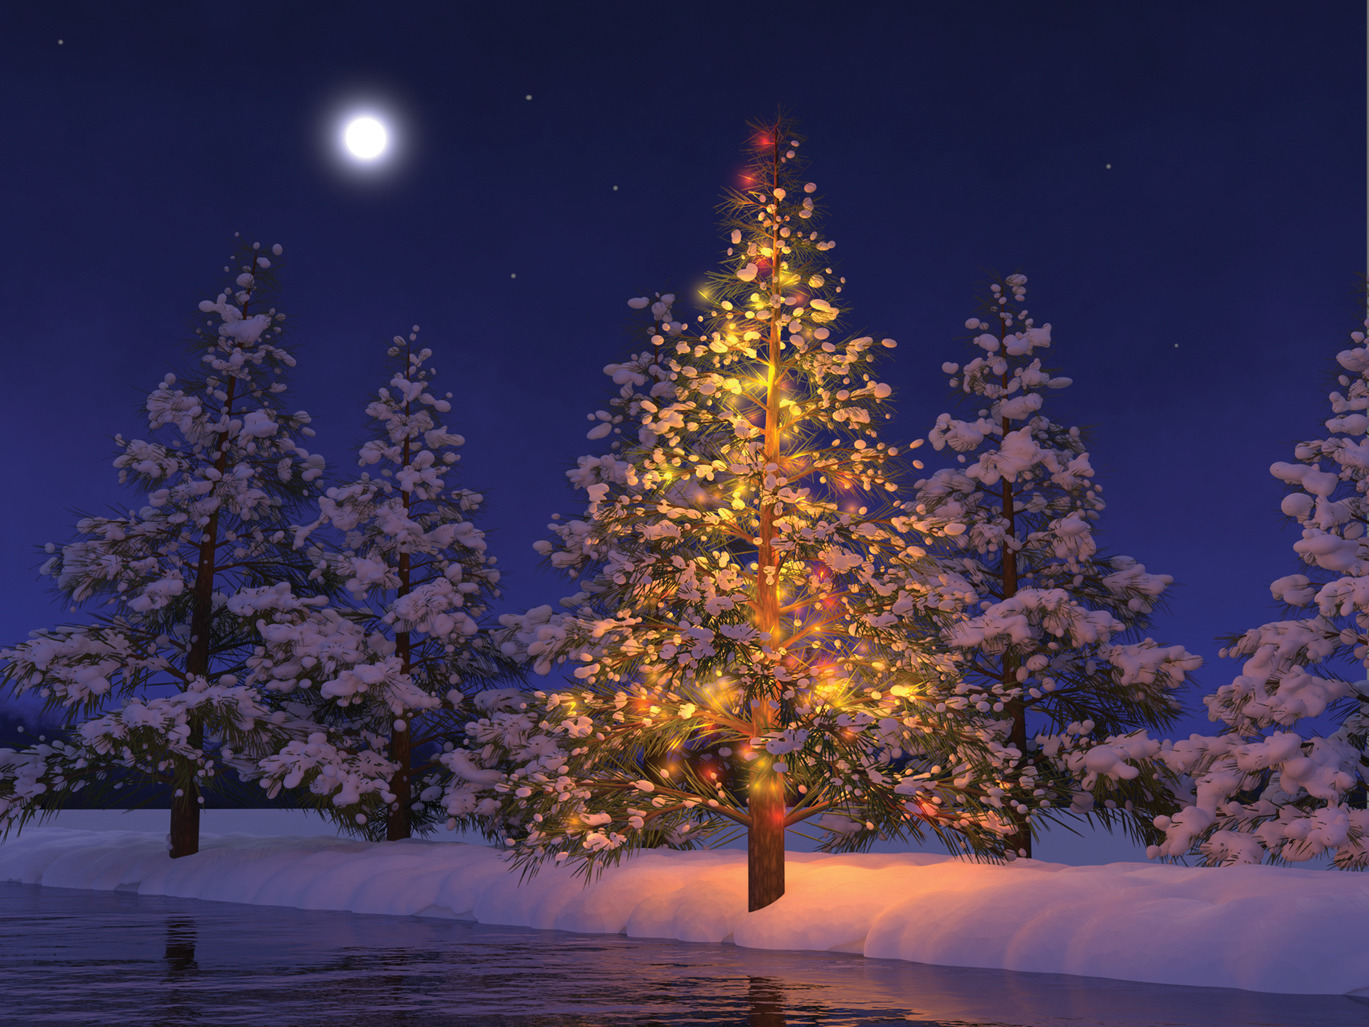
\includegraphics[width=\linewidth]{chap01/nightsnow.jpg}
    \caption{Guillaume Poncin和Pramod Sharma用许多方法扩展了pbrt,
        实现了一系列复杂渲染算法,
        制作出这张斯坦福大学CS348b渲染竞赛获奖图像。
        树木由L系统程序化建模,
        辉光图像处理滤波器增加了树上灯光的真实感,
        雪由metaball程序化建模,
        次表面散射算法考虑了光在离开雪前在雪下传播了一段距离的影响,
        赋予了雪逼真的外观。}
    \label{fig:1.11}
\end{figure}
\begin{figure}[htbp]
    \centering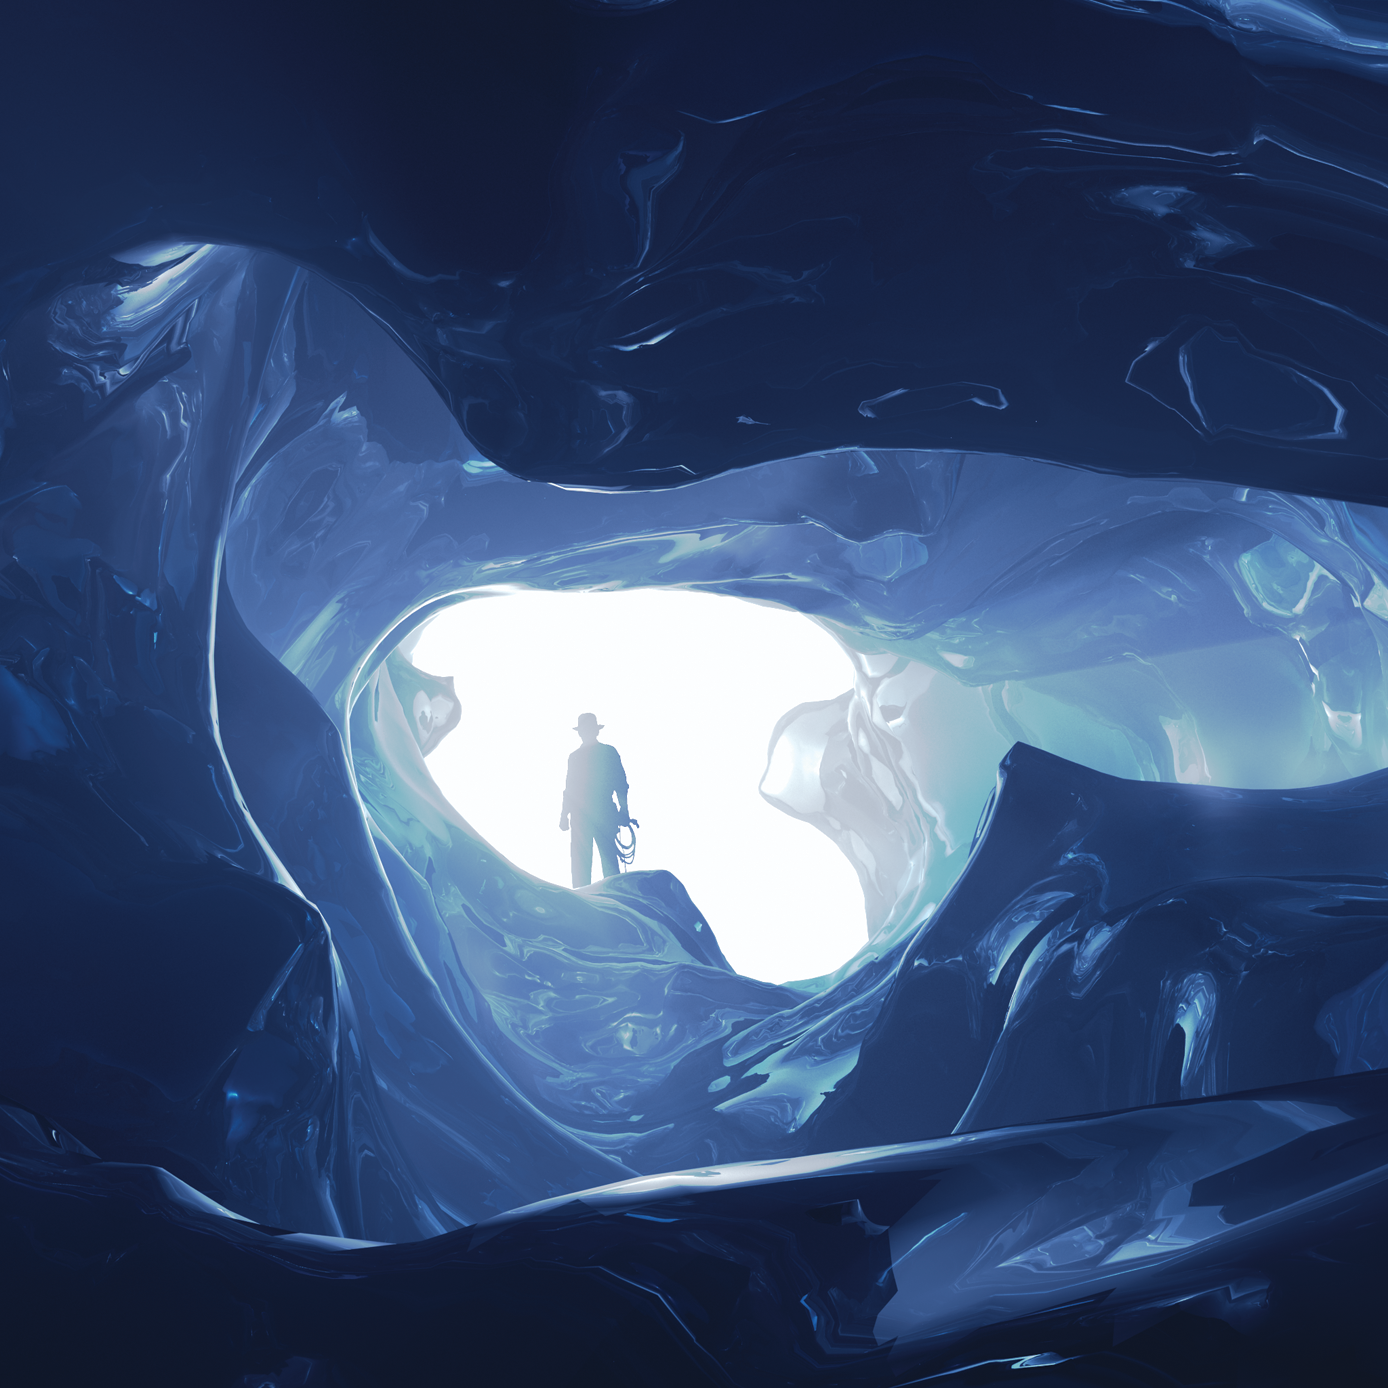
\includegraphics[width=\linewidth]{chap01/icecave.png}
    \caption{Abe Davis、David Jacobs和Jongmin Baek渲染了这张惊艳的冰窟图像,
        夺得2009斯坦福大学CS348b渲染竞赛大奖。
        他们首先实现了对冰川作用,即雪多年落下、融化、再冻结形成分层冰层这一物理过程的仿真。
        然后他们模拟了融水径流对冰的侵蚀,生成了冰的几何模型。
        体积内的光散射由体积光子映射模拟;
        冰的蓝色完全取决于在冰体中对依赖于波长的光吸收的建模。}
    \label{fig:1.12}
\end{figure}
\begin{figure}[htbp]
    \centering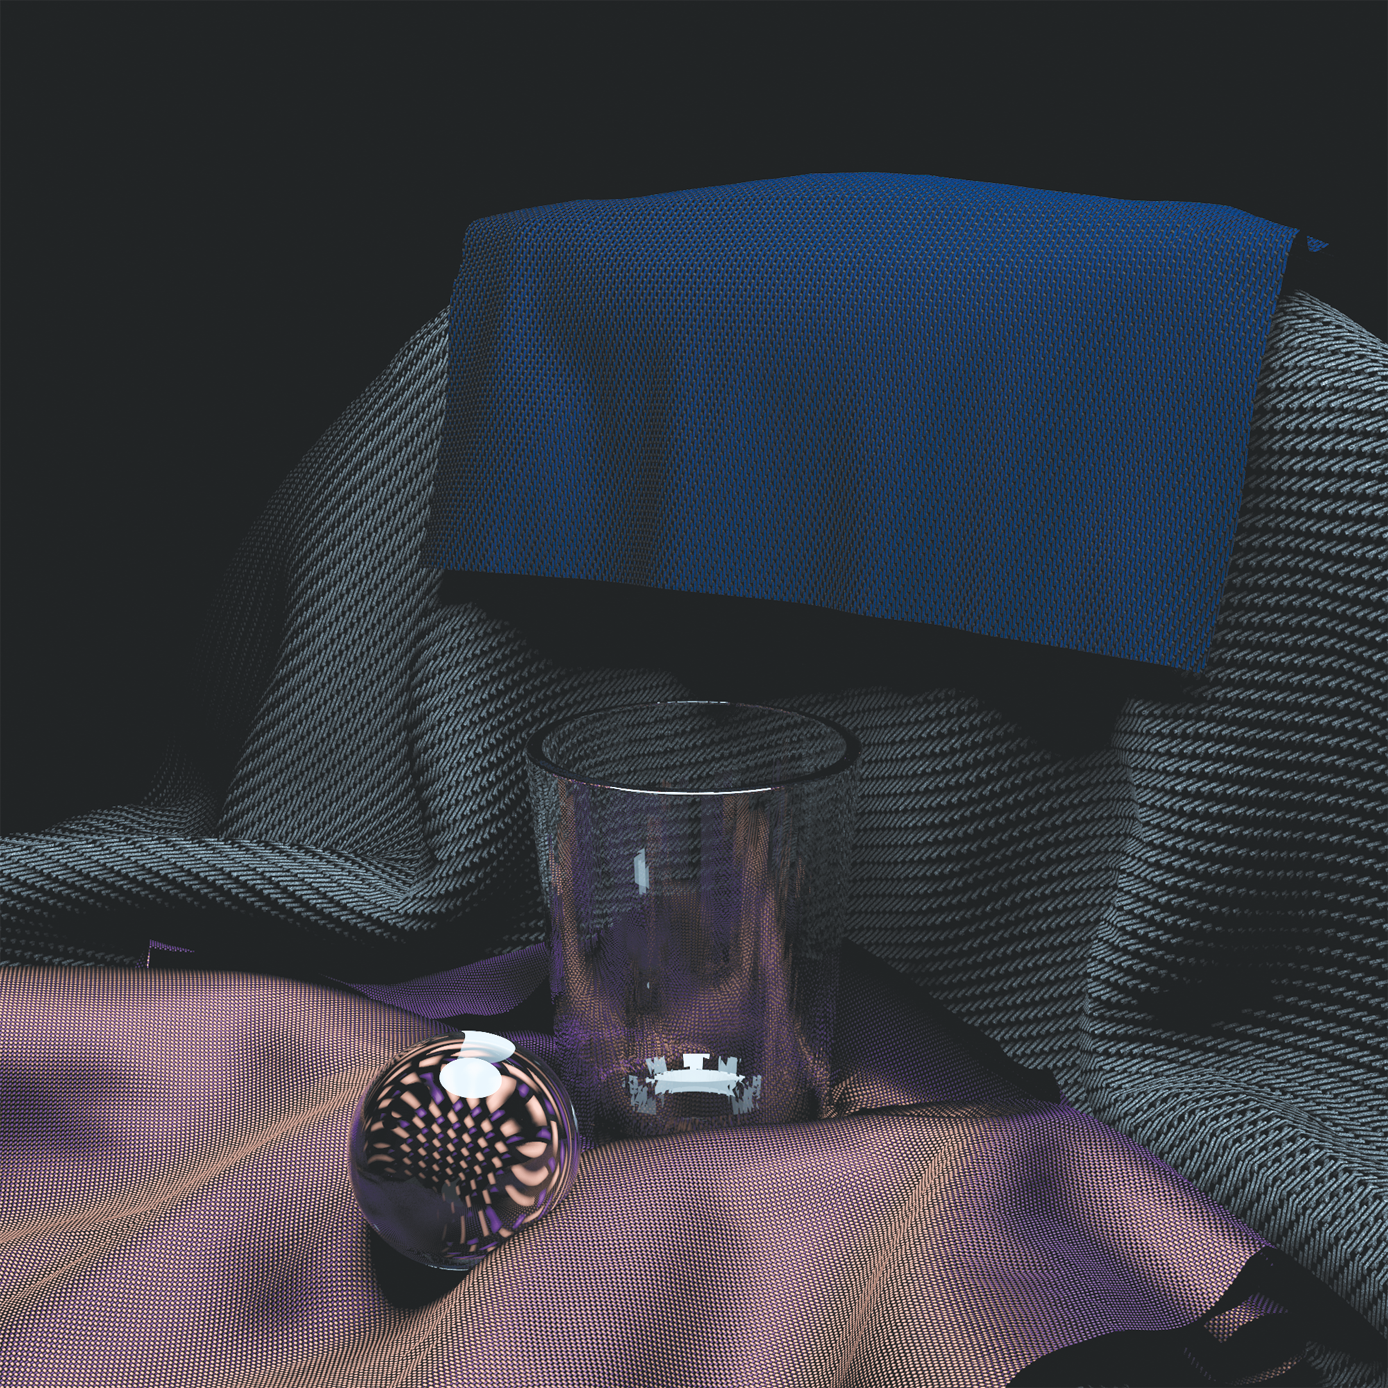
\includegraphics[width=\linewidth]{chap01/cloth.png}
    \caption{Lingfeng Yang实现了双向纹理函数来模拟布料的外观,
        添加了解析的自阴影模型,
        渲染了这张2009斯坦福大学CS348b渲染竞赛一等奖图像。}
    \label{fig:1.13}
\end{figure}

\subsection{执行阶段}\label{sub:执行阶段}

pbrt在概念上可分为两个执行阶段。
首先,解析用户提供的场景描述文件。
场景描述是一个文本文件,
指定了构成场景的几何形状及其材质属性、
对其照明的光源、虚拟相机在场景中的摆放位置、
整个系统所用的各个算法的参数等。
输入文件的每个语句都直接映射到
附录第\refchap{场景描述接口}
\sidenote{译者注:原书此处似乎链接错误,已纠正。}
中的一个例程;
这些例程包含了描述场景的程序接口。
场景文件格式的文档详见pbrt网站\href{https://pbrt.org/}{\ttfamily pbrt.org}。

解析阶段的最终结果是类\refvar{Scene}{}和\refvar{Integrator}{}的实例。
\refvar{Scene}{}包含了场景内容(几何物体、光源等)的表示,
\refvar{Integrator}{}则实现渲染它的算法。称之为\keyindex{积分器}{integrator}{}就是因为
它的主要任务是计算\refeq{1.1}的积分。

一旦指定好场景,第二执行阶段就开始了,执行主渲染循环。
pbrt通常把绝大部分运行时间都花在这个阶段,
本书大部分都在讲解执行这一阶段的代码。
渲染循环由\refvar{Integrator::Render}{()}的
实现来执行,它是\refsub{主渲染循环}的重点。

本章将介绍\refvar{Integrator}{}的一个特定子类,
称为\refvar{SamplerIntegrator}{},
其{\ttfamily Render()}方法为大量建模成像过程的光线
确定到达虚拟胶片平面的光量。
在计算完所有这些胶片样本的贡献后,把最终图像写入文件。
内存里的场景描述数据被释放,
系统从场景描述文件恢复处理语句直到没有剩余,
如果需要,用户可以指定下一个要渲染的场景。

\begin{figure}[htbp]
    \centering\includegraphics[width=\linewidth]{chap01/furrydog.png}
    \caption{Jared Jacobs和Michael Turitzin为pbrt增加了
        Kajiya和Kay基于纹素的毛发渲染算法\parencite*{10.1145/74333.74361}并渲染了该图像,
        狗毛和粗毛地毯都是用纹素毛发算法渲染的。}
    \label{fig:1.14}
\end{figure}

\reffig{1.15}和\reffig{1.16}由\emph{LuxCoreRender}渲染,
它是最初基于本书第一版pbrt源码的GPL许可的基于物理的渲染系统
(关于\emph{LuxCoreRender}的更多信息详见\url{https://luxcorerender.org}
\sidenote{译者注:原文的LuxRender现已更名为LuxCoreRender且
    迁移到了新网址,此处已更正。})。

\begin{figure}[htbp]
    \centering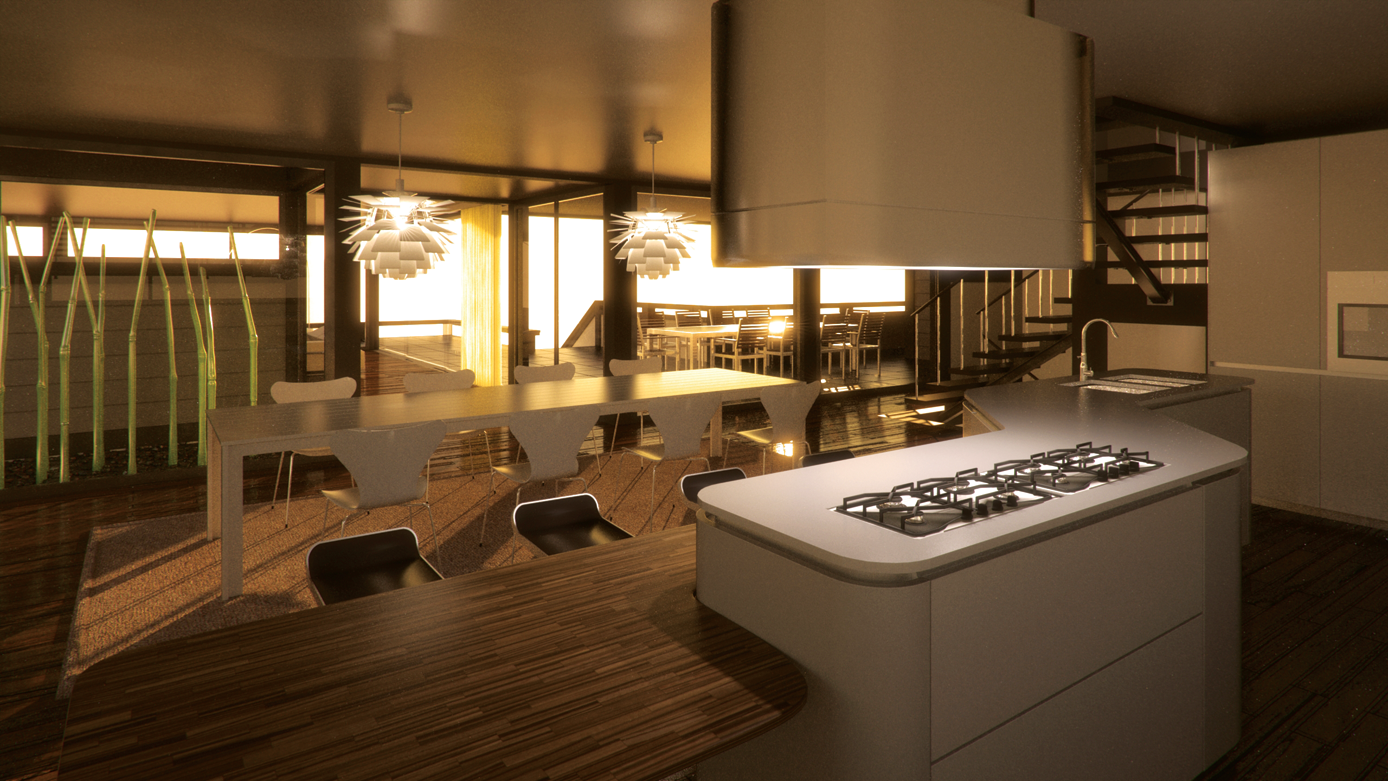
\includegraphics[width=\linewidth]{chap01/measure-one180-cut1260.png}
    \caption{Florent Boyer渲染了这个当代室内场景。
        该图像由\emph{LuxRender}渲染,它是最初
        基于pbrt源码的GPL许可的基于物理的渲染系统。
        建模和纹理由Blender完成。}
    \label{fig:1.15}
\end{figure}

\begin{figure}[htbp]
    \centering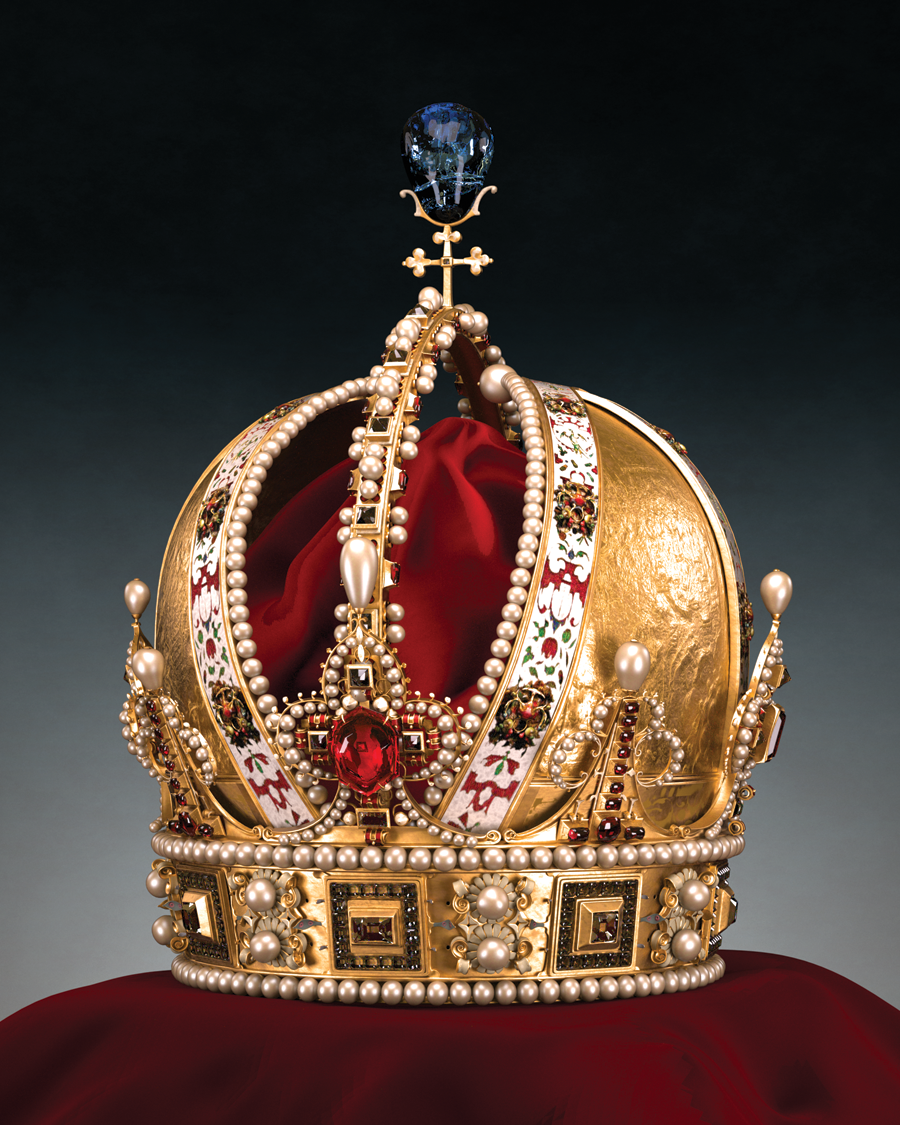
\includegraphics[width=\linewidth]{chap01/crown.png}
    \caption{Martin Lubich构建了这个奥地利皇冠的场景
        并用pbrt代码库的开源分支\emph{LuxRender}渲染了它。
        该场景由Blender建模,包含约一百八十万个顶点。
        它由具备基于真实世界光源测量数据的发射光谱的六个面光源照明,
        在四核CPU上对每个像素做1280次采样经73小时的计算完成渲染。
        包括可下载的Blender场景文件在内的更多信息
        详见Martin的网站\url{www.loramel.net}。}
    \label{fig:1.16}
\end{figure}

\subsection{场景表示}\label{sub:场景表示}
pbrt的函数\refvar{main}{()}可在
文件\href{https://github.com/mmp/pbrt-v3/tree/master/src/main/pbrt.cpp}{\ttfamily main/pbrt.cpp}内找到。
该函数很简单;
它首先循环读取{\ttfamily argv}中的命令行参数,
初始化结构体{\ttfamily Options}中的值并
保存参数中的文件名。
运行pbrt时带命令行参数{\ttfamily {-}{-}help}会
打印所有可指定的命令行选项。
解析命令行参数的代码片\refcode{Process command-line arguments}{}很简单,
故本书不再介绍\sidenote{译者注:我还是把它搬上来了。}。

选项结构体随后传入函数\refvar{pbrtInit}{()},做全系统初始化。
函数\refvar{main}{()}再解析给定场景描述,
创建\refvar{Scene}{}和\refvar{Integrator}{}。
\refvar{pbrtCleanup}{()}在系统完成所有渲染后退出前做最后的清理工作。

函数\refvar{pbrtInit}{()}和\refvar{pbrtCleanup}{()}出现在
页边空白处的迷你索引内,还注明了真正定义它们的页数。
每页的迷你索引都指向了所用的几乎所有函数、类、方法和成员变量的定义
\sidenote{译者注:在线版已经全部改用超链接了。翻译时尽力还原了在线版的跳转功能。试试看吧!}。
\begin{lstlisting}
`\initcode{Main program}{=}`
int `\initvar{main}{}`(int argc, char *argv[]) {
    Options options;
    std::vector<std::string> filenames;
    `\refcode{Process command-line arguments}{}`
    `\refvar{pbrtInit}{}`(options);
    `\refcode{Process scene description}{}`
    `\refvar{pbrtCleanup}{}`();
    return 0;
}
\end{lstlisting}
其中
\begin{lstlisting}
`\initcode{Process command-line arguments}{=}`
for (int i = 1; i < argc; ++i) {
    if (!strcmp(argv[i], "--ncores") || !strcmp(argv[i], "--nthreads"))
        options.nThreads = atoi(argv[++i]);
    else if (!strcmp(argv[i], "--outfile")) options.imageFile = argv[++i];
    else if (!strcmp(argv[i], "--quick")) options.quickRender = true;
    else if (!strcmp(argv[i], "--quiet")) options.quiet = true;
    else if (!strcmp(argv[i], "--verbose")) options.verbose = true;
    else if (!strcmp(argv[i], "--help") || !strcmp(argv[i], "-h")) {
        printf("usage: pbrt [--nthreads n] [--outfile filename] [--quick] [--quiet] "
               "[--verbose] [--help] <filename.pbrt> ...\n");
        return 0;
    }
    else filenames.push_back(argv[i]);
}
\end{lstlisting}

如果运行pbrt时没有提供输入文件名,
则它会从标准输入读取场景描述。
否则它就遍历提供的文件名,依次处理每个文件。
\begin{lstlisting}
`\initcode{Process scene description}{=}`
if (filenames.size() == 0) {
    `\refcode{Parse scene from standard input}{}`
} else {
    `\refcode{Parse scene from input files}{}`
}
\end{lstlisting}
函数{\initvar{ParseFile}{()}}或从标准输入或磁盘文件读入并解析场景描述文件;
如果无法打开文件则返回{\ttfamily false}。
本书不介绍解析场景描述文件的机制;
解析器的实现可在文件\href{https://github.com/mmp/pbrt-v3/blob/master/src/core/parser.h}{\ttfamily core/parser.h}和
\href{https://github.com/mmp/pbrt-v3/blob/master/src/core/parser.cpp}{\ttfamily core/parser.cpp}中找到
\sidenote{译者注:此处已更正文件名,因为原书给出的文件名已经失效了。}。
想要了解解析子系统但不熟悉这些工具的读者可以参阅Levine、Mason和Brown的著作\citep{10.5555/136311}。

我们遵循的UNIX习惯用法,以名为“{\ttfamily -}”的文件表示标准输入:
\begin{lstlisting}
`\initcode{Parse scene from standard input}{=}`
`\refvar{ParseFile}{}`("-");
\end{lstlisting}

如果无法打开特定的输入文件,则\refvar{Error}{()}例程会将此信息报告给用户。
\refvar{Error}{()}使用和{\ttfamily printf()}相同的格式化字符串语义。
\begin{lstlisting}
`\initcode{Parse scene from input files}{=}`
for (const std::string &f : filenames)
    if (!`\refvar{ParseFile}{}`(f))
        `\refvar{Error}{}`("Couldn't open scene file \"%s\"", f.c_str());
\end{lstlisting}

解析完场景文件后就创建表示场景中光源和几何图元的对象。
它们都存于\refvar{Scene}{}对象中,
由附录\refsub{世界端和渲染}的方法\refvar{RenderOptions::MakeScene}{()}创建。
类\refvar{Scene}{}在\href{https://github.com/mmp/pbrt-v3/tree/master/src/core/scene.h}{\ttfamily core/scene.h}中
声明并在\href{https://github.com/mmp/pbrt-v3/tree/master/src/core/scene.cpp}{\ttfamily core/scene.cpp}中定义。
\begin{lstlisting}
`\initcode{Scene Declarations}{=}`
class `\initvar{Scene}{}` {
public:
    `\refcode{Scene Public Methods}{}`
    `\refcode{Scene Public Data}{}`
private:
    `\refcode{Scene Private Data}{}`
};
\end{lstlisting}

\begin{lstlisting}
`\initcode{Scene Public Methods}{=}\initnext{ScenePublicMethods}`
`\refvar{Scene}{}`(std::shared_ptr<`\refvar{Primitive}{}`> `\refvar{aggregate}{}`,
      const std::vector<std::shared_ptr<`\refvar{Light}{}`>> &`\refvar{lights}{}`)
    : `\refvar{lights}{}`(`\refvar{lights}{}`), `\refvar{aggregate}{}`(`\refvar{aggregate}{}`) {
    `\refcode{Scene Constructor Implementation}{}`
}
\end{lstlisting}

场景中每个光源都由\refvar{Light}{}对象表示,
指定灯光的形状和发射能量的分布。
\refvar{Scene}{}用C++标准库中{\ttfamily shared\_ptr}实例
的一个{\ttfamily vector}来存储所有光源。
pbrt用共享指针\sidenote{译者注:原文shared pointers,是一种智能指针。}跟踪
其他实例对于对象的引用计数。
当最后一个持有引用的实例(例如这里的\refvar{Scene}{})被销毁时,
引用计数减到零,\refvar{Light}{}就可以安全释放了,而且是自动的。

尽管一些渲染器支持每个几何对象有单独的光源列表,
允许一个光源只照明场景中一部分物体,
但这种做法不符合pbrt采用的基于物理的渲染方法,
所以对于每个场景pbrt只支持单个全局列表。
系统的许多部分都需要获取光源,
所以\refvar{Scene}{}把它们置为公有成员变量。
\begin{lstlisting}
`\initcode{Scene Public Data}{=}`
std::vector<std::shared_ptr<`\refvar{Light}{}`>> `\initvar{lights}{}`;
\end{lstlisting}

场景中每个几何对象都由\refvar{Primitive}{}表示,结合了两个对象:
指定其几何结构的\refvar{Shape}{}和描述其外观
(例如物体的颜色、是否具有暗淡或光泽饰面)的\refvar{Material}{}。
所有几何图元都集中到\refvar{Scene}{}的
成员变量\refvar[aggregate]{Scene::aggregate}{}这一
单个\refvar{Primitive}{}聚合体中。
这个聚合体是一种特殊的图元,它自己持有许多对其他图元的引用。
因为它实现了\refvar{Primitive}{}接口,
所以从单个图元到系统其余部分似乎没什么区别。
聚合体的实现用加速的数据结构存储了所有场景图元,
减少对远离给定光线的图元做不必要的光线交点测试量。
\begin{lstlisting}
`\initcode{Scene Private Data}{=}\initnext{ScenePrivateData}`
std::shared_ptr<`\refvar{Primitive}{}`> `\initvar{aggregate}{}`;
\end{lstlisting}
构造函数把场景几何的边界框缓存到成员变量{\ttfamily worldBound}中。
\begin{lstlisting}
`\initcode{Scene Constructor Implementation}{=}\initnext{SceneConstructorImplementation}`
`\refvar{worldBound}{}` = aggregate->`\refvar{WorldBound}{}`();
\end{lstlisting}
\begin{lstlisting}
`\refcode{Scene Private Data}{+=}\lastcode{ScenePrivateData}`
`\refvar{Bounds3f}{}` `\initvar{worldBound}{}`;
\end{lstlisting}
可通过方法{\ttfamily WorldBound()}获取该边界。
\begin{lstlisting}
`\refcode{Scene Public Methods}{+=}\lastcode{ScenePublicMethods}`
const `\refvar{Bounds3f}{}` &WorldBound() const { return `\refvar{worldBound}{}`; }
\end{lstlisting}

一些光源实现发现在定义场景后开始渲染前做一些额外的初始化很有用。
\refvar{Scene}{}的构造函数调用其方法\refvar{Preprocess}{()}来允许它们这么做。
\begin{lstlisting}
`\refcode{Scene Constructor Implementation}{+=}\lastcode{SceneConstructorImplementation}`
for (const auto &light : `\refvar{lights}{}`)
    light->`\refvar{Preprocess}{}`(*this);
\end{lstlisting}

\refvar{Scene}{}类提供两个与光线-图元交点相关的方法。
它的\refvar[Scene::Intersect]{Intersect}{()}方法跟随给定光线到场景中并
返回表示光线是否与某一图元相交的布尔值。
如果是,它便把沿光线最近交点的信息填入提供的结构体\refvar{SurfaceInteraction}{}。
结构体\refvar{SurfaceInteraction}{}将在\refsec{图元接口与几何图元}定义。
\begin{lstlisting}
`\initcode{Scene Method Definitions}{=}\initnext{SceneMethodDefinitions}`
bool `\refvar{Scene}{}`::`\refvar[Intersect]{\initvar[Scene::Intersect]{Intersect}{}}{}`(const `\refvar{Ray}{}` &ray, `\refvar{SurfaceInteraction}{}` *isect) const {
    return `\refvar{aggregate}{}`->`\refvar{Intersect}{}`(ray, isect);
}
\end{lstlisting}
一个紧密相关的方法是\refvar{Scene::IntersectP}{()},
它沿光线检查交点的存在性但不返回任何关于这些交点的信息。
因为这个例程不需要搜索最近的交点或计算任何关于交点的额外信息,
所以它一般比\refvar{Scene::Intersect}{()}更高效。
这个例程用于阴影射线。
\begin{lstlisting}
`\refcode{Scene Method Definitions}{+=}\lastnext{SceneMethodDefinitions}`
bool `\refvar{Scene}{}`::`\refvar[IntersectP]{\initvar[Scene::IntersectP]{IntersectP}{}}{}`(const `\refvar{Ray}{}` &ray) const {
    return `\refvar{aggregate}{}`->`\refvar{IntersectP}{}`(ray);
}
\end{lstlisting}

\subsection{积分器接口与采样积分器}\label{sub:积分器接口与采样积分器}
渲染一幅场景图像由实现了\refvar{Integrator}{}接口的类的实例负责。
抽象基类\refvar{Integrator}{}定义了任何积分器必须提供的方法\refvar[Integrator::Render]{Render}{()}。
本节我们将定义一个\refvar{Integrator}{}的实现,即\refvar{SamplerIntegrator}{}。
在\href{https://github.com/mmp/pbrt-v3/tree/master/src/core/integrator.h}{\ttfamily core/integrator.h}中
定义了基本积分器接口,
积分器使用的一些实用函数在\href{https://github.com/mmp/pbrt-v3/blob/master/src/core/integrator.cpp}{\ttfamily core/integrator.cpp}中。
不同积分器的实现在目录\href{https://github.com/mmp/pbrt-v3/tree/master/src/integrators}{\ttfamily integrators}中。
\begin{lstlisting}
`\initcode{Integrator Declarations}{=}`
class `\initvar{Integrator}{}` {
public:
    `\refcode{Integrator Interface}{}`
};
\end{lstlisting}

\refvar{Integrator}{}必须提供方法\refvar[Integrator::Render]{Render}{()};
它利用传入的\refvar{Scene}{}引用计算一幅场景图像,
或者更一般地说,一组场景光照的度量。
其接口专门保持高度一般性以便允许各种实现——
例如可以把\refvar{Integrator}{}实现成只度量
分布于场景中的一组稀疏位置,而不是生成常规的2D图像。
\begin{lstlisting}
`\initcode{Integrator Interface}{=}`
virtual void `\initvar[Integrator::Render]{Render}{}`(const `\refvar{Scene}{}` &scene) = 0;
\end{lstlisting}

本章中,我们的重点是\refvar{Integrator}{}的一个子类\refvar{SamplerIntegrator}{},
以及实现了\refvar{SamplerIntegrator}{}接口的\refvar{WhittedIntegrator}{}
(\refvar{SamplerIntegrator}{}
的其他实现会在第\refchap{光传输I:表面反射}和\refchap{光传输II:体积渲染}介绍;
第\refchap{光传输III:双向方法}的积分器直接从\refvar{Integrator}{}继承)。
\refvar{SamplerIntegrator}{}的名字源自其渲染过程是
由来自\refvar{Sampler}{}的\keyindex{样本}{sample}{}流驱动的;
每个这样的样本都标识了图像上的一点,
让积分器计算到达该点以构成图像的光量。
\begin{lstlisting}
`\initcode{SamplerIntegrator Declarations}{=}`
class `\initvar{SamplerIntegrator}{}` : public `\refvar{Integrator}{}` {
public:
    `\refcode{SamplerIntegrator Public Methods}{}`
protected:
    `\refcode{SamplerIntegrator Protected Data}{}`
private:
    `\refcode{SamplerIntegrator Private Data}{}`
};
\end{lstlisting}

\refvar{SamplerIntegrator}{}保存了指向\refvar{Sampler}{}的指针。
采样器看似存在感低,但它的实现会极大影响系统生成图像的质量。
首先,采样器负责选取光线要追踪的图像平面上的点。
其次,它负责为积分器提供用于计算光传输积分即\refeq{1.1}的值所需的采样位置。
例如,一些积分器需要对光源选取随机位置来计算来自面光源的照明。
生成分布良好的样本在渲染过程中很重要,会极大影响整体效率;
这是第\refchap{采样与重构}的主要内容。
\begin{lstlisting}
`\initcode{SamplerIntegrator Private Data}{=}`
std::shared_ptr<`\refvar{Sampler}{}`> `\initvar{sampler}{}`;
\end{lstlisting}

对象\refvar{Camera}{}控制视角和透镜参数,例如位置、朝向、焦点和视野。
\refvar{Camera}{}内的成员变量\refvar{Film}{}执行图像存储。
\refvar{Camera}{}类将在第\refchap{相机模型}介绍,
\refvar{Film}{}将在\refsec{胶片与成像管道}介绍。
\refvar{Film}{}负责把最终图像写入文件并可能在完成计算后在屏幕上将其显示出来。
\begin{lstlisting}
`\initcode{SamplerIntegrator Protected Data}{=}`
std::shared_ptr<const `\refvar{Camera}{}`> `\initvar{camera}{}`;
\end{lstlisting}

\refvar{SamplerIntegrator}{}构造函数在成员变量中保存了指向这些对象的指针。
它在\refvar{pbrtWorldEnd}{()}调用的
方法\refvar{RenderOptions::MakeIntegrator}{()}里创建,
而\refvar{pbrtWorldEnd}{()}在输入文件解析器
完成对输入文件的场景描述解析并准备渲染场景时被调用。
\begin{lstlisting}
`\initcode{SamplerIntegrator Public Methods}{=}\initnext{SamplerIntegratorPublicMethods}`
`\refvar{SamplerIntegrator}{}`(std::shared_ptr<const `\refvar{Camera}{}`> `\refvar{camera}{}`,
    std::shared_ptr<`\refvar{Sampler}{}`> `\refvar{sampler}{}`)
    : `\refvar{camera}{}`(`\refvar{camera}{}`), `\refvar{sampler}{}`(`\refvar{sampler}{}`) { }
\end{lstlisting}

\refvar{SamplerIntegrator}{}可选实现方法\refvar[SamplerIntegrator::Preprocess]{Preprocess}{()}。
它在\refvar{Scene}{}完全初始化后被调用,
并给积分器机会完成依赖于场景的计算,
例如分配依赖于场景光源数目的额外数据结构,
或者预计算场景中辐射分布的大致表示。
在这里不需要做任何事的实现可以将这个方法留为未实现状态。
\begin{lstlisting}
`\refcode{SamplerIntegrator Public Methods}{=}\lastnext{SamplerIntegratorPublicMethods}`
virtual void `\initvar[SamplerIntegrator::Preprocess]{Preprocess}{}`(const `\refvar{Scene}{}` &scene, `\refvar{Sampler}{}` &sampler) { }
\end{lstlisting}

\subsection{主渲染循环}\label{sub:主渲染循环}
完成\refvar{Scene}{}和\refvar{Integrator}{}的分配与初始化后,
调用方法\refvar{Integrator::Render}{()},
开始pbrt的第二执行阶段:主渲染循环。
在\refvar{SamplerIntegrator}{}对该方法的实现中,
对于图像平面上的每一个位置,
该方法用\refvar{Camera}{}和\refvar{Sampler}{}生成到场景中的光线,
再用方法{\ttfamily Li()}确定沿该光线到达图像平面的光量。
该值传入\refvar{Film}{},记录下光的贡献度。
\reffig{1.17}总结了该方法用到的主要类和它们之间的数据流。
\begin{figure}[htbp]
    \centering%LaTeX with PSTricks extensions
%%Creator: Inkscape 1.0.1 (3bc2e813f5, 2020-09-07)
%%Please note this file requires PSTricks extensions
\psset{xunit=.5pt,yunit=.5pt,runit=.5pt}
\begin{pspicture}(893.08001709,262.91000366)
{
\newrgbcolor{curcolor}{0.80000001 0.80000001 0.80000001}
\pscustom[linestyle=none,fillstyle=solid,fillcolor=curcolor]
{
\newpath
\moveto(11.6500001,262.91000366)
\lineto(109.81000376,262.91000366)
\curveto(112.58000376,262.91000366)(114.81000376,260.68000366)(114.81000376,257.91000366)
\lineto(114.81000376,236.75000381)
\curveto(114.81000376,233.98000381)(112.58000376,231.75000381)(109.81000376,231.75000381)
\lineto(11.6500001,231.75000381)
\curveto(8.8800001,231.75000381)(6.6500001,233.98000381)(6.6500001,236.75000381)
\lineto(6.6500001,257.91000366)
\curveto(6.6500001,260.68000366)(8.8800001,262.91000366)(11.6500001,262.91000366)
\closepath
}
}
{
\newrgbcolor{curcolor}{0.80000001 0.80000001 0.80000001}
\pscustom[linestyle=none,fillstyle=solid,fillcolor=curcolor]
{
\newpath
\moveto(253.1499939,262.91000366)
\lineto(338.71999359,262.91000366)
\curveto(341.48999359,262.91000366)(343.71999359,260.68000366)(343.71999359,257.91000366)
\lineto(343.71999359,236.75000381)
\curveto(343.71999359,233.98000381)(341.48999359,231.75000381)(338.71999359,231.75000381)
\lineto(253.1499939,231.75000381)
\curveto(250.3799939,231.75000381)(248.1499939,233.98000381)(248.1499939,236.75000381)
\lineto(248.1499939,257.91000366)
\curveto(248.1499939,260.68000366)(250.3799939,262.91000366)(253.1499939,262.91000366)
\closepath
}
}
{
\newrgbcolor{curcolor}{0.80000001 0.80000001 0.80000001}
\pscustom[linestyle=none,fillstyle=solid,fillcolor=curcolor]
{
\newpath
\moveto(45.43999863,139.91000366)
\lineto(395.49999619,139.91000366)
\curveto(398.26999619,139.91000366)(400.49999619,137.68000366)(400.49999619,134.91000366)
\lineto(400.49999619,113.75000381)
\curveto(400.49999619,110.98000381)(398.26999619,108.75000381)(395.49999619,108.75000381)
\lineto(45.43999863,108.75000381)
\curveto(42.66999863,108.75000381)(40.43999863,110.98000381)(40.43999863,113.75000381)
\lineto(40.43999863,134.91000366)
\curveto(40.43999863,137.68000366)(42.66999863,139.91000366)(45.43999863,139.91000366)
\closepath
}
}
{
\newrgbcolor{curcolor}{0.80000001 0.80000001 0.80000001}
\pscustom[linestyle=none,fillstyle=solid,fillcolor=curcolor]
{
\newpath
\moveto(189.27999878,31.16000366)
\lineto(249.93000031,31.16000366)
\curveto(252.70000031,31.16000366)(254.93000031,28.93000366)(254.93000031,26.16000366)
\lineto(254.93000031,5.00000381)
\curveto(254.93000031,2.23000381)(252.70000031,0.00000381)(249.93000031,0.00000381)
\lineto(189.27999878,0.00000381)
\curveto(186.50999878,0.00000381)(184.27999878,2.23000381)(184.27999878,5.00000381)
\lineto(184.27999878,26.16000366)
\curveto(184.27999878,28.93000366)(186.50999878,31.16000366)(189.27999878,31.16000366)
\closepath
}
}
{
\newrgbcolor{curcolor}{0.80000001 0.80000001 0.80000001}
\pscustom[linestyle=none,fillstyle=solid,fillcolor=curcolor]
{
\newpath
\moveto(588.40002441,143.66000366)
\lineto(888.08001709,143.66000366)
\curveto(890.85001709,143.66000366)(893.08001709,141.43000366)(893.08001709,138.66000366)
\lineto(893.08001709,117.50000381)
\curveto(893.08001709,114.73000381)(890.85001709,112.50000381)(888.08001709,112.50000381)
\lineto(588.40002441,112.50000381)
\curveto(585.63002441,112.50000381)(583.40002441,114.73000381)(583.40002441,117.50000381)
\lineto(583.40002441,138.66000366)
\curveto(583.40002441,141.43000366)(585.63002441,143.66000366)(588.40002441,143.66000366)
\closepath
}
}
{
\newrgbcolor{curcolor}{0 0 0}
\pscustom[linewidth=1,linecolor=curcolor]
{
\newpath
\moveto(58.49000168,231.00000381)
\lineto(139.80999756,148.27000427)
}
}
{
\newrgbcolor{curcolor}{0 0 0}
\pscustom[linestyle=none,fillstyle=solid,fillcolor=curcolor]
{
\newpath
\moveto(132.44,147.92000366)
\lineto(139.35,148.74000366)
\lineto(140.29,155.63000366)
\lineto(145.49,142.50000366)
\closepath
}
}
{
\newrgbcolor{curcolor}{0.65098041 0.65098041 0.65098041}
\pscustom[linestyle=none,fillstyle=solid,fillcolor=curcolor]
{
\newpath
\moveto(144.57,143.43000366)
\lineto(139.8,148.29000366)
\lineto(134.39,147.65000366)
\closepath
}
}
{
\newrgbcolor{curcolor}{0.40000001 0.40000001 0.40000001}
\pscustom[linestyle=none,fillstyle=solid,fillcolor=curcolor]
{
\newpath
\moveto(139.8,148.29000366)
\lineto(140.53,153.68000366)
\lineto(144.57,143.43000366)
\closepath
}
}
{
\newrgbcolor{curcolor}{0 0 0}
\pscustom[linewidth=1,linecolor=curcolor]
{
\newpath
\moveto(251.97000122,141.52000427)
\lineto(287.11999512,221.98000336)
}
}
{
\newrgbcolor{curcolor}{0 0 0}
\pscustom[linestyle=none,fillstyle=solid,fillcolor=curcolor]
{
\newpath
\moveto(290.2,215.28000366)
\lineto(286.86,221.38000366)
\lineto(280.11,219.68000366)
\lineto(290.37,229.40000366)
\closepath
}
}
{
\newrgbcolor{curcolor}{0.65098041 0.65098041 0.65098041}
\pscustom[linestyle=none,fillstyle=solid,fillcolor=curcolor]
{
\newpath
\moveto(289.84,228.20000366)
\lineto(287.11,221.96000366)
\lineto(289.72,217.19000366)
\closepath
}
}
{
\newrgbcolor{curcolor}{0.40000001 0.40000001 0.40000001}
\pscustom[linestyle=none,fillstyle=solid,fillcolor=curcolor]
{
\newpath
\moveto(289.84,228.20000366)
\lineto(287.11,221.96000366)
\lineto(281.84,220.63000366)
\closepath
}
}
{
\newrgbcolor{curcolor}{0 0 0}
\pscustom[linewidth=1,linecolor=curcolor]
{
\newpath
\moveto(285.20999146,148.95000458)
\lineto(320.35998535,229.41000366)
}
}
{
\newrgbcolor{curcolor}{0 0 0}
\pscustom[linestyle=none,fillstyle=solid,fillcolor=curcolor]
{
\newpath
\moveto(292.22,151.24000366)
\lineto(285.47,149.54000366)
\lineto(282.13,155.65000366)
\lineto(281.96,141.52000366)
\closepath
}
}
{
\newrgbcolor{curcolor}{0.65098041 0.65098041 0.65098041}
\pscustom[linestyle=none,fillstyle=solid,fillcolor=curcolor]
{
\newpath
\moveto(282.49,142.72000366)
\lineto(285.22,148.96000366)
\lineto(290.49,150.30000366)
\closepath
}
}
{
\newrgbcolor{curcolor}{0.40000001 0.40000001 0.40000001}
\pscustom[linestyle=none,fillstyle=solid,fillcolor=curcolor]
{
\newpath
\moveto(282.61,153.74000366)
\lineto(282.49,142.72000366)
\lineto(285.22,148.96000366)
\closepath
}
}
{
\newrgbcolor{curcolor}{0 0 0}
\pscustom[linewidth=1,linecolor=curcolor]
{
\newpath
\moveto(220.03999329,108)
\lineto(220.03999329,40.3500061)
}
}
{
\newrgbcolor{curcolor}{0 0 0}
\pscustom[linestyle=none,fillstyle=solid,fillcolor=curcolor]
{
\newpath
\moveto(214.53,45.26000366)
\lineto(220.04,41.00000366)
\lineto(225.54,45.26000366)
\lineto(220.04,32.25000366)
\closepath
}
}
{
\newrgbcolor{curcolor}{0.65098041 0.65098041 0.65098041}
\pscustom[linestyle=none,fillstyle=solid,fillcolor=curcolor]
{
\newpath
\moveto(220.04,33.56000366)
\lineto(220.04,40.37000366)
\lineto(215.73,43.70000366)
\closepath
}
}
{
\newrgbcolor{curcolor}{0.40000001 0.40000001 0.40000001}
\pscustom[linestyle=none,fillstyle=solid,fillcolor=curcolor]
{
\newpath
\moveto(224.33,43.70000366)
\lineto(220.04,33.56000366)
\lineto(220.04,40.37000366)
\closepath
}
}
{
\newrgbcolor{curcolor}{0 0 0}
\pscustom[linewidth=1,linecolor=curcolor]
{
\newpath
\moveto(404.23999023,132)
\lineto(570.14001465,132)
}
}
{
\newrgbcolor{curcolor}{0 0 0}
\pscustom[linestyle=none,fillstyle=solid,fillcolor=curcolor]
{
\newpath
\moveto(565.23,126.49000366)
\lineto(569.49,132.00000366)
\lineto(565.23,137.50000366)
\lineto(578.24,132.00000366)
\closepath
}
}
{
\newrgbcolor{curcolor}{0.65098041 0.65098041 0.65098041}
\pscustom[linestyle=none,fillstyle=solid,fillcolor=curcolor]
{
\newpath
\moveto(576.93,132.00000366)
\lineto(570.12,132.00000366)
\lineto(566.79,127.69000366)
\closepath
}
}
{
\newrgbcolor{curcolor}{0.40000001 0.40000001 0.40000001}
\pscustom[linestyle=none,fillstyle=solid,fillcolor=curcolor]
{
\newpath
\moveto(566.79,136.29000366)
\lineto(576.93,132.00000366)
\lineto(570.12,132.00000366)
\closepath
}
}
{
\newrgbcolor{curcolor}{0 0 0}
\pscustom[linewidth=1,linecolor=curcolor]
{
\newpath
\moveto(413.83999634,117.75)
\lineto(579.73999023,117.75)
}
}
{
\newrgbcolor{curcolor}{0 0 0}
\pscustom[linestyle=none,fillstyle=solid,fillcolor=curcolor]
{
\newpath
\moveto(418.75,112.24000366)
\lineto(414.5,117.75000366)
\lineto(418.75,123.25000366)
\lineto(405.74,117.75000366)
\closepath
}
}
{
\newrgbcolor{curcolor}{0.65098041 0.65098041 0.65098041}
\pscustom[linestyle=none,fillstyle=solid,fillcolor=curcolor]
{
\newpath
\moveto(413.87,117.75000366)
\lineto(417.2,113.44000366)
\lineto(407.05,117.75000366)
\closepath
}
}
{
\newrgbcolor{curcolor}{0.40000001 0.40000001 0.40000001}
\pscustom[linestyle=none,fillstyle=solid,fillcolor=curcolor]
{
\newpath
\moveto(413.87,117.75000366)
\lineto(417.2,122.04000366)
\lineto(407.05,117.75000366)
\closepath
}
}
{
\newrgbcolor{curcolor}{0 0 0}
\pscustom[linestyle=none,fillstyle=solid,fillcolor=curcolor]
{
\newpath
\moveto(18.83423174,243.34563524)
\curveto(18.64673203,243.12341337)(18.4939545,242.98105249)(18.37589913,242.91855258)
\curveto(18.26478819,242.85605268)(18.12589952,242.82480273)(17.95923312,242.82480273)
\curveto(17.63284475,242.82480273)(17.36895627,242.93244145)(17.1675677,243.14771889)
\curveto(16.97312357,243.36994076)(16.8759015,243.73452352)(16.8759015,244.24146716)
\lineto(16.8759015,245.67896489)
\curveto(16.8759015,246.19285297)(16.97312357,246.55743573)(17.1675677,246.77271316)
\curveto(17.36895627,246.99493503)(17.63284475,247.10604597)(17.95923312,247.10604597)
\curveto(18.20923272,247.10604597)(18.41756573,247.04007385)(18.58423213,246.90812962)
\curveto(18.75784297,246.77618538)(18.8897872,246.55396351)(18.98006484,246.241464)
\curveto(19.07034248,245.93590893)(19.16409233,245.72757592)(19.2613144,245.61646499)
\curveto(19.46270297,245.40118755)(19.82034129,245.1824379)(20.33422937,244.96021603)
\curveto(20.84811745,244.73799415)(21.41061656,244.62688322)(22.0217267,244.62688322)
\curveto(22.97311409,244.62688322)(23.75436285,244.84910509)(24.365473,245.29354883)
\curveto(24.75436128,245.56438174)(24.94880541,245.89771454)(24.94880541,246.29354725)
\curveto(24.94880541,246.55743573)(24.85505556,246.80396311)(24.66755586,247.03312942)
\curveto(24.48005615,247.26924016)(24.17450108,247.46368429)(23.75089064,247.61646183)
\curveto(23.4731133,247.72062833)(22.8515865,247.86298922)(21.88631025,248.04354449)
\curveto(20.71964543,248.25882193)(19.83770237,248.51923818)(19.2404811,248.82479325)
\curveto(18.64325982,249.13034833)(18.17103834,249.5609032)(17.82381667,250.11645788)
\curveto(17.47659499,250.67201256)(17.30298416,251.27270606)(17.30298416,251.91853837)
\curveto(17.30298416,252.93937009)(17.73006681,253.83172979)(18.58423213,254.59561747)
\curveto(19.43839745,255.36644959)(20.54950681,255.75186565)(21.9175602,255.75186565)
\curveto(22.46617044,255.75186565)(22.97311409,255.68936575)(23.43839113,255.56436594)
\curveto(23.91061261,255.44631057)(24.33769527,255.26228309)(24.71963911,255.01228348)
\curveto(24.99741645,255.28311639)(25.27519379,255.41853284)(25.55297112,255.41853284)
\curveto(25.86547063,255.41853284)(26.11894245,255.3074219)(26.31338659,255.08520003)
\curveto(26.51477516,254.8699226)(26.61546945,254.50881205)(26.61546945,254.00186841)
\lineto(26.61546945,252.39770428)
\curveto(26.61546945,251.8838162)(26.51477516,251.51576123)(26.31338659,251.29353936)
\curveto(26.11894245,251.07826192)(25.86547063,250.9706232)(25.55297112,250.9706232)
\curveto(25.28908265,250.9706232)(25.05991635,251.05048418)(24.86547221,251.21020615)
\curveto(24.71269467,251.32826152)(24.59811152,251.56437226)(24.52172275,251.91853837)
\curveto(24.44533399,252.27270448)(24.34811192,252.5261763)(24.23005655,252.67895383)
\curveto(24.02866798,252.94284231)(23.72658512,253.16506418)(23.32380798,253.34561945)
\curveto(22.92103084,253.52617472)(22.45575379,253.61645235)(21.92797685,253.61645235)
\curveto(21.15714473,253.61645235)(20.54603459,253.43589708)(20.09464641,253.07478654)
\curveto(19.65020267,252.72062043)(19.4279808,252.34909324)(19.4279808,251.96020497)
\curveto(19.4279808,251.6963165)(19.51825843,251.43937246)(19.6988137,251.18937285)
\curveto(19.88631341,250.94631768)(20.15714631,250.75534576)(20.51131242,250.61645709)
\curveto(20.74742316,250.51923502)(21.41061656,250.36298527)(22.50089261,250.14770783)
\curveto(23.5981131,249.93243039)(24.43838955,249.69631966)(25.02172196,249.43937562)
\curveto(25.61199881,249.18243158)(26.10158137,248.77965444)(26.49046964,248.23104419)
\curveto(26.87935792,247.68243395)(27.07380206,247.0296572)(27.07380206,246.27271395)
\curveto(27.07380206,245.21716006)(26.70227486,244.3734114)(25.95922048,243.74146795)
\curveto(24.97311093,242.90813593)(23.71616847,242.49146993)(22.18839311,242.49146993)
\curveto(21.59811626,242.49146993)(21.02172828,242.56438648)(20.45922917,242.71021958)
\curveto(19.90367449,242.84910825)(19.36200868,243.06091347)(18.83423174,243.34563524)
\closepath
}
}
{
\newrgbcolor{curcolor}{0 0 0}
\pscustom[linestyle=none,fillstyle=solid,fillcolor=curcolor]
{
\newpath
\moveto(36.67795343,242.80396943)
\lineto(36.67795343,243.30396864)
\curveto(36.14323205,243.01924687)(35.55295521,242.80744165)(34.90712289,242.66855298)
\curveto(34.26129058,242.52271988)(33.67448595,242.44980332)(33.14670901,242.44980332)
\curveto(32.00087748,242.44980332)(31.0703234,242.75188618)(30.35504675,243.35605189)
\curveto(29.6397701,243.96716204)(29.28213178,244.64077209)(29.28213178,245.37688203)
\curveto(29.28213178,246.27271395)(29.73699217,247.10257375)(30.64671296,247.86646144)
\curveto(31.56337817,248.63729355)(32.82726507,249.02270961)(34.43837363,249.02270961)
\curveto(35.08420595,249.02270961)(35.83073254,248.95326527)(36.67795343,248.8143766)
\lineto(36.67795343,249.32479247)
\curveto(36.67795343,249.64423641)(36.53906476,249.90465266)(36.26128742,250.10604123)
\curveto(35.99045451,250.3074298)(35.469622,250.40812409)(34.69878989,250.40812409)
\curveto(34.06684644,250.40812409)(33.24740329,250.28312428)(32.24046044,250.03312468)
\curveto(31.86546103,249.94284704)(31.57379482,249.89770823)(31.36546182,249.89770823)
\curveto(31.08074005,249.89770823)(30.83768488,249.99840251)(30.6362963,250.19979108)
\curveto(30.44185217,250.40812409)(30.3446301,250.67201256)(30.3446301,250.9914565)
\curveto(30.3446301,251.17201177)(30.37935227,251.32826152)(30.4487966,251.46020576)
\curveto(30.51824094,251.59214999)(30.615463,251.6963165)(30.74046281,251.77270527)
\curveto(30.86546261,251.85603847)(31.12587887,251.95326054)(31.52171157,252.06437147)
\curveto(32.04948852,252.21020457)(32.58768211,252.32478773)(33.13629236,252.40812093)
\curveto(33.6849026,252.49839856)(34.18142959,252.54353738)(34.62587334,252.54353738)
\curveto(35.95226013,252.54353738)(36.98003628,252.25534339)(37.7092018,251.67895541)
\curveto(38.44531175,251.10951187)(38.81336672,250.3282631)(38.81336672,249.33520912)
\lineto(38.81336672,244.93938273)
\lineto(39.17794948,244.93938273)
\curveto(39.69183756,244.93938273)(40.05642031,244.83868844)(40.27169775,244.63729987)
\curveto(40.49391962,244.44285573)(40.60503056,244.18591169)(40.60503056,243.86646775)
\curveto(40.60503056,243.55396825)(40.49391962,243.29702421)(40.27169775,243.09563564)
\curveto(40.05642031,242.9011915)(39.69183756,242.80396943)(39.17794948,242.80396943)
\closepath
\moveto(36.67795343,246.62688006)
\curveto(35.82378811,246.79354646)(35.03559491,246.87687967)(34.31337383,246.87687967)
\curveto(33.44531965,246.87687967)(32.69879305,246.66507444)(32.07379403,246.241464)
\curveto(31.68490576,245.9706311)(31.49046162,245.69632597)(31.49046162,245.41854864)
\curveto(31.49046162,245.21716006)(31.58421147,245.05396588)(31.77171118,244.92896608)
\curveto(32.11893285,244.69979977)(32.59462655,244.58521662)(33.19879226,244.58521662)
\curveto(33.71268033,244.58521662)(34.29254053,244.6859109)(34.93837284,244.88729947)
\curveto(35.59114959,245.08868805)(36.17100978,245.36299317)(36.67795343,245.71021484)
\closepath
}
}
{
\newrgbcolor{curcolor}{0 0 0}
\pscustom[linestyle=none,fillstyle=solid,fillcolor=curcolor]
{
\newpath
\moveto(44.26127466,252.26228783)
\lineto(44.26127466,251.65812211)
\curveto(44.60849633,251.99839935)(44.92099584,252.23103787)(45.19877318,252.35603768)
\curveto(45.48349495,252.48798191)(45.80988333,252.55395403)(46.1779383,252.55395403)
\curveto(46.49043781,252.55395403)(46.7994651,252.47756526)(47.10502017,252.32478773)
\curveto(47.41057524,252.17201019)(47.70918588,251.94284389)(48.00085209,251.63728881)
\curveto(48.36890706,251.94284389)(48.74043425,252.16853797)(49.11543366,252.31437108)
\curveto(49.4973775,252.46714861)(49.88626578,252.54353738)(50.28209848,252.54353738)
\curveto(51.0737639,252.54353738)(51.716124,252.33173216)(52.20917877,251.90812172)
\curveto(52.86195552,251.35256704)(53.18834389,250.62340153)(53.18834389,249.72062517)
\lineto(53.18834389,244.93938273)
\curveto(53.63278764,244.93938273)(53.96264823,244.83868844)(54.17792566,244.63729987)
\curveto(54.3932031,244.4359113)(54.50084182,244.17896726)(54.50084182,243.86646775)
\curveto(54.50084182,243.55396825)(54.3932031,243.29702421)(54.17792566,243.09563564)
\curveto(53.96264823,242.9011915)(53.59806547,242.80396943)(53.08417739,242.80396943)
\lineto(51.0529306,242.80396943)
\lineto(51.0529306,249.54354212)
\curveto(51.0529306,249.86993049)(50.99390291,250.09562458)(50.87584755,250.22062438)
\curveto(50.75779218,250.34562419)(50.57723691,250.40812409)(50.33418173,250.40812409)
\curveto(50.098071,250.40812409)(49.87932134,250.34562419)(49.67793277,250.22062438)
\curveto(49.42098873,250.04701355)(49.10848923,249.72062517)(48.74043425,249.24145926)
\lineto(48.74043425,244.93938273)
\curveto(49.18487799,244.93938273)(49.51473858,244.83868844)(49.73001602,244.63729987)
\curveto(49.94529346,244.4359113)(50.05293218,244.17896726)(50.05293218,243.86646775)
\curveto(50.05293218,243.55396825)(49.94529346,243.29702421)(49.73001602,243.09563564)
\curveto(49.51473858,242.9011915)(49.15015583,242.80396943)(48.63626775,242.80396943)
\lineto(46.60502096,242.80396943)
\lineto(46.60502096,249.54354212)
\curveto(46.60502096,249.86298606)(46.54252106,250.08520793)(46.41752125,250.21020773)
\curveto(46.29946589,250.34215197)(46.11891061,250.40812409)(45.87585544,250.40812409)
\curveto(45.62585584,250.40812409)(45.37932845,250.3282631)(45.13627328,250.16854113)
\curveto(44.89321811,250.0157636)(44.6015519,249.70673631)(44.26127466,249.24145926)
\lineto(44.26127466,244.93938273)
\curveto(44.7057184,244.93938273)(45.03557899,244.83868844)(45.25085643,244.63729987)
\curveto(45.4730783,244.4359113)(45.58418924,244.17896726)(45.58418924,243.86646775)
\curveto(45.58418924,243.55396825)(45.4730783,243.29702421)(45.25085643,243.09563564)
\curveto(45.03557899,242.9011915)(44.67099624,242.80396943)(44.15710816,242.80396943)
\lineto(42.23002787,242.80396943)
\curveto(41.71613979,242.80396943)(41.35155703,242.9011915)(41.1362796,243.09563564)
\curveto(40.91405772,243.29702421)(40.80294679,243.55744046)(40.80294679,243.8768844)
\curveto(40.80294679,244.18938391)(40.91058551,244.44285573)(41.12586295,244.63729987)
\curveto(41.34114038,244.83868844)(41.67447319,244.93938273)(42.12586137,244.93938273)
\lineto(42.12586137,250.12687453)
\curveto(41.67447319,250.12687453)(41.34114038,250.22756882)(41.12586295,250.42895739)
\curveto(40.91058551,250.63034596)(40.80294679,250.88729)(40.80294679,251.1997895)
\curveto(40.80294679,251.51228901)(40.91405772,251.76576083)(41.1362796,251.96020497)
\curveto(41.35155703,252.16159354)(41.71613979,252.26228783)(42.23002787,252.26228783)
\closepath
}
}
{
\newrgbcolor{curcolor}{0 0 0}
\pscustom[linestyle=none,fillstyle=solid,fillcolor=curcolor]
{
\newpath
\moveto(57.70916996,243.98105091)
\lineto(57.70916996,240.48105643)
\lineto(58.99041794,240.48105643)
\curveto(59.50430602,240.48105643)(59.86888877,240.38383437)(60.08416621,240.18939023)
\curveto(60.30638808,239.98800166)(60.41749902,239.7275854)(60.41749902,239.40814146)
\curveto(60.41749902,239.09564196)(60.30638808,238.84217013)(60.08416621,238.647726)
\curveto(59.86888877,238.44633743)(59.50430602,238.34564314)(58.99041794,238.34564314)
\lineto(55.20917391,238.34564314)
\curveto(54.69528583,238.34564314)(54.32723086,238.44633743)(54.10500899,238.647726)
\curveto(53.88973155,238.84217013)(53.78209283,239.09564196)(53.78209283,239.40814146)
\curveto(53.78209283,239.7275854)(53.89320377,239.98800166)(54.11542564,240.18939023)
\curveto(54.33764751,240.38383437)(54.70223027,240.48105643)(55.20917391,240.48105643)
\lineto(55.57375667,240.48105643)
\lineto(55.57375667,250.12687453)
\lineto(55.20917391,250.12687453)
\curveto(54.69528583,250.12687453)(54.32723086,250.2240966)(54.10500899,250.41854074)
\curveto(53.88973155,250.61992931)(53.78209283,250.88034556)(53.78209283,251.1997895)
\curveto(53.78209283,251.51228901)(53.88973155,251.76576083)(54.10500899,251.96020497)
\curveto(54.32723086,252.16159354)(54.69528583,252.26228783)(55.20917391,252.26228783)
\lineto(57.70916996,252.26228783)
\lineto(57.70916996,251.53312231)
\curveto(58.20916917,251.87339955)(58.72652947,252.12687137)(59.26125084,252.29353778)
\curveto(59.79597222,252.46020418)(60.34458247,252.54353738)(60.90708158,252.54353738)
\curveto(62.36541261,252.54353738)(63.6084662,252.04701039)(64.63624235,251.0539564)
\curveto(65.66401851,250.06784685)(66.17790659,248.93590419)(66.17790659,247.65812843)
\curveto(66.17790659,246.24840844)(65.57026866,245.08521583)(64.3549928,244.16855061)
\curveto(63.34110551,243.40466293)(62.1987462,243.02271909)(60.92791488,243.02271909)
\curveto(60.37930463,243.02271909)(59.83763882,243.10258007)(59.30291744,243.26230204)
\curveto(58.76819607,243.42202401)(58.23694691,243.66160697)(57.70916996,243.98105091)
\closepath
\moveto(64.04249329,247.64771178)
\curveto(64.04249329,247.94632242)(63.92443792,248.32479404)(63.68832718,248.78312665)
\curveto(63.45221645,249.2484037)(63.08763369,249.63381975)(62.59457891,249.93937483)
\curveto(62.10846857,250.25187433)(61.53555281,250.40812409)(60.87583163,250.40812409)
\curveto(59.8133333,250.40812409)(58.96958464,250.00881916)(58.34458562,249.21020931)
\curveto(57.92097518,248.66159907)(57.70916996,248.13382212)(57.70916996,247.62687848)
\curveto(57.70916996,247.05743494)(58.01125282,246.50188026)(58.61541853,245.96021445)
\curveto(59.22652868,245.42549307)(59.97999971,245.15813238)(60.87583163,245.15813238)
\curveto(61.77860798,245.15813238)(62.53207901,245.42549307)(63.13624472,245.96021445)
\curveto(63.74041044,246.49493582)(64.04249329,247.05743494)(64.04249329,247.64771178)
\closepath
}
}
{
\newrgbcolor{curcolor}{0 0 0}
\pscustom[linestyle=none,fillstyle=solid,fillcolor=curcolor]
{
\newpath
\moveto(74.22997708,256.31436476)
\lineto(74.22997708,244.93938273)
\lineto(76.79247303,244.93938273)
\curveto(77.30636111,244.93938273)(77.67094386,244.83868844)(77.8862213,244.63729987)
\curveto(78.10844317,244.44285573)(78.21955411,244.18591169)(78.21955411,243.86646775)
\curveto(78.21955411,243.55396825)(78.10844317,243.29702421)(77.8862213,243.09563564)
\curveto(77.67094386,242.9011915)(77.30636111,242.80396943)(76.79247303,242.80396943)
\lineto(69.53206783,242.80396943)
\curveto(69.01817975,242.80396943)(68.65012478,242.9011915)(68.42790291,243.09563564)
\curveto(68.21262547,243.29702421)(68.10498675,243.55744046)(68.10498675,243.8768844)
\curveto(68.10498675,244.18938391)(68.21262547,244.44285573)(68.42790291,244.63729987)
\curveto(68.65012478,244.83868844)(69.01817975,244.93938273)(69.53206783,244.93938273)
\lineto(72.09456378,244.93938273)
\lineto(72.09456378,254.17895146)
\lineto(70.3758165,254.17895146)
\curveto(69.86887285,254.17895146)(69.5042901,254.27617353)(69.28206822,254.47061767)
\curveto(69.05984635,254.67200624)(68.94873542,254.9324225)(68.94873542,255.25186644)
\curveto(68.94873542,255.56436594)(69.05637414,255.81783776)(69.27165157,256.0122819)
\curveto(69.49387345,256.21367047)(69.86192842,256.31436476)(70.3758165,256.31436476)
\closepath
}
}
{
\newrgbcolor{curcolor}{0 0 0}
\pscustom[linestyle=none,fillstyle=solid,fillcolor=curcolor]
{
\newpath
\moveto(91.32369995,246.44979701)
\lineto(82.56329712,246.44979701)
\curveto(82.78551899,245.89424233)(83.17787949,245.44632637)(83.7403786,245.10604913)
\curveto(84.30982214,244.76577189)(85.07718204,244.59563327)(86.04245829,244.59563327)
\curveto(86.83412371,244.59563327)(87.88620538,244.76577189)(89.19870331,245.10604913)
\curveto(89.74036912,245.2449378)(90.11536853,245.31438213)(90.32370153,245.31438213)
\curveto(90.6084233,245.31438213)(90.84800626,245.21368785)(91.0424504,245.01229928)
\curveto(91.23689453,244.81091071)(91.3341166,244.55743888)(91.3341166,244.25188381)
\curveto(91.3341166,243.97410647)(91.2299501,243.73799573)(91.0216171,243.5435516)
\curveto(90.74383976,243.28660756)(90.06675749,243.04008017)(88.9903703,242.80396943)
\curveto(87.91398312,242.57480313)(86.87926253,242.46021997)(85.88620854,242.46021997)
\curveto(84.17787791,242.46021997)(82.80982451,242.9428581)(81.78204836,243.90813435)
\curveto(80.76121664,244.87341061)(80.25080078,246.06090873)(80.25080078,247.47062873)
\curveto(80.25080078,248.97062636)(80.80288324,250.18937443)(81.90704816,251.12687295)
\curveto(83.01815752,252.0713159)(84.29593327,252.54353738)(85.74037544,252.54353738)
\curveto(86.60842962,252.54353738)(87.40356726,252.39075984)(88.12578834,252.08520477)
\curveto(88.85495385,251.7796497)(89.39661966,251.44978911)(89.75078577,251.095623)
\curveto(90.25078498,250.58173492)(90.66397877,249.94631926)(90.99036715,249.18937601)
\curveto(91.21258902,248.66159907)(91.32369995,248.05048892)(91.32369995,247.35604557)
\closepath
\moveto(88.95912035,248.5852103)
\curveto(88.63273198,249.19632045)(88.20564932,249.65118084)(87.67787238,249.94979148)
\curveto(87.15009543,250.25534655)(86.5216242,250.40812409)(85.79245869,250.40812409)
\curveto(85.07023761,250.40812409)(84.44523859,250.25534655)(83.91746165,249.94979148)
\curveto(83.38968471,249.65118084)(82.95912983,249.19632045)(82.62579702,248.5852103)
\closepath
}
}
{
\newrgbcolor{curcolor}{0 0 0}
\pscustom[linestyle=none,fillstyle=solid,fillcolor=curcolor]
{
\newpath
\moveto(98.32368877,252.26228783)
\lineto(98.32368877,250.9289566)
\curveto(99.21952069,251.57478891)(99.92438069,252.00534379)(100.43826876,252.22062122)
\curveto(100.95910128,252.43589866)(101.44521162,252.54353738)(101.89659979,252.54353738)
\curveto(102.59104314,252.54353738)(103.26465319,252.28659334)(103.91742994,251.77270527)
\curveto(104.36187368,251.42548359)(104.58409555,251.07131748)(104.58409555,250.71020694)
\curveto(104.58409555,250.40465187)(104.47645683,250.14423562)(104.26117939,249.92895818)
\curveto(104.05284639,249.72062517)(103.79937457,249.61645867)(103.50076393,249.61645867)
\curveto(103.23687546,249.61645867)(102.95909812,249.74840291)(102.66743191,250.01229138)
\curveto(102.3757657,250.27617985)(102.11534945,250.40812409)(101.88618314,250.40812409)
\curveto(101.58757251,250.40812409)(101.13965655,250.22062438)(100.54243527,249.84562498)
\curveto(99.95215842,249.47062557)(99.21257626,248.90812646)(98.32368877,248.15812764)
\lineto(98.32368877,244.93938273)
\lineto(101.36535063,244.93938273)
\curveto(101.87923871,244.93938273)(102.24382147,244.83868844)(102.45909891,244.63729987)
\curveto(102.68132078,244.44285573)(102.79243171,244.18591169)(102.79243171,243.86646775)
\curveto(102.79243171,243.55396825)(102.68132078,243.29702421)(102.45909891,243.09563564)
\curveto(102.24382147,242.9011915)(101.87923871,242.80396943)(101.36535063,242.80396943)
\lineto(94.91744415,242.80396943)
\curveto(94.40355607,242.80396943)(94.0355011,242.9011915)(93.81327923,243.09563564)
\curveto(93.59800179,243.29702421)(93.49036307,243.55744046)(93.49036307,243.8768844)
\curveto(93.49036307,244.18938391)(93.59800179,244.44285573)(93.81327923,244.63729987)
\curveto(94.0355011,244.83868844)(94.40355607,244.93938273)(94.91744415,244.93938273)
\lineto(96.18827548,244.93938273)
\lineto(96.18827548,250.12687453)
\lineto(95.41744336,250.12687453)
\curveto(94.90355528,250.12687453)(94.53550031,250.2240966)(94.31327844,250.41854074)
\curveto(94.098001,250.61992931)(93.99036228,250.88034556)(93.99036228,251.1997895)
\curveto(93.99036228,251.51228901)(94.098001,251.76576083)(94.31327844,251.96020497)
\curveto(94.53550031,252.16159354)(94.90355528,252.26228783)(95.41744336,252.26228783)
\closepath
}
}
{
\newrgbcolor{curcolor}{0 0 0}
\pscustom[linestyle=none,fillstyle=solid,fillcolor=curcolor]
{
\newpath
\moveto(267.22149308,253.11645268)
\curveto(267.35343731,253.29700795)(267.4957982,253.4324244)(267.64857573,253.52270204)
\curveto(267.8082977,253.61297967)(267.97843632,253.65811849)(268.15899159,253.65811849)
\curveto(268.4714911,253.65811849)(268.72496292,253.55047977)(268.91940706,253.33520233)
\curveto(269.12079563,253.1199249)(269.22148992,252.75534214)(269.22148992,252.24145406)
\lineto(269.22148992,250.42895692)
\curveto(269.22148992,249.91506885)(269.12079563,249.54701387)(268.91940706,249.324792)
\curveto(268.72496292,249.10951456)(268.4714911,249.00187584)(268.15899159,249.00187584)
\curveto(267.87426982,249.00187584)(267.64510352,249.08173683)(267.47149268,249.2414588)
\curveto(267.29788184,249.40118077)(267.16940982,249.69979141)(267.08607662,250.13729072)
\curveto(267.03746559,250.42895692)(266.94024352,250.65465101)(266.79441042,250.81437298)
\curveto(266.50968864,251.12687249)(266.11038372,251.37687209)(265.59649564,251.5643718)
\curveto(265.089552,251.7518715)(264.57913614,251.84562135)(264.06524806,251.84562135)
\curveto(263.42636018,251.84562135)(262.83955555,251.70673268)(262.30483418,251.42895534)
\curveto(261.7701128,251.15117801)(261.29789132,250.69978983)(260.88816975,250.07479082)
\curveto(260.47844817,249.4497918)(260.27358738,248.70673742)(260.27358738,247.84562767)
\lineto(260.27358738,246.46021319)
\curveto(260.27358738,245.43243704)(260.64511457,244.5747995)(261.38816896,243.88730059)
\curveto(262.13816777,243.19980168)(263.17636058,242.85605222)(264.50274737,242.85605222)
\curveto(265.29441279,242.85605222)(265.96455062,242.96369094)(266.51316086,243.17896838)
\curveto(266.8326048,243.30396818)(267.17288204,243.55049557)(267.53399258,243.91855054)
\curveto(267.75621445,244.14077241)(267.92982529,244.2831333)(268.05482509,244.3456332)
\curveto(268.1798249,244.41507753)(268.32218578,244.4497997)(268.48190775,244.4497997)
\curveto(268.76662952,244.4497997)(269.01662913,244.34216098)(269.23190657,244.12688354)
\curveto(269.447184,243.91160611)(269.55482272,243.65813429)(269.55482272,243.36646808)
\curveto(269.55482272,243.07480187)(269.40898962,242.76230237)(269.11732341,242.42896956)
\curveto(268.69371297,241.94285922)(268.14857494,241.56091538)(267.48190933,241.28313804)
\curveto(266.58607741,240.90813863)(265.59649564,240.72063893)(264.51316402,240.72063893)
\curveto(263.24927713,240.72063893)(262.11039004,240.98105518)(261.09650275,241.50188769)
\curveto(260.2770596,241.9185537)(259.57914404,242.57480266)(259.00275606,243.47063458)
\curveto(258.42636808,244.37341093)(258.13817409,245.35604827)(258.13817409,246.41854659)
\lineto(258.13817409,247.86646097)
\curveto(258.13817409,248.97757033)(258.39511813,250.01229092)(258.90900621,250.97062274)
\curveto(259.42983872,251.93589899)(260.14858758,252.67895337)(261.0652528,253.19978588)
\curveto(261.98191802,253.72061839)(262.9541387,253.98103465)(263.98191486,253.98103465)
\curveto(264.59996944,253.98103465)(265.17635742,253.9081181)(265.71107879,253.76228499)
\curveto(266.25274461,253.62339632)(266.75621603,253.40811889)(267.22149308,253.11645268)
\closepath
}
}
{
\newrgbcolor{curcolor}{0 0 0}
\pscustom[linestyle=none,fillstyle=solid,fillcolor=curcolor]
{
\newpath
\moveto(278.59647498,241.03313843)
\lineto(278.59647498,241.53313764)
\curveto(278.06175361,241.24841587)(277.47147676,241.03661065)(276.82564445,240.89772198)
\curveto(276.17981214,240.75188888)(275.59300751,240.67897232)(275.06523056,240.67897232)
\curveto(273.91939904,240.67897232)(272.98884495,240.98105518)(272.27356831,241.58522089)
\curveto(271.55829166,242.19633104)(271.20065333,242.86994109)(271.20065333,243.60605103)
\curveto(271.20065333,244.50188295)(271.65551373,245.33174275)(272.56523451,246.09563044)
\curveto(273.48189973,246.86646255)(274.74578662,247.25187861)(276.35689519,247.25187861)
\curveto(277.0027275,247.25187861)(277.7492541,247.18243427)(278.59647498,247.0435456)
\lineto(278.59647498,247.55396147)
\curveto(278.59647498,247.87340541)(278.45758632,248.13382166)(278.17980898,248.33521023)
\curveto(277.90897607,248.5365988)(277.38814356,248.63729309)(276.61731144,248.63729309)
\curveto(275.985368,248.63729309)(275.16592485,248.51229328)(274.15898199,248.26229368)
\curveto(273.78398259,248.17201604)(273.49231638,248.12687723)(273.28398338,248.12687723)
\curveto(272.9992616,248.12687723)(272.75620643,248.22757151)(272.55481786,248.42896008)
\curveto(272.36037372,248.63729309)(272.26315166,248.90118156)(272.26315166,249.2206255)
\curveto(272.26315166,249.40118077)(272.29787382,249.55743052)(272.36731816,249.68937476)
\curveto(272.43676249,249.82131899)(272.53398456,249.9254855)(272.65898436,250.00187427)
\curveto(272.78398417,250.08520747)(273.04440042,250.18242954)(273.44023313,250.29354047)
\curveto(273.96801007,250.43937357)(274.50620367,250.55395673)(275.05481391,250.63728993)
\curveto(275.60342416,250.72756756)(276.09995115,250.77270638)(276.54439489,250.77270638)
\curveto(277.87078169,250.77270638)(278.89855784,250.48451239)(279.62772336,249.90812441)
\curveto(280.3638333,249.33868087)(280.73188828,248.5574321)(280.73188828,247.56437812)
\lineto(280.73188828,243.16855173)
\lineto(281.09647104,243.16855173)
\curveto(281.61035911,243.16855173)(281.97494187,243.06785744)(282.19021931,242.86646887)
\curveto(282.41244118,242.67202473)(282.52355212,242.41508069)(282.52355212,242.09563675)
\curveto(282.52355212,241.78313725)(282.41244118,241.52619321)(282.19021931,241.32480464)
\curveto(281.97494187,241.1303605)(281.61035911,241.03313843)(281.09647104,241.03313843)
\closepath
\moveto(278.59647498,244.85604906)
\curveto(277.74230967,245.02271546)(276.95411647,245.10604867)(276.23189539,245.10604867)
\curveto(275.3638412,245.10604867)(274.6173146,244.89424344)(273.99231559,244.470633)
\curveto(273.60342732,244.1998001)(273.40898318,243.92549497)(273.40898318,243.64771764)
\curveto(273.40898318,243.44632906)(273.50273303,243.28313488)(273.69023273,243.15813508)
\curveto(274.03745441,242.92896877)(274.5131481,242.81438562)(275.11731381,242.81438562)
\curveto(275.63120189,242.81438562)(276.21106209,242.9150799)(276.8568944,243.11646847)
\curveto(277.50967115,243.31785705)(278.08953134,243.59216217)(278.59647498,243.93938384)
\closepath
}
}
{
\newrgbcolor{curcolor}{0 0 0}
\pscustom[linestyle=none,fillstyle=solid,fillcolor=curcolor]
{
\newpath
\moveto(286.17979622,250.49145683)
\lineto(286.17979622,249.88729111)
\curveto(286.52701789,250.22756835)(286.8395174,250.46020687)(287.11729474,250.58520668)
\curveto(287.40201651,250.71715091)(287.72840488,250.78312303)(288.09645986,250.78312303)
\curveto(288.40895936,250.78312303)(288.71798665,250.70673426)(289.02354172,250.55395673)
\curveto(289.3290968,250.40117919)(289.62770744,250.17201289)(289.91937364,249.86645781)
\curveto(290.28742862,250.17201289)(290.65895581,250.39770697)(291.03395522,250.54354008)
\curveto(291.41589906,250.69631761)(291.80478733,250.77270638)(292.20062004,250.77270638)
\curveto(292.99228546,250.77270638)(293.63464555,250.56090116)(294.12770033,250.13729072)
\curveto(294.78047708,249.58173604)(295.10686545,248.85257053)(295.10686545,247.94979417)
\lineto(295.10686545,243.16855173)
\curveto(295.55130919,243.16855173)(295.88116978,243.06785744)(296.09644722,242.86646887)
\curveto(296.31172466,242.6650803)(296.41936338,242.40813626)(296.41936338,242.09563675)
\curveto(296.41936338,241.78313725)(296.31172466,241.52619321)(296.09644722,241.32480464)
\curveto(295.88116978,241.1303605)(295.51658702,241.03313843)(295.00269895,241.03313843)
\lineto(292.97145216,241.03313843)
\lineto(292.97145216,247.77271112)
\curveto(292.97145216,248.09909949)(292.91242447,248.32479358)(292.7943691,248.44979338)
\curveto(292.67631373,248.57479319)(292.49575846,248.63729309)(292.25270329,248.63729309)
\curveto(292.01659255,248.63729309)(291.7978429,248.57479319)(291.59645433,248.44979338)
\curveto(291.33951029,248.27618255)(291.02701078,247.94979417)(290.65895581,247.47062826)
\lineto(290.65895581,243.16855173)
\curveto(291.10339955,243.16855173)(291.43326014,243.06785744)(291.64853758,242.86646887)
\curveto(291.86381502,242.6650803)(291.97145373,242.40813626)(291.97145373,242.09563675)
\curveto(291.97145373,241.78313725)(291.86381502,241.52619321)(291.64853758,241.32480464)
\curveto(291.43326014,241.1303605)(291.06867738,241.03313843)(290.55478931,241.03313843)
\lineto(288.52354251,241.03313843)
\lineto(288.52354251,247.77271112)
\curveto(288.52354251,248.09215506)(288.46104261,248.31437693)(288.33604281,248.43937673)
\curveto(288.21798744,248.57132097)(288.03743217,248.63729309)(287.794377,248.63729309)
\curveto(287.54437739,248.63729309)(287.29785001,248.5574321)(287.05479483,248.39771013)
\curveto(286.81173966,248.2449326)(286.52007346,247.93590531)(286.17979622,247.47062826)
\lineto(286.17979622,243.16855173)
\curveto(286.62423996,243.16855173)(286.95410055,243.06785744)(287.16937799,242.86646887)
\curveto(287.39159986,242.6650803)(287.50271079,242.40813626)(287.50271079,242.09563675)
\curveto(287.50271079,241.78313725)(287.39159986,241.52619321)(287.16937799,241.32480464)
\curveto(286.95410055,241.1303605)(286.58951779,241.03313843)(286.07562971,241.03313843)
\lineto(284.14854942,241.03313843)
\curveto(283.63466135,241.03313843)(283.27007859,241.1303605)(283.05480115,241.32480464)
\curveto(282.83257928,241.52619321)(282.72146835,241.78660946)(282.72146835,242.1060534)
\curveto(282.72146835,242.41855291)(282.82910706,242.67202473)(283.0443845,242.86646887)
\curveto(283.25966194,243.06785744)(283.59299475,243.16855173)(284.04438292,243.16855173)
\lineto(284.04438292,248.35604353)
\curveto(283.59299475,248.35604353)(283.25966194,248.45673782)(283.0443845,248.65812639)
\curveto(282.82910706,248.85951496)(282.72146835,249.116459)(282.72146835,249.4289585)
\curveto(282.72146835,249.74145801)(282.83257928,249.99492983)(283.05480115,250.18937397)
\curveto(283.27007859,250.39076254)(283.63466135,250.49145683)(284.14854942,250.49145683)
\closepath
}
}
{
\newrgbcolor{curcolor}{0 0 0}
\pscustom[linestyle=none,fillstyle=solid,fillcolor=curcolor]
{
\newpath
\moveto(307.63809553,244.67896601)
\lineto(298.8776927,244.67896601)
\curveto(299.09991457,244.12341133)(299.49227506,243.67549537)(300.05477418,243.33521813)
\curveto(300.62421772,242.99494089)(301.39157762,242.82480227)(302.35685387,242.82480227)
\curveto(303.14851929,242.82480227)(304.20060096,242.99494089)(305.51309889,243.33521813)
\curveto(306.0547647,243.4741068)(306.42976411,243.54355113)(306.63809711,243.54355113)
\curveto(306.92281888,243.54355113)(307.16240184,243.44285685)(307.35684598,243.24146828)
\curveto(307.55129011,243.04007971)(307.64851218,242.78660788)(307.64851218,242.48105281)
\curveto(307.64851218,242.20327547)(307.54434568,241.96716473)(307.33601268,241.7727206)
\curveto(307.05823534,241.51577656)(306.38115307,241.26924917)(305.30476588,241.03313843)
\curveto(304.2283787,240.80397213)(303.19365811,240.68938897)(302.20060412,240.68938897)
\curveto(300.49227349,240.68938897)(299.12422009,241.1720271)(298.09644394,242.13730335)
\curveto(297.07561222,243.10257961)(296.56519635,244.29007773)(296.56519635,245.69979773)
\curveto(296.56519635,247.19979536)(297.11727882,248.41854343)(298.22144374,249.35604195)
\curveto(299.33255309,250.3004849)(300.61032885,250.77270638)(302.05477102,250.77270638)
\curveto(302.9228252,250.77270638)(303.71796283,250.61992884)(304.44018392,250.31437377)
\curveto(305.16934943,250.0088187)(305.71101524,249.67895811)(306.06518135,249.324792)
\curveto(306.56518056,248.81090392)(306.97837435,248.17548826)(307.30476272,247.41854501)
\curveto(307.5269846,246.89076807)(307.63809553,246.27965792)(307.63809553,245.58521457)
\closepath
\moveto(305.27351593,246.8143793)
\curveto(304.94712756,247.42548945)(304.5200449,247.88034984)(303.99226796,248.17896048)
\curveto(303.46449101,248.48451555)(302.83601978,248.63729309)(302.10685427,248.63729309)
\curveto(301.38463319,248.63729309)(300.75963417,248.48451555)(300.23185723,248.17896048)
\curveto(299.70408029,247.88034984)(299.27352541,247.42548945)(298.9401926,246.8143793)
\closepath
}
}
{
\newrgbcolor{curcolor}{0 0 0}
\pscustom[linestyle=none,fillstyle=solid,fillcolor=curcolor]
{
\newpath
\moveto(314.63808435,250.49145683)
\lineto(314.63808435,249.1581256)
\curveto(315.53391627,249.80395791)(316.23877627,250.23451279)(316.75266434,250.44979022)
\curveto(317.27349686,250.66506766)(317.7596072,250.77270638)(318.21099537,250.77270638)
\curveto(318.90543872,250.77270638)(319.57904877,250.51576234)(320.23182552,250.00187427)
\curveto(320.67626926,249.65465259)(320.89849113,249.30048648)(320.89849113,248.93937594)
\curveto(320.89849113,248.63382087)(320.79085241,248.37340462)(320.57557497,248.15812718)
\curveto(320.36724197,247.94979417)(320.11377015,247.84562767)(319.81515951,247.84562767)
\curveto(319.55127104,247.84562767)(319.2734937,247.97757191)(318.98182749,248.24146038)
\curveto(318.69016128,248.50534885)(318.42974503,248.63729309)(318.20057872,248.63729309)
\curveto(317.90196808,248.63729309)(317.45405213,248.44979338)(316.85683085,248.07479398)
\curveto(316.266554,247.69979457)(315.52697184,247.13729546)(314.63808435,246.38729664)
\lineto(314.63808435,243.16855173)
\lineto(317.67974621,243.16855173)
\curveto(318.19363429,243.16855173)(318.55821705,243.06785744)(318.77349449,242.86646887)
\curveto(318.99571636,242.67202473)(319.10682729,242.41508069)(319.10682729,242.09563675)
\curveto(319.10682729,241.78313725)(318.99571636,241.52619321)(318.77349449,241.32480464)
\curveto(318.55821705,241.1303605)(318.19363429,241.03313843)(317.67974621,241.03313843)
\lineto(311.23183973,241.03313843)
\curveto(310.71795165,241.03313843)(310.34989668,241.1303605)(310.12767481,241.32480464)
\curveto(309.91239737,241.52619321)(309.80475865,241.78660946)(309.80475865,242.1060534)
\curveto(309.80475865,242.41855291)(309.91239737,242.67202473)(310.12767481,242.86646887)
\curveto(310.34989668,243.06785744)(310.71795165,243.16855173)(311.23183973,243.16855173)
\lineto(312.50267106,243.16855173)
\lineto(312.50267106,248.35604353)
\lineto(311.73183894,248.35604353)
\curveto(311.21795086,248.35604353)(310.84989589,248.4532656)(310.62767402,248.64770974)
\curveto(310.41239658,248.84909831)(310.30475786,249.10951456)(310.30475786,249.4289585)
\curveto(310.30475786,249.74145801)(310.41239658,249.99492983)(310.62767402,250.18937397)
\curveto(310.84989589,250.39076254)(311.21795086,250.49145683)(311.73183894,250.49145683)
\closepath
}
}
{
\newrgbcolor{curcolor}{0 0 0}
\pscustom[linestyle=none,fillstyle=solid,fillcolor=curcolor]
{
\newpath
\moveto(329.80472694,241.03313843)
\lineto(329.80472694,241.53313764)
\curveto(329.27000556,241.24841587)(328.67972871,241.03661065)(328.0338964,240.89772198)
\curveto(327.38806409,240.75188888)(326.80125946,240.67897232)(326.27348252,240.67897232)
\curveto(325.12765099,240.67897232)(324.19709691,240.98105518)(323.48182026,241.58522089)
\curveto(322.76654361,242.19633104)(322.40890529,242.86994109)(322.40890529,243.60605103)
\curveto(322.40890529,244.50188295)(322.86376568,245.33174275)(323.77348646,246.09563044)
\curveto(324.69015168,246.86646255)(325.95403858,247.25187861)(327.56514714,247.25187861)
\curveto(328.21097946,247.25187861)(328.95750605,247.18243427)(329.80472694,247.0435456)
\lineto(329.80472694,247.55396147)
\curveto(329.80472694,247.87340541)(329.66583827,248.13382166)(329.38806093,248.33521023)
\curveto(329.11722802,248.5365988)(328.59639551,248.63729309)(327.8255634,248.63729309)
\curveto(327.19361995,248.63729309)(326.3741768,248.51229328)(325.36723395,248.26229368)
\curveto(324.99223454,248.17201604)(324.70056833,248.12687723)(324.49223533,248.12687723)
\curveto(324.20751356,248.12687723)(323.96445838,248.22757151)(323.76306981,248.42896008)
\curveto(323.56862568,248.63729309)(323.47140361,248.90118156)(323.47140361,249.2206255)
\curveto(323.47140361,249.40118077)(323.50612578,249.55743052)(323.57557011,249.68937476)
\curveto(323.64501445,249.82131899)(323.74223651,249.9254855)(323.86723632,250.00187427)
\curveto(323.99223612,250.08520747)(324.25265237,250.18242954)(324.64848508,250.29354047)
\curveto(325.17626203,250.43937357)(325.71445562,250.55395673)(326.26306587,250.63728993)
\curveto(326.81167611,250.72756756)(327.3082031,250.77270638)(327.75264685,250.77270638)
\curveto(329.07903364,250.77270638)(330.10680979,250.48451239)(330.83597531,249.90812441)
\curveto(331.57208526,249.33868087)(331.94014023,248.5574321)(331.94014023,247.56437812)
\lineto(331.94014023,243.16855173)
\lineto(332.30472299,243.16855173)
\curveto(332.81861107,243.16855173)(333.18319382,243.06785744)(333.39847126,242.86646887)
\curveto(333.62069313,242.67202473)(333.73180407,242.41508069)(333.73180407,242.09563675)
\curveto(333.73180407,241.78313725)(333.62069313,241.52619321)(333.39847126,241.32480464)
\curveto(333.18319382,241.1303605)(332.81861107,241.03313843)(332.30472299,241.03313843)
\closepath
\moveto(329.80472694,244.85604906)
\curveto(328.95056162,245.02271546)(328.16236842,245.10604867)(327.44014734,245.10604867)
\curveto(326.57209316,245.10604867)(325.82556656,244.89424344)(325.20056754,244.470633)
\curveto(324.81167927,244.1998001)(324.61723513,243.92549497)(324.61723513,243.64771764)
\curveto(324.61723513,243.44632906)(324.71098498,243.28313488)(324.89848469,243.15813508)
\curveto(325.24570636,242.92896877)(325.72140005,242.81438562)(326.32556577,242.81438562)
\curveto(326.83945384,242.81438562)(327.41931404,242.9150799)(328.06514635,243.11646847)
\curveto(328.7179231,243.31785705)(329.29778329,243.59216217)(329.80472694,243.93938384)
\closepath
}
}
{
\newrgbcolor{curcolor}{0 0 0}
\pscustom[linestyle=none,fillstyle=solid,fillcolor=curcolor]
{
\newpath
\moveto(53.00672374,120.25188724)
\curveto(52.81922404,120.02966537)(52.6664465,119.88730449)(52.54839113,119.82480458)
\curveto(52.4372802,119.76230468)(52.29839153,119.73105473)(52.13172512,119.73105473)
\curveto(51.80533675,119.73105473)(51.54144828,119.83869345)(51.34005971,120.05397089)
\curveto(51.14561557,120.27619276)(51.0483935,120.64077552)(51.0483935,121.14771916)
\lineto(51.0483935,122.58521689)
\curveto(51.0483935,123.09910497)(51.14561557,123.46368773)(51.34005971,123.67896516)
\curveto(51.54144828,123.90118703)(51.80533675,124.01229797)(52.13172512,124.01229797)
\curveto(52.38172473,124.01229797)(52.59005773,123.94632585)(52.75672414,123.81438162)
\curveto(52.93033497,123.68243738)(53.06227921,123.46021551)(53.15255684,123.147716)
\curveto(53.24283448,122.84216093)(53.33658433,122.63382792)(53.4338064,122.52271699)
\curveto(53.63519497,122.30743955)(53.99283329,122.0886899)(54.50672137,121.86646803)
\curveto(55.02060945,121.64424615)(55.58310856,121.53313522)(56.19421871,121.53313522)
\curveto(57.14560609,121.53313522)(57.92685486,121.75535709)(58.537965,122.19980083)
\curveto(58.92685328,122.47063374)(59.12129742,122.80396654)(59.12129742,123.19979925)
\curveto(59.12129742,123.46368773)(59.02754756,123.71021511)(58.84004786,123.93938142)
\curveto(58.65254816,124.17549216)(58.34699308,124.36993629)(57.92338264,124.52271383)
\curveto(57.6456053,124.62688033)(57.02407851,124.76924122)(56.05880225,124.94979649)
\curveto(54.89213743,125.16507393)(54.01019438,125.42549018)(53.4129731,125.73104525)
\curveto(52.81575182,126.03660033)(52.34353034,126.4671552)(51.99630867,127.02270988)
\curveto(51.649087,127.57826456)(51.47547616,128.17895806)(51.47547616,128.82479037)
\curveto(51.47547616,129.84562209)(51.90255882,130.73798179)(52.75672414,131.50186947)
\curveto(53.61088945,132.27270159)(54.72199881,132.65811765)(56.0900522,132.65811765)
\curveto(56.63866245,132.65811765)(57.14560609,132.59561775)(57.61088313,132.47061794)
\curveto(58.08310461,132.35256257)(58.51018727,132.16853509)(58.89213111,131.91853548)
\curveto(59.16990845,132.18936839)(59.44768579,132.32478484)(59.72546313,132.32478484)
\curveto(60.03796263,132.32478484)(60.29143446,132.2136739)(60.48587859,131.99145203)
\curveto(60.68726716,131.7761746)(60.78796145,131.41506405)(60.78796145,130.90812041)
\lineto(60.78796145,129.30395628)
\curveto(60.78796145,128.7900682)(60.68726716,128.42201323)(60.48587859,128.19979136)
\curveto(60.29143446,127.98451392)(60.03796263,127.8768752)(59.72546313,127.8768752)
\curveto(59.46157466,127.8768752)(59.23240835,127.95673618)(59.03796421,128.11645815)
\curveto(58.88518668,128.23451352)(58.77060353,128.47062426)(58.69421476,128.82479037)
\curveto(58.61782599,129.17895648)(58.52060392,129.4324283)(58.40254855,129.58520583)
\curveto(58.20115998,129.84909431)(57.89907712,130.07131618)(57.49629998,130.25187145)
\curveto(57.09352284,130.43242672)(56.6282458,130.52270435)(56.10046885,130.52270435)
\curveto(55.32963674,130.52270435)(54.71852659,130.34214908)(54.26713842,129.98103854)
\curveto(53.82269467,129.62687243)(53.6004728,129.25534524)(53.6004728,128.86645697)
\curveto(53.6004728,128.6025685)(53.69075044,128.34562446)(53.87130571,128.09562485)
\curveto(54.05880541,127.85256968)(54.32963832,127.66159776)(54.68380443,127.52270909)
\curveto(54.91991516,127.42548702)(55.58310856,127.26923727)(56.67338462,127.05395983)
\curveto(57.7706051,126.83868239)(58.61088156,126.60257166)(59.19421397,126.34562762)
\curveto(59.78449081,126.08868358)(60.27407337,125.68590644)(60.66296165,125.13729619)
\curveto(61.05184992,124.58868595)(61.24629406,123.9359092)(61.24629406,123.17896595)
\curveto(61.24629406,122.12341206)(60.87476687,121.2796634)(60.13171249,120.64771995)
\curveto(59.14560293,119.81438793)(57.88866047,119.39772193)(56.36088511,119.39772193)
\curveto(55.77060826,119.39772193)(55.19422029,119.47063848)(54.63172117,119.61647158)
\curveto(54.0761665,119.75536025)(53.53450068,119.96716547)(53.00672374,120.25188724)
\closepath
}
}
{
\newrgbcolor{curcolor}{0 0 0}
\pscustom[linestyle=none,fillstyle=solid,fillcolor=curcolor]
{
\newpath
\moveto(70.85044543,119.71022143)
\lineto(70.85044543,120.21022064)
\curveto(70.31572405,119.92549887)(69.72544721,119.71369365)(69.0796149,119.57480498)
\curveto(68.43378258,119.42897188)(67.84697795,119.35605532)(67.31920101,119.35605532)
\curveto(66.17336949,119.35605532)(65.2428154,119.65813818)(64.52753875,120.26230389)
\curveto(63.8122621,120.87341404)(63.45462378,121.54702409)(63.45462378,122.28313403)
\curveto(63.45462378,123.17896595)(63.90948417,124.00882575)(64.81920496,124.77271344)
\curveto(65.73587018,125.54354555)(66.99975707,125.92896161)(68.61086564,125.92896161)
\curveto(69.25669795,125.92896161)(70.00322455,125.85951727)(70.85044543,125.7206286)
\lineto(70.85044543,126.23104447)
\curveto(70.85044543,126.55048841)(70.71155676,126.81090466)(70.43377942,127.01229323)
\curveto(70.16294652,127.2136818)(69.64211401,127.31437609)(68.87128189,127.31437609)
\curveto(68.23933845,127.31437609)(67.4198953,127.18937628)(66.41295244,126.93937668)
\curveto(66.03795303,126.84909904)(65.74628683,126.80396023)(65.53795382,126.80396023)
\curveto(65.25323205,126.80396023)(65.01017688,126.90465451)(64.80878831,127.10604308)
\curveto(64.61434417,127.31437609)(64.5171221,127.57826456)(64.5171221,127.8977085)
\curveto(64.5171221,128.07826377)(64.55184427,128.23451352)(64.6212886,128.36645776)
\curveto(64.69073294,128.49840199)(64.78795501,128.6025685)(64.91295481,128.67895727)
\curveto(65.03795461,128.76229047)(65.29837087,128.85951254)(65.69420358,128.97062347)
\curveto(66.22198052,129.11645657)(66.76017412,129.23103973)(67.30878436,129.31437293)
\curveto(67.8573946,129.40465056)(68.3539216,129.44978938)(68.79836534,129.44978938)
\curveto(70.12475213,129.44978938)(71.15252829,129.16159539)(71.8816938,128.58520741)
\curveto(72.61780375,128.01576387)(72.98585873,127.2345151)(72.98585873,126.24146112)
\lineto(72.98585873,121.84563473)
\lineto(73.35044148,121.84563473)
\curveto(73.86432956,121.84563473)(74.22891232,121.74494044)(74.44418976,121.54355187)
\curveto(74.66641163,121.34910773)(74.77752256,121.09216369)(74.77752256,120.77271975)
\curveto(74.77752256,120.46022025)(74.66641163,120.20327621)(74.44418976,120.00188764)
\curveto(74.22891232,119.8074435)(73.86432956,119.71022143)(73.35044148,119.71022143)
\closepath
\moveto(70.85044543,123.53313206)
\curveto(69.99628011,123.69979846)(69.20808692,123.78313167)(68.48586583,123.78313167)
\curveto(67.61781165,123.78313167)(66.87128505,123.57132644)(66.24628604,123.147716)
\curveto(65.85739776,122.8768831)(65.66295363,122.60257797)(65.66295363,122.32480064)
\curveto(65.66295363,122.12341206)(65.75670348,121.96021788)(65.94420318,121.83521808)
\curveto(66.29142486,121.60605177)(66.76711855,121.49146862)(67.37128426,121.49146862)
\curveto(67.88517234,121.49146862)(68.46503253,121.5921629)(69.11086485,121.79355147)
\curveto(69.76364159,121.99494005)(70.34350179,122.26924517)(70.85044543,122.61646684)
\closepath
}
}
{
\newrgbcolor{curcolor}{0 0 0}
\pscustom[linestyle=none,fillstyle=solid,fillcolor=curcolor]
{
\newpath
\moveto(78.43376666,129.16853983)
\lineto(78.43376666,128.56437411)
\curveto(78.78098834,128.90465135)(79.09348784,129.13728987)(79.37126518,129.26228968)
\curveto(79.65598696,129.39423391)(79.98237533,129.46020603)(80.3504303,129.46020603)
\curveto(80.66292981,129.46020603)(80.9719571,129.38381726)(81.27751217,129.23103973)
\curveto(81.58306724,129.07826219)(81.88167788,128.84909589)(82.17334409,128.54354081)
\curveto(82.54139906,128.84909589)(82.91292626,129.07478997)(83.28792566,129.22062308)
\curveto(83.6698695,129.37340061)(84.05875778,129.44978938)(84.45459049,129.44978938)
\curveto(85.2462559,129.44978938)(85.888616,129.23798416)(86.38167078,128.81437372)
\curveto(87.03444752,128.25881904)(87.3608359,127.52965353)(87.3608359,126.62687717)
\lineto(87.3608359,121.84563473)
\curveto(87.80527964,121.84563473)(88.13514023,121.74494044)(88.35041767,121.54355187)
\curveto(88.5656951,121.3421633)(88.67333382,121.08521926)(88.67333382,120.77271975)
\curveto(88.67333382,120.46022025)(88.5656951,120.20327621)(88.35041767,120.00188764)
\curveto(88.13514023,119.8074435)(87.77055747,119.71022143)(87.25666939,119.71022143)
\lineto(85.2254226,119.71022143)
\lineto(85.2254226,126.44979412)
\curveto(85.2254226,126.77618249)(85.16639492,127.00187658)(85.04833955,127.12687638)
\curveto(84.93028418,127.25187619)(84.74972891,127.31437609)(84.50667374,127.31437609)
\curveto(84.270563,127.31437609)(84.05181335,127.25187619)(83.85042477,127.12687638)
\curveto(83.59348074,126.95326555)(83.28098123,126.62687717)(82.91292626,126.14771126)
\lineto(82.91292626,121.84563473)
\curveto(83.35737,121.84563473)(83.68723059,121.74494044)(83.90250803,121.54355187)
\curveto(84.11778546,121.3421633)(84.22542418,121.08521926)(84.22542418,120.77271975)
\curveto(84.22542418,120.46022025)(84.11778546,120.20327621)(83.90250803,120.00188764)
\curveto(83.68723059,119.8074435)(83.32264783,119.71022143)(82.80875975,119.71022143)
\lineto(80.77751296,119.71022143)
\lineto(80.77751296,126.44979412)
\curveto(80.77751296,126.76923806)(80.71501306,126.99145993)(80.59001326,127.11645973)
\curveto(80.47195789,127.24840397)(80.29140262,127.31437609)(80.04834745,127.31437609)
\curveto(79.79834784,127.31437609)(79.55182045,127.2345151)(79.30876528,127.07479313)
\curveto(79.06571011,126.9220156)(78.7740439,126.61298831)(78.43376666,126.14771126)
\lineto(78.43376666,121.84563473)
\curveto(78.87821041,121.84563473)(79.208071,121.74494044)(79.42334843,121.54355187)
\curveto(79.64557031,121.3421633)(79.75668124,121.08521926)(79.75668124,120.77271975)
\curveto(79.75668124,120.46022025)(79.64557031,120.20327621)(79.42334843,120.00188764)
\curveto(79.208071,119.8074435)(78.84348824,119.71022143)(78.32960016,119.71022143)
\lineto(76.40251987,119.71022143)
\curveto(75.88863179,119.71022143)(75.52404904,119.8074435)(75.3087716,120.00188764)
\curveto(75.08654973,120.20327621)(74.97543879,120.46369246)(74.97543879,120.7831364)
\curveto(74.97543879,121.09563591)(75.08307751,121.34910773)(75.29835495,121.54355187)
\curveto(75.51363239,121.74494044)(75.84696519,121.84563473)(76.29835337,121.84563473)
\lineto(76.29835337,127.03312653)
\curveto(75.84696519,127.03312653)(75.51363239,127.13382082)(75.29835495,127.33520939)
\curveto(75.08307751,127.53659796)(74.97543879,127.793542)(74.97543879,128.1060415)
\curveto(74.97543879,128.41854101)(75.08654973,128.67201283)(75.3087716,128.86645697)
\curveto(75.52404904,129.06784554)(75.88863179,129.16853983)(76.40251987,129.16853983)
\closepath
}
}
{
\newrgbcolor{curcolor}{0 0 0}
\pscustom[linestyle=none,fillstyle=solid,fillcolor=curcolor]
{
\newpath
\moveto(91.88166197,120.88730291)
\lineto(91.88166197,117.38730843)
\lineto(93.16290994,117.38730843)
\curveto(93.67679802,117.38730843)(94.04138078,117.29008637)(94.25665821,117.09564223)
\curveto(94.47888008,116.89425366)(94.58999102,116.6338374)(94.58999102,116.31439346)
\curveto(94.58999102,116.00189396)(94.47888008,115.74842213)(94.25665821,115.553978)
\curveto(94.04138078,115.35258943)(93.67679802,115.25189514)(93.16290994,115.25189514)
\lineto(89.38166591,115.25189514)
\curveto(88.86777784,115.25189514)(88.49972286,115.35258943)(88.27750099,115.553978)
\curveto(88.06222355,115.74842213)(87.95458483,116.00189396)(87.95458483,116.31439346)
\curveto(87.95458483,116.6338374)(88.06569577,116.89425366)(88.28791764,117.09564223)
\curveto(88.51013951,117.29008637)(88.87472227,117.38730843)(89.38166591,117.38730843)
\lineto(89.74624867,117.38730843)
\lineto(89.74624867,127.03312653)
\lineto(89.38166591,127.03312653)
\curveto(88.86777784,127.03312653)(88.49972286,127.1303486)(88.27750099,127.32479274)
\curveto(88.06222355,127.52618131)(87.95458483,127.78659756)(87.95458483,128.1060415)
\curveto(87.95458483,128.41854101)(88.06222355,128.67201283)(88.27750099,128.86645697)
\curveto(88.49972286,129.06784554)(88.86777784,129.16853983)(89.38166591,129.16853983)
\lineto(91.88166197,129.16853983)
\lineto(91.88166197,128.43937431)
\curveto(92.38166118,128.77965155)(92.89902147,129.03312337)(93.43374285,129.19978978)
\curveto(93.96846422,129.36645618)(94.51707447,129.44978938)(95.07957358,129.44978938)
\curveto(96.53790461,129.44978938)(97.7809582,128.95326239)(98.80873436,127.9602084)
\curveto(99.83651051,126.97409885)(100.35039859,125.84215619)(100.35039859,124.56438043)
\curveto(100.35039859,123.15466044)(99.74276066,121.99146783)(98.5274848,121.07480261)
\curveto(97.51359751,120.31091493)(96.37123821,119.92897109)(95.10040688,119.92897109)
\curveto(94.55179664,119.92897109)(94.01013083,120.00883207)(93.47540945,120.16855404)
\curveto(92.94068807,120.32827601)(92.40943891,120.56785897)(91.88166197,120.88730291)
\closepath
\moveto(98.21498529,124.55396378)
\curveto(98.21498529,124.85257442)(98.09692993,125.23104604)(97.86081919,125.68937865)
\curveto(97.62470845,126.1546557)(97.26012569,126.54007175)(96.76707092,126.84562683)
\curveto(96.28096057,127.15812633)(95.70804481,127.31437609)(95.04832363,127.31437609)
\curveto(93.98582531,127.31437609)(93.14207664,126.91507116)(92.51707763,126.11646131)
\curveto(92.09346719,125.56785107)(91.88166197,125.04007412)(91.88166197,124.53313048)
\curveto(91.88166197,123.96368694)(92.18374482,123.40813226)(92.78791053,122.86646645)
\curveto(93.39902068,122.33174507)(94.15249171,122.06438438)(95.04832363,122.06438438)
\curveto(95.95109998,122.06438438)(96.70457101,122.33174507)(97.30873673,122.86646645)
\curveto(97.91290244,123.40118782)(98.21498529,123.96368694)(98.21498529,124.55396378)
\closepath
}
}
{
\newrgbcolor{curcolor}{0 0 0}
\pscustom[linestyle=none,fillstyle=solid,fillcolor=curcolor]
{
\newpath
\moveto(108.40246908,133.22061676)
\lineto(108.40246908,121.84563473)
\lineto(110.96496503,121.84563473)
\curveto(111.47885311,121.84563473)(111.84343587,121.74494044)(112.0587133,121.54355187)
\curveto(112.28093518,121.34910773)(112.39204611,121.09216369)(112.39204611,120.77271975)
\curveto(112.39204611,120.46022025)(112.28093518,120.20327621)(112.0587133,120.00188764)
\curveto(111.84343587,119.8074435)(111.47885311,119.71022143)(110.96496503,119.71022143)
\lineto(103.70455983,119.71022143)
\curveto(103.19067176,119.71022143)(102.82261678,119.8074435)(102.60039491,120.00188764)
\curveto(102.38511747,120.20327621)(102.27747875,120.46369246)(102.27747875,120.7831364)
\curveto(102.27747875,121.09563591)(102.38511747,121.34910773)(102.60039491,121.54355187)
\curveto(102.82261678,121.74494044)(103.19067176,121.84563473)(103.70455983,121.84563473)
\lineto(106.26705579,121.84563473)
\lineto(106.26705579,131.08520346)
\lineto(104.5483085,131.08520346)
\curveto(104.04136486,131.08520346)(103.6767821,131.18242553)(103.45456023,131.37686967)
\curveto(103.23233836,131.57825824)(103.12122742,131.8386745)(103.12122742,132.15811844)
\curveto(103.12122742,132.47061794)(103.22886614,132.72408976)(103.44414358,132.9185339)
\curveto(103.66636545,133.11992247)(104.03442042,133.22061676)(104.5483085,133.22061676)
\closepath
}
}
{
\newrgbcolor{curcolor}{0 0 0}
\pscustom[linestyle=none,fillstyle=solid,fillcolor=curcolor]
{
\newpath
\moveto(125.49619196,123.35604901)
\lineto(116.73578913,123.35604901)
\curveto(116.958011,122.80049433)(117.35037149,122.35257837)(117.9128706,122.01230113)
\curveto(118.48231415,121.67202389)(119.24967404,121.50188527)(120.2149503,121.50188527)
\curveto(121.00661571,121.50188527)(122.05869739,121.67202389)(123.37119531,122.01230113)
\curveto(123.91286112,122.1511898)(124.28786053,122.22063413)(124.49619354,122.22063413)
\curveto(124.78091531,122.22063413)(125.02049826,122.11993985)(125.2149424,121.91855128)
\curveto(125.40938654,121.71716271)(125.50660861,121.46369088)(125.50660861,121.15813581)
\curveto(125.50660861,120.88035847)(125.4024421,120.64424773)(125.1941091,120.4498036)
\curveto(124.91633176,120.19285956)(124.2392495,119.94633217)(123.16286231,119.71022143)
\curveto(122.08647512,119.48105513)(121.05175453,119.36647197)(120.05870054,119.36647197)
\curveto(118.35036991,119.36647197)(116.98231651,119.8491101)(115.95454036,120.81438635)
\curveto(114.93370864,121.77966261)(114.42329278,122.96716073)(114.42329278,124.37688073)
\curveto(114.42329278,125.87687836)(114.97537524,127.09562643)(116.07954016,128.03312495)
\curveto(117.19064952,128.9775679)(118.46842528,129.44978938)(119.91286744,129.44978938)
\curveto(120.78092163,129.44978938)(121.57605926,129.29701184)(122.29828034,128.99145677)
\curveto(123.02744586,128.6859017)(123.56911167,128.35604111)(123.92327777,128.001875)
\curveto(124.42327698,127.48798692)(124.83647078,126.85257126)(125.16285915,126.09562801)
\curveto(125.38508102,125.56785107)(125.49619196,124.95674092)(125.49619196,124.26229757)
\closepath
\moveto(123.13161236,125.4914623)
\curveto(122.80522398,126.10257245)(122.37814133,126.55743284)(121.85036438,126.85604348)
\curveto(121.32258744,127.16159855)(120.69411621,127.31437609)(119.96495069,127.31437609)
\curveto(119.24272961,127.31437609)(118.6177306,127.16159855)(118.08995365,126.85604348)
\curveto(117.56217671,126.55743284)(117.13162183,126.10257245)(116.79828903,125.4914623)
\closepath
}
}
{
\newrgbcolor{curcolor}{0 0 0}
\pscustom[linestyle=none,fillstyle=solid,fillcolor=curcolor]
{
\newpath
\moveto(132.49618078,129.16853983)
\lineto(132.49618078,127.8352086)
\curveto(133.39201269,128.48104091)(134.09687269,128.91159579)(134.61076077,129.12687322)
\curveto(135.13159328,129.34215066)(135.61770362,129.44978938)(136.0690918,129.44978938)
\curveto(136.76353515,129.44978938)(137.43714519,129.19284534)(138.08992194,128.67895727)
\curveto(138.53436568,128.33173559)(138.75658755,127.97756948)(138.75658755,127.61645894)
\curveto(138.75658755,127.31090387)(138.64894883,127.05048762)(138.4336714,126.83521018)
\curveto(138.22533839,126.62687717)(137.97186657,126.52271067)(137.67325593,126.52271067)
\curveto(137.40936746,126.52271067)(137.13159012,126.65465491)(136.83992391,126.91854338)
\curveto(136.54825771,127.18243185)(136.28784145,127.31437609)(136.05867515,127.31437609)
\curveto(135.76006451,127.31437609)(135.31214855,127.12687638)(134.71492727,126.75187698)
\curveto(134.12465043,126.37687757)(133.38506826,125.81437846)(132.49618078,125.06437964)
\lineto(132.49618078,121.84563473)
\lineto(135.53784264,121.84563473)
\curveto(136.05173071,121.84563473)(136.41631347,121.74494044)(136.63159091,121.54355187)
\curveto(136.85381278,121.34910773)(136.96492372,121.09216369)(136.96492372,120.77271975)
\curveto(136.96492372,120.46022025)(136.85381278,120.20327621)(136.63159091,120.00188764)
\curveto(136.41631347,119.8074435)(136.05173071,119.71022143)(135.53784264,119.71022143)
\lineto(129.08993616,119.71022143)
\curveto(128.57604808,119.71022143)(128.2079931,119.8074435)(127.98577123,120.00188764)
\curveto(127.7704938,120.20327621)(127.66285508,120.46369246)(127.66285508,120.7831364)
\curveto(127.66285508,121.09563591)(127.7704938,121.34910773)(127.98577123,121.54355187)
\curveto(128.2079931,121.74494044)(128.57604808,121.84563473)(129.08993616,121.84563473)
\lineto(130.36076748,121.84563473)
\lineto(130.36076748,127.03312653)
\lineto(129.58993537,127.03312653)
\curveto(129.07604729,127.03312653)(128.70799231,127.1303486)(128.48577044,127.32479274)
\curveto(128.27049301,127.52618131)(128.16285429,127.78659756)(128.16285429,128.1060415)
\curveto(128.16285429,128.41854101)(128.27049301,128.67201283)(128.48577044,128.86645697)
\curveto(128.70799231,129.06784554)(129.07604729,129.16853983)(129.58993537,129.16853983)
\closepath
}
}
{
\newrgbcolor{curcolor}{0 0 0}
\pscustom[linestyle=none,fillstyle=solid,fillcolor=curcolor]
{
\newpath
\moveto(146.80865804,130.1997882)
\lineto(146.80865804,121.84563473)
\lineto(148.96490464,121.84563473)
\curveto(149.47879272,121.84563473)(149.84337547,121.74494044)(150.05865291,121.54355187)
\curveto(150.28087478,121.34910773)(150.39198572,121.09216369)(150.39198572,120.77271975)
\curveto(150.39198572,120.46022025)(150.28087478,120.20327621)(150.05865291,120.00188764)
\curveto(149.84337547,119.8074435)(149.47879272,119.71022143)(148.96490464,119.71022143)
\lineto(142.51699816,119.71022143)
\curveto(142.00311008,119.71022143)(141.63505511,119.8074435)(141.41283323,120.00188764)
\curveto(141.1975558,120.20327621)(141.08991708,120.46369246)(141.08991708,120.7831364)
\curveto(141.08991708,121.09563591)(141.1975558,121.34910773)(141.41283323,121.54355187)
\curveto(141.63505511,121.74494044)(142.00311008,121.84563473)(142.51699816,121.84563473)
\lineto(144.67324475,121.84563473)
\lineto(144.67324475,130.1997882)
\lineto(142.51699816,130.1997882)
\curveto(142.00311008,130.1997882)(141.63505511,130.29701027)(141.41283323,130.4914544)
\curveto(141.1975558,130.69284297)(141.08991708,130.95325923)(141.08991708,131.27270317)
\curveto(141.08991708,131.59214711)(141.1975558,131.84909115)(141.41283323,132.04353528)
\curveto(141.63505511,132.24492385)(142.00311008,132.34561814)(142.51699816,132.34561814)
\lineto(148.96490464,132.33520149)
\curveto(149.47879272,132.33520149)(149.84337547,132.23797942)(150.05865291,132.04353528)
\curveto(150.28087478,131.84909115)(150.39198572,131.59214711)(150.39198572,131.27270317)
\curveto(150.39198572,130.95325923)(150.28087478,130.69284297)(150.05865291,130.4914544)
\curveto(149.84337547,130.29701027)(149.47879272,130.1997882)(148.96490464,130.1997882)
\closepath
}
}
{
\newrgbcolor{curcolor}{0 0 0}
\pscustom[linestyle=none,fillstyle=solid,fillcolor=curcolor]
{
\newpath
\moveto(156.38155947,129.16853983)
\lineto(156.38155947,128.44979096)
\curveto(156.77044774,128.78312377)(157.1975304,129.03312337)(157.66280744,129.19978978)
\curveto(158.13502892,129.36645618)(158.64544478,129.44978938)(159.19405502,129.44978938)
\curveto(160.45794192,129.44978938)(161.45794034,129.05742889)(162.19405029,128.27270791)
\curveto(162.7773827,127.64770889)(163.0690489,126.82826574)(163.0690489,125.81437846)
\lineto(163.0690489,121.84563473)
\curveto(163.52043708,121.84563473)(163.85376989,121.74494044)(164.06904732,121.54355187)
\curveto(164.28432476,121.34910773)(164.39196348,121.09216369)(164.39196348,120.77271975)
\curveto(164.39196348,120.46022025)(164.28085254,120.20327621)(164.05863067,120.00188764)
\curveto(163.84335324,119.8074435)(163.47877048,119.71022143)(162.9648824,119.71022143)
\lineto(161.03780211,119.71022143)
\curveto(160.52391403,119.71022143)(160.15585906,119.8074435)(159.93363719,120.00188764)
\curveto(159.71835975,120.20327621)(159.61072103,120.46369246)(159.61072103,120.7831364)
\curveto(159.61072103,121.09563591)(159.71835975,121.34910773)(159.93363719,121.54355187)
\curveto(160.14891463,121.74494044)(160.48224743,121.84563473)(160.93363561,121.84563473)
\lineto(160.93363561,125.87687836)
\curveto(160.93363561,126.3421554)(160.80863581,126.68243264)(160.5586362,126.89771008)
\curveto(160.23224783,127.17548742)(159.74266527,127.31437609)(159.08988852,127.31437609)
\curveto(158.59683375,127.31437609)(158.16280665,127.21715402)(157.78780725,127.02270988)
\curveto(157.41975227,126.83521018)(156.95100301,126.43243304)(156.38155947,125.81437846)
\lineto(156.38155947,121.84563473)
\curveto(156.93016971,121.84563473)(157.28433582,121.79355147)(157.44405779,121.68938497)
\curveto(157.78433503,121.48105197)(157.95447365,121.17549689)(157.95447365,120.77271975)
\curveto(157.95447365,120.46022025)(157.84336271,120.20327621)(157.62114084,120.00188764)
\curveto(157.4058634,119.8074435)(157.04128065,119.71022143)(156.52739257,119.71022143)
\lineto(154.10031307,119.71022143)
\curveto(153.58642499,119.71022143)(153.21837002,119.8074435)(152.99614815,120.00188764)
\curveto(152.78087071,120.20327621)(152.67323199,120.46369246)(152.67323199,120.7831364)
\curveto(152.67323199,121.17202468)(152.83989839,121.47410753)(153.1732312,121.68938497)
\curveto(153.3398976,121.79355147)(153.69753593,121.84563473)(154.24614617,121.84563473)
\lineto(154.24614617,127.03312653)
\curveto(153.794758,127.03312653)(153.46142519,127.13382082)(153.24614775,127.33520939)
\curveto(153.03087031,127.53659796)(152.9232316,127.793542)(152.9232316,128.1060415)
\curveto(152.9232316,128.41854101)(153.03087031,128.67201283)(153.24614775,128.86645697)
\curveto(153.46836962,129.06784554)(153.8364246,129.16853983)(154.35031267,129.16853983)
\closepath
}
}
{
\newrgbcolor{curcolor}{0 0 0}
\pscustom[linestyle=none,fillstyle=solid,fillcolor=curcolor]
{
\newpath
\moveto(170.81903654,127.03312653)
\lineto(170.81903654,122.75188329)
\curveto(170.81903654,122.29355068)(170.91278639,121.99146783)(171.10028609,121.84563473)
\curveto(171.3919523,121.61646842)(171.91278481,121.50188527)(172.66278363,121.50188527)
\curveto(173.75305968,121.50188527)(174.76000254,121.73452379)(175.68361219,122.19980083)
\curveto(176.0377783,122.3803561)(176.31555563,122.47063374)(176.51694421,122.47063374)
\curveto(176.79472154,122.47063374)(177.0343045,122.36646724)(177.23569307,122.15813423)
\curveto(177.44402607,121.94980123)(177.54819258,121.69632941)(177.54819258,121.39771877)
\curveto(177.54819258,121.11994143)(177.43708164,120.88035847)(177.21485977,120.6789699)
\curveto(176.87458253,120.35258153)(176.20097248,120.05049867)(175.19402963,119.77272133)
\curveto(174.19403121,119.50188843)(173.35028254,119.36647197)(172.66278363,119.36647197)
\curveto(171.33639683,119.36647197)(170.33987063,119.65119375)(169.67320501,120.22063729)
\curveto(169.01348383,120.79702527)(168.68362324,121.50188527)(168.68362324,122.33521729)
\lineto(168.68362324,127.03312653)
\lineto(167.91279113,127.03312653)
\curveto(167.39890305,127.03312653)(167.03084808,127.1303486)(166.80862621,127.32479274)
\curveto(166.59334877,127.52618131)(166.48571005,127.78659756)(166.48571005,128.1060415)
\curveto(166.48571005,128.41854101)(166.59334877,128.67201283)(166.80862621,128.86645697)
\curveto(167.03084808,129.06784554)(167.39890305,129.16853983)(167.91279113,129.16853983)
\lineto(168.68362324,129.16853983)
\lineto(168.68362324,131.09562011)
\curveto(168.68362324,131.60950819)(168.78084531,131.97409095)(168.97528945,132.18936839)
\curveto(169.17667802,132.41159026)(169.43709428,132.52270119)(169.75653822,132.52270119)
\curveto(170.06903772,132.52270119)(170.32250954,132.41159026)(170.51695368,132.18936839)
\curveto(170.71834225,131.97409095)(170.81903654,131.60950819)(170.81903654,131.09562011)
\lineto(170.81903654,129.16853983)
\lineto(174.76694697,129.16853983)
\curveto(175.28083505,129.16853983)(175.6454178,129.06784554)(175.86069524,128.86645697)
\curveto(176.08291711,128.67201283)(176.19402805,128.41506879)(176.19402805,128.09562485)
\curveto(176.19402805,127.78312535)(176.08291711,127.52618131)(175.86069524,127.32479274)
\curveto(175.6454178,127.1303486)(175.28083505,127.03312653)(174.76694697,127.03312653)
\closepath
}
}
{
\newrgbcolor{curcolor}{0 0 0}
\pscustom[linestyle=none,fillstyle=solid,fillcolor=curcolor]
{
\newpath
\moveto(189.5065069,123.35604901)
\lineto(180.74610407,123.35604901)
\curveto(180.96832594,122.80049433)(181.36068643,122.35257837)(181.92318554,122.01230113)
\curveto(182.49262909,121.67202389)(183.25998899,121.50188527)(184.22526524,121.50188527)
\curveto(185.01693066,121.50188527)(186.06901233,121.67202389)(187.38151025,122.01230113)
\curveto(187.92317606,122.1511898)(188.29817547,122.22063413)(188.50650848,122.22063413)
\curveto(188.79123025,122.22063413)(189.0308132,122.11993985)(189.22525734,121.91855128)
\curveto(189.41970148,121.71716271)(189.51692355,121.46369088)(189.51692355,121.15813581)
\curveto(189.51692355,120.88035847)(189.41275705,120.64424773)(189.20442404,120.4498036)
\curveto(188.9266467,120.19285956)(188.24956444,119.94633217)(187.17317725,119.71022143)
\curveto(186.09679006,119.48105513)(185.06206947,119.36647197)(184.06901549,119.36647197)
\curveto(182.36068485,119.36647197)(180.99263146,119.8491101)(179.9648553,120.81438635)
\curveto(178.94402358,121.77966261)(178.43360772,122.96716073)(178.43360772,124.37688073)
\curveto(178.43360772,125.87687836)(178.98569018,127.09562643)(180.0898551,128.03312495)
\curveto(181.20096446,128.9775679)(182.47874022,129.44978938)(183.92318238,129.44978938)
\curveto(184.79123657,129.44978938)(185.5863742,129.29701184)(186.30859528,128.99145677)
\curveto(187.0377608,128.6859017)(187.57942661,128.35604111)(187.93359271,128.001875)
\curveto(188.43359193,127.48798692)(188.84678572,126.85257126)(189.17317409,126.09562801)
\curveto(189.39539596,125.56785107)(189.5065069,124.95674092)(189.5065069,124.26229757)
\closepath
\moveto(187.1419273,125.4914623)
\curveto(186.81553893,126.10257245)(186.38845627,126.55743284)(185.86067932,126.85604348)
\curveto(185.33290238,127.16159855)(184.70443115,127.31437609)(183.97526563,127.31437609)
\curveto(183.25304455,127.31437609)(182.62804554,127.16159855)(182.1002686,126.85604348)
\curveto(181.57249165,126.55743284)(181.14193678,126.10257245)(180.80860397,125.4914623)
\closepath
}
}
{
\newrgbcolor{curcolor}{0 0 0}
\pscustom[linestyle=none,fillstyle=solid,fillcolor=curcolor]
{
\newpath
\moveto(199.29815797,128.53312416)
\lineto(199.29815797,129.16853983)
\lineto(201.79815402,129.16853983)
\curveto(202.3120421,129.16853983)(202.67662486,129.06784554)(202.8919023,128.86645697)
\curveto(203.11412417,128.67201283)(203.2252351,128.41506879)(203.2252351,128.09562485)
\curveto(203.2252351,127.78312535)(203.11412417,127.52618131)(202.8919023,127.32479274)
\curveto(202.67662486,127.1303486)(202.3120421,127.03312653)(201.79815402,127.03312653)
\lineto(201.43357127,127.03312653)
\lineto(201.43357127,119.26230547)
\curveto(201.43357127,118.51230666)(201.2738493,117.85952991)(200.95440536,117.30397523)
\curveto(200.64190585,116.74147612)(200.15926772,116.25883799)(199.50649098,115.85606085)
\curveto(198.85371423,115.45328371)(198.11760428,115.25189514)(197.29816113,115.25189514)
\lineto(194.88149828,115.25189514)
\curveto(194.36761021,115.25189514)(193.99955523,115.35258943)(193.77733336,115.553978)
\curveto(193.56205592,115.74842213)(193.4544172,116.00189396)(193.4544172,116.31439346)
\curveto(193.4544172,116.6338374)(193.56205592,116.89425366)(193.77733336,117.09564223)
\curveto(193.99955523,117.29008637)(194.36761021,117.38730843)(194.88149828,117.38730843)
\lineto(197.23566123,117.38730843)
\curveto(197.88843798,117.38730843)(198.39538162,117.56439149)(198.75649216,117.91855759)
\curveto(199.1176027,118.2727237)(199.29815797,118.72063966)(199.29815797,119.26230547)
\lineto(199.29815797,120.30397049)
\curveto(198.8259365,119.99841542)(198.34329837,119.76924912)(197.85024359,119.61647158)
\curveto(197.36413325,119.46369404)(196.86413404,119.38730528)(196.35024596,119.38730528)
\curveto(194.89885937,119.38730528)(193.68358351,119.8699434)(192.70441839,120.83521965)
\curveto(191.72525327,121.80744034)(191.23567071,123.00535512)(191.23567071,124.42896398)
\curveto(191.23567071,125.85951727)(191.72525327,127.05743205)(192.70441839,128.0227083)
\curveto(193.68358351,128.99492899)(194.89885937,129.48103933)(196.35024596,129.48103933)
\curveto(196.89191177,129.48103933)(197.40579985,129.40117835)(197.89191019,129.24145638)
\curveto(198.38496497,129.08867884)(198.85371423,128.8525681)(199.29815797,128.53312416)
\closepath
\moveto(199.28774132,124.43938063)
\curveto(199.28774132,125.22410161)(198.99607512,125.90465609)(198.41274271,126.48104407)
\curveto(197.83635473,127.05743205)(197.14191138,127.34562604)(196.32941266,127.34562604)
\curveto(195.51691395,127.34562604)(194.81899838,127.05743205)(194.23566597,126.48104407)
\curveto(193.65927799,125.90465609)(193.371084,125.22410161)(193.371084,124.43938063)
\curveto(193.371084,123.64771521)(193.65927799,122.96368851)(194.23566597,122.38730054)
\curveto(194.81899838,121.81785699)(195.51691395,121.53313522)(196.32941266,121.53313522)
\curveto(197.14191138,121.53313522)(197.83635473,121.81785699)(198.41274271,122.38730054)
\curveto(198.99607512,122.96368851)(199.28774132,123.64771521)(199.28774132,124.43938063)
\closepath
}
}
{
\newrgbcolor{curcolor}{0 0 0}
\pscustom[linestyle=none,fillstyle=solid,fillcolor=curcolor]
{
\newpath
\moveto(209.3085587,129.16853983)
\lineto(209.3085587,127.8352086)
\curveto(210.20439062,128.48104091)(210.90925062,128.91159579)(211.4231387,129.12687322)
\curveto(211.94397121,129.34215066)(212.43008155,129.44978938)(212.88146973,129.44978938)
\curveto(213.57591308,129.44978938)(214.24952312,129.19284534)(214.90229987,128.67895727)
\curveto(215.34674361,128.33173559)(215.56896548,127.97756948)(215.56896548,127.61645894)
\curveto(215.56896548,127.31090387)(215.46132676,127.05048762)(215.24604933,126.83521018)
\curveto(215.03771632,126.62687717)(214.7842445,126.52271067)(214.48563386,126.52271067)
\curveto(214.22174539,126.52271067)(213.94396805,126.65465491)(213.65230184,126.91854338)
\curveto(213.36063564,127.18243185)(213.10021938,127.31437609)(212.87105308,127.31437609)
\curveto(212.57244244,127.31437609)(212.12452648,127.12687638)(211.5273052,126.75187698)
\curveto(210.93702835,126.37687757)(210.19744619,125.81437846)(209.3085587,125.06437964)
\lineto(209.3085587,121.84563473)
\lineto(212.35022057,121.84563473)
\curveto(212.86410864,121.84563473)(213.2286914,121.74494044)(213.44396884,121.54355187)
\curveto(213.66619071,121.34910773)(213.77730165,121.09216369)(213.77730165,120.77271975)
\curveto(213.77730165,120.46022025)(213.66619071,120.20327621)(213.44396884,120.00188764)
\curveto(213.2286914,119.8074435)(212.86410864,119.71022143)(212.35022057,119.71022143)
\lineto(205.90231409,119.71022143)
\curveto(205.38842601,119.71022143)(205.02037103,119.8074435)(204.79814916,120.00188764)
\curveto(204.58287172,120.20327621)(204.47523301,120.46369246)(204.47523301,120.7831364)
\curveto(204.47523301,121.09563591)(204.58287172,121.34910773)(204.79814916,121.54355187)
\curveto(205.02037103,121.74494044)(205.38842601,121.84563473)(205.90231409,121.84563473)
\lineto(207.17314541,121.84563473)
\lineto(207.17314541,127.03312653)
\lineto(206.4023133,127.03312653)
\curveto(205.88842522,127.03312653)(205.52037024,127.1303486)(205.29814837,127.32479274)
\curveto(205.08287094,127.52618131)(204.97523222,127.78659756)(204.97523222,128.1060415)
\curveto(204.97523222,128.41854101)(205.08287094,128.67201283)(205.29814837,128.86645697)
\curveto(205.52037024,129.06784554)(205.88842522,129.16853983)(206.4023133,129.16853983)
\closepath
}
}
{
\newrgbcolor{curcolor}{0 0 0}
\pscustom[linestyle=none,fillstyle=solid,fillcolor=curcolor]
{
\newpath
\moveto(224.47520129,119.71022143)
\lineto(224.47520129,120.21022064)
\curveto(223.94047991,119.92549887)(223.35020307,119.71369365)(222.70437076,119.57480498)
\curveto(222.05853844,119.42897188)(221.47173381,119.35605532)(220.94395687,119.35605532)
\curveto(219.79812535,119.35605532)(218.86757126,119.65813818)(218.15229461,120.26230389)
\curveto(217.43701796,120.87341404)(217.07937964,121.54702409)(217.07937964,122.28313403)
\curveto(217.07937964,123.17896595)(217.53424003,124.00882575)(218.44396082,124.77271344)
\curveto(219.36062604,125.54354555)(220.62451293,125.92896161)(222.2356215,125.92896161)
\curveto(222.88145381,125.92896161)(223.62798041,125.85951727)(224.47520129,125.7206286)
\lineto(224.47520129,126.23104447)
\curveto(224.47520129,126.55048841)(224.33631262,126.81090466)(224.05853528,127.01229323)
\curveto(223.78770238,127.2136818)(223.26686987,127.31437609)(222.49603775,127.31437609)
\curveto(221.8640943,127.31437609)(221.04465115,127.18937628)(220.0377083,126.93937668)
\curveto(219.66270889,126.84909904)(219.37104269,126.80396023)(219.16270968,126.80396023)
\curveto(218.87798791,126.80396023)(218.63493274,126.90465451)(218.43354417,127.10604308)
\curveto(218.23910003,127.31437609)(218.14187796,127.57826456)(218.14187796,127.8977085)
\curveto(218.14187796,128.07826377)(218.17660013,128.23451352)(218.24604446,128.36645776)
\curveto(218.3154888,128.49840199)(218.41271087,128.6025685)(218.53771067,128.67895727)
\curveto(218.66271047,128.76229047)(218.92312673,128.85951254)(219.31895944,128.97062347)
\curveto(219.84673638,129.11645657)(220.38492997,129.23103973)(220.93354022,129.31437293)
\curveto(221.48215046,129.40465056)(221.97867746,129.44978938)(222.4231212,129.44978938)
\curveto(223.74950799,129.44978938)(224.77728415,129.16159539)(225.50644966,128.58520741)
\curveto(226.24255961,128.01576387)(226.61061459,127.2345151)(226.61061459,126.24146112)
\lineto(226.61061459,121.84563473)
\lineto(226.97519734,121.84563473)
\curveto(227.48908542,121.84563473)(227.85366818,121.74494044)(228.06894562,121.54355187)
\curveto(228.29116749,121.34910773)(228.40227842,121.09216369)(228.40227842,120.77271975)
\curveto(228.40227842,120.46022025)(228.29116749,120.20327621)(228.06894562,120.00188764)
\curveto(227.85366818,119.8074435)(227.48908542,119.71022143)(226.97519734,119.71022143)
\closepath
\moveto(224.47520129,123.53313206)
\curveto(223.62103597,123.69979846)(222.83284277,123.78313167)(222.11062169,123.78313167)
\curveto(221.24256751,123.78313167)(220.49604091,123.57132644)(219.8710419,123.147716)
\curveto(219.48215362,122.8768831)(219.28770949,122.60257797)(219.28770949,122.32480064)
\curveto(219.28770949,122.12341206)(219.38145934,121.96021788)(219.56895904,121.83521808)
\curveto(219.91618071,121.60605177)(220.39187441,121.49146862)(220.99604012,121.49146862)
\curveto(221.5099282,121.49146862)(222.08978839,121.5921629)(222.73562071,121.79355147)
\curveto(223.38839745,121.99494005)(223.96825765,122.26924517)(224.47520129,122.61646684)
\closepath
}
}
{
\newrgbcolor{curcolor}{0 0 0}
\pscustom[linestyle=none,fillstyle=solid,fillcolor=curcolor]
{
\newpath
\moveto(234.82935148,127.03312653)
\lineto(234.82935148,122.75188329)
\curveto(234.82935148,122.29355068)(234.92310133,121.99146783)(235.11060104,121.84563473)
\curveto(235.40226724,121.61646842)(235.92309975,121.50188527)(236.67309857,121.50188527)
\curveto(237.76337462,121.50188527)(238.77031748,121.73452379)(239.69392713,122.19980083)
\curveto(240.04809324,122.3803561)(240.32587058,122.47063374)(240.52725915,122.47063374)
\curveto(240.80503649,122.47063374)(241.04461944,122.36646724)(241.24600801,122.15813423)
\curveto(241.45434102,121.94980123)(241.55850752,121.69632941)(241.55850752,121.39771877)
\curveto(241.55850752,121.11994143)(241.44739658,120.88035847)(241.22517471,120.6789699)
\curveto(240.88489747,120.35258153)(240.21128742,120.05049867)(239.20434457,119.77272133)
\curveto(238.20434615,119.50188843)(237.36059748,119.36647197)(236.67309857,119.36647197)
\curveto(235.34671177,119.36647197)(234.35018557,119.65119375)(233.68351996,120.22063729)
\curveto(233.02379878,120.79702527)(232.69393819,121.50188527)(232.69393819,122.33521729)
\lineto(232.69393819,127.03312653)
\lineto(231.92310607,127.03312653)
\curveto(231.40921799,127.03312653)(231.04116302,127.1303486)(230.81894115,127.32479274)
\curveto(230.60366371,127.52618131)(230.49602499,127.78659756)(230.49602499,128.1060415)
\curveto(230.49602499,128.41854101)(230.60366371,128.67201283)(230.81894115,128.86645697)
\curveto(231.04116302,129.06784554)(231.40921799,129.16853983)(231.92310607,129.16853983)
\lineto(232.69393819,129.16853983)
\lineto(232.69393819,131.09562011)
\curveto(232.69393819,131.60950819)(232.79116025,131.97409095)(232.98560439,132.18936839)
\curveto(233.18699296,132.41159026)(233.44740922,132.52270119)(233.76685316,132.52270119)
\curveto(234.07935266,132.52270119)(234.33282449,132.41159026)(234.52726862,132.18936839)
\curveto(234.72865719,131.97409095)(234.82935148,131.60950819)(234.82935148,131.09562011)
\lineto(234.82935148,129.16853983)
\lineto(238.77726191,129.16853983)
\curveto(239.29114999,129.16853983)(239.65573275,129.06784554)(239.87101018,128.86645697)
\curveto(240.09323205,128.67201283)(240.20434299,128.41506879)(240.20434299,128.09562485)
\curveto(240.20434299,127.78312535)(240.09323205,127.52618131)(239.87101018,127.32479274)
\curveto(239.65573275,127.1303486)(239.29114999,127.03312653)(238.77726191,127.03312653)
\closepath
}
}
{
\newrgbcolor{curcolor}{0 0 0}
\pscustom[linestyle=none,fillstyle=solid,fillcolor=curcolor]
{
\newpath
\moveto(253.70432154,124.26229757)
\curveto(253.70432154,123.44285442)(253.47515524,122.64771679)(253.01682263,121.87688468)
\curveto(252.56543445,121.11299699)(251.88835219,120.50188685)(250.98557584,120.04355424)
\curveto(250.08974392,119.59216606)(249.1522454,119.36647197)(248.17308028,119.36647197)
\curveto(247.20085959,119.36647197)(246.27030551,119.58869385)(245.38141802,120.03313759)
\curveto(244.49253054,120.48452576)(243.81544827,121.09563591)(243.35017123,121.86646803)
\curveto(242.88489419,122.63730014)(242.65225567,123.44285442)(242.65225567,124.28313088)
\curveto(242.65225567,125.13729619)(242.8883664,125.97410043)(243.36058788,126.79354358)
\curveto(243.83280936,127.61993116)(244.50989162,128.26923569)(245.39183467,128.74145717)
\curveto(246.28072216,129.21367864)(247.20780403,129.44978938)(248.17308028,129.44978938)
\curveto(249.14530097,129.44978938)(250.07932727,129.20673421)(250.97515919,128.72062387)
\curveto(251.87793554,128.24145796)(252.55849002,127.59215343)(253.01682263,126.77271028)
\curveto(253.47515524,125.96021156)(253.70432154,125.12340733)(253.70432154,124.26229757)
\closepath
\moveto(251.56890825,124.25188092)
\curveto(251.56890825,124.93937984)(251.32238086,125.57132328)(250.82932608,126.14771126)
\curveto(250.15571604,126.92548781)(249.27030077,127.31437609)(248.17308028,127.31437609)
\curveto(247.20780403,127.31437609)(246.40224974,127.0053488)(245.75641743,126.38729422)
\curveto(245.11058512,125.76923964)(244.78766896,125.05396299)(244.78766896,124.24146427)
\curveto(244.78766896,123.57479866)(245.11405733,122.94979965)(245.76683408,122.36646724)
\curveto(246.41961083,121.79007926)(247.22169289,121.50188527)(248.17308028,121.50188527)
\curveto(249.1314121,121.50188527)(249.93696638,121.79007926)(250.58974313,122.36646724)
\curveto(251.24251988,122.94979965)(251.56890825,123.57827088)(251.56890825,124.25188092)
\closepath
}
}
{
\newrgbcolor{curcolor}{0 0 0}
\pscustom[linestyle=none,fillstyle=solid,fillcolor=curcolor]
{
\newpath
\moveto(260.51681066,129.16853983)
\lineto(260.51681066,127.8352086)
\curveto(261.41264258,128.48104091)(262.11750257,128.91159579)(262.63139065,129.12687322)
\curveto(263.15222316,129.34215066)(263.63833351,129.44978938)(264.08972168,129.44978938)
\curveto(264.78416503,129.44978938)(265.45777508,129.19284534)(266.11055182,128.67895727)
\curveto(266.55499556,128.33173559)(266.77721744,127.97756948)(266.77721744,127.61645894)
\curveto(266.77721744,127.31090387)(266.66957872,127.05048762)(266.45430128,126.83521018)
\curveto(266.24596828,126.62687717)(265.99249645,126.52271067)(265.69388581,126.52271067)
\curveto(265.42999734,126.52271067)(265.15222,126.65465491)(264.8605538,126.91854338)
\curveto(264.56888759,127.18243185)(264.30847134,127.31437609)(264.07930503,127.31437609)
\curveto(263.78069439,127.31437609)(263.33277843,127.12687638)(262.73555715,126.75187698)
\curveto(262.14528031,126.37687757)(261.40569814,125.81437846)(260.51681066,125.06437964)
\lineto(260.51681066,121.84563473)
\lineto(263.55847252,121.84563473)
\curveto(264.0723606,121.84563473)(264.43694335,121.74494044)(264.65222079,121.54355187)
\curveto(264.87444266,121.34910773)(264.9855536,121.09216369)(264.9855536,120.77271975)
\curveto(264.9855536,120.46022025)(264.87444266,120.20327621)(264.65222079,120.00188764)
\curveto(264.43694335,119.8074435)(264.0723606,119.71022143)(263.55847252,119.71022143)
\lineto(257.11056604,119.71022143)
\curveto(256.59667796,119.71022143)(256.22862299,119.8074435)(256.00640112,120.00188764)
\curveto(255.79112368,120.20327621)(255.68348496,120.46369246)(255.68348496,120.7831364)
\curveto(255.68348496,121.09563591)(255.79112368,121.34910773)(256.00640112,121.54355187)
\curveto(256.22862299,121.74494044)(256.59667796,121.84563473)(257.11056604,121.84563473)
\lineto(258.38139736,121.84563473)
\lineto(258.38139736,127.03312653)
\lineto(257.61056525,127.03312653)
\curveto(257.09667717,127.03312653)(256.7286222,127.1303486)(256.50640033,127.32479274)
\curveto(256.29112289,127.52618131)(256.18348417,127.78659756)(256.18348417,128.1060415)
\curveto(256.18348417,128.41854101)(256.29112289,128.67201283)(256.50640033,128.86645697)
\curveto(256.7286222,129.06784554)(257.09667717,129.16853983)(257.61056525,129.16853983)
\closepath
}
}
{
\newrgbcolor{curcolor}{0 0 0}
\pscustom[linestyle=none,fillstyle=solid,fillcolor=curcolor]
{
\newpath
\moveto(275.37095374,127.74145875)
\curveto(275.37095374,127.3386816)(275.22859285,127.00187658)(274.94387108,126.73104368)
\curveto(274.65914931,126.46021077)(274.26678882,126.32479432)(273.76678961,126.32479432)
\curveto(273.2667904,126.32479432)(272.8744299,126.46021077)(272.58970813,126.73104368)
\curveto(272.30498636,127.00187658)(272.16262547,127.3386816)(272.16262547,127.74145875)
\curveto(272.16262547,128.14423589)(272.30498636,128.48104091)(272.58970813,128.75187382)
\curveto(272.8744299,129.02270672)(273.2667904,129.15812318)(273.76678961,129.15812318)
\curveto(274.26678882,129.15812318)(274.65914931,129.02270672)(274.94387108,128.75187382)
\curveto(275.22859285,128.48104091)(275.37095374,128.14423589)(275.37095374,127.74145875)
\closepath
\moveto(275.39178704,120.75188645)
\curveto(275.39178704,120.34910931)(275.24942615,120.01230429)(274.96470438,119.74147138)
\curveto(274.67998261,119.47063848)(274.28762212,119.33522202)(273.78762291,119.33522202)
\curveto(273.2876237,119.33522202)(272.8952632,119.47063848)(272.61054143,119.74147138)
\curveto(272.32581966,120.01230429)(272.18345877,120.34910931)(272.18345877,120.75188645)
\curveto(272.18345877,121.15466359)(272.32581966,121.49146862)(272.61054143,121.76230152)
\curveto(272.8952632,122.03313443)(273.2876237,122.16855088)(273.78762291,122.16855088)
\curveto(274.28762212,122.16855088)(274.67998261,122.03313443)(274.96470438,121.76230152)
\curveto(275.24942615,121.49146862)(275.39178704,121.15466359)(275.39178704,120.75188645)
\closepath
}
}
{
\newrgbcolor{curcolor}{0 0 0}
\pscustom[linestyle=none,fillstyle=solid,fillcolor=curcolor]
{
\newpath
\moveto(288.17301673,127.74145875)
\curveto(288.17301673,127.3386816)(288.03065584,127.00187658)(287.74593407,126.73104368)
\curveto(287.4612123,126.46021077)(287.0688518,126.32479432)(286.56885259,126.32479432)
\curveto(286.06885338,126.32479432)(285.67649289,126.46021077)(285.39177112,126.73104368)
\curveto(285.10704935,127.00187658)(284.96468846,127.3386816)(284.96468846,127.74145875)
\curveto(284.96468846,128.14423589)(285.10704935,128.48104091)(285.39177112,128.75187382)
\curveto(285.67649289,129.02270672)(286.06885338,129.15812318)(286.56885259,129.15812318)
\curveto(287.0688518,129.15812318)(287.4612123,129.02270672)(287.74593407,128.75187382)
\curveto(288.03065584,128.48104091)(288.17301673,128.14423589)(288.17301673,127.74145875)
\closepath
\moveto(288.19385003,120.75188645)
\curveto(288.19385003,120.34910931)(288.05148914,120.01230429)(287.76676737,119.74147138)
\curveto(287.4820456,119.47063848)(287.0896851,119.33522202)(286.58968589,119.33522202)
\curveto(286.08968668,119.33522202)(285.69732619,119.47063848)(285.41260442,119.74147138)
\curveto(285.12788265,120.01230429)(284.98552176,120.34910931)(284.98552176,120.75188645)
\curveto(284.98552176,121.15466359)(285.12788265,121.49146862)(285.41260442,121.76230152)
\curveto(285.69732619,122.03313443)(286.08968668,122.16855088)(286.58968589,122.16855088)
\curveto(287.0896851,122.16855088)(287.4820456,122.03313443)(287.76676737,121.76230152)
\curveto(288.05148914,121.49146862)(288.19385003,121.15466359)(288.19385003,120.75188645)
\closepath
}
}
{
\newrgbcolor{curcolor}{0 0 0}
\pscustom[linestyle=none,fillstyle=solid,fillcolor=curcolor]
{
\newpath
\moveto(297.16258574,124.53313048)
\lineto(297.16258574,121.84563473)
\lineto(297.93341785,121.84563473)
\curveto(298.44730593,121.84563473)(298.81188869,121.74494044)(299.02716612,121.54355187)
\curveto(299.249388,121.34910773)(299.36049893,121.09216369)(299.36049893,120.77271975)
\curveto(299.36049893,120.46022025)(299.249388,120.20327621)(299.02716612,120.00188764)
\curveto(298.81188869,119.8074435)(298.44730593,119.71022143)(297.93341785,119.71022143)
\lineto(294.69383964,119.71022143)
\curveto(294.17995156,119.71022143)(293.81189658,119.8074435)(293.58967471,120.00188764)
\curveto(293.37439728,120.20327621)(293.26675856,120.46369246)(293.26675856,120.7831364)
\curveto(293.26675856,121.09563591)(293.37786949,121.34910773)(293.60009136,121.54355187)
\curveto(293.82231324,121.74494044)(294.18689599,121.84563473)(294.69383964,121.84563473)
\lineto(295.02717244,121.84563473)
\lineto(295.02717244,130.1997882)
\lineto(294.69383964,130.1997882)
\curveto(294.17995156,130.1997882)(293.81189658,130.29701027)(293.58967471,130.4914544)
\curveto(293.37439728,130.69284297)(293.26675856,130.95325923)(293.26675856,131.27270317)
\curveto(293.26675856,131.59214711)(293.37439728,131.84909115)(293.58967471,132.04353528)
\curveto(293.81189658,132.24492385)(294.17995156,132.34561814)(294.69383964,132.34561814)
\lineto(299.52716534,132.33520149)
\curveto(301.0341074,132.33520149)(302.20077222,131.96020208)(303.02715981,131.21020327)
\curveto(303.86049182,130.46714889)(304.27715783,129.56090032)(304.27715783,128.49145756)
\curveto(304.27715783,127.82479195)(304.0827137,127.21715402)(303.69382542,126.66854377)
\curveto(303.30493715,126.12687796)(302.71813252,125.64423984)(301.93341153,125.22062939)
\curveto(302.38479971,124.82479669)(302.86743784,124.31785304)(303.38132591,123.69979846)
\curveto(303.70076985,123.30396576)(304.13132473,122.68591118)(304.67299054,121.84563473)
\curveto(305.21465635,121.84563473)(305.57229468,121.79007926)(305.74590551,121.67896832)
\curveto(306.05840502,121.46369088)(306.21465477,121.16160803)(306.21465477,120.77271975)
\curveto(306.21465477,120.46022025)(306.10701605,120.20327621)(305.89173862,120.00188764)
\curveto(305.67646118,119.8074435)(305.31187842,119.71022143)(304.79799034,119.71022143)
\lineto(303.57924227,119.71022143)
\curveto(301.85007833,122.38382832)(300.41605282,123.99146467)(299.27716573,124.53313048)
\closepath
\moveto(297.16258574,126.66854377)
\lineto(298.82924977,126.66854377)
\curveto(299.44730435,126.66854377)(299.99938681,126.76229363)(300.48549715,126.94979333)
\curveto(301.1382739,127.19979294)(301.57577321,127.46368141)(301.79799508,127.74145875)
\curveto(302.02716139,128.01923609)(302.14174454,128.29354121)(302.14174454,128.56437411)
\curveto(302.14174454,128.96715125)(301.9264671,129.33867845)(301.49591223,129.67895569)
\curveto(301.06535735,130.02617736)(300.43688612,130.1997882)(299.61049854,130.1997882)
\lineto(297.16258574,130.1997882)
\closepath
}
}
{
\newrgbcolor{curcolor}{0 0 0}
\pscustom[linestyle=none,fillstyle=solid,fillcolor=curcolor]
{
\newpath
\moveto(317.52713678,123.35604901)
\lineto(308.76673395,123.35604901)
\curveto(308.98895582,122.80049433)(309.38131631,122.35257837)(309.94381542,122.01230113)
\curveto(310.51325897,121.67202389)(311.28061887,121.50188527)(312.24589512,121.50188527)
\curveto(313.03756054,121.50188527)(314.08964221,121.67202389)(315.40214014,122.01230113)
\curveto(315.94380595,122.1511898)(316.31880536,122.22063413)(316.52713836,122.22063413)
\curveto(316.81186013,122.22063413)(317.05144309,122.11993985)(317.24588722,121.91855128)
\curveto(317.44033136,121.71716271)(317.53755343,121.46369088)(317.53755343,121.15813581)
\curveto(317.53755343,120.88035847)(317.43338693,120.64424773)(317.22505392,120.4498036)
\curveto(316.94727658,120.19285956)(316.27019432,119.94633217)(315.19380713,119.71022143)
\curveto(314.11741994,119.48105513)(313.08269936,119.36647197)(312.08964537,119.36647197)
\curveto(310.38131473,119.36647197)(309.01326134,119.8491101)(307.98548518,120.81438635)
\curveto(306.96465346,121.77966261)(306.4542376,122.96716073)(306.4542376,124.37688073)
\curveto(306.4542376,125.87687836)(307.00632006,127.09562643)(308.11048499,128.03312495)
\curveto(309.22159434,128.9775679)(310.4993701,129.44978938)(311.94381227,129.44978938)
\curveto(312.81186645,129.44978938)(313.60700408,129.29701184)(314.32922516,128.99145677)
\curveto(315.05839068,128.6859017)(315.60005649,128.35604111)(315.9542226,128.001875)
\curveto(316.45422181,127.48798692)(316.8674156,126.85257126)(317.19380397,126.09562801)
\curveto(317.41602584,125.56785107)(317.52713678,124.95674092)(317.52713678,124.26229757)
\closepath
\moveto(315.16255718,125.4914623)
\curveto(314.83616881,126.10257245)(314.40908615,126.55743284)(313.88130921,126.85604348)
\curveto(313.35353226,127.16159855)(312.72506103,127.31437609)(311.99589552,127.31437609)
\curveto(311.27367444,127.31437609)(310.64867542,127.16159855)(310.12089848,126.85604348)
\curveto(309.59312153,126.55743284)(309.16256666,126.10257245)(308.82923385,125.4914623)
\closepath
}
}
{
\newrgbcolor{curcolor}{0 0 0}
\pscustom[linestyle=none,fillstyle=solid,fillcolor=curcolor]
{
\newpath
\moveto(322.80837831,129.16853983)
\lineto(322.80837831,128.44979096)
\curveto(323.19726659,128.78312377)(323.62434925,129.03312337)(324.08962629,129.19978978)
\curveto(324.56184777,129.36645618)(325.07226363,129.44978938)(325.62087387,129.44978938)
\curveto(326.88476076,129.44978938)(327.88475918,129.05742889)(328.62086913,128.27270791)
\curveto(329.20420155,127.64770889)(329.49586775,126.82826574)(329.49586775,125.81437846)
\lineto(329.49586775,121.84563473)
\curveto(329.94725593,121.84563473)(330.28058873,121.74494044)(330.49586617,121.54355187)
\curveto(330.71114361,121.34910773)(330.81878233,121.09216369)(330.81878233,120.77271975)
\curveto(330.81878233,120.46022025)(330.70767139,120.20327621)(330.48544952,120.00188764)
\curveto(330.27017208,119.8074435)(329.90558933,119.71022143)(329.39170125,119.71022143)
\lineto(327.46462096,119.71022143)
\curveto(326.95073288,119.71022143)(326.58267791,119.8074435)(326.36045604,120.00188764)
\curveto(326.1451786,120.20327621)(326.03753988,120.46369246)(326.03753988,120.7831364)
\curveto(326.03753988,121.09563591)(326.1451786,121.34910773)(326.36045604,121.54355187)
\curveto(326.57573347,121.74494044)(326.90906628,121.84563473)(327.36045446,121.84563473)
\lineto(327.36045446,125.87687836)
\curveto(327.36045446,126.3421554)(327.23545465,126.68243264)(326.98545505,126.89771008)
\curveto(326.65906668,127.17548742)(326.16948412,127.31437609)(325.51670737,127.31437609)
\curveto(325.02365259,127.31437609)(324.5896255,127.21715402)(324.21462609,127.02270988)
\curveto(323.84657112,126.83521018)(323.37782186,126.43243304)(322.80837831,125.81437846)
\lineto(322.80837831,121.84563473)
\curveto(323.35698856,121.84563473)(323.71115467,121.79355147)(323.87087664,121.68938497)
\curveto(324.21115388,121.48105197)(324.3812925,121.17549689)(324.3812925,120.77271975)
\curveto(324.3812925,120.46022025)(324.27018156,120.20327621)(324.04795969,120.00188764)
\curveto(323.83268225,119.8074435)(323.46809949,119.71022143)(322.95421142,119.71022143)
\lineto(320.52713192,119.71022143)
\curveto(320.01324384,119.71022143)(319.64518887,119.8074435)(319.42296699,120.00188764)
\curveto(319.20768956,120.20327621)(319.10005084,120.46369246)(319.10005084,120.7831364)
\curveto(319.10005084,121.17202468)(319.26671724,121.47410753)(319.60005005,121.68938497)
\curveto(319.76671645,121.79355147)(320.12435478,121.84563473)(320.67296502,121.84563473)
\lineto(320.67296502,127.03312653)
\curveto(320.22157684,127.03312653)(319.88824404,127.13382082)(319.6729666,127.33520939)
\curveto(319.45768916,127.53659796)(319.35005044,127.793542)(319.35005044,128.1060415)
\curveto(319.35005044,128.41854101)(319.45768916,128.67201283)(319.6729666,128.86645697)
\curveto(319.89518847,129.06784554)(320.26324345,129.16853983)(320.77713152,129.16853983)
\closepath
}
}
{
\newrgbcolor{curcolor}{0 0 0}
\pscustom[linestyle=none,fillstyle=solid,fillcolor=curcolor]
{
\newpath
\moveto(342.67293015,133.22061676)
\lineto(342.67293015,121.84563473)
\lineto(343.0375129,121.84563473)
\curveto(343.54445655,121.84563473)(343.90903931,121.74494044)(344.13126118,121.54355187)
\curveto(344.35348305,121.34910773)(344.46459398,121.09216369)(344.46459398,120.77271975)
\curveto(344.46459398,120.46022025)(344.35348305,120.20327621)(344.13126118,120.00188764)
\curveto(343.91598374,119.8074435)(343.55140098,119.71022143)(343.0375129,119.71022143)
\lineto(340.53751685,119.71022143)
\lineto(340.53751685,120.23105394)
\curveto(340.05140651,119.94633217)(339.54099065,119.73105473)(339.00626927,119.58522163)
\curveto(338.47849233,119.43938853)(337.92988208,119.36647197)(337.36043854,119.36647197)
\curveto(335.75627441,119.36647197)(334.46460978,119.8282768)(333.48544466,120.75188645)
\curveto(332.50627954,121.68244054)(332.01669698,122.83868871)(332.01669698,124.22063097)
\curveto(332.01669698,125.66507314)(332.53058506,126.89771008)(333.55836121,127.9185418)
\curveto(334.58613736,128.93937352)(335.83960761,129.44978938)(337.31877194,129.44978938)
\curveto(337.87432662,129.44978938)(338.41946464,129.36298396)(338.95418602,129.18937313)
\curveto(339.4889074,129.02270672)(340.01668434,128.7692349)(340.53751685,128.42895766)
\lineto(340.53751685,131.08520346)
\lineto(340.1729341,131.08520346)
\curveto(339.65904602,131.08520346)(339.29099104,131.18242553)(339.06876917,131.37686967)
\curveto(338.85349174,131.57825824)(338.74585302,131.83520228)(338.74585302,132.14770179)
\curveto(338.74585302,132.46714573)(338.85349174,132.72408976)(339.06876917,132.9185339)
\curveto(339.29099104,133.11992247)(339.65904602,133.22061676)(340.1729341,133.22061676)
\closepath
\moveto(340.53751685,124.15813107)
\curveto(340.53751685,125.04007412)(340.22848956,125.78660072)(339.61043498,126.39771087)
\curveto(338.99238041,127.00882101)(338.23543716,127.31437609)(337.33960524,127.31437609)
\curveto(336.45071775,127.31437609)(335.69724672,127.00882101)(335.07919214,126.39771087)
\curveto(334.46113756,125.78660072)(334.15211027,125.05049077)(334.15211027,124.18938102)
\curveto(334.15211027,123.40466004)(334.42988761,122.75882773)(334.98544229,122.25188408)
\curveto(335.54099697,121.75188487)(336.32571795,121.50188527)(337.33960524,121.50188527)
\curveto(338.34654809,121.50188527)(339.13126907,121.75188487)(339.69376819,122.25188408)
\curveto(340.2562673,122.75882773)(340.53751685,123.39424339)(340.53751685,124.15813107)
\closepath
}
}
{
\newrgbcolor{curcolor}{0 0 0}
\pscustom[linestyle=none,fillstyle=solid,fillcolor=curcolor]
{
\newpath
\moveto(355.93332574,123.35604901)
\lineto(347.17292292,123.35604901)
\curveto(347.39514479,122.80049433)(347.78750528,122.35257837)(348.35000439,122.01230113)
\curveto(348.91944793,121.67202389)(349.68680783,121.50188527)(350.65208409,121.50188527)
\curveto(351.4437495,121.50188527)(352.49583117,121.67202389)(353.8083291,122.01230113)
\curveto(354.34999491,122.1511898)(354.72499432,122.22063413)(354.93332732,122.22063413)
\curveto(355.2180491,122.22063413)(355.45763205,122.11993985)(355.65207619,121.91855128)
\curveto(355.84652033,121.71716271)(355.9437424,121.46369088)(355.9437424,121.15813581)
\curveto(355.9437424,120.88035847)(355.83957589,120.64424773)(355.63124289,120.4498036)
\curveto(355.35346555,120.19285956)(354.67638329,119.94633217)(353.5999961,119.71022143)
\curveto(352.52360891,119.48105513)(351.48888832,119.36647197)(350.49583433,119.36647197)
\curveto(348.7875037,119.36647197)(347.4194503,119.8491101)(346.39167415,120.81438635)
\curveto(345.37084243,121.77966261)(344.86042657,122.96716073)(344.86042657,124.37688073)
\curveto(344.86042657,125.87687836)(345.41250903,127.09562643)(346.51667395,128.03312495)
\curveto(347.62778331,128.9775679)(348.90555907,129.44978938)(350.35000123,129.44978938)
\curveto(351.21805541,129.44978938)(352.01319305,129.29701184)(352.73541413,128.99145677)
\curveto(353.46457964,128.6859017)(354.00624546,128.35604111)(354.36041156,128.001875)
\curveto(354.86041077,127.48798692)(355.27360456,126.85257126)(355.59999294,126.09562801)
\curveto(355.82221481,125.56785107)(355.93332574,124.95674092)(355.93332574,124.26229757)
\closepath
\moveto(353.56874615,125.4914623)
\curveto(353.24235777,126.10257245)(352.81527511,126.55743284)(352.28749817,126.85604348)
\curveto(351.75972123,127.16159855)(351.13125,127.31437609)(350.40208448,127.31437609)
\curveto(349.6798634,127.31437609)(349.05486439,127.16159855)(348.52708744,126.85604348)
\curveto(347.9993105,126.55743284)(347.56875562,126.10257245)(347.23542282,125.4914623)
\closepath
}
}
{
\newrgbcolor{curcolor}{0 0 0}
\pscustom[linestyle=none,fillstyle=solid,fillcolor=curcolor]
{
\newpath
\moveto(362.93331456,129.16853983)
\lineto(362.93331456,127.8352086)
\curveto(363.82914648,128.48104091)(364.53400648,128.91159579)(365.04789456,129.12687322)
\curveto(365.56872707,129.34215066)(366.05483741,129.44978938)(366.50622559,129.44978938)
\curveto(367.20066893,129.44978938)(367.87427898,129.19284534)(368.52705573,128.67895727)
\curveto(368.97149947,128.33173559)(369.19372134,127.97756948)(369.19372134,127.61645894)
\curveto(369.19372134,127.31090387)(369.08608262,127.05048762)(368.87080519,126.83521018)
\curveto(368.66247218,126.62687717)(368.40900036,126.52271067)(368.11038972,126.52271067)
\curveto(367.84650125,126.52271067)(367.56872391,126.65465491)(367.2770577,126.91854338)
\curveto(366.9853915,127.18243185)(366.72497524,127.31437609)(366.49580894,127.31437609)
\curveto(366.1971983,127.31437609)(365.74928234,127.12687638)(365.15206106,126.75187698)
\curveto(364.56178421,126.37687757)(363.82220205,125.81437846)(362.93331456,125.06437964)
\lineto(362.93331456,121.84563473)
\lineto(365.97497643,121.84563473)
\curveto(366.4888645,121.84563473)(366.85344726,121.74494044)(367.0687247,121.54355187)
\curveto(367.29094657,121.34910773)(367.40205751,121.09216369)(367.40205751,120.77271975)
\curveto(367.40205751,120.46022025)(367.29094657,120.20327621)(367.0687247,120.00188764)
\curveto(366.85344726,119.8074435)(366.4888645,119.71022143)(365.97497643,119.71022143)
\lineto(359.52706994,119.71022143)
\curveto(359.01318187,119.71022143)(358.64512689,119.8074435)(358.42290502,120.00188764)
\curveto(358.20762758,120.20327621)(358.09998887,120.46369246)(358.09998887,120.7831364)
\curveto(358.09998887,121.09563591)(358.20762758,121.34910773)(358.42290502,121.54355187)
\curveto(358.64512689,121.74494044)(359.01318187,121.84563473)(359.52706994,121.84563473)
\lineto(360.79790127,121.84563473)
\lineto(360.79790127,127.03312653)
\lineto(360.02706915,127.03312653)
\curveto(359.51318108,127.03312653)(359.1451261,127.1303486)(358.92290423,127.32479274)
\curveto(358.70762679,127.52618131)(358.59998808,127.78659756)(358.59998808,128.1060415)
\curveto(358.59998808,128.41854101)(358.70762679,128.67201283)(358.92290423,128.86645697)
\curveto(359.1451261,129.06784554)(359.51318108,129.16853983)(360.02706915,129.16853983)
\closepath
}
}
{
\newrgbcolor{curcolor}{0 0 0}
\pscustom[linestyle=none,fillstyle=solid,fillcolor=curcolor]
{
\newpath
\moveto(375.4124614,124.89771324)
\curveto(375.4124614,126.1129891)(375.61384997,127.34215382)(376.01662711,128.58520741)
\curveto(376.31523775,129.50187263)(376.77704257,130.52270435)(377.40204159,131.64770258)
\curveto(377.85342976,132.45325686)(378.18676257,132.94631164)(378.40204001,133.12686691)
\curveto(378.61731744,133.31436661)(378.8569004,133.40811646)(379.12078887,133.40811646)
\curveto(379.42634394,133.40811646)(379.68328798,133.30394996)(379.89162099,133.09561696)
\curveto(380.09995399,132.88728395)(380.20412049,132.63728435)(380.20412049,132.34561814)
\curveto(380.20412049,132.14422957)(380.12078729,131.90464661)(379.95412089,131.62686928)
\curveto(379.20412207,130.39770455)(378.65551183,129.24492859)(378.30829016,128.1685414)
\curveto(377.96801291,127.09215422)(377.79787429,126.00187816)(377.79787429,124.89771324)
\curveto(377.79787429,123.78660388)(377.96801291,122.69285561)(378.30829016,121.61646842)
\curveto(378.65551183,120.54008123)(379.20412207,119.38730528)(379.95412089,118.15814055)
\curveto(380.12078729,117.88730764)(380.20412049,117.64772469)(380.20412049,117.43939169)
\curveto(380.20412049,117.14772548)(380.09995399,116.89772587)(379.89162099,116.68939287)
\curveto(379.68328798,116.48105987)(379.42634394,116.37689336)(379.12078887,116.37689336)
\curveto(378.86384483,116.37689336)(378.63815075,116.46022657)(378.44370661,116.62689297)
\curveto(378.16592927,116.86994814)(377.79787429,117.41508617)(377.33954169,118.26230705)
\curveto(376.67982051,119.49147178)(376.22843233,120.50535906)(375.98537716,121.30396891)
\curveto(375.60343332,122.52618921)(375.4124614,123.72410398)(375.4124614,124.89771324)
\closepath
}
}
{
\newrgbcolor{curcolor}{0 0 0}
\pscustom[linestyle=none,fillstyle=solid,fillcolor=curcolor]
{
\newpath
\moveto(389.89160507,124.89771324)
\curveto(389.89160507,123.68243738)(389.6902165,122.44980044)(389.28743936,121.19980241)
\curveto(388.98882872,120.28313719)(388.52702389,119.26577769)(387.90202488,118.1477239)
\curveto(387.4506367,117.34216962)(387.1173039,116.84564262)(386.90202646,116.65814292)
\curveto(386.68674902,116.47064322)(386.44716606,116.37689336)(386.18327759,116.37689336)
\curveto(385.87772252,116.37689336)(385.62077848,116.48105987)(385.41244548,116.68939287)
\curveto(385.20411247,116.89772587)(385.09994597,117.14772548)(385.09994597,117.43939169)
\curveto(385.09994597,117.64772469)(385.18327917,117.88730764)(385.34994558,118.15814055)
\curveto(386.09994439,119.38730528)(386.64508242,120.54008123)(386.98535966,121.61646842)
\curveto(387.33258133,122.69285561)(387.50619217,123.78660388)(387.50619217,124.89771324)
\curveto(387.50619217,126.00187816)(387.33258133,127.09215422)(386.98535966,128.1685414)
\curveto(386.64508242,129.24492859)(386.09994439,130.39770455)(385.34994558,131.62686928)
\curveto(385.18327917,131.90464661)(385.09994597,132.14422957)(385.09994597,132.34561814)
\curveto(385.09994597,132.63728435)(385.20411247,132.88728395)(385.41244548,133.09561696)
\curveto(385.62077848,133.30394996)(385.87772252,133.40811646)(386.18327759,133.40811646)
\curveto(386.44022163,133.40811646)(386.66591572,133.32478326)(386.86035986,133.15811686)
\curveto(387.1381372,132.92200612)(387.50619217,132.37686809)(387.96452478,131.52270277)
\curveto(388.62424596,130.29353805)(389.07563414,129.28312298)(389.31868931,128.49145756)
\curveto(389.70063315,127.26229284)(389.89160507,126.06437806)(389.89160507,124.89771324)
\closepath
}
}
{
\newrgbcolor{curcolor}{0 0 0}
\pscustom[linestyle=none,fillstyle=solid,fillcolor=curcolor]
{
\newpath
\moveto(596.38086996,124.00188524)
\curveto(596.19337026,123.77966337)(596.04059272,123.63730249)(595.92253736,123.57480258)
\curveto(595.81142642,123.51230268)(595.67253775,123.48105273)(595.50587135,123.48105273)
\curveto(595.17948297,123.48105273)(594.9155945,123.58869145)(594.71420593,123.80396889)
\curveto(594.51976179,124.02619076)(594.42253972,124.39077352)(594.42253972,124.89771716)
\lineto(594.42253972,126.33521489)
\curveto(594.42253972,126.84910297)(594.51976179,127.21368573)(594.71420593,127.42896316)
\curveto(594.9155945,127.65118503)(595.17948297,127.76229597)(595.50587135,127.76229597)
\curveto(595.75587095,127.76229597)(595.96420396,127.69632385)(596.13087036,127.56437962)
\curveto(596.3044812,127.43243538)(596.43642543,127.21021351)(596.52670307,126.897714)
\curveto(596.6169807,126.59215893)(596.71073056,126.38382592)(596.80795262,126.27271499)
\curveto(597.00934119,126.05743755)(597.36697952,125.8386879)(597.8808676,125.61646603)
\curveto(598.39475567,125.39424415)(598.95725478,125.28313322)(599.56836493,125.28313322)
\curveto(600.51975232,125.28313322)(601.30100108,125.50535509)(601.91211123,125.94979883)
\curveto(602.3009995,126.22063174)(602.49544364,126.55396454)(602.49544364,126.94979725)
\curveto(602.49544364,127.21368573)(602.40169379,127.46021311)(602.21419408,127.68937942)
\curveto(602.02669438,127.92549016)(601.72113931,128.11993429)(601.29752887,128.27271183)
\curveto(601.01975153,128.37687833)(600.39822473,128.51923922)(599.43294848,128.69979449)
\curveto(598.26628365,128.91507193)(597.3843406,129.17548818)(596.78711932,129.48104325)
\curveto(596.18989804,129.78659833)(595.71767657,130.2171532)(595.37045489,130.77270788)
\curveto(595.02323322,131.32826256)(594.84962238,131.92895606)(594.84962238,132.57478837)
\curveto(594.84962238,133.59562009)(595.27670504,134.48797979)(596.13087036,135.25186747)
\curveto(596.98503568,136.02269959)(598.09614503,136.40811565)(599.46419843,136.40811565)
\curveto(600.01280867,136.40811565)(600.51975232,136.34561575)(600.98502936,136.22061594)
\curveto(601.45725084,136.10256057)(601.88433349,135.91853309)(602.26627734,135.66853348)
\curveto(602.54405467,135.93936639)(602.82183201,136.07478284)(603.09960935,136.07478284)
\curveto(603.41210886,136.07478284)(603.66558068,135.9636719)(603.86002482,135.74145003)
\curveto(604.06141339,135.5261726)(604.16210767,135.16506205)(604.16210767,134.65811841)
\lineto(604.16210767,133.05395428)
\curveto(604.16210767,132.5400662)(604.06141339,132.17201123)(603.86002482,131.94978936)
\curveto(603.66558068,131.73451192)(603.41210886,131.6268732)(603.09960935,131.6268732)
\curveto(602.83572088,131.6268732)(602.60655458,131.70673418)(602.41211044,131.86645615)
\curveto(602.2593329,131.98451152)(602.14474975,132.22062226)(602.06836098,132.57478837)
\curveto(601.99197221,132.92895448)(601.89475014,133.1824263)(601.77669478,133.33520383)
\curveto(601.5753062,133.59909231)(601.27322335,133.82131418)(600.87044621,134.00186945)
\curveto(600.46766907,134.18242472)(600.00239202,134.27270235)(599.47461508,134.27270235)
\curveto(598.70378296,134.27270235)(598.09267282,134.09214708)(597.64128464,133.73103654)
\curveto(597.1968409,133.37687043)(596.97461903,133.00534324)(596.97461903,132.61645497)
\curveto(596.97461903,132.3525665)(597.06489666,132.09562246)(597.24545193,131.84562285)
\curveto(597.43295164,131.60256768)(597.70378454,131.41159576)(598.05795065,131.27270709)
\curveto(598.29406139,131.17548502)(598.95725478,131.01923527)(600.04753084,130.80395783)
\curveto(601.14475133,130.58868039)(601.98502778,130.35256966)(602.56836019,130.09562562)
\curveto(603.15863704,129.83868158)(603.6482196,129.43590444)(604.03710787,128.88729419)
\curveto(604.42599615,128.33868395)(604.62044028,127.6859072)(604.62044028,126.92896395)
\curveto(604.62044028,125.87341006)(604.24891309,125.0296614)(603.50585871,124.39771795)
\curveto(602.51974916,123.56438593)(601.2628067,123.14771993)(599.73503133,123.14771993)
\curveto(599.14475449,123.14771993)(598.56836651,123.22063648)(598.0058674,123.36646958)
\curveto(597.45031272,123.50535825)(596.90864691,123.71716347)(596.38086996,124.00188524)
\closepath
}
}
{
\newrgbcolor{curcolor}{0 0 0}
\pscustom[linestyle=none,fillstyle=solid,fillcolor=curcolor]
{
\newpath
\moveto(614.22459166,123.46021943)
\lineto(614.22459166,123.96021864)
\curveto(613.68987028,123.67549687)(613.09959343,123.46369165)(612.45376112,123.32480298)
\curveto(611.80792881,123.17896988)(611.22112418,123.10605332)(610.69334723,123.10605332)
\curveto(609.54751571,123.10605332)(608.61696163,123.40813618)(607.90168498,124.01230189)
\curveto(607.18640833,124.62341204)(606.82877001,125.29702209)(606.82877001,126.03313203)
\curveto(606.82877001,126.92896395)(607.2836304,127.75882375)(608.19335118,128.52271144)
\curveto(609.1100164,129.29354355)(610.37390329,129.67895961)(611.98501186,129.67895961)
\curveto(612.63084417,129.67895961)(613.37737077,129.60951527)(614.22459166,129.4706266)
\lineto(614.22459166,129.98104247)
\curveto(614.22459166,130.30048641)(614.08570299,130.56090266)(613.80792565,130.76229123)
\curveto(613.53709274,130.9636798)(613.01626023,131.06437409)(612.24542812,131.06437409)
\curveto(611.61348467,131.06437409)(610.79404152,130.93937428)(609.78709867,130.68937468)
\curveto(609.41209926,130.59909704)(609.12043305,130.55395823)(608.91210005,130.55395823)
\curveto(608.62737828,130.55395823)(608.3843231,130.65465251)(608.18293453,130.85604108)
\curveto(607.9884904,131.06437409)(607.89126833,131.32826256)(607.89126833,131.6477065)
\curveto(607.89126833,131.82826177)(607.92599049,131.98451152)(607.99543483,132.11645576)
\curveto(608.06487916,132.24839999)(608.16210123,132.3525665)(608.28710103,132.42895527)
\curveto(608.41210084,132.51228847)(608.67251709,132.60951054)(609.0683498,132.72062147)
\curveto(609.59612675,132.86645457)(610.13432034,132.98103773)(610.68293058,133.06437093)
\curveto(611.23154083,133.15464856)(611.72806782,133.19978738)(612.17251156,133.19978738)
\curveto(613.49889836,133.19978738)(614.52667451,132.91159339)(615.25584003,132.33520541)
\curveto(615.99194998,131.76576187)(616.36000495,130.9845131)(616.36000495,129.99145912)
\lineto(616.36000495,125.59563273)
\lineto(616.72458771,125.59563273)
\curveto(617.23847578,125.59563273)(617.60305854,125.49493844)(617.81833598,125.29354987)
\curveto(618.04055785,125.09910573)(618.15166879,124.84216169)(618.15166879,124.52271775)
\curveto(618.15166879,124.21021825)(618.04055785,123.95327421)(617.81833598,123.75188564)
\curveto(617.60305854,123.5574415)(617.23847578,123.46021943)(616.72458771,123.46021943)
\closepath
\moveto(614.22459166,127.28313006)
\curveto(613.37042634,127.44979646)(612.58223314,127.53312967)(611.86001206,127.53312967)
\curveto(610.99195787,127.53312967)(610.24543128,127.32132444)(609.62043226,126.897714)
\curveto(609.23154399,126.6268811)(609.03709985,126.35257597)(609.03709985,126.07479864)
\curveto(609.03709985,125.87341006)(609.1308497,125.71021588)(609.31834941,125.58521608)
\curveto(609.66557108,125.35604977)(610.14126477,125.24146662)(610.74543049,125.24146662)
\curveto(611.25931856,125.24146662)(611.83917876,125.3421609)(612.48501107,125.54354947)
\curveto(613.13778782,125.74493805)(613.71764801,126.01924317)(614.22459166,126.36646484)
\closepath
}
}
{
\newrgbcolor{curcolor}{0 0 0}
\pscustom[linestyle=none,fillstyle=solid,fillcolor=curcolor]
{
\newpath
\moveto(621.80791289,132.91853783)
\lineto(621.80791289,132.31437211)
\curveto(622.15513456,132.65464935)(622.46763407,132.88728787)(622.74541141,133.01228768)
\curveto(623.03013318,133.14423191)(623.35652155,133.21020403)(623.72457653,133.21020403)
\curveto(624.03707603,133.21020403)(624.34610332,133.13381526)(624.6516584,132.98103773)
\curveto(624.95721347,132.82826019)(625.25582411,132.59909389)(625.54749031,132.29353881)
\curveto(625.91554529,132.59909389)(626.28707248,132.82478797)(626.66207189,132.97062108)
\curveto(627.04401573,133.12339861)(627.432904,133.19978738)(627.82873671,133.19978738)
\curveto(628.62040213,133.19978738)(629.26276222,132.98798216)(629.755817,132.56437172)
\curveto(630.40859375,132.00881704)(630.73498212,131.27965153)(630.73498212,130.37687517)
\lineto(630.73498212,125.59563273)
\curveto(631.17942586,125.59563273)(631.50928645,125.49493844)(631.72456389,125.29354987)
\curveto(631.93984133,125.0921613)(632.04748005,124.83521726)(632.04748005,124.52271775)
\curveto(632.04748005,124.21021825)(631.93984133,123.95327421)(631.72456389,123.75188564)
\curveto(631.50928645,123.5574415)(631.1447037,123.46021943)(630.63081562,123.46021943)
\lineto(628.59956883,123.46021943)
\lineto(628.59956883,130.19979212)
\curveto(628.59956883,130.52618049)(628.54054114,130.75187458)(628.42248577,130.87687438)
\curveto(628.3044304,131.00187419)(628.12387513,131.06437409)(627.88081996,131.06437409)
\curveto(627.64470922,131.06437409)(627.42595957,131.00187419)(627.224571,130.87687438)
\curveto(626.96762696,130.70326355)(626.65512745,130.37687517)(626.28707248,129.89770926)
\lineto(626.28707248,125.59563273)
\curveto(626.73151622,125.59563273)(627.06137681,125.49493844)(627.27665425,125.29354987)
\curveto(627.49193169,125.0921613)(627.59957041,124.83521726)(627.59957041,124.52271775)
\curveto(627.59957041,124.21021825)(627.49193169,123.95327421)(627.27665425,123.75188564)
\curveto(627.06137681,123.5574415)(626.69679405,123.46021943)(626.18290598,123.46021943)
\lineto(624.15165919,123.46021943)
\lineto(624.15165919,130.19979212)
\curveto(624.15165919,130.51923606)(624.08915928,130.74145793)(623.96415948,130.86645773)
\curveto(623.84610411,130.99840197)(623.66554884,131.06437409)(623.42249367,131.06437409)
\curveto(623.17249407,131.06437409)(622.92596668,130.9845131)(622.68291151,130.82479113)
\curveto(622.43985633,130.6720136)(622.14819013,130.36298631)(621.80791289,129.89770926)
\lineto(621.80791289,125.59563273)
\curveto(622.25235663,125.59563273)(622.58221722,125.49493844)(622.79749466,125.29354987)
\curveto(623.01971653,125.0921613)(623.13082747,124.83521726)(623.13082747,124.52271775)
\curveto(623.13082747,124.21021825)(623.01971653,123.95327421)(622.79749466,123.75188564)
\curveto(622.58221722,123.5574415)(622.21763446,123.46021943)(621.70374639,123.46021943)
\lineto(619.7766661,123.46021943)
\curveto(619.26277802,123.46021943)(618.89819526,123.5574415)(618.68291782,123.75188564)
\curveto(618.46069595,123.95327421)(618.34958502,124.21369046)(618.34958502,124.5331344)
\curveto(618.34958502,124.84563391)(618.45722374,125.09910573)(618.67250117,125.29354987)
\curveto(618.88777861,125.49493844)(619.22111142,125.59563273)(619.67249959,125.59563273)
\lineto(619.67249959,130.78312453)
\curveto(619.22111142,130.78312453)(618.88777861,130.88381882)(618.67250117,131.08520739)
\curveto(618.45722374,131.28659596)(618.34958502,131.54354)(618.34958502,131.8560395)
\curveto(618.34958502,132.16853901)(618.46069595,132.42201083)(618.68291782,132.61645497)
\curveto(618.89819526,132.81784354)(619.26277802,132.91853783)(619.7766661,132.91853783)
\closepath
}
}
{
\newrgbcolor{curcolor}{0 0 0}
\pscustom[linestyle=none,fillstyle=solid,fillcolor=curcolor]
{
\newpath
\moveto(635.25580819,124.63730091)
\lineto(635.25580819,121.13730643)
\lineto(636.53705617,121.13730643)
\curveto(637.05094424,121.13730643)(637.415527,121.04008437)(637.63080444,120.84564023)
\curveto(637.85302631,120.64425166)(637.96413724,120.3838354)(637.96413724,120.06439146)
\curveto(637.96413724,119.75189196)(637.85302631,119.49842013)(637.63080444,119.303976)
\curveto(637.415527,119.10258743)(637.05094424,119.00189314)(636.53705617,119.00189314)
\lineto(632.75581214,119.00189314)
\curveto(632.24192406,119.00189314)(631.87386909,119.10258743)(631.65164722,119.303976)
\curveto(631.43636978,119.49842013)(631.32873106,119.75189196)(631.32873106,120.06439146)
\curveto(631.32873106,120.3838354)(631.43984199,120.64425166)(631.66206387,120.84564023)
\curveto(631.88428574,121.04008437)(632.24886849,121.13730643)(632.75581214,121.13730643)
\lineto(633.1203949,121.13730643)
\lineto(633.1203949,130.78312453)
\lineto(632.75581214,130.78312453)
\curveto(632.24192406,130.78312453)(631.87386909,130.8803466)(631.65164722,131.07479074)
\curveto(631.43636978,131.27617931)(631.32873106,131.53659556)(631.32873106,131.8560395)
\curveto(631.32873106,132.16853901)(631.43636978,132.42201083)(631.65164722,132.61645497)
\curveto(631.87386909,132.81784354)(632.24192406,132.91853783)(632.75581214,132.91853783)
\lineto(635.25580819,132.91853783)
\lineto(635.25580819,132.18937231)
\curveto(635.7558074,132.52964955)(636.27316769,132.78312137)(636.80788907,132.94978778)
\curveto(637.34261045,133.11645418)(637.89122069,133.19978738)(638.4537198,133.19978738)
\curveto(639.91205083,133.19978738)(641.15510443,132.70326039)(642.18288058,131.7102064)
\curveto(643.21065674,130.72409685)(643.72454481,129.59215419)(643.72454481,128.31437843)
\curveto(643.72454481,126.90465844)(643.11690688,125.74146583)(641.90163103,124.82480061)
\curveto(640.88774374,124.06091293)(639.74538443,123.67896909)(638.47455311,123.67896909)
\curveto(637.92594286,123.67896909)(637.38427705,123.75883007)(636.84955567,123.91855204)
\curveto(636.31483429,124.07827401)(635.78358513,124.31785697)(635.25580819,124.63730091)
\closepath
\moveto(641.58913152,128.30396178)
\curveto(641.58913152,128.60257242)(641.47107615,128.98104404)(641.23496541,129.43937665)
\curveto(640.99885467,129.9046537)(640.63427192,130.29006975)(640.14121714,130.59562483)
\curveto(639.6551068,130.90812433)(639.08219103,131.06437409)(638.42246985,131.06437409)
\curveto(637.35997153,131.06437409)(636.51622287,130.66506916)(635.89122385,129.86645931)
\curveto(635.46761341,129.31784907)(635.25580819,128.79007212)(635.25580819,128.28312848)
\curveto(635.25580819,127.71368494)(635.55789105,127.15813026)(636.16205676,126.61646445)
\curveto(636.7731669,126.08174307)(637.52663794,125.81438238)(638.42246985,125.81438238)
\curveto(639.32524621,125.81438238)(640.07871724,126.08174307)(640.68288295,126.61646445)
\curveto(641.28704866,127.15118582)(641.58913152,127.71368494)(641.58913152,128.30396178)
\closepath
}
}
{
\newrgbcolor{curcolor}{0 0 0}
\pscustom[linestyle=none,fillstyle=solid,fillcolor=curcolor]
{
\newpath
\moveto(651.7766153,136.97061476)
\lineto(651.7766153,125.59563273)
\lineto(654.33911126,125.59563273)
\curveto(654.85299933,125.59563273)(655.21758209,125.49493844)(655.43285953,125.29354987)
\curveto(655.6550814,125.09910573)(655.76619234,124.84216169)(655.76619234,124.52271775)
\curveto(655.76619234,124.21021825)(655.6550814,123.95327421)(655.43285953,123.75188564)
\curveto(655.21758209,123.5574415)(654.85299933,123.46021943)(654.33911126,123.46021943)
\lineto(647.07870606,123.46021943)
\curveto(646.56481798,123.46021943)(646.19676301,123.5574415)(645.97454114,123.75188564)
\curveto(645.7592637,123.95327421)(645.65162498,124.21369046)(645.65162498,124.5331344)
\curveto(645.65162498,124.84563391)(645.7592637,125.09910573)(645.97454114,125.29354987)
\curveto(646.19676301,125.49493844)(646.56481798,125.59563273)(647.07870606,125.59563273)
\lineto(649.64120201,125.59563273)
\lineto(649.64120201,134.83520146)
\lineto(647.92245472,134.83520146)
\curveto(647.41551108,134.83520146)(647.05092832,134.93242353)(646.82870645,135.12686767)
\curveto(646.60648458,135.32825624)(646.49537365,135.5886725)(646.49537365,135.90811644)
\curveto(646.49537365,136.22061594)(646.60301236,136.47408776)(646.8182898,136.6685319)
\curveto(647.04051167,136.86992047)(647.40856665,136.97061476)(647.92245472,136.97061476)
\closepath
}
}
{
\newrgbcolor{curcolor}{0 0 0}
\pscustom[linestyle=none,fillstyle=solid,fillcolor=curcolor]
{
\newpath
\moveto(668.87033818,127.10604701)
\lineto(660.10993535,127.10604701)
\curveto(660.33215722,126.55049233)(660.72451771,126.10257637)(661.28701682,125.76229913)
\curveto(661.85646037,125.42202189)(662.62382027,125.25188327)(663.58909652,125.25188327)
\curveto(664.38076194,125.25188327)(665.43284361,125.42202189)(666.74534154,125.76229913)
\curveto(667.28700735,125.9011878)(667.66200676,125.97063213)(667.87033976,125.97063213)
\curveto(668.15506153,125.97063213)(668.39464449,125.86993785)(668.58908862,125.66854928)
\curveto(668.78353276,125.46716071)(668.88075483,125.21368888)(668.88075483,124.90813381)
\curveto(668.88075483,124.63035647)(668.77658833,124.39424573)(668.56825532,124.1998016)
\curveto(668.29047798,123.94285756)(667.61339572,123.69633017)(666.53700853,123.46021943)
\curveto(665.46062134,123.23105313)(664.42590076,123.11646997)(663.43284677,123.11646997)
\curveto(661.72451613,123.11646997)(660.35646274,123.5991081)(659.32868658,124.56438435)
\curveto(658.30785486,125.52966061)(657.797439,126.71715873)(657.797439,128.12687873)
\curveto(657.797439,129.62687636)(658.34952146,130.84562443)(659.45368639,131.78312295)
\curveto(660.56479574,132.7275659)(661.8425715,133.19978738)(663.28701367,133.19978738)
\curveto(664.15506785,133.19978738)(664.95020548,133.04700984)(665.67242656,132.74145477)
\curveto(666.40159208,132.4358997)(666.94325789,132.10603911)(667.297424,131.751873)
\curveto(667.79742321,131.23798492)(668.210617,130.60256926)(668.53700537,129.84562601)
\curveto(668.75922724,129.31784907)(668.87033818,128.70673892)(668.87033818,128.01229557)
\closepath
\moveto(666.50575858,129.2414603)
\curveto(666.17937021,129.85257045)(665.75228755,130.30743084)(665.22451061,130.60604148)
\curveto(664.69673366,130.91159655)(664.06826243,131.06437409)(663.33909692,131.06437409)
\curveto(662.61687584,131.06437409)(661.99187682,130.91159655)(661.46409988,130.60604148)
\curveto(660.93632293,130.30743084)(660.50576806,129.85257045)(660.17243525,129.2414603)
\closepath
}
}
{
\newrgbcolor{curcolor}{0 0 0}
\pscustom[linestyle=none,fillstyle=solid,fillcolor=curcolor]
{
\newpath
\moveto(675.870327,132.91853783)
\lineto(675.870327,131.5852066)
\curveto(676.76615892,132.23103891)(677.47101892,132.66159379)(677.98490699,132.87687122)
\curveto(678.5057395,133.09214866)(678.99184985,133.19978738)(679.44323802,133.19978738)
\curveto(680.13768137,133.19978738)(680.81129142,132.94284334)(681.46406816,132.42895527)
\curveto(681.90851191,132.08173359)(682.13073378,131.72756748)(682.13073378,131.36645694)
\curveto(682.13073378,131.06090187)(682.02309506,130.80048562)(681.80781762,130.58520818)
\curveto(681.59948462,130.37687517)(681.34601279,130.27270867)(681.04740216,130.27270867)
\curveto(680.78351368,130.27270867)(680.50573634,130.40465291)(680.21407014,130.66854138)
\curveto(679.92240393,130.93242985)(679.66198768,131.06437409)(679.43282137,131.06437409)
\curveto(679.13421073,131.06437409)(678.68629477,130.87687438)(678.08907349,130.50187498)
\curveto(677.49879665,130.12687557)(676.75921448,129.56437646)(675.870327,128.81437764)
\lineto(675.870327,125.59563273)
\lineto(678.91198886,125.59563273)
\curveto(679.42587694,125.59563273)(679.7904597,125.49493844)(680.00573713,125.29354987)
\curveto(680.22795901,125.09910573)(680.33906994,124.84216169)(680.33906994,124.52271775)
\curveto(680.33906994,124.21021825)(680.22795901,123.95327421)(680.00573713,123.75188564)
\curveto(679.7904597,123.5574415)(679.42587694,123.46021943)(678.91198886,123.46021943)
\lineto(672.46408238,123.46021943)
\curveto(671.9501943,123.46021943)(671.58213933,123.5574415)(671.35991746,123.75188564)
\curveto(671.14464002,123.95327421)(671.0370013,124.21369046)(671.0370013,124.5331344)
\curveto(671.0370013,124.84563391)(671.14464002,125.09910573)(671.35991746,125.29354987)
\curveto(671.58213933,125.49493844)(671.9501943,125.59563273)(672.46408238,125.59563273)
\lineto(673.73491371,125.59563273)
\lineto(673.73491371,130.78312453)
\lineto(672.96408159,130.78312453)
\curveto(672.45019351,130.78312453)(672.08213854,130.8803466)(671.85991667,131.07479074)
\curveto(671.64463923,131.27617931)(671.53700051,131.53659556)(671.53700051,131.8560395)
\curveto(671.53700051,132.16853901)(671.64463923,132.42201083)(671.85991667,132.61645497)
\curveto(672.08213854,132.81784354)(672.45019351,132.91853783)(672.96408159,132.91853783)
\closepath
}
}
{
\newrgbcolor{curcolor}{0 0 0}
\pscustom[linestyle=none,fillstyle=solid,fillcolor=curcolor]
{
\newpath
\moveto(690.18280427,133.9497862)
\lineto(690.18280427,125.59563273)
\lineto(692.33905086,125.59563273)
\curveto(692.85293894,125.59563273)(693.2175217,125.49493844)(693.43279914,125.29354987)
\curveto(693.65502101,125.09910573)(693.76613194,124.84216169)(693.76613194,124.52271775)
\curveto(693.76613194,124.21021825)(693.65502101,123.95327421)(693.43279914,123.75188564)
\curveto(693.2175217,123.5574415)(692.85293894,123.46021943)(692.33905086,123.46021943)
\lineto(685.89114438,123.46021943)
\curveto(685.3772563,123.46021943)(685.00920133,123.5574415)(684.78697946,123.75188564)
\curveto(684.57170202,123.95327421)(684.4640633,124.21369046)(684.4640633,124.5331344)
\curveto(684.4640633,124.84563391)(684.57170202,125.09910573)(684.78697946,125.29354987)
\curveto(685.00920133,125.49493844)(685.3772563,125.59563273)(685.89114438,125.59563273)
\lineto(688.04739097,125.59563273)
\lineto(688.04739097,133.9497862)
\lineto(685.89114438,133.9497862)
\curveto(685.3772563,133.9497862)(685.00920133,134.04700827)(684.78697946,134.2414524)
\curveto(684.57170202,134.44284097)(684.4640633,134.70325723)(684.4640633,135.02270117)
\curveto(684.4640633,135.34214511)(684.57170202,135.59908915)(684.78697946,135.79353328)
\curveto(685.00920133,135.99492185)(685.3772563,136.09561614)(685.89114438,136.09561614)
\lineto(692.33905086,136.08519949)
\curveto(692.85293894,136.08519949)(693.2175217,135.98797742)(693.43279914,135.79353328)
\curveto(693.65502101,135.59908915)(693.76613194,135.34214511)(693.76613194,135.02270117)
\curveto(693.76613194,134.70325723)(693.65502101,134.44284097)(693.43279914,134.2414524)
\curveto(693.2175217,134.04700827)(692.85293894,133.9497862)(692.33905086,133.9497862)
\closepath
}
}
{
\newrgbcolor{curcolor}{0 0 0}
\pscustom[linestyle=none,fillstyle=solid,fillcolor=curcolor]
{
\newpath
\moveto(699.75570569,132.91853783)
\lineto(699.75570569,132.19978896)
\curveto(700.14459397,132.53312177)(700.57167662,132.78312137)(701.03695367,132.94978778)
\curveto(701.50917514,133.11645418)(702.019591,133.19978738)(702.56820125,133.19978738)
\curveto(703.83208814,133.19978738)(704.83208656,132.80742689)(705.56819651,132.02270591)
\curveto(706.15152892,131.39770689)(706.44319513,130.57826374)(706.44319513,129.56437646)
\lineto(706.44319513,125.59563273)
\curveto(706.8945833,125.59563273)(707.22791611,125.49493844)(707.44319355,125.29354987)
\curveto(707.65847099,125.09910573)(707.7661097,124.84216169)(707.7661097,124.52271775)
\curveto(707.7661097,124.21021825)(707.65499877,123.95327421)(707.4327769,123.75188564)
\curveto(707.21749946,123.5574415)(706.8529167,123.46021943)(706.33902863,123.46021943)
\lineto(704.41194834,123.46021943)
\curveto(703.89806026,123.46021943)(703.53000528,123.5574415)(703.30778341,123.75188564)
\curveto(703.09250598,123.95327421)(702.98486726,124.21369046)(702.98486726,124.5331344)
\curveto(702.98486726,124.84563391)(703.09250598,125.09910573)(703.30778341,125.29354987)
\curveto(703.52306085,125.49493844)(703.85639366,125.59563273)(704.30778183,125.59563273)
\lineto(704.30778183,129.62687636)
\curveto(704.30778183,130.0921534)(704.18278203,130.43243064)(703.93278243,130.64770808)
\curveto(703.60639405,130.92548542)(703.11681149,131.06437409)(702.46403475,131.06437409)
\curveto(701.97097997,131.06437409)(701.53695288,130.96715202)(701.16195347,130.77270788)
\curveto(700.7938985,130.58520818)(700.32514924,130.18243104)(699.75570569,129.56437646)
\lineto(699.75570569,125.59563273)
\curveto(700.30431594,125.59563273)(700.65848204,125.54354947)(700.81820401,125.43938297)
\curveto(701.15848125,125.23104997)(701.32861987,124.92549489)(701.32861987,124.52271775)
\curveto(701.32861987,124.21021825)(701.21750894,123.95327421)(700.99528707,123.75188564)
\curveto(700.78000963,123.5574415)(700.41542687,123.46021943)(699.90153879,123.46021943)
\lineto(697.47445929,123.46021943)
\curveto(696.96057122,123.46021943)(696.59251624,123.5574415)(696.37029437,123.75188564)
\curveto(696.15501693,123.95327421)(696.04737821,124.21369046)(696.04737821,124.5331344)
\curveto(696.04737821,124.92202268)(696.21404462,125.22410553)(696.54737743,125.43938297)
\curveto(696.71404383,125.54354947)(697.07168215,125.59563273)(697.6202924,125.59563273)
\lineto(697.6202924,130.78312453)
\curveto(697.16890422,130.78312453)(696.83557141,130.88381882)(696.62029398,131.08520739)
\curveto(696.40501654,131.28659596)(696.29737782,131.54354)(696.29737782,131.8560395)
\curveto(696.29737782,132.16853901)(696.40501654,132.42201083)(696.62029398,132.61645497)
\curveto(696.84251585,132.81784354)(697.21057082,132.91853783)(697.7244589,132.91853783)
\closepath
}
}
{
\newrgbcolor{curcolor}{0 0 0}
\pscustom[linestyle=none,fillstyle=solid,fillcolor=curcolor]
{
\newpath
\moveto(714.19318276,130.78312453)
\lineto(714.19318276,126.50188129)
\curveto(714.19318276,126.04354868)(714.28693261,125.74146583)(714.47443232,125.59563273)
\curveto(714.76609852,125.36646642)(715.28693104,125.25188327)(716.03692985,125.25188327)
\curveto(717.12720591,125.25188327)(718.13414876,125.48452179)(719.05775841,125.94979883)
\curveto(719.41192452,126.1303541)(719.68970186,126.22063174)(719.89109043,126.22063174)
\curveto(720.16886777,126.22063174)(720.40845072,126.11646524)(720.60983929,125.90813223)
\curveto(720.8181723,125.69979923)(720.9223388,125.44632741)(720.9223388,125.14771677)
\curveto(720.9223388,124.86993943)(720.81122786,124.63035647)(720.58900599,124.4289679)
\curveto(720.24872875,124.10257953)(719.57511871,123.80049667)(718.56817585,123.52271933)
\curveto(717.56817743,123.25188643)(716.72442876,123.11646997)(716.03692985,123.11646997)
\curveto(714.71054306,123.11646997)(713.71401685,123.40119175)(713.04735124,123.97063529)
\curveto(712.38763006,124.54702327)(712.05776947,125.25188327)(712.05776947,126.08521529)
\lineto(712.05776947,130.78312453)
\lineto(711.28693735,130.78312453)
\curveto(710.77304928,130.78312453)(710.4049943,130.8803466)(710.18277243,131.07479074)
\curveto(709.96749499,131.27617931)(709.85985627,131.53659556)(709.85985627,131.8560395)
\curveto(709.85985627,132.16853901)(709.96749499,132.42201083)(710.18277243,132.61645497)
\curveto(710.4049943,132.81784354)(710.77304928,132.91853783)(711.28693735,132.91853783)
\lineto(712.05776947,132.91853783)
\lineto(712.05776947,134.84561811)
\curveto(712.05776947,135.35950619)(712.15499154,135.72408895)(712.34943567,135.93936639)
\curveto(712.55082425,136.16158826)(712.8112405,136.27269919)(713.13068444,136.27269919)
\curveto(713.44318395,136.27269919)(713.69665577,136.16158826)(713.89109991,135.93936639)
\curveto(714.09248848,135.72408895)(714.19318276,135.35950619)(714.19318276,134.84561811)
\lineto(714.19318276,132.91853783)
\lineto(718.14109319,132.91853783)
\curveto(718.65498127,132.91853783)(719.01956403,132.81784354)(719.23484147,132.61645497)
\curveto(719.45706334,132.42201083)(719.56817427,132.16506679)(719.56817427,131.84562285)
\curveto(719.56817427,131.53312335)(719.45706334,131.27617931)(719.23484147,131.07479074)
\curveto(719.01956403,130.8803466)(718.65498127,130.78312453)(718.14109319,130.78312453)
\closepath
}
}
{
\newrgbcolor{curcolor}{0 0 0}
\pscustom[linestyle=none,fillstyle=solid,fillcolor=curcolor]
{
\newpath
\moveto(732.88065312,127.10604701)
\lineto(724.12025029,127.10604701)
\curveto(724.34247216,126.55049233)(724.73483265,126.10257637)(725.29733177,125.76229913)
\curveto(725.86677531,125.42202189)(726.63413521,125.25188327)(727.59941146,125.25188327)
\curveto(728.39107688,125.25188327)(729.44315855,125.42202189)(730.75565648,125.76229913)
\curveto(731.29732229,125.9011878)(731.6723217,125.97063213)(731.8806547,125.97063213)
\curveto(732.16537647,125.97063213)(732.40495943,125.86993785)(732.59940357,125.66854928)
\curveto(732.7938477,125.46716071)(732.89106977,125.21368888)(732.89106977,124.90813381)
\curveto(732.89106977,124.63035647)(732.78690327,124.39424573)(732.57857027,124.1998016)
\curveto(732.30079293,123.94285756)(731.62371066,123.69633017)(730.54732347,123.46021943)
\curveto(729.47093628,123.23105313)(728.4362157,123.11646997)(727.44316171,123.11646997)
\curveto(725.73483108,123.11646997)(724.36677768,123.5991081)(723.33900153,124.56438435)
\curveto(722.31816981,125.52966061)(721.80775394,126.71715873)(721.80775394,128.12687873)
\curveto(721.80775394,129.62687636)(722.35983641,130.84562443)(723.46400133,131.78312295)
\curveto(724.57511068,132.7275659)(725.85288644,133.19978738)(727.29732861,133.19978738)
\curveto(728.16538279,133.19978738)(728.96052042,133.04700984)(729.68274151,132.74145477)
\curveto(730.41190702,132.4358997)(730.95357283,132.10603911)(731.30773894,131.751873)
\curveto(731.80773815,131.23798492)(732.22093194,130.60256926)(732.54732031,129.84562601)
\curveto(732.76954219,129.31784907)(732.88065312,128.70673892)(732.88065312,128.01229557)
\closepath
\moveto(730.51607352,129.2414603)
\curveto(730.18968515,129.85257045)(729.76260249,130.30743084)(729.23482555,130.60604148)
\curveto(728.7070486,130.91159655)(728.07857737,131.06437409)(727.34941186,131.06437409)
\curveto(726.62719078,131.06437409)(726.00219176,130.91159655)(725.47441482,130.60604148)
\curveto(724.94663788,130.30743084)(724.516083,129.85257045)(724.18275019,129.2414603)
\closepath
}
}
{
\newrgbcolor{curcolor}{0 0 0}
\pscustom[linestyle=none,fillstyle=solid,fillcolor=curcolor]
{
\newpath
\moveto(742.6723042,132.28312216)
\lineto(742.6723042,132.91853783)
\lineto(745.17230025,132.91853783)
\curveto(745.68618833,132.91853783)(746.05077108,132.81784354)(746.26604852,132.61645497)
\curveto(746.48827039,132.42201083)(746.59938133,132.16506679)(746.59938133,131.84562285)
\curveto(746.59938133,131.53312335)(746.48827039,131.27617931)(746.26604852,131.07479074)
\curveto(746.05077108,130.8803466)(745.68618833,130.78312453)(745.17230025,130.78312453)
\lineto(744.80771749,130.78312453)
\lineto(744.80771749,123.01230347)
\curveto(744.80771749,122.26230466)(744.64799552,121.60952791)(744.32855158,121.05397323)
\curveto(744.01605208,120.49147412)(743.53341395,120.00883599)(742.8806372,119.60605885)
\curveto(742.22786046,119.20328171)(741.49175051,119.00189314)(740.67230736,119.00189314)
\lineto(738.25564451,119.00189314)
\curveto(737.74175643,119.00189314)(737.37370146,119.10258743)(737.15147959,119.303976)
\curveto(736.93620215,119.49842013)(736.82856343,119.75189196)(736.82856343,120.06439146)
\curveto(736.82856343,120.3838354)(736.93620215,120.64425166)(737.15147959,120.84564023)
\curveto(737.37370146,121.04008437)(737.74175643,121.13730643)(738.25564451,121.13730643)
\lineto(740.60980746,121.13730643)
\curveto(741.2625842,121.13730643)(741.76952785,121.31438949)(742.13063839,121.66855559)
\curveto(742.49174893,122.0227217)(742.6723042,122.47063766)(742.6723042,123.01230347)
\lineto(742.6723042,124.05396849)
\curveto(742.20008272,123.74841342)(741.7174446,123.51924712)(741.22438982,123.36646958)
\curveto(740.73827948,123.21369204)(740.23828026,123.13730328)(739.72439219,123.13730328)
\curveto(738.27300559,123.13730328)(737.05772973,123.6199414)(736.07856461,124.58521765)
\curveto(735.09939949,125.55743834)(734.60981693,126.75535312)(734.60981693,128.17896198)
\curveto(734.60981693,129.60951527)(735.09939949,130.80743005)(736.07856461,131.7727063)
\curveto(737.05772973,132.74492699)(738.27300559,133.23103733)(739.72439219,133.23103733)
\curveto(740.266058,133.23103733)(740.77994608,133.15117635)(741.26605642,132.99145438)
\curveto(741.7591112,132.83867684)(742.22786046,132.6025661)(742.6723042,132.28312216)
\closepath
\moveto(742.66188755,128.18937863)
\curveto(742.66188755,128.97409961)(742.37022134,129.65465409)(741.78688893,130.23104207)
\curveto(741.21050095,130.80743005)(740.5160576,131.09562404)(739.70355889,131.09562404)
\curveto(738.89106017,131.09562404)(738.19314461,130.80743005)(737.60981219,130.23104207)
\curveto(737.03342422,129.65465409)(736.74523023,128.97409961)(736.74523023,128.18937863)
\curveto(736.74523023,127.39771321)(737.03342422,126.71368651)(737.60981219,126.13729854)
\curveto(738.19314461,125.56785499)(738.89106017,125.28313322)(739.70355889,125.28313322)
\curveto(740.5160576,125.28313322)(741.21050095,125.56785499)(741.78688893,126.13729854)
\curveto(742.37022134,126.71368651)(742.66188755,127.39771321)(742.66188755,128.18937863)
\closepath
}
}
{
\newrgbcolor{curcolor}{0 0 0}
\pscustom[linestyle=none,fillstyle=solid,fillcolor=curcolor]
{
\newpath
\moveto(752.68270493,132.91853783)
\lineto(752.68270493,131.5852066)
\curveto(753.57853685,132.23103891)(754.28339685,132.66159379)(754.79728492,132.87687122)
\curveto(755.31811743,133.09214866)(755.80422778,133.19978738)(756.25561595,133.19978738)
\curveto(756.9500593,133.19978738)(757.62366935,132.94284334)(758.27644609,132.42895527)
\curveto(758.72088984,132.08173359)(758.94311171,131.72756748)(758.94311171,131.36645694)
\curveto(758.94311171,131.06090187)(758.83547299,130.80048562)(758.62019555,130.58520818)
\curveto(758.41186255,130.37687517)(758.15839072,130.27270867)(757.85978009,130.27270867)
\curveto(757.59589161,130.27270867)(757.31811427,130.40465291)(757.02644807,130.66854138)
\curveto(756.73478186,130.93242985)(756.47436561,131.06437409)(756.2451993,131.06437409)
\curveto(755.94658866,131.06437409)(755.4986727,130.87687438)(754.90145142,130.50187498)
\curveto(754.31117458,130.12687557)(753.57159241,129.56437646)(752.68270493,128.81437764)
\lineto(752.68270493,125.59563273)
\lineto(755.72436679,125.59563273)
\curveto(756.23825487,125.59563273)(756.60283763,125.49493844)(756.81811506,125.29354987)
\curveto(757.04033694,125.09910573)(757.15144787,124.84216169)(757.15144787,124.52271775)
\curveto(757.15144787,124.21021825)(757.04033694,123.95327421)(756.81811506,123.75188564)
\curveto(756.60283763,123.5574415)(756.23825487,123.46021943)(755.72436679,123.46021943)
\lineto(749.27646031,123.46021943)
\curveto(748.76257223,123.46021943)(748.39451726,123.5574415)(748.17229539,123.75188564)
\curveto(747.95701795,123.95327421)(747.84937923,124.21369046)(747.84937923,124.5331344)
\curveto(747.84937923,124.84563391)(747.95701795,125.09910573)(748.17229539,125.29354987)
\curveto(748.39451726,125.49493844)(748.76257223,125.59563273)(749.27646031,125.59563273)
\lineto(750.54729164,125.59563273)
\lineto(750.54729164,130.78312453)
\lineto(749.77645952,130.78312453)
\curveto(749.26257144,130.78312453)(748.89451647,130.8803466)(748.6722946,131.07479074)
\curveto(748.45701716,131.27617931)(748.34937844,131.53659556)(748.34937844,131.8560395)
\curveto(748.34937844,132.16853901)(748.45701716,132.42201083)(748.6722946,132.61645497)
\curveto(748.89451647,132.81784354)(749.26257144,132.91853783)(749.77645952,132.91853783)
\closepath
}
}
{
\newrgbcolor{curcolor}{0 0 0}
\pscustom[linestyle=none,fillstyle=solid,fillcolor=curcolor]
{
\newpath
\moveto(767.84934752,123.46021943)
\lineto(767.84934752,123.96021864)
\curveto(767.31462614,123.67549687)(766.72434929,123.46369165)(766.07851698,123.32480298)
\curveto(765.43268467,123.17896988)(764.84588004,123.10605332)(764.31810309,123.10605332)
\curveto(763.17227157,123.10605332)(762.24171748,123.40813618)(761.52644084,124.01230189)
\curveto(760.81116419,124.62341204)(760.45352586,125.29702209)(760.45352586,126.03313203)
\curveto(760.45352586,126.92896395)(760.90838626,127.75882375)(761.81810704,128.52271144)
\curveto(762.73477226,129.29354355)(763.99865915,129.67895961)(765.60976772,129.67895961)
\curveto(766.25560003,129.67895961)(767.00212663,129.60951527)(767.84934752,129.4706266)
\lineto(767.84934752,129.98104247)
\curveto(767.84934752,130.30048641)(767.71045885,130.56090266)(767.43268151,130.76229123)
\curveto(767.1618486,130.9636798)(766.64101609,131.06437409)(765.87018398,131.06437409)
\curveto(765.23824053,131.06437409)(764.41879738,130.93937428)(763.41185453,130.68937468)
\curveto(763.03685512,130.59909704)(762.74518891,130.55395823)(762.53685591,130.55395823)
\curveto(762.25213413,130.55395823)(762.00907896,130.65465251)(761.80769039,130.85604108)
\curveto(761.61324625,131.06437409)(761.51602419,131.32826256)(761.51602419,131.6477065)
\curveto(761.51602419,131.82826177)(761.55074635,131.98451152)(761.62019069,132.11645576)
\curveto(761.68963502,132.24839999)(761.78685709,132.3525665)(761.91185689,132.42895527)
\curveto(762.0368567,132.51228847)(762.29727295,132.60951054)(762.69310566,132.72062147)
\curveto(763.2208826,132.86645457)(763.7590762,132.98103773)(764.30768644,133.06437093)
\curveto(764.85629669,133.15464856)(765.35282368,133.19978738)(765.79726742,133.19978738)
\curveto(767.12365422,133.19978738)(768.15143037,132.91159339)(768.88059589,132.33520541)
\curveto(769.61670584,131.76576187)(769.98476081,130.9845131)(769.98476081,129.99145912)
\lineto(769.98476081,125.59563273)
\lineto(770.34934357,125.59563273)
\curveto(770.86323164,125.59563273)(771.2278144,125.49493844)(771.44309184,125.29354987)
\curveto(771.66531371,125.09910573)(771.77642465,124.84216169)(771.77642465,124.52271775)
\curveto(771.77642465,124.21021825)(771.66531371,123.95327421)(771.44309184,123.75188564)
\curveto(771.2278144,123.5574415)(770.86323164,123.46021943)(770.34934357,123.46021943)
\closepath
\moveto(767.84934752,127.28313006)
\curveto(766.9951822,127.44979646)(766.206989,127.53312967)(765.48476792,127.53312967)
\curveto(764.61671373,127.53312967)(763.87018713,127.32132444)(763.24518812,126.897714)
\curveto(762.85629985,126.6268811)(762.66185571,126.35257597)(762.66185571,126.07479864)
\curveto(762.66185571,125.87341006)(762.75560556,125.71021588)(762.94310527,125.58521608)
\curveto(763.29032694,125.35604977)(763.76602063,125.24146662)(764.37018634,125.24146662)
\curveto(764.88407442,125.24146662)(765.46393462,125.3421609)(766.10976693,125.54354947)
\curveto(766.76254368,125.74493805)(767.34240387,126.01924317)(767.84934752,126.36646484)
\closepath
}
}
{
\newrgbcolor{curcolor}{0 0 0}
\pscustom[linestyle=none,fillstyle=solid,fillcolor=curcolor]
{
\newpath
\moveto(778.2034977,130.78312453)
\lineto(778.2034977,126.50188129)
\curveto(778.2034977,126.04354868)(778.29724756,125.74146583)(778.48474726,125.59563273)
\curveto(778.77641347,125.36646642)(779.29724598,125.25188327)(780.04724479,125.25188327)
\curveto(781.13752085,125.25188327)(782.1444637,125.48452179)(783.06807335,125.94979883)
\curveto(783.42223946,126.1303541)(783.7000168,126.22063174)(783.90140537,126.22063174)
\curveto(784.17918271,126.22063174)(784.41876566,126.11646524)(784.62015424,125.90813223)
\curveto(784.82848724,125.69979923)(784.93265374,125.44632741)(784.93265374,125.14771677)
\curveto(784.93265374,124.86993943)(784.82154281,124.63035647)(784.59932094,124.4289679)
\curveto(784.25904369,124.10257953)(783.58543365,123.80049667)(782.57849079,123.52271933)
\curveto(781.57849237,123.25188643)(780.73474371,123.11646997)(780.04724479,123.11646997)
\curveto(778.720858,123.11646997)(777.72433179,123.40119175)(777.05766618,123.97063529)
\curveto(776.397945,124.54702327)(776.06808441,125.25188327)(776.06808441,126.08521529)
\lineto(776.06808441,130.78312453)
\lineto(775.29725229,130.78312453)
\curveto(774.78336422,130.78312453)(774.41530924,130.8803466)(774.19308737,131.07479074)
\curveto(773.97780993,131.27617931)(773.87017122,131.53659556)(773.87017122,131.8560395)
\curveto(773.87017122,132.16853901)(773.97780993,132.42201083)(774.19308737,132.61645497)
\curveto(774.41530924,132.81784354)(774.78336422,132.91853783)(775.29725229,132.91853783)
\lineto(776.06808441,132.91853783)
\lineto(776.06808441,134.84561811)
\curveto(776.06808441,135.35950619)(776.16530648,135.72408895)(776.35975062,135.93936639)
\curveto(776.56113919,136.16158826)(776.82155544,136.27269919)(777.14099938,136.27269919)
\curveto(777.45349889,136.27269919)(777.70697071,136.16158826)(777.90141485,135.93936639)
\curveto(778.10280342,135.72408895)(778.2034977,135.35950619)(778.2034977,134.84561811)
\lineto(778.2034977,132.91853783)
\lineto(782.15140813,132.91853783)
\curveto(782.66529621,132.91853783)(783.02987897,132.81784354)(783.24515641,132.61645497)
\curveto(783.46737828,132.42201083)(783.57848921,132.16506679)(783.57848921,131.84562285)
\curveto(783.57848921,131.53312335)(783.46737828,131.27617931)(783.24515641,131.07479074)
\curveto(783.02987897,130.8803466)(782.66529621,130.78312453)(782.15140813,130.78312453)
\closepath
}
}
{
\newrgbcolor{curcolor}{0 0 0}
\pscustom[linestyle=none,fillstyle=solid,fillcolor=curcolor]
{
\newpath
\moveto(797.07846777,128.01229557)
\curveto(797.07846777,127.19285242)(796.84930146,126.39771479)(796.39096885,125.62688268)
\curveto(795.93958068,124.86299499)(795.26249841,124.25188485)(794.35972206,123.79355224)
\curveto(793.46389014,123.34216406)(792.52639162,123.11646997)(791.5472265,123.11646997)
\curveto(790.57500582,123.11646997)(789.64445173,123.33869185)(788.75556425,123.78313559)
\curveto(787.86667676,124.23452376)(787.1895945,124.84563391)(786.72431745,125.61646603)
\curveto(786.25904041,126.38729814)(786.02640189,127.19285242)(786.02640189,128.03312888)
\curveto(786.02640189,128.88729419)(786.26251263,129.72409843)(786.7347341,130.54354158)
\curveto(787.20695558,131.36992916)(787.88403785,132.01923369)(788.7659809,132.49145517)
\curveto(789.65486838,132.96367664)(790.58195025,133.19978738)(791.5472265,133.19978738)
\curveto(792.51944719,133.19978738)(793.45347349,132.95673221)(794.34930541,132.47062187)
\curveto(795.25208176,131.99145596)(795.93263624,131.34215143)(796.39096885,130.52270828)
\curveto(796.84930146,129.71020956)(797.07846777,128.87340533)(797.07846777,128.01229557)
\closepath
\moveto(794.94305447,128.00187892)
\curveto(794.94305447,128.68937784)(794.69652708,129.32132128)(794.20347231,129.89770926)
\curveto(793.52986226,130.67548581)(792.64444699,131.06437409)(791.5472265,131.06437409)
\curveto(790.58195025,131.06437409)(789.77639597,130.7553468)(789.13056365,130.13729222)
\curveto(788.48473134,129.51923764)(788.16181518,128.80396099)(788.16181518,127.99146227)
\curveto(788.16181518,127.32479666)(788.48820356,126.69979765)(789.1409803,126.11646524)
\curveto(789.79375705,125.54007726)(790.59583912,125.25188327)(791.5472265,125.25188327)
\curveto(792.50555832,125.25188327)(793.31111261,125.54007726)(793.96388935,126.11646524)
\curveto(794.6166661,126.69979765)(794.94305447,127.32826888)(794.94305447,128.00187892)
\closepath
}
}
{
\newrgbcolor{curcolor}{0 0 0}
\pscustom[linestyle=none,fillstyle=solid,fillcolor=curcolor]
{
\newpath
\moveto(803.89095688,132.91853783)
\lineto(803.89095688,131.5852066)
\curveto(804.7867888,132.23103891)(805.4916488,132.66159379)(806.00553688,132.87687122)
\curveto(806.52636939,133.09214866)(807.01247973,133.19978738)(807.46386791,133.19978738)
\curveto(808.15831125,133.19978738)(808.8319213,132.94284334)(809.48469805,132.42895527)
\curveto(809.92914179,132.08173359)(810.15136366,131.72756748)(810.15136366,131.36645694)
\curveto(810.15136366,131.06090187)(810.04372494,130.80048562)(809.8284475,130.58520818)
\curveto(809.6201145,130.37687517)(809.36664268,130.27270867)(809.06803204,130.27270867)
\curveto(808.80414357,130.27270867)(808.52636623,130.40465291)(808.23470002,130.66854138)
\curveto(807.94303382,130.93242985)(807.68261756,131.06437409)(807.45345126,131.06437409)
\curveto(807.15484062,131.06437409)(806.70692466,130.87687438)(806.10970338,130.50187498)
\curveto(805.51942653,130.12687557)(804.77984437,129.56437646)(803.89095688,128.81437764)
\lineto(803.89095688,125.59563273)
\lineto(806.93261874,125.59563273)
\curveto(807.44650682,125.59563273)(807.81108958,125.49493844)(808.02636702,125.29354987)
\curveto(808.24858889,125.09910573)(808.35969982,124.84216169)(808.35969982,124.52271775)
\curveto(808.35969982,124.21021825)(808.24858889,123.95327421)(808.02636702,123.75188564)
\curveto(807.81108958,123.5574415)(807.44650682,123.46021943)(806.93261874,123.46021943)
\lineto(800.48471226,123.46021943)
\curveto(799.97082419,123.46021943)(799.60276921,123.5574415)(799.38054734,123.75188564)
\curveto(799.1652699,123.95327421)(799.05763118,124.21369046)(799.05763118,124.5331344)
\curveto(799.05763118,124.84563391)(799.1652699,125.09910573)(799.38054734,125.29354987)
\curveto(799.60276921,125.49493844)(799.97082419,125.59563273)(800.48471226,125.59563273)
\lineto(801.75554359,125.59563273)
\lineto(801.75554359,130.78312453)
\lineto(800.98471147,130.78312453)
\curveto(800.4708234,130.78312453)(800.10276842,130.8803466)(799.88054655,131.07479074)
\curveto(799.66526911,131.27617931)(799.55763039,131.53659556)(799.55763039,131.8560395)
\curveto(799.55763039,132.16853901)(799.66526911,132.42201083)(799.88054655,132.61645497)
\curveto(800.10276842,132.81784354)(800.4708234,132.91853783)(800.98471147,132.91853783)
\closepath
}
}
{
\newrgbcolor{curcolor}{0 0 0}
\pscustom[linestyle=none,fillstyle=solid,fillcolor=curcolor]
{
\newpath
\moveto(818.74509996,131.49145675)
\curveto(818.74509996,131.0886796)(818.60273908,130.75187458)(818.3180173,130.48104168)
\curveto(818.03329553,130.21020877)(817.64093504,130.07479232)(817.14093583,130.07479232)
\curveto(816.64093662,130.07479232)(816.24857613,130.21020877)(815.96385436,130.48104168)
\curveto(815.67913258,130.75187458)(815.5367717,131.0886796)(815.5367717,131.49145675)
\curveto(815.5367717,131.89423389)(815.67913258,132.23103891)(815.96385436,132.50187182)
\curveto(816.24857613,132.77270472)(816.64093662,132.90812118)(817.14093583,132.90812118)
\curveto(817.64093504,132.90812118)(818.03329553,132.77270472)(818.3180173,132.50187182)
\curveto(818.60273908,132.23103891)(818.74509996,131.89423389)(818.74509996,131.49145675)
\closepath
\moveto(818.76593326,124.50188445)
\curveto(818.76593326,124.09910731)(818.62357238,123.76230229)(818.3388506,123.49146938)
\curveto(818.05412883,123.22063648)(817.66176834,123.08522002)(817.16176913,123.08522002)
\curveto(816.66176992,123.08522002)(816.26940943,123.22063648)(815.98468766,123.49146938)
\curveto(815.69996588,123.76230229)(815.557605,124.09910731)(815.557605,124.50188445)
\curveto(815.557605,124.90466159)(815.69996588,125.24146662)(815.98468766,125.51229952)
\curveto(816.26940943,125.78313243)(816.66176992,125.91854888)(817.16176913,125.91854888)
\curveto(817.66176834,125.91854888)(818.05412883,125.78313243)(818.3388506,125.51229952)
\curveto(818.62357238,125.24146662)(818.76593326,124.90466159)(818.76593326,124.50188445)
\closepath
}
}
{
\newrgbcolor{curcolor}{0 0 0}
\pscustom[linestyle=none,fillstyle=solid,fillcolor=curcolor]
{
\newpath
\moveto(831.54716295,131.49145675)
\curveto(831.54716295,131.0886796)(831.40480206,130.75187458)(831.12008029,130.48104168)
\curveto(830.83535852,130.21020877)(830.44299803,130.07479232)(829.94299882,130.07479232)
\curveto(829.44299961,130.07479232)(829.05063912,130.21020877)(828.76591734,130.48104168)
\curveto(828.48119557,130.75187458)(828.33883469,131.0886796)(828.33883469,131.49145675)
\curveto(828.33883469,131.89423389)(828.48119557,132.23103891)(828.76591734,132.50187182)
\curveto(829.05063912,132.77270472)(829.44299961,132.90812118)(829.94299882,132.90812118)
\curveto(830.44299803,132.90812118)(830.83535852,132.77270472)(831.12008029,132.50187182)
\curveto(831.40480206,132.23103891)(831.54716295,131.89423389)(831.54716295,131.49145675)
\closepath
\moveto(831.56799625,124.50188445)
\curveto(831.56799625,124.09910731)(831.42563537,123.76230229)(831.14091359,123.49146938)
\curveto(830.85619182,123.22063648)(830.46383133,123.08522002)(829.96383212,123.08522002)
\curveto(829.46383291,123.08522002)(829.07147242,123.22063648)(828.78675064,123.49146938)
\curveto(828.50202887,123.76230229)(828.35966799,124.09910731)(828.35966799,124.50188445)
\curveto(828.35966799,124.90466159)(828.50202887,125.24146662)(828.78675064,125.51229952)
\curveto(829.07147242,125.78313243)(829.46383291,125.91854888)(829.96383212,125.91854888)
\curveto(830.46383133,125.91854888)(830.85619182,125.78313243)(831.14091359,125.51229952)
\curveto(831.42563537,125.24146662)(831.56799625,124.90466159)(831.56799625,124.50188445)
\closepath
}
}
{
\newrgbcolor{curcolor}{0 0 0}
\pscustom[linestyle=none,fillstyle=solid,fillcolor=curcolor]
{
\newpath
\moveto(841.84922989,133.9497862)
\lineto(841.84922989,125.59563273)
\lineto(846.45338928,125.59563273)
\lineto(846.45338928,127.61646287)
\curveto(846.45338928,128.13035094)(846.55061135,128.4949337)(846.74505549,128.71021114)
\curveto(846.94644406,128.93243301)(847.20686031,129.04354395)(847.52630425,129.04354395)
\curveto(847.83880376,129.04354395)(848.09227558,128.93243301)(848.28671972,128.71021114)
\curveto(848.48810829,128.4949337)(848.58880258,128.13035094)(848.58880258,127.61646287)
\lineto(848.58880258,123.46021943)
\lineto(838.47423522,123.46021943)
\curveto(837.96034714,123.46021943)(837.59229217,123.5574415)(837.3700703,123.75188564)
\curveto(837.15479286,123.95327421)(837.04715414,124.21369046)(837.04715414,124.5331344)
\curveto(837.04715414,124.84563391)(837.15479286,125.09910573)(837.3700703,125.29354987)
\curveto(837.59229217,125.49493844)(837.96034714,125.59563273)(838.47423522,125.59563273)
\lineto(839.71381659,125.59563273)
\lineto(839.71381659,133.9497862)
\lineto(838.47423522,133.9497862)
\curveto(837.96034714,133.9497862)(837.59229217,134.04700827)(837.3700703,134.2414524)
\curveto(837.15479286,134.44284097)(837.04715414,134.70325723)(837.04715414,135.02270117)
\curveto(837.04715414,135.34214511)(837.15479286,135.59908915)(837.3700703,135.79353328)
\curveto(837.59229217,135.99492185)(837.96034714,136.09561614)(838.47423522,136.09561614)
\lineto(843.09922791,136.08519949)
\curveto(843.61311599,136.08519949)(843.97769875,135.98797742)(844.19297619,135.79353328)
\curveto(844.41519806,135.59908915)(844.52630899,135.34214511)(844.52630899,135.02270117)
\curveto(844.52630899,134.70325723)(844.41519806,134.44284097)(844.19297619,134.2414524)
\curveto(843.97769875,134.04700827)(843.61311599,133.9497862)(843.09922791,133.9497862)
\closepath
}
}
{
\newrgbcolor{curcolor}{0 0 0}
\pscustom[linestyle=none,fillstyle=solid,fillcolor=curcolor]
{
\newpath
\moveto(856.30754026,136.97061476)
\lineto(856.30754026,134.71020166)
\lineto(853.76587761,134.71020166)
\lineto(853.76587761,136.97061476)
\closepath
\moveto(856.59920647,132.91853783)
\lineto(856.59920647,125.59563273)
\lineto(859.16170242,125.59563273)
\curveto(859.6755905,125.59563273)(860.04017325,125.49493844)(860.25545069,125.29354987)
\curveto(860.47767256,125.09910573)(860.5887835,124.84216169)(860.5887835,124.52271775)
\curveto(860.5887835,124.21021825)(860.47767256,123.95327421)(860.25545069,123.75188564)
\curveto(860.04017325,123.5574415)(859.6755905,123.46021943)(859.16170242,123.46021943)
\lineto(851.90129722,123.46021943)
\curveto(851.38740914,123.46021943)(851.01935417,123.5574415)(850.7971323,123.75188564)
\curveto(850.58185486,123.95327421)(850.47421614,124.21369046)(850.47421614,124.5331344)
\curveto(850.47421614,124.84563391)(850.58185486,125.09910573)(850.7971323,125.29354987)
\curveto(851.01935417,125.49493844)(851.38740914,125.59563273)(851.90129722,125.59563273)
\lineto(854.46379317,125.59563273)
\lineto(854.46379317,130.78312453)
\lineto(852.74504589,130.78312453)
\curveto(852.23810224,130.78312453)(851.87351949,130.8803466)(851.65129761,131.07479074)
\curveto(851.42907574,131.27617931)(851.31796481,131.53659556)(851.31796481,131.8560395)
\curveto(851.31796481,132.16853901)(851.42560353,132.42201083)(851.64088096,132.61645497)
\curveto(851.86310284,132.81784354)(852.23115781,132.91853783)(852.74504589,132.91853783)
\closepath
}
}
{
\newrgbcolor{curcolor}{0 0 0}
\pscustom[linestyle=none,fillstyle=solid,fillcolor=curcolor]
{
\newpath
\moveto(867.57835567,128.64771124)
\curveto(867.57835567,129.8629871)(867.77974424,131.09215182)(868.18252138,132.33520541)
\curveto(868.48113202,133.25187063)(868.94293685,134.27270235)(869.56793586,135.39770058)
\curveto(870.01932403,136.20325486)(870.35265684,136.69630964)(870.56793428,136.87686491)
\curveto(870.78321172,137.06436461)(871.02279467,137.15811446)(871.28668314,137.15811446)
\curveto(871.59223822,137.15811446)(871.84918225,137.05394796)(872.05751526,136.84561496)
\curveto(872.26584826,136.63728195)(872.37001477,136.38728235)(872.37001477,136.09561614)
\curveto(872.37001477,135.89422757)(872.28668156,135.65464461)(872.12001516,135.37686728)
\curveto(871.37001634,134.14770255)(870.8214061,132.99492659)(870.47418443,131.9185394)
\curveto(870.13390719,130.84215222)(869.96376857,129.75187616)(869.96376857,128.64771124)
\curveto(869.96376857,127.53660188)(870.13390719,126.44285361)(870.47418443,125.36646642)
\curveto(870.8214061,124.29007923)(871.37001634,123.13730328)(872.12001516,121.90813855)
\curveto(872.28668156,121.63730564)(872.37001477,121.39772269)(872.37001477,121.18938969)
\curveto(872.37001477,120.89772348)(872.26584826,120.64772387)(872.05751526,120.43939087)
\curveto(871.84918225,120.23105787)(871.59223822,120.12689136)(871.28668314,120.12689136)
\curveto(871.0297391,120.12689136)(870.80404502,120.21022457)(870.60960088,120.37689097)
\curveto(870.33182354,120.61994614)(869.96376857,121.16508417)(869.50543596,122.01230505)
\curveto(868.84571478,123.24146978)(868.3943266,124.25535706)(868.15127143,125.05396691)
\curveto(867.76932759,126.27618721)(867.57835567,127.47410198)(867.57835567,128.64771124)
\closepath
}
}
{
\newrgbcolor{curcolor}{0 0 0}
\pscustom[linestyle=none,fillstyle=solid,fillcolor=curcolor]
{
\newpath
\moveto(882.05749934,128.64771124)
\curveto(882.05749934,127.43243538)(881.85611077,126.19979844)(881.45333363,124.94980041)
\curveto(881.15472299,124.03313519)(880.69291816,123.01577569)(880.06791915,121.8977219)
\curveto(879.61653097,121.09216762)(879.28319817,120.59564062)(879.06792073,120.40814092)
\curveto(878.85264329,120.22064122)(878.61306034,120.12689136)(878.34917186,120.12689136)
\curveto(878.04361679,120.12689136)(877.78667275,120.23105787)(877.57833975,120.43939087)
\curveto(877.37000674,120.64772387)(877.26584024,120.89772348)(877.26584024,121.18938969)
\curveto(877.26584024,121.39772269)(877.34917344,121.63730564)(877.51583985,121.90813855)
\curveto(878.26583866,123.13730328)(878.81097669,124.29007923)(879.15125393,125.36646642)
\curveto(879.4984756,126.44285361)(879.67208644,127.53660188)(879.67208644,128.64771124)
\curveto(879.67208644,129.75187616)(879.4984756,130.84215222)(879.15125393,131.9185394)
\curveto(878.81097669,132.99492659)(878.26583866,134.14770255)(877.51583985,135.37686728)
\curveto(877.34917344,135.65464461)(877.26584024,135.89422757)(877.26584024,136.09561614)
\curveto(877.26584024,136.38728235)(877.37000674,136.63728195)(877.57833975,136.84561496)
\curveto(877.78667275,137.05394796)(878.04361679,137.15811446)(878.34917186,137.15811446)
\curveto(878.6061159,137.15811446)(878.83180999,137.07478126)(879.02625413,136.90811486)
\curveto(879.30403147,136.67200412)(879.67208644,136.12686609)(880.13041905,135.27270077)
\curveto(880.79014023,134.04353605)(881.24152841,133.03312098)(881.48458358,132.24145556)
\curveto(881.86652742,131.01229084)(882.05749934,129.81437606)(882.05749934,128.64771124)
\closepath
}
}
{
\newrgbcolor{curcolor}{0 0 0}
\pscustom[linestyle=none,fillstyle=solid,fillcolor=curcolor]
{
\newpath
\moveto(198.14669979,14.08520979)
\lineto(198.14669979,10.96021473)
\lineto(200.33419633,10.96021473)
\curveto(200.84808441,10.96021473)(201.21266717,10.85952044)(201.42794461,10.65813187)
\curveto(201.65016648,10.46368773)(201.76127741,10.20674369)(201.76127741,9.88729975)
\curveto(201.76127741,9.57480025)(201.65016648,9.31785621)(201.42794461,9.11646764)
\curveto(201.21266717,8.9220235)(200.84808441,8.82480143)(200.33419633,8.82480143)
\lineto(195.67795369,8.82480143)
\curveto(195.16406561,8.82480143)(194.79601064,8.9220235)(194.57378877,9.11646764)
\curveto(194.35851133,9.31785621)(194.25087261,9.57827246)(194.25087261,9.8977164)
\curveto(194.25087261,10.21021591)(194.36198355,10.46368773)(194.58420542,10.65813187)
\curveto(194.80642729,10.85952044)(195.17101005,10.96021473)(195.67795369,10.96021473)
\lineto(196.0112865,10.96021473)
\lineto(196.0112865,19.3143682)
\lineto(195.67795369,19.3143682)
\curveto(195.16406561,19.3143682)(194.79601064,19.41159027)(194.57378877,19.6060344)
\curveto(194.35851133,19.80742297)(194.25087261,20.06783923)(194.25087261,20.38728317)
\curveto(194.25087261,20.70672711)(194.35851133,20.96367115)(194.57378877,21.15811528)
\curveto(194.79601064,21.35950385)(195.16406561,21.46019814)(195.67795369,21.46019814)
\lineto(205.73002114,21.44978149)
\lineto(205.73002114,18.18936997)
\curveto(205.73002114,17.68242633)(205.62932686,17.31784357)(205.42793829,17.0956217)
\curveto(205.23349415,16.88034426)(204.97655011,16.77270554)(204.65710617,16.77270554)
\curveto(204.34460667,16.77270554)(204.08766263,16.88034426)(203.88627406,17.0956217)
\curveto(203.69182992,17.31089914)(203.59460785,17.6754819)(203.59460785,18.18936997)
\lineto(203.59460785,19.3143682)
\lineto(198.14669979,19.3143682)
\lineto(198.14669979,16.22062308)
\lineto(200.02169683,16.22062308)
\curveto(200.02169683,16.77617776)(200.07378008,17.13381609)(200.17794658,17.29353806)
\curveto(200.39322402,17.6338153)(200.69877909,17.80395392)(201.0946118,17.80395392)
\curveto(201.40711131,17.80395392)(201.66058313,17.69284298)(201.85502727,17.47062111)
\curveto(202.05641584,17.25534367)(202.15711012,16.89076091)(202.15711012,16.37687284)
\lineto(202.15711012,13.91854339)
\curveto(202.15711012,13.40465531)(202.05641584,13.03660033)(201.85502727,12.81437846)
\curveto(201.66058313,12.59910103)(201.40363909,12.49146231)(201.08419515,12.49146231)
\curveto(200.69530687,12.49146231)(200.39322402,12.66160093)(200.17794658,13.00187817)
\curveto(200.07378008,13.16160014)(200.02169683,13.52271068)(200.02169683,14.08520979)
\closepath
}
}
{
\newrgbcolor{curcolor}{0 0 0}
\pscustom[linestyle=none,fillstyle=solid,fillcolor=curcolor]
{
\newpath
\moveto(213.17792592,22.33519676)
\lineto(213.17792592,20.07478366)
\lineto(210.63626327,20.07478366)
\lineto(210.63626327,22.33519676)
\closepath
\moveto(213.46959213,18.28311983)
\lineto(213.46959213,10.96021473)
\lineto(216.03208808,10.96021473)
\curveto(216.54597616,10.96021473)(216.91055892,10.85952044)(217.12583635,10.65813187)
\curveto(217.34805823,10.46368773)(217.45916916,10.20674369)(217.45916916,9.88729975)
\curveto(217.45916916,9.57480025)(217.34805823,9.31785621)(217.12583635,9.11646764)
\curveto(216.91055892,8.9220235)(216.54597616,8.82480143)(216.03208808,8.82480143)
\lineto(208.77168288,8.82480143)
\curveto(208.25779481,8.82480143)(207.88973983,8.9220235)(207.66751796,9.11646764)
\curveto(207.45224052,9.31785621)(207.3446018,9.57827246)(207.3446018,9.8977164)
\curveto(207.3446018,10.21021591)(207.45224052,10.46368773)(207.66751796,10.65813187)
\curveto(207.88973983,10.85952044)(208.25779481,10.96021473)(208.77168288,10.96021473)
\lineto(211.33417884,10.96021473)
\lineto(211.33417884,16.14770653)
\lineto(209.61543155,16.14770653)
\curveto(209.10848791,16.14770653)(208.74390515,16.2449286)(208.52168328,16.43937274)
\curveto(208.29946141,16.64076131)(208.18835047,16.90117756)(208.18835047,17.2206215)
\curveto(208.18835047,17.53312101)(208.29598919,17.78659283)(208.51126663,17.98103697)
\curveto(208.7334885,18.18242554)(209.10154347,18.28311983)(209.61543155,18.28311983)
\closepath
}
}
{
\newrgbcolor{curcolor}{0 0 0}
\pscustom[linestyle=none,fillstyle=solid,fillcolor=curcolor]
{
\newpath
\moveto(226.28207177,22.33519676)
\lineto(226.28207177,10.96021473)
\lineto(228.84456772,10.96021473)
\curveto(229.3584558,10.96021473)(229.72303855,10.85952044)(229.93831599,10.65813187)
\curveto(230.16053786,10.46368773)(230.2716488,10.20674369)(230.2716488,9.88729975)
\curveto(230.2716488,9.57480025)(230.16053786,9.31785621)(229.93831599,9.11646764)
\curveto(229.72303855,8.9220235)(229.3584558,8.82480143)(228.84456772,8.82480143)
\lineto(221.58416252,8.82480143)
\curveto(221.07027444,8.82480143)(220.70221947,8.9220235)(220.4799976,9.11646764)
\curveto(220.26472016,9.31785621)(220.15708144,9.57827246)(220.15708144,9.8977164)
\curveto(220.15708144,10.21021591)(220.26472016,10.46368773)(220.4799976,10.65813187)
\curveto(220.70221947,10.85952044)(221.07027444,10.96021473)(221.58416252,10.96021473)
\lineto(224.14665847,10.96021473)
\lineto(224.14665847,20.19978346)
\lineto(222.42791119,20.19978346)
\curveto(221.92096755,20.19978346)(221.55638479,20.29700553)(221.33416292,20.49144967)
\curveto(221.11194105,20.69283824)(221.00083011,20.9532545)(221.00083011,21.27269844)
\curveto(221.00083011,21.58519794)(221.10846883,21.83866976)(221.32374627,22.0331139)
\curveto(221.54596814,22.23450247)(221.91402311,22.33519676)(222.42791119,22.33519676)
\closepath
}
}
{
\newrgbcolor{curcolor}{0 0 0}
\pscustom[linestyle=none,fillstyle=solid,fillcolor=curcolor]
{
\newpath
\moveto(234.71955832,18.28311983)
\lineto(234.71955832,17.67895411)
\curveto(235.06677999,18.01923135)(235.3792795,18.25186987)(235.65705684,18.37686968)
\curveto(235.94177861,18.50881391)(236.26816698,18.57478603)(236.63622196,18.57478603)
\curveto(236.94872146,18.57478603)(237.25774875,18.49839726)(237.56330382,18.34561973)
\curveto(237.8688589,18.19284219)(238.16746954,17.96367589)(238.45913574,17.65812081)
\curveto(238.82719072,17.96367589)(239.19871791,18.18936997)(239.57371732,18.33520308)
\curveto(239.95566116,18.48798061)(240.34454943,18.56436938)(240.74038214,18.56436938)
\curveto(241.53204756,18.56436938)(242.17440765,18.35256416)(242.66746243,17.92895372)
\curveto(243.32023918,17.37339904)(243.64662755,16.64423353)(243.64662755,15.74145717)
\lineto(243.64662755,10.96021473)
\curveto(244.09107129,10.96021473)(244.42093188,10.85952044)(244.63620932,10.65813187)
\curveto(244.85148676,10.4567433)(244.95912548,10.19979926)(244.95912548,9.88729975)
\curveto(244.95912548,9.57480025)(244.85148676,9.31785621)(244.63620932,9.11646764)
\curveto(244.42093188,8.9220235)(244.05634912,8.82480143)(243.54246105,8.82480143)
\lineto(241.51121426,8.82480143)
\lineto(241.51121426,15.56437412)
\curveto(241.51121426,15.89076249)(241.45218657,16.11645658)(241.3341312,16.24145638)
\curveto(241.21607583,16.36645619)(241.03552056,16.42895609)(240.79246539,16.42895609)
\curveto(240.55635465,16.42895609)(240.337605,16.36645619)(240.13621643,16.24145638)
\curveto(239.87927239,16.06784555)(239.56677288,15.74145717)(239.19871791,15.26229126)
\lineto(239.19871791,10.96021473)
\curveto(239.64316165,10.96021473)(239.97302224,10.85952044)(240.18829968,10.65813187)
\curveto(240.40357712,10.4567433)(240.51121584,10.19979926)(240.51121584,9.88729975)
\curveto(240.51121584,9.57480025)(240.40357712,9.31785621)(240.18829968,9.11646764)
\curveto(239.97302224,8.9220235)(239.60843948,8.82480143)(239.09455141,8.82480143)
\lineto(237.06330461,8.82480143)
\lineto(237.06330461,15.56437412)
\curveto(237.06330461,15.88381806)(237.00080471,16.10603993)(236.87580491,16.23103973)
\curveto(236.75774954,16.36298397)(236.57719427,16.42895609)(236.3341391,16.42895609)
\curveto(236.08413949,16.42895609)(235.83761211,16.3490951)(235.59455693,16.18937313)
\curveto(235.35150176,16.0365956)(235.05983556,15.72756831)(234.71955832,15.26229126)
\lineto(234.71955832,10.96021473)
\curveto(235.16400206,10.96021473)(235.49386265,10.85952044)(235.70914009,10.65813187)
\curveto(235.93136196,10.4567433)(236.04247289,10.19979926)(236.04247289,9.88729975)
\curveto(236.04247289,9.57480025)(235.93136196,9.31785621)(235.70914009,9.11646764)
\curveto(235.49386265,8.9220235)(235.12927989,8.82480143)(234.61539181,8.82480143)
\lineto(232.68831153,8.82480143)
\curveto(232.17442345,8.82480143)(231.80984069,8.9220235)(231.59456325,9.11646764)
\curveto(231.37234138,9.31785621)(231.26123045,9.57827246)(231.26123045,9.8977164)
\curveto(231.26123045,10.21021591)(231.36886916,10.46368773)(231.5841466,10.65813187)
\curveto(231.79942404,10.85952044)(232.13275685,10.96021473)(232.58414502,10.96021473)
\lineto(232.58414502,16.14770653)
\curveto(232.13275685,16.14770653)(231.79942404,16.24840082)(231.5841466,16.44978939)
\curveto(231.36886916,16.65117796)(231.26123045,16.908122)(231.26123045,17.2206215)
\curveto(231.26123045,17.53312101)(231.37234138,17.78659283)(231.59456325,17.98103697)
\curveto(231.80984069,18.18242554)(232.17442345,18.28311983)(232.68831153,18.28311983)
\closepath
}
}
{
\newrgbcolor{curcolor}{0 0 0}
\pscustom[linestyle=none,fillstyle=solid,fillcolor=curcolor]
{
\newpath
\moveto(17.72726422,211.02481516)
\curveto(17.11126311,211.34214907)(16.08459459,211.67814967)(14.72192546,211.67814967)
\curveto(11.88458701,211.67814967)(10.07391707,209.97947994)(10.07391707,207.7208092)
\curveto(10.07391707,205.77947236)(11.511253,204.49147003)(13.63925684,203.63280182)
\curveto(15.33792657,202.9234672)(16.06592789,202.17679919)(16.06592789,200.96346366)
\curveto(16.06592789,199.67546134)(15.11392617,198.79812642)(13.41525644,198.79812642)
\curveto(12.23925431,198.79812642)(11.08191889,199.17146043)(10.31658418,199.63812794)
\lineto(9.83124997,197.827458)
\curveto(10.52191788,197.36079049)(11.94058711,196.96878979)(13.28458953,196.96878979)
\curveto(16.495262,196.96878979)(18.26859853,198.76079302)(18.26859853,201.15013067)
\curveto(18.26859853,203.11013421)(17.16726321,204.36080313)(14.87125906,205.36880495)
\curveto(13.06058913,206.15280636)(12.25792101,206.75014078)(12.25792101,207.9634763)
\curveto(12.25792101,208.87814462)(12.96725563,209.86747974)(14.66592536,209.86747974)
\curveto(15.84192748,209.86747974)(16.7379291,209.49414573)(17.20459661,209.23281192)
\closepath
}
}
{
\newrgbcolor{curcolor}{0 0 0}
\pscustom[linestyle=none,fillstyle=solid,fillcolor=curcolor]
{
\newpath
\moveto(27.67660721,203.50213491)
\curveto(27.67660721,205.68613886)(26.83660569,207.68347579)(23.81260023,207.68347579)
\curveto(22.43126441,207.68347579)(21.21792888,207.29147509)(20.48992757,206.82480758)
\lineto(20.93792838,205.38747165)
\curveto(21.59126289,205.81680576)(22.52459791,206.09680626)(23.43926623,206.09680626)
\curveto(25.51126997,206.09680626)(25.51126997,204.56613683)(25.51126997,203.80080212)
\curveto(21.9832636,203.80080212)(19.76192626,202.53146649)(19.76192626,199.97412854)
\curveto(19.76192626,198.38745901)(20.86326158,196.96878979)(22.78593171,196.96878979)
\curveto(24.07393404,196.96878979)(25.08193586,197.5661242)(25.66060357,198.36879231)
\lineto(25.71660367,198.36879231)
\lineto(25.86593727,197.17412349)
\lineto(27.82594081,197.17412349)
\curveto(27.69527391,197.8461247)(27.67660721,198.74212632)(27.67660721,199.61946124)
\closepath
\moveto(25.56727007,200.64612976)
\curveto(25.56727007,199.45146093)(24.59660165,198.55545932)(23.42059953,198.55545932)
\curveto(22.61793141,198.55545932)(21.9085968,199.05946023)(21.9085968,200.19812895)
\curveto(21.9085968,202.02746558)(23.86860034,202.34479949)(25.56727007,202.34479949)
\closepath
}
}
{
\newrgbcolor{curcolor}{0 0 0}
\pscustom[linestyle=none,fillstyle=solid,fillcolor=curcolor]
{
\newpath
\moveto(44.5139628,203.39013471)
\curveto(44.5139628,206.63814057)(42.83395977,207.68347579)(41.30329034,207.68347579)
\curveto(39.82862101,207.68347579)(38.82061919,206.93680778)(38.12995128,205.79813906)
\lineto(38.09261788,205.79813906)
\curveto(37.66328377,206.95547448)(36.67394865,207.68347579)(35.36727963,207.68347579)
\curveto(33.7992768,207.68347579)(32.86594178,206.80614088)(32.36194087,205.94747266)
\lineto(32.30594077,205.94747266)
\lineto(32.19394057,207.45947539)
\lineto(30.32727053,207.45947539)
\curveto(30.36460393,206.58214047)(30.40193733,205.72347226)(30.40193733,204.56613683)
\lineto(30.40193733,197.17412349)
\lineto(32.52994117,197.17412349)
\lineto(32.52994117,203.40880141)
\curveto(32.52994117,205.03280434)(33.63127649,205.91013926)(34.60194491,205.91013926)
\curveto(35.85261384,205.91013926)(36.39394815,204.80880394)(36.39394815,203.37146801)
\lineto(36.39394815,197.17412349)
\lineto(38.52195199,197.17412349)
\lineto(38.52195199,203.52080161)
\curveto(38.52195199,205.01413764)(39.52995381,205.91013926)(40.51928893,205.91013926)
\curveto(41.82595795,205.91013926)(42.38595896,204.77147054)(42.38595896,203.0541341)
\lineto(42.38595896,197.17412349)
\lineto(44.5139628,197.17412349)
\closepath
}
}
{
\newrgbcolor{curcolor}{0 0 0}
\pscustom[linestyle=none,fillstyle=solid,fillcolor=curcolor]
{
\newpath
\moveto(49.16195398,205.89147256)
\lineto(49.04995378,207.45947539)
\lineto(47.14595034,207.45947539)
\curveto(47.18328374,206.54480707)(47.22061714,205.48080515)(47.22061714,204.13680273)
\lineto(47.22061714,193.01144931)
\lineto(49.38595438,193.01144931)
\lineto(49.38595438,198.38745901)
\lineto(49.42328778,198.38745901)
\curveto(49.92728869,197.5474575)(50.93529051,196.96878979)(52.16729274,196.96878979)
\curveto(54.33262998,196.96878979)(56.51663392,198.66745952)(56.51663392,202.43813299)
\curveto(56.51663392,205.63013875)(54.78063079,207.68347579)(52.46595994,207.68347579)
\curveto(51.02862401,207.68347579)(49.90862199,207.04880798)(49.19928738,205.89147256)
\closepath
\moveto(49.38595438,203.22213441)
\curveto(49.38595438,204.73413714)(50.4872897,205.94747266)(51.77529203,205.94747266)
\curveto(53.43662836,205.94747266)(54.31396328,204.32346973)(54.31396328,202.36346619)
\curveto(54.31396328,200.23546235)(53.39929496,198.68612622)(51.71929193,198.68612622)
\curveto(50.65529001,198.68612622)(49.38595438,199.47012763)(49.38595438,201.31813097)
\closepath
}
}
{
\newrgbcolor{curcolor}{0 0 0}
\pscustom[linestyle=none,fillstyle=solid,fillcolor=curcolor]
{
\newpath
\moveto(60.80996561,212.14481718)
\lineto(58.64462837,212.14481718)
\lineto(58.64462837,197.17412349)
\lineto(60.80996561,197.17412349)
\closepath
}
}
{
\newrgbcolor{curcolor}{0 0 0}
\pscustom[linestyle=none,fillstyle=solid,fillcolor=curcolor]
{
\newpath
\moveto(70.74065034,199.11546033)
\curveto(70.06864913,198.83545982)(69.28464771,198.63012612)(68.14597899,198.63012612)
\curveto(66.52197606,198.63012612)(65.08464013,199.50746104)(65.02864003,201.82213188)
\lineto(71.56198516,201.82213188)
\curveto(71.59931856,202.08346569)(71.61798526,202.38213289)(71.61798526,202.7368002)
\curveto(71.61798526,205.27547145)(70.46064984,207.68347579)(67.56731128,207.68347579)
\curveto(64.65530602,207.68347579)(62.93796959,205.23813805)(62.93796959,202.17679919)
\curveto(62.93796959,199.04079353)(64.72997283,196.96878979)(67.82864509,196.96878979)
\curveto(69.22864761,196.96878979)(70.36731634,197.24879029)(71.09531765,197.5847909)
\closepath
\moveto(65.04730673,203.37146801)
\curveto(65.15930693,204.56613683)(65.83130815,206.13413966)(67.41797768,206.13413966)
\curveto(69.07931401,206.13413966)(69.58331492,204.60347023)(69.56464822,203.37146801)
\closepath
}
}
{
\newrgbcolor{curcolor}{0 0 0}
\pscustom[linestyle=none,fillstyle=solid,fillcolor=curcolor]
{
\newpath
\moveto(217.00899362,211.02481516)
\curveto(216.39299251,211.34214907)(215.36632399,211.67814967)(214.00365486,211.67814967)
\curveto(211.16631641,211.67814967)(209.35564647,209.97947994)(209.35564647,207.7208092)
\curveto(209.35564647,205.77947236)(210.7929824,204.49147003)(212.92098624,203.63280182)
\curveto(214.61965597,202.9234672)(215.34765729,202.17679919)(215.34765729,200.96346366)
\curveto(215.34765729,199.67546134)(214.39565557,198.79812642)(212.69698584,198.79812642)
\curveto(211.52098371,198.79812642)(210.36364829,199.17146043)(209.59831358,199.63812794)
\lineto(209.11297937,197.827458)
\curveto(209.80364728,197.36079049)(211.22231651,196.96878979)(212.56631893,196.96878979)
\curveto(215.7769914,196.96878979)(217.55032793,198.76079302)(217.55032793,201.15013067)
\curveto(217.55032793,203.11013421)(216.44899261,204.36080313)(214.15298846,205.36880495)
\curveto(212.34231853,206.15280636)(211.53965041,206.75014078)(211.53965041,207.9634763)
\curveto(211.53965041,208.87814462)(212.24898503,209.86747974)(213.94765476,209.86747974)
\curveto(215.12365688,209.86747974)(216.0196585,209.49414573)(216.48632601,209.23281192)
\closepath
}
}
{
\newrgbcolor{curcolor}{0 0 0}
\pscustom[linestyle=none,fillstyle=solid,fillcolor=curcolor]
{
\newpath
\moveto(226.95833661,203.50213491)
\curveto(226.95833661,205.68613886)(226.11833509,207.68347579)(223.09432963,207.68347579)
\curveto(221.71299381,207.68347579)(220.49965828,207.29147509)(219.77165697,206.82480758)
\lineto(220.21965778,205.38747165)
\curveto(220.87299229,205.81680576)(221.80632731,206.09680626)(222.72099563,206.09680626)
\curveto(224.79299937,206.09680626)(224.79299937,204.56613683)(224.79299937,203.80080212)
\curveto(221.264993,203.80080212)(219.04365566,202.53146649)(219.04365566,199.97412854)
\curveto(219.04365566,198.38745901)(220.14499098,196.96878979)(222.06766111,196.96878979)
\curveto(223.35566344,196.96878979)(224.36366526,197.5661242)(224.94233297,198.36879231)
\lineto(224.99833307,198.36879231)
\lineto(225.14766667,197.17412349)
\lineto(227.10767021,197.17412349)
\curveto(226.97700331,197.8461247)(226.95833661,198.74212632)(226.95833661,199.61946124)
\closepath
\moveto(224.84899947,200.64612976)
\curveto(224.84899947,199.45146093)(223.87833105,198.55545932)(222.70232893,198.55545932)
\curveto(221.89966081,198.55545932)(221.1903262,199.05946023)(221.1903262,200.19812895)
\curveto(221.1903262,202.02746558)(223.15032974,202.34479949)(224.84899947,202.34479949)
\closepath
}
}
{
\newrgbcolor{curcolor}{0 0 0}
\pscustom[linestyle=none,fillstyle=solid,fillcolor=curcolor]
{
\newpath
\moveto(243.7956922,203.39013471)
\curveto(243.7956922,206.63814057)(242.11568917,207.68347579)(240.58501974,207.68347579)
\curveto(239.11035041,207.68347579)(238.10234859,206.93680778)(237.41168068,205.79813906)
\lineto(237.37434728,205.79813906)
\curveto(236.94501317,206.95547448)(235.95567805,207.68347579)(234.64900903,207.68347579)
\curveto(233.0810062,207.68347579)(232.14767118,206.80614088)(231.64367027,205.94747266)
\lineto(231.58767017,205.94747266)
\lineto(231.47566997,207.45947539)
\lineto(229.60899993,207.45947539)
\curveto(229.64633333,206.58214047)(229.68366673,205.72347226)(229.68366673,204.56613683)
\lineto(229.68366673,197.17412349)
\lineto(231.81167057,197.17412349)
\lineto(231.81167057,203.40880141)
\curveto(231.81167057,205.03280434)(232.91300589,205.91013926)(233.88367431,205.91013926)
\curveto(235.13434324,205.91013926)(235.67567755,204.80880394)(235.67567755,203.37146801)
\lineto(235.67567755,197.17412349)
\lineto(237.80368139,197.17412349)
\lineto(237.80368139,203.52080161)
\curveto(237.80368139,205.01413764)(238.81168321,205.91013926)(239.80101833,205.91013926)
\curveto(241.10768735,205.91013926)(241.66768836,204.77147054)(241.66768836,203.0541341)
\lineto(241.66768836,197.17412349)
\lineto(243.7956922,197.17412349)
\closepath
}
}
{
\newrgbcolor{curcolor}{0 0 0}
\pscustom[linestyle=none,fillstyle=solid,fillcolor=curcolor]
{
\newpath
\moveto(248.44368338,205.89147256)
\lineto(248.33168318,207.45947539)
\lineto(246.42767974,207.45947539)
\curveto(246.46501314,206.54480707)(246.50234654,205.48080515)(246.50234654,204.13680273)
\lineto(246.50234654,193.01144931)
\lineto(248.66768378,193.01144931)
\lineto(248.66768378,198.38745901)
\lineto(248.70501718,198.38745901)
\curveto(249.20901809,197.5474575)(250.21701991,196.96878979)(251.44902214,196.96878979)
\curveto(253.61435938,196.96878979)(255.79836332,198.66745952)(255.79836332,202.43813299)
\curveto(255.79836332,205.63013875)(254.06236019,207.68347579)(251.74768934,207.68347579)
\curveto(250.31035341,207.68347579)(249.19035139,207.04880798)(248.48101678,205.89147256)
\closepath
\moveto(248.66768378,203.22213441)
\curveto(248.66768378,204.73413714)(249.7690191,205.94747266)(251.05702143,205.94747266)
\curveto(252.71835776,205.94747266)(253.59569268,204.32346973)(253.59569268,202.36346619)
\curveto(253.59569268,200.23546235)(252.68102436,198.68612622)(251.00102133,198.68612622)
\curveto(249.93701941,198.68612622)(248.66768378,199.47012763)(248.66768378,201.31813097)
\closepath
}
}
{
\newrgbcolor{curcolor}{0 0 0}
\pscustom[linestyle=none,fillstyle=solid,fillcolor=curcolor]
{
\newpath
\moveto(260.09169501,212.14481718)
\lineto(257.92635777,212.14481718)
\lineto(257.92635777,197.17412349)
\lineto(260.09169501,197.17412349)
\closepath
}
}
{
\newrgbcolor{curcolor}{0 0 0}
\pscustom[linestyle=none,fillstyle=solid,fillcolor=curcolor]
{
\newpath
\moveto(270.02237974,199.11546033)
\curveto(269.35037853,198.83545982)(268.56637711,198.63012612)(267.42770839,198.63012612)
\curveto(265.80370546,198.63012612)(264.36636953,199.50746104)(264.31036943,201.82213188)
\lineto(270.84371456,201.82213188)
\curveto(270.88104796,202.08346569)(270.89971466,202.38213289)(270.89971466,202.7368002)
\curveto(270.89971466,205.27547145)(269.74237924,207.68347579)(266.84904068,207.68347579)
\curveto(263.93703542,207.68347579)(262.21969899,205.23813805)(262.21969899,202.17679919)
\curveto(262.21969899,199.04079353)(264.01170223,196.96878979)(267.11037449,196.96878979)
\curveto(268.51037701,196.96878979)(269.64904574,197.24879029)(270.37704705,197.5847909)
\closepath
\moveto(264.32903613,203.37146801)
\curveto(264.44103633,204.56613683)(265.11303755,206.13413966)(266.69970708,206.13413966)
\curveto(268.36104341,206.13413966)(268.86504432,204.60347023)(268.84637762,203.37146801)
\closepath
}
}
{
\newrgbcolor{curcolor}{0 0 0}
\pscustom[linestyle=none,fillstyle=solid,fillcolor=curcolor]
{
\newpath
\moveto(323.125075,202.77209626)
\curveto(324.56241093,203.31343057)(325.68241295,204.56409949)(325.68241295,206.39343613)
\curveto(325.68241295,207.55077155)(325.29041224,208.54010667)(324.54374423,209.19344118)
\curveto(323.64774261,209.9961093)(322.34107358,210.3321099)(320.47440355,210.3321099)
\curveto(319.18640122,210.3321099)(317.9170656,210.201443)(317.00239728,210.0334427)
\lineto(317.00239728,195.94008392)
\lineto(319.14906782,195.94008392)
\lineto(319.14906782,201.98809484)
\lineto(320.45573685,201.98809484)
\curveto(321.96773958,201.98809484)(322.65840749,201.26009353)(323.0504082,199.35609009)
\curveto(323.4050755,197.60142025)(323.74107611,196.35075133)(323.94640981,195.94008392)
\lineto(326.18641386,195.94008392)
\curveto(325.90641335,196.48141823)(325.55174605,197.95608756)(325.12241194,199.8227576)
\curveto(324.78641133,201.33476033)(324.18907692,202.34276215)(323.125075,202.73476285)
\closepath
\moveto(319.14906782,203.61209777)
\lineto(319.14906782,208.52143997)
\curveto(319.41040163,208.59610677)(319.93306924,208.65210687)(320.66107055,208.65210687)
\curveto(322.21040668,208.65210687)(323.51707571,208.01743906)(323.51707571,206.16943572)
\curveto(323.51707571,204.63876629)(322.39707368,203.61209777)(320.60507045,203.61209777)
\closepath
}
}
{
\newrgbcolor{curcolor}{0 0 0}
\pscustom[linestyle=none,fillstyle=solid,fillcolor=curcolor]
{
\newpath
\moveto(335.20241761,202.26809535)
\curveto(335.20241761,204.45209929)(334.3624161,206.44943623)(331.33841064,206.44943623)
\curveto(329.95707481,206.44943623)(328.74373929,206.05743552)(328.01573797,205.59076801)
\lineto(328.46373878,204.15343208)
\curveto(329.11707329,204.58276619)(330.05040831,204.8627667)(330.96507663,204.8627667)
\curveto(333.03708037,204.8627667)(333.03708037,203.33209727)(333.03708037,202.56676255)
\curveto(329.509074,202.56676255)(327.28773666,201.29742693)(327.28773666,198.74008898)
\curveto(327.28773666,197.15341945)(328.38907198,195.73475022)(330.31174212,195.73475022)
\curveto(331.59974444,195.73475022)(332.60774626,196.33208463)(333.18641397,197.13475275)
\lineto(333.24241407,197.13475275)
\lineto(333.39174768,195.94008392)
\lineto(335.35175121,195.94008392)
\curveto(335.22108431,196.61208514)(335.20241761,197.50808675)(335.20241761,198.38542167)
\closepath
\moveto(333.09308047,199.41209019)
\curveto(333.09308047,198.21742137)(332.12241205,197.32141975)(330.94640993,197.32141975)
\curveto(330.14374181,197.32141975)(329.4344072,197.82542066)(329.4344072,198.96408938)
\curveto(329.4344072,200.79342602)(331.39441074,201.11075992)(333.09308047,201.11075992)
\closepath
}
}
{
\newrgbcolor{curcolor}{0 0 0}
\pscustom[linestyle=none,fillstyle=solid,fillcolor=curcolor]
{
\newpath
\moveto(343.78909069,206.22543582)
\lineto(342.12775436,200.43875871)
\curveto(341.94108736,199.7480908)(341.73575365,198.98275608)(341.58642005,198.38542167)
\lineto(341.53041995,198.38542167)
\curveto(341.38108634,198.98275608)(341.17575264,199.7667575)(340.97041894,200.43875871)
\lineto(339.1037489,206.22543582)
\lineto(336.73307795,206.22543582)
\lineto(340.26108432,196.74275204)
\curveto(340.35441783,196.53741833)(340.37308453,196.40675143)(340.37308453,196.29475123)
\curveto(340.37308453,196.01475072)(339.57041641,193.92408028)(337.33041237,193.12141217)
\lineto(337.89041338,191.29207553)
\curveto(338.39441429,191.40407573)(339.34641601,191.75874304)(340.27975102,192.61741126)
\curveto(341.51175325,193.81208008)(342.37042146,195.71608352)(343.58375699,199.09475628)
\lineto(346.06642814,206.22543582)
\closepath
}
}
{
\newrgbcolor{curcolor}{0 0 0}
\pscustom[linestyle=none,fillstyle=solid,fillcolor=curcolor]
{
\newpath
\moveto(478.81920404,143.52840126)
\curveto(480.25653997,144.06973557)(481.37654199,145.32040449)(481.37654199,147.14974113)
\curveto(481.37654199,148.30707655)(480.98454128,149.29641167)(480.23787327,149.94974618)
\curveto(479.34187165,150.7524143)(478.03520263,151.0884149)(476.16853259,151.0884149)
\curveto(474.88053026,151.0884149)(473.61119464,150.957748)(472.69652632,150.7897477)
\lineto(472.69652632,136.69638892)
\lineto(474.84319686,136.69638892)
\lineto(474.84319686,142.74439984)
\lineto(476.14986589,142.74439984)
\curveto(477.66186862,142.74439984)(478.35253653,142.01639853)(478.74453724,140.11239509)
\curveto(479.09920455,138.35772525)(479.43520515,137.10705633)(479.64053886,136.69638892)
\lineto(481.8805429,136.69638892)
\curveto(481.6005424,137.23772323)(481.24587509,138.71239256)(480.81654098,140.5790626)
\curveto(480.48054037,142.09106533)(479.88320596,143.09906715)(478.81920404,143.49106785)
\closepath
\moveto(474.84319686,144.36840277)
\lineto(474.84319686,149.27774497)
\curveto(475.10453067,149.35241177)(475.62719828,149.40841187)(476.35519959,149.40841187)
\curveto(477.90453572,149.40841187)(479.21120475,148.77374406)(479.21120475,146.92574072)
\curveto(479.21120475,145.39507129)(478.09120273,144.36840277)(476.29919949,144.36840277)
\closepath
}
}
{
\newrgbcolor{curcolor}{0 0 0}
\pscustom[linestyle=none,fillstyle=solid,fillcolor=curcolor]
{
\newpath
\moveto(490.89654665,143.02440035)
\curveto(490.89654665,145.20840429)(490.05654514,147.20574123)(487.03253968,147.20574123)
\curveto(485.65120385,147.20574123)(484.43786833,146.81374052)(483.70986701,146.34707301)
\lineto(484.15786782,144.90973708)
\curveto(484.81120234,145.33907119)(485.74453735,145.6190717)(486.65920567,145.6190717)
\curveto(488.73120941,145.6190717)(488.73120941,144.08840227)(488.73120941,143.32306755)
\curveto(485.20320304,143.32306755)(482.9818657,142.05373193)(482.9818657,139.49639398)
\curveto(482.9818657,137.90972445)(484.08320102,136.49105522)(486.00587116,136.49105522)
\curveto(487.29387348,136.49105522)(488.3018753,137.08838963)(488.88054302,137.89105775)
\lineto(488.93654312,137.89105775)
\lineto(489.08587672,136.69638892)
\lineto(491.04588026,136.69638892)
\curveto(490.91521336,137.36839014)(490.89654665,138.26439175)(490.89654665,139.14172667)
\closepath
\moveto(488.78720951,140.16839519)
\curveto(488.78720951,138.97372637)(487.81654109,138.07772475)(486.64053897,138.07772475)
\curveto(485.83787086,138.07772475)(485.12853624,138.58172566)(485.12853624,139.72039438)
\curveto(485.12853624,141.54973102)(487.08853978,141.86706492)(488.78720951,141.86706492)
\closepath
}
}
{
\newrgbcolor{curcolor}{0 0 0}
\pscustom[linestyle=none,fillstyle=solid,fillcolor=curcolor]
{
\newpath
\moveto(499.48321974,146.98174082)
\lineto(497.8218834,141.19506371)
\curveto(497.6352164,140.5043958)(497.4298827,139.73906108)(497.28054909,139.14172667)
\lineto(497.22454899,139.14172667)
\curveto(497.07521539,139.73906108)(496.86988168,140.5230625)(496.66454798,141.19506371)
\lineto(494.79787794,146.98174082)
\lineto(492.427207,146.98174082)
\lineto(495.95521337,137.49905704)
\curveto(496.04854687,137.29372333)(496.06721357,137.16305643)(496.06721357,137.05105623)
\curveto(496.06721357,136.77105572)(495.26454545,134.68038528)(493.02454141,133.87771717)
\lineto(493.58454242,132.04838053)
\curveto(494.08854333,132.16038073)(495.04054505,132.51504804)(495.97388007,133.37371626)
\curveto(497.20588229,134.56838508)(498.06455051,136.47238852)(499.27788603,139.85106128)
\lineto(501.76055718,146.98174082)
\closepath
}
}
{
\newrgbcolor{curcolor}{0 0 0}
\pscustom[linestyle=none,fillstyle=solid,fillcolor=curcolor]
{
\newpath
\moveto(455.60759581,104.60406626)
\curveto(457.04493174,105.14540057)(458.16493376,106.39606949)(458.16493376,108.22540613)
\curveto(458.16493376,109.38274155)(457.77293305,110.37207667)(457.02626504,111.02541118)
\curveto(456.13026342,111.8280793)(454.8235944,112.1640799)(452.95692436,112.1640799)
\curveto(451.66892203,112.1640799)(450.39958641,112.033413)(449.48491809,111.8654127)
\lineto(449.48491809,97.77205392)
\lineto(451.63158863,97.77205392)
\lineto(451.63158863,103.82006484)
\lineto(452.93825766,103.82006484)
\curveto(454.45026039,103.82006484)(455.1409283,103.09206353)(455.53292901,101.18806009)
\curveto(455.88759632,99.43339025)(456.22359692,98.18272133)(456.42893063,97.77205392)
\lineto(458.66893467,97.77205392)
\curveto(458.38893416,98.31338823)(458.03426686,99.78805756)(457.60493275,101.6547276)
\curveto(457.26893214,103.16673033)(456.67159773,104.17473215)(455.60759581,104.56673285)
\closepath
\moveto(451.63158863,105.44406777)
\lineto(451.63158863,110.35340997)
\curveto(451.89292244,110.42807677)(452.41559005,110.48407687)(453.14359136,110.48407687)
\curveto(454.69292749,110.48407687)(455.99959652,109.84940906)(455.99959652,108.00140572)
\curveto(455.99959652,106.47073629)(454.8795945,105.44406777)(453.08759126,105.44406777)
\closepath
}
}
{
\newrgbcolor{curcolor}{0 0 0}
\pscustom[linestyle=none,fillstyle=solid,fillcolor=curcolor]
{
\newpath
\moveto(467.68493842,104.10006535)
\curveto(467.68493842,106.28406929)(466.84493691,108.28140623)(463.82093145,108.28140623)
\curveto(462.43959562,108.28140623)(461.2262601,107.88940552)(460.49825878,107.42273801)
\lineto(460.94625959,105.98540208)
\curveto(461.59959411,106.41473619)(462.53292912,106.6947367)(463.44759744,106.6947367)
\curveto(465.51960118,106.6947367)(465.51960118,105.16406727)(465.51960118,104.39873255)
\curveto(461.99159481,104.39873255)(459.77025747,103.12939693)(459.77025747,100.57205898)
\curveto(459.77025747,98.98538945)(460.87159279,97.56672022)(462.79426293,97.56672022)
\curveto(464.08226525,97.56672022)(465.09026707,98.16405463)(465.66893478,98.96672275)
\lineto(465.72493489,98.96672275)
\lineto(465.87426849,97.77205392)
\lineto(467.83427203,97.77205392)
\curveto(467.70360512,98.44405514)(467.68493842,99.34005675)(467.68493842,100.21739167)
\closepath
\moveto(465.57560128,101.24406019)
\curveto(465.57560128,100.04939137)(464.60493286,99.15338975)(463.42893074,99.15338975)
\curveto(462.62626263,99.15338975)(461.91692801,99.65739066)(461.91692801,100.79605938)
\curveto(461.91692801,102.62539602)(463.87693155,102.94272992)(465.57560128,102.94272992)
\closepath
}
}
{
\newrgbcolor{curcolor}{0 0 0}
\pscustom[linestyle=none,fillstyle=solid,fillcolor=curcolor]
{
\newpath
\moveto(478.99694976,112.74274761)
\lineto(476.83161252,112.74274761)
\lineto(476.83161252,106.9000704)
\lineto(476.79427911,106.9000704)
\curveto(476.34627831,107.68407181)(475.39427659,108.28140623)(474.06894086,108.28140623)
\curveto(471.77293672,108.28140623)(469.77559978,106.30273599)(469.77559978,102.81206302)
\curveto(469.77559978,99.63872396)(471.54893631,97.56672022)(473.88227386,97.56672022)
\curveto(475.33827649,97.56672022)(476.45827851,98.33205493)(476.99961282,99.37739015)
\lineto(477.05561292,99.37739015)
\lineto(477.16761312,97.77205392)
\lineto(479.07161656,97.77205392)
\curveto(479.03428316,98.48138854)(478.99694976,99.58272386)(478.99694976,100.51605888)
\closepath
\moveto(476.83161252,101.9907282)
\curveto(476.83161252,100.55339228)(475.9169442,99.32139005)(474.51694167,99.32139005)
\curveto(472.87427204,99.32139005)(471.97827042,100.87072618)(471.97827042,102.88672982)
\curveto(471.97827042,104.92140016)(472.89293874,106.56406979)(474.55427507,106.56406979)
\curveto(475.76761059,106.56406979)(476.83161252,105.57473467)(476.83161252,103.89473164)
\closepath
}
}
{
\newrgbcolor{curcolor}{0 0 0}
\pscustom[linestyle=none,fillstyle=solid,fillcolor=curcolor]
{
\newpath
\moveto(484.11162181,110.89474428)
\curveto(484.11162181,111.62274559)(483.6076209,112.1640799)(482.86095289,112.1640799)
\curveto(482.11428487,112.1640799)(481.59161726,111.62274559)(481.59161726,110.89474428)
\curveto(481.59161726,110.20407636)(482.09561817,109.64407535)(482.84228619,109.64407535)
\curveto(483.6262876,109.64407535)(484.11162181,110.20407636)(484.11162181,110.89474428)
\closepath
\moveto(483.92495481,108.07607252)
\lineto(481.75961757,108.07607252)
\lineto(481.75961757,97.77205392)
\lineto(483.92495481,97.77205392)
\closepath
}
}
{
\newrgbcolor{curcolor}{0 0 0}
\pscustom[linestyle=none,fillstyle=solid,fillcolor=curcolor]
{
\newpath
\moveto(493.91163062,104.10006535)
\curveto(493.91163062,106.28406929)(493.07162911,108.28140623)(490.04762365,108.28140623)
\curveto(488.66628782,108.28140623)(487.4529523,107.88940552)(486.72495098,107.42273801)
\lineto(487.17295179,105.98540208)
\curveto(487.82628631,106.41473619)(488.75962132,106.6947367)(489.67428964,106.6947367)
\curveto(491.74629338,106.6947367)(491.74629338,105.16406727)(491.74629338,104.39873255)
\curveto(488.21828701,104.39873255)(485.99694967,103.12939693)(485.99694967,100.57205898)
\curveto(485.99694967,98.98538945)(487.09828499,97.56672022)(489.02095513,97.56672022)
\curveto(490.30895745,97.56672022)(491.31695927,98.16405463)(491.89562698,98.96672275)
\lineto(491.95162709,98.96672275)
\lineto(492.10096069,97.77205392)
\lineto(494.06096423,97.77205392)
\curveto(493.93029732,98.44405514)(493.91163062,99.34005675)(493.91163062,100.21739167)
\closepath
\moveto(491.80229348,101.24406019)
\curveto(491.80229348,100.04939137)(490.83162506,99.15338975)(489.65562294,99.15338975)
\curveto(488.85295483,99.15338975)(488.14362021,99.65739066)(488.14362021,100.79605938)
\curveto(488.14362021,102.62539602)(490.10362375,102.94272992)(491.80229348,102.94272992)
\closepath
}
}
{
\newrgbcolor{curcolor}{0 0 0}
\pscustom[linestyle=none,fillstyle=solid,fillcolor=curcolor]
{
\newpath
\moveto(505.13030846,104.06273194)
\curveto(505.13030846,107.23607101)(503.33830522,108.28140623)(501.73296899,108.28140623)
\curveto(500.18363286,108.28140623)(499.10096424,107.40407131)(498.61563003,106.52673639)
\lineto(498.55962993,106.52673639)
\lineto(498.44762973,108.05740582)
\lineto(496.56229299,108.05740582)
\curveto(496.59962639,107.18007091)(496.63695979,106.30273599)(496.63695979,105.16406727)
\lineto(496.63695979,97.77205392)
\lineto(498.80229703,97.77205392)
\lineto(498.80229703,103.96939844)
\curveto(498.80229703,105.61206807)(499.94096575,106.48940299)(501.00496768,106.48940299)
\curveto(502.479637,106.48940299)(502.96497121,105.25740077)(502.96497121,103.80139814)
\lineto(502.96497121,97.77205392)
\lineto(505.13030846,97.77205392)
\closepath
}
}
{
\newrgbcolor{curcolor}{0 0 0}
\pscustom[linestyle=none,fillstyle=solid,fillcolor=curcolor]
{
\newpath
\moveto(514.48232357,99.71339076)
\curveto(513.99698936,99.50805706)(513.39965495,99.30272335)(512.54098673,99.30272335)
\curveto(510.7489835,99.30272335)(509.42364777,100.64672578)(509.42364777,102.90539652)
\curveto(509.42364777,104.92140016)(510.54364979,106.56406979)(512.55965343,106.56406979)
\curveto(513.43698835,106.56406979)(514.03432276,106.34006939)(514.40765677,106.15340239)
\lineto(514.83699088,107.81473872)
\curveto(514.38899007,108.03873912)(513.53032185,108.28140623)(512.54098673,108.28140623)
\curveto(509.23698077,108.28140623)(507.22097713,105.92940198)(507.22097713,102.81206302)
\curveto(507.22097713,99.60139056)(509.16231397,97.56672022)(512.13031932,97.56672022)
\curveto(513.32498815,97.56672022)(514.29565657,97.86538742)(514.78099077,98.08938783)
\closepath
}
}
{
\newrgbcolor{curcolor}{0 0 0}
\pscustom[linestyle=none,fillstyle=solid,fillcolor=curcolor]
{
\newpath
\moveto(523.89031132,99.71339076)
\curveto(523.21831011,99.43339025)(522.43430869,99.22805655)(521.29563997,99.22805655)
\curveto(519.67163704,99.22805655)(518.23430111,100.10539147)(518.17830101,102.42006231)
\lineto(524.71164614,102.42006231)
\curveto(524.74897954,102.68139612)(524.76764624,102.98006332)(524.76764624,103.33473063)
\curveto(524.76764624,105.87340188)(523.61031082,108.28140623)(520.71697226,108.28140623)
\curveto(517.804967,108.28140623)(516.08763057,105.83606848)(516.08763057,102.77472962)
\curveto(516.08763057,99.63872396)(517.87963381,97.56672022)(520.97830607,97.56672022)
\curveto(522.37830859,97.56672022)(523.51697731,97.84672072)(524.24497863,98.18272133)
\closepath
\moveto(518.19696771,103.96939844)
\curveto(518.30896791,105.16406727)(518.98096913,106.7320701)(520.56763866,106.7320701)
\curveto(522.22897499,106.7320701)(522.7329759,105.20140067)(522.7143092,103.96939844)
\closepath
}
}
{
\newrgbcolor{curcolor}{0 0 0}
\pscustom[linestyle=none,fillstyle=solid,fillcolor=curcolor]
{
\newpath
\moveto(237.15404362,91.92952959)
\curveto(236.53804251,92.2468635)(235.51137399,92.5828641)(234.14870486,92.5828641)
\curveto(231.31136641,92.5828641)(229.50069647,90.88419437)(229.50069647,88.62552363)
\curveto(229.50069647,86.68418679)(230.9380324,85.39618446)(233.06603624,84.53751625)
\curveto(234.76470597,83.82818163)(235.49270729,83.08151362)(235.49270729,81.8681781)
\curveto(235.49270729,80.58017577)(234.54070557,79.70284085)(232.84203584,79.70284085)
\curveto(231.66603371,79.70284085)(230.50869829,80.07617486)(229.74336358,80.54284237)
\lineto(229.25802937,78.73217243)
\curveto(229.94869728,78.26550493)(231.36736651,77.87350422)(232.71136893,77.87350422)
\curveto(235.9220414,77.87350422)(237.69537793,79.66550745)(237.69537793,82.0548451)
\curveto(237.69537793,84.01484864)(236.59404261,85.26551756)(234.29803846,86.27351938)
\curveto(232.48736853,87.0575208)(231.68470041,87.65485521)(231.68470041,88.86819073)
\curveto(231.68470041,89.78285905)(232.39403503,90.77219417)(234.09270476,90.77219417)
\curveto(235.26870688,90.77219417)(236.1647085,90.39886016)(236.63137601,90.13752636)
\closepath
}
}
{
\newrgbcolor{curcolor}{0 0 0}
\pscustom[linestyle=none,fillstyle=solid,fillcolor=curcolor]
{
\newpath
\moveto(247.10338661,84.40684935)
\curveto(247.10338661,86.59085329)(246.26338509,88.58819023)(243.23937963,88.58819023)
\curveto(241.85804381,88.58819023)(240.64470828,88.19618952)(239.91670697,87.72952201)
\lineto(240.36470778,86.29218608)
\curveto(241.01804229,86.72152019)(241.95137731,87.0015207)(242.86604563,87.0015207)
\curveto(244.93804937,87.0015207)(244.93804937,85.47085127)(244.93804937,84.70551655)
\curveto(241.410043,84.70551655)(239.18870566,83.43618093)(239.18870566,80.87884298)
\curveto(239.18870566,79.29217345)(240.29004098,77.87350422)(242.21271111,77.87350422)
\curveto(243.50071344,77.87350422)(244.50871526,78.47083863)(245.08738297,79.27350675)
\lineto(245.14338307,79.27350675)
\lineto(245.29271667,78.07883792)
\lineto(247.25272021,78.07883792)
\curveto(247.12205331,78.75083914)(247.10338661,79.64684075)(247.10338661,80.52417567)
\closepath
\moveto(244.99404947,81.55084419)
\curveto(244.99404947,80.35617537)(244.02338105,79.46017375)(242.84737893,79.46017375)
\curveto(242.04471081,79.46017375)(241.3353762,79.96417466)(241.3353762,81.10284338)
\curveto(241.3353762,82.93218002)(243.29537974,83.24951392)(244.99404947,83.24951392)
\closepath
}
}
{
\newrgbcolor{curcolor}{0 0 0}
\pscustom[linestyle=none,fillstyle=solid,fillcolor=curcolor]
{
\newpath
\moveto(263.9407422,84.29484914)
\curveto(263.9407422,87.54285501)(262.26073917,88.58819023)(260.73006974,88.58819023)
\curveto(259.25540041,88.58819023)(258.24739859,87.84152221)(257.55673068,86.70285349)
\lineto(257.51939728,86.70285349)
\curveto(257.09006317,87.86018891)(256.10072805,88.58819023)(254.79405903,88.58819023)
\curveto(253.2260562,88.58819023)(252.29272118,87.71085531)(251.78872027,86.85218709)
\lineto(251.73272017,86.85218709)
\lineto(251.62071997,88.36418982)
\lineto(249.75404993,88.36418982)
\curveto(249.79138333,87.48685491)(249.82871673,86.62818669)(249.82871673,85.47085127)
\lineto(249.82871673,78.07883792)
\lineto(251.95672057,78.07883792)
\lineto(251.95672057,84.31351584)
\curveto(251.95672057,85.93751878)(253.05805589,86.81485369)(254.02872431,86.81485369)
\curveto(255.27939324,86.81485369)(255.82072755,85.71351837)(255.82072755,84.27618244)
\lineto(255.82072755,78.07883792)
\lineto(257.94873139,78.07883792)
\lineto(257.94873139,84.42551605)
\curveto(257.94873139,85.91885207)(258.95673321,86.81485369)(259.94606833,86.81485369)
\curveto(261.25273735,86.81485369)(261.81273836,85.67618497)(261.81273836,83.95884854)
\lineto(261.81273836,78.07883792)
\lineto(263.9407422,78.07883792)
\closepath
}
}
{
\newrgbcolor{curcolor}{0 0 0}
\pscustom[linestyle=none,fillstyle=solid,fillcolor=curcolor]
{
\newpath
\moveto(268.58873338,86.79618699)
\lineto(268.47673318,88.36418982)
\lineto(266.57272974,88.36418982)
\curveto(266.61006314,87.4495215)(266.64739654,86.38551958)(266.64739654,85.04151716)
\lineto(266.64739654,73.91616374)
\lineto(268.81273378,73.91616374)
\lineto(268.81273378,79.29217345)
\lineto(268.85006718,79.29217345)
\curveto(269.35406809,78.45217193)(270.36206991,77.87350422)(271.59407214,77.87350422)
\curveto(273.75940938,77.87350422)(275.94341332,79.57217395)(275.94341332,83.34284742)
\curveto(275.94341332,86.53485319)(274.20741019,88.58819023)(271.89273934,88.58819023)
\curveto(270.45540341,88.58819023)(269.33540139,87.95352241)(268.62606678,86.79618699)
\closepath
\moveto(268.81273378,84.12684884)
\curveto(268.81273378,85.63885157)(269.9140691,86.85218709)(271.20207143,86.85218709)
\curveto(272.86340776,86.85218709)(273.74074268,85.22818416)(273.74074268,83.26818062)
\curveto(273.74074268,81.14017678)(272.82607436,79.59084065)(271.14607133,79.59084065)
\curveto(270.08206941,79.59084065)(268.81273378,80.37484207)(268.81273378,82.2228454)
\closepath
}
}
{
\newrgbcolor{curcolor}{0 0 0}
\pscustom[linestyle=none,fillstyle=solid,fillcolor=curcolor]
{
\newpath
\moveto(280.23674501,93.04953161)
\lineto(278.07140777,93.04953161)
\lineto(278.07140777,78.07883792)
\lineto(280.23674501,78.07883792)
\closepath
}
}
{
\newrgbcolor{curcolor}{0 0 0}
\pscustom[linestyle=none,fillstyle=solid,fillcolor=curcolor]
{
\newpath
\moveto(290.16742974,80.02017476)
\curveto(289.49542853,79.74017425)(288.71142711,79.53484055)(287.57275839,79.53484055)
\curveto(285.94875546,79.53484055)(284.51141953,80.41217547)(284.45541943,82.72684631)
\lineto(290.98876456,82.72684631)
\curveto(291.02609796,82.98818012)(291.04476466,83.28684732)(291.04476466,83.64151463)
\curveto(291.04476466,86.18018588)(289.88742924,88.58819023)(286.99409068,88.58819023)
\curveto(284.08208542,88.58819023)(282.36474899,86.14285248)(282.36474899,83.08151362)
\curveto(282.36474899,79.94550796)(284.15675223,77.87350422)(287.25542449,77.87350422)
\curveto(288.65542701,77.87350422)(289.79409574,78.15350472)(290.52209705,78.48950533)
\closepath
\moveto(284.47408613,84.27618244)
\curveto(284.58608633,85.47085127)(285.25808755,87.0388541)(286.84475708,87.0388541)
\curveto(288.50609341,87.0388541)(289.01009432,85.50818467)(288.99142762,84.27618244)
\closepath
}
}
{
\newrgbcolor{curcolor}{0 0 0}
\pscustom[linestyle=none,fillstyle=solid,fillcolor=curcolor]
{
\newpath
\moveto(293.35941879,80.76684277)
\curveto(293.11675169,79.12417314)(292.55675068,76.8841691)(292.03408307,75.46549987)
\lineto(293.5274191,75.61483347)
\curveto(294.23675371,76.7908356)(295.17008873,79.10550644)(295.71142304,80.97217648)
\closepath
}
}
{
\newrgbcolor{curcolor}{0 0 0}
\pscustom[linestyle=none,fillstyle=solid,fillcolor=curcolor]
{
\newpath
\moveto(236.071375,59.38639042)
\curveto(237.50871093,59.92772473)(238.62871295,61.17839365)(238.62871295,63.00773029)
\curveto(238.62871295,64.16506571)(238.23671224,65.15440083)(237.49004423,65.80773534)
\curveto(236.59404261,66.61040346)(235.28737358,66.94640406)(233.42070355,66.94640406)
\curveto(232.13270122,66.94640406)(230.8633656,66.81573716)(229.94869728,66.64773686)
\lineto(229.94869728,52.55437808)
\lineto(232.09536782,52.55437808)
\lineto(232.09536782,58.602389)
\lineto(233.40203685,58.602389)
\curveto(234.91403958,58.602389)(235.60470749,57.87438769)(235.9967082,55.97038425)
\curveto(236.3513755,54.21571442)(236.68737611,52.96504549)(236.89270981,52.55437808)
\lineto(239.13271386,52.55437808)
\curveto(238.85271335,53.09571239)(238.49804605,54.57038172)(238.06871194,56.43705176)
\curveto(237.73271133,57.94905449)(237.13537692,58.95705631)(236.071375,59.34905702)
\closepath
\moveto(232.09536782,60.22639193)
\lineto(232.09536782,65.13573413)
\curveto(232.35670163,65.21040093)(232.87936924,65.26640103)(233.60737055,65.26640103)
\curveto(235.15670668,65.26640103)(236.46337571,64.63173322)(236.46337571,62.78372988)
\curveto(236.46337571,61.25306045)(235.34337368,60.22639193)(233.55137045,60.22639193)
\closepath
}
}
{
\newrgbcolor{curcolor}{0 0 0}
\pscustom[linestyle=none,fillstyle=solid,fillcolor=curcolor]
{
\newpath
\moveto(248.14871761,58.88238951)
\curveto(248.14871761,61.06639345)(247.3087161,63.06373039)(244.28471064,63.06373039)
\curveto(242.90337481,63.06373039)(241.69003929,62.67172968)(240.96203797,62.20506217)
\lineto(241.41003878,60.76772624)
\curveto(242.06337329,61.19706035)(242.99670831,61.47706086)(243.91137663,61.47706086)
\curveto(245.98338037,61.47706086)(245.98338037,59.94639143)(245.98338037,59.18105671)
\curveto(242.455374,59.18105671)(240.23403666,57.91172109)(240.23403666,55.35438314)
\curveto(240.23403666,53.76771361)(241.33537198,52.34904438)(243.25804212,52.34904438)
\curveto(244.54604444,52.34904438)(245.55404626,52.94637879)(246.13271397,53.74904691)
\lineto(246.18871407,53.74904691)
\lineto(246.33804768,52.55437808)
\lineto(248.29805121,52.55437808)
\curveto(248.16738431,53.2263793)(248.14871761,54.12238091)(248.14871761,54.99971583)
\closepath
\moveto(246.03938047,56.02638435)
\curveto(246.03938047,54.83171553)(245.06871205,53.93571391)(243.89270993,53.93571391)
\curveto(243.09004181,53.93571391)(242.3807072,54.43971482)(242.3807072,55.57838354)
\curveto(242.3807072,57.40772018)(244.34071074,57.72505408)(246.03938047,57.72505408)
\closepath
}
}
{
\newrgbcolor{curcolor}{0 0 0}
\pscustom[linestyle=none,fillstyle=solid,fillcolor=curcolor]
{
\newpath
\moveto(259.46072894,67.52507177)
\lineto(257.2953917,67.52507177)
\lineto(257.2953917,61.68239456)
\lineto(257.2580583,61.68239456)
\curveto(256.81005749,62.46639598)(255.85805577,63.06373039)(254.53272005,63.06373039)
\curveto(252.2367159,63.06373039)(250.23937897,61.08506015)(250.23937897,57.59438718)
\curveto(250.23937897,54.42104812)(252.0127155,52.34904438)(254.34605305,52.34904438)
\curveto(255.80205567,52.34904438)(256.9220577,53.11437909)(257.46339201,54.15971431)
\lineto(257.51939211,54.15971431)
\lineto(257.63139231,52.55437808)
\lineto(259.53539575,52.55437808)
\curveto(259.49806235,53.2637127)(259.46072894,54.36504802)(259.46072894,55.29838304)
\closepath
\moveto(257.2953917,56.77305237)
\curveto(257.2953917,55.33571644)(256.38072338,54.10371421)(254.98072086,54.10371421)
\curveto(253.33805123,54.10371421)(252.44204961,55.65305034)(252.44204961,57.66905398)
\curveto(252.44204961,59.70372432)(253.35671793,61.34639395)(255.01805426,61.34639395)
\curveto(256.23138978,61.34639395)(257.2953917,60.35705884)(257.2953917,58.6770558)
\closepath
}
}
{
\newrgbcolor{curcolor}{0 0 0}
\pscustom[linestyle=none,fillstyle=solid,fillcolor=curcolor]
{
\newpath
\moveto(264.575401,65.67706844)
\curveto(264.575401,66.40506975)(264.07140009,66.94640406)(263.32473207,66.94640406)
\curveto(262.57806406,66.94640406)(262.05539645,66.40506975)(262.05539645,65.67706844)
\curveto(262.05539645,64.98640053)(262.55939736,64.42639951)(263.30606537,64.42639951)
\curveto(264.09006679,64.42639951)(264.575401,64.98640053)(264.575401,65.67706844)
\closepath
\moveto(264.388734,62.85839668)
\lineto(262.22339675,62.85839668)
\lineto(262.22339675,52.55437808)
\lineto(264.388734,52.55437808)
\closepath
}
}
{
\newrgbcolor{curcolor}{0 0 0}
\pscustom[linestyle=none,fillstyle=solid,fillcolor=curcolor]
{
\newpath
\moveto(274.37540981,58.88238951)
\curveto(274.37540981,61.06639345)(273.53540829,63.06373039)(270.51140284,63.06373039)
\curveto(269.13006701,63.06373039)(267.91673149,62.67172968)(267.18873017,62.20506217)
\lineto(267.63673098,60.76772624)
\curveto(268.29006549,61.19706035)(269.22340051,61.47706086)(270.13806883,61.47706086)
\curveto(272.21007257,61.47706086)(272.21007257,59.94639143)(272.21007257,59.18105671)
\curveto(268.6820662,59.18105671)(266.46072886,57.91172109)(266.46072886,55.35438314)
\curveto(266.46072886,53.76771361)(267.56206418,52.34904438)(269.48473432,52.34904438)
\curveto(270.77273664,52.34904438)(271.78073846,52.94637879)(272.35940617,53.74904691)
\lineto(272.41540627,53.74904691)
\lineto(272.56473988,52.55437808)
\lineto(274.52474341,52.55437808)
\curveto(274.39407651,53.2263793)(274.37540981,54.12238091)(274.37540981,54.99971583)
\closepath
\moveto(272.26607267,56.02638435)
\curveto(272.26607267,54.83171553)(271.29540425,53.93571391)(270.11940213,53.93571391)
\curveto(269.31673401,53.93571391)(268.6073994,54.43971482)(268.6073994,55.57838354)
\curveto(268.6073994,57.40772018)(270.56740294,57.72505408)(272.26607267,57.72505408)
\closepath
}
}
{
\newrgbcolor{curcolor}{0 0 0}
\pscustom[linestyle=none,fillstyle=solid,fillcolor=curcolor]
{
\newpath
\moveto(285.59408764,58.84505611)
\curveto(285.59408764,62.01839517)(283.80208441,63.06373039)(282.19674818,63.06373039)
\curveto(280.64741205,63.06373039)(279.56474343,62.18639547)(279.07940922,61.30906055)
\lineto(279.02340911,61.30906055)
\lineto(278.91140891,62.83972998)
\lineto(277.02607218,62.83972998)
\curveto(277.06340558,61.96239507)(277.10073898,61.08506015)(277.10073898,59.94639143)
\lineto(277.10073898,52.55437808)
\lineto(279.26607622,52.55437808)
\lineto(279.26607622,58.7517226)
\curveto(279.26607622,60.39439224)(280.40474494,61.27172715)(281.46874686,61.27172715)
\curveto(282.94341619,61.27172715)(283.4287504,60.03972493)(283.4287504,58.5837223)
\lineto(283.4287504,52.55437808)
\lineto(285.59408764,52.55437808)
\closepath
}
}
{
\newrgbcolor{curcolor}{0 0 0}
\pscustom[linestyle=none,fillstyle=solid,fillcolor=curcolor]
{
\newpath
\moveto(294.94610276,54.49571492)
\curveto(294.46076855,54.29038122)(293.86343414,54.08504751)(293.00476592,54.08504751)
\curveto(291.21276268,54.08504751)(289.88742696,55.42904994)(289.88742696,57.68772068)
\curveto(289.88742696,59.70372432)(291.00742898,61.34639395)(293.02343262,61.34639395)
\curveto(293.90076754,61.34639395)(294.49810195,61.12239355)(294.87143596,60.93572655)
\lineto(295.30077006,62.59706288)
\curveto(294.85276925,62.82106328)(293.99410104,63.06373039)(293.00476592,63.06373039)
\curveto(289.70075995,63.06373039)(287.68475632,60.71172614)(287.68475632,57.59438718)
\curveto(287.68475632,54.38371472)(289.62609315,52.34904438)(292.59409851,52.34904438)
\curveto(293.78876733,52.34904438)(294.75943575,52.64771159)(295.24476996,52.87171199)
\closepath
}
}
{
\newrgbcolor{curcolor}{0 0 0}
\pscustom[linestyle=none,fillstyle=solid,fillcolor=curcolor]
{
\newpath
\moveto(304.35409051,54.49571492)
\curveto(303.6820893,54.21571442)(302.89808788,54.01038071)(301.75941916,54.01038071)
\curveto(300.13541623,54.01038071)(298.6980803,54.88771563)(298.6420802,57.20238647)
\lineto(305.17542533,57.20238647)
\curveto(305.21275873,57.46372028)(305.23142543,57.76238748)(305.23142543,58.11705479)
\curveto(305.23142543,60.65572604)(304.07409,63.06373039)(301.18075145,63.06373039)
\curveto(298.26874619,63.06373039)(296.55140976,60.61839264)(296.55140976,57.55705378)
\curveto(296.55140976,54.42104812)(298.34341299,52.34904438)(301.44208525,52.34904438)
\curveto(302.84208778,52.34904438)(303.9807565,52.62904488)(304.70875782,52.96504549)
\closepath
\moveto(298.6607469,58.7517226)
\curveto(298.7727471,59.94639143)(299.44474831,61.51439426)(301.03141784,61.51439426)
\curveto(302.69275418,61.51439426)(303.19675509,59.98372483)(303.17808839,58.7517226)
\closepath
}
}
\end{pspicture}

    \caption{\protect\href{https://github.com/mmp/pbrt-v3/tree/master/src/core/integrator.cpp}{\ttfamily core/integrator.cpp}里
    方法\protect\refvar{SamplerIntegrator::Render}{()}中主渲染循环的类关系。
    \protect\refvar{Sampler}{}提供了一采样值序列,每张图像样本取一个。
    \protect\refvar{Camera}{}把样本转为来自胶片平面的相应光线,
    方法{\ttfamily Li()}的实现计算沿光线到达胶片的辐亮度。
    样本和其辐亮度传给\protect\refvar{Film}{},
    保存它们在图像中的贡献。
    重复这个过程直到\protect\refvar{Sampler}{}提供足够多样本生成最终图像。}
    \label{fig:1.17}
\end{figure}
\begin{lstlisting}
`\initcode{SamplerIntegrator Method Definitions}{=}\initnext{SamplerIntegratorMethodDefinitions}`
void `\initvar{SamplerIntegrator::Render}{}`(const `\refvar{Scene}{}` &scene) {
    `\refvar[SamplerIntegrator::Preprocess]{Preprocess}{}`(scene, *sampler);
    `\refcode{Render image tiles in parallel}{}`
    `\refcode{Save final image after rendering}{}`
}
\end{lstlisting}

为了让多处理核系统能并行渲染,图像会被分解为像素小块。
每个图块可并行独立处理。
\refsec{并行化}详细介绍的函数\refvar{ParallelFor}{()}实现了并行{\ttfamily for}循环,
其中多个迭代可并行运行。
C++ lambda表达式提供循环体。
这里使用在2D域上循环的\refvar{ParallelFor}{()}的变体来在图块间迭代。
\begin{lstlisting}
`\initcode{Render image tiles in parallel}{=}`
`\refcode{Compute number of tiles, nTiles, to use for parallel rendering}{}`
`\refvar{ParallelFor2D}{}`(
    [&](`\refvar{Point2i}{}` tile) {
        `\refcode{Render section of image corresponding to tile}{}`
    }, `\refvar{nTiles}{}`);
\end{lstlisting}

决定图块要做多大时应权衡两点:负载平衡和每块的开销。
一方面,我们希望图块明显比系统的处理器多:
考虑四核计算机和仅仅四个图块。
一般某些图块耗时可能比其他的少;
负责场景相对简单的图像部分的图块通常比相对复杂部分的图块消耗更少处理时间。
因此,如果图块数目等于处理器数目,
一些处理器就会先完工并坐等负责最耗时图块的那个处理器。
\reffig{1.18}说明了该问题。
它展示了渲染\reffig{1.7}的光泽球场景时执行时间关于图块数的分布。
最长耗时是最短耗时的151倍。
\begin{figure}[htbp]
    \centering%LaTeX with PSTricks extensions
%%Creator: Inkscape 1.0.1 (3bc2e813f5, 2020-09-07)
%%Please note this file requires PSTricks extensions
\psset{xunit=.5pt,yunit=.5pt,runit=.5pt}
\begin{pspicture}(480,290.66666667)
{
\newrgbcolor{curcolor}{0.84313726 0.84313726 0.84313726}
\pscustom[linestyle=none,fillstyle=solid,fillcolor=curcolor]
{
\newpath
\moveto(47.10937384,23.69271267)
\lineto(47.10937384,87.82812888)
\lineto(59.90104029,87.82812888)
\lineto(59.90104029,23.69271267)
\closepath
\moveto(47.10937384,23.69271267)
}
}
{
\newrgbcolor{curcolor}{0.84313726 0.84313726 0.84313726}
\pscustom[linewidth=0.04,linecolor=curcolor]
{
\newpath
\moveto(47.10937384,23.69271267)
\lineto(47.10937384,87.82812888)
\lineto(59.90104029,87.82812888)
\lineto(59.90104029,23.69271267)
\closepath
\moveto(47.10937384,23.69271267)
}
}
{
\newrgbcolor{curcolor}{0 0 0}
\pscustom[linewidth=0.66666666,linecolor=curcolor,strokeopacity=0.46900001]
{
\newpath
\moveto(47.10937384,23.69271267)
\lineto(47.10937384,87.82812888)
\lineto(59.90104029,87.82812888)
\lineto(59.90104029,23.69271267)
\closepath
\moveto(47.10937384,23.69271267)
}
}
{
\newrgbcolor{curcolor}{0.84313726 0.84313726 0.84313726}
\pscustom[linestyle=none,fillstyle=solid,fillcolor=curcolor]
{
\newpath
\moveto(59.90104029,23.69271267)
\lineto(59.90104029,276.41145892)
\lineto(72.69270673,276.41145892)
\lineto(72.69270673,23.69271267)
\closepath
\moveto(59.90104029,23.69271267)
}
}
{
\newrgbcolor{curcolor}{0.84313726 0.84313726 0.84313726}
\pscustom[linewidth=0.04,linecolor=curcolor]
{
\newpath
\moveto(59.90104029,23.69271267)
\lineto(59.90104029,276.41145892)
\lineto(72.69270673,276.41145892)
\lineto(72.69270673,23.69271267)
\closepath
\moveto(59.90104029,23.69271267)
}
}
{
\newrgbcolor{curcolor}{0 0 0}
\pscustom[linewidth=0.66666666,linecolor=curcolor,strokeopacity=0.46900001]
{
\newpath
\moveto(59.90104029,23.69271267)
\lineto(59.90104029,276.41145892)
\lineto(72.69270673,276.41145892)
\lineto(72.69270673,23.69271267)
\closepath
\moveto(59.90104029,23.69271267)
}
}
{
\newrgbcolor{curcolor}{0.84313726 0.84313726 0.84313726}
\pscustom[linestyle=none,fillstyle=solid,fillcolor=curcolor]
{
\newpath
\moveto(72.69270673,23.69271267)
\lineto(72.69270673,38.95312974)
\lineto(85.47916517,38.95312974)
\lineto(85.47916517,23.69271267)
\closepath
\moveto(72.69270673,23.69271267)
}
}
{
\newrgbcolor{curcolor}{0.84313726 0.84313726 0.84313726}
\pscustom[linewidth=0.04,linecolor=curcolor]
{
\newpath
\moveto(72.69270673,23.69271267)
\lineto(72.69270673,38.95312974)
\lineto(85.47916517,38.95312974)
\lineto(85.47916517,23.69271267)
\closepath
\moveto(72.69270673,23.69271267)
}
}
{
\newrgbcolor{curcolor}{0 0 0}
\pscustom[linewidth=0.66666666,linecolor=curcolor,strokeopacity=0.46900001]
{
\newpath
\moveto(72.69270673,23.69271267)
\lineto(72.69270673,38.95312974)
\lineto(85.47916517,38.95312974)
\lineto(85.47916517,23.69271267)
\closepath
\moveto(72.69270673,23.69271267)
}
}
{
\newrgbcolor{curcolor}{0.84313726 0.84313726 0.84313726}
\pscustom[linestyle=none,fillstyle=solid,fillcolor=curcolor]
{
\newpath
\moveto(85.47916517,23.69271267)
\lineto(85.47916517,30.60417122)
\lineto(98.27083161,30.60417122)
\lineto(98.27083161,23.69271267)
\closepath
\moveto(85.47916517,23.69271267)
}
}
{
\newrgbcolor{curcolor}{0.84313726 0.84313726 0.84313726}
\pscustom[linewidth=0.04,linecolor=curcolor]
{
\newpath
\moveto(85.47916517,23.69271267)
\lineto(85.47916517,30.60417122)
\lineto(98.27083161,30.60417122)
\lineto(98.27083161,23.69271267)
\closepath
\moveto(85.47916517,23.69271267)
}
}
{
\newrgbcolor{curcolor}{0 0 0}
\pscustom[linewidth=0.66666666,linecolor=curcolor,strokeopacity=0.46900001]
{
\newpath
\moveto(85.47916517,23.69271267)
\lineto(85.47916517,30.60417122)
\lineto(98.27083161,30.60417122)
\lineto(98.27083161,23.69271267)
\closepath
\moveto(85.47916517,23.69271267)
}
}
{
\newrgbcolor{curcolor}{0.84313726 0.84313726 0.84313726}
\pscustom[linestyle=none,fillstyle=solid,fillcolor=curcolor]
{
\newpath
\moveto(98.27083161,23.69271267)
\lineto(98.27083161,28.64583792)
\lineto(111.06249806,28.64583792)
\lineto(111.06249806,23.69271267)
\closepath
\moveto(98.27083161,23.69271267)
}
}
{
\newrgbcolor{curcolor}{0.84313726 0.84313726 0.84313726}
\pscustom[linewidth=0.04,linecolor=curcolor]
{
\newpath
\moveto(98.27083161,23.69271267)
\lineto(98.27083161,28.64583792)
\lineto(111.06249806,28.64583792)
\lineto(111.06249806,23.69271267)
\closepath
\moveto(98.27083161,23.69271267)
}
}
{
\newrgbcolor{curcolor}{0 0 0}
\pscustom[linewidth=0.66666666,linecolor=curcolor,strokeopacity=0.46900001]
{
\newpath
\moveto(98.27083161,23.69271267)
\lineto(98.27083161,28.64583792)
\lineto(111.06249806,28.64583792)
\lineto(111.06249806,23.69271267)
\closepath
\moveto(98.27083161,23.69271267)
}
}
{
\newrgbcolor{curcolor}{0.84313726 0.84313726 0.84313726}
\pscustom[linestyle=none,fillstyle=solid,fillcolor=curcolor]
{
\newpath
\moveto(111.06249806,23.69271267)
\lineto(111.06249806,27.8177126)
\lineto(123.8541645,27.8177126)
\lineto(123.8541645,23.69271267)
\closepath
\moveto(111.06249806,23.69271267)
}
}
{
\newrgbcolor{curcolor}{0.84313726 0.84313726 0.84313726}
\pscustom[linewidth=0.04,linecolor=curcolor]
{
\newpath
\moveto(111.06249806,23.69271267)
\lineto(111.06249806,27.8177126)
\lineto(123.8541645,27.8177126)
\lineto(123.8541645,23.69271267)
\closepath
\moveto(111.06249806,23.69271267)
}
}
{
\newrgbcolor{curcolor}{0 0 0}
\pscustom[linewidth=0.66666666,linecolor=curcolor,strokeopacity=0.46900001]
{
\newpath
\moveto(111.06249806,23.69271267)
\lineto(111.06249806,27.8177126)
\lineto(123.8541645,27.8177126)
\lineto(123.8541645,23.69271267)
\closepath
\moveto(111.06249806,23.69271267)
}
}
{
\newrgbcolor{curcolor}{0.84313726 0.84313726 0.84313726}
\pscustom[linestyle=none,fillstyle=solid,fillcolor=curcolor]
{
\newpath
\moveto(123.8541645,23.69271267)
\lineto(123.8541645,28.02604593)
\lineto(136.64583094,28.02604593)
\lineto(136.64583094,23.69271267)
\closepath
\moveto(123.8541645,23.69271267)
}
}
{
\newrgbcolor{curcolor}{0.84313726 0.84313726 0.84313726}
\pscustom[linewidth=0.04,linecolor=curcolor]
{
\newpath
\moveto(123.8541645,23.69271267)
\lineto(123.8541645,28.02604593)
\lineto(136.64583094,28.02604593)
\lineto(136.64583094,23.69271267)
\closepath
\moveto(123.8541645,23.69271267)
}
}
{
\newrgbcolor{curcolor}{0 0 0}
\pscustom[linewidth=0.66666666,linecolor=curcolor,strokeopacity=0.46900001]
{
\newpath
\moveto(123.8541645,23.69271267)
\lineto(123.8541645,28.02604593)
\lineto(136.64583094,28.02604593)
\lineto(136.64583094,23.69271267)
\closepath
\moveto(123.8541645,23.69271267)
}
}
{
\newrgbcolor{curcolor}{0.84313726 0.84313726 0.84313726}
\pscustom[linestyle=none,fillstyle=solid,fillcolor=curcolor]
{
\newpath
\moveto(136.64583094,23.69271267)
\lineto(136.64583094,27.8177126)
\lineto(149.43749739,27.8177126)
\lineto(149.43749739,23.69271267)
\closepath
\moveto(136.64583094,23.69271267)
}
}
{
\newrgbcolor{curcolor}{0.84313726 0.84313726 0.84313726}
\pscustom[linewidth=0.04,linecolor=curcolor]
{
\newpath
\moveto(136.64583094,23.69271267)
\lineto(136.64583094,27.8177126)
\lineto(149.43749739,27.8177126)
\lineto(149.43749739,23.69271267)
\closepath
\moveto(136.64583094,23.69271267)
}
}
{
\newrgbcolor{curcolor}{0 0 0}
\pscustom[linewidth=0.66666666,linecolor=curcolor,strokeopacity=0.46900001]
{
\newpath
\moveto(136.64583094,23.69271267)
\lineto(136.64583094,27.8177126)
\lineto(149.43749739,27.8177126)
\lineto(149.43749739,23.69271267)
\closepath
\moveto(136.64583094,23.69271267)
}
}
{
\newrgbcolor{curcolor}{0.84313726 0.84313726 0.84313726}
\pscustom[linestyle=none,fillstyle=solid,fillcolor=curcolor]
{
\newpath
\moveto(149.43749739,23.69271267)
\lineto(149.43749739,27.5104206)
\lineto(162.22395583,27.5104206)
\lineto(162.22395583,23.69271267)
\closepath
\moveto(149.43749739,23.69271267)
}
}
{
\newrgbcolor{curcolor}{0.84313726 0.84313726 0.84313726}
\pscustom[linewidth=0.04,linecolor=curcolor]
{
\newpath
\moveto(149.43749739,23.69271267)
\lineto(149.43749739,27.5104206)
\lineto(162.22395583,27.5104206)
\lineto(162.22395583,23.69271267)
\closepath
\moveto(149.43749739,23.69271267)
}
}
{
\newrgbcolor{curcolor}{0 0 0}
\pscustom[linewidth=0.66666666,linecolor=curcolor,strokeopacity=0.46900001]
{
\newpath
\moveto(149.43749739,23.69271267)
\lineto(149.43749739,27.5104206)
\lineto(162.22395583,27.5104206)
\lineto(162.22395583,23.69271267)
\closepath
\moveto(149.43749739,23.69271267)
}
}
{
\newrgbcolor{curcolor}{0.84313726 0.84313726 0.84313726}
\pscustom[linestyle=none,fillstyle=solid,fillcolor=curcolor]
{
\newpath
\moveto(162.22395583,23.69271267)
\lineto(162.22395583,26.1666713)
\lineto(175.01562227,26.1666713)
\lineto(175.01562227,23.69271267)
\closepath
\moveto(162.22395583,23.69271267)
}
}
{
\newrgbcolor{curcolor}{0.84313726 0.84313726 0.84313726}
\pscustom[linewidth=0.04,linecolor=curcolor]
{
\newpath
\moveto(162.22395583,23.69271267)
\lineto(162.22395583,26.1666713)
\lineto(175.01562227,26.1666713)
\lineto(175.01562227,23.69271267)
\closepath
\moveto(162.22395583,23.69271267)
}
}
{
\newrgbcolor{curcolor}{0 0 0}
\pscustom[linewidth=0.66666666,linecolor=curcolor,strokeopacity=0.46900001]
{
\newpath
\moveto(162.22395583,23.69271267)
\lineto(162.22395583,26.1666713)
\lineto(175.01562227,26.1666713)
\lineto(175.01562227,23.69271267)
\closepath
\moveto(162.22395583,23.69271267)
}
}
{
\newrgbcolor{curcolor}{0.84313726 0.84313726 0.84313726}
\pscustom[linestyle=none,fillstyle=solid,fillcolor=curcolor]
{
\newpath
\moveto(175.01562227,23.69271267)
\lineto(175.01562227,31.4270872)
\lineto(187.80728871,31.4270872)
\lineto(187.80728871,23.69271267)
\closepath
\moveto(175.01562227,23.69271267)
}
}
{
\newrgbcolor{curcolor}{0.84313726 0.84313726 0.84313726}
\pscustom[linewidth=0.04,linecolor=curcolor]
{
\newpath
\moveto(175.01562227,23.69271267)
\lineto(175.01562227,31.4270872)
\lineto(187.80728871,31.4270872)
\lineto(187.80728871,23.69271267)
\closepath
\moveto(175.01562227,23.69271267)
}
}
{
\newrgbcolor{curcolor}{0 0 0}
\pscustom[linewidth=0.66666666,linecolor=curcolor,strokeopacity=0.46900001]
{
\newpath
\moveto(175.01562227,23.69271267)
\lineto(175.01562227,31.4270872)
\lineto(187.80728871,31.4270872)
\lineto(187.80728871,23.69271267)
\closepath
\moveto(175.01562227,23.69271267)
}
}
{
\newrgbcolor{curcolor}{0.84313726 0.84313726 0.84313726}
\pscustom[linestyle=none,fillstyle=solid,fillcolor=curcolor]
{
\newpath
\moveto(187.80728871,23.69271267)
\lineto(187.80728871,32.86979651)
\lineto(200.59895516,32.86979651)
\lineto(200.59895516,23.69271267)
\closepath
\moveto(187.80728871,23.69271267)
}
}
{
\newrgbcolor{curcolor}{0.84313726 0.84313726 0.84313726}
\pscustom[linewidth=0.04,linecolor=curcolor]
{
\newpath
\moveto(187.80728871,23.69271267)
\lineto(187.80728871,32.86979651)
\lineto(200.59895516,32.86979651)
\lineto(200.59895516,23.69271267)
\closepath
\moveto(187.80728871,23.69271267)
}
}
{
\newrgbcolor{curcolor}{0 0 0}
\pscustom[linewidth=0.66666666,linecolor=curcolor,strokeopacity=0.46900001]
{
\newpath
\moveto(187.80728871,23.69271267)
\lineto(187.80728871,32.86979651)
\lineto(200.59895516,32.86979651)
\lineto(200.59895516,23.69271267)
\closepath
\moveto(187.80728871,23.69271267)
}
}
{
\newrgbcolor{curcolor}{0.84313726 0.84313726 0.84313726}
\pscustom[linestyle=none,fillstyle=solid,fillcolor=curcolor]
{
\newpath
\moveto(200.59895516,23.69271267)
\lineto(200.59895516,32.35417119)
\lineto(213.3906216,32.35417119)
\lineto(213.3906216,23.69271267)
\closepath
\moveto(200.59895516,23.69271267)
}
}
{
\newrgbcolor{curcolor}{0.84313726 0.84313726 0.84313726}
\pscustom[linewidth=0.04,linecolor=curcolor]
{
\newpath
\moveto(200.59895516,23.69271267)
\lineto(200.59895516,32.35417119)
\lineto(213.3906216,32.35417119)
\lineto(213.3906216,23.69271267)
\closepath
\moveto(200.59895516,23.69271267)
}
}
{
\newrgbcolor{curcolor}{0 0 0}
\pscustom[linewidth=0.66666666,linecolor=curcolor,strokeopacity=0.46900001]
{
\newpath
\moveto(200.59895516,23.69271267)
\lineto(200.59895516,32.35417119)
\lineto(213.3906216,32.35417119)
\lineto(213.3906216,23.69271267)
\closepath
\moveto(200.59895516,23.69271267)
}
}
{
\newrgbcolor{curcolor}{0.84313726 0.84313726 0.84313726}
\pscustom[linestyle=none,fillstyle=solid,fillcolor=curcolor]
{
\newpath
\moveto(213.3906216,23.69271267)
\lineto(213.3906216,30.29167122)
\lineto(226.18228804,30.29167122)
\lineto(226.18228804,23.69271267)
\closepath
\moveto(213.3906216,23.69271267)
}
}
{
\newrgbcolor{curcolor}{0.84313726 0.84313726 0.84313726}
\pscustom[linewidth=0.04,linecolor=curcolor]
{
\newpath
\moveto(213.3906216,23.69271267)
\lineto(213.3906216,30.29167122)
\lineto(226.18228804,30.29167122)
\lineto(226.18228804,23.69271267)
\closepath
\moveto(213.3906216,23.69271267)
}
}
{
\newrgbcolor{curcolor}{0 0 0}
\pscustom[linewidth=0.66666666,linecolor=curcolor,strokeopacity=0.46900001]
{
\newpath
\moveto(213.3906216,23.69271267)
\lineto(213.3906216,30.29167122)
\lineto(226.18228804,30.29167122)
\lineto(226.18228804,23.69271267)
\closepath
\moveto(213.3906216,23.69271267)
}
}
{
\newrgbcolor{curcolor}{0.84313726 0.84313726 0.84313726}
\pscustom[linestyle=none,fillstyle=solid,fillcolor=curcolor]
{
\newpath
\moveto(226.18228804,23.69271267)
\lineto(226.18228804,27.92187926)
\lineto(238.96874515,27.92187926)
\lineto(238.96874515,23.69271267)
\closepath
\moveto(226.18228804,23.69271267)
}
}
{
\newrgbcolor{curcolor}{0.84313726 0.84313726 0.84313726}
\pscustom[linewidth=0.04,linecolor=curcolor]
{
\newpath
\moveto(226.18228804,23.69271267)
\lineto(226.18228804,27.92187926)
\lineto(238.96874515,27.92187926)
\lineto(238.96874515,23.69271267)
\closepath
\moveto(226.18228804,23.69271267)
}
}
{
\newrgbcolor{curcolor}{0 0 0}
\pscustom[linewidth=0.66666666,linecolor=curcolor,strokeopacity=0.46900001]
{
\newpath
\moveto(226.18228804,23.69271267)
\lineto(226.18228804,27.92187926)
\lineto(238.96874515,27.92187926)
\lineto(238.96874515,23.69271267)
\closepath
\moveto(226.18228804,23.69271267)
}
}
{
\newrgbcolor{curcolor}{0.84313726 0.84313726 0.84313726}
\pscustom[linestyle=none,fillstyle=solid,fillcolor=curcolor]
{
\newpath
\moveto(238.96874515,23.69271267)
\lineto(238.96874515,27.19792194)
\lineto(251.76041159,27.19792194)
\lineto(251.76041159,23.69271267)
\closepath
\moveto(238.96874515,23.69271267)
}
}
{
\newrgbcolor{curcolor}{0.84313726 0.84313726 0.84313726}
\pscustom[linewidth=0.04,linecolor=curcolor]
{
\newpath
\moveto(238.96874515,23.69271267)
\lineto(238.96874515,27.19792194)
\lineto(251.76041159,27.19792194)
\lineto(251.76041159,23.69271267)
\closepath
\moveto(238.96874515,23.69271267)
}
}
{
\newrgbcolor{curcolor}{0 0 0}
\pscustom[linewidth=0.66666666,linecolor=curcolor,strokeopacity=0.46900001]
{
\newpath
\moveto(238.96874515,23.69271267)
\lineto(238.96874515,27.19792194)
\lineto(251.76041159,27.19792194)
\lineto(251.76041159,23.69271267)
\closepath
\moveto(238.96874515,23.69271267)
}
}
{
\newrgbcolor{curcolor}{0.84313726 0.84313726 0.84313726}
\pscustom[linestyle=none,fillstyle=solid,fillcolor=curcolor]
{
\newpath
\moveto(251.76041159,23.69271267)
\lineto(251.76041159,26.78646328)
\lineto(264.55207804,26.78646328)
\lineto(264.55207804,23.69271267)
\closepath
\moveto(251.76041159,23.69271267)
}
}
{
\newrgbcolor{curcolor}{0.84313726 0.84313726 0.84313726}
\pscustom[linewidth=0.04,linecolor=curcolor]
{
\newpath
\moveto(251.76041159,23.69271267)
\lineto(251.76041159,26.78646328)
\lineto(264.55207804,26.78646328)
\lineto(264.55207804,23.69271267)
\closepath
\moveto(251.76041159,23.69271267)
}
}
{
\newrgbcolor{curcolor}{0 0 0}
\pscustom[linewidth=0.66666666,linecolor=curcolor,strokeopacity=0.46900001]
{
\newpath
\moveto(251.76041159,23.69271267)
\lineto(251.76041159,26.78646328)
\lineto(264.55207804,26.78646328)
\lineto(264.55207804,23.69271267)
\closepath
\moveto(251.76041159,23.69271267)
}
}
{
\newrgbcolor{curcolor}{0.84313726 0.84313726 0.84313726}
\pscustom[linestyle=none,fillstyle=solid,fillcolor=curcolor]
{
\newpath
\moveto(264.55207804,23.69271267)
\lineto(264.55207804,26.27083796)
\lineto(277.34374448,26.27083796)
\lineto(277.34374448,23.69271267)
\closepath
\moveto(264.55207804,23.69271267)
}
}
{
\newrgbcolor{curcolor}{0.84313726 0.84313726 0.84313726}
\pscustom[linewidth=0.04,linecolor=curcolor]
{
\newpath
\moveto(264.55207804,23.69271267)
\lineto(264.55207804,26.27083796)
\lineto(277.34374448,26.27083796)
\lineto(277.34374448,23.69271267)
\closepath
\moveto(264.55207804,23.69271267)
}
}
{
\newrgbcolor{curcolor}{0 0 0}
\pscustom[linewidth=0.66666666,linecolor=curcolor,strokeopacity=0.46900001]
{
\newpath
\moveto(264.55207804,23.69271267)
\lineto(264.55207804,26.27083796)
\lineto(277.34374448,26.27083796)
\lineto(277.34374448,23.69271267)
\closepath
\moveto(264.55207804,23.69271267)
}
}
{
\newrgbcolor{curcolor}{0.84313726 0.84313726 0.84313726}
\pscustom[linestyle=none,fillstyle=solid,fillcolor=curcolor]
{
\newpath
\moveto(277.34374448,23.69271267)
\lineto(277.34374448,26.78646328)
\lineto(290.13541092,26.78646328)
\lineto(290.13541092,23.69271267)
\closepath
\moveto(277.34374448,23.69271267)
}
}
{
\newrgbcolor{curcolor}{0.84313726 0.84313726 0.84313726}
\pscustom[linewidth=0.04,linecolor=curcolor]
{
\newpath
\moveto(277.34374448,23.69271267)
\lineto(277.34374448,26.78646328)
\lineto(290.13541092,26.78646328)
\lineto(290.13541092,23.69271267)
\closepath
\moveto(277.34374448,23.69271267)
}
}
{
\newrgbcolor{curcolor}{0 0 0}
\pscustom[linewidth=0.66666666,linecolor=curcolor,strokeopacity=0.46900001]
{
\newpath
\moveto(277.34374448,23.69271267)
\lineto(277.34374448,26.78646328)
\lineto(290.13541092,26.78646328)
\lineto(290.13541092,23.69271267)
\closepath
\moveto(277.34374448,23.69271267)
}
}
{
\newrgbcolor{curcolor}{0.84313726 0.84313726 0.84313726}
\pscustom[linestyle=none,fillstyle=solid,fillcolor=curcolor]
{
\newpath
\moveto(290.13541092,23.69271267)
\lineto(290.13541092,25.44792197)
\lineto(302.92707737,25.44792197)
\lineto(302.92707737,23.69271267)
\closepath
\moveto(290.13541092,23.69271267)
}
}
{
\newrgbcolor{curcolor}{0.84313726 0.84313726 0.84313726}
\pscustom[linewidth=0.04,linecolor=curcolor]
{
\newpath
\moveto(290.13541092,23.69271267)
\lineto(290.13541092,25.44792197)
\lineto(302.92707737,25.44792197)
\lineto(302.92707737,23.69271267)
\closepath
\moveto(290.13541092,23.69271267)
}
}
{
\newrgbcolor{curcolor}{0 0 0}
\pscustom[linewidth=0.66666666,linecolor=curcolor,strokeopacity=0.46900001]
{
\newpath
\moveto(290.13541092,23.69271267)
\lineto(290.13541092,25.44792197)
\lineto(302.92707737,25.44792197)
\lineto(302.92707737,23.69271267)
\closepath
\moveto(290.13541092,23.69271267)
}
}
{
\newrgbcolor{curcolor}{0.84313726 0.84313726 0.84313726}
\pscustom[linestyle=none,fillstyle=solid,fillcolor=curcolor]
{
\newpath
\moveto(302.92707737,23.69271267)
\lineto(302.92707737,26.58333795)
\lineto(315.71874381,26.58333795)
\lineto(315.71874381,23.69271267)
\closepath
\moveto(302.92707737,23.69271267)
}
}
{
\newrgbcolor{curcolor}{0.84313726 0.84313726 0.84313726}
\pscustom[linewidth=0.04,linecolor=curcolor]
{
\newpath
\moveto(302.92707737,23.69271267)
\lineto(302.92707737,26.58333795)
\lineto(315.71874381,26.58333795)
\lineto(315.71874381,23.69271267)
\closepath
\moveto(302.92707737,23.69271267)
}
}
{
\newrgbcolor{curcolor}{0 0 0}
\pscustom[linewidth=0.66666666,linecolor=curcolor,strokeopacity=0.46900001]
{
\newpath
\moveto(302.92707737,23.69271267)
\lineto(302.92707737,26.58333795)
\lineto(315.71874381,26.58333795)
\lineto(315.71874381,23.69271267)
\closepath
\moveto(302.92707737,23.69271267)
}
}
{
\newrgbcolor{curcolor}{0.84313726 0.84313726 0.84313726}
\pscustom[linestyle=none,fillstyle=solid,fillcolor=curcolor]
{
\newpath
\moveto(315.71874381,23.69271267)
\lineto(315.71874381,24.93229665)
\lineto(328.50520225,24.93229665)
\lineto(328.50520225,23.69271267)
\closepath
\moveto(315.71874381,23.69271267)
}
}
{
\newrgbcolor{curcolor}{0.84313726 0.84313726 0.84313726}
\pscustom[linewidth=0.04,linecolor=curcolor]
{
\newpath
\moveto(315.71874381,23.69271267)
\lineto(315.71874381,24.93229665)
\lineto(328.50520225,24.93229665)
\lineto(328.50520225,23.69271267)
\closepath
\moveto(315.71874381,23.69271267)
}
}
{
\newrgbcolor{curcolor}{0 0 0}
\pscustom[linewidth=0.66666666,linecolor=curcolor,strokeopacity=0.46900001]
{
\newpath
\moveto(315.71874381,23.69271267)
\lineto(315.71874381,24.93229665)
\lineto(328.50520225,24.93229665)
\lineto(328.50520225,23.69271267)
\closepath
\moveto(315.71874381,23.69271267)
}
}
{
\newrgbcolor{curcolor}{0.84313726 0.84313726 0.84313726}
\pscustom[linestyle=none,fillstyle=solid,fillcolor=curcolor]
{
\newpath
\moveto(328.50520225,23.69271267)
\lineto(328.50520225,25.03646331)
\lineto(341.29686869,25.03646331)
\lineto(341.29686869,23.69271267)
\closepath
\moveto(328.50520225,23.69271267)
}
}
{
\newrgbcolor{curcolor}{0.84313726 0.84313726 0.84313726}
\pscustom[linewidth=0.04,linecolor=curcolor]
{
\newpath
\moveto(328.50520225,23.69271267)
\lineto(328.50520225,25.03646331)
\lineto(341.29686869,25.03646331)
\lineto(341.29686869,23.69271267)
\closepath
\moveto(328.50520225,23.69271267)
}
}
{
\newrgbcolor{curcolor}{0 0 0}
\pscustom[linewidth=0.66666666,linecolor=curcolor,strokeopacity=0.46900001]
{
\newpath
\moveto(328.50520225,23.69271267)
\lineto(328.50520225,25.03646331)
\lineto(341.29686869,25.03646331)
\lineto(341.29686869,23.69271267)
\closepath
\moveto(328.50520225,23.69271267)
}
}
{
\newrgbcolor{curcolor}{0.84313726 0.84313726 0.84313726}
\pscustom[linestyle=none,fillstyle=solid,fillcolor=curcolor]
{
\newpath
\moveto(341.29686869,23.69271267)
\lineto(341.29686869,24.62500466)
\lineto(354.08853514,24.62500466)
\lineto(354.08853514,23.69271267)
\closepath
\moveto(341.29686869,23.69271267)
}
}
{
\newrgbcolor{curcolor}{0.84313726 0.84313726 0.84313726}
\pscustom[linewidth=0.04,linecolor=curcolor]
{
\newpath
\moveto(341.29686869,23.69271267)
\lineto(341.29686869,24.62500466)
\lineto(354.08853514,24.62500466)
\lineto(354.08853514,23.69271267)
\closepath
\moveto(341.29686869,23.69271267)
}
}
{
\newrgbcolor{curcolor}{0 0 0}
\pscustom[linewidth=0.66666666,linecolor=curcolor,strokeopacity=0.46900001]
{
\newpath
\moveto(341.29686869,23.69271267)
\lineto(341.29686869,24.62500466)
\lineto(354.08853514,24.62500466)
\lineto(354.08853514,23.69271267)
\closepath
\moveto(341.29686869,23.69271267)
}
}
{
\newrgbcolor{curcolor}{0.84313726 0.84313726 0.84313726}
\pscustom[linestyle=none,fillstyle=solid,fillcolor=curcolor]
{
\newpath
\moveto(354.08853514,23.69271267)
\lineto(354.08853514,24.31250466)
\lineto(366.88020158,24.31250466)
\lineto(366.88020158,23.69271267)
\closepath
\moveto(354.08853514,23.69271267)
}
}
{
\newrgbcolor{curcolor}{0.84313726 0.84313726 0.84313726}
\pscustom[linewidth=0.04,linecolor=curcolor]
{
\newpath
\moveto(354.08853514,23.69271267)
\lineto(354.08853514,24.31250466)
\lineto(366.88020158,24.31250466)
\lineto(366.88020158,23.69271267)
\closepath
\moveto(354.08853514,23.69271267)
}
}
{
\newrgbcolor{curcolor}{0 0 0}
\pscustom[linewidth=0.66666666,linecolor=curcolor,strokeopacity=0.46900001]
{
\newpath
\moveto(354.08853514,23.69271267)
\lineto(354.08853514,24.31250466)
\lineto(366.88020158,24.31250466)
\lineto(366.88020158,23.69271267)
\closepath
\moveto(354.08853514,23.69271267)
}
}
{
\newrgbcolor{curcolor}{0.84313726 0.84313726 0.84313726}
\pscustom[linestyle=none,fillstyle=solid,fillcolor=curcolor]
{
\newpath
\moveto(366.88020158,23.69271267)
\lineto(366.88020158,24.62500466)
\lineto(379.67186802,24.62500466)
\lineto(379.67186802,23.69271267)
\closepath
\moveto(366.88020158,23.69271267)
}
}
{
\newrgbcolor{curcolor}{0.84313726 0.84313726 0.84313726}
\pscustom[linewidth=0.04,linecolor=curcolor]
{
\newpath
\moveto(366.88020158,23.69271267)
\lineto(366.88020158,24.62500466)
\lineto(379.67186802,24.62500466)
\lineto(379.67186802,23.69271267)
\closepath
\moveto(366.88020158,23.69271267)
}
}
{
\newrgbcolor{curcolor}{0 0 0}
\pscustom[linewidth=0.66666666,linecolor=curcolor,strokeopacity=0.46900001]
{
\newpath
\moveto(366.88020158,23.69271267)
\lineto(366.88020158,24.62500466)
\lineto(379.67186802,24.62500466)
\lineto(379.67186802,23.69271267)
\closepath
\moveto(366.88020158,23.69271267)
}
}
{
\newrgbcolor{curcolor}{0.84313726 0.84313726 0.84313726}
\pscustom[linestyle=none,fillstyle=solid,fillcolor=curcolor]
{
\newpath
\moveto(379.67186802,23.69271267)
\lineto(379.67186802,24.31250466)
\lineto(392.46353447,24.31250466)
\lineto(392.46353447,23.69271267)
\closepath
\moveto(379.67186802,23.69271267)
}
}
{
\newrgbcolor{curcolor}{0.84313726 0.84313726 0.84313726}
\pscustom[linewidth=0.04,linecolor=curcolor]
{
\newpath
\moveto(379.67186802,23.69271267)
\lineto(379.67186802,24.31250466)
\lineto(392.46353447,24.31250466)
\lineto(392.46353447,23.69271267)
\closepath
\moveto(379.67186802,23.69271267)
}
}
{
\newrgbcolor{curcolor}{0 0 0}
\pscustom[linewidth=0.66666666,linecolor=curcolor,strokeopacity=0.46900001]
{
\newpath
\moveto(379.67186802,23.69271267)
\lineto(379.67186802,24.31250466)
\lineto(392.46353447,24.31250466)
\lineto(392.46353447,23.69271267)
\closepath
\moveto(379.67186802,23.69271267)
}
}
{
\newrgbcolor{curcolor}{0.84313726 0.84313726 0.84313726}
\pscustom[linestyle=none,fillstyle=solid,fillcolor=curcolor]
{
\newpath
\moveto(392.46353447,23.69271267)
\lineto(392.46353447,23.79687934)
\lineto(405.24999291,23.79687934)
\lineto(405.24999291,23.69271267)
\closepath
\moveto(392.46353447,23.69271267)
}
}
{
\newrgbcolor{curcolor}{0.84313726 0.84313726 0.84313726}
\pscustom[linewidth=0.04,linecolor=curcolor]
{
\newpath
\moveto(392.46353447,23.69271267)
\lineto(392.46353447,23.79687934)
\lineto(405.24999291,23.79687934)
\lineto(405.24999291,23.69271267)
\closepath
\moveto(392.46353447,23.69271267)
}
}
{
\newrgbcolor{curcolor}{0 0 0}
\pscustom[linewidth=0.66666666,linecolor=curcolor,strokeopacity=0.46900001]
{
\newpath
\moveto(392.46353447,23.69271267)
\lineto(392.46353447,23.79687934)
\lineto(405.24999291,23.79687934)
\lineto(405.24999291,23.69271267)
\closepath
\moveto(392.46353447,23.69271267)
}
}
{
\newrgbcolor{curcolor}{0.84313726 0.84313726 0.84313726}
\pscustom[linestyle=none,fillstyle=solid,fillcolor=curcolor]
{
\newpath
\moveto(418.04165935,23.69271267)
\lineto(418.04165935,23.901046)
\lineto(430.83332579,23.901046)
\lineto(430.83332579,23.69271267)
\closepath
\moveto(418.04165935,23.69271267)
}
}
{
\newrgbcolor{curcolor}{0.84313726 0.84313726 0.84313726}
\pscustom[linewidth=0.04,linecolor=curcolor]
{
\newpath
\moveto(418.04165935,23.69271267)
\lineto(418.04165935,23.901046)
\lineto(430.83332579,23.901046)
\lineto(430.83332579,23.69271267)
\closepath
\moveto(418.04165935,23.69271267)
}
}
{
\newrgbcolor{curcolor}{0 0 0}
\pscustom[linewidth=0.66666666,linecolor=curcolor,strokeopacity=0.46900001]
{
\newpath
\moveto(418.04165935,23.69271267)
\lineto(418.04165935,23.901046)
\lineto(430.83332579,23.901046)
\lineto(430.83332579,23.69271267)
\closepath
\moveto(418.04165935,23.69271267)
}
}
{
\newrgbcolor{curcolor}{0.84313726 0.84313726 0.84313726}
\pscustom[linestyle=none,fillstyle=solid,fillcolor=curcolor]
{
\newpath
\moveto(443.62499224,23.69271267)
\lineto(443.62499224,23.79687934)
\lineto(456.41665868,23.79687934)
\lineto(456.41665868,23.69271267)
\closepath
\moveto(443.62499224,23.69271267)
}
}
{
\newrgbcolor{curcolor}{0.84313726 0.84313726 0.84313726}
\pscustom[linewidth=0.04,linecolor=curcolor]
{
\newpath
\moveto(443.62499224,23.69271267)
\lineto(443.62499224,23.79687934)
\lineto(456.41665868,23.79687934)
\lineto(456.41665868,23.69271267)
\closepath
\moveto(443.62499224,23.69271267)
}
}
{
\newrgbcolor{curcolor}{0 0 0}
\pscustom[linewidth=0.66666666,linecolor=curcolor,strokeopacity=0.46900001]
{
\newpath
\moveto(443.62499224,23.69271267)
\lineto(443.62499224,23.79687934)
\lineto(456.41665868,23.79687934)
\lineto(456.41665868,23.69271267)
\closepath
\moveto(443.62499224,23.69271267)
}
}
{
\newrgbcolor{curcolor}{0.84313726 0.84313726 0.84313726}
\pscustom[linestyle=none,fillstyle=solid,fillcolor=curcolor]
{
\newpath
\moveto(456.41665868,23.69271267)
\lineto(456.41665868,23.79687934)
\lineto(469.20832512,23.79687934)
\lineto(469.20832512,23.69271267)
\closepath
\moveto(456.41665868,23.69271267)
}
}
{
\newrgbcolor{curcolor}{0.84313726 0.84313726 0.84313726}
\pscustom[linewidth=0.04,linecolor=curcolor]
{
\newpath
\moveto(456.41665868,23.69271267)
\lineto(456.41665868,23.79687934)
\lineto(469.20832512,23.79687934)
\lineto(469.20832512,23.69271267)
\closepath
\moveto(456.41665868,23.69271267)
}
}
{
\newrgbcolor{curcolor}{0 0 0}
\pscustom[linewidth=0.66666666,linecolor=curcolor,strokeopacity=0.46900001]
{
\newpath
\moveto(456.41665868,23.69271267)
\lineto(456.41665868,23.79687934)
\lineto(469.20832512,23.79687934)
\lineto(469.20832512,23.69271267)
\closepath
\moveto(456.41665868,23.69271267)
}
}
{
\newrgbcolor{curcolor}{0.3882353 0.3882353 0.3882353}
\pscustom[linewidth=0.26666667,linecolor=curcolor]
{
\newpath
\moveto(111.06249806,23.69271267)
\lineto(111.06249806,28.90625525)
}
}
{
\newrgbcolor{curcolor}{0.3882353 0.3882353 0.3882353}
\pscustom[linestyle=none,fillstyle=solid,fillcolor=curcolor]
{
\newpath
\moveto(96.81281365,18.01219112)
\curveto(93.24510572,18.01219112)(91.77114708,13.60594187)(91.77114708,10.71531658)
\curveto(91.77114708,7.24135798)(93.59927238,3.44969138)(96.81281365,3.44969138)
\curveto(100.02114693,3.44969138)(101.85448023,7.24135798)(101.85448023,10.71531658)
\curveto(101.85448023,13.60594187)(100.37531359,18.01219112)(96.81281365,18.01219112)
\closepath
\moveto(96.81281365,16.55385782)
\curveto(99.46385494,16.55385782)(100.32322959,12.63719122)(100.28156293,10.63719125)
\curveto(100.24510559,8.65802462)(99.40656294,4.90802469)(96.81281365,4.90802469)
\curveto(94.21906437,4.90802469)(93.37531371,8.65802462)(93.33885505,10.63719125)
\curveto(93.30239772,12.63719122)(94.16177237,16.55385782)(96.81281365,16.55385782)
\closepath
\moveto(96.81281365,16.55385782)
}
}
{
\newrgbcolor{curcolor}{0.3882353 0.3882353 0.3882353}
\pscustom[linestyle=none,fillstyle=solid,fillcolor=curcolor]
{
\newpath
\moveto(105.43651142,5.54344201)
\curveto(104.8583861,5.54344201)(104.38963677,5.07469135)(104.38963677,4.51740069)
\curveto(104.38963677,3.93927537)(104.8583861,3.44969138)(105.43651142,3.44969138)
\curveto(106.01463674,3.44969138)(106.48338607,3.93927537)(106.48338607,4.51740069)
\curveto(106.48338607,5.07469135)(106.01463674,5.54344201)(105.43651142,5.54344201)
\closepath
\moveto(105.43651142,5.54344201)
}
}
{
\newrgbcolor{curcolor}{0.3882353 0.3882353 0.3882353}
\pscustom[linestyle=none,fillstyle=solid,fillcolor=curcolor]
{
\newpath
\moveto(114.06020919,18.01219112)
\curveto(110.49250125,18.01219112)(109.01854261,13.60594187)(109.01854261,10.71531658)
\curveto(109.01854261,7.24135798)(110.84666791,3.44969138)(114.06020919,3.44969138)
\curveto(117.26854246,3.44969138)(119.10187576,7.24135798)(119.10187576,10.71531658)
\curveto(119.10187576,13.60594187)(117.62270912,18.01219112)(114.06020919,18.01219112)
\closepath
\moveto(114.06020919,16.55385782)
\curveto(116.71125047,16.55385782)(117.57062512,12.63719122)(117.52895846,10.63719125)
\curveto(117.49250113,8.65802462)(116.65395847,4.90802469)(114.06020919,4.90802469)
\curveto(111.4664599,4.90802469)(110.62270925,8.65802462)(110.58625058,10.63719125)
\curveto(110.54979325,12.63719122)(111.4091679,16.55385782)(114.06020919,16.55385782)
\closepath
\moveto(114.06020919,16.55385782)
}
}
{
\newrgbcolor{curcolor}{0.3882353 0.3882353 0.3882353}
\pscustom[linestyle=none,fillstyle=solid,fillcolor=curcolor]
{
\newpath
\moveto(123.74640693,5.15281668)
\lineto(128.62140685,10.88198325)
\curveto(129.3453655,11.72052457)(129.68390683,12.71010855)(129.68390683,13.85073386)
\curveto(129.68390683,16.29344182)(127.61098953,18.01219112)(125.26203224,18.01219112)
\curveto(122.77765628,18.01219112)(120.96515765,16.12677516)(120.90786565,13.66323253)
\lineto(122.48078162,13.66323253)
\curveto(122.51724029,15.30385784)(123.61619894,16.55385782)(125.31411491,16.55385782)
\curveto(126.84536555,16.55385782)(128.11619886,15.3976085)(128.11619886,13.8298992)
\curveto(128.11619886,12.91323255)(127.72557353,12.15281656)(127.16307354,11.4809419)
\lineto(120.57453232,3.69448337)
\lineto(129.68390683,3.69448337)
\lineto(129.68390683,5.15281668)
\closepath
\moveto(123.74640693,5.15281668)
}
}
{
\newrgbcolor{curcolor}{0.3882353 0.3882353 0.3882353}
\pscustom[linewidth=0.26666667,linecolor=curcolor]
{
\newpath
\moveto(175.01562227,23.69271267)
\lineto(175.01562227,28.90625525)
}
}
{
\newrgbcolor{curcolor}{0.3882353 0.3882353 0.3882353}
\pscustom[linestyle=none,fillstyle=solid,fillcolor=curcolor]
{
\newpath
\moveto(160.76700565,18.01219112)
\curveto(157.19929771,18.01219112)(155.72533907,13.60594187)(155.72533907,10.71531658)
\curveto(155.72533907,7.24135798)(157.55346437,3.44969138)(160.76700565,3.44969138)
\curveto(163.97533893,3.44969138)(165.80867223,7.24135798)(165.80867223,10.71531658)
\curveto(165.80867223,13.60594187)(164.32950559,18.01219112)(160.76700565,18.01219112)
\closepath
\moveto(160.76700565,16.55385782)
\curveto(163.41804694,16.55385782)(164.27742159,12.63719122)(164.23575492,10.63719125)
\curveto(164.19929759,8.65802462)(163.36075494,4.90802469)(160.76700565,4.90802469)
\curveto(158.17325636,4.90802469)(157.32950571,8.65802462)(157.29304704,10.63719125)
\curveto(157.25658971,12.63719122)(158.11596436,16.55385782)(160.76700565,16.55385782)
\closepath
\moveto(160.76700565,16.55385782)
}
}
{
\newrgbcolor{curcolor}{0.3882353 0.3882353 0.3882353}
\pscustom[linestyle=none,fillstyle=solid,fillcolor=curcolor]
{
\newpath
\moveto(169.39070342,5.54344201)
\curveto(168.81257809,5.54344201)(168.34382877,5.07469135)(168.34382877,4.51740069)
\curveto(168.34382877,3.93927537)(168.81257809,3.44969138)(169.39070342,3.44969138)
\curveto(169.96882874,3.44969138)(170.43757806,3.93927537)(170.43757806,4.51740069)
\curveto(170.43757806,5.07469135)(169.96882874,5.54344201)(169.39070342,5.54344201)
\closepath
\moveto(169.39070342,5.54344201)
}
}
{
\newrgbcolor{curcolor}{0.3882353 0.3882353 0.3882353}
\pscustom[linestyle=none,fillstyle=solid,fillcolor=curcolor]
{
\newpath
\moveto(178.01440118,18.01219112)
\curveto(174.44669324,18.01219112)(172.9727346,13.60594187)(172.9727346,10.71531658)
\curveto(172.9727346,7.24135798)(174.8008599,3.44969138)(178.01440118,3.44969138)
\curveto(181.22273446,3.44969138)(183.05606776,7.24135798)(183.05606776,10.71531658)
\curveto(183.05606776,13.60594187)(181.57690112,18.01219112)(178.01440118,18.01219112)
\closepath
\moveto(178.01440118,16.55385782)
\curveto(180.66544247,16.55385782)(181.52481712,12.63719122)(181.48315045,10.63719125)
\curveto(181.44669312,8.65802462)(180.60815047,4.90802469)(178.01440118,4.90802469)
\curveto(175.42065189,4.90802469)(174.57690124,8.65802462)(174.54044258,10.63719125)
\curveto(174.50398524,12.63719122)(175.36335989,16.55385782)(178.01440118,16.55385782)
\closepath
\moveto(178.01440118,16.55385782)
}
}
{
\newrgbcolor{curcolor}{0.3882353 0.3882353 0.3882353}
\pscustom[linestyle=none,fillstyle=solid,fillcolor=curcolor]
{
\newpath
\moveto(192.64851484,7.42885798)
\lineto(192.64851484,18.55385778)
\lineto(192.61205751,18.55385778)
\lineto(183.87768233,5.97052467)
\lineto(191.08080687,5.97052467)
\lineto(191.08080687,3.69448337)
\lineto(192.64851484,3.69448337)
\lineto(192.64851484,5.97052467)
\lineto(194.38289081,5.97052467)
\lineto(194.38289081,7.42885798)
\closepath
\moveto(191.08080687,7.42885798)
\lineto(186.61726561,7.42885798)
\lineto(191.04434954,13.79344186)
\lineto(191.08080687,13.79344186)
\closepath
\moveto(191.08080687,7.42885798)
}
}
{
\newrgbcolor{curcolor}{0.3882353 0.3882353 0.3882353}
\pscustom[linewidth=0.26666667,linecolor=curcolor]
{
\newpath
\moveto(238.96874515,23.69271267)
\lineto(238.96874515,28.90625525)
}
}
{
\newrgbcolor{curcolor}{0.3882353 0.3882353 0.3882353}
\pscustom[linestyle=none,fillstyle=solid,fillcolor=curcolor]
{
\newpath
\moveto(224.72118747,18.01219112)
\curveto(221.15347954,18.01219112)(219.6795209,13.60594187)(219.6795209,10.71531658)
\curveto(219.6795209,7.24135798)(221.5076462,3.44969138)(224.72118747,3.44969138)
\curveto(227.92952075,3.44969138)(229.76285405,7.24135798)(229.76285405,10.71531658)
\curveto(229.76285405,13.60594187)(228.28368741,18.01219112)(224.72118747,18.01219112)
\closepath
\moveto(224.72118747,16.55385782)
\curveto(227.37222876,16.55385782)(228.23160341,12.63719122)(228.18993675,10.63719125)
\curveto(228.15347941,8.65802462)(227.31493676,4.90802469)(224.72118747,4.90802469)
\curveto(222.12743819,4.90802469)(221.28368753,8.65802462)(221.24722887,10.63719125)
\curveto(221.21077154,12.63719122)(222.07014619,16.55385782)(224.72118747,16.55385782)
\closepath
\moveto(224.72118747,16.55385782)
}
}
{
\newrgbcolor{curcolor}{0.3882353 0.3882353 0.3882353}
\pscustom[linestyle=none,fillstyle=solid,fillcolor=curcolor]
{
\newpath
\moveto(233.34488524,5.54344201)
\curveto(232.76675992,5.54344201)(232.29801059,5.07469135)(232.29801059,4.51740069)
\curveto(232.29801059,3.93927537)(232.76675992,3.44969138)(233.34488524,3.44969138)
\curveto(233.92301056,3.44969138)(234.39175989,3.93927537)(234.39175989,4.51740069)
\curveto(234.39175989,5.07469135)(233.92301056,5.54344201)(233.34488524,5.54344201)
\closepath
\moveto(233.34488524,5.54344201)
}
}
{
\newrgbcolor{curcolor}{0.3882353 0.3882353 0.3882353}
\pscustom[linestyle=none,fillstyle=solid,fillcolor=curcolor]
{
\newpath
\moveto(241.96858301,18.01219112)
\curveto(238.40087507,18.01219112)(236.92691643,13.60594187)(236.92691643,10.71531658)
\curveto(236.92691643,7.24135798)(238.75504173,3.44969138)(241.96858301,3.44969138)
\curveto(245.17691628,3.44969138)(247.01024958,7.24135798)(247.01024958,10.71531658)
\curveto(247.01024958,13.60594187)(245.53108294,18.01219112)(241.96858301,18.01219112)
\closepath
\moveto(241.96858301,16.55385782)
\curveto(244.61962429,16.55385782)(245.47899894,12.63719122)(245.43733228,10.63719125)
\curveto(245.40087495,8.65802462)(244.56233229,4.90802469)(241.96858301,4.90802469)
\curveto(239.37483372,4.90802469)(238.53108307,8.65802462)(238.4946244,10.63719125)
\curveto(238.45816707,12.63719122)(239.31754172,16.55385782)(241.96858301,16.55385782)
\closepath
\moveto(241.96858301,16.55385782)
}
}
{
\newrgbcolor{curcolor}{0.3882353 0.3882353 0.3882353}
\pscustom[linestyle=none,fillstyle=solid,fillcolor=curcolor]
{
\newpath
\moveto(254.49332204,18.01219112)
\lineto(249.82665545,11.64760857)
\curveto(249.11832213,10.65802459)(248.54019814,9.55385794)(248.54019814,8.26740063)
\curveto(248.54019814,5.61635801)(250.72248877,3.44969138)(253.39436339,3.44969138)
\curveto(256.04019801,3.44969138)(258.24332197,5.60073401)(258.24332197,8.28823263)
\curveto(258.24332197,10.82469125)(256.24853134,12.93406721)(253.69123938,12.93406721)
\curveto(253.48290605,12.93406721)(253.25894739,12.91323255)(253.05582206,12.87677521)
\curveto(252.85269673,12.84031655)(252.6443634,12.80385788)(252.45686474,12.73094188)
\lineto(252.42040607,12.76740055)
\lineto(255.67040602,17.13198314)
\closepath
\moveto(253.39436339,4.90802469)
\curveto(251.56103009,4.90802469)(250.10790611,6.40281666)(250.10790611,8.23094196)
\curveto(250.10790611,10.05906726)(251.56103009,11.4809419)(253.39436339,11.4809419)
\curveto(255.20165536,11.4809419)(256.675614,10.05906726)(256.675614,8.23094196)
\curveto(256.675614,6.40281666)(255.22248869,4.90802469)(253.39436339,4.90802469)
\closepath
\moveto(253.39436339,4.90802469)
}
}
{
\newrgbcolor{curcolor}{0.3882353 0.3882353 0.3882353}
\pscustom[linewidth=0.26666667,linecolor=curcolor]
{
\newpath
\moveto(302.92707737,23.69271267)
\lineto(302.92707737,28.90625525)
}
}
{
\newrgbcolor{curcolor}{0.3882353 0.3882353 0.3882353}
\pscustom[linestyle=none,fillstyle=solid,fillcolor=curcolor]
{
\newpath
\moveto(288.67538964,18.01219112)
\curveto(285.10768171,18.01219112)(283.63372306,13.60594187)(283.63372306,10.71531658)
\curveto(283.63372306,7.24135798)(285.46184837,3.44969138)(288.67538964,3.44969138)
\curveto(291.88372292,3.44969138)(293.71705622,7.24135798)(293.71705622,10.71531658)
\curveto(293.71705622,13.60594187)(292.23788958,18.01219112)(288.67538964,18.01219112)
\closepath
\moveto(288.67538964,16.55385782)
\curveto(291.32643093,16.55385782)(292.18580558,12.63719122)(292.14413892,10.63719125)
\curveto(292.10768158,8.65802462)(291.26913893,4.90802469)(288.67538964,4.90802469)
\curveto(286.08164035,4.90802469)(285.2378897,8.65802462)(285.20143104,10.63719125)
\curveto(285.1649737,12.63719122)(286.02434836,16.55385782)(288.67538964,16.55385782)
\closepath
\moveto(288.67538964,16.55385782)
}
}
{
\newrgbcolor{curcolor}{0.3882353 0.3882353 0.3882353}
\pscustom[linestyle=none,fillstyle=solid,fillcolor=curcolor]
{
\newpath
\moveto(297.29908741,5.54344201)
\curveto(296.72096209,5.54344201)(296.25221276,5.07469135)(296.25221276,4.51740069)
\curveto(296.25221276,3.93927537)(296.72096209,3.44969138)(297.29908741,3.44969138)
\curveto(297.87721273,3.44969138)(298.34596206,3.93927537)(298.34596206,4.51740069)
\curveto(298.34596206,5.07469135)(297.87721273,5.54344201)(297.29908741,5.54344201)
\closepath
\moveto(297.29908741,5.54344201)
}
}
{
\newrgbcolor{curcolor}{0.3882353 0.3882353 0.3882353}
\pscustom[linestyle=none,fillstyle=solid,fillcolor=curcolor]
{
\newpath
\moveto(305.92278517,18.01219112)
\curveto(302.35507724,18.01219112)(300.8811186,13.60594187)(300.8811186,10.71531658)
\curveto(300.8811186,7.24135798)(302.7092439,3.44969138)(305.92278517,3.44969138)
\curveto(309.13111845,3.44969138)(310.96445175,7.24135798)(310.96445175,10.71531658)
\curveto(310.96445175,13.60594187)(309.48528511,18.01219112)(305.92278517,18.01219112)
\closepath
\moveto(305.92278517,16.55385782)
\curveto(308.57382646,16.55385782)(309.43320111,12.63719122)(309.39153445,10.63719125)
\curveto(309.35507711,8.65802462)(308.51653446,4.90802469)(305.92278517,4.90802469)
\curveto(303.32903589,4.90802469)(302.48528523,8.65802462)(302.44882657,10.63719125)
\curveto(302.41236924,12.63719122)(303.27174389,16.55385782)(305.92278517,16.55385782)
\closepath
\moveto(305.92278517,16.55385782)
}
}
{
\newrgbcolor{curcolor}{0.3882353 0.3882353 0.3882353}
\pscustom[linestyle=none,fillstyle=solid,fillcolor=curcolor]
{
\newpath
\moveto(317.42148289,10.31948326)
\curveto(318.95273353,10.31948326)(320.14544151,9.10594195)(320.14544151,7.61635797)
\curveto(320.14544151,6.121566)(318.95273353,4.90802469)(317.42148289,4.90802469)
\curveto(315.89023225,4.90802469)(314.69752427,6.121566)(314.69752427,7.61635797)
\curveto(314.69752427,9.10594195)(315.89023225,10.31948326)(317.42148289,10.31948326)
\closepath
\moveto(317.42148289,18.01219112)
\curveto(315.21835759,18.01219112)(313.48398296,16.35073382)(313.48398296,14.09031653)
\curveto(313.48398296,12.86114988)(314.11940028,11.62677524)(315.19752426,11.01219125)
\curveto(313.87460828,10.41323259)(313.1298163,9.06948328)(313.1298163,7.63198331)
\curveto(313.1298163,5.20489935)(314.99440027,3.44969138)(317.42148289,3.44969138)
\curveto(319.84856551,3.44969138)(321.71314948,5.20489935)(321.71314948,7.63198331)
\curveto(321.71314948,9.06948328)(320.96835749,10.41323259)(319.64023218,11.01219125)
\curveto(320.7235655,11.62677524)(321.35898282,12.86114988)(321.35898282,14.09031653)
\curveto(321.35898282,16.35073382)(319.62460818,18.01219112)(317.42148289,18.01219112)
\closepath
\moveto(317.42148289,16.55385782)
\curveto(318.7652322,16.55385782)(319.86419085,15.47573383)(319.86419085,14.12677519)
\curveto(319.86419085,12.76740055)(318.7652322,11.66323257)(317.42148289,11.66323257)
\curveto(316.07773358,11.66323257)(314.9735656,12.76740055)(314.9735656,14.12677519)
\curveto(314.9735656,15.47573383)(316.07773358,16.55385782)(317.42148289,16.55385782)
\closepath
\moveto(317.42148289,16.55385782)
}
}
{
\newrgbcolor{curcolor}{0.3882353 0.3882353 0.3882353}
\pscustom[linewidth=0.26666667,linecolor=curcolor]
{
\newpath
\moveto(366.88020158,23.69271267)
\lineto(366.88020158,28.90625525)
}
}
{
\newrgbcolor{curcolor}{0.3882353 0.3882353 0.3882353}
\pscustom[linestyle=none,fillstyle=solid,fillcolor=curcolor]
{
\newpath
\moveto(357.96292505,18.01219112)
\curveto(354.39521711,18.01219112)(352.92125847,13.60594187)(352.92125847,10.71531658)
\curveto(352.92125847,7.24135798)(354.74938377,3.44969138)(357.96292505,3.44969138)
\curveto(361.17125833,3.44969138)(363.00459163,7.24135798)(363.00459163,10.71531658)
\curveto(363.00459163,13.60594187)(361.52542499,18.01219112)(357.96292505,18.01219112)
\closepath
\moveto(357.96292505,16.55385782)
\curveto(360.61396634,16.55385782)(361.47334099,12.63719122)(361.43167432,10.63719125)
\curveto(361.39521699,8.65802462)(360.55667434,4.90802469)(357.96292505,4.90802469)
\curveto(355.36917576,4.90802469)(354.52542511,8.65802462)(354.48896645,10.63719125)
\curveto(354.45250911,12.63719122)(355.31188376,16.55385782)(357.96292505,16.55385782)
\closepath
\moveto(357.96292505,16.55385782)
}
}
{
\newrgbcolor{curcolor}{0.3882353 0.3882353 0.3882353}
\pscustom[linestyle=none,fillstyle=solid,fillcolor=curcolor]
{
\newpath
\moveto(366.58662282,5.54344201)
\curveto(366.00849749,5.54344201)(365.53974817,5.07469135)(365.53974817,4.51740069)
\curveto(365.53974817,3.93927537)(366.00849749,3.44969138)(366.58662282,3.44969138)
\curveto(367.16474814,3.44969138)(367.63349747,3.93927537)(367.63349747,4.51740069)
\curveto(367.63349747,5.07469135)(367.16474814,5.54344201)(366.58662282,5.54344201)
\closepath
\moveto(366.58662282,5.54344201)
}
}
{
\newrgbcolor{curcolor}{0.3882353 0.3882353 0.3882353}
\pscustom[linestyle=none,fillstyle=solid,fillcolor=curcolor]
{
\newpath
\moveto(374.74157126,16.31427515)
\lineto(374.74157126,3.69448337)
\lineto(376.30927923,3.69448337)
\lineto(376.30927923,17.76740046)
\lineto(373.23115395,17.76740046)
\lineto(372.40823797,16.31427515)
\closepath
\moveto(374.74157126,16.31427515)
}
}
{
\newrgbcolor{curcolor}{0.3882353 0.3882353 0.3882353}
\pscustom[linewidth=0.26666667,linecolor=curcolor]
{
\newpath
\moveto(430.83332579,23.69271267)
\lineto(430.83332579,28.90625525)
}
}
{
\newrgbcolor{curcolor}{0.3882353 0.3882353 0.3882353}
\pscustom[linestyle=none,fillstyle=solid,fillcolor=curcolor]
{
\newpath
\moveto(416.58377363,18.01219112)
\curveto(413.0160657,18.01219112)(411.54210706,13.60594187)(411.54210706,10.71531658)
\curveto(411.54210706,7.24135798)(413.37023236,3.44969138)(416.58377363,3.44969138)
\curveto(419.79210691,3.44969138)(421.62544021,7.24135798)(421.62544021,10.71531658)
\curveto(421.62544021,13.60594187)(420.14627357,18.01219112)(416.58377363,18.01219112)
\closepath
\moveto(416.58377363,16.55385782)
\curveto(419.23481492,16.55385782)(420.09418957,12.63719122)(420.05252291,10.63719125)
\curveto(420.01606557,8.65802462)(419.17752292,4.90802469)(416.58377363,4.90802469)
\curveto(413.99002435,4.90802469)(413.14627369,8.65802462)(413.10981503,10.63719125)
\curveto(413.0733577,12.63719122)(413.93273235,16.55385782)(416.58377363,16.55385782)
\closepath
\moveto(416.58377363,16.55385782)
}
}
{
\newrgbcolor{curcolor}{0.3882353 0.3882353 0.3882353}
\pscustom[linestyle=none,fillstyle=solid,fillcolor=curcolor]
{
\newpath
\moveto(425.2074714,5.54344201)
\curveto(424.62934608,5.54344201)(424.16059675,5.07469135)(424.16059675,4.51740069)
\curveto(424.16059675,3.93927537)(424.62934608,3.44969138)(425.2074714,3.44969138)
\curveto(425.78559672,3.44969138)(426.25434605,3.93927537)(426.25434605,4.51740069)
\curveto(426.25434605,5.07469135)(425.78559672,5.54344201)(425.2074714,5.54344201)
\closepath
\moveto(425.2074714,5.54344201)
}
}
{
\newrgbcolor{curcolor}{0.3882353 0.3882353 0.3882353}
\pscustom[linestyle=none,fillstyle=solid,fillcolor=curcolor]
{
\newpath
\moveto(433.36241984,16.31427515)
\lineto(433.36241984,3.69448337)
\lineto(434.93012781,3.69448337)
\lineto(434.93012781,17.76740046)
\lineto(431.85200253,17.76740046)
\lineto(431.02908655,16.31427515)
\closepath
\moveto(433.36241984,16.31427515)
}
}
{
\newrgbcolor{curcolor}{0.3882353 0.3882353 0.3882353}
\pscustom[linestyle=none,fillstyle=solid,fillcolor=curcolor]
{
\newpath
\moveto(443.51736691,5.15281668)
\lineto(448.39236683,10.88198325)
\curveto(449.11632548,11.72052457)(449.45486681,12.71010855)(449.45486681,13.85073386)
\curveto(449.45486681,16.29344182)(447.38194951,18.01219112)(445.03299222,18.01219112)
\curveto(442.54861626,18.01219112)(440.73611763,16.12677516)(440.67882563,13.66323253)
\lineto(442.2517416,13.66323253)
\curveto(442.28820027,15.30385784)(443.38715892,16.55385782)(445.08507489,16.55385782)
\curveto(446.61632553,16.55385782)(447.88715884,15.3976085)(447.88715884,13.8298992)
\curveto(447.88715884,12.91323255)(447.49653351,12.15281656)(446.93403352,11.4809419)
\lineto(440.3454923,3.69448337)
\lineto(449.45486681,3.69448337)
\lineto(449.45486681,5.15281668)
\closepath
\moveto(443.51736691,5.15281668)
}
}
{
\newrgbcolor{curcolor}{0.3882353 0.3882353 0.3882353}
\pscustom[linewidth=0.26666667,linecolor=curcolor]
{
\newpath
\moveto(38.31249933,23.69271267)
\lineto(477.99999164,23.69271267)
}
}
{
\newrgbcolor{curcolor}{0.3882353 0.3882353 0.3882353}
\pscustom[linewidth=0.26666667,linecolor=curcolor]
{
\newpath
\moveto(38.66666599,108.16146186)
\lineto(43.87499923,108.16146186)
}
}
{
\newrgbcolor{curcolor}{0.3882353 0.3882353 0.3882353}
\pscustom[linestyle=none,fillstyle=solid,fillcolor=curcolor]
{
\newpath
\moveto(21.76041562,114.11395606)
\lineto(21.76041562,115.56708137)
\lineto(16.16145838,115.56708137)
\lineto(14.13020775,108.83270549)
\curveto(14.93229174,109.35353881)(15.82812506,109.7285388)(16.79687437,109.7285388)
\curveto(18.75520767,109.7285388)(20.30729164,108.30666416)(20.30729164,106.3118722)
\curveto(20.30729164,104.25458023)(18.833333,102.70770559)(16.76041571,102.70770559)
\curveto(15.4166664,102.70770559)(14.27604108,103.53062291)(13.64062509,104.66603889)
\lineto(12.39062512,103.77020557)
\curveto(13.3229171,102.18687227)(14.85416641,101.24937228)(16.70312504,101.24937228)
\curveto(19.57812499,101.24937228)(21.87499962,103.35874825)(21.87499962,106.27541486)
\curveto(21.87499962,108.99937215)(19.96874898,111.18166411)(17.1874997,111.18166411)
\lineto(16.34895838,111.10874811)
\lineto(17.26562503,114.11395606)
\closepath
\moveto(21.76041562,114.11395606)
}
}
{
\newrgbcolor{curcolor}{0.3882353 0.3882353 0.3882353}
\pscustom[linestyle=none,fillstyle=solid,fillcolor=curcolor]
{
\newpath
\moveto(29.2486974,115.81187203)
\curveto(25.68098947,115.81187203)(24.20703083,111.40562277)(24.20703083,108.51499749)
\curveto(24.20703083,105.04103888)(26.03515613,101.24937228)(29.2486974,101.24937228)
\curveto(32.45703068,101.24937228)(34.29036398,105.04103888)(34.29036398,108.51499749)
\curveto(34.29036398,111.40562277)(32.81119734,115.81187203)(29.2486974,115.81187203)
\closepath
\moveto(29.2486974,114.35353872)
\curveto(31.89973869,114.35353872)(32.75911334,110.43687212)(32.71744668,108.43687216)
\curveto(32.68098934,106.45770553)(31.84244669,102.70770559)(29.2486974,102.70770559)
\curveto(26.65494812,102.70770559)(25.81119747,106.45770553)(25.7747388,108.43687216)
\curveto(25.73828147,110.43687212)(26.59765612,114.35353872)(29.2486974,114.35353872)
\closepath
\moveto(29.2486974,114.35353872)
}
}
{
\newrgbcolor{curcolor}{0.3882353 0.3882353 0.3882353}
\pscustom[linewidth=0.26666667,linecolor=curcolor]
{
\newpath
\moveto(38.66666599,192.62500172)
\lineto(43.87499923,192.62500172)
}
}
{
\newrgbcolor{curcolor}{0.3882353 0.3882353 0.3882353}
\pscustom[linestyle=none,fillstyle=solid,fillcolor=curcolor]
{
\newpath
\moveto(5.28125057,198.58028352)
\lineto(5.28125057,185.96049174)
\lineto(6.84895855,185.96049174)
\lineto(6.84895855,200.03340883)
\lineto(3.77083327,200.03340883)
\lineto(2.94791728,198.58028352)
\closepath
\moveto(5.28125057,198.58028352)
}
}
{
\newrgbcolor{curcolor}{0.3882353 0.3882353 0.3882353}
\pscustom[linestyle=none,fillstyle=solid,fillcolor=curcolor]
{
\newpath
\moveto(17.24869761,200.27819949)
\curveto(13.68098968,200.27819949)(12.20703104,195.87195023)(12.20703104,192.98132495)
\curveto(12.20703104,189.50736635)(14.03515634,185.71569975)(17.24869761,185.71569975)
\curveto(20.45703089,185.71569975)(22.29036419,189.50736635)(22.29036419,192.98132495)
\curveto(22.29036419,195.87195023)(20.81119755,200.27819949)(17.24869761,200.27819949)
\closepath
\moveto(17.24869761,198.81986618)
\curveto(19.8997389,198.81986618)(20.75911355,194.90319958)(20.71744689,192.90319962)
\curveto(20.68098955,190.92403299)(19.8424469,187.17403305)(17.24869761,187.17403305)
\curveto(14.65494833,187.17403305)(13.81119767,190.92403299)(13.77473901,192.90319962)
\curveto(13.73828168,194.90319958)(14.59765633,198.81986618)(17.24869761,198.81986618)
\closepath
\moveto(17.24869761,198.81986618)
}
}
{
\newrgbcolor{curcolor}{0.3882353 0.3882353 0.3882353}
\pscustom[linestyle=none,fillstyle=solid,fillcolor=curcolor]
{
\newpath
\moveto(28.74739533,200.27819949)
\curveto(25.17968739,200.27819949)(23.70572875,195.87195023)(23.70572875,192.98132495)
\curveto(23.70572875,189.50736635)(25.53385405,185.71569975)(28.74739533,185.71569975)
\curveto(31.95572861,185.71569975)(33.78906191,189.50736635)(33.78906191,192.98132495)
\curveto(33.78906191,195.87195023)(32.30989527,200.27819949)(28.74739533,200.27819949)
\closepath
\moveto(28.74739533,198.81986618)
\curveto(31.39843662,198.81986618)(32.25781127,194.90319958)(32.2161446,192.90319962)
\curveto(32.17968727,190.92403299)(31.34114462,187.17403305)(28.74739533,187.17403305)
\curveto(26.15364604,187.17403305)(25.30989539,190.92403299)(25.27343672,192.90319962)
\curveto(25.23697939,194.90319958)(26.09635404,198.81986618)(28.74739533,198.81986618)
\closepath
\moveto(28.74739533,198.81986618)
}
}
{
\newrgbcolor{curcolor}{0.3882353 0.3882353 0.3882353}
\pscustom[linewidth=0.26666667,linecolor=curcolor]
{
\newpath
\moveto(38.66666599,277.09374957)
\lineto(43.87499923,277.09374957)
}
}
{
\newrgbcolor{curcolor}{0.3882353 0.3882353 0.3882353}
\pscustom[linestyle=none,fillstyle=solid,fillcolor=curcolor]
{
\newpath
\moveto(5.28125057,283.0466237)
\lineto(5.28125057,270.42683192)
\lineto(6.84895855,270.42683192)
\lineto(6.84895855,284.499749)
\lineto(3.77083327,284.499749)
\lineto(2.94791728,283.0466237)
\closepath
\moveto(5.28125057,283.0466237)
}
}
{
\newrgbcolor{curcolor}{0.3882353 0.3882353 0.3882353}
\pscustom[linestyle=none,fillstyle=solid,fillcolor=curcolor]
{
\newpath
\moveto(21.25911354,283.0466237)
\lineto(21.25911354,284.499749)
\lineto(15.66015631,284.499749)
\lineto(13.62890568,277.76537312)
\curveto(14.43098966,278.28620645)(15.32682298,278.66120644)(16.2955723,278.66120644)
\curveto(18.2539056,278.66120644)(19.80598957,277.2393318)(19.80598957,275.24453983)
\curveto(19.80598957,273.18724787)(18.33203093,271.64037323)(16.25911363,271.64037323)
\curveto(14.91536432,271.64037323)(13.77473901,272.46329055)(13.13932302,273.59870653)
\lineto(11.88932304,272.70287321)
\curveto(12.82161503,271.11953991)(14.35286433,270.18203992)(16.20182297,270.18203992)
\curveto(19.07682292,270.18203992)(21.37369754,272.29141588)(21.37369754,275.2080825)
\curveto(21.37369754,277.93203979)(19.46744691,280.11433175)(16.68619762,280.11433175)
\lineto(15.84765631,280.04141575)
\lineto(16.76432296,283.0466237)
\closepath
\moveto(21.25911354,283.0466237)
}
}
{
\newrgbcolor{curcolor}{0.3882353 0.3882353 0.3882353}
\pscustom[linestyle=none,fillstyle=solid,fillcolor=curcolor]
{
\newpath
\moveto(28.74739533,284.74453967)
\curveto(25.17968739,284.74453967)(23.70572875,280.33829041)(23.70572875,277.44766513)
\curveto(23.70572875,273.97370652)(25.53385405,270.18203992)(28.74739533,270.18203992)
\curveto(31.95572861,270.18203992)(33.78906191,273.97370652)(33.78906191,277.44766513)
\curveto(33.78906191,280.33829041)(32.30989527,284.74453967)(28.74739533,284.74453967)
\closepath
\moveto(28.74739533,283.28620636)
\curveto(31.39843662,283.28620636)(32.25781127,279.36953976)(32.2161446,277.3695398)
\curveto(32.17968727,275.39037316)(31.34114462,271.64037323)(28.74739533,271.64037323)
\curveto(26.15364604,271.64037323)(25.30989539,275.39037316)(25.27343672,277.3695398)
\curveto(25.23697939,279.36953976)(26.09635404,283.28620636)(28.74739533,283.28620636)
\closepath
\moveto(28.74739533,283.28620636)
}
}
{
\newrgbcolor{curcolor}{0.3882353 0.3882353 0.3882353}
\pscustom[linewidth=0.26666667,linecolor=curcolor]
{
\newpath
\moveto(38.66666599,18.26042077)
\lineto(38.66666599,290.00000001)
}
}
\end{pspicture}

    \caption{渲染\protect\reffig{1.7}场景中每个图块的耗时直方图。横轴表示时间秒数。
        注意执行时间变动范围很宽,说明图像不同部分所需计算量差别极大。}
    \label{fig:1.18}
\end{figure}

另一方面,图块太小也会很低效。
处理核决定接下来该执行哪次迭代时会有一小部分固定开销;
图块越多,这类开销耗时就越多。

为了简化,pbrt固定使用$16\times16$的图块;
除了分辨率非常低的图像,
这个粒度\sidenote{译者注:原文granularity。}对绝大多数图像都适用。
我们隐含假设小图像的情况对于渲染的最大效率并不重要。
\refvar{Film}{}的方法\refvar{GetSampleBounds}{()}返回像素范围
以供在其上生成必需的样本来渲染图像。
计算\refvar{nTiles}{}时加上\refvar{tileSize}{-1}使得
许多图块在样本框沿某轴不能被16整除时向下一个更大整数取整。
这意味着\refvar{ParallelFor}{()}调用的lambda函数必须能
处理包含无用像素的局部图块。
\begin{lstlisting}
`\initcode{Compute number of tiles, nTiles, to use for parallel rendering}{=}`
`\refvar{Bounds2i}{}` `\initvar{sampleBounds}{}` = `\refvar{camera}{}`->`\refvar{film}{}`->`\refvar{GetSampleBounds}{}`();
`\refvar{Vector2i}{}` `\initvar{sampleExtent}{}` = sampleBounds.`\refvar{Diagonal}{}`();
const int `\initvar{tileSize}{}` = 16;
`\refvar{Point2i}{}` `\initvar{nTiles}{}`((sampleExtent.x + tileSize - 1) / tileSize,
               (sampleExtent.y + tileSize - 1) / tileSize);
\end{lstlisting}

当附录\refsub{并行的for循环}定义的并行{\ttfamily for}循环实现决定
在某一处理器上执行一次循环迭代时,
会带上图块的坐标调用lambda。
它启动时会做一点设置工作,决定负责哪部分胶片平面,
并在使用\refvar{Sampler}{}生成图像样本、
用\refvar{Camera}{}决定离开胶片平面的相应光线以及
用方法{\ttfamily Li()}计算沿这些光线到达胶片平面的辐亮度之前
为一些临时数据分配空间。
\begin{lstlisting}
`\initcode{Render section of image corresponding to tile}{=}`
`\refcode{Allocate MemoryArena for tile}{}`
`\refcode{Get sampler instance for tile}{}`
`\refcode{Compute sample bounds for tile}{}`
`\refcode{Get FilmTile for tile}{}`
`\refcode{Loop over pixels in tile to render them}{}`
`\refcode{Merge image tile into Film}{}`
\end{lstlisting}

方法{\ttfamily Li()}的实现一般需要为每次辐亮度计算临时分配少量内存。
系统常规内存分配例程(例如{\ttfamily malloc()}或{\ttfamily new})
必须维护和同步精巧的内部数据结构以跟踪处理器间的空闲内存区域集合,
而大量进行这样的分配容易让其崩溃。
简单的实现可能让大量计算时间花在内存分配器上。

为了解决这个问题,我们把类\refvar{MemoryArena}{}的一个实例传给方法{\ttfamily Li()}。
\refvar{MemoryArena}{}的实例管理内存池以启用比标准库例程更高性能的分配。

arena\sidenote{译者注:arena,竞技场。}内存池总是整体释放,
消解了对复杂内部数据结构的需求。
该类的实例只能用于单个线程——不允许没有额外同步的并行存取。
我们为每个循环迭代创建可直接使用的唯一\refvar{MemoryArena}{},
也保证了arena只被单个线程访问。
\begin{lstlisting}
`\initcode{Allocate MemoryArena for tile}{=}`
`\refvar{MemoryArena}{}` arena;
\end{lstlisting}

多数\refvar{Sampler}{}实现发现保留一些状态很有用,
例如当前渲染的像素坐标。
这意味着多处理线程不能兼用单个\refvar{Sampler}{}。
因此,\refvar{Sampler}{}提供了方法\refvar{Clone}{()}来
创建给定\refvar{Sampler}{}的新实例;
它取用的种子也用于伪随机数生成器的一些实现,
这样每个图块就不会生成一样的伪随机数序列
(注意不是所有\refvar{Sampler}{}都使用伪随机数;
不需要时会忽略种子)。
\begin{lstlisting}
`\initcode{Get sampler instance for tile}{=}`
int seed = tile.y * nTiles.x + tile.x;
std::unique_ptr<`\refvar{Sampler}{}`> `\initvar{tileSampler}{}` = sampler->`\refvar{Clone}{}`(seed);
\end{lstlisting}

接下来,本次循环迭代的像素采样范围会基于图块索引计算出来。
该计算中必须考虑两个问题:
第一,要采样的全部像素边界可能不等于全图分辨率。
例如,用户可能指定采样一个像素子集的“裁窗”。
第二,如果图像分辨率不是16的倍数,则图像右边和底部的图块不是完整的$16\times16$。
\begin{lstlisting}
`\initcode{Compute sample bounds for tile}{=}`
int x0 = sampleBounds.pMin.x + tile.x * tileSize;
int x1 = std::min(x0 + tileSize, sampleBounds.pMax.x);
int y0 = sampleBounds.pMin.y + tile.y * tileSize;
int y1 = std::min(y0 + tileSize, sampleBounds.pMax.y);
`\refvar{Bounds2i}{}` `\initvar{tileBounds}{}`(`\refvar{Point2i}{}`(x0, y0), `\refvar{Point2i}{}`(x1, y1));
\end{lstlisting}

最后,从\refvar{Film}{}获取\refvar{FilmTile}{}。
该类提供了一个小内存缓冲区来存储当前图块的像素值。
它的存储对循环迭代是私有的,
所以可以更新像素值而不用担心其他线程同时修改同一像素。
一旦该图块完成渲染工作就被合并到胶片的存储中;
然后序列化对图像的并发更新。
\begin{lstlisting}
`\initcode{Get FilmTile for tile}{=}`
std::unique_ptr<`\refvar{FilmTile}{}`> `\initvar{filmTile}{}` =
    `\refvar{camera}{}`->`\refvar{film}{}`->`\refvar{GetFilmTile}{}`(`\refvar{tileBounds}{}`);
\end{lstlisting}

现在可以进行渲染了。
范围{\ttfamily for}循环自动使用
由类\refvar{Bounds2}{}提供的迭代器遍历图块中所有像素。
复制的\refvar{Sampler}{}会被通知要开始为当前像素生成样本了,
样本被依次处理直到\refvar{StartNextSample}{()}返回{\ttfamily false}
(如第\refchap{采样与重构}所述,每个像素取多个样本能大幅提高最终图像的质量)。

\begin{lstlisting}
`\initcode{Loop over pixels in tile to render them}{=}`
for (`\refvar{Point2i}{}` pixel : tileBounds) {
    tileSampler->`\refvar{StartPixel}{}`(pixel);
    do {
        `\refcode{Initialize CameraSample for current sample}{}`
        `\refcode{Generate camera ray for current sample}{}`
        `\refcode{Evaluate radiance along camera ray}{}`
        `\refcode{Add camera ray's contribution to image}{}`
        `\refcode{Free MemoryArena memory from computing image sample value}{}`
    } while (tileSampler->`\refvar{StartNextSample}{}`());
}
\end{lstlisting}

结构体\refvar{CameraSample}{}记录了相机应为之生成光线的相应胶片位置。
它还存储了时间和透镜位置采样值,
分别用于渲染移动物体场景和模拟非针孔光圈的相机模型。
\begin{lstlisting}
`\initcode{Initialize CameraSample for current sample}{=}`
`\refvar{CameraSample}{}` cameraSample = tileSampler->`\refvar{GetCameraSample}{}`(pixel);
\end{lstlisting}

\refvar{Camera}{}接口提供了两种方法生成光线:\refvar[GenerateRay]{Camera::GenerateRay}{()}返回
给定图像采样位置的光线,\refvar[GenerateRayDifferential]{Camera::GenerateRayDifferential}{()}返回\keyindex{射线差分}{ray differential}{},
它合并了\refvar{Camera}{}为那些在$x$和$y$方向都偏离图像平面一像素的样本生成的光线信息。
射线差分用于第\refchap{纹理}一些纹理函数以获取更好的结果,
让计算纹理随像素空间变化有多快成为可能,这是纹理抗锯齿的关键因素。

返回射线差分后,方法\refvar{ScaleDifferentials}{()}对其缩放
以兼顾每个像素取多个样本时胶片平面上样本之间的实际间距。

相机还返回与光线关联的浮点权重。
对于单个相机模型,每条光线都平等赋权,
但更精确建模透镜系统成像过程的相机模型生成的一些光线可能比另一些作用更大。
这样的相机模型也许模拟了到达胶片平面边缘的光比中心更少的效应,称为\keyindex{暗角}{vignetting}{}。
返回的权重之后会用于缩放光线对图像的作用。
\begin{lstlisting}
`\initcode{Generate camera ray for current sample}{=}`
`\refvar{RayDifferential}{}` ray;
`\refvar{Float}{}` rayWeight = `\refvar{camera}{}`->`\refvar{GenerateRayDifferential}{}`(cameraSample, &ray);
ray.`\refvar{ScaleDifferentials}{}`(1 / std::sqrt(tileSampler->`\refvar{samplesPerPixel}{}`));
\end{lstlisting}

注意大写浮点类型\refvar{Float}{}:它取决于pbrt的编译选项,
是{\ttfamily float}或{\ttfamily double}的别名。
\refsec{主要包含文件}提供了这些设计选项的更多细节。

给定一条光线,下一个任务是确定沿其到达图像平面的辐亮度。
方法\refvar{Li}{()}负责这项任务。
\begin{lstlisting}
`\initcode{Evaluate radiance along camera ray}{=}`
`\refvar{Spectrum}{}` L(0.f);
if (rayWeight > 0)
    L = `\refvar{Li}{}`(ray, scene, *tileSampler, arena);
`\refcode{Issue warning if unexpected radiance value is returned}{}`
\end{lstlisting}
其中
\begin{lstlisting}
`\initcode{Issue warning if unexpected radiance value is returned}{=}`
if (L.HasNaNs()) {
    `\refvar{Error}{}`("Not-a-number radiance value returned "
    "for image sample. Setting to black.");
    L = `\refvar{Spectrum}{}`(0.f);
}
else if (L.y() < -1e-5) {
    `\refvar{Error}{}`("Negative luminance value, %f, returned "
    "for image sample. Setting to black.", L.y());
    L = `\refvar{Spectrum}{}`(0.f);
}
else if (std::isinf(L.y())) {
    `\refvar{Error}{}`("Infinite luminance value returned "
    "for image sample. Setting to black.");
    L = `\refvar{Spectrum}{}`(0.f);
}
\end{lstlisting}
\refvar{Li}{()}是纯虚方法,返回给定光线起点的入射量;
每个\refvar{SamplerIntegrator}{}的子类必须提供该方法的一个实现。
\refvar{Li}{()}的参数有:
\begin{itemize}
    \item {\ttfamily ray}:计算入射量所沿的光线。
    \item {\ttfamily scene}:要渲染的\refvar{Scene}{}。实现会向场景索取关于光照和几何等的信息。
    \item {\ttfamily sampler}:通过蒙特卡洛积分求解光传输方程的样本生成器。
    \item {\ttfamily arena}:为积分器高效临时分配内存的\refvar{MemoryArena}{}。
          积分器应假设它用{\ttfamily arena}分配的任何内存都会在方法\refvar{Li}{()}返回后不久就被释放,
          因此不应使用{\ttfamily arena}分配任何超出当前光线所需的驻留更久的内存。
    \item {\ttfamily depth}:光线从相机出发直到当前调用\refvar{Li}{()}之间已反射的次数。
\end{itemize}

该方法返回的\refvar{Spectrum}{}表示光线起点的入射量:
\begin{lstlisting}
`\refcode{SamplerIntegrator Public Methods}{+=}\lastcode{SamplerIntegratorPublicMethods}`
virtual `\refvar{Spectrum}{}` `\initvar{Li}{}`(const `\refvar{RayDifferential}{}` &ray, const `\refvar{Scene}{}` &scene,
    `\refvar{Sampler}{}` &sampler, `\refvar{MemoryArena}{}` &arena, int depth = 0) const = 0;
\end{lstlisting}

渲染过程中一个常见bug是计算出不可能的辐亮度。
例如,除以零得到的辐亮度值等于IEEE浮点无穷
\sidenote{译者注:可搜索IEEE Standard for Floating-Point Arithmetic或IEEE 754了解详情。}
或“not a number”值。
渲染器监控这种和具有负数贡献光谱等可能的情况,
并在遇到时打印错误信息。
此处我们不介绍执行这些的
代码片\refcode{Issue warning if unexpected radiance value is returned}{}\sidenote{译者注:我把它补充上来了。}。
如果你对其细节感兴趣可以查看\href{https://github.com/mmp/pbrt-v3/tree/master/src/core/integrator.cpp}{\ttfamily core/integrator.cpp}里的实现。

知道到达光线原点的辐亮度后,就能更新图像了:
方法\refvar[AddSample]{FilmTile::AddSample}{()}
依据样本的结果更新图块里的像素。
样本值如何记录到胶片的细节将在\refsec{图像重构}和\refsec{胶片与成像管道}解释。
\begin{lstlisting}
`\initcode{Add camera ray's contribution to image}{=}`
filmTile->`\refvar{AddSample}{}`(cameraSample.`\refvar{pFilm}{}`, L, rayWeight);
\end{lstlisting}

在处理完一个样本后,\refvar{MemoryArena}{}内所有已经分配过的内存都会在调用
\refvar[Reset]{MemoryArena::Reset}{()}
时一起释放(关于如何用\refvar{MemoryArena}{}分配内存
来表示交点处BSDF的解释详见\refsub{BSDF内存管理})。
\begin{lstlisting}
`\initcode{Free MemoryArena memory from computing image sample value}{=}`
arena.`\refvar{Reset}{}`();
\end{lstlisting}

一旦计算完图块内所有样本的辐亮度值,
\refvar{FilmTile}{}就会被传递给\refvar{Film}{}的方法\refvar{MergeFilmTile}{()},
它负责把图块的像素贡献加到最终图像上。
注意函数{\ttfamily std::move()}用于把{\ttfamily unique\_ptr}的所有权
转让给\refvar{MergeFilmTile}{()}。
\begin{lstlisting}
`\initcode{Merge image tile into Film}{=}`
`\refvar{camera}{}`->`\refvar{film}{}`->`\refvar{MergeFilmTile}{}`(std::move(filmTile));
\end{lstlisting}

所有循环迭代完成后,\refvar{SamplerIntegrator}{}的
方法\refvar[SamplerIntegrator::Render]{Render}{()}调用\refvar{Film}{}的
方法\refvar[Film::WriteImage]{WriteImage}{()}将图像输出写入到文件。
\begin{lstlisting}
`\initcode{Save final image after rendering}{=}`
`\refvar{camera}{}`->`\refvar{film}{}`->`\refvar[Film::WriteImage]{WriteImage}{}`();
\end{lstlisting}

\subsection{Whitted光线追踪积分器}\label{sub:Whitted光线追踪积分器}
第\refchap{光传输I:表面反射}和\refchap{光传输II:体积渲染}包含了
许多基于不同精度层级的各种算法的不同积分器实现。
这里我们将介绍一种基于Whitted光线追踪算法的积分器。
该积分器精确计算来自镜面表面例如玻璃、镜子和水的反射和透射光,
但它不考虑其他类型的间接光效应例如光从墙面反射照亮房间。
类\refvar{WhittedIntegrator}{}可在pbrt发行
文件\href{https://github.com/mmp/pbrt-v3/tree/master/src/integrators/whitted.h}{\ttfamily integrators/whitted.h}和
\href{https://github.com/mmp/pbrt-v3/tree/master/src/integrators/whitted.cpp}{\ttfamily integrators/whitted.cpp}中找到。
\begin{lstlisting}
`\initcode{WhittedIntegrator Declarations}{=}`
class `\initvar{WhittedIntegrator}{}` : public `\refvar{SamplerIntegrator}{}` {
public:
    `\refcode{WhittedIntegrator Public Methods}{}`
private:
    `\refcode{WhittedIntegrator Private Data}{}`
};
\end{lstlisting}
\begin{lstlisting}
`\initcode{WhittedIntegrator Public Methods}{=}`
`\refvar{WhittedIntegrator}{}`(int maxDepth, std::shared_ptr<const `\refvar{Camera}{}`> camera,
    std::shared_ptr<`\refvar{Sampler}{}`> sampler)
    : `\refvar{SamplerIntegrator}{}`(camera, sampler), `\refvar{maxDepth}{}`(maxDepth) { }
\end{lstlisting}

Whitted积分器工作时递归地计算沿反射和折射光线方向的辐亮度。
它在达到预设最大深度\refvar[maxDepth]{WhittedIntegrator::maxDepth}{}时停止递归。
默认最大递归深度为5。
没有这项终止准则,递归可能无法停止(例如想象一下镜厅场景)。
这个成员变量在\refvar{WhittedIntegrator}{}构造函数内
基于场景描述文件设置的参数进行初始化。
\begin{lstlisting}
`\initcode{WhittedIntegrator Private Data}{=}`
const int `\initvar{maxDepth}{}`;
\end{lstlisting}

如同\refvar{SamplerIntegrator}{}的实现,
\refvar{WhittedIntegrator}{}必须提供方法\refvar{Li}{()}的一种实现,
返回到达给定光线起点的辐亮度。
\reffig{1.19}总结了在表面积分期间所用的主要类间的数据流。
\begin{figure}[htbp]
    \centering%LaTeX with PSTricks extensions
%%Creator: Inkscape 1.0.1 (3bc2e813f5, 2020-09-07)
%%Please note this file requires PSTricks extensions
\psset{xunit=.46pt,yunit=.46pt,runit=.46pt}
\begin{pspicture}(791.15997314,257.1499939)
{
\newrgbcolor{curcolor}{0.80000001 0.80000001 0.80000001}
\pscustom[linestyle=none,fillstyle=solid,fillcolor=curcolor]
{
\newpath
\moveto(173.13000488,257.1499939)
\lineto(246.1000061,257.1499939)
\curveto(248.8700061,257.1499939)(251.1000061,254.9199939)(251.1000061,252.1499939)
\lineto(251.1000061,230.98999405)
\curveto(251.1000061,228.21999405)(248.8700061,225.98999405)(246.1000061,225.98999405)
\lineto(173.13000488,225.98999405)
\curveto(170.36000488,225.98999405)(168.13000488,228.21999405)(168.13000488,230.98999405)
\lineto(168.13000488,252.1499939)
\curveto(168.13000488,254.9199939)(170.36000488,257.1499939)(173.13000488,257.1499939)
\closepath
}
}
{
\newrgbcolor{curcolor}{0.80000001 0.80000001 0.80000001}
\pscustom[linestyle=none,fillstyle=solid,fillcolor=curcolor]
{
\newpath
\moveto(103.86000061,144.1499939)
\lineto(315.38000488,144.1499939)
\curveto(318.15000488,144.1499939)(320.38000488,141.9199939)(320.38000488,139.1499939)
\lineto(320.38000488,117.98999405)
\curveto(320.38000488,115.21999405)(318.15000488,112.98999405)(315.38000488,112.98999405)
\lineto(103.86000061,112.98999405)
\curveto(101.09000061,112.98999405)(98.86000061,115.21999405)(98.86000061,117.98999405)
\lineto(98.86000061,139.1499939)
\curveto(98.86000061,141.9199939)(101.09000061,144.1499939)(103.86000061,144.1499939)
\closepath
}
}
{
\newrgbcolor{curcolor}{0.80000001 0.80000001 0.80000001}
\pscustom[linestyle=none,fillstyle=solid,fillcolor=curcolor]
{
\newpath
\moveto(91.26999664,31.1599884)
\lineto(327.98000336,31.1599884)
\curveto(330.75000336,31.1599884)(332.98000336,28.9299884)(332.98000336,26.1599884)
\lineto(332.98000336,4.99998856)
\curveto(332.98000336,2.22998856)(330.75000336,-0.00001144)(327.98000336,-0.00001144)
\lineto(91.26999664,-0.00001144)
\curveto(88.49999664,-0.00001144)(86.26999664,2.22998856)(86.26999664,4.99998856)
\lineto(86.26999664,26.1599884)
\curveto(86.26999664,28.9299884)(88.49999664,31.1599884)(91.26999664,31.1599884)
\closepath
}
}
{
\newrgbcolor{curcolor}{0 0 0}
\pscustom[linewidth=1,linecolor=curcolor]
{
\newpath
\moveto(237,105.41999817)
\lineto(237,31.88999939)
}
}
{
\newrgbcolor{curcolor}{0 0 0}
\pscustom[linestyle=none,fillstyle=solid,fillcolor=curcolor]
{
\newpath
\moveto(231.5,100.5099939)
\lineto(237,104.7699939)
\lineto(242.5,100.5099939)
\lineto(237,113.5199939)
\closepath
}
}
{
\newrgbcolor{curcolor}{0.65098041 0.65098041 0.65098041}
\pscustom[linestyle=none,fillstyle=solid,fillcolor=curcolor]
{
\newpath
\moveto(232.7,102.0599939)
\lineto(237,112.2099939)
\lineto(237,105.3999939)
\closepath
}
}
{
\newrgbcolor{curcolor}{0.40000001 0.40000001 0.40000001}
\pscustom[linestyle=none,fillstyle=solid,fillcolor=curcolor]
{
\newpath
\moveto(241.3,102.0599939)
\lineto(237,112.2099939)
\lineto(237,105.3999939)
\closepath
}
}
{
\newrgbcolor{curcolor}{0 0 0}
\pscustom[linewidth=1,linecolor=curcolor]
{
\newpath
\moveto(182.24000549,112.73999023)
\lineto(182.24000549,39.20999146)
}
}
{
\newrgbcolor{curcolor}{0 0 0}
\pscustom[linestyle=none,fillstyle=solid,fillcolor=curcolor]
{
\newpath
\moveto(176.74,44.1199939)
\lineto(182.24,39.8599939)
\lineto(187.74,44.1199939)
\lineto(182.24,31.1099939)
\closepath
}
}
{
\newrgbcolor{curcolor}{0.65098041 0.65098041 0.65098041}
\pscustom[linestyle=none,fillstyle=solid,fillcolor=curcolor]
{
\newpath
\moveto(177.94,42.5599939)
\lineto(182.24,32.4199939)
\lineto(182.24,39.2299939)
\closepath
}
}
{
\newrgbcolor{curcolor}{0.40000001 0.40000001 0.40000001}
\pscustom[linestyle=none,fillstyle=solid,fillcolor=curcolor]
{
\newpath
\moveto(186.54,42.5599939)
\lineto(182.24,32.4199939)
\lineto(182.24,39.2299939)
\closepath
}
}
{
\newrgbcolor{curcolor}{0 0 0}
\pscustom[linewidth=1,linecolor=curcolor]
{
\newpath
\moveto(237,226.8299942)
\lineto(237,153.30999756)
}
}
{
\newrgbcolor{curcolor}{0 0 0}
\pscustom[linestyle=none,fillstyle=solid,fillcolor=curcolor]
{
\newpath
\moveto(231.5,158.2199939)
\lineto(237,153.9599939)
\lineto(242.5,158.2199939)
\lineto(237,145.2099939)
\closepath
}
}
{
\newrgbcolor{curcolor}{0.65098041 0.65098041 0.65098041}
\pscustom[linestyle=none,fillstyle=solid,fillcolor=curcolor]
{
\newpath
\moveto(232.7,156.6599939)
\lineto(237,146.5199939)
\lineto(237,153.3299939)
\closepath
}
}
{
\newrgbcolor{curcolor}{0.40000001 0.40000001 0.40000001}
\pscustom[linestyle=none,fillstyle=solid,fillcolor=curcolor]
{
\newpath
\moveto(241.3,156.6599939)
\lineto(237,146.5199939)
\lineto(237,153.3299939)
\closepath
}
}
{
\newrgbcolor{curcolor}{0 0 0}
\pscustom[linewidth=1,linecolor=curcolor]
{
\newpath
\moveto(182.24000549,217.94999313)
\lineto(182.24000549,144.41999054)
}
}
{
\newrgbcolor{curcolor}{0 0 0}
\pscustom[linestyle=none,fillstyle=solid,fillcolor=curcolor]
{
\newpath
\moveto(176.74,213.0399939)
\lineto(182.24,217.2999939)
\lineto(187.74,213.0399939)
\lineto(182.24,226.0499939)
\closepath
}
}
{
\newrgbcolor{curcolor}{0.65098041 0.65098041 0.65098041}
\pscustom[linestyle=none,fillstyle=solid,fillcolor=curcolor]
{
\newpath
\moveto(177.94,214.5899939)
\lineto(182.24,224.7399939)
\lineto(182.24,217.9299939)
\closepath
}
}
{
\newrgbcolor{curcolor}{0.40000001 0.40000001 0.40000001}
\pscustom[linestyle=none,fillstyle=solid,fillcolor=curcolor]
{
\newpath
\moveto(186.54,214.5899939)
\lineto(182.24,224.7399939)
\lineto(182.24,217.9299939)
\closepath
}
}
{
\newrgbcolor{curcolor}{0 0 0}
\pscustom[linewidth=1,linecolor=curcolor]
{
\newpath
\moveto(91.5,135.43999481)
\lineto(0.85000002,135.43999481)
}
}
{
\newrgbcolor{curcolor}{0 0 0}
\pscustom[linestyle=none,fillstyle=solid,fillcolor=curcolor]
{
\newpath
\moveto(86.59,140.9499939)
\lineto(90.85,135.4399939)
\lineto(86.59,129.9399939)
\lineto(99.61,135.4399939)
\closepath
}
}
{
\newrgbcolor{curcolor}{0.65098041 0.65098041 0.65098041}
\pscustom[linestyle=none,fillstyle=solid,fillcolor=curcolor]
{
\newpath
\moveto(88.15,139.7399939)
\lineto(98.29,135.4399939)
\lineto(91.48,135.4399939)
\closepath
}
}
{
\newrgbcolor{curcolor}{0.40000001 0.40000001 0.40000001}
\pscustom[linestyle=none,fillstyle=solid,fillcolor=curcolor]
{
\newpath
\moveto(88.15,131.1399939)
\lineto(98.29,135.4399939)
\lineto(91.48,135.4399939)
\closepath
}
}
{
\newrgbcolor{curcolor}{0 0 0}
\pscustom[linewidth=1,linecolor=curcolor]
{
\newpath
\moveto(98.75,121.52999878)
\lineto(8.10000038,121.52999878)
}
}
{
\newrgbcolor{curcolor}{0 0 0}
\pscustom[linestyle=none,fillstyle=solid,fillcolor=curcolor]
{
\newpath
\moveto(13.01,127.0399939)
\lineto(8.75,121.5299939)
\lineto(13.01,116.0299939)
\lineto(0,121.5299939)
\closepath
}
}
{
\newrgbcolor{curcolor}{0.65098041 0.65098041 0.65098041}
\pscustom[linestyle=none,fillstyle=solid,fillcolor=curcolor]
{
\newpath
\moveto(11.46,125.8399939)
\lineto(1.31,121.5299939)
\lineto(8.12,121.5299939)
\closepath
}
}
{
\newrgbcolor{curcolor}{0.40000001 0.40000001 0.40000001}
\pscustom[linestyle=none,fillstyle=solid,fillcolor=curcolor]
{
\newpath
\moveto(11.46,117.2399939)
\lineto(1.31,121.5299939)
\lineto(8.12,121.5299939)
\closepath
}
}
{
\newrgbcolor{curcolor}{0 0 0}
\pscustom[linewidth=1,linecolor=curcolor]
{
\newpath
\moveto(419.35998535,128.57998657)
\lineto(328.70999146,128.57998657)
}
}
{
\newrgbcolor{curcolor}{0 0 0}
\pscustom[linestyle=none,fillstyle=solid,fillcolor=curcolor]
{
\newpath
\moveto(333.62,134.0799939)
\lineto(329.36,128.5799939)
\lineto(333.62,123.0699939)
\lineto(320.61,128.5799939)
\closepath
}
}
{
\newrgbcolor{curcolor}{0.65098041 0.65098041 0.65098041}
\pscustom[linestyle=none,fillstyle=solid,fillcolor=curcolor]
{
\newpath
\moveto(332.06,132.8799939)
\lineto(321.92,128.5799939)
\lineto(328.73,128.5799939)
\closepath
}
}
{
\newrgbcolor{curcolor}{0.40000001 0.40000001 0.40000001}
\pscustom[linestyle=none,fillstyle=solid,fillcolor=curcolor]
{
\newpath
\moveto(332.06,124.2799939)
\lineto(321.92,128.5799939)
\lineto(328.73,128.5799939)
\closepath
}
}
{
\newrgbcolor{curcolor}{0.80000001 0.80000001 0.80000001}
\pscustom[linestyle=none,fillstyle=solid,fillcolor=curcolor]
{
\newpath
\moveto(423.51000977,151.92999268)
\lineto(786.17001343,151.92999268)
\curveto(788.94001343,151.92999268)(791.17001343,149.69999268)(791.17001343,146.92999268)
\lineto(791.17001343,107.76999283)
\curveto(791.17001343,104.99999283)(788.94001343,102.76999283)(786.17001343,102.76999283)
\lineto(423.51000977,102.76999283)
\curveto(420.74000977,102.76999283)(418.51000977,104.99999283)(418.51000977,107.76999283)
\lineto(418.51000977,146.92999268)
\curveto(418.51000977,149.69999268)(420.74000977,151.92999268)(423.51000977,151.92999268)
\closepath
}
}
{
\newrgbcolor{curcolor}{0 0 0}
\pscustom[linestyle=none,fillstyle=solid,fillcolor=curcolor]
{
\newpath
\moveto(151.42523427,179.43843734)
\lineto(149.08278212,179.43843734)
\lineto(144.54371143,184.83428042)
\lineto(142.00073809,184.83428042)
\lineto(142.00073809,179.43843734)
\lineto(140.19604733,179.43843734)
\lineto(140.19604733,193.01007642)
\lineto(143.99683544,193.01007642)
\curveto(144.81714942,193.01007642)(145.50074441,192.95538883)(146.0476204,192.84601363)
\curveto(146.59449638,192.74271483)(147.08668477,192.55434643)(147.52418556,192.28090844)
\curveto(148.01637395,191.97101205)(148.39918714,191.57908426)(148.67262513,191.10512507)
\curveto(148.95213953,190.63724228)(149.09189672,190.04175509)(149.09189672,189.31866351)
\curveto(149.09189672,188.34036313)(148.84580253,187.52004915)(148.35361414,186.85772157)
\curveto(147.86142575,186.20147038)(147.18390717,185.70624379)(146.32105839,185.3720418)
\closepath
\moveto(147.20517457,189.19105911)
\curveto(147.20517457,189.5799487)(147.13529597,189.9232653)(146.99553877,190.22100889)
\curveto(146.86185798,190.52482888)(146.63703118,190.78003768)(146.32105839,190.98663527)
\curveto(146.0597732,191.16285087)(145.7498768,191.28437886)(145.39136921,191.35121926)
\curveto(145.03286162,191.42413606)(144.61055183,191.46059446)(144.12443984,191.46059446)
\lineto(142.00073809,191.46059446)
\lineto(142.00073809,186.33818938)
\lineto(143.82365805,186.33818938)
\curveto(144.39483963,186.33818938)(144.89310442,186.38680058)(145.31845241,186.48402298)
\curveto(145.7438004,186.58732177)(146.10534619,186.77569017)(146.40308979,187.04912816)
\curveto(146.67652778,187.30433696)(146.87704898,187.59600415)(147.00465337,187.92412974)
\curveto(147.13833417,188.25833174)(147.20517457,188.68064153)(147.20517457,189.19105911)
\closepath
}
}
{
\newrgbcolor{curcolor}{0 0 0}
\pscustom[linestyle=none,fillstyle=solid,fillcolor=curcolor]
{
\newpath
\moveto(160.58540685,179.43843734)
\lineto(158.88097669,179.43843734)
\lineto(158.88097669,180.52307472)
\curveto(158.7290667,180.41977592)(158.5224691,180.27394232)(158.26118391,180.08557393)
\curveto(158.00597511,179.90328193)(157.75684272,179.75744833)(157.51378673,179.64807314)
\curveto(157.22819593,179.50831594)(156.90007034,179.39286434)(156.52940995,179.30171834)
\curveto(156.15874956,179.20449595)(155.72428697,179.15588475)(155.22602218,179.15588475)
\curveto(154.3084858,179.15588475)(153.53070662,179.45970474)(152.89268463,180.06734473)
\curveto(152.25466265,180.67498471)(151.93565166,181.44972569)(151.93565166,182.39156767)
\curveto(151.93565166,183.16327045)(152.09971445,183.78610144)(152.42784004,184.26006063)
\curveto(152.76204204,184.74009622)(153.23600123,185.11683301)(153.84971761,185.390271)
\curveto(154.4695104,185.663709)(155.21386938,185.84903919)(156.08279456,185.94626159)
\curveto(156.95171974,186.04348399)(157.88444712,186.11640079)(158.88097669,186.16501198)
\lineto(158.88097669,186.42933538)
\curveto(158.88097669,186.81822497)(158.8110981,187.14027416)(158.6713409,187.39548296)
\curveto(158.5376601,187.65069175)(158.34321531,187.85121294)(158.08800651,187.99704654)
\curveto(157.84495052,188.13680374)(157.55328332,188.23098794)(157.21300493,188.27959913)
\curveto(156.87272654,188.32821033)(156.51725715,188.35251593)(156.14659676,188.35251593)
\curveto(155.69694317,188.35251593)(155.19564018,188.29175193)(154.64268779,188.17022394)
\curveto(154.08973541,188.05477234)(153.51855382,187.88463314)(152.92914303,187.65980635)
\lineto(152.83799704,187.65980635)
\lineto(152.83799704,189.40069491)
\curveto(153.17219903,189.49184091)(153.65527282,189.5921015)(154.2872184,189.7014767)
\curveto(154.91916399,189.8108519)(155.54199497,189.8655395)(156.15571136,189.8655395)
\curveto(156.87272654,189.8655395)(157.49555753,189.8047755)(158.02420431,189.6832475)
\curveto(158.5589275,189.5677959)(159.02073389,189.36727471)(159.40962348,189.08168392)
\curveto(159.79243667,188.80216952)(160.08410387,188.44062373)(160.28462506,187.99704654)
\curveto(160.48514626,187.55346935)(160.58540685,187.00355516)(160.58540685,186.34730398)
\closepath
\moveto(158.88097669,181.94495228)
\lineto(158.88097669,184.77959282)
\curveto(158.35840631,184.74921082)(157.74165172,184.70363782)(157.03071294,184.64287382)
\curveto(156.32585055,184.58210982)(155.76682177,184.49400202)(155.35362658,184.37855043)
\curveto(154.86143819,184.23879323)(154.463434,184.02004283)(154.159614,183.72229924)
\curveto(153.85579401,183.43063205)(153.70388402,183.02655146)(153.70388402,182.51005747)
\curveto(153.70388402,181.92672308)(153.88009961,181.48618409)(154.2325308,181.1884405)
\curveto(154.58496199,180.89677331)(155.12272338,180.75093971)(155.84581496,180.75093971)
\curveto(156.44737855,180.75093971)(156.99729274,180.86639131)(157.49555753,181.0972945)
\curveto(157.99382231,181.3342741)(158.4556287,181.61682669)(158.88097669,181.94495228)
\closepath
}
}
{
\newrgbcolor{curcolor}{0 0 0}
\pscustom[linestyle=none,fillstyle=solid,fillcolor=curcolor]
{
\newpath
\moveto(172.54376119,189.6194453)
\lineto(166.60104213,175.68322223)
\lineto(164.76900757,175.68322223)
\lineto(166.66484433,179.93062573)
\lineto(162.60884742,189.6194453)
\lineto(164.46822578,189.6194453)
\lineto(167.59453351,182.07255668)
\lineto(170.74818503,189.6194453)
\closepath
}
}
{
\newrgbcolor{curcolor}{0 0 0}
\pscustom[linestyle=none,fillstyle=solid,fillcolor=curcolor]
{
\newpath
\moveto(251.10542922,177.30913864)
\lineto(245.74604455,177.30913864)
\lineto(245.74604455,178.69455781)
\lineto(247.5233915,178.69455781)
\lineto(247.5233915,189.49535856)
\lineto(245.74604455,189.49535856)
\lineto(245.74604455,190.88077772)
\lineto(251.10542922,190.88077772)
\lineto(251.10542922,189.49535856)
\lineto(249.32808226,189.49535856)
\lineto(249.32808226,178.69455781)
\lineto(251.10542922,178.69455781)
\closepath
}
}
{
\newrgbcolor{curcolor}{0 0 0}
\pscustom[linestyle=none,fillstyle=solid,fillcolor=curcolor]
{
\newpath
\moveto(262.55336636,177.30913864)
\lineto(260.8398216,177.30913864)
\lineto(260.8398216,183.10602411)
\curveto(260.8398216,183.5739069)(260.8124778,184.01140768)(260.7577902,184.41852648)
\curveto(260.7031026,184.83172167)(260.602842,185.15377086)(260.45700841,185.38467405)
\curveto(260.30509841,185.63988285)(260.08634801,185.82825124)(259.80075722,185.94977924)
\curveto(259.51516643,186.07738364)(259.14450604,186.14118583)(258.68877605,186.14118583)
\curveto(258.22089326,186.14118583)(257.73174307,186.02573424)(257.22132548,185.79483104)
\curveto(256.71090789,185.56392785)(256.22175771,185.26922246)(255.75387492,184.91071486)
\lineto(255.75387492,177.30913864)
\lineto(254.04033016,177.30913864)
\lineto(254.04033016,187.4901466)
\lineto(255.75387492,187.4901466)
\lineto(255.75387492,186.35993623)
\curveto(256.2885981,186.80351342)(256.84155049,187.14986821)(257.41273208,187.39900061)
\curveto(257.98391366,187.648133)(258.57028625,187.7726992)(259.17184984,187.7726992)
\curveto(260.27167821,187.7726992)(261.11022139,187.4415354)(261.68747938,186.77920782)
\curveto(262.26473736,186.11688024)(262.55336636,185.16288546)(262.55336636,183.91722349)
\closepath
}
}
{
\newrgbcolor{curcolor}{0 0 0}
\pscustom[linestyle=none,fillstyle=solid,fillcolor=curcolor]
{
\newpath
\moveto(271.13931901,177.40028464)
\curveto(270.81726982,177.31521504)(270.46483863,177.24533644)(270.08202544,177.19064884)
\curveto(269.70528865,177.13596125)(269.36804845,177.10861745)(269.07030486,177.10861745)
\curveto(268.03124049,177.10861745)(267.2413085,177.38813184)(266.70050892,177.94716063)
\curveto(266.15970933,178.50618941)(265.88930954,179.40245839)(265.88930954,180.63596756)
\lineto(265.88930954,186.05003984)
\lineto(264.73175536,186.05003984)
\lineto(264.73175536,187.4901466)
\lineto(265.88930954,187.4901466)
\lineto(265.88930954,190.41593313)
\lineto(267.6028543,190.41593313)
\lineto(267.6028543,187.4901466)
\lineto(271.13931901,187.4901466)
\lineto(271.13931901,186.05003984)
\lineto(267.6028543,186.05003984)
\lineto(267.6028543,181.41070855)
\curveto(267.6028543,180.87598536)(267.6150071,180.45671377)(267.6393127,180.15289378)
\curveto(267.66361829,179.85515018)(267.74868789,179.57563579)(267.89452149,179.31435059)
\curveto(268.02820229,179.0712946)(268.21049428,178.8920408)(268.44139748,178.77658921)
\curveto(268.67837707,178.66721401)(269.03688466,178.61252641)(269.51692025,178.61252641)
\curveto(269.79643464,178.61252641)(270.08810184,178.65202301)(270.39192183,178.73101621)
\curveto(270.69574182,178.81608581)(270.91449222,178.8859644)(271.04817302,178.940652)
\lineto(271.13931901,178.940652)
\closepath
}
}
{
\newrgbcolor{curcolor}{0 0 0}
\pscustom[linestyle=none,fillstyle=solid,fillcolor=curcolor]
{
\newpath
\moveto(281.73048404,182.22190793)
\lineto(274.22916841,182.22190793)
\curveto(274.22916841,181.59603874)(274.32335261,181.04916275)(274.51172101,180.58127997)
\curveto(274.7000894,180.11947358)(274.9583364,179.73969858)(275.28646199,179.44195499)
\curveto(275.60243478,179.1502878)(275.97613337,178.9315374)(276.40755776,178.78570381)
\curveto(276.84505855,178.63987021)(277.32509414,178.56695341)(277.84766453,178.56695341)
\curveto(278.54037411,178.56695341)(279.2361219,178.70367241)(279.93490788,178.9771104)
\curveto(280.63977026,179.2566248)(281.14107325,179.53006279)(281.43881685,179.79742438)
\lineto(281.52996284,179.79742438)
\lineto(281.52996284,177.92893143)
\curveto(280.95270486,177.68587543)(280.36329407,177.48231604)(279.76173049,177.31825324)
\curveto(279.1601669,177.15419045)(278.52822131,177.07215905)(277.86589373,177.07215905)
\curveto(276.17665457,177.07215905)(274.8580758,177.52788904)(273.91015742,178.43934902)
\curveto(272.96223904,179.35688539)(272.48827986,180.65723496)(272.48827986,182.34039772)
\curveto(272.48827986,184.00533128)(272.94097164,185.32694825)(273.84635522,186.30524863)
\curveto(274.7578152,187.28354901)(275.95486597,187.7726992)(277.43750754,187.7726992)
\curveto(278.81077391,187.7726992)(279.86806748,187.37165681)(280.60938827,186.56957202)
\curveto(281.35678545,185.76748724)(281.73048404,184.62816227)(281.73048404,183.1515971)
\closepath
\moveto(280.06251228,183.5344103)
\curveto(280.05643588,184.43371747)(279.82857088,185.12946526)(279.37891729,185.62165365)
\curveto(278.9353401,186.11384204)(278.25782152,186.35993623)(277.34636154,186.35993623)
\curveto(276.42882516,186.35993623)(275.69661898,186.08953644)(275.14974299,185.54873685)
\curveto(274.60894341,185.00793726)(274.30208521,184.33649508)(274.22916841,183.5344103)
\closepath
}
}
{
\newrgbcolor{curcolor}{0 0 0}
\pscustom[linestyle=none,fillstyle=solid,fillcolor=curcolor]
{
\newpath
\moveto(290.6810213,185.62165365)
\lineto(290.5898753,185.62165365)
\curveto(290.33466651,185.68241765)(290.08553412,185.72495244)(289.84247812,185.74925804)
\curveto(289.60549853,185.77964004)(289.32294593,185.79483104)(288.99482034,185.79483104)
\curveto(288.46617355,185.79483104)(287.95575597,185.67634125)(287.46356758,185.43936165)
\curveto(286.97137919,185.20845846)(286.49742,184.90767666)(286.04169001,184.53701627)
\lineto(286.04169001,177.30913864)
\lineto(284.32814525,177.30913864)
\lineto(284.32814525,187.4901466)
\lineto(286.04169001,187.4901466)
\lineto(286.04169001,185.98623764)
\curveto(286.72224679,186.53311363)(287.32077218,186.91896502)(287.83726617,187.14379181)
\curveto(288.35983656,187.37469501)(288.89152154,187.4901466)(289.43232113,187.4901466)
\curveto(289.73006472,187.4901466)(289.94577692,187.481032)(290.07945772,187.4628028)
\curveto(290.21313851,187.45065)(290.41365971,187.4233062)(290.6810213,187.38077141)
\closepath
}
}
{
\newrgbcolor{curcolor}{0 0 0}
\pscustom[linestyle=none,fillstyle=solid,fillcolor=curcolor]
{
\newpath
\moveto(299.87765269,177.30913864)
\lineto(298.17322253,177.30913864)
\lineto(298.17322253,178.39377602)
\curveto(298.02131253,178.29047722)(297.81471493,178.14464362)(297.55342974,177.95627523)
\curveto(297.29822095,177.77398323)(297.04908855,177.62814963)(296.80603256,177.51877444)
\curveto(296.52044176,177.37901724)(296.19231617,177.26356564)(295.82165578,177.17241964)
\curveto(295.45099539,177.07519725)(295.0165328,177.02658605)(294.51826801,177.02658605)
\curveto(293.60073163,177.02658605)(292.82295245,177.33040604)(292.18493047,177.93804603)
\curveto(291.54690848,178.54568601)(291.22789749,179.32042699)(291.22789749,180.26226897)
\curveto(291.22789749,181.03397175)(291.39196028,181.65680274)(291.72008588,182.13076193)
\curveto(292.05428787,182.61079752)(292.52824706,182.98753431)(293.14196344,183.2609723)
\curveto(293.76175623,183.5344103)(294.50611521,183.71974049)(295.37504039,183.81696289)
\curveto(296.24396557,183.91418529)(297.17669295,183.98710209)(298.17322253,184.03571328)
\lineto(298.17322253,184.30003668)
\curveto(298.17322253,184.68892627)(298.10334393,185.01097546)(297.96358673,185.26618426)
\curveto(297.82990593,185.52139305)(297.63546114,185.72191424)(297.38025234,185.86774784)
\curveto(297.13719635,186.00750504)(296.84552916,186.10168924)(296.50525076,186.15030043)
\curveto(296.16497237,186.19891163)(295.80950298,186.22321723)(295.43884259,186.22321723)
\curveto(294.989189,186.22321723)(294.48788601,186.16245323)(293.93493362,186.04092524)
\curveto(293.38198124,185.92547364)(292.81079965,185.75533444)(292.22138886,185.53050765)
\lineto(292.13024287,185.53050765)
\lineto(292.13024287,187.27139621)
\curveto(292.46444486,187.36254221)(292.94751865,187.4628028)(293.57946423,187.572178)
\curveto(294.21140982,187.6815532)(294.8342408,187.7362408)(295.44795719,187.7362408)
\curveto(296.16497237,187.7362408)(296.78780336,187.6754768)(297.31645015,187.5539488)
\curveto(297.85117333,187.4384972)(298.31297972,187.23797601)(298.70186931,186.95238522)
\curveto(299.0846825,186.67287082)(299.3763497,186.31132503)(299.57687089,185.86774784)
\curveto(299.77739209,185.42417065)(299.87765269,184.87425646)(299.87765269,184.21800528)
\closepath
\moveto(298.17322253,179.81565358)
\lineto(298.17322253,182.65029412)
\curveto(297.65065214,182.61991212)(297.03389755,182.57433912)(296.32295877,182.51357512)
\curveto(295.61809639,182.45281112)(295.0590676,182.36470332)(294.64587241,182.24925173)
\curveto(294.15368402,182.10949453)(293.75567983,181.89074413)(293.45185984,181.59300054)
\curveto(293.14803984,181.30133335)(292.99612985,180.89725276)(292.99612985,180.38075877)
\curveto(292.99612985,179.79742438)(293.17234544,179.35688539)(293.52477663,179.0591418)
\curveto(293.87720783,178.76747461)(294.41496921,178.62164101)(295.1380608,178.62164101)
\curveto(295.73962438,178.62164101)(296.28953857,178.73709261)(296.78780336,178.9679958)
\curveto(297.28606815,179.2049754)(297.74787454,179.48752799)(298.17322253,179.81565358)
\closepath
}
}
{
\newrgbcolor{curcolor}{0 0 0}
\pscustom[linestyle=none,fillstyle=solid,fillcolor=curcolor]
{
\newpath
\moveto(310.70579607,177.94716063)
\curveto(310.13461448,177.67372263)(309.59077669,177.46104864)(309.07428271,177.30913864)
\curveto(308.56386512,177.15722865)(308.02002733,177.08127365)(307.44276934,177.08127365)
\curveto(306.70752496,177.08127365)(306.03304458,177.18761064)(305.41932819,177.40028464)
\curveto(304.80561181,177.61903503)(304.28000322,177.94716063)(303.84250243,178.38466142)
\curveto(303.39892524,178.82216221)(303.05560865,179.37511459)(302.81255265,180.04351858)
\curveto(302.56949666,180.71192256)(302.44796866,181.49273994)(302.44796866,182.38597072)
\curveto(302.44796866,184.05090428)(302.90369865,185.35733025)(303.81515863,186.30524863)
\curveto(304.73269501,187.25316701)(305.94189858,187.7271262)(307.44276934,187.7271262)
\curveto(308.02610373,187.7271262)(308.59728532,187.6450948)(309.1563141,187.481032)
\curveto(309.72141929,187.31696921)(310.23791328,187.11644801)(310.70579607,186.87946842)
\lineto(310.70579607,184.97451706)
\lineto(310.61465007,184.97451706)
\curveto(310.09207968,185.38163585)(309.55128009,185.69457045)(308.99225131,185.91332084)
\curveto(308.43929892,186.13207124)(307.89849933,186.24144643)(307.36985255,186.24144643)
\curveto(306.39762857,186.24144643)(305.62896399,185.91332084)(305.0638588,185.25706966)
\curveto(304.50483001,184.60689487)(304.22531562,183.64986189)(304.22531562,182.38597072)
\curveto(304.22531562,181.15853795)(304.49875361,180.21365777)(305.0456296,179.55133019)
\curveto(305.59858199,178.895079)(306.37332297,178.56695341)(307.36985255,178.56695341)
\curveto(307.71620734,178.56695341)(308.06863853,178.61252641)(308.42714612,178.70367241)
\curveto(308.78565371,178.79481841)(309.10770291,178.9133082)(309.3932937,179.0591418)
\curveto(309.64242609,179.1867462)(309.87636749,179.32042699)(310.09511788,179.46018419)
\curveto(310.31386828,179.60601779)(310.48704567,179.73058398)(310.61465007,179.83388278)
\lineto(310.70579607,179.83388278)
\closepath
}
}
{
\newrgbcolor{curcolor}{0 0 0}
\pscustom[linestyle=none,fillstyle=solid,fillcolor=curcolor]
{
\newpath
\moveto(318.18888528,177.40028464)
\curveto(317.86683609,177.31521504)(317.5144049,177.24533644)(317.13159171,177.19064884)
\curveto(316.75485492,177.13596125)(316.41761472,177.10861745)(316.11987113,177.10861745)
\curveto(315.08080675,177.10861745)(314.29087477,177.38813184)(313.75007519,177.94716063)
\curveto(313.2092756,178.50618941)(312.9388758,179.40245839)(312.9388758,180.63596756)
\lineto(312.9388758,186.05003984)
\lineto(311.78132163,186.05003984)
\lineto(311.78132163,187.4901466)
\lineto(312.9388758,187.4901466)
\lineto(312.9388758,190.41593313)
\lineto(314.65242056,190.41593313)
\lineto(314.65242056,187.4901466)
\lineto(318.18888528,187.4901466)
\lineto(318.18888528,186.05003984)
\lineto(314.65242056,186.05003984)
\lineto(314.65242056,181.41070855)
\curveto(314.65242056,180.87598536)(314.66457336,180.45671377)(314.68887896,180.15289378)
\curveto(314.71318456,179.85515018)(314.79825416,179.57563579)(314.94408776,179.31435059)
\curveto(315.07776855,179.0712946)(315.26006055,178.8920408)(315.49096375,178.77658921)
\curveto(315.72794334,178.66721401)(316.08645093,178.61252641)(316.56648652,178.61252641)
\curveto(316.84600091,178.61252641)(317.13766811,178.65202301)(317.4414881,178.73101621)
\curveto(317.74530809,178.81608581)(317.96405849,178.8859644)(318.09773928,178.940652)
\lineto(318.18888528,178.940652)
\closepath
}
}
{
\newrgbcolor{curcolor}{0 0 0}
\pscustom[linestyle=none,fillstyle=solid,fillcolor=curcolor]
{
\newpath
\moveto(322.09905057,189.19457676)
\lineto(320.16675542,189.19457676)
\lineto(320.16675542,190.97192372)
\lineto(322.09905057,190.97192372)
\closepath
\moveto(321.98967537,177.30913864)
\lineto(320.27613061,177.30913864)
\lineto(320.27613061,187.4901466)
\lineto(321.98967537,187.4901466)
\closepath
}
}
{
\newrgbcolor{curcolor}{0 0 0}
\pscustom[linestyle=none,fillstyle=solid,fillcolor=curcolor]
{
\newpath
\moveto(334.05739879,182.39508532)
\curveto(334.05739879,180.73622816)(333.6320508,179.42676399)(332.78135482,178.46669281)
\curveto(331.93065884,177.50662164)(330.79133386,177.02658605)(329.3633799,177.02658605)
\curveto(327.92327313,177.02658605)(326.77787176,177.50662164)(325.92717578,178.46669281)
\curveto(325.0825562,179.42676399)(324.66024641,180.73622816)(324.66024641,182.39508532)
\curveto(324.66024641,184.05394248)(325.0825562,185.36340665)(325.92717578,186.32347783)
\curveto(326.77787176,187.28962541)(327.92327313,187.7726992)(329.3633799,187.7726992)
\curveto(330.79133386,187.7726992)(331.93065884,187.28962541)(332.78135482,186.32347783)
\curveto(333.6320508,185.36340665)(334.05739879,184.05394248)(334.05739879,182.39508532)
\closepath
\moveto(332.28916643,182.39508532)
\curveto(332.28916643,183.71366409)(332.03091944,184.69196447)(331.51442545,185.32998645)
\curveto(330.99793146,185.97408484)(330.28091628,186.29613403)(329.3633799,186.29613403)
\curveto(328.43369072,186.29613403)(327.71059914,185.97408484)(327.19410515,185.32998645)
\curveto(326.68368756,184.69196447)(326.42847877,183.71366409)(326.42847877,182.39508532)
\curveto(326.42847877,181.11904135)(326.68672576,180.14985558)(327.20321975,179.48752799)
\curveto(327.71971374,178.83127681)(328.43976712,178.50315121)(329.3633799,178.50315121)
\curveto(330.27483988,178.50315121)(330.98881686,178.82823861)(331.50531085,179.47841339)
\curveto(332.02788124,180.13466458)(332.28916643,181.10688855)(332.28916643,182.39508532)
\closepath
}
}
{
\newrgbcolor{curcolor}{0 0 0}
\pscustom[linestyle=none,fillstyle=solid,fillcolor=curcolor]
{
\newpath
\moveto(345.22278851,177.30913864)
\lineto(343.50924375,177.30913864)
\lineto(343.50924375,183.10602411)
\curveto(343.50924375,183.5739069)(343.48189995,184.01140768)(343.42721235,184.41852648)
\curveto(343.37252475,184.83172167)(343.27226415,185.15377086)(343.12643056,185.38467405)
\curveto(342.97452056,185.63988285)(342.75577016,185.82825124)(342.47017937,185.94977924)
\curveto(342.18458858,186.07738364)(341.81392819,186.14118583)(341.3581982,186.14118583)
\curveto(340.89031541,186.14118583)(340.40116522,186.02573424)(339.89074763,185.79483104)
\curveto(339.38033004,185.56392785)(338.89117985,185.26922246)(338.42329707,184.91071486)
\lineto(338.42329707,177.30913864)
\lineto(336.70975231,177.30913864)
\lineto(336.70975231,187.4901466)
\lineto(338.42329707,187.4901466)
\lineto(338.42329707,186.35993623)
\curveto(338.95802025,186.80351342)(339.51097264,187.14986821)(340.08215423,187.39900061)
\curveto(340.65333581,187.648133)(341.2397084,187.7726992)(341.84127199,187.7726992)
\curveto(342.94110036,187.7726992)(343.77964354,187.4415354)(344.35690153,186.77920782)
\curveto(344.93415951,186.11688024)(345.22278851,185.16288546)(345.22278851,183.91722349)
\closepath
}
}
{
\newrgbcolor{curcolor}{0 0 0}
\pscustom[linestyle=none,fillstyle=solid,fillcolor=curcolor]
{
\newpath
\moveto(43.78453327,141.91150874)
\lineto(41.44208112,141.91150874)
\lineto(36.90301043,147.30735182)
\lineto(34.36003709,147.30735182)
\lineto(34.36003709,141.91150874)
\lineto(32.55534633,141.91150874)
\lineto(32.55534633,155.48314782)
\lineto(36.35613444,155.48314782)
\curveto(37.17644842,155.48314782)(37.86004341,155.42846023)(38.4069194,155.31908503)
\curveto(38.95379538,155.21578623)(39.44598377,155.02741783)(39.88348456,154.75397984)
\curveto(40.37567295,154.44408345)(40.75848614,154.05215566)(41.03192413,153.57819647)
\curveto(41.31143853,153.11031368)(41.45119572,152.51482649)(41.45119572,151.79173491)
\curveto(41.45119572,150.81343453)(41.20510153,149.99312055)(40.71291314,149.33079297)
\curveto(40.22072475,148.67454178)(39.54320617,148.17931519)(38.68035739,147.8451132)
\closepath
\moveto(39.56447357,151.66413051)
\curveto(39.56447357,152.0530201)(39.49459497,152.3963367)(39.35483777,152.69408029)
\curveto(39.22115698,152.99790028)(38.99633018,153.25310908)(38.68035739,153.45970667)
\curveto(38.4190722,153.63592227)(38.1091758,153.75745026)(37.75066821,153.82429066)
\curveto(37.39216062,153.89720746)(36.96985083,153.93366586)(36.48373884,153.93366586)
\lineto(34.36003709,153.93366586)
\lineto(34.36003709,148.81126078)
\lineto(36.18295705,148.81126078)
\curveto(36.75413863,148.81126078)(37.25240342,148.85987198)(37.67775141,148.95709438)
\curveto(38.1030994,149.06039317)(38.46464519,149.24876157)(38.76238879,149.52219956)
\curveto(39.03582678,149.77740836)(39.23634798,150.06907555)(39.36395237,150.39720114)
\curveto(39.49763317,150.73140314)(39.56447357,151.15371293)(39.56447357,151.66413051)
\closepath
}
}
{
\newrgbcolor{curcolor}{0 0 0}
\pscustom[linestyle=none,fillstyle=solid,fillcolor=curcolor]
{
\newpath
\moveto(52.94470585,141.91150874)
\lineto(51.24027569,141.91150874)
\lineto(51.24027569,142.99614612)
\curveto(51.0883657,142.89284732)(50.8817681,142.74701372)(50.62048291,142.55864533)
\curveto(50.36527411,142.37635333)(50.11614172,142.23051973)(49.87308573,142.12114454)
\curveto(49.58749493,141.98138734)(49.25936934,141.86593574)(48.88870895,141.77478974)
\curveto(48.51804856,141.67756735)(48.08358597,141.62895615)(47.58532118,141.62895615)
\curveto(46.6677848,141.62895615)(45.89000562,141.93277614)(45.25198363,142.54041613)
\curveto(44.61396165,143.14805611)(44.29495066,143.92279709)(44.29495066,144.86463907)
\curveto(44.29495066,145.63634185)(44.45901345,146.25917284)(44.78713904,146.73313203)
\curveto(45.12134104,147.21316762)(45.59530023,147.58990441)(46.20901661,147.8633424)
\curveto(46.8288094,148.1367804)(47.57316838,148.32211059)(48.44209356,148.41933299)
\curveto(49.31101874,148.51655539)(50.24374612,148.58947219)(51.24027569,148.63808338)
\lineto(51.24027569,148.90240678)
\curveto(51.24027569,149.29129637)(51.1703971,149.61334556)(51.0306399,149.86855436)
\curveto(50.8969591,150.12376315)(50.70251431,150.32428434)(50.44730551,150.47011794)
\curveto(50.20424952,150.60987514)(49.91258232,150.70405934)(49.57230393,150.75267053)
\curveto(49.23202554,150.80128173)(48.87655615,150.82558733)(48.50589576,150.82558733)
\curveto(48.05624217,150.82558733)(47.55493918,150.76482333)(47.00198679,150.64329534)
\curveto(46.44903441,150.52784374)(45.87785282,150.35770454)(45.28844203,150.13287775)
\lineto(45.19729604,150.13287775)
\lineto(45.19729604,151.87376631)
\curveto(45.53149803,151.96491231)(46.01457182,152.0651729)(46.6465174,152.1745481)
\curveto(47.27846299,152.2839233)(47.90129397,152.3386109)(48.51501036,152.3386109)
\curveto(49.23202554,152.3386109)(49.85485653,152.2778469)(50.38350331,152.1563189)
\curveto(50.9182265,152.0408673)(51.38003289,151.84034611)(51.76892248,151.55475532)
\curveto(52.15173567,151.27524092)(52.44340287,150.91369513)(52.64392406,150.47011794)
\curveto(52.84444526,150.02654075)(52.94470585,149.47662656)(52.94470585,148.82037538)
\closepath
\moveto(51.24027569,144.41802368)
\lineto(51.24027569,147.25266422)
\curveto(50.71770531,147.22228222)(50.10095072,147.17670922)(49.39001194,147.11594522)
\curveto(48.68514955,147.05518122)(48.12612077,146.96707342)(47.71292558,146.85162183)
\curveto(47.22073719,146.71186463)(46.822733,146.49311423)(46.518913,146.19537064)
\curveto(46.21509301,145.90370345)(46.06318302,145.49962286)(46.06318302,144.98312887)
\curveto(46.06318302,144.39979448)(46.23939861,143.95925549)(46.5918298,143.6615119)
\curveto(46.94426099,143.36984471)(47.48202238,143.22401111)(48.20511396,143.22401111)
\curveto(48.80667755,143.22401111)(49.35659174,143.33946271)(49.85485653,143.5703659)
\curveto(50.35312131,143.8073455)(50.8149277,144.08989809)(51.24027569,144.41802368)
\closepath
}
}
{
\newrgbcolor{curcolor}{0 0 0}
\pscustom[linestyle=none,fillstyle=solid,fillcolor=curcolor]
{
\newpath
\moveto(64.90306019,152.0925167)
\lineto(58.96034113,138.15629363)
\lineto(57.12830657,138.15629363)
\lineto(59.02414333,142.40369713)
\lineto(54.96814642,152.0925167)
\lineto(56.82752478,152.0925167)
\lineto(59.95383251,144.54562808)
\lineto(63.10748403,152.0925167)
\closepath
}
}
{
\newrgbcolor{curcolor}{0 0 0}
\pscustom[linestyle=none,fillstyle=solid,fillcolor=curcolor]
{
\newpath
\moveto(26.31557327,101.45707274)
\lineto(23.97312112,101.45707274)
\lineto(19.43405043,106.85291582)
\lineto(16.89107709,106.85291582)
\lineto(16.89107709,101.45707274)
\lineto(15.08638633,101.45707274)
\lineto(15.08638633,115.02871182)
\lineto(18.88717444,115.02871182)
\curveto(19.70748842,115.02871182)(20.39108341,114.97402423)(20.9379594,114.86464903)
\curveto(21.48483538,114.76135023)(21.97702377,114.57298183)(22.41452456,114.29954384)
\curveto(22.90671295,113.98964745)(23.28952614,113.59771966)(23.56296413,113.12376047)
\curveto(23.84247853,112.65587768)(23.98223572,112.06039049)(23.98223572,111.33729891)
\curveto(23.98223572,110.35899853)(23.73614153,109.53868455)(23.24395314,108.87635697)
\curveto(22.75176475,108.22010578)(22.07424617,107.72487919)(21.21139739,107.3906772)
\closepath
\moveto(22.09551357,111.20969451)
\curveto(22.09551357,111.5985841)(22.02563497,111.9419007)(21.88587777,112.23964429)
\curveto(21.75219698,112.54346428)(21.52737018,112.79867308)(21.21139739,113.00527067)
\curveto(20.9501122,113.18148627)(20.6402158,113.30301426)(20.28170821,113.36985466)
\curveto(19.92320062,113.44277146)(19.50089083,113.47922986)(19.01477884,113.47922986)
\lineto(16.89107709,113.47922986)
\lineto(16.89107709,108.35682478)
\lineto(18.71399705,108.35682478)
\curveto(19.28517863,108.35682478)(19.78344342,108.40543598)(20.20879141,108.50265838)
\curveto(20.6341394,108.60595717)(20.99568519,108.79432557)(21.29342879,109.06776356)
\curveto(21.56686678,109.32297236)(21.76738798,109.61463955)(21.89499237,109.94276514)
\curveto(22.02867317,110.27696714)(22.09551357,110.69927693)(22.09551357,111.20969451)
\closepath
}
}
{
\newrgbcolor{curcolor}{0 0 0}
\pscustom[linestyle=none,fillstyle=solid,fillcolor=curcolor]
{
\newpath
\moveto(35.47574585,101.45707274)
\lineto(33.77131569,101.45707274)
\lineto(33.77131569,102.54171012)
\curveto(33.6194057,102.43841132)(33.4128081,102.29257772)(33.15152291,102.10420933)
\curveto(32.89631411,101.92191733)(32.64718172,101.77608373)(32.40412573,101.66670854)
\curveto(32.11853493,101.52695134)(31.79040934,101.41149974)(31.41974895,101.32035374)
\curveto(31.04908856,101.22313135)(30.61462597,101.17452015)(30.11636118,101.17452015)
\curveto(29.1988248,101.17452015)(28.42104562,101.47834014)(27.78302363,102.08598013)
\curveto(27.14500165,102.69362011)(26.82599066,103.46836109)(26.82599066,104.41020307)
\curveto(26.82599066,105.18190585)(26.99005345,105.80473684)(27.31817904,106.27869603)
\curveto(27.65238104,106.75873162)(28.12634023,107.13546841)(28.74005661,107.4089064)
\curveto(29.3598494,107.6823444)(30.10420838,107.86767459)(30.97313356,107.96489699)
\curveto(31.84205874,108.06211939)(32.77478612,108.13503619)(33.77131569,108.18364738)
\lineto(33.77131569,108.44797078)
\curveto(33.77131569,108.83686037)(33.7014371,109.15890956)(33.5616799,109.41411836)
\curveto(33.4279991,109.66932715)(33.23355431,109.86984834)(32.97834551,110.01568194)
\curveto(32.73528952,110.15543914)(32.44362232,110.24962334)(32.10334393,110.29823453)
\curveto(31.76306554,110.34684573)(31.40759615,110.37115133)(31.03693576,110.37115133)
\curveto(30.58728217,110.37115133)(30.08597918,110.31038733)(29.53302679,110.18885934)
\curveto(28.98007441,110.07340774)(28.40889282,109.90326854)(27.81948203,109.67844175)
\lineto(27.72833604,109.67844175)
\lineto(27.72833604,111.41933031)
\curveto(28.06253803,111.51047631)(28.54561182,111.6107369)(29.1775574,111.7201121)
\curveto(29.80950299,111.8294873)(30.43233397,111.8841749)(31.04605036,111.8841749)
\curveto(31.76306554,111.8841749)(32.38589653,111.8234109)(32.91454331,111.7018829)
\curveto(33.4492665,111.5864313)(33.91107289,111.38591011)(34.29996248,111.10031932)
\curveto(34.68277567,110.82080492)(34.97444287,110.45925913)(35.17496406,110.01568194)
\curveto(35.37548526,109.57210475)(35.47574585,109.02219056)(35.47574585,108.36593938)
\closepath
\moveto(33.77131569,103.96358768)
\lineto(33.77131569,106.79822822)
\curveto(33.24874531,106.76784622)(32.63199072,106.72227322)(31.92105194,106.66150922)
\curveto(31.21618955,106.60074522)(30.65716077,106.51263742)(30.24396558,106.39718583)
\curveto(29.75177719,106.25742863)(29.353773,106.03867823)(29.049953,105.74093464)
\curveto(28.74613301,105.44926745)(28.59422302,105.04518686)(28.59422302,104.52869287)
\curveto(28.59422302,103.94535848)(28.77043861,103.50481949)(29.1228698,103.2070759)
\curveto(29.47530099,102.91540871)(30.01306238,102.76957511)(30.73615396,102.76957511)
\curveto(31.33771755,102.76957511)(31.88763174,102.88502671)(32.38589653,103.1159299)
\curveto(32.88416131,103.3529095)(33.3459677,103.63546209)(33.77131569,103.96358768)
\closepath
}
}
{
\newrgbcolor{curcolor}{0 0 0}
\pscustom[linestyle=none,fillstyle=solid,fillcolor=curcolor]
{
\newpath
\moveto(47.03305817,101.45707274)
\lineto(45.31951341,101.45707274)
\lineto(45.31951341,102.52348092)
\curveto(44.82732502,102.09813293)(44.31386924,101.76696913)(43.77914605,101.52998954)
\curveto(43.24442286,101.29300995)(42.66412668,101.17452015)(42.03825749,101.17452015)
\curveto(40.82297752,101.17452015)(39.85682994,101.64240294)(39.13981476,102.57816852)
\curveto(38.42887597,103.51393409)(38.07340658,104.81124546)(38.07340658,106.47010262)
\curveto(38.07340658,107.3329514)(38.19493458,108.10161599)(38.43799057,108.77609637)
\curveto(38.68712297,109.45057675)(39.02132496,110.02479654)(39.44059655,110.49875573)
\curveto(39.85379174,110.96056212)(40.33382733,111.31299331)(40.88070332,111.55604931)
\curveto(41.4336557,111.7991053)(42.00483729,111.9206333)(42.59424808,111.9206333)
\curveto(43.12897126,111.9206333)(43.60293045,111.8629075)(44.01612564,111.7474559)
\curveto(44.42932083,111.6380807)(44.86378342,111.46490331)(45.31951341,111.22792371)
\lineto(45.31951341,115.63939001)
\lineto(47.03305817,115.63939001)
\closepath
\moveto(45.31951341,103.96358768)
\lineto(45.31951341,109.80604615)
\curveto(44.85770702,110.01264374)(44.44451183,110.15543914)(44.07992784,110.23443234)
\curveto(43.71534385,110.31342553)(43.31733966,110.35292213)(42.88591527,110.35292213)
\curveto(41.92584409,110.35292213)(41.17844691,110.01872014)(40.64372372,109.35031616)
\curveto(40.10900054,108.68191217)(39.84163894,107.73399379)(39.84163894,106.50656102)
\curveto(39.84163894,105.29735745)(40.04823654,104.37678287)(40.46143173,103.74483729)
\curveto(40.87462692,103.1189681)(41.5369545,102.80603351)(42.44841448,102.80603351)
\curveto(42.93452647,102.80603351)(43.42671486,102.91237051)(43.92497965,103.1250445)
\curveto(44.42324443,103.3437949)(44.88808902,103.62330929)(45.31951341,103.96358768)
\closepath
}
}
{
\newrgbcolor{curcolor}{0 0 0}
\pscustom[linestyle=none,fillstyle=solid,fillcolor=curcolor]
{
\newpath
\moveto(52.24660797,113.34251086)
\lineto(50.31431281,113.34251086)
\lineto(50.31431281,115.11985782)
\lineto(52.24660797,115.11985782)
\closepath
\moveto(52.13723277,101.45707274)
\lineto(50.42368801,101.45707274)
\lineto(50.42368801,111.6380807)
\lineto(52.13723277,111.6380807)
\closepath
}
}
{
\newrgbcolor{curcolor}{0 0 0}
\pscustom[linestyle=none,fillstyle=solid,fillcolor=curcolor]
{
\newpath
\moveto(63.43933743,101.45707274)
\lineto(61.73490727,101.45707274)
\lineto(61.73490727,102.54171012)
\curveto(61.58299727,102.43841132)(61.37639968,102.29257772)(61.11511448,102.10420933)
\curveto(60.85990569,101.92191733)(60.6107733,101.77608373)(60.3677173,101.66670854)
\curveto(60.08212651,101.52695134)(59.75400092,101.41149974)(59.38334052,101.32035374)
\curveto(59.01268013,101.22313135)(58.57821754,101.17452015)(58.07995276,101.17452015)
\curveto(57.16241638,101.17452015)(56.38463719,101.47834014)(55.74661521,102.08598013)
\curveto(55.10859322,102.69362011)(54.78958223,103.46836109)(54.78958223,104.41020307)
\curveto(54.78958223,105.18190585)(54.95364503,105.80473684)(55.28177062,106.27869603)
\curveto(55.61597261,106.75873162)(56.0899318,107.13546841)(56.70364819,107.4089064)
\curveto(57.32344097,107.6823444)(58.06779996,107.86767459)(58.93672514,107.96489699)
\curveto(59.80565031,108.06211939)(60.73837769,108.13503619)(61.73490727,108.18364738)
\lineto(61.73490727,108.44797078)
\curveto(61.73490727,108.83686037)(61.66502867,109.15890956)(61.52527147,109.41411836)
\curveto(61.39159068,109.66932715)(61.19714588,109.86984834)(60.94193709,110.01568194)
\curveto(60.69888109,110.15543914)(60.4072139,110.24962334)(60.06693551,110.29823453)
\curveto(59.72665712,110.34684573)(59.37118772,110.37115133)(59.00052733,110.37115133)
\curveto(58.55087374,110.37115133)(58.04957076,110.31038733)(57.49661837,110.18885934)
\curveto(56.94366598,110.07340774)(56.3724844,109.90326854)(55.78307361,109.67844175)
\lineto(55.69192761,109.67844175)
\lineto(55.69192761,111.41933031)
\curveto(56.0261296,111.51047631)(56.50920339,111.6107369)(57.14114898,111.7201121)
\curveto(57.77309456,111.8294873)(58.39592555,111.8841749)(59.00964193,111.8841749)
\curveto(59.72665712,111.8841749)(60.3494881,111.8234109)(60.87813489,111.7018829)
\curveto(61.41285808,111.5864313)(61.87466447,111.38591011)(62.26355406,111.10031932)
\curveto(62.64636725,110.82080492)(62.93803444,110.45925913)(63.13855564,110.01568194)
\curveto(63.33907683,109.57210475)(63.43933743,109.02219056)(63.43933743,108.36593938)
\closepath
\moveto(61.73490727,103.96358768)
\lineto(61.73490727,106.79822822)
\curveto(61.21233688,106.76784622)(60.5955823,106.72227322)(59.88464351,106.66150922)
\curveto(59.17978113,106.60074522)(58.62075234,106.51263742)(58.20755715,106.39718583)
\curveto(57.71536876,106.25742863)(57.31736457,106.03867823)(57.01354458,105.74093464)
\curveto(56.70972459,105.44926745)(56.55781459,105.04518686)(56.55781459,104.52869287)
\curveto(56.55781459,103.94535848)(56.73403019,103.50481949)(57.08646138,103.2070759)
\curveto(57.43889257,102.91540871)(57.97665396,102.76957511)(58.69974554,102.76957511)
\curveto(59.30130913,102.76957511)(59.85122331,102.88502671)(60.3494881,103.1159299)
\curveto(60.84775289,103.3529095)(61.30955928,103.63546209)(61.73490727,103.96358768)
\closepath
}
}
{
\newrgbcolor{curcolor}{0 0 0}
\pscustom[linestyle=none,fillstyle=solid,fillcolor=curcolor]
{
\newpath
\moveto(75.25185759,101.45707274)
\lineto(73.53831283,101.45707274)
\lineto(73.53831283,107.25395821)
\curveto(73.53831283,107.721841)(73.51096903,108.15934178)(73.45628143,108.56646058)
\curveto(73.40159383,108.97965577)(73.30133323,109.30170496)(73.15549964,109.53260815)
\curveto(73.00358964,109.78781695)(72.78483925,109.97618534)(72.49924845,110.09771334)
\curveto(72.21365766,110.22531774)(71.84299727,110.28911993)(71.38726728,110.28911993)
\curveto(70.91938449,110.28911993)(70.4302343,110.17366834)(69.91981671,109.94276514)
\curveto(69.40939913,109.71186195)(68.92024894,109.41715656)(68.45236615,109.05864896)
\lineto(68.45236615,101.45707274)
\lineto(66.73882139,101.45707274)
\lineto(66.73882139,111.6380807)
\lineto(68.45236615,111.6380807)
\lineto(68.45236615,110.50787033)
\curveto(68.98708934,110.95144752)(69.54004172,111.29780231)(70.11122331,111.54693471)
\curveto(70.6824049,111.7960671)(71.26877748,111.9206333)(71.87034107,111.9206333)
\curveto(72.97016944,111.9206333)(73.80871262,111.5894695)(74.38597061,110.92714192)
\curveto(74.9632286,110.26481434)(75.25185759,109.31081956)(75.25185759,108.06515759)
\closepath
}
}
{
\newrgbcolor{curcolor}{0 0 0}
\pscustom[linestyle=none,fillstyle=solid,fillcolor=curcolor]
{
\newpath
\moveto(86.0800037,102.09509473)
\curveto(85.50882211,101.82165673)(84.96498433,101.60898274)(84.44849034,101.45707274)
\curveto(83.93807275,101.30516275)(83.39423496,101.22920775)(82.81697698,101.22920775)
\curveto(82.08173259,101.22920775)(81.40725221,101.33554474)(80.79353582,101.54821874)
\curveto(80.17981944,101.76696913)(79.65421085,102.09509473)(79.21671006,102.53259552)
\curveto(78.77313287,102.97009631)(78.42981628,103.52304869)(78.18676028,104.19145268)
\curveto(77.94370429,104.85985666)(77.82217629,105.64067404)(77.82217629,106.53390482)
\curveto(77.82217629,108.19883838)(78.27790628,109.50526435)(79.18936626,110.45318273)
\curveto(80.10690264,111.40110111)(81.31610621,111.8750603)(82.81697698,111.8750603)
\curveto(83.40031136,111.8750603)(83.97149295,111.7930289)(84.53052174,111.6289661)
\curveto(85.09562692,111.46490331)(85.61212091,111.26438211)(86.0800037,111.02740252)
\lineto(86.0800037,109.12245116)
\lineto(85.9888577,109.12245116)
\curveto(85.46628731,109.52956995)(84.92548773,109.84250455)(84.36645894,110.06125494)
\curveto(83.81350655,110.28000534)(83.27270697,110.38938053)(82.74406018,110.38938053)
\curveto(81.7718362,110.38938053)(81.00317162,110.06125494)(80.43806643,109.40500376)
\curveto(79.87903765,108.75482897)(79.59952325,107.79779599)(79.59952325,106.53390482)
\curveto(79.59952325,105.30647205)(79.87296125,104.36159187)(80.41983723,103.69926429)
\curveto(80.97278962,103.0430131)(81.7475306,102.71488751)(82.74406018,102.71488751)
\curveto(83.09041497,102.71488751)(83.44284616,102.76046051)(83.80135375,102.85160651)
\curveto(84.15986135,102.94275251)(84.48191054,103.0612423)(84.76750133,103.2070759)
\curveto(85.01663373,103.3346803)(85.25057512,103.46836109)(85.46932551,103.60811829)
\curveto(85.68807591,103.75395189)(85.86125331,103.87851808)(85.9888577,103.98181688)
\lineto(86.0800037,103.98181688)
\closepath
}
}
{
\newrgbcolor{curcolor}{0 0 0}
\pscustom[linestyle=none,fillstyle=solid,fillcolor=curcolor]
{
\newpath
\moveto(96.79876821,106.36984203)
\lineto(89.29745258,106.36984203)
\curveto(89.29745258,105.74397284)(89.39163678,105.19709685)(89.58000518,104.72921407)
\curveto(89.76837357,104.26740768)(90.02662057,103.88763268)(90.35474616,103.58988909)
\curveto(90.67071895,103.2982219)(91.04441754,103.0794715)(91.47584193,102.93363791)
\curveto(91.91334272,102.78780431)(92.39337831,102.71488751)(92.9159487,102.71488751)
\curveto(93.60865828,102.71488751)(94.30440607,102.85160651)(95.00319205,103.1250445)
\curveto(95.70805443,103.4045589)(96.20935742,103.67799689)(96.50710102,103.94535848)
\lineto(96.59824701,103.94535848)
\lineto(96.59824701,102.07686553)
\curveto(96.02098903,101.83380953)(95.43157824,101.63025014)(94.83001466,101.46618734)
\curveto(94.22845107,101.30212455)(93.59650548,101.22009315)(92.9341779,101.22009315)
\curveto(91.24493874,101.22009315)(89.92635997,101.67582314)(88.97844159,102.58728312)
\curveto(88.03052321,103.50481949)(87.55656403,104.80516906)(87.55656403,106.48833182)
\curveto(87.55656403,108.15326538)(88.00925582,109.47488235)(88.91463939,110.45318273)
\curveto(89.82609937,111.43148311)(91.02315014,111.9206333)(92.50579171,111.9206333)
\curveto(93.87905808,111.9206333)(94.93635165,111.51959091)(95.67767244,110.71750612)
\curveto(96.42506962,109.91542134)(96.79876821,108.77609637)(96.79876821,107.2995312)
\closepath
\moveto(95.13079645,107.6823444)
\curveto(95.12472005,108.58165157)(94.89685505,109.27739936)(94.44720146,109.76958775)
\curveto(94.00362427,110.26177614)(93.32610569,110.50787033)(92.41464571,110.50787033)
\curveto(91.49710933,110.50787033)(90.76490315,110.23747054)(90.21802716,109.69667095)
\curveto(89.67722758,109.15587136)(89.37036938,108.48442918)(89.29745258,107.6823444)
\closepath
}
}
{
\newrgbcolor{curcolor}{0 0 0}
\pscustom[linestyle=none,fillstyle=solid,fillcolor=curcolor]
{
\newpath
\moveto(117.4919657,70.19002965)
\curveto(117.4919657,69.66138286)(117.3673995,69.13881248)(117.11826711,68.62231849)
\curveto(116.87521112,68.1058245)(116.53189452,67.66832371)(116.08831733,67.30981612)
\curveto(115.60220535,66.92092653)(115.03406196,66.61710653)(114.38388717,66.39835614)
\curveto(113.73978879,66.17960574)(112.96200961,66.07023055)(112.05054963,66.07023055)
\curveto(111.07224925,66.07023055)(110.19117127,66.16137655)(109.40731569,66.34366854)
\curveto(108.62953651,66.52596054)(107.83656633,66.79636033)(107.02840515,67.15486792)
\lineto(107.02840515,69.41528867)
\lineto(107.15600954,69.41528867)
\curveto(107.84264273,68.84410708)(108.63561291,68.40356809)(109.53492009,68.0936717)
\curveto(110.43422727,67.78377531)(111.27884685,67.62882711)(112.06877883,67.62882711)
\curveto(113.1868364,67.62882711)(114.05576158,67.83846291)(114.67555437,68.2577345)
\curveto(115.30142355,68.67700609)(115.61435815,69.23603487)(115.61435815,69.93482086)
\curveto(115.61435815,70.53638444)(115.46548635,70.97996163)(115.16774276,71.26555243)
\curveto(114.87607556,71.55114322)(114.42946017,71.77293181)(113.82789659,71.93091821)
\curveto(113.3721666,72.05244621)(112.87694001,72.15270681)(112.34221682,72.2317)
\curveto(111.81357003,72.3106932)(111.25150305,72.4109538)(110.65601586,72.5324818)
\curveto(109.45288869,72.78769059)(108.55965791,73.22215318)(107.97632352,73.83586957)
\curveto(107.39906554,74.45566235)(107.11043654,75.26078533)(107.11043654,76.25123851)
\curveto(107.11043654,77.38752528)(107.59047213,78.31721446)(108.55054331,79.04030604)
\curveto(109.51061449,79.76947403)(110.72893266,80.13405802)(112.20549783,80.13405802)
\curveto(113.1594926,80.13405802)(114.03449418,80.04291202)(114.83050256,79.86062002)
\curveto(115.62651095,79.67832803)(116.33137333,79.45350123)(116.94508971,79.18613964)
\lineto(116.94508971,77.05332329)
\lineto(116.81748532,77.05332329)
\curveto(116.30099133,77.49082408)(115.62043455,77.85236987)(114.77581497,78.13796066)
\curveto(113.93727178,78.42962786)(113.0774612,78.57546145)(112.19638323,78.57546145)
\curveto(111.23023565,78.57546145)(110.45245647,78.37494026)(109.86304568,77.97389787)
\curveto(109.27971129,77.57285548)(108.9880441,77.05636149)(108.9880441,76.42441591)
\curveto(108.9880441,75.85931072)(109.1338777,75.41573353)(109.42554489,75.09368434)
\curveto(109.71721208,74.77163514)(110.23066787,74.52554095)(110.96591225,74.35540175)
\curveto(111.35480185,74.27033216)(111.90775423,74.16703336)(112.62476942,74.04550536)
\curveto(113.3417846,73.92397736)(113.94942458,73.79941117)(114.44768937,73.67180677)
\curveto(115.45637175,73.40444518)(116.21592173,73.00036459)(116.72633932,72.459565)
\curveto(117.23675691,71.91876541)(117.4919657,71.16225363)(117.4919657,70.19002965)
\closepath
}
}
{
\newrgbcolor{curcolor}{0 0 0}
\pscustom[linestyle=none,fillstyle=solid,fillcolor=curcolor]
{
\newpath
\moveto(128.16516222,66.31632474)
\lineto(126.46073206,66.31632474)
\lineto(126.46073206,67.40096212)
\curveto(126.30882207,67.29766332)(126.10222447,67.15182972)(125.84093928,66.96346133)
\curveto(125.58573048,66.78116933)(125.33659809,66.63533573)(125.0935421,66.52596054)
\curveto(124.8079513,66.38620334)(124.47982571,66.27075174)(124.10916532,66.17960574)
\curveto(123.73850493,66.08238335)(123.30404234,66.03377215)(122.80577755,66.03377215)
\curveto(121.88824117,66.03377215)(121.11046199,66.33759214)(120.47244,66.94523213)
\curveto(119.83441802,67.55287211)(119.51540703,68.32761309)(119.51540703,69.26945507)
\curveto(119.51540703,70.04115785)(119.67946982,70.66398884)(120.00759541,71.13794803)
\curveto(120.34179741,71.61798362)(120.8157566,71.99472041)(121.42947298,72.2681584)
\curveto(122.04926577,72.5415964)(122.79362475,72.72692659)(123.66254993,72.82414899)
\curveto(124.53147511,72.92137139)(125.46420249,72.99428819)(126.46073206,73.04289938)
\lineto(126.46073206,73.30722278)
\curveto(126.46073206,73.69611237)(126.39085346,74.01816156)(126.25109627,74.27337036)
\curveto(126.11741547,74.52857915)(125.92297068,74.72910034)(125.66776188,74.87493394)
\curveto(125.42470589,75.01469114)(125.13303869,75.10887534)(124.7927603,75.15748653)
\curveto(124.45248191,75.20609773)(124.09701252,75.23040333)(123.72635213,75.23040333)
\curveto(123.27669854,75.23040333)(122.77539555,75.16963933)(122.22244316,75.04811134)
\curveto(121.66949078,74.93265974)(121.09830919,74.76252054)(120.5088984,74.53769375)
\lineto(120.4177524,74.53769375)
\lineto(120.4177524,76.27858231)
\curveto(120.7519544,76.36972831)(121.23502819,76.4699889)(121.86697377,76.5793641)
\curveto(122.49891936,76.6887393)(123.12175034,76.7434269)(123.73546673,76.7434269)
\curveto(124.45248191,76.7434269)(125.0753129,76.6826629)(125.60395968,76.5611349)
\curveto(126.13868287,76.4456833)(126.60048926,76.24516211)(126.98937885,75.95957132)
\curveto(127.37219204,75.68005692)(127.66385923,75.31851113)(127.86438043,74.87493394)
\curveto(128.06490163,74.43135675)(128.16516222,73.88144256)(128.16516222,73.22519138)
\closepath
\moveto(126.46073206,68.82283968)
\lineto(126.46073206,71.65748022)
\curveto(125.93816168,71.62709822)(125.32140709,71.58152522)(124.61046831,71.52076122)
\curveto(123.90560592,71.45999722)(123.34657714,71.37188942)(122.93338195,71.25643783)
\curveto(122.44119356,71.11668063)(122.04318937,70.89793023)(121.73936937,70.60018664)
\curveto(121.43554938,70.30851945)(121.28363938,69.90443886)(121.28363938,69.38794487)
\curveto(121.28363938,68.80461048)(121.45985498,68.36407149)(121.81228617,68.0663279)
\curveto(122.16471736,67.77466071)(122.70247875,67.62882711)(123.42557033,67.62882711)
\curveto(124.02713392,67.62882711)(124.57704811,67.74427871)(125.0753129,67.9751819)
\curveto(125.57357768,68.2121615)(126.03538407,68.49471409)(126.46073206,68.82283968)
\closepath
}
}
{
\newrgbcolor{curcolor}{0 0 0}
\pscustom[linestyle=none,fillstyle=solid,fillcolor=curcolor]
{
\newpath
\moveto(146.32144479,66.31632474)
\lineto(144.60790003,66.31632474)
\lineto(144.60790003,72.11321021)
\curveto(144.60790003,72.550711)(144.58663263,72.97302079)(144.54409783,73.38013958)
\curveto(144.50763943,73.78725837)(144.42560803,74.11234576)(144.29800364,74.35540175)
\curveto(144.15824644,74.61668695)(143.95772524,74.81416994)(143.69644005,74.94785074)
\curveto(143.43515486,75.08153154)(143.05841806,75.14837193)(142.56622968,75.14837193)
\curveto(142.08619409,75.14837193)(141.6061585,75.02684394)(141.12612291,74.78378794)
\curveto(140.64608732,74.54680835)(140.16605173,74.24298836)(139.68601614,73.87232796)
\curveto(139.70424534,73.73257077)(139.71943634,73.56850797)(139.73158914,73.38013958)
\curveto(139.74374194,73.19784758)(139.74981834,73.01555558)(139.74981834,72.83326359)
\lineto(139.74981834,66.31632474)
\lineto(138.03627358,66.31632474)
\lineto(138.03627358,72.11321021)
\curveto(138.03627358,72.5628638)(138.01500618,72.98821179)(137.97247138,73.38925418)
\curveto(137.93601298,73.79637297)(137.85398159,74.12146036)(137.72637719,74.36451635)
\curveto(137.58661999,74.62580155)(137.3860988,74.82024634)(137.1248136,74.94785074)
\curveto(136.86352841,75.08153154)(136.48679162,75.14837193)(135.99460323,75.14837193)
\curveto(135.52672044,75.14837193)(135.05579945,75.03292034)(134.58184026,74.80201714)
\curveto(134.11395747,74.57111395)(133.64607468,74.27640856)(133.1781919,73.91790096)
\lineto(133.1781919,66.31632474)
\lineto(131.46464714,66.31632474)
\lineto(131.46464714,76.4973327)
\lineto(133.1781919,76.4973327)
\lineto(133.1781919,75.36712233)
\curveto(133.71291508,75.81069952)(134.24460007,76.15705431)(134.77324686,76.40618671)
\curveto(135.30797005,76.6553191)(135.87611343,76.7798853)(136.47767702,76.7798853)
\curveto(137.1703866,76.7798853)(137.75675919,76.6340517)(138.23679478,76.34238451)
\curveto(138.72290677,76.05071731)(139.08445256,75.64663672)(139.32143215,75.13014274)
\curveto(140.01414174,75.71347712)(140.64608732,76.13274871)(141.21726891,76.38795751)
\curveto(141.78845049,76.6492427)(142.39912868,76.7798853)(143.04930346,76.7798853)
\curveto(144.16736104,76.7798853)(144.99071322,76.4396069)(145.51936001,75.75905012)
\curveto(146.05408319,75.08456974)(146.32144479,74.13968956)(146.32144479,72.92440959)
\closepath
}
}
{
\newrgbcolor{curcolor}{0 0 0}
\pscustom[linestyle=none,fillstyle=solid,fillcolor=curcolor]
{
\newpath
\moveto(158.58057924,71.52987582)
\curveto(158.58057924,70.70348544)(158.46208945,69.94697366)(158.22510985,69.26034047)
\curveto(157.98813026,68.57978369)(157.65392827,68.0025257)(157.22250388,67.52856651)
\curveto(156.82146148,67.07891292)(156.3475023,66.72951993)(155.80062631,66.48038754)
\curveto(155.25982672,66.23733154)(154.68560693,66.11580355)(154.07796695,66.11580355)
\curveto(153.54932016,66.11580355)(153.06928457,66.17352934)(152.63786018,66.28898094)
\curveto(152.21251219,66.40443254)(151.7780496,66.58368634)(151.33447241,66.82674233)
\lineto(151.33447241,62.56110963)
\lineto(149.62092765,62.56110963)
\lineto(149.62092765,76.4973327)
\lineto(151.33447241,76.4973327)
\lineto(151.33447241,75.43092453)
\curveto(151.7902024,75.81373772)(152.30061999,76.13274871)(152.86572518,76.38795751)
\curveto(153.43690676,76.6492427)(154.04454675,76.7798853)(154.68864513,76.7798853)
\curveto(155.91607791,76.7798853)(156.87007268,76.31504071)(157.55062947,75.38535153)
\curveto(158.23726265,74.46173875)(158.58057924,73.17658018)(158.58057924,71.52987582)
\closepath
\moveto(156.81234688,71.48430282)
\curveto(156.81234688,72.71173559)(156.60271109,73.62927197)(156.1834395,74.23691196)
\curveto(155.76416791,74.84455194)(155.12006952,75.14837193)(154.25114434,75.14837193)
\curveto(153.75895596,75.14837193)(153.26372937,75.04203494)(152.76546458,74.82936094)
\curveto(152.26719979,74.61668695)(151.7902024,74.33717255)(151.33447241,73.99081776)
\lineto(151.33447241,68.2212761)
\curveto(151.8205844,68.0025257)(152.23681779,67.85365391)(152.58317258,67.77466071)
\curveto(152.93560378,67.69566751)(153.33360797,67.65617091)(153.77718516,67.65617091)
\curveto(154.73117993,67.65617091)(155.47553892,67.9782201)(156.0102621,68.62231849)
\curveto(156.54498529,69.26641687)(156.81234688,70.22041165)(156.81234688,71.48430282)
\closepath
}
}
{
\newrgbcolor{curcolor}{0 0 0}
\pscustom[linestyle=none,fillstyle=solid,fillcolor=curcolor]
{
\newpath
\moveto(162.98293156,66.31632474)
\lineto(161.2693868,66.31632474)
\lineto(161.2693868,80.49864201)
\lineto(162.98293156,80.49864201)
\closepath
}
}
{
\newrgbcolor{curcolor}{0 0 0}
\pscustom[linestyle=none,fillstyle=solid,fillcolor=curcolor]
{
\newpath
\moveto(174.89571441,71.22909403)
\lineto(167.39439878,71.22909403)
\curveto(167.39439878,70.60322484)(167.48858298,70.05634885)(167.67695138,69.58846607)
\curveto(167.86531977,69.12665968)(168.12356677,68.74688468)(168.45169236,68.44914109)
\curveto(168.76766515,68.1574739)(169.14136374,67.9387235)(169.57278813,67.79288991)
\curveto(170.01028892,67.64705631)(170.49032451,67.57413951)(171.0128949,67.57413951)
\curveto(171.70560448,67.57413951)(172.40135227,67.71085851)(173.10013825,67.9842965)
\curveto(173.80500063,68.2638109)(174.30630362,68.53724889)(174.60404722,68.80461048)
\lineto(174.69519321,68.80461048)
\lineto(174.69519321,66.93611753)
\curveto(174.11793523,66.69306153)(173.52852444,66.48950214)(172.92696086,66.32543934)
\curveto(172.32539727,66.16137655)(171.69345168,66.07934515)(171.0311241,66.07934515)
\curveto(169.34188494,66.07934515)(168.02330617,66.53507514)(167.07538779,67.44653512)
\curveto(166.12746941,68.36407149)(165.65351023,69.66442106)(165.65351023,71.34758382)
\curveto(165.65351023,73.01251738)(166.10620202,74.33413435)(167.01158559,75.31243473)
\curveto(167.92304557,76.29073511)(169.12009634,76.7798853)(170.60273791,76.7798853)
\curveto(171.97600428,76.7798853)(173.03329785,76.37884291)(173.77461864,75.57675812)
\curveto(174.52201582,74.77467334)(174.89571441,73.63534837)(174.89571441,72.1587832)
\closepath
\moveto(173.22774265,72.5415964)
\curveto(173.22166625,73.44090357)(172.99380125,74.13665136)(172.54414766,74.62883975)
\curveto(172.10057047,75.12102814)(171.42305189,75.36712233)(170.51159191,75.36712233)
\curveto(169.59405553,75.36712233)(168.86184935,75.09672254)(168.31497336,74.55592295)
\curveto(167.77417378,74.01512336)(167.46731558,73.34368118)(167.39439878,72.5415964)
\closepath
}
}
{
\newrgbcolor{curcolor}{0 0 0}
\pscustom[linestyle=none,fillstyle=solid,fillcolor=curcolor]
{
\newpath
\moveto(256.31228127,65.39690474)
\lineto(253.96982912,65.39690474)
\lineto(249.43075843,70.79274782)
\lineto(246.88778509,70.79274782)
\lineto(246.88778509,65.39690474)
\lineto(245.08309433,65.39690474)
\lineto(245.08309433,78.96854382)
\lineto(248.88388244,78.96854382)
\curveto(249.70419642,78.96854382)(250.38779141,78.91385623)(250.9346674,78.80448103)
\curveto(251.48154338,78.70118223)(251.97373177,78.51281383)(252.41123256,78.23937584)
\curveto(252.90342095,77.92947945)(253.28623414,77.53755166)(253.55967213,77.06359247)
\curveto(253.83918653,76.59570968)(253.97894372,76.00022249)(253.97894372,75.27713091)
\curveto(253.97894372,74.29883053)(253.73284953,73.47851655)(253.24066114,72.81618897)
\curveto(252.74847275,72.15993778)(252.07095417,71.66471119)(251.20810539,71.3305092)
\closepath
\moveto(252.09222157,75.14952651)
\curveto(252.09222157,75.5384161)(252.02234297,75.8817327)(251.88258577,76.17947629)
\curveto(251.74890498,76.48329628)(251.52407818,76.73850508)(251.20810539,76.94510267)
\curveto(250.9468202,77.12131827)(250.6369238,77.24284626)(250.27841621,77.30968666)
\curveto(249.91990862,77.38260346)(249.49759883,77.41906186)(249.01148684,77.41906186)
\lineto(246.88778509,77.41906186)
\lineto(246.88778509,72.29665678)
\lineto(248.71070505,72.29665678)
\curveto(249.28188663,72.29665678)(249.78015142,72.34526798)(250.20549941,72.44249038)
\curveto(250.6308474,72.54578917)(250.99239319,72.73415757)(251.29013679,73.00759556)
\curveto(251.56357478,73.26280436)(251.76409598,73.55447155)(251.89170037,73.88259714)
\curveto(252.02538117,74.21679914)(252.09222157,74.63910893)(252.09222157,75.14952651)
\closepath
}
}
{
\newrgbcolor{curcolor}{0 0 0}
\pscustom[linestyle=none,fillstyle=solid,fillcolor=curcolor]
{
\newpath
\moveto(265.47245385,65.39690474)
\lineto(263.76802369,65.39690474)
\lineto(263.76802369,66.48154212)
\curveto(263.6161137,66.37824332)(263.4095161,66.23240972)(263.14823091,66.04404133)
\curveto(262.89302211,65.86174933)(262.64388972,65.71591573)(262.40083373,65.60654054)
\curveto(262.11524293,65.46678334)(261.78711734,65.35133174)(261.41645695,65.26018574)
\curveto(261.04579656,65.16296335)(260.61133397,65.11435215)(260.11306918,65.11435215)
\curveto(259.1955328,65.11435215)(258.41775362,65.41817214)(257.77973163,66.02581213)
\curveto(257.14170965,66.63345211)(256.82269866,67.40819309)(256.82269866,68.35003507)
\curveto(256.82269866,69.12173785)(256.98676145,69.74456884)(257.31488704,70.21852803)
\curveto(257.64908904,70.69856362)(258.12304823,71.07530041)(258.73676461,71.3487384)
\curveto(259.3565574,71.6221764)(260.10091638,71.80750659)(260.96984156,71.90472899)
\curveto(261.83876674,72.00195139)(262.77149412,72.07486819)(263.76802369,72.12347938)
\lineto(263.76802369,72.38780278)
\curveto(263.76802369,72.77669237)(263.6981451,73.09874156)(263.5583879,73.35395036)
\curveto(263.4247071,73.60915915)(263.23026231,73.80968034)(262.97505351,73.95551394)
\curveto(262.73199752,74.09527114)(262.44033032,74.18945534)(262.10005193,74.23806653)
\curveto(261.75977354,74.28667773)(261.40430415,74.31098333)(261.03364376,74.31098333)
\curveto(260.58399017,74.31098333)(260.08268718,74.25021933)(259.52973479,74.12869134)
\curveto(258.97678241,74.01323974)(258.40560082,73.84310054)(257.81619003,73.61827375)
\lineto(257.72504404,73.61827375)
\lineto(257.72504404,75.35916231)
\curveto(258.05924603,75.45030831)(258.54231982,75.5505689)(259.1742654,75.6599441)
\curveto(259.80621099,75.7693193)(260.42904197,75.8240069)(261.04275836,75.8240069)
\curveto(261.75977354,75.8240069)(262.38260453,75.7632429)(262.91125131,75.6417149)
\curveto(263.4459745,75.5262633)(263.90778089,75.32574211)(264.29667048,75.04015132)
\curveto(264.67948367,74.76063692)(264.97115087,74.39909113)(265.17167206,73.95551394)
\curveto(265.37219326,73.51193675)(265.47245385,72.96202256)(265.47245385,72.30577138)
\closepath
\moveto(263.76802369,67.90341968)
\lineto(263.76802369,70.73806022)
\curveto(263.24545331,70.70767822)(262.62869872,70.66210522)(261.91775994,70.60134122)
\curveto(261.21289755,70.54057722)(260.65386877,70.45246942)(260.24067358,70.33701783)
\curveto(259.74848519,70.19726063)(259.350481,69.97851023)(259.046661,69.68076664)
\curveto(258.74284101,69.38909945)(258.59093102,68.98501886)(258.59093102,68.46852487)
\curveto(258.59093102,67.88519048)(258.76714661,67.44465149)(259.1195778,67.1469079)
\curveto(259.47200899,66.85524071)(260.00977038,66.70940711)(260.73286196,66.70940711)
\curveto(261.33442555,66.70940711)(261.88433974,66.82485871)(262.38260453,67.0557619)
\curveto(262.88086931,67.2927415)(263.3426757,67.57529409)(263.76802369,67.90341968)
\closepath
}
}
{
\newrgbcolor{curcolor}{0 0 0}
\pscustom[linestyle=none,fillstyle=solid,fillcolor=curcolor]
{
\newpath
\moveto(277.02976617,65.39690474)
\lineto(275.31622141,65.39690474)
\lineto(275.31622141,66.46331292)
\curveto(274.82403302,66.03796493)(274.31057724,65.70680113)(273.77585405,65.46982154)
\curveto(273.24113086,65.23284195)(272.66083468,65.11435215)(272.03496549,65.11435215)
\curveto(270.81968552,65.11435215)(269.85353794,65.58223494)(269.13652276,66.51800052)
\curveto(268.42558397,67.45376609)(268.07011458,68.75107746)(268.07011458,70.40993462)
\curveto(268.07011458,71.2727834)(268.19164258,72.04144799)(268.43469857,72.71592837)
\curveto(268.68383097,73.39040875)(269.01803296,73.96462854)(269.43730455,74.43858773)
\curveto(269.85049974,74.90039412)(270.33053533,75.25282531)(270.87741132,75.49588131)
\curveto(271.4303637,75.7389373)(272.00154529,75.8604653)(272.59095608,75.8604653)
\curveto(273.12567926,75.8604653)(273.59963845,75.8027395)(274.01283364,75.6872879)
\curveto(274.42602883,75.5779127)(274.86049142,75.40473531)(275.31622141,75.16775571)
\lineto(275.31622141,79.57922201)
\lineto(277.02976617,79.57922201)
\closepath
\moveto(275.31622141,67.90341968)
\lineto(275.31622141,73.74587815)
\curveto(274.85441502,73.95247574)(274.44121983,74.09527114)(274.07663584,74.17426434)
\curveto(273.71205185,74.25325753)(273.31404766,74.29275413)(272.88262327,74.29275413)
\curveto(271.92255209,74.29275413)(271.17515491,73.95855214)(270.64043172,73.29014816)
\curveto(270.10570854,72.62174417)(269.83834694,71.67382579)(269.83834694,70.44639302)
\curveto(269.83834694,69.23718945)(270.04494454,68.31661487)(270.45813973,67.68466929)
\curveto(270.87133492,67.0588001)(271.5336625,66.74586551)(272.44512248,66.74586551)
\curveto(272.93123447,66.74586551)(273.42342286,66.85220251)(273.92168765,67.0648765)
\curveto(274.41995243,67.2836269)(274.88479702,67.56314129)(275.31622141,67.90341968)
\closepath
}
}
{
\newrgbcolor{curcolor}{0 0 0}
\pscustom[linestyle=none,fillstyle=solid,fillcolor=curcolor]
{
\newpath
\moveto(282.24331597,77.28234286)
\lineto(280.31102081,77.28234286)
\lineto(280.31102081,79.05968982)
\lineto(282.24331597,79.05968982)
\closepath
\moveto(282.13394077,65.39690474)
\lineto(280.42039601,65.39690474)
\lineto(280.42039601,75.5779127)
\lineto(282.13394077,75.5779127)
\closepath
}
}
{
\newrgbcolor{curcolor}{0 0 0}
\pscustom[linestyle=none,fillstyle=solid,fillcolor=curcolor]
{
\newpath
\moveto(293.43604543,65.39690474)
\lineto(291.73161527,65.39690474)
\lineto(291.73161527,66.48154212)
\curveto(291.57970527,66.37824332)(291.37310768,66.23240972)(291.11182248,66.04404133)
\curveto(290.85661369,65.86174933)(290.6074813,65.71591573)(290.3644253,65.60654054)
\curveto(290.07883451,65.46678334)(289.75070892,65.35133174)(289.38004852,65.26018574)
\curveto(289.00938813,65.16296335)(288.57492554,65.11435215)(288.07666076,65.11435215)
\curveto(287.15912438,65.11435215)(286.38134519,65.41817214)(285.74332321,66.02581213)
\curveto(285.10530122,66.63345211)(284.78629023,67.40819309)(284.78629023,68.35003507)
\curveto(284.78629023,69.12173785)(284.95035303,69.74456884)(285.27847862,70.21852803)
\curveto(285.61268061,70.69856362)(286.0866398,71.07530041)(286.70035619,71.3487384)
\curveto(287.32014897,71.6221764)(288.06450796,71.80750659)(288.93343314,71.90472899)
\curveto(289.80235831,72.00195139)(290.73508569,72.07486819)(291.73161527,72.12347938)
\lineto(291.73161527,72.38780278)
\curveto(291.73161527,72.77669237)(291.66173667,73.09874156)(291.52197947,73.35395036)
\curveto(291.38829868,73.60915915)(291.19385388,73.80968034)(290.93864509,73.95551394)
\curveto(290.69558909,74.09527114)(290.4039219,74.18945534)(290.06364351,74.23806653)
\curveto(289.72336512,74.28667773)(289.36789572,74.31098333)(288.99723533,74.31098333)
\curveto(288.54758174,74.31098333)(288.04627876,74.25021933)(287.49332637,74.12869134)
\curveto(286.94037398,74.01323974)(286.3691924,73.84310054)(285.77978161,73.61827375)
\lineto(285.68863561,73.61827375)
\lineto(285.68863561,75.35916231)
\curveto(286.0228376,75.45030831)(286.50591139,75.5505689)(287.13785698,75.6599441)
\curveto(287.76980256,75.7693193)(288.39263355,75.8240069)(289.00634993,75.8240069)
\curveto(289.72336512,75.8240069)(290.3461961,75.7632429)(290.87484289,75.6417149)
\curveto(291.40956608,75.5262633)(291.87137247,75.32574211)(292.26026206,75.04015132)
\curveto(292.64307525,74.76063692)(292.93474244,74.39909113)(293.13526364,73.95551394)
\curveto(293.33578483,73.51193675)(293.43604543,72.96202256)(293.43604543,72.30577138)
\closepath
\moveto(291.73161527,67.90341968)
\lineto(291.73161527,70.73806022)
\curveto(291.20904488,70.70767822)(290.5922903,70.66210522)(289.88135151,70.60134122)
\curveto(289.17648913,70.54057722)(288.61746034,70.45246942)(288.20426515,70.33701783)
\curveto(287.71207676,70.19726063)(287.31407257,69.97851023)(287.01025258,69.68076664)
\curveto(286.70643259,69.38909945)(286.55452259,68.98501886)(286.55452259,68.46852487)
\curveto(286.55452259,67.88519048)(286.73073819,67.44465149)(287.08316938,67.1469079)
\curveto(287.43560057,66.85524071)(287.97336196,66.70940711)(288.69645354,66.70940711)
\curveto(289.29801713,66.70940711)(289.84793131,66.82485871)(290.3461961,67.0557619)
\curveto(290.84446089,67.2927415)(291.30626728,67.57529409)(291.73161527,67.90341968)
\closepath
}
}
{
\newrgbcolor{curcolor}{0 0 0}
\pscustom[linestyle=none,fillstyle=solid,fillcolor=curcolor]
{
\newpath
\moveto(305.24856559,65.39690474)
\lineto(303.53502083,65.39690474)
\lineto(303.53502083,71.19379021)
\curveto(303.53502083,71.661673)(303.50767703,72.09917378)(303.45298943,72.50629258)
\curveto(303.39830183,72.91948777)(303.29804123,73.24153696)(303.15220764,73.47244015)
\curveto(303.00029764,73.72764895)(302.78154725,73.91601734)(302.49595645,74.03754534)
\curveto(302.21036566,74.16514974)(301.83970527,74.22895193)(301.38397528,74.22895193)
\curveto(300.91609249,74.22895193)(300.4269423,74.11350034)(299.91652471,73.88259714)
\curveto(299.40610713,73.65169395)(298.91695694,73.35698856)(298.44907415,72.99848096)
\lineto(298.44907415,65.39690474)
\lineto(296.73552939,65.39690474)
\lineto(296.73552939,75.5779127)
\lineto(298.44907415,75.5779127)
\lineto(298.44907415,74.44770233)
\curveto(298.98379734,74.89127952)(299.53674972,75.23763431)(300.10793131,75.48676671)
\curveto(300.6791129,75.7358991)(301.26548548,75.8604653)(301.86704907,75.8604653)
\curveto(302.96687744,75.8604653)(303.80542062,75.5293015)(304.38267861,74.86697392)
\curveto(304.9599366,74.20464634)(305.24856559,73.25065156)(305.24856559,72.00498959)
\closepath
}
}
{
\newrgbcolor{curcolor}{0 0 0}
\pscustom[linestyle=none,fillstyle=solid,fillcolor=curcolor]
{
\newpath
\moveto(316.0767117,66.03492673)
\curveto(315.50553011,65.76148873)(314.96169233,65.54881474)(314.44519834,65.39690474)
\curveto(313.93478075,65.24499475)(313.39094296,65.16903975)(312.81368498,65.16903975)
\curveto(312.07844059,65.16903975)(311.40396021,65.27537674)(310.79024382,65.48805074)
\curveto(310.17652744,65.70680113)(309.65091885,66.03492673)(309.21341806,66.47242752)
\curveto(308.76984087,66.90992831)(308.42652428,67.46288069)(308.18346828,68.13128468)
\curveto(307.94041229,68.79968866)(307.81888429,69.58050604)(307.81888429,70.47373682)
\curveto(307.81888429,72.13867038)(308.27461428,73.44509635)(309.18607426,74.39301473)
\curveto(310.10361064,75.34093311)(311.31281421,75.8148923)(312.81368498,75.8148923)
\curveto(313.39701936,75.8148923)(313.96820095,75.7328609)(314.52722974,75.5687981)
\curveto(315.09233492,75.40473531)(315.60882891,75.20421411)(316.0767117,74.96723452)
\lineto(316.0767117,73.06228316)
\lineto(315.9855657,73.06228316)
\curveto(315.46299531,73.46940195)(314.92219573,73.78233655)(314.36316694,74.00108694)
\curveto(313.81021455,74.21983734)(313.26941497,74.32921253)(312.74076818,74.32921253)
\curveto(311.7685442,74.32921253)(310.99987962,74.00108694)(310.43477443,73.34483576)
\curveto(309.87574565,72.69466097)(309.59623125,71.73762799)(309.59623125,70.47373682)
\curveto(309.59623125,69.24630405)(309.86966925,68.30142387)(310.41654523,67.63909629)
\curveto(310.96949762,66.9828451)(311.7442386,66.65471951)(312.74076818,66.65471951)
\curveto(313.08712297,66.65471951)(313.43955416,66.70029251)(313.79806175,66.79143851)
\curveto(314.15656935,66.88258451)(314.47861854,67.0010743)(314.76420933,67.1469079)
\curveto(315.01334173,67.2745123)(315.24728312,67.40819309)(315.46603351,67.54795029)
\curveto(315.68478391,67.69378389)(315.85796131,67.81835008)(315.9855657,67.92164888)
\lineto(316.0767117,67.92164888)
\closepath
}
}
{
\newrgbcolor{curcolor}{0 0 0}
\pscustom[linestyle=none,fillstyle=solid,fillcolor=curcolor]
{
\newpath
\moveto(326.79547621,70.30967403)
\lineto(319.29416058,70.30967403)
\curveto(319.29416058,69.68380484)(319.38834478,69.13692885)(319.57671318,68.66904607)
\curveto(319.76508157,68.20723968)(320.02332857,67.82746468)(320.35145416,67.52972109)
\curveto(320.66742695,67.2380539)(321.04112554,67.0193035)(321.47254993,66.87346991)
\curveto(321.91005072,66.72763631)(322.39008631,66.65471951)(322.9126567,66.65471951)
\curveto(323.60536628,66.65471951)(324.30111407,66.79143851)(324.99990005,67.0648765)
\curveto(325.70476243,67.3443909)(326.20606542,67.61782889)(326.50380902,67.88519048)
\lineto(326.59495501,67.88519048)
\lineto(326.59495501,66.01669753)
\curveto(326.01769703,65.77364153)(325.42828624,65.57008214)(324.82672266,65.40601934)
\curveto(324.22515907,65.24195655)(323.59321348,65.15992515)(322.9308859,65.15992515)
\curveto(321.24164674,65.15992515)(319.92306797,65.61565514)(318.97514959,66.52711512)
\curveto(318.02723121,67.44465149)(317.55327203,68.74500106)(317.55327203,70.42816382)
\curveto(317.55327203,72.09309738)(318.00596382,73.41471435)(318.91134739,74.39301473)
\curveto(319.82280737,75.37131511)(321.01985814,75.8604653)(322.50249971,75.8604653)
\curveto(323.87576608,75.8604653)(324.93305965,75.45942291)(325.67438044,74.65733812)
\curveto(326.42177762,73.85525334)(326.79547621,72.71592837)(326.79547621,71.2393632)
\closepath
\moveto(325.12750445,71.6221764)
\curveto(325.12142805,72.52148357)(324.89356305,73.21723136)(324.44390946,73.70941975)
\curveto(324.00033227,74.20160814)(323.32281369,74.44770233)(322.41135371,74.44770233)
\curveto(321.49381733,74.44770233)(320.76161115,74.17730254)(320.21473516,73.63650295)
\curveto(319.67393558,73.09570336)(319.36707738,72.42426118)(319.29416058,71.6221764)
\closepath
}
}
{
\newrgbcolor{curcolor}{0 0 0}
\pscustom[linestyle=none,fillstyle=solid,fillcolor=curcolor]
{
\newpath
\moveto(358.26052989,138.32786844)
\curveto(358.26052989,137.65338806)(358.1329255,137.05790087)(357.8777167,136.54140689)
\curveto(357.62250791,136.0249129)(357.27919132,135.59956491)(356.84776693,135.26536292)
\curveto(356.33734934,134.86432052)(355.77528235,134.57872973)(355.16156597,134.40859054)
\curveto(354.55392598,134.23845134)(353.779185,134.15338174)(352.83734302,134.15338174)
\lineto(348.02483433,134.15338174)
\lineto(348.02483433,147.72502082)
\lineto(352.04437284,147.72502082)
\curveto(353.03482602,147.72502082)(353.7761468,147.68856242)(354.26833519,147.61564563)
\curveto(354.76052357,147.54272883)(355.23144456,147.39081883)(355.68109815,147.15991564)
\curveto(356.17936294,146.89863044)(356.54090873,146.56139025)(356.76573553,146.14819506)
\curveto(356.99056232,145.74107627)(357.10297572,145.25192608)(357.10297572,144.6807445)
\curveto(357.10297572,144.03664611)(356.93891292,143.48673192)(356.61078733,143.03100193)
\curveto(356.28266174,142.58134834)(355.84516095,142.21980255)(355.29828496,141.94636456)
\lineto(355.29828496,141.87344776)
\curveto(356.21582134,141.68507937)(356.93891292,141.28099877)(357.46755971,140.66120599)
\curveto(357.9962065,140.0474896)(358.26052989,139.26971042)(358.26052989,138.32786844)
\closepath
\moveto(355.22536816,144.4437649)
\curveto(355.22536816,144.77189049)(355.17068057,145.04836669)(355.06130537,145.27319348)
\curveto(354.95193017,145.49802028)(354.77571457,145.68031227)(354.53265858,145.82006947)
\curveto(354.24706779,145.98413226)(353.90071299,146.08439286)(353.4935942,146.12085126)
\curveto(353.08647541,146.16338606)(352.58213423,146.18465346)(351.98057064,146.18465346)
\lineto(349.82952509,146.18465346)
\lineto(349.82952509,142.26537555)
\lineto(352.16286264,142.26537555)
\curveto(352.72796782,142.26537555)(353.17762141,142.29271935)(353.5118234,142.34740695)
\curveto(353.8460254,142.40817095)(354.15592179,142.52969895)(354.44151258,142.71199094)
\curveto(354.72710338,142.89428294)(354.92762457,143.12822433)(355.04307617,143.41381512)
\curveto(355.16460417,143.70548232)(355.22536816,144.04879891)(355.22536816,144.4437649)
\closepath
\moveto(356.38292234,138.25495165)
\curveto(356.38292234,138.80182763)(356.30089094,139.23629022)(356.13682814,139.55833942)
\curveto(355.97276535,139.88038861)(355.67502175,140.1538266)(355.24359736,140.3786534)
\curveto(354.95193017,140.53056339)(354.59646078,140.62778579)(354.17718919,140.67032059)
\curveto(353.763994,140.71893179)(353.25965281,140.74323739)(352.66416562,140.74323739)
\lineto(349.82952509,140.74323739)
\lineto(349.82952509,135.69374911)
\lineto(352.21755023,135.69374911)
\curveto(353.00748222,135.69374911)(353.6546188,135.7332457)(354.15895999,135.8122389)
\curveto(354.66330118,135.8973085)(355.07649637,136.0492185)(355.39854556,136.26796889)
\curveto(355.73882395,136.50494849)(355.98795635,136.77534828)(356.14594274,137.07916827)
\curveto(356.30392914,137.38298827)(356.38292234,137.77491606)(356.38292234,138.25495165)
\closepath
}
}
{
\newrgbcolor{curcolor}{0 0 0}
\pscustom[linestyle=none,fillstyle=solid,fillcolor=curcolor]
{
\newpath
\moveto(370.68372919,138.02708665)
\curveto(370.68372919,137.49843986)(370.55916299,136.97586948)(370.3100306,136.45937549)
\curveto(370.0669746,135.9428815)(369.72365801,135.50538071)(369.28008082,135.14687312)
\curveto(368.79396883,134.75798353)(368.22582545,134.45416353)(367.57565066,134.23541314)
\curveto(366.93155228,134.01666274)(366.1537731,133.90728755)(365.24231312,133.90728755)
\curveto(364.26401274,133.90728755)(363.38293476,133.99843355)(362.59907918,134.18072554)
\curveto(361.8213,134.36301754)(361.02832982,134.63341733)(360.22016863,134.99192492)
\lineto(360.22016863,137.25234567)
\lineto(360.34777303,137.25234567)
\curveto(361.03440622,136.68116408)(361.8273764,136.24062509)(362.72668358,135.9307287)
\curveto(363.62599075,135.62083231)(364.47061034,135.46588411)(365.26054232,135.46588411)
\curveto(366.37859989,135.46588411)(367.24752507,135.67551991)(367.86731786,136.0947915)
\curveto(368.49318704,136.51406309)(368.80612163,137.07309187)(368.80612163,137.77187786)
\curveto(368.80612163,138.37344144)(368.65724984,138.81701863)(368.35950624,139.10260943)
\curveto(368.06783905,139.38820022)(367.62122366,139.60998881)(367.01966008,139.76797521)
\curveto(366.56393009,139.88950321)(366.0687035,139.98976381)(365.53398031,140.068757)
\curveto(365.00533352,140.1477502)(364.44326654,140.2480108)(363.84777935,140.3695388)
\curveto(362.64465218,140.62474759)(361.7514214,141.05921018)(361.16808701,141.67292657)
\curveto(360.59082903,142.29271935)(360.30220003,143.09784233)(360.30220003,144.08829551)
\curveto(360.30220003,145.22458228)(360.78223562,146.15427146)(361.7423068,146.87736304)
\curveto(362.70237798,147.60653103)(363.92069615,147.97111502)(365.39726131,147.97111502)
\curveto(366.35125609,147.97111502)(367.22625767,147.87996902)(368.02226605,147.69767702)
\curveto(368.81827443,147.51538503)(369.52313682,147.29055823)(370.1368532,147.02319664)
\lineto(370.1368532,144.89038029)
\lineto(370.00924881,144.89038029)
\curveto(369.49275482,145.32788108)(368.81219803,145.68942687)(367.96757845,145.97501766)
\curveto(367.12903527,146.26668486)(366.26922469,146.41251845)(365.38814671,146.41251845)
\curveto(364.42199914,146.41251845)(363.64421995,146.21199726)(363.05480917,145.81095487)
\curveto(362.47147478,145.40991248)(362.17980759,144.89341849)(362.17980759,144.26147291)
\curveto(362.17980759,143.69636772)(362.32564119,143.25279053)(362.61730838,142.93074134)
\curveto(362.90897557,142.60869214)(363.42243136,142.36259795)(364.15767574,142.19245875)
\curveto(364.54656533,142.10738916)(365.09951772,142.00409036)(365.8165329,141.88256236)
\curveto(366.53354809,141.76103436)(367.14118807,141.63646817)(367.63945286,141.50886377)
\curveto(368.64813524,141.24150218)(369.40768522,140.83742159)(369.91810281,140.296622)
\curveto(370.4285204,139.75582241)(370.68372919,138.99931063)(370.68372919,138.02708665)
\closepath
}
}
{
\newrgbcolor{curcolor}{0 0 0}
\pscustom[linestyle=none,fillstyle=solid,fillcolor=curcolor]
{
\newpath
\moveto(385.04833958,140.92552938)
\curveto(385.04833958,139.69202021)(384.77793978,138.57396264)(384.2371402,137.57135666)
\curveto(383.70241701,136.56875069)(382.98844003,135.7909715)(382.09520925,135.23801912)
\curveto(381.47541646,134.85520593)(380.78270688,134.57872973)(380.0170805,134.40859054)
\curveto(379.25753051,134.23845134)(378.25492454,134.15338174)(377.00926257,134.15338174)
\lineto(373.58217305,134.15338174)
\lineto(373.58217305,147.72502082)
\lineto(376.97280417,147.72502082)
\curveto(378.29745934,147.72502082)(379.34867651,147.62779843)(380.12645569,147.43335363)
\curveto(380.91031128,147.24498524)(381.57263886,146.98370004)(382.11343845,146.64949805)
\curveto(383.03705123,146.07224006)(383.75710461,145.30357548)(384.2735986,144.3435043)
\curveto(384.79009258,143.38343313)(385.04833958,142.24410815)(385.04833958,140.92552938)
\closepath
\moveto(383.16161742,140.95287318)
\curveto(383.16161742,142.01624316)(382.97628723,142.91251214)(382.60562684,143.64168012)
\curveto(382.23496644,144.3708481)(381.68201406,144.94506789)(380.94676967,145.36433948)
\curveto(380.41204649,145.66815947)(379.8439031,145.87779527)(379.24233951,145.99324686)
\curveto(378.64077593,146.11477486)(377.92072255,146.17553886)(377.08217937,146.17553886)
\lineto(375.3868638,146.17553886)
\lineto(375.3868638,135.70286371)
\lineto(377.08217937,135.70286371)
\curveto(377.95110454,135.70286371)(378.70761633,135.7666659)(379.35171471,135.8942703)
\curveto(380.0018895,136.0218747)(380.59737668,136.25885429)(381.13817627,136.60520908)
\curveto(381.81265665,137.03663347)(382.31699784,137.60477686)(382.65119983,138.30963924)
\curveto(382.99147823,139.01450163)(383.16161742,139.89557961)(383.16161742,140.95287318)
\closepath
}
}
{
\newrgbcolor{curcolor}{0 0 0}
\pscustom[linestyle=none,fillstyle=solid,fillcolor=curcolor]
{
\newpath
\moveto(396.63299665,146.12085126)
\lineto(389.76970301,146.12085126)
\lineto(389.76970301,142.29271935)
\lineto(395.66684907,142.29271935)
\lineto(395.66684907,140.68854979)
\lineto(389.76970301,140.68854979)
\lineto(389.76970301,134.15338174)
\lineto(387.96501225,134.15338174)
\lineto(387.96501225,147.72502082)
\lineto(396.63299665,147.72502082)
\closepath
}
}
{
\newrgbcolor{curcolor}{0 0 0}
\pscustom[linestyle=none,fillstyle=solid,fillcolor=curcolor]
{
\newpath
\moveto(180.74525919,235.81479491)
\curveto(180.55775949,235.59257304)(180.40498195,235.45021215)(180.28692658,235.38771225)
\curveto(180.17581565,235.32521235)(180.03692698,235.2939624)(179.87026057,235.2939624)
\curveto(179.5438722,235.2939624)(179.27998373,235.40160112)(179.07859516,235.61687856)
\curveto(178.88415102,235.83910043)(178.78692895,236.20368319)(178.78692895,236.71062683)
\lineto(178.78692895,238.14812456)
\curveto(178.78692895,238.66201264)(178.88415102,239.02659539)(179.07859516,239.24187283)
\curveto(179.27998373,239.4640947)(179.5438722,239.57520564)(179.87026057,239.57520564)
\curveto(180.12026018,239.57520564)(180.32859318,239.50923352)(180.49525959,239.37728928)
\curveto(180.66887042,239.24534505)(180.80081466,239.02312318)(180.8910923,238.71062367)
\curveto(180.98136993,238.4050686)(181.07511978,238.19673559)(181.17234185,238.08562466)
\curveto(181.37373042,237.87034722)(181.73136875,237.65159756)(182.24525682,237.42937569)
\curveto(182.7591449,237.20715382)(183.32164401,237.09604289)(183.93275416,237.09604289)
\curveto(184.88414154,237.09604289)(185.66539031,237.31826476)(186.27650046,237.7627085)
\curveto(186.66538873,238.03354141)(186.85983287,238.36687421)(186.85983287,238.76270692)
\curveto(186.85983287,239.02659539)(186.76608302,239.27312278)(186.57858331,239.50228909)
\curveto(186.39108361,239.73839982)(186.08552853,239.93284396)(185.66191809,240.0856215)
\curveto(185.38414075,240.189788)(184.76261396,240.33214889)(183.7973377,240.51270416)
\curveto(182.63067288,240.72798159)(181.74872983,240.98839785)(181.15150855,241.29395292)
\curveto(180.55428727,241.599508)(180.0820658,242.03006287)(179.73484412,242.58561755)
\curveto(179.38762245,243.14117223)(179.21401161,243.74186572)(179.21401161,244.38769804)
\curveto(179.21401161,245.40852976)(179.64109427,246.30088946)(180.49525959,247.06477714)
\curveto(181.3494249,247.83560926)(182.46053426,248.22102531)(183.82858766,248.22102531)
\curveto(184.3771979,248.22102531)(184.88414154,248.15852541)(185.34941859,248.03352561)
\curveto(185.82164006,247.91547024)(186.24872272,247.73144275)(186.63066656,247.48144315)
\curveto(186.9084439,247.75227606)(187.18622124,247.88769251)(187.46399858,247.88769251)
\curveto(187.77649809,247.88769251)(188.02996991,247.77658157)(188.22441405,247.5543597)
\curveto(188.42580262,247.33908226)(188.5264969,246.97797172)(188.5264969,246.47102808)
\lineto(188.5264969,244.86686395)
\curveto(188.5264969,244.35297587)(188.42580262,243.98492089)(188.22441405,243.76269902)
\curveto(188.02996991,243.54742159)(187.77649809,243.43978287)(187.46399858,243.43978287)
\curveto(187.20011011,243.43978287)(186.9709438,243.51964385)(186.77649967,243.67936582)
\curveto(186.62372213,243.79742119)(186.50913898,244.03353193)(186.43275021,244.38769804)
\curveto(186.35636144,244.74186414)(186.25913937,244.99533597)(186.141084,245.1481135)
\curveto(185.93969543,245.41200197)(185.63761258,245.63422385)(185.23483543,245.81477912)
\curveto(184.83205829,245.99533439)(184.36678125,246.08561202)(183.83900431,246.08561202)
\curveto(183.06817219,246.08561202)(182.45706204,245.90505675)(182.00567387,245.54394621)
\curveto(181.56123013,245.1897801)(181.33900825,244.81825291)(181.33900825,244.42936464)
\curveto(181.33900825,244.16547617)(181.42928589,243.90853213)(181.60984116,243.65853252)
\curveto(181.79734086,243.41547735)(182.06817377,243.22450543)(182.42233988,243.08561676)
\curveto(182.65845061,242.98839469)(183.32164401,242.83214494)(184.41192007,242.6168675)
\curveto(185.50914056,242.40159006)(186.34941701,242.16547932)(186.93274942,241.90853529)
\curveto(187.52302626,241.65159125)(188.01260882,241.24881411)(188.4014971,240.70020386)
\curveto(188.79038537,240.15159362)(188.98482951,239.49881687)(188.98482951,238.74187362)
\curveto(188.98482951,237.68631973)(188.61330232,236.84257107)(187.87024794,236.21062762)
\curveto(186.88413838,235.3772956)(185.62719593,234.96062959)(184.09942056,234.96062959)
\curveto(183.50914372,234.96062959)(182.93275574,235.03354614)(182.37025663,235.17937925)
\curveto(181.81470195,235.31826792)(181.27303614,235.53007314)(180.74525919,235.81479491)
\closepath
}
}
{
\newrgbcolor{curcolor}{0 0 0}
\pscustom[linestyle=none,fillstyle=solid,fillcolor=curcolor]
{
\newpath
\moveto(199.99522866,244.34603144)
\curveto(200.2521727,244.58908661)(200.51606117,244.71061419)(200.78689408,244.71061419)
\curveto(201.09244915,244.71061419)(201.34244876,244.59950326)(201.53689289,244.37728139)
\curveto(201.73828146,244.16200395)(201.83897575,243.80089341)(201.83897575,243.29394976)
\lineto(201.83897575,241.91895194)
\curveto(201.83897575,241.40506386)(201.73828146,241.0404811)(201.53689289,240.82520366)
\curveto(201.34244876,240.60992623)(201.08550472,240.50228751)(200.76606078,240.50228751)
\curveto(200.47439457,240.50228751)(200.22786718,240.58562071)(200.02647861,240.75228711)
\curveto(199.88064551,240.87728691)(199.76606236,241.13075874)(199.68272916,241.51270258)
\curveto(199.59939595,241.90159085)(199.39800738,242.18978484)(199.07856344,242.37728455)
\curveto(198.51606433,242.71061735)(197.79731547,242.87728376)(196.92231685,242.87728376)
\curveto(195.915374,242.87728376)(195.1063475,242.58214533)(194.49523735,241.99186849)
\curveto(193.89107164,241.40159164)(193.58898878,240.65506504)(193.58898878,239.75228869)
\curveto(193.58898878,238.91895667)(193.88065499,238.25923549)(194.4639874,237.77312515)
\curveto(195.04731981,237.29395924)(196.01606828,237.05437629)(197.37023281,237.05437629)
\curveto(198.25912029,237.05437629)(198.98481359,237.14465392)(199.5473127,237.32520919)
\curveto(199.88064551,237.43632013)(200.19661723,237.62381983)(200.49522787,237.8877083)
\curveto(200.79383851,238.15854121)(201.06467142,238.29395766)(201.30772659,238.29395766)
\curveto(201.5993928,238.29395766)(201.8493924,238.18631894)(202.0577254,237.9710415)
\curveto(202.27300284,237.75576407)(202.38064156,237.50229225)(202.38064156,237.21062604)
\curveto(202.38064156,236.73840456)(202.0577254,236.2904886)(201.41189309,235.86687816)
\curveto(200.45356127,235.23493472)(199.05078571,234.91896299)(197.20356641,234.91896299)
\curveto(195.5438468,234.91896299)(194.25218218,235.26271245)(193.32857253,235.95021136)
\curveto(192.0785745,236.87382102)(191.45357549,238.13770791)(191.45357549,239.74187204)
\curveto(191.45357549,241.26270297)(191.96051913,242.51964543)(192.97440642,243.51269942)
\curveto(193.98829371,244.51269784)(195.31120828,245.01269705)(196.94315015,245.01269705)
\curveto(197.533427,245.01269705)(198.08203724,244.95714158)(198.58898088,244.84603065)
\curveto(199.09592453,244.73491971)(199.56467379,244.56825331)(199.99522866,244.34603144)
\closepath
}
}
{
\newrgbcolor{curcolor}{0 0 0}
\pscustom[linestyle=none,fillstyle=solid,fillcolor=curcolor]
{
\newpath
\moveto(214.82853844,238.91895667)
\lineto(206.06813561,238.91895667)
\curveto(206.29035748,238.363402)(206.68271798,237.91548604)(207.24521709,237.5752088)
\curveto(207.81466063,237.23493156)(208.58202053,237.06479294)(209.54729678,237.06479294)
\curveto(210.3389622,237.06479294)(211.39104387,237.23493156)(212.7035418,237.5752088)
\curveto(213.24520761,237.71409747)(213.62020702,237.7835418)(213.82854002,237.7835418)
\curveto(214.11326179,237.7835418)(214.35284475,237.68284752)(214.54728889,237.48145894)
\curveto(214.74173302,237.28007037)(214.83895509,237.02659855)(214.83895509,236.72104348)
\curveto(214.83895509,236.44326614)(214.73478859,236.2071554)(214.52645559,236.01271126)
\curveto(214.24867825,235.75576723)(213.57159598,235.50923984)(212.49520879,235.2731291)
\curveto(211.41882161,235.04396279)(210.38410102,234.92937964)(209.39104703,234.92937964)
\curveto(207.6827164,234.92937964)(206.314663,235.41201777)(205.28688685,236.37729402)
\curveto(204.26605513,237.34257028)(203.75563927,238.5300684)(203.75563927,239.9397884)
\curveto(203.75563927,241.43978603)(204.30772173,242.6585341)(205.41188665,243.59603262)
\curveto(206.52299601,244.54047557)(207.80077177,245.01269705)(209.24521393,245.01269705)
\curveto(210.11326811,245.01269705)(210.90840575,244.85991951)(211.63062683,244.55436444)
\curveto(212.35979234,244.24880937)(212.90145815,243.91894878)(213.25562426,243.56478267)
\curveto(213.75562347,243.05089459)(214.16881726,242.41547893)(214.49520564,241.65853568)
\curveto(214.71742751,241.13075874)(214.82853844,240.51964859)(214.82853844,239.82520524)
\closepath
\moveto(212.46395884,241.05436997)
\curveto(212.13757047,241.66548011)(211.71048781,242.12034051)(211.18271087,242.41895115)
\curveto(210.65493392,242.72450622)(210.02646269,242.87728376)(209.29729718,242.87728376)
\curveto(208.5750761,242.87728376)(207.95007708,242.72450622)(207.42230014,242.41895115)
\curveto(206.8945232,242.12034051)(206.46396832,241.66548011)(206.13063551,241.05436997)
\closepath
}
}
{
\newrgbcolor{curcolor}{0 0 0}
\pscustom[linestyle=none,fillstyle=solid,fillcolor=curcolor]
{
\newpath
\moveto(220.10977998,244.73144749)
\lineto(220.10977998,244.01269863)
\curveto(220.49866825,244.34603144)(220.92575091,244.59603104)(221.39102795,244.76269744)
\curveto(221.86324943,244.92936385)(222.37366529,245.01269705)(222.92227553,245.01269705)
\curveto(224.18616243,245.01269705)(225.18616085,244.62033656)(225.9222708,243.83561557)
\curveto(226.50560321,243.21061656)(226.79726941,242.39117341)(226.79726941,241.37728612)
\lineto(226.79726941,237.40854239)
\curveto(227.24865759,237.40854239)(227.5819904,237.30784811)(227.79726783,237.10645954)
\curveto(228.01254527,236.9120154)(228.12018399,236.65507136)(228.12018399,236.33562742)
\curveto(228.12018399,236.02312791)(228.00907306,235.76618388)(227.78685118,235.56479531)
\curveto(227.57157375,235.37035117)(227.20699099,235.2731291)(226.69310291,235.2731291)
\lineto(224.76602262,235.2731291)
\curveto(224.25213454,235.2731291)(223.88407957,235.37035117)(223.6618577,235.56479531)
\curveto(223.44658026,235.76618388)(223.33894154,236.02660013)(223.33894154,236.34604407)
\curveto(223.33894154,236.65854358)(223.44658026,236.9120154)(223.6618577,237.10645954)
\curveto(223.87713514,237.30784811)(224.21046794,237.40854239)(224.66185612,237.40854239)
\lineto(224.66185612,241.43978603)
\curveto(224.66185612,241.90506307)(224.53685632,242.24534031)(224.28685671,242.46061775)
\curveto(223.96046834,242.73839509)(223.47088578,242.87728376)(222.81810903,242.87728376)
\curveto(222.32505426,242.87728376)(221.89102716,242.78006169)(221.51602776,242.58561755)
\curveto(221.14797278,242.39811785)(220.67922352,241.9953407)(220.10977998,241.37728612)
\lineto(220.10977998,237.40854239)
\curveto(220.65839022,237.40854239)(221.01255633,237.35645914)(221.1722783,237.25229264)
\curveto(221.51255554,237.04395964)(221.68269416,236.73840456)(221.68269416,236.33562742)
\curveto(221.68269416,236.02312791)(221.57158322,235.76618388)(221.34936135,235.56479531)
\curveto(221.13408391,235.37035117)(220.76950116,235.2731291)(220.25561308,235.2731291)
\lineto(217.82853358,235.2731291)
\curveto(217.3146455,235.2731291)(216.94659053,235.37035117)(216.72436866,235.56479531)
\curveto(216.50909122,235.76618388)(216.4014525,236.02660013)(216.4014525,236.34604407)
\curveto(216.4014525,236.73493235)(216.5681189,237.0370152)(216.90145171,237.25229264)
\curveto(217.06811811,237.35645914)(217.42575644,237.40854239)(217.97436668,237.40854239)
\lineto(217.97436668,242.5960342)
\curveto(217.52297851,242.5960342)(217.1896457,242.69672848)(216.97436826,242.89811706)
\curveto(216.75909082,243.09950563)(216.65145211,243.35644967)(216.65145211,243.66894917)
\curveto(216.65145211,243.98144868)(216.75909082,244.2349205)(216.97436826,244.42936464)
\curveto(217.19659013,244.63075321)(217.56464511,244.73144749)(218.07853319,244.73144749)
\closepath
}
}
{
\newrgbcolor{curcolor}{0 0 0}
\pscustom[linestyle=none,fillstyle=solid,fillcolor=curcolor]
{
\newpath
\moveto(240.43266442,238.91895667)
\lineto(231.67226159,238.91895667)
\curveto(231.89448346,238.363402)(232.28684395,237.91548604)(232.84934306,237.5752088)
\curveto(233.41878661,237.23493156)(234.18614651,237.06479294)(235.15142276,237.06479294)
\curveto(235.94308818,237.06479294)(236.99516985,237.23493156)(238.30766778,237.5752088)
\curveto(238.84933359,237.71409747)(239.22433299,237.7835418)(239.432666,237.7835418)
\curveto(239.71738777,237.7835418)(239.95697073,237.68284752)(240.15141486,237.48145894)
\curveto(240.345859,237.28007037)(240.44308107,237.02659855)(240.44308107,236.72104348)
\curveto(240.44308107,236.44326614)(240.33891457,236.2071554)(240.13058156,236.01271126)
\curveto(239.85280422,235.75576723)(239.17572196,235.50923984)(238.09933477,235.2731291)
\curveto(237.02294758,235.04396279)(235.98822699,234.92937964)(234.99517301,234.92937964)
\curveto(233.28684237,234.92937964)(231.91878898,235.41201777)(230.89101282,236.37729402)
\curveto(229.8701811,237.34257028)(229.35976524,238.5300684)(229.35976524,239.9397884)
\curveto(229.35976524,241.43978603)(229.9118477,242.6585341)(231.01601263,243.59603262)
\curveto(232.12712198,244.54047557)(233.40489774,245.01269705)(234.8493399,245.01269705)
\curveto(235.71739409,245.01269705)(236.51253172,244.85991951)(237.2347528,244.55436444)
\curveto(237.96391832,244.24880937)(238.50558413,243.91894878)(238.85975024,243.56478267)
\curveto(239.35974945,243.05089459)(239.77294324,242.41547893)(240.09933161,241.65853568)
\curveto(240.32155348,241.13075874)(240.43266442,240.51964859)(240.43266442,239.82520524)
\closepath
\moveto(238.06808482,241.05436997)
\curveto(237.74169645,241.66548011)(237.31461379,242.12034051)(236.78683684,242.41895115)
\curveto(236.2590599,242.72450622)(235.63058867,242.87728376)(234.90142316,242.87728376)
\curveto(234.17920207,242.87728376)(233.55420306,242.72450622)(233.02642612,242.41895115)
\curveto(232.49864917,242.12034051)(232.0680943,241.66548011)(231.73476149,241.05436997)
\closepath
}
}
{
\newrgbcolor{curcolor}{0 0 0}
\pscustom[linestyle=none,fillstyle=solid,fillcolor=curcolor]
{
\newpath
\moveto(482.51208588,136.81346191)
\curveto(482.32458618,136.59124004)(482.17180864,136.44887915)(482.05375327,136.38637925)
\curveto(481.94264234,136.32387935)(481.80375367,136.2926294)(481.63708727,136.2926294)
\curveto(481.31069889,136.2926294)(481.04681042,136.40026812)(480.84542185,136.61554556)
\curveto(480.65097771,136.83776743)(480.55375564,137.20235019)(480.55375564,137.70929383)
\lineto(480.55375564,139.14679156)
\curveto(480.55375564,139.66067964)(480.65097771,140.02526239)(480.84542185,140.24053983)
\curveto(481.04681042,140.4627617)(481.31069889,140.57387264)(481.63708727,140.57387264)
\curveto(481.88708687,140.57387264)(482.09541987,140.50790052)(482.26208628,140.37595628)
\curveto(482.43569711,140.24401205)(482.56764135,140.02179018)(482.65791899,139.70929067)
\curveto(482.74819662,139.4037356)(482.84194647,139.19540259)(482.93916854,139.08429166)
\curveto(483.14055711,138.86901422)(483.49819544,138.65026456)(484.01208351,138.42804269)
\curveto(484.52597159,138.20582082)(485.0884707,138.09470989)(485.69958085,138.09470989)
\curveto(486.65096823,138.09470989)(487.432217,138.31693176)(488.04332715,138.7613755)
\curveto(488.43221542,139.03220841)(488.62665956,139.36554121)(488.62665956,139.76137392)
\curveto(488.62665956,140.02526239)(488.53290971,140.27178978)(488.34541,140.50095609)
\curveto(488.1579103,140.73706682)(487.85235523,140.93151096)(487.42874478,141.0842885)
\curveto(487.15096744,141.188455)(486.52944065,141.33081589)(485.5641644,141.51137116)
\curveto(484.39749957,141.72664859)(483.51555652,141.98706485)(482.91833524,142.29261992)
\curveto(482.32111396,142.598175)(481.84889249,143.02872987)(481.50167081,143.58428455)
\curveto(481.15444914,144.13983923)(480.9808383,144.74053272)(480.9808383,145.38636504)
\curveto(480.9808383,146.40719676)(481.40792096,147.29955646)(482.26208628,148.06344414)
\curveto(483.1162516,148.83427626)(484.22736095,149.21969231)(485.59541435,149.21969231)
\curveto(486.14402459,149.21969231)(486.65096823,149.15719241)(487.11624528,149.03219261)
\curveto(487.58846675,148.91413724)(488.01554941,148.73010975)(488.39749325,148.48011015)
\curveto(488.67527059,148.75094306)(488.95304793,148.88635951)(489.23082527,148.88635951)
\curveto(489.54332478,148.88635951)(489.7967966,148.77524857)(489.99124074,148.5530267)
\curveto(490.19262931,148.33774926)(490.29332359,147.97663872)(490.29332359,147.46969508)
\lineto(490.29332359,145.86553095)
\curveto(490.29332359,145.35164287)(490.19262931,144.98358789)(489.99124074,144.76136602)
\curveto(489.7967966,144.54608859)(489.54332478,144.43844987)(489.23082527,144.43844987)
\curveto(488.9669368,144.43844987)(488.73777049,144.51831085)(488.54332636,144.67803282)
\curveto(488.39054882,144.79608819)(488.27596567,145.03219893)(488.1995769,145.38636504)
\curveto(488.12318813,145.74053114)(488.02596606,145.99400297)(487.90791069,146.1467805)
\curveto(487.70652212,146.41066897)(487.40443927,146.63289085)(487.00166213,146.81344612)
\curveto(486.59888498,146.99400139)(486.13360794,147.08427902)(485.605831,147.08427902)
\curveto(484.83499888,147.08427902)(484.22388873,146.90372375)(483.77250056,146.54261321)
\curveto(483.32805682,146.1884471)(483.10583495,145.81691991)(483.10583495,145.42803164)
\curveto(483.10583495,145.16414317)(483.19611258,144.90719913)(483.37666785,144.65719952)
\curveto(483.56416755,144.41414435)(483.83500046,144.22317243)(484.18916657,144.08428376)
\curveto(484.42527731,143.98706169)(485.0884707,143.83081194)(486.17874676,143.6155345)
\curveto(487.27596725,143.40025706)(488.1162437,143.16414632)(488.69957611,142.90720229)
\curveto(489.28985296,142.65025825)(489.77943552,142.24748111)(490.16832379,141.69887086)
\curveto(490.55721206,141.15026062)(490.7516562,140.49748387)(490.7516562,139.74054062)
\curveto(490.7516562,138.68498673)(490.38012901,137.84123807)(489.63707463,137.20929462)
\curveto(488.65096508,136.3759626)(487.39402262,135.95929659)(485.86624725,135.95929659)
\curveto(485.27597041,135.95929659)(484.69958243,136.03221314)(484.13708332,136.17804625)
\curveto(483.58152864,136.31693492)(483.03986283,136.52874014)(482.51208588,136.81346191)
\closepath
}
}
{
\newrgbcolor{curcolor}{0 0 0}
\pscustom[linestyle=none,fillstyle=solid,fillcolor=curcolor]
{
\newpath
\moveto(502.97038678,145.73011449)
\lineto(502.97038678,138.40720939)
\curveto(503.42177495,138.40720939)(503.75510776,138.30651511)(503.9703852,138.10512654)
\curveto(504.18566264,137.90373797)(504.29330136,137.64679393)(504.29330136,137.33429442)
\curveto(504.29330136,137.02179491)(504.18219042,136.76485088)(503.95996855,136.56346231)
\curveto(503.74469111,136.36901817)(503.38010835,136.2717961)(502.86622028,136.2717961)
\lineto(500.83497348,136.2717961)
\lineto(500.83497348,136.76137866)
\curveto(500.22386334,136.48360132)(499.64053093,136.27526832)(499.08497625,136.13637965)
\curveto(498.52942157,135.99749098)(498.00164463,135.92804664)(497.50164542,135.92804664)
\curveto(496.80025764,135.92804664)(496.19261971,136.07387975)(495.67873163,136.36554595)
\curveto(495.16484355,136.66415659)(494.75859419,137.07387817)(494.45998355,137.59471068)
\curveto(494.24470612,137.96971008)(494.1370674,138.43845934)(494.1370674,139.00095846)
\lineto(494.1370674,143.5947012)
\lineto(493.77248464,143.5947012)
\curveto(493.25859656,143.5947012)(492.89054159,143.69192327)(492.66831972,143.88636741)
\curveto(492.45304228,144.08775598)(492.34540356,144.34817223)(492.34540356,144.66761617)
\curveto(492.34540356,144.98011568)(492.45304228,145.2335875)(492.66831972,145.42803164)
\curveto(492.89054159,145.62942021)(493.25859656,145.73011449)(493.77248464,145.73011449)
\lineto(496.27248069,145.73011449)
\lineto(496.27248069,139.37595786)
\curveto(496.27248069,138.92456969)(496.38011941,138.59123688)(496.59539685,138.37595944)
\curveto(496.81761872,138.16762644)(497.15442374,138.06345994)(497.60581192,138.06345994)
\curveto(498.03636679,138.06345994)(498.49817162,138.14679314)(498.9912264,138.31345954)
\curveto(499.49122561,138.48707038)(500.10580797,138.79609767)(500.83497348,139.24054141)
\lineto(500.83497348,143.5947012)
\lineto(500.06414137,143.5947012)
\curveto(499.55025329,143.5947012)(499.18219832,143.69192327)(498.95997645,143.88636741)
\curveto(498.74469901,144.08775598)(498.63706029,144.34817223)(498.63706029,144.66761617)
\curveto(498.63706029,144.98011568)(498.74469901,145.2335875)(498.95997645,145.42803164)
\curveto(499.18219832,145.62942021)(499.55025329,145.73011449)(500.06414137,145.73011449)
\closepath
}
}
{
\newrgbcolor{curcolor}{0 0 0}
\pscustom[linestyle=none,fillstyle=solid,fillcolor=curcolor]
{
\newpath
\moveto(510.79329096,145.73011449)
\lineto(510.79329096,144.39678327)
\curveto(511.68912288,145.04261558)(512.39398288,145.47317045)(512.90787096,145.68844789)
\curveto(513.42870347,145.90372533)(513.91481381,146.01136405)(514.36620199,146.01136405)
\curveto(515.06064534,146.01136405)(515.73425538,145.75442001)(516.38703213,145.24053193)
\curveto(516.83147587,144.89331026)(517.05369774,144.53914415)(517.05369774,144.17803361)
\curveto(517.05369774,143.87247854)(516.94605902,143.61206228)(516.73078159,143.39678485)
\curveto(516.52244858,143.18845184)(516.26897676,143.08428534)(515.97036612,143.08428534)
\curveto(515.70647765,143.08428534)(515.42870031,143.21622958)(515.1370341,143.48011805)
\curveto(514.8453679,143.74400652)(514.58495164,143.87595076)(514.35578534,143.87595076)
\curveto(514.0571747,143.87595076)(513.60925874,143.68845105)(513.01203746,143.31345164)
\curveto(512.42176061,142.93845224)(511.68217845,142.37595312)(510.79329096,141.62595431)
\lineto(510.79329096,138.40720939)
\lineto(513.83495283,138.40720939)
\curveto(514.3488409,138.40720939)(514.71342366,138.30651511)(514.9287011,138.10512654)
\curveto(515.15092297,137.9106824)(515.26203391,137.65373836)(515.26203391,137.33429442)
\curveto(515.26203391,137.02179491)(515.15092297,136.76485088)(514.9287011,136.56346231)
\curveto(514.71342366,136.36901817)(514.3488409,136.2717961)(513.83495283,136.2717961)
\lineto(507.38704634,136.2717961)
\curveto(506.87315827,136.2717961)(506.50510329,136.36901817)(506.28288142,136.56346231)
\curveto(506.06760398,136.76485088)(505.95996527,137.02526713)(505.95996527,137.34471107)
\curveto(505.95996527,137.65721058)(506.06760398,137.9106824)(506.28288142,138.10512654)
\curveto(506.50510329,138.30651511)(506.87315827,138.40720939)(507.38704634,138.40720939)
\lineto(508.65787767,138.40720939)
\lineto(508.65787767,143.5947012)
\lineto(507.88704556,143.5947012)
\curveto(507.37315748,143.5947012)(507.0051025,143.69192327)(506.78288063,143.88636741)
\curveto(506.56760319,144.08775598)(506.45996448,144.34817223)(506.45996448,144.66761617)
\curveto(506.45996448,144.98011568)(506.56760319,145.2335875)(506.78288063,145.42803164)
\curveto(507.0051025,145.62942021)(507.37315748,145.73011449)(507.88704556,145.73011449)
\closepath
}
}
{
\newrgbcolor{curcolor}{0 0 0}
\pscustom[linestyle=none,fillstyle=solid,fillcolor=curcolor]
{
\newpath
\moveto(524.02243661,143.5947012)
\lineto(524.02243661,138.40720939)
\lineto(527.06409847,138.40720939)
\curveto(527.57798655,138.40720939)(527.94256931,138.30651511)(528.15784675,138.10512654)
\curveto(528.38006862,137.9106824)(528.49117955,137.65373836)(528.49117955,137.33429442)
\curveto(528.49117955,137.02179491)(528.38006862,136.76485088)(528.15784675,136.56346231)
\curveto(527.94256931,136.36901817)(527.57798655,136.2717961)(527.06409847,136.2717961)
\lineto(520.61619199,136.2717961)
\curveto(520.10230391,136.2717961)(519.73424894,136.36901817)(519.51202707,136.56346231)
\curveto(519.29674963,136.76485088)(519.18911091,137.02526713)(519.18911091,137.34471107)
\curveto(519.18911091,137.65721058)(519.29674963,137.9106824)(519.51202707,138.10512654)
\curveto(519.73424894,138.30651511)(520.10230391,138.40720939)(520.61619199,138.40720939)
\lineto(521.88702332,138.40720939)
\lineto(521.88702332,143.5947012)
\lineto(520.8661916,143.5947012)
\curveto(520.35230352,143.5947012)(519.98424855,143.69192327)(519.76202667,143.88636741)
\curveto(519.54674924,144.08775598)(519.43911052,144.34817223)(519.43911052,144.66761617)
\curveto(519.43911052,144.98011568)(519.54674924,145.2335875)(519.76202667,145.42803164)
\curveto(519.98424855,145.62942021)(520.35230352,145.73011449)(520.8661916,145.73011449)
\lineto(521.88702332,145.73011449)
\lineto(521.88702332,146.54261321)
\curveto(521.88702332,147.4731673)(522.23424499,148.24399941)(522.92868834,148.85510956)
\curveto(523.63007612,149.47316414)(524.64396341,149.78219143)(525.9703502,149.78219143)
\curveto(526.56062705,149.78219143)(527.24118153,149.72663596)(528.01201364,149.61552502)
\curveto(528.78979019,149.51135852)(529.28631719,149.3620532)(529.50159462,149.16760906)
\curveto(529.7238165,148.97316493)(529.83492743,148.72316532)(529.83492743,148.41761025)
\curveto(529.83492743,148.09122187)(529.73770536,147.82386119)(529.54326122,147.61552818)
\curveto(529.34881709,147.41413961)(529.10923413,147.31344533)(528.82451236,147.31344533)
\curveto(528.69256812,147.31344533)(528.49465177,147.33775084)(528.2307633,147.38636188)
\curveto(527.34882025,147.55997271)(526.56757148,147.64677813)(525.887017,147.64677813)
\curveto(525.17868479,147.64677813)(524.68910223,147.53913941)(524.41826932,147.32386198)
\curveto(524.15438085,147.11552897)(524.02243661,146.85511272)(524.02243661,146.54261321)
\lineto(524.02243661,145.73011449)
\lineto(527.31409808,145.73011449)
\curveto(527.82798616,145.73011449)(528.19256891,145.62942021)(528.40784635,145.42803164)
\curveto(528.63006822,145.2335875)(528.74117916,144.97664346)(528.74117916,144.65719952)
\curveto(528.74117916,144.34470001)(528.63006822,144.08775598)(528.40784635,143.88636741)
\curveto(528.19256891,143.69192327)(527.82798616,143.5947012)(527.31409808,143.5947012)
\closepath
}
}
{
\newrgbcolor{curcolor}{0 0 0}
\pscustom[linestyle=none,fillstyle=solid,fillcolor=curcolor]
{
\newpath
\moveto(538.76199654,136.2717961)
\lineto(538.76199654,136.77179531)
\curveto(538.22727516,136.48707354)(537.63699832,136.27526832)(536.991166,136.13637965)
\curveto(536.34533369,135.99054654)(535.75852906,135.91762999)(535.23075212,135.91762999)
\curveto(534.08492059,135.91762999)(533.15436651,136.21971285)(532.43908986,136.82387856)
\curveto(531.72381321,137.43498871)(531.36617489,138.10859875)(531.36617489,138.8447087)
\curveto(531.36617489,139.74054062)(531.82103528,140.57040042)(532.73075607,141.3342881)
\curveto(533.64742128,142.10512022)(534.91130818,142.49053628)(536.52241674,142.49053628)
\curveto(537.16824906,142.49053628)(537.91477566,142.42109194)(538.76199654,142.28220327)
\lineto(538.76199654,142.79261913)
\curveto(538.76199654,143.11206307)(538.62310787,143.37247933)(538.34533053,143.5738679)
\curveto(538.07449763,143.77525647)(537.55366511,143.87595076)(536.782833,143.87595076)
\curveto(536.15088955,143.87595076)(535.3314464,143.75095095)(534.32450355,143.50095135)
\curveto(533.94950414,143.41067371)(533.65783794,143.36553489)(533.44950493,143.36553489)
\curveto(533.16478316,143.36553489)(532.92172799,143.46622918)(532.72033942,143.66761775)
\curveto(532.52589528,143.87595076)(532.42867321,144.13983923)(532.42867321,144.45928317)
\curveto(532.42867321,144.63983844)(532.46339538,144.79608819)(532.53283971,144.92803243)
\curveto(532.60228405,145.05997666)(532.69950612,145.16414317)(532.82450592,145.24053193)
\curveto(532.94950572,145.32386513)(533.20992198,145.4210872)(533.60575468,145.53219814)
\curveto(534.13353163,145.67803124)(534.67172522,145.79261439)(535.22033547,145.8759476)
\curveto(535.76894571,145.96622523)(536.26547271,146.01136405)(536.70991645,146.01136405)
\curveto(538.03630324,146.01136405)(539.0640794,145.72317006)(539.79324491,145.14678208)
\curveto(540.52935486,144.57733854)(540.89740983,143.79608977)(540.89740983,142.80303578)
\lineto(540.89740983,138.40720939)
\lineto(541.26199259,138.40720939)
\curveto(541.77588067,138.40720939)(542.14046343,138.30651511)(542.35574086,138.10512654)
\curveto(542.57796273,137.9106824)(542.68907367,137.65373836)(542.68907367,137.33429442)
\curveto(542.68907367,137.02179491)(542.57796273,136.76485088)(542.35574086,136.56346231)
\curveto(542.14046343,136.36901817)(541.77588067,136.2717961)(541.26199259,136.2717961)
\closepath
\moveto(538.76199654,140.09470673)
\curveto(537.90783122,140.26137313)(537.11963802,140.34470633)(536.39741694,140.34470633)
\curveto(535.52936276,140.34470633)(534.78283616,140.13290111)(534.15783715,139.70929067)
\curveto(533.76894887,139.43845776)(533.57450473,139.16415264)(533.57450473,138.8863753)
\curveto(533.57450473,138.68498673)(533.66825459,138.52179255)(533.85575429,138.39679274)
\curveto(534.20297596,138.16762644)(534.67866966,138.05304329)(535.28283537,138.05304329)
\curveto(535.79672345,138.05304329)(536.37658364,138.15373757)(537.02241595,138.35512614)
\curveto(537.6751927,138.55651471)(538.2550529,138.83081984)(538.76199654,139.17804151)
\closepath
}
}
{
\newrgbcolor{curcolor}{0 0 0}
\pscustom[linestyle=none,fillstyle=solid,fillcolor=curcolor]
{
\newpath
\moveto(552.97030731,145.34469844)
\curveto(553.22725135,145.58775361)(553.49113982,145.70928119)(553.76197272,145.70928119)
\curveto(554.0675278,145.70928119)(554.3175274,145.59817026)(554.51197154,145.37594839)
\curveto(554.71336011,145.16067095)(554.81405439,144.79956041)(554.81405439,144.29261676)
\lineto(554.81405439,142.91761894)
\curveto(554.81405439,142.40373086)(554.71336011,142.0391481)(554.51197154,141.82387066)
\curveto(554.3175274,141.60859323)(554.06058336,141.50095451)(553.74113942,141.50095451)
\curveto(553.44947322,141.50095451)(553.20294583,141.58428771)(553.00155726,141.75095411)
\curveto(552.85572415,141.87595391)(552.741141,142.12942574)(552.6578078,142.51136958)
\curveto(552.5744746,142.90025785)(552.37308603,143.18845184)(552.05364209,143.37595155)
\curveto(551.49114298,143.70928435)(550.77239411,143.87595076)(549.89739549,143.87595076)
\curveto(548.89045264,143.87595076)(548.08142614,143.58081233)(547.47031599,142.99053549)
\curveto(546.86615028,142.40025864)(546.56406743,141.65373204)(546.56406743,140.75095569)
\curveto(546.56406743,139.91762367)(546.85573363,139.25790249)(547.43906604,138.77179215)
\curveto(548.02239846,138.29262624)(548.99114693,138.05304329)(550.34531145,138.05304329)
\curveto(551.23419894,138.05304329)(551.95989224,138.14332092)(552.52239135,138.32387619)
\curveto(552.85572415,138.43498713)(553.17169588,138.62248683)(553.47030652,138.8863753)
\curveto(553.76891716,139.15720821)(554.03975006,139.29262466)(554.28280523,139.29262466)
\curveto(554.57447144,139.29262466)(554.82447104,139.18498594)(555.03280405,138.9697085)
\curveto(555.24808149,138.75443107)(555.35572021,138.50095925)(555.35572021,138.20929304)
\curveto(555.35572021,137.73707156)(555.03280405,137.2891556)(554.38697174,136.86554516)
\curveto(553.42863992,136.23360172)(552.02586435,135.91762999)(550.17864505,135.91762999)
\curveto(548.51892545,135.91762999)(547.22726082,136.26137945)(546.30365117,136.94887836)
\curveto(545.05365314,137.87248802)(544.42865413,139.13637491)(544.42865413,140.74053904)
\curveto(544.42865413,142.26136997)(544.93559778,143.51831243)(545.94948506,144.51136642)
\curveto(546.96337235,145.51136484)(548.28628693,146.01136405)(549.91822879,146.01136405)
\curveto(550.50850564,146.01136405)(551.05711588,145.95580858)(551.56405953,145.84469765)
\curveto(552.07100317,145.73358671)(552.53975243,145.56692031)(552.97030731,145.34469844)
\closepath
}
}
{
\newrgbcolor{curcolor}{0 0 0}
\pscustom[linestyle=none,fillstyle=solid,fillcolor=curcolor]
{
\newpath
\moveto(567.80361709,139.91762367)
\lineto(559.04321426,139.91762367)
\curveto(559.26543613,139.362069)(559.65779662,138.91415304)(560.22029573,138.5738758)
\curveto(560.78973928,138.23359856)(561.55709918,138.06345994)(562.52237543,138.06345994)
\curveto(563.31404084,138.06345994)(564.36612252,138.23359856)(565.67862044,138.5738758)
\curveto(566.22028625,138.71276447)(566.59528566,138.7822088)(566.80361867,138.7822088)
\curveto(567.08834044,138.7822088)(567.32792339,138.68151452)(567.52236753,138.48012594)
\curveto(567.71681167,138.27873737)(567.81403374,138.02526555)(567.81403374,137.71971048)
\curveto(567.81403374,137.44193314)(567.70986723,137.2058224)(567.50153423,137.01137826)
\curveto(567.22375689,136.75443423)(566.54667463,136.50790684)(565.47028744,136.2717961)
\curveto(564.39390025,136.04262979)(563.35917966,135.92804664)(562.36612568,135.92804664)
\curveto(560.65779504,135.92804664)(559.28974165,136.41068477)(558.26196549,137.37596102)
\curveto(557.24113377,138.34123728)(556.73071791,139.5287354)(556.73071791,140.9384554)
\curveto(556.73071791,142.43845303)(557.28280037,143.6572011)(558.38696529,144.59469962)
\curveto(559.49807465,145.53914257)(560.77585041,146.01136405)(562.22029257,146.01136405)
\curveto(563.08834676,146.01136405)(563.88348439,145.85858651)(564.60570547,145.55303144)
\curveto(565.33487099,145.24747637)(565.8765368,144.91761578)(566.2307029,144.56344967)
\curveto(566.73070211,144.04956159)(567.14389591,143.41414593)(567.47028428,142.65720268)
\curveto(567.69250615,142.12942574)(567.80361709,141.51831559)(567.80361709,140.82387224)
\closepath
\moveto(565.43903749,142.05303697)
\curveto(565.11264911,142.66414711)(564.68556646,143.11900751)(564.15778951,143.41761815)
\curveto(563.63001257,143.72317322)(563.00154134,143.87595076)(562.27237582,143.87595076)
\curveto(561.55015474,143.87595076)(560.92515573,143.72317322)(560.39737878,143.41761815)
\curveto(559.86960184,143.11900751)(559.43904697,142.66414711)(559.10571416,142.05303697)
\closepath
}
}
{
\newrgbcolor{curcolor}{0 0 0}
\pscustom[linestyle=none,fillstyle=solid,fillcolor=curcolor]
{
\newpath
\moveto(576.31402019,146.76136286)
\lineto(576.31402019,138.40720939)
\lineto(578.47026678,138.40720939)
\curveto(578.98415486,138.40720939)(579.34873762,138.30651511)(579.56401505,138.10512654)
\curveto(579.78623692,137.9106824)(579.89734786,137.65373836)(579.89734786,137.33429442)
\curveto(579.89734786,137.02179491)(579.78623692,136.76485088)(579.56401505,136.56346231)
\curveto(579.34873762,136.36901817)(578.98415486,136.2717961)(578.47026678,136.2717961)
\lineto(572.0223603,136.2717961)
\curveto(571.50847222,136.2717961)(571.14041725,136.36901817)(570.91819538,136.56346231)
\curveto(570.70291794,136.76485088)(570.59527922,137.02526713)(570.59527922,137.34471107)
\curveto(570.59527922,137.65721058)(570.70291794,137.9106824)(570.91819538,138.10512654)
\curveto(571.14041725,138.30651511)(571.50847222,138.40720939)(572.0223603,138.40720939)
\lineto(574.17860689,138.40720939)
\lineto(574.17860689,146.76136286)
\lineto(572.0223603,146.76136286)
\curveto(571.50847222,146.76136286)(571.14041725,146.85858493)(570.91819538,147.05302907)
\curveto(570.70291794,147.25441764)(570.59527922,147.5148339)(570.59527922,147.83427784)
\curveto(570.59527922,148.15372178)(570.70291794,148.41066581)(570.91819538,148.60510995)
\curveto(571.14041725,148.80649852)(571.50847222,148.90719281)(572.0223603,148.90719281)
\lineto(578.47026678,148.89677616)
\curveto(578.98415486,148.89677616)(579.34873762,148.79955409)(579.56401505,148.60510995)
\curveto(579.78623692,148.41066581)(579.89734786,148.15372178)(579.89734786,147.83427784)
\curveto(579.89734786,147.5148339)(579.78623692,147.25441764)(579.56401505,147.05302907)
\curveto(579.34873762,146.85858493)(578.98415486,146.76136286)(578.47026678,146.76136286)
\closepath
}
}
{
\newrgbcolor{curcolor}{0 0 0}
\pscustom[linestyle=none,fillstyle=solid,fillcolor=curcolor]
{
\newpath
\moveto(585.88692161,145.73011449)
\lineto(585.88692161,145.01136563)
\curveto(586.27580988,145.34469844)(586.70289254,145.59469804)(587.16816959,145.76136444)
\curveto(587.64039106,145.92803085)(588.15080692,146.01136405)(588.69941717,146.01136405)
\curveto(589.96330406,146.01136405)(590.96330248,145.61900356)(591.69941243,144.83428257)
\curveto(592.28274484,144.20928356)(592.57441105,143.38984041)(592.57441105,142.37595312)
\lineto(592.57441105,138.40720939)
\curveto(593.02579922,138.40720939)(593.35913203,138.30651511)(593.57440947,138.10512654)
\curveto(593.7896869,137.9106824)(593.89732562,137.65373836)(593.89732562,137.33429442)
\curveto(593.89732562,137.02179491)(593.78621469,136.76485088)(593.56399282,136.56346231)
\curveto(593.34871538,136.36901817)(592.98413262,136.2717961)(592.47024454,136.2717961)
\lineto(590.54316425,136.2717961)
\curveto(590.02927618,136.2717961)(589.6612212,136.36901817)(589.43899933,136.56346231)
\curveto(589.22372189,136.76485088)(589.11608318,137.02526713)(589.11608318,137.34471107)
\curveto(589.11608318,137.65721058)(589.22372189,137.9106824)(589.43899933,138.10512654)
\curveto(589.65427677,138.30651511)(589.98760958,138.40720939)(590.43899775,138.40720939)
\lineto(590.43899775,142.43845303)
\curveto(590.43899775,142.90373007)(590.31399795,143.24400731)(590.06399834,143.45928475)
\curveto(589.73760997,143.73706209)(589.24802741,143.87595076)(588.59525066,143.87595076)
\curveto(588.10219589,143.87595076)(587.6681688,143.77872869)(587.29316939,143.58428455)
\curveto(586.92511441,143.39678485)(586.45636515,142.9940077)(585.88692161,142.37595312)
\lineto(585.88692161,138.40720939)
\curveto(586.43553185,138.40720939)(586.78969796,138.35512614)(586.94941993,138.25095964)
\curveto(587.28969717,138.04262664)(587.45983579,137.73707156)(587.45983579,137.33429442)
\curveto(587.45983579,137.02179491)(587.34872486,136.76485088)(587.12650298,136.56346231)
\curveto(586.91122555,136.36901817)(586.54664279,136.2717961)(586.03275471,136.2717961)
\lineto(583.60567521,136.2717961)
\curveto(583.09178714,136.2717961)(582.72373216,136.36901817)(582.50151029,136.56346231)
\curveto(582.28623285,136.76485088)(582.17859413,137.02526713)(582.17859413,137.34471107)
\curveto(582.17859413,137.73359935)(582.34526054,138.0356822)(582.67859334,138.25095964)
\curveto(582.84525975,138.35512614)(583.20289807,138.40720939)(583.75150832,138.40720939)
\lineto(583.75150832,143.5947012)
\curveto(583.30012014,143.5947012)(582.96678733,143.69539548)(582.75150989,143.89678406)
\curveto(582.53623246,144.09817263)(582.42859374,144.35511667)(582.42859374,144.66761617)
\curveto(582.42859374,144.98011568)(582.53623246,145.2335875)(582.75150989,145.42803164)
\curveto(582.97373177,145.62942021)(583.34178674,145.73011449)(583.85567482,145.73011449)
\closepath
}
}
{
\newrgbcolor{curcolor}{0 0 0}
\pscustom[linestyle=none,fillstyle=solid,fillcolor=curcolor]
{
\newpath
\moveto(600.32439868,143.5947012)
\lineto(600.32439868,139.31345796)
\curveto(600.32439868,138.85512535)(600.41814853,138.5530425)(600.60564824,138.40720939)
\curveto(600.89731444,138.17804309)(601.41814695,138.06345994)(602.16814577,138.06345994)
\curveto(603.25842182,138.06345994)(604.26536468,138.29609846)(605.18897433,138.7613755)
\curveto(605.54314044,138.94193077)(605.82091778,139.03220841)(606.02230635,139.03220841)
\curveto(606.30008369,139.03220841)(606.53966664,138.9280419)(606.74105521,138.7197089)
\curveto(606.94938822,138.5113759)(607.05355472,138.25790407)(607.05355472,137.95929343)
\curveto(607.05355472,137.6815161)(606.94244378,137.44193314)(606.72022191,137.24054457)
\curveto(606.37994467,136.9141562)(605.70633462,136.61207334)(604.69939177,136.334296)
\curveto(603.69939335,136.0634631)(602.85564468,135.92804664)(602.16814577,135.92804664)
\curveto(600.84175897,135.92804664)(599.84523277,136.21276842)(599.17856716,136.78221196)
\curveto(598.51884598,137.35859994)(598.18898539,138.06345994)(598.18898539,138.89679195)
\lineto(598.18898539,143.5947012)
\lineto(597.41815327,143.5947012)
\curveto(596.90426519,143.5947012)(596.53621022,143.69192327)(596.31398835,143.88636741)
\curveto(596.09871091,144.08775598)(595.99107219,144.34817223)(595.99107219,144.66761617)
\curveto(595.99107219,144.98011568)(596.09871091,145.2335875)(596.31398835,145.42803164)
\curveto(596.53621022,145.62942021)(596.90426519,145.73011449)(597.41815327,145.73011449)
\lineto(598.18898539,145.73011449)
\lineto(598.18898539,147.65719478)
\curveto(598.18898539,148.17108286)(598.28620746,148.53566562)(598.48065159,148.75094306)
\curveto(598.68204016,148.97316493)(598.94245642,149.08427586)(599.26190036,149.08427586)
\curveto(599.57439987,149.08427586)(599.82787169,148.97316493)(600.02231582,148.75094306)
\curveto(600.2237044,148.53566562)(600.32439868,148.17108286)(600.32439868,147.65719478)
\lineto(600.32439868,145.73011449)
\lineto(604.27230911,145.73011449)
\curveto(604.78619719,145.73011449)(605.15077995,145.62942021)(605.36605738,145.42803164)
\curveto(605.58827926,145.2335875)(605.69939019,144.97664346)(605.69939019,144.65719952)
\curveto(605.69939019,144.34470001)(605.58827926,144.08775598)(605.36605738,143.88636741)
\curveto(605.15077995,143.69192327)(604.78619719,143.5947012)(604.27230911,143.5947012)
\closepath
}
}
{
\newrgbcolor{curcolor}{0 0 0}
\pscustom[linestyle=none,fillstyle=solid,fillcolor=curcolor]
{
\newpath
\moveto(619.01186904,139.91762367)
\lineto(610.25146621,139.91762367)
\curveto(610.47368808,139.362069)(610.86604857,138.91415304)(611.42854768,138.5738758)
\curveto(611.99799123,138.23359856)(612.76535113,138.06345994)(613.73062738,138.06345994)
\curveto(614.5222928,138.06345994)(615.57437447,138.23359856)(616.8868724,138.5738758)
\curveto(617.42853821,138.71276447)(617.80353761,138.7822088)(618.01187062,138.7822088)
\curveto(618.29659239,138.7822088)(618.53617535,138.68151452)(618.73061948,138.48012594)
\curveto(618.92506362,138.27873737)(619.02228569,138.02526555)(619.02228569,137.71971048)
\curveto(619.02228569,137.44193314)(618.91811919,137.2058224)(618.70978618,137.01137826)
\curveto(618.43200884,136.75443423)(617.75492658,136.50790684)(616.67853939,136.2717961)
\curveto(615.6021522,136.04262979)(614.56743162,135.92804664)(613.57437763,135.92804664)
\curveto(611.86604699,135.92804664)(610.4979936,136.41068477)(609.47021744,137.37596102)
\curveto(608.44938572,138.34123728)(607.93896986,139.5287354)(607.93896986,140.9384554)
\curveto(607.93896986,142.43845303)(608.49105232,143.6572011)(609.59521725,144.59469962)
\curveto(610.7063266,145.53914257)(611.98410236,146.01136405)(613.42854453,146.01136405)
\curveto(614.29659871,146.01136405)(615.09173634,145.85858651)(615.81395742,145.55303144)
\curveto(616.54312294,145.24747637)(617.08478875,144.91761578)(617.43895486,144.56344967)
\curveto(617.93895407,144.04956159)(618.35214786,143.41414593)(618.67853623,142.65720268)
\curveto(618.9007581,142.12942574)(619.01186904,141.51831559)(619.01186904,140.82387224)
\closepath
\moveto(616.64728944,142.05303697)
\curveto(616.32090107,142.66414711)(615.89381841,143.11900751)(615.36604147,143.41761815)
\curveto(614.83826452,143.72317322)(614.20979329,143.87595076)(613.48062778,143.87595076)
\curveto(612.75840669,143.87595076)(612.13340768,143.72317322)(611.60563074,143.41761815)
\curveto(611.07785379,143.11900751)(610.64729892,142.66414711)(610.31396611,142.05303697)
\closepath
}
}
{
\newrgbcolor{curcolor}{0 0 0}
\pscustom[linestyle=none,fillstyle=solid,fillcolor=curcolor]
{
\newpath
\moveto(626.01185786,145.73011449)
\lineto(626.01185786,144.39678327)
\curveto(626.90768978,145.04261558)(627.61254978,145.47317045)(628.12643785,145.68844789)
\curveto(628.64727036,145.90372533)(629.13338071,146.01136405)(629.58476888,146.01136405)
\curveto(630.27921223,146.01136405)(630.95282228,145.75442001)(631.60559902,145.24053193)
\curveto(632.05004277,144.89331026)(632.27226464,144.53914415)(632.27226464,144.17803361)
\curveto(632.27226464,143.87247854)(632.16462592,143.61206228)(631.94934848,143.39678485)
\curveto(631.74101548,143.18845184)(631.48754365,143.08428534)(631.18893302,143.08428534)
\curveto(630.92504454,143.08428534)(630.6472672,143.21622958)(630.355601,143.48011805)
\curveto(630.06393479,143.74400652)(629.80351854,143.87595076)(629.57435223,143.87595076)
\curveto(629.27574159,143.87595076)(628.82782563,143.68845105)(628.23060435,143.31345164)
\curveto(627.64032751,142.93845224)(626.90074534,142.37595312)(626.01185786,141.62595431)
\lineto(626.01185786,138.40720939)
\lineto(629.05351972,138.40720939)
\curveto(629.5674078,138.40720939)(629.93199056,138.30651511)(630.14726799,138.10512654)
\curveto(630.36948987,137.9106824)(630.4806008,137.65373836)(630.4806008,137.33429442)
\curveto(630.4806008,137.02179491)(630.36948987,136.76485088)(630.14726799,136.56346231)
\curveto(629.93199056,136.36901817)(629.5674078,136.2717961)(629.05351972,136.2717961)
\lineto(622.60561324,136.2717961)
\curveto(622.09172516,136.2717961)(621.72367019,136.36901817)(621.50144832,136.56346231)
\curveto(621.28617088,136.76485088)(621.17853216,137.02526713)(621.17853216,137.34471107)
\curveto(621.17853216,137.65721058)(621.28617088,137.9106824)(621.50144832,138.10512654)
\curveto(621.72367019,138.30651511)(622.09172516,138.40720939)(622.60561324,138.40720939)
\lineto(623.87644457,138.40720939)
\lineto(623.87644457,143.5947012)
\lineto(623.10561245,143.5947012)
\curveto(622.59172437,143.5947012)(622.2236694,143.69192327)(622.00144753,143.88636741)
\curveto(621.78617009,144.08775598)(621.67853137,144.34817223)(621.67853137,144.66761617)
\curveto(621.67853137,144.98011568)(621.78617009,145.2335875)(622.00144753,145.42803164)
\curveto(622.2236694,145.62942021)(622.59172437,145.73011449)(623.10561245,145.73011449)
\closepath
}
}
{
\newrgbcolor{curcolor}{0 0 0}
\pscustom[linestyle=none,fillstyle=solid,fillcolor=curcolor]
{
\newpath
\moveto(641.17850045,136.2717961)
\lineto(641.17850045,136.77179531)
\curveto(640.64377907,136.48707354)(640.05350222,136.27526832)(639.40766991,136.13637965)
\curveto(638.7618376,135.99054654)(638.17503297,135.91762999)(637.64725602,135.91762999)
\curveto(636.5014245,135.91762999)(635.57087041,136.21971285)(634.85559377,136.82387856)
\curveto(634.14031712,137.43498871)(633.78267879,138.10859875)(633.78267879,138.8447087)
\curveto(633.78267879,139.74054062)(634.23753919,140.57040042)(635.14725997,141.3342881)
\curveto(636.06392519,142.10512022)(637.32781208,142.49053628)(638.93892065,142.49053628)
\curveto(639.58475296,142.49053628)(640.33127956,142.42109194)(641.17850045,142.28220327)
\lineto(641.17850045,142.79261913)
\curveto(641.17850045,143.11206307)(641.03961178,143.37247933)(640.76183444,143.5738679)
\curveto(640.49100153,143.77525647)(639.97016902,143.87595076)(639.19933691,143.87595076)
\curveto(638.56739346,143.87595076)(637.74795031,143.75095095)(636.74100745,143.50095135)
\curveto(636.36600805,143.41067371)(636.07434184,143.36553489)(635.86600884,143.36553489)
\curveto(635.58128706,143.36553489)(635.33823189,143.46622918)(635.13684332,143.66761775)
\curveto(634.94239918,143.87595076)(634.84517712,144.13983923)(634.84517712,144.45928317)
\curveto(634.84517712,144.63983844)(634.87989928,144.79608819)(634.94934362,144.92803243)
\curveto(635.01878795,145.05997666)(635.11601002,145.16414317)(635.24100982,145.24053193)
\curveto(635.36600963,145.32386513)(635.62642588,145.4210872)(636.02225859,145.53219814)
\curveto(636.55003553,145.67803124)(637.08822913,145.79261439)(637.63683937,145.8759476)
\curveto(638.18544962,145.96622523)(638.68197661,146.01136405)(639.12642035,146.01136405)
\curveto(640.45280715,146.01136405)(641.4805833,145.72317006)(642.20974882,145.14678208)
\curveto(642.94585877,144.57733854)(643.31391374,143.79608977)(643.31391374,142.80303578)
\lineto(643.31391374,138.40720939)
\lineto(643.6784965,138.40720939)
\curveto(644.19238457,138.40720939)(644.55696733,138.30651511)(644.77224477,138.10512654)
\curveto(644.99446664,137.9106824)(645.10557758,137.65373836)(645.10557758,137.33429442)
\curveto(645.10557758,137.02179491)(644.99446664,136.76485088)(644.77224477,136.56346231)
\curveto(644.55696733,136.36901817)(644.19238457,136.2717961)(643.6784965,136.2717961)
\closepath
\moveto(641.17850045,140.09470673)
\curveto(640.32433513,140.26137313)(639.53614193,140.34470633)(638.81392085,140.34470633)
\curveto(637.94586666,140.34470633)(637.19934006,140.13290111)(636.57434105,139.70929067)
\curveto(636.18545278,139.43845776)(635.99100864,139.16415264)(635.99100864,138.8863753)
\curveto(635.99100864,138.68498673)(636.08475849,138.52179255)(636.2722582,138.39679274)
\curveto(636.61947987,138.16762644)(637.09517356,138.05304329)(637.69933927,138.05304329)
\curveto(638.21322735,138.05304329)(638.79308755,138.15373757)(639.43891986,138.35512614)
\curveto(640.09169661,138.55651471)(640.6715568,138.83081984)(641.17850045,139.17804151)
\closepath
}
}
{
\newrgbcolor{curcolor}{0 0 0}
\pscustom[linestyle=none,fillstyle=solid,fillcolor=curcolor]
{
\newpath
\moveto(655.38681121,145.34469844)
\curveto(655.64375525,145.58775361)(655.90764372,145.70928119)(656.17847663,145.70928119)
\curveto(656.4840317,145.70928119)(656.73403131,145.59817026)(656.92847544,145.37594839)
\curveto(657.12986402,145.16067095)(657.2305583,144.79956041)(657.2305583,144.29261676)
\lineto(657.2305583,142.91761894)
\curveto(657.2305583,142.40373086)(657.12986402,142.0391481)(656.92847544,141.82387066)
\curveto(656.73403131,141.60859323)(656.47708727,141.50095451)(656.15764333,141.50095451)
\curveto(655.86597712,141.50095451)(655.61944973,141.58428771)(655.41806116,141.75095411)
\curveto(655.27222806,141.87595391)(655.15764491,142.12942574)(655.07431171,142.51136958)
\curveto(654.9909785,142.90025785)(654.78958993,143.18845184)(654.47014599,143.37595155)
\curveto(653.90764688,143.70928435)(653.18889802,143.87595076)(652.3138994,143.87595076)
\curveto(651.30695655,143.87595076)(650.49793005,143.58081233)(649.8868199,142.99053549)
\curveto(649.28265419,142.40025864)(648.98057133,141.65373204)(648.98057133,140.75095569)
\curveto(648.98057133,139.91762367)(649.27223754,139.25790249)(649.85556995,138.77179215)
\curveto(650.43890236,138.29262624)(651.40765083,138.05304329)(652.76181536,138.05304329)
\curveto(653.65070284,138.05304329)(654.37639614,138.14332092)(654.93889525,138.32387619)
\curveto(655.27222806,138.43498713)(655.58819978,138.62248683)(655.88681042,138.8863753)
\curveto(656.18542106,139.15720821)(656.45625397,139.29262466)(656.69930914,139.29262466)
\curveto(656.99097535,139.29262466)(657.24097495,139.18498594)(657.44930796,138.9697085)
\curveto(657.66458539,138.75443107)(657.77222411,138.50095925)(657.77222411,138.20929304)
\curveto(657.77222411,137.73707156)(657.44930796,137.2891556)(656.80347564,136.86554516)
\curveto(655.84514382,136.23360172)(654.44236826,135.91762999)(652.59514896,135.91762999)
\curveto(650.93542936,135.91762999)(649.64376473,136.26137945)(648.72015508,136.94887836)
\curveto(647.47015705,137.87248802)(646.84515804,139.13637491)(646.84515804,140.74053904)
\curveto(646.84515804,142.26136997)(647.35210168,143.51831243)(648.36598897,144.51136642)
\curveto(649.37987626,145.51136484)(650.70279083,146.01136405)(652.3347327,146.01136405)
\curveto(652.92500955,146.01136405)(653.47361979,145.95580858)(653.98056343,145.84469765)
\curveto(654.48750708,145.73358671)(654.95625634,145.56692031)(655.38681121,145.34469844)
\closepath
}
}
{
\newrgbcolor{curcolor}{0 0 0}
\pscustom[linestyle=none,fillstyle=solid,fillcolor=curcolor]
{
\newpath
\moveto(664.33471362,143.5947012)
\lineto(664.33471362,139.31345796)
\curveto(664.33471362,138.85512535)(664.42846347,138.5530425)(664.61596318,138.40720939)
\curveto(664.90762938,138.17804309)(665.42846189,138.06345994)(666.17846071,138.06345994)
\curveto(667.26873677,138.06345994)(668.27567962,138.29609846)(669.19928927,138.7613755)
\curveto(669.55345538,138.94193077)(669.83123272,139.03220841)(670.03262129,139.03220841)
\curveto(670.31039863,139.03220841)(670.54998158,138.9280419)(670.75137015,138.7197089)
\curveto(670.95970316,138.5113759)(671.06386966,138.25790407)(671.06386966,137.95929343)
\curveto(671.06386966,137.6815161)(670.95275872,137.44193314)(670.73053685,137.24054457)
\curveto(670.39025961,136.9141562)(669.71664957,136.61207334)(668.70970671,136.334296)
\curveto(667.70970829,136.0634631)(666.86595962,135.92804664)(666.17846071,135.92804664)
\curveto(664.85207392,135.92804664)(663.85554771,136.21276842)(663.1888821,136.78221196)
\curveto(662.52916092,137.35859994)(662.19930033,138.06345994)(662.19930033,138.89679195)
\lineto(662.19930033,143.5947012)
\lineto(661.42846821,143.5947012)
\curveto(660.91458014,143.5947012)(660.54652516,143.69192327)(660.32430329,143.88636741)
\curveto(660.10902585,144.08775598)(660.00138713,144.34817223)(660.00138713,144.66761617)
\curveto(660.00138713,144.98011568)(660.10902585,145.2335875)(660.32430329,145.42803164)
\curveto(660.54652516,145.62942021)(660.91458014,145.73011449)(661.42846821,145.73011449)
\lineto(662.19930033,145.73011449)
\lineto(662.19930033,147.65719478)
\curveto(662.19930033,148.17108286)(662.2965224,148.53566562)(662.49096653,148.75094306)
\curveto(662.69235511,148.97316493)(662.95277136,149.08427586)(663.2722153,149.08427586)
\curveto(663.58471481,149.08427586)(663.83818663,148.97316493)(664.03263077,148.75094306)
\curveto(664.23401934,148.53566562)(664.33471362,148.17108286)(664.33471362,147.65719478)
\lineto(664.33471362,145.73011449)
\lineto(668.28262405,145.73011449)
\curveto(668.79651213,145.73011449)(669.16109489,145.62942021)(669.37637233,145.42803164)
\curveto(669.5985942,145.2335875)(669.70970513,144.97664346)(669.70970513,144.65719952)
\curveto(669.70970513,144.34470001)(669.5985942,144.08775598)(669.37637233,143.88636741)
\curveto(669.16109489,143.69192327)(668.79651213,143.5947012)(668.28262405,143.5947012)
\closepath
}
}
{
\newrgbcolor{curcolor}{0 0 0}
\pscustom[linestyle=none,fillstyle=solid,fillcolor=curcolor]
{
\newpath
\moveto(678.42844124,149.78219143)
\lineto(678.42844124,147.52177833)
\lineto(675.88677858,147.52177833)
\lineto(675.88677858,149.78219143)
\closepath
\moveto(678.72010744,145.73011449)
\lineto(678.72010744,138.40720939)
\lineto(681.2826034,138.40720939)
\curveto(681.79649147,138.40720939)(682.16107423,138.30651511)(682.37635167,138.10512654)
\curveto(682.59857354,137.9106824)(682.70968447,137.65373836)(682.70968447,137.33429442)
\curveto(682.70968447,137.02179491)(682.59857354,136.76485088)(682.37635167,136.56346231)
\curveto(682.16107423,136.36901817)(681.79649147,136.2717961)(681.2826034,136.2717961)
\lineto(674.0221982,136.2717961)
\curveto(673.50831012,136.2717961)(673.14025515,136.36901817)(672.91803327,136.56346231)
\curveto(672.70275584,136.76485088)(672.59511712,137.02526713)(672.59511712,137.34471107)
\curveto(672.59511712,137.65721058)(672.70275584,137.9106824)(672.91803327,138.10512654)
\curveto(673.14025515,138.30651511)(673.50831012,138.40720939)(674.0221982,138.40720939)
\lineto(676.58469415,138.40720939)
\lineto(676.58469415,143.5947012)
\lineto(674.86594686,143.5947012)
\curveto(674.35900322,143.5947012)(673.99442046,143.69192327)(673.77219859,143.88636741)
\curveto(673.54997672,144.08775598)(673.43886578,144.34817223)(673.43886578,144.66761617)
\curveto(673.43886578,144.98011568)(673.5465045,145.2335875)(673.76178194,145.42803164)
\curveto(673.98400381,145.62942021)(674.35205879,145.73011449)(674.86594686,145.73011449)
\closepath
}
}
{
\newrgbcolor{curcolor}{0 0 0}
\pscustom[linestyle=none,fillstyle=solid,fillcolor=curcolor]
{
\newpath
\moveto(696.01174667,140.82387224)
\curveto(696.01174667,140.00442909)(695.78258037,139.20929146)(695.32424776,138.43845934)
\curveto(694.87285958,137.67457166)(694.19577732,137.06346152)(693.29300097,136.60512891)
\curveto(692.39716905,136.15374073)(691.45967053,135.92804664)(690.48050541,135.92804664)
\curveto(689.50828472,135.92804664)(688.57773064,136.15026851)(687.68884315,136.59471226)
\curveto(686.79995567,137.04610043)(686.1228734,137.65721058)(685.65759636,138.42804269)
\curveto(685.19231932,139.19887481)(684.9596808,140.00442909)(684.9596808,140.84470554)
\curveto(684.9596808,141.69887086)(685.19579154,142.53567509)(685.66801301,143.35511824)
\curveto(686.14023449,144.18150583)(686.81731675,144.83081036)(687.6992598,145.30303183)
\curveto(688.58814729,145.77525331)(689.51522916,146.01136405)(690.48050541,146.01136405)
\curveto(691.4527261,146.01136405)(692.3867524,145.76830888)(693.28258432,145.28219853)
\curveto(694.18536067,144.80303262)(694.86591515,144.15372809)(695.32424776,143.33428494)
\curveto(695.78258037,142.52178623)(696.01174667,141.68498199)(696.01174667,140.82387224)
\closepath
\moveto(693.87633338,140.81345559)
\curveto(693.87633338,141.50095451)(693.62980599,142.13289795)(693.13675121,142.70928593)
\curveto(692.46314117,143.48706248)(691.5777259,143.87595076)(690.48050541,143.87595076)
\curveto(689.51522916,143.87595076)(688.70967487,143.56692347)(688.06384256,142.94886889)
\curveto(687.41801025,142.33081431)(687.09509409,141.61553766)(687.09509409,140.80303894)
\curveto(687.09509409,140.13637333)(687.42148246,139.51137432)(688.07425921,138.9280419)
\curveto(688.72703596,138.35165393)(689.52911802,138.06345994)(690.48050541,138.06345994)
\curveto(691.43883723,138.06345994)(692.24439151,138.35165393)(692.89716826,138.9280419)
\curveto(693.54994501,139.51137432)(693.87633338,140.13984555)(693.87633338,140.81345559)
\closepath
}
}
{
\newrgbcolor{curcolor}{0 0 0}
\pscustom[linestyle=none,fillstyle=solid,fillcolor=curcolor]
{
\newpath
\moveto(701.1054885,145.73011449)
\lineto(701.1054885,145.01136563)
\curveto(701.49437678,145.34469844)(701.92145944,145.59469804)(702.38673648,145.76136444)
\curveto(702.85895796,145.92803085)(703.36937382,146.01136405)(703.91798406,146.01136405)
\curveto(705.18187095,146.01136405)(706.18186937,145.61900356)(706.91797932,144.83428257)
\curveto(707.50131173,144.20928356)(707.79297794,143.38984041)(707.79297794,142.37595312)
\lineto(707.79297794,138.40720939)
\curveto(708.24436612,138.40720939)(708.57769892,138.30651511)(708.79297636,138.10512654)
\curveto(709.0082538,137.9106824)(709.11589252,137.65373836)(709.11589252,137.33429442)
\curveto(709.11589252,137.02179491)(709.00478158,136.76485088)(708.78255971,136.56346231)
\curveto(708.56728227,136.36901817)(708.20269952,136.2717961)(707.68881144,136.2717961)
\lineto(705.76173115,136.2717961)
\curveto(705.24784307,136.2717961)(704.8797881,136.36901817)(704.65756623,136.56346231)
\curveto(704.44228879,136.76485088)(704.33465007,137.02526713)(704.33465007,137.34471107)
\curveto(704.33465007,137.65721058)(704.44228879,137.9106824)(704.65756623,138.10512654)
\curveto(704.87284366,138.30651511)(705.20617647,138.40720939)(705.65756465,138.40720939)
\lineto(705.65756465,142.43845303)
\curveto(705.65756465,142.90373007)(705.53256484,143.24400731)(705.28256524,143.45928475)
\curveto(704.95617687,143.73706209)(704.46659431,143.87595076)(703.81381756,143.87595076)
\curveto(703.32076278,143.87595076)(702.88673569,143.77872869)(702.51173628,143.58428455)
\curveto(702.14368131,143.39678485)(701.67493205,142.9940077)(701.1054885,142.37595312)
\lineto(701.1054885,138.40720939)
\curveto(701.65409875,138.40720939)(702.00826486,138.35512614)(702.16798683,138.25095964)
\curveto(702.50826407,138.04262664)(702.67840269,137.73707156)(702.67840269,137.33429442)
\curveto(702.67840269,137.02179491)(702.56729175,136.76485088)(702.34506988,136.56346231)
\curveto(702.12979244,136.36901817)(701.76520968,136.2717961)(701.25132161,136.2717961)
\lineto(698.82424211,136.2717961)
\curveto(698.31035403,136.2717961)(697.94229906,136.36901817)(697.72007718,136.56346231)
\curveto(697.50479975,136.76485088)(697.39716103,137.02526713)(697.39716103,137.34471107)
\curveto(697.39716103,137.73359935)(697.56382743,138.0356822)(697.89716024,138.25095964)
\curveto(698.06382664,138.35512614)(698.42146497,138.40720939)(698.97007521,138.40720939)
\lineto(698.97007521,143.5947012)
\curveto(698.51868703,143.5947012)(698.18535423,143.69539548)(697.97007679,143.89678406)
\curveto(697.75479935,144.09817263)(697.64716063,144.35511667)(697.64716063,144.66761617)
\curveto(697.64716063,144.98011568)(697.75479935,145.2335875)(697.97007679,145.42803164)
\curveto(698.19229866,145.62942021)(698.56035363,145.73011449)(699.07424171,145.73011449)
\closepath
}
}
{
\newrgbcolor{curcolor}{0 0 0}
\pscustom[linestyle=none,fillstyle=solid,fillcolor=curcolor]
{
\newpath
\moveto(717.67837887,144.30303341)
\curveto(717.67837887,143.90025627)(717.53601798,143.56345125)(717.25129621,143.29261834)
\curveto(716.96657444,143.02178544)(716.57421395,142.88636899)(716.07421474,142.88636899)
\curveto(715.57421553,142.88636899)(715.18185503,143.02178544)(714.89713326,143.29261834)
\curveto(714.61241149,143.56345125)(714.4700506,143.90025627)(714.4700506,144.30303341)
\curveto(714.4700506,144.70581056)(714.61241149,145.04261558)(714.89713326,145.31344848)
\curveto(715.18185503,145.58428139)(715.57421553,145.71969784)(716.07421474,145.71969784)
\curveto(716.57421395,145.71969784)(716.96657444,145.58428139)(717.25129621,145.31344848)
\curveto(717.53601798,145.04261558)(717.67837887,144.70581056)(717.67837887,144.30303341)
\closepath
\moveto(717.69921217,137.31346112)
\curveto(717.69921217,136.91068398)(717.55685128,136.57387896)(717.27212951,136.30304605)
\curveto(716.98740774,136.03221314)(716.59504725,135.89679669)(716.09504804,135.89679669)
\curveto(715.59504883,135.89679669)(715.20268834,136.03221314)(714.91796656,136.30304605)
\curveto(714.63324479,136.57387896)(714.4908839,136.91068398)(714.4908839,137.31346112)
\curveto(714.4908839,137.71623826)(714.63324479,138.05304329)(714.91796656,138.32387619)
\curveto(715.20268834,138.5947091)(715.59504883,138.73012555)(716.09504804,138.73012555)
\curveto(716.59504725,138.73012555)(716.98740774,138.5947091)(717.27212951,138.32387619)
\curveto(717.55685128,138.05304329)(717.69921217,137.71623826)(717.69921217,137.31346112)
\closepath
}
}
{
\newrgbcolor{curcolor}{0 0 0}
\pscustom[linestyle=none,fillstyle=solid,fillcolor=curcolor]
{
\newpath
\moveto(730.48044186,144.30303341)
\curveto(730.48044186,143.90025627)(730.33808097,143.56345125)(730.0533592,143.29261834)
\curveto(729.76863743,143.02178544)(729.37627693,142.88636899)(728.87627772,142.88636899)
\curveto(728.37627851,142.88636899)(727.98391802,143.02178544)(727.69919625,143.29261834)
\curveto(727.41447448,143.56345125)(727.27211359,143.90025627)(727.27211359,144.30303341)
\curveto(727.27211359,144.70581056)(727.41447448,145.04261558)(727.69919625,145.31344848)
\curveto(727.98391802,145.58428139)(728.37627851,145.71969784)(728.87627772,145.71969784)
\curveto(729.37627693,145.71969784)(729.76863743,145.58428139)(730.0533592,145.31344848)
\curveto(730.33808097,145.04261558)(730.48044186,144.70581056)(730.48044186,144.30303341)
\closepath
\moveto(730.50127516,137.31346112)
\curveto(730.50127516,136.91068398)(730.35891427,136.57387896)(730.0741925,136.30304605)
\curveto(729.78947073,136.03221314)(729.39711024,135.89679669)(728.89711102,135.89679669)
\curveto(728.39711181,135.89679669)(728.00475132,136.03221314)(727.72002955,136.30304605)
\curveto(727.43530778,136.57387896)(727.29294689,136.91068398)(727.29294689,137.31346112)
\curveto(727.29294689,137.71623826)(727.43530778,138.05304329)(727.72002955,138.32387619)
\curveto(728.00475132,138.5947091)(728.39711181,138.73012555)(728.89711102,138.73012555)
\curveto(729.39711024,138.73012555)(729.78947073,138.5947091)(730.0741925,138.32387619)
\curveto(730.35891427,138.05304329)(730.50127516,137.71623826)(730.50127516,137.31346112)
\closepath
}
}
{
\newrgbcolor{curcolor}{0 0 0}
\pscustom[linestyle=none,fillstyle=solid,fillcolor=curcolor]
{
\newpath
\moveto(437.77257322,121.45943469)
\curveto(437.90451745,121.63998996)(438.04687834,121.77540641)(438.19965588,121.86568405)
\curveto(438.35937785,121.95596168)(438.52951647,122.0011005)(438.71007174,122.0011005)
\curveto(439.02257124,122.0011005)(439.27604306,121.89346178)(439.4704872,121.67818434)
\curveto(439.67187577,121.4629069)(439.77257006,121.09832415)(439.77257006,120.58443607)
\lineto(439.77257006,118.77193893)
\curveto(439.77257006,118.25805086)(439.67187577,117.88999588)(439.4704872,117.66777401)
\curveto(439.27604306,117.45249657)(439.02257124,117.34485785)(438.71007174,117.34485785)
\curveto(438.42534996,117.34485785)(438.19618366,117.42471884)(438.02257282,117.58444081)
\curveto(437.84896199,117.74416278)(437.72048997,118.04277342)(437.63715676,118.48027273)
\curveto(437.58854573,118.77193893)(437.49132366,118.99763302)(437.34549056,119.15735499)
\curveto(437.06076879,119.4698545)(436.66146386,119.7198541)(436.14757578,119.90735381)
\curveto(435.64063214,120.09485351)(435.13021628,120.18860336)(434.6163282,120.18860336)
\curveto(433.97744032,120.18860336)(433.39063569,120.04971469)(432.85591432,119.77193735)
\curveto(432.32119294,119.49416001)(431.84897146,119.04277184)(431.43924989,118.41777283)
\curveto(431.02952831,117.79277381)(430.82466752,117.04971943)(430.82466752,116.18860968)
\lineto(430.82466752,114.8031952)
\curveto(430.82466752,113.77541905)(431.19619472,112.91778151)(431.9392491,112.2302826)
\curveto(432.68924791,111.54278368)(433.72744072,111.19903423)(435.05382751,111.19903423)
\curveto(435.84549293,111.19903423)(436.51563076,111.30667295)(437.064241,111.52195038)
\curveto(437.38368494,111.64695019)(437.72396218,111.89347758)(438.08507272,112.26153255)
\curveto(438.30729459,112.48375442)(438.48090543,112.62611531)(438.60590523,112.68861521)
\curveto(438.73090504,112.75805954)(438.87326592,112.79278171)(439.03298789,112.79278171)
\curveto(439.31770967,112.79278171)(439.56770927,112.68514299)(439.78298671,112.46986555)
\curveto(439.99826415,112.25458812)(440.10590286,112.00111629)(440.10590286,111.70945009)
\curveto(440.10590286,111.41778388)(439.96006976,111.10528438)(439.66840356,110.77195157)
\curveto(439.24479311,110.28584123)(438.69965509,109.90389738)(438.03298947,109.62612005)
\curveto(437.13715755,109.25112064)(436.14757578,109.06362093)(435.06424416,109.06362093)
\curveto(433.80035727,109.06362093)(432.66147018,109.32403719)(431.64758289,109.8448697)
\curveto(430.82813974,110.26153571)(430.13022418,110.91778467)(429.5538362,111.81361659)
\curveto(428.97744822,112.71639294)(428.68925423,113.69903028)(428.68925423,114.7615286)
\lineto(428.68925423,116.20944298)
\curveto(428.68925423,117.32055234)(428.94619827,118.35527292)(429.46008635,119.31360474)
\curveto(429.98091886,120.278881)(430.69966772,121.02193538)(431.61633294,121.54276789)
\curveto(432.53299816,122.0636004)(433.50521885,122.32401666)(434.532995,122.32401666)
\curveto(435.15104958,122.32401666)(435.72743756,122.2511001)(436.26215894,122.105267)
\curveto(436.80382475,121.96637833)(437.30729617,121.75110089)(437.77257322,121.45943469)
\closepath
}
}
{
\newrgbcolor{curcolor}{0 0 0}
\pscustom[linestyle=none,fillstyle=solid,fillcolor=curcolor]
{
\newpath
\moveto(452.7725494,113.92819658)
\curveto(452.7725494,113.10875343)(452.5433831,112.3136158)(452.08505049,111.54278368)
\curveto(451.63366231,110.778896)(450.95658005,110.16778586)(450.05380369,109.70945325)
\curveto(449.15797178,109.25806507)(448.22047326,109.03237098)(447.24130814,109.03237098)
\curveto(446.26908745,109.03237098)(445.33853336,109.25459285)(444.44964588,109.6990366)
\curveto(443.5607584,110.15042477)(442.88367613,110.76153492)(442.41839909,111.53236703)
\curveto(441.95312205,112.30319915)(441.72048352,113.10875343)(441.72048352,113.94902988)
\curveto(441.72048352,114.8031952)(441.95659426,115.63999944)(442.42881574,116.45944259)
\curveto(442.90103721,117.28583017)(443.57811948,117.9351347)(444.46006253,118.40735618)
\curveto(445.34895002,118.87957765)(446.27603188,119.11568839)(447.24130814,119.11568839)
\curveto(448.21352882,119.11568839)(449.14755513,118.87263322)(450.04338704,118.38652287)
\curveto(450.9461634,117.90735697)(451.62671788,117.25805244)(452.08505049,116.43860929)
\curveto(452.5433831,115.62611057)(452.7725494,114.78930633)(452.7725494,113.92819658)
\closepath
\moveto(450.63713611,113.91777993)
\curveto(450.63713611,114.60527885)(450.39060872,115.23722229)(449.89755394,115.81361027)
\curveto(449.22394389,116.59138682)(448.33852863,116.9802751)(447.24130814,116.9802751)
\curveto(446.27603188,116.9802751)(445.4704776,116.67124781)(444.82464529,116.05319323)
\curveto(444.17881297,115.43513865)(443.85589682,114.719862)(443.85589682,113.90736328)
\curveto(443.85589682,113.24069767)(444.18228519,112.61569866)(444.83506194,112.03236624)
\curveto(445.48783868,111.45597827)(446.28992075,111.16778428)(447.24130814,111.16778428)
\curveto(448.19963996,111.16778428)(449.00519424,111.45597827)(449.65797099,112.03236624)
\curveto(450.31074773,112.61569866)(450.63713611,113.24416989)(450.63713611,113.91777993)
\closepath
}
}
{
\newrgbcolor{curcolor}{0 0 0}
\pscustom[linestyle=none,fillstyle=solid,fillcolor=curcolor]
{
\newpath
\moveto(456.73087636,118.83443883)
\lineto(456.73087636,118.23027312)
\curveto(457.07809803,118.57055036)(457.39059754,118.80318888)(457.66837488,118.92818869)
\curveto(457.95309665,119.06013292)(458.27948502,119.12610504)(458.64754,119.12610504)
\curveto(458.9600395,119.12610504)(459.26906679,119.04971627)(459.57462187,118.89693874)
\curveto(459.88017694,118.7441612)(460.17878758,118.51499489)(460.47045378,118.20943982)
\curveto(460.83850876,118.51499489)(461.21003595,118.74068898)(461.58503536,118.88652209)
\curveto(461.9669792,119.03929962)(462.35586747,119.11568839)(462.75170018,119.11568839)
\curveto(463.5433656,119.11568839)(464.18572569,118.90388317)(464.67878047,118.48027273)
\curveto(465.33155722,117.92471805)(465.65794559,117.19555253)(465.65794559,116.29277618)
\lineto(465.65794559,111.51153373)
\curveto(466.10238933,111.51153373)(466.43224992,111.41083945)(466.64752736,111.20945088)
\curveto(466.8628048,111.00806231)(466.97044352,110.75111827)(466.97044352,110.43861876)
\curveto(466.97044352,110.12611926)(466.8628048,109.86917522)(466.64752736,109.66778665)
\curveto(466.43224992,109.47334251)(466.06766717,109.37612044)(465.55377909,109.37612044)
\lineto(463.5225323,109.37612044)
\lineto(463.5225323,116.11569313)
\curveto(463.5225323,116.4420815)(463.46350461,116.66777559)(463.34544924,116.79277539)
\curveto(463.22739387,116.91777519)(463.0468386,116.9802751)(462.80378343,116.9802751)
\curveto(462.56767269,116.9802751)(462.34892304,116.91777519)(462.14753447,116.79277539)
\curveto(461.89059043,116.61916456)(461.57809092,116.29277618)(461.21003595,115.81361027)
\lineto(461.21003595,111.51153373)
\curveto(461.65447969,111.51153373)(461.98434028,111.41083945)(462.19961772,111.20945088)
\curveto(462.41489516,111.00806231)(462.52253388,110.75111827)(462.52253388,110.43861876)
\curveto(462.52253388,110.12611926)(462.41489516,109.86917522)(462.19961772,109.66778665)
\curveto(461.98434028,109.47334251)(461.61975752,109.37612044)(461.10586945,109.37612044)
\lineto(459.07462266,109.37612044)
\lineto(459.07462266,116.11569313)
\curveto(459.07462266,116.43513707)(459.01212275,116.65735894)(458.88712295,116.78235874)
\curveto(458.76906758,116.91430298)(458.58851231,116.9802751)(458.34545714,116.9802751)
\curveto(458.09545754,116.9802751)(457.84893015,116.90041411)(457.60587498,116.74069214)
\curveto(457.3628198,116.5879146)(457.0711536,116.27888732)(456.73087636,115.81361027)
\lineto(456.73087636,111.51153373)
\curveto(457.1753201,111.51153373)(457.50518069,111.41083945)(457.72045813,111.20945088)
\curveto(457.94268,111.00806231)(458.05379093,110.75111827)(458.05379093,110.43861876)
\curveto(458.05379093,110.12611926)(457.94268,109.86917522)(457.72045813,109.66778665)
\curveto(457.50518069,109.47334251)(457.14059793,109.37612044)(456.62670986,109.37612044)
\lineto(454.69962957,109.37612044)
\curveto(454.18574149,109.37612044)(453.82115873,109.47334251)(453.60588129,109.66778665)
\curveto(453.38365942,109.86917522)(453.27254849,110.12959147)(453.27254849,110.44903541)
\curveto(453.27254849,110.76153492)(453.38018721,111.01500674)(453.59546464,111.20945088)
\curveto(453.81074208,111.41083945)(454.14407489,111.51153373)(454.59546306,111.51153373)
\lineto(454.59546306,116.69902554)
\curveto(454.14407489,116.69902554)(453.81074208,116.79971983)(453.59546464,117.0011084)
\curveto(453.38018721,117.20249697)(453.27254849,117.45944101)(453.27254849,117.77194051)
\curveto(453.27254849,118.08444002)(453.38365942,118.33791184)(453.60588129,118.53235598)
\curveto(453.82115873,118.73374455)(454.18574149,118.83443883)(454.69962957,118.83443883)
\closepath
}
}
{
\newrgbcolor{curcolor}{0 0 0}
\pscustom[linestyle=none,fillstyle=solid,fillcolor=curcolor]
{
\newpath
\moveto(470.17877166,110.55320191)
\lineto(470.17877166,107.05320744)
\lineto(471.46001964,107.05320744)
\curveto(471.97390771,107.05320744)(472.33849047,106.95598537)(472.55376791,106.76154124)
\curveto(472.77598978,106.56015267)(472.88710071,106.29973641)(472.88710071,105.98029247)
\curveto(472.88710071,105.66779296)(472.77598978,105.41432114)(472.55376791,105.21987701)
\curveto(472.33849047,105.01848843)(471.97390771,104.91779415)(471.46001964,104.91779415)
\lineto(467.67877561,104.91779415)
\curveto(467.16488753,104.91779415)(466.79683256,105.01848843)(466.57461069,105.21987701)
\curveto(466.35933325,105.41432114)(466.25169453,105.66779296)(466.25169453,105.98029247)
\curveto(466.25169453,106.29973641)(466.36280546,106.56015267)(466.58502734,106.76154124)
\curveto(466.80724921,106.95598537)(467.17183196,107.05320744)(467.67877561,107.05320744)
\lineto(468.04335837,107.05320744)
\lineto(468.04335837,116.69902554)
\lineto(467.67877561,116.69902554)
\curveto(467.16488753,116.69902554)(466.79683256,116.79624761)(466.57461069,116.99069175)
\curveto(466.35933325,117.19208032)(466.25169453,117.45249657)(466.25169453,117.77194051)
\curveto(466.25169453,118.08444002)(466.35933325,118.33791184)(466.57461069,118.53235598)
\curveto(466.79683256,118.73374455)(467.16488753,118.83443883)(467.67877561,118.83443883)
\lineto(470.17877166,118.83443883)
\lineto(470.17877166,118.10527332)
\curveto(470.67877087,118.44555056)(471.19613116,118.69902238)(471.73085254,118.86568878)
\curveto(472.26557392,119.03235519)(472.81418416,119.11568839)(473.37668327,119.11568839)
\curveto(474.8350143,119.11568839)(476.0780679,118.6191614)(477.10584405,117.62610741)
\curveto(478.13362021,116.63999786)(478.64750828,115.5080552)(478.64750828,114.23027944)
\curveto(478.64750828,112.82055944)(478.03987035,111.65736684)(476.8245945,110.74070162)
\curveto(475.81070721,109.97681394)(474.6683479,109.59487009)(473.39751657,109.59487009)
\curveto(472.84890633,109.59487009)(472.30724052,109.67473108)(471.77251914,109.83445305)
\curveto(471.23779776,109.99417502)(470.7065486,110.23375797)(470.17877166,110.55320191)
\closepath
\moveto(476.51209499,114.21986279)
\curveto(476.51209499,114.51847343)(476.39403962,114.89694505)(476.15792888,115.35527766)
\curveto(475.92181814,115.82055471)(475.55723539,116.20597076)(475.06418061,116.51152584)
\curveto(474.57807027,116.82402534)(474.0051545,116.9802751)(473.34543332,116.9802751)
\curveto(472.282935,116.9802751)(471.43918633,116.58097017)(470.81418732,115.78236032)
\curveto(470.39057688,115.23375008)(470.17877166,114.70597313)(470.17877166,114.19902949)
\curveto(470.17877166,113.62958594)(470.48085452,113.07403127)(471.08502023,112.53236546)
\curveto(471.69613037,111.99764408)(472.44960141,111.73028339)(473.34543332,111.73028339)
\curveto(474.24820968,111.73028339)(475.00168071,111.99764408)(475.60584642,112.53236546)
\curveto(476.21001213,113.06708683)(476.51209499,113.62958594)(476.51209499,114.21986279)
\closepath
}
}
{
\newrgbcolor{curcolor}{0 0 0}
\pscustom[linestyle=none,fillstyle=solid,fillcolor=curcolor]
{
\newpath
\moveto(490.16832329,118.83443883)
\lineto(490.16832329,111.51153373)
\curveto(490.61971147,111.51153373)(490.95304428,111.41083945)(491.16832172,111.20945088)
\curveto(491.38359915,111.00806231)(491.49123787,110.75111827)(491.49123787,110.43861876)
\curveto(491.49123787,110.12611926)(491.38012694,109.86917522)(491.15790506,109.66778665)
\curveto(490.94262763,109.47334251)(490.57804487,109.37612044)(490.06415679,109.37612044)
\lineto(488.03291,109.37612044)
\lineto(488.03291,109.865703)
\curveto(487.42179985,109.58792566)(486.83846744,109.37959266)(486.28291276,109.24070399)
\curveto(485.72735809,109.10181532)(485.19958114,109.03237098)(484.69958193,109.03237098)
\curveto(483.99819415,109.03237098)(483.39055622,109.17820409)(482.87666815,109.46987029)
\curveto(482.36278007,109.76848093)(481.95653071,110.17820251)(481.65792007,110.69903502)
\curveto(481.44264263,111.07403443)(481.33500391,111.54278368)(481.33500391,112.1052828)
\lineto(481.33500391,116.69902554)
\lineto(480.97042116,116.69902554)
\curveto(480.45653308,116.69902554)(480.0884781,116.79624761)(479.86625623,116.99069175)
\curveto(479.6509788,117.19208032)(479.54334008,117.45249657)(479.54334008,117.77194051)
\curveto(479.54334008,118.08444002)(479.6509788,118.33791184)(479.86625623,118.53235598)
\curveto(480.0884781,118.73374455)(480.45653308,118.83443883)(480.97042116,118.83443883)
\lineto(483.47041721,118.83443883)
\lineto(483.47041721,112.4802822)
\curveto(483.47041721,112.02889403)(483.57805593,111.69556122)(483.79333336,111.48028378)
\curveto(484.01555524,111.27195078)(484.35236026,111.16778428)(484.80374843,111.16778428)
\curveto(485.23430331,111.16778428)(485.69610814,111.25111748)(486.18916291,111.41778388)
\curveto(486.68916212,111.59139472)(487.30374449,111.90042201)(488.03291,112.34486575)
\lineto(488.03291,116.69902554)
\lineto(487.26207789,116.69902554)
\curveto(486.74818981,116.69902554)(486.38013483,116.79624761)(486.15791296,116.99069175)
\curveto(485.94263552,117.19208032)(485.83499681,117.45249657)(485.83499681,117.77194051)
\curveto(485.83499681,118.08444002)(485.94263552,118.33791184)(486.15791296,118.53235598)
\curveto(486.38013483,118.73374455)(486.74818981,118.83443883)(487.26207789,118.83443883)
\closepath
}
}
{
\newrgbcolor{curcolor}{0 0 0}
\pscustom[linestyle=none,fillstyle=solid,fillcolor=curcolor]
{
\newpath
\moveto(497.90789428,116.69902554)
\lineto(497.90789428,112.4177823)
\curveto(497.90789428,111.95944969)(498.00164413,111.65736684)(498.18914383,111.51153373)
\curveto(498.48081004,111.28236743)(499.00164255,111.16778428)(499.75164137,111.16778428)
\curveto(500.84191742,111.16778428)(501.84886028,111.4004228)(502.77246993,111.86569984)
\curveto(503.12663604,112.04625511)(503.40441338,112.13653275)(503.60580195,112.13653275)
\curveto(503.88357928,112.13653275)(504.12316224,112.03236624)(504.32455081,111.82403324)
\curveto(504.53288381,111.61570024)(504.63705032,111.36222841)(504.63705032,111.06361777)
\curveto(504.63705032,110.78584044)(504.52593938,110.54625748)(504.30371751,110.34486891)
\curveto(503.96344027,110.01848054)(503.28983022,109.71639768)(502.28288737,109.43862034)
\curveto(501.28288895,109.16778744)(500.43914028,109.03237098)(499.75164137,109.03237098)
\curveto(498.42525457,109.03237098)(497.42872837,109.31709276)(496.76206276,109.8865363)
\curveto(496.10234158,110.46292428)(495.77248099,111.16778428)(495.77248099,112.00111629)
\lineto(495.77248099,116.69902554)
\lineto(495.00164887,116.69902554)
\curveto(494.48776079,116.69902554)(494.11970582,116.79624761)(493.89748395,116.99069175)
\curveto(493.68220651,117.19208032)(493.57456779,117.45249657)(493.57456779,117.77194051)
\curveto(493.57456779,118.08444002)(493.68220651,118.33791184)(493.89748395,118.53235598)
\curveto(494.11970582,118.73374455)(494.48776079,118.83443883)(495.00164887,118.83443883)
\lineto(495.77248099,118.83443883)
\lineto(495.77248099,120.76151912)
\curveto(495.77248099,121.2754072)(495.86970305,121.63998996)(496.06414719,121.8552674)
\curveto(496.26553576,122.07748927)(496.52595202,122.1886002)(496.84539596,122.1886002)
\curveto(497.15789546,122.1886002)(497.41136729,122.07748927)(497.60581142,121.8552674)
\curveto(497.80719999,121.63998996)(497.90789428,121.2754072)(497.90789428,120.76151912)
\lineto(497.90789428,118.83443883)
\lineto(501.85580471,118.83443883)
\curveto(502.36969279,118.83443883)(502.73427554,118.73374455)(502.94955298,118.53235598)
\curveto(503.17177485,118.33791184)(503.28288579,118.0809678)(503.28288579,117.76152386)
\curveto(503.28288579,117.44902436)(503.17177485,117.19208032)(502.94955298,116.99069175)
\curveto(502.73427554,116.79624761)(502.36969279,116.69902554)(501.85580471,116.69902554)
\closepath
}
}
{
\newrgbcolor{curcolor}{0 0 0}
\pscustom[linestyle=none,fillstyle=solid,fillcolor=curcolor]
{
\newpath
\moveto(516.59536464,113.02194802)
\lineto(507.83496181,113.02194802)
\curveto(508.05718368,112.46639334)(508.44954417,112.01847738)(509.01204328,111.67820014)
\curveto(509.58148683,111.3379229)(510.34884673,111.16778428)(511.31412298,111.16778428)
\curveto(512.1057884,111.16778428)(513.15787007,111.3379229)(514.47036799,111.67820014)
\curveto(515.01203381,111.81708881)(515.38703321,111.88653314)(515.59536622,111.88653314)
\curveto(515.88008799,111.88653314)(516.11967094,111.78583886)(516.31411508,111.58445029)
\curveto(516.50855922,111.38306171)(516.60578129,111.12958989)(516.60578129,110.82403482)
\curveto(516.60578129,110.54625748)(516.50161479,110.31014674)(516.29328178,110.11570261)
\curveto(516.01550444,109.85875857)(515.33842218,109.61223118)(514.26203499,109.37612044)
\curveto(513.1856478,109.14695414)(512.15092721,109.03237098)(511.15787323,109.03237098)
\curveto(509.44954259,109.03237098)(508.0814892,109.51500911)(507.05371304,110.48028536)
\curveto(506.03288132,111.44556162)(505.52246546,112.63305974)(505.52246546,114.04277974)
\curveto(505.52246546,115.54277737)(506.07454792,116.76152544)(507.17871285,117.69902396)
\curveto(508.2898222,118.64346691)(509.56759796,119.11568839)(511.01204012,119.11568839)
\curveto(511.88009431,119.11568839)(512.67523194,118.96291085)(513.39745302,118.65735578)
\curveto(514.12661854,118.35180071)(514.66828435,118.02194012)(515.02245046,117.66777401)
\curveto(515.52244967,117.15388593)(515.93564346,116.51847027)(516.26203183,115.76152702)
\curveto(516.4842537,115.23375008)(516.59536464,114.62263993)(516.59536464,113.92819658)
\closepath
\moveto(514.23078504,115.15736131)
\curveto(513.90439667,115.76847145)(513.47731401,116.22333185)(512.94953706,116.52194249)
\curveto(512.42176012,116.82749756)(511.79328889,116.9802751)(511.06412337,116.9802751)
\curveto(510.34190229,116.9802751)(509.71690328,116.82749756)(509.18912634,116.52194249)
\curveto(508.66134939,116.22333185)(508.23079452,115.76847145)(507.89746171,115.15736131)
\closepath
}
}
{
\newrgbcolor{curcolor}{0 0 0}
\pscustom[linestyle=none,fillstyle=solid,fillcolor=curcolor]
{
\newpath
\moveto(520.91827435,109.91778625)
\curveto(520.73077465,109.69556438)(520.57799711,109.55320349)(520.45994174,109.49070359)
\curveto(520.34883081,109.42820369)(520.20994214,109.39695374)(520.04327573,109.39695374)
\curveto(519.71688736,109.39695374)(519.45299889,109.50459246)(519.25161032,109.7198699)
\curveto(519.05716618,109.94209177)(518.95994411,110.30667453)(518.95994411,110.81361817)
\lineto(518.95994411,112.2511159)
\curveto(518.95994411,112.76500398)(519.05716618,113.12958673)(519.25161032,113.34486417)
\curveto(519.45299889,113.56708604)(519.71688736,113.67819698)(520.04327573,113.67819698)
\curveto(520.29327534,113.67819698)(520.50160834,113.61222486)(520.66827475,113.48028062)
\curveto(520.84188558,113.34833639)(520.97382982,113.12611452)(521.06410746,112.81361501)
\curveto(521.15438509,112.50805994)(521.24813494,112.29972693)(521.34535701,112.188616)
\curveto(521.54674558,111.97333856)(521.90438391,111.75458891)(522.41827198,111.53236703)
\curveto(522.93216006,111.31014516)(523.49465917,111.19903423)(524.10576932,111.19903423)
\curveto(525.0571567,111.19903423)(525.83840547,111.4212561)(526.44951562,111.86569984)
\curveto(526.83840389,112.13653275)(527.03284803,112.46986555)(527.03284803,112.86569826)
\curveto(527.03284803,113.12958673)(526.93909818,113.37611412)(526.75159847,113.60528043)
\curveto(526.56409877,113.84139117)(526.2585437,114.0358353)(525.83493325,114.18861284)
\curveto(525.55715591,114.29277934)(524.93562912,114.43514023)(523.97035287,114.6156955)
\curveto(522.80368804,114.83097294)(521.92174499,115.09138919)(521.32452371,115.39694426)
\curveto(520.72730243,115.70249934)(520.25508096,116.13305421)(519.90785928,116.68860889)
\curveto(519.56063761,117.24416357)(519.38702677,117.84485706)(519.38702677,118.49068938)
\curveto(519.38702677,119.5115211)(519.81410943,120.4038808)(520.66827475,121.16776848)
\curveto(521.52244006,121.9386006)(522.63354942,122.32401666)(524.00160282,122.32401666)
\curveto(524.55021306,122.32401666)(525.0571567,122.26151675)(525.52243375,122.13651695)
\curveto(525.99465522,122.01846158)(526.42173788,121.8344341)(526.80368172,121.58443449)
\curveto(527.08145906,121.8552674)(527.3592364,121.99068385)(527.63701374,121.99068385)
\curveto(527.94951325,121.99068385)(528.20298507,121.87957291)(528.39742921,121.65735104)
\curveto(528.59881778,121.4420736)(528.69951206,121.08096306)(528.69951206,120.57401942)
\lineto(528.69951206,118.96985529)
\curveto(528.69951206,118.45596721)(528.59881778,118.08791224)(528.39742921,117.86569036)
\curveto(528.20298507,117.65041293)(527.94951325,117.54277421)(527.63701374,117.54277421)
\curveto(527.37312527,117.54277421)(527.14395896,117.62263519)(526.94951483,117.78235716)
\curveto(526.79673729,117.90041253)(526.68215414,118.13652327)(526.60576537,118.49068938)
\curveto(526.5293766,118.84485548)(526.43215453,119.09832731)(526.31409916,119.25110484)
\curveto(526.11271059,119.51499331)(525.81062774,119.73721519)(525.40785059,119.91777046)
\curveto(525.00507345,120.09832573)(524.53979641,120.18860336)(524.01201947,120.18860336)
\curveto(523.24118735,120.18860336)(522.6300772,120.00804809)(522.17868903,119.64693755)
\curveto(521.73424529,119.29277144)(521.51202341,118.92124425)(521.51202341,118.53235598)
\curveto(521.51202341,118.26846751)(521.60230105,118.01152347)(521.78285632,117.76152386)
\curveto(521.97035602,117.51846869)(522.24118893,117.32749677)(522.59535504,117.1886081)
\curveto(522.83146578,117.09138603)(523.49465917,116.93513628)(524.58493523,116.71985884)
\curveto(525.68215572,116.5045814)(526.52243217,116.26847066)(527.10576458,116.01152663)
\curveto(527.69604142,115.75458259)(528.18562398,115.35180545)(528.57451226,114.8031952)
\curveto(528.96340053,114.25458496)(529.15784467,113.60180821)(529.15784467,112.84486496)
\curveto(529.15784467,111.78931107)(528.78631748,110.94556241)(528.0432631,110.31361896)
\curveto(527.05715354,109.48028694)(525.80021109,109.06362093)(524.27243572,109.06362093)
\curveto(523.68215888,109.06362093)(523.1057709,109.13653749)(522.54327179,109.28237059)
\curveto(521.98771711,109.42125926)(521.4460513,109.63306448)(520.91827435,109.91778625)
\closepath
}
}
{
\newrgbcolor{curcolor}{0 0 0}
\pscustom[linestyle=none,fillstyle=solid,fillcolor=curcolor]
{
\newpath
\moveto(540.16824382,118.44902278)
\curveto(540.42518786,118.69207795)(540.68907633,118.81360553)(540.95990924,118.81360553)
\curveto(541.26546431,118.81360553)(541.51546392,118.7024946)(541.70990805,118.48027273)
\curveto(541.91129663,118.26499529)(542.01199091,117.90388475)(542.01199091,117.3969411)
\lineto(542.01199091,116.02194328)
\curveto(542.01199091,115.5080552)(541.91129663,115.14347244)(541.70990805,114.928195)
\curveto(541.51546392,114.71291757)(541.25851988,114.60527885)(540.93907594,114.60527885)
\curveto(540.64740973,114.60527885)(540.40088234,114.68861205)(540.19949377,114.85527845)
\curveto(540.05366067,114.98027826)(539.93907752,115.23375008)(539.85574432,115.61569392)
\curveto(539.77241111,116.00458219)(539.57102254,116.29277618)(539.2515786,116.48027589)
\curveto(538.68907949,116.81360869)(537.97033063,116.9802751)(537.09533201,116.9802751)
\curveto(536.08838916,116.9802751)(535.27936266,116.68513667)(534.66825251,116.09485983)
\curveto(534.0640868,115.50458298)(533.76200394,114.75805638)(533.76200394,113.85528003)
\curveto(533.76200394,113.02194802)(534.05367015,112.36222683)(534.63700256,111.87611649)
\curveto(535.22033497,111.39695058)(536.18908344,111.15736763)(537.54324797,111.15736763)
\curveto(538.43213545,111.15736763)(539.15782875,111.24764526)(539.72032786,111.42820053)
\curveto(540.05366067,111.53931147)(540.36963239,111.72681117)(540.66824303,111.99069964)
\curveto(540.96685367,112.26153255)(541.23768658,112.396949)(541.48074175,112.396949)
\curveto(541.77240796,112.396949)(542.02240756,112.28931028)(542.23074057,112.07403285)
\curveto(542.446018,111.85875541)(542.55365672,111.60528359)(542.55365672,111.31361738)
\curveto(542.55365672,110.8413959)(542.23074057,110.39347994)(541.58490825,109.9698695)
\curveto(540.62657643,109.33792606)(539.22380087,109.02195433)(537.37658157,109.02195433)
\curveto(535.71686197,109.02195433)(534.42519734,109.36570379)(533.50158769,110.0532027)
\curveto(532.25158966,110.97681236)(531.62659065,112.24069925)(531.62659065,113.84486338)
\curveto(531.62659065,115.36569431)(532.13353429,116.62263677)(533.14742158,117.61569076)
\curveto(534.16130887,118.61568918)(535.48422344,119.11568839)(537.11616531,119.11568839)
\curveto(537.70644216,119.11568839)(538.2550524,119.06013292)(538.76199604,118.94902199)
\curveto(539.26893969,118.83791105)(539.73768895,118.67124465)(540.16824382,118.44902278)
\closepath
}
}
{
\newrgbcolor{curcolor}{0 0 0}
\pscustom[linestyle=none,fillstyle=solid,fillcolor=curcolor]
{
\newpath
\moveto(551.56405903,109.37612044)
\lineto(551.56405903,109.87611965)
\curveto(551.02933765,109.59139788)(550.43906081,109.37959266)(549.7932285,109.24070399)
\curveto(549.14739618,109.09487088)(548.56059155,109.02195433)(548.03281461,109.02195433)
\curveto(546.88698309,109.02195433)(545.956429,109.32403719)(545.24115235,109.9282029)
\curveto(544.5258757,110.53931305)(544.16823738,111.21292309)(544.16823738,111.94903304)
\curveto(544.16823738,112.84486496)(544.62309777,113.67472476)(545.53281856,114.43861244)
\curveto(546.44948378,115.20944456)(547.71337067,115.59486062)(549.32447924,115.59486062)
\curveto(549.97031155,115.59486062)(550.71683815,115.52541628)(551.56405903,115.38652761)
\lineto(551.56405903,115.89694347)
\curveto(551.56405903,116.21638741)(551.42517036,116.47680367)(551.14739302,116.67819224)
\curveto(550.87656012,116.87958081)(550.35572761,116.9802751)(549.58489549,116.9802751)
\curveto(548.95295205,116.9802751)(548.1335089,116.85527529)(547.12656604,116.60527569)
\curveto(546.75156663,116.51499805)(546.45990043,116.46985924)(546.25156742,116.46985924)
\curveto(545.96684565,116.46985924)(545.72379048,116.57055352)(545.52240191,116.77194209)
\curveto(545.32795777,116.9802751)(545.2307357,117.24416357)(545.2307357,117.56360751)
\curveto(545.2307357,117.74416278)(545.26545787,117.90041253)(545.3349022,118.03235677)
\curveto(545.40434654,118.164301)(545.50156861,118.26846751)(545.62656841,118.34485627)
\curveto(545.75156821,118.42818948)(546.01198447,118.52541154)(546.40781718,118.63652248)
\curveto(546.93559412,118.78235558)(547.47378772,118.89693874)(548.02239796,118.98027194)
\curveto(548.5710082,119.07054957)(549.0675352,119.11568839)(549.51197894,119.11568839)
\curveto(550.83836573,119.11568839)(551.86614189,118.8274944)(552.5953074,118.25110642)
\curveto(553.33141735,117.68166288)(553.69947233,116.90041411)(553.69947233,115.90736012)
\lineto(553.69947233,111.51153373)
\lineto(554.06405508,111.51153373)
\curveto(554.57794316,111.51153373)(554.94252592,111.41083945)(555.15780336,111.20945088)
\curveto(555.38002523,111.01500674)(555.49113616,110.7580627)(555.49113616,110.43861876)
\curveto(555.49113616,110.12611926)(555.38002523,109.86917522)(555.15780336,109.66778665)
\curveto(554.94252592,109.47334251)(554.57794316,109.37612044)(554.06405508,109.37612044)
\closepath
\moveto(551.56405903,113.19903107)
\curveto(550.70989371,113.36569747)(549.92170052,113.44903067)(549.19947943,113.44903067)
\curveto(548.33142525,113.44903067)(547.58489865,113.23722545)(546.95989964,112.81361501)
\curveto(546.57101136,112.54278211)(546.37656723,112.26847698)(546.37656723,111.99069964)
\curveto(546.37656723,111.78931107)(546.47031708,111.62611689)(546.65781678,111.50111708)
\curveto(547.00503846,111.27195078)(547.48073215,111.15736763)(548.08489786,111.15736763)
\curveto(548.59878594,111.15736763)(549.17864613,111.25806191)(549.82447845,111.45945048)
\curveto(550.47725519,111.66083905)(551.05711539,111.93514418)(551.56405903,112.28236585)
\closepath
}
}
{
\newrgbcolor{curcolor}{0 0 0}
\pscustom[linestyle=none,fillstyle=solid,fillcolor=curcolor]
{
\newpath
\moveto(561.91820922,116.69902554)
\lineto(561.91820922,112.4177823)
\curveto(561.91820922,111.95944969)(562.01195907,111.65736684)(562.19945878,111.51153373)
\curveto(562.49112498,111.28236743)(563.01195749,111.16778428)(563.76195631,111.16778428)
\curveto(564.85223236,111.16778428)(565.85917522,111.4004228)(566.78278487,111.86569984)
\curveto(567.13695098,112.04625511)(567.41472832,112.13653275)(567.61611689,112.13653275)
\curveto(567.89389423,112.13653275)(568.13347718,112.03236624)(568.33486575,111.82403324)
\curveto(568.54319876,111.61570024)(568.64736526,111.36222841)(568.64736526,111.06361777)
\curveto(568.64736526,110.78584044)(568.53625432,110.54625748)(568.31403245,110.34486891)
\curveto(567.97375521,110.01848054)(567.30014516,109.71639768)(566.29320231,109.43862034)
\curveto(565.29320389,109.16778744)(564.44945522,109.03237098)(563.76195631,109.03237098)
\curveto(562.43556951,109.03237098)(561.43904331,109.31709276)(560.7723777,109.8865363)
\curveto(560.11265652,110.46292428)(559.78279593,111.16778428)(559.78279593,112.00111629)
\lineto(559.78279593,116.69902554)
\lineto(559.01196381,116.69902554)
\curveto(558.49807573,116.69902554)(558.13002076,116.79624761)(557.90779889,116.99069175)
\curveto(557.69252145,117.19208032)(557.58488273,117.45249657)(557.58488273,117.77194051)
\curveto(557.58488273,118.08444002)(557.69252145,118.33791184)(557.90779889,118.53235598)
\curveto(558.13002076,118.73374455)(558.49807573,118.83443883)(559.01196381,118.83443883)
\lineto(559.78279593,118.83443883)
\lineto(559.78279593,120.76151912)
\curveto(559.78279593,121.2754072)(559.880018,121.63998996)(560.07446213,121.8552674)
\curveto(560.2758507,122.07748927)(560.53626696,122.1886002)(560.8557109,122.1886002)
\curveto(561.16821041,122.1886002)(561.42168223,122.07748927)(561.61612636,121.8552674)
\curveto(561.81751494,121.63998996)(561.91820922,121.2754072)(561.91820922,120.76151912)
\lineto(561.91820922,118.83443883)
\lineto(565.86611965,118.83443883)
\curveto(566.38000773,118.83443883)(566.74459049,118.73374455)(566.95986792,118.53235598)
\curveto(567.1820898,118.33791184)(567.29320073,118.0809678)(567.29320073,117.76152386)
\curveto(567.29320073,117.44902436)(567.1820898,117.19208032)(566.95986792,116.99069175)
\curveto(566.74459049,116.79624761)(566.38000773,116.69902554)(565.86611965,116.69902554)
\closepath
}
}
{
\newrgbcolor{curcolor}{0 0 0}
\pscustom[linestyle=none,fillstyle=solid,fillcolor=curcolor]
{
\newpath
\moveto(574.72027221,116.69902554)
\lineto(574.72027221,112.4177823)
\curveto(574.72027221,111.95944969)(574.81402206,111.65736684)(575.00152176,111.51153373)
\curveto(575.29318797,111.28236743)(575.81402048,111.16778428)(576.5640193,111.16778428)
\curveto(577.65429535,111.16778428)(578.66123821,111.4004228)(579.58484786,111.86569984)
\curveto(579.93901397,112.04625511)(580.2167913,112.13653275)(580.41817988,112.13653275)
\curveto(580.69595721,112.13653275)(580.93554017,112.03236624)(581.13692874,111.82403324)
\curveto(581.34526174,111.61570024)(581.44942825,111.36222841)(581.44942825,111.06361777)
\curveto(581.44942825,110.78584044)(581.33831731,110.54625748)(581.11609544,110.34486891)
\curveto(580.7758182,110.01848054)(580.10220815,109.71639768)(579.0952653,109.43862034)
\curveto(578.09526688,109.16778744)(577.25151821,109.03237098)(576.5640193,109.03237098)
\curveto(575.2376325,109.03237098)(574.2411063,109.31709276)(573.57444069,109.8865363)
\curveto(572.91471951,110.46292428)(572.58485892,111.16778428)(572.58485892,112.00111629)
\lineto(572.58485892,116.69902554)
\lineto(571.8140268,116.69902554)
\curveto(571.30013872,116.69902554)(570.93208375,116.79624761)(570.70986188,116.99069175)
\curveto(570.49458444,117.19208032)(570.38694572,117.45249657)(570.38694572,117.77194051)
\curveto(570.38694572,118.08444002)(570.49458444,118.33791184)(570.70986188,118.53235598)
\curveto(570.93208375,118.73374455)(571.30013872,118.83443883)(571.8140268,118.83443883)
\lineto(572.58485892,118.83443883)
\lineto(572.58485892,120.76151912)
\curveto(572.58485892,121.2754072)(572.68208098,121.63998996)(572.87652512,121.8552674)
\curveto(573.07791369,122.07748927)(573.33832995,122.1886002)(573.65777389,122.1886002)
\curveto(573.97027339,122.1886002)(574.22374522,122.07748927)(574.41818935,121.8552674)
\curveto(574.61957792,121.63998996)(574.72027221,121.2754072)(574.72027221,120.76151912)
\lineto(574.72027221,118.83443883)
\lineto(578.66818264,118.83443883)
\curveto(579.18207072,118.83443883)(579.54665347,118.73374455)(579.76193091,118.53235598)
\curveto(579.98415278,118.33791184)(580.09526372,118.0809678)(580.09526372,117.76152386)
\curveto(580.09526372,117.44902436)(579.98415278,117.19208032)(579.76193091,116.99069175)
\curveto(579.54665347,116.79624761)(579.18207072,116.69902554)(578.66818264,116.69902554)
\closepath
}
}
{
\newrgbcolor{curcolor}{0 0 0}
\pscustom[linestyle=none,fillstyle=solid,fillcolor=curcolor]
{
\newpath
\moveto(593.40774257,113.02194802)
\lineto(584.64733974,113.02194802)
\curveto(584.86956161,112.46639334)(585.2619221,112.01847738)(585.82442121,111.67820014)
\curveto(586.39386476,111.3379229)(587.16122466,111.16778428)(588.12650091,111.16778428)
\curveto(588.91816633,111.16778428)(589.970248,111.3379229)(591.28274592,111.67820014)
\curveto(591.82441174,111.81708881)(592.19941114,111.88653314)(592.40774415,111.88653314)
\curveto(592.69246592,111.88653314)(592.93204887,111.78583886)(593.12649301,111.58445029)
\curveto(593.32093715,111.38306171)(593.41815922,111.12958989)(593.41815922,110.82403482)
\curveto(593.41815922,110.54625748)(593.31399272,110.31014674)(593.10565971,110.11570261)
\curveto(592.82788237,109.85875857)(592.15080011,109.61223118)(591.07441292,109.37612044)
\curveto(589.99802573,109.14695414)(588.96330514,109.03237098)(587.97025116,109.03237098)
\curveto(586.26192052,109.03237098)(584.89386713,109.51500911)(583.86609097,110.48028536)
\curveto(582.84525925,111.44556162)(582.33484339,112.63305974)(582.33484339,114.04277974)
\curveto(582.33484339,115.54277737)(582.88692585,116.76152544)(583.99109077,117.69902396)
\curveto(585.10220013,118.64346691)(586.37997589,119.11568839)(587.82441805,119.11568839)
\curveto(588.69247224,119.11568839)(589.48760987,118.96291085)(590.20983095,118.65735578)
\curveto(590.93899647,118.35180071)(591.48066228,118.02194012)(591.83482839,117.66777401)
\curveto(592.3348276,117.15388593)(592.74802139,116.51847027)(593.07440976,115.76152702)
\curveto(593.29663163,115.23375008)(593.40774257,114.62263993)(593.40774257,113.92819658)
\closepath
\moveto(591.04316297,115.15736131)
\curveto(590.7167746,115.76847145)(590.28969194,116.22333185)(589.76191499,116.52194249)
\curveto(589.23413805,116.82749756)(588.60566682,116.9802751)(587.8765013,116.9802751)
\curveto(587.15428022,116.9802751)(586.52928121,116.82749756)(586.00150427,116.52194249)
\curveto(585.47372732,116.22333185)(585.04317245,115.76847145)(584.70983964,115.15736131)
\closepath
}
}
{
\newrgbcolor{curcolor}{0 0 0}
\pscustom[linestyle=none,fillstyle=solid,fillcolor=curcolor]
{
\newpath
\moveto(600.40773139,118.83443883)
\lineto(600.40773139,117.50110761)
\curveto(601.30356331,118.14693992)(602.0084233,118.5774948)(602.52231138,118.79277223)
\curveto(603.04314389,119.00804967)(603.52925423,119.11568839)(603.98064241,119.11568839)
\curveto(604.67508576,119.11568839)(605.3486958,118.85874435)(606.00147255,118.34485627)
\curveto(606.44591629,117.9976346)(606.66813817,117.64346849)(606.66813817,117.28235795)
\curveto(606.66813817,116.97680288)(606.56049945,116.71638662)(606.34522201,116.50110919)
\curveto(606.136889,116.29277618)(605.88341718,116.18860968)(605.58480654,116.18860968)
\curveto(605.32091807,116.18860968)(605.04314073,116.32055392)(604.75147453,116.58444239)
\curveto(604.45980832,116.84833086)(604.19939206,116.9802751)(603.97022576,116.9802751)
\curveto(603.67161512,116.9802751)(603.22369916,116.79277539)(602.62647788,116.41777598)
\curveto(602.03620104,116.04277658)(601.29661887,115.48027747)(600.40773139,114.73027865)
\lineto(600.40773139,111.51153373)
\lineto(603.44939325,111.51153373)
\curveto(603.96328133,111.51153373)(604.32786408,111.41083945)(604.54314152,111.20945088)
\curveto(604.76536339,111.01500674)(604.87647433,110.7580627)(604.87647433,110.43861876)
\curveto(604.87647433,110.12611926)(604.76536339,109.86917522)(604.54314152,109.66778665)
\curveto(604.32786408,109.47334251)(603.96328133,109.37612044)(603.44939325,109.37612044)
\lineto(597.00148677,109.37612044)
\curveto(596.48759869,109.37612044)(596.11954372,109.47334251)(595.89732184,109.66778665)
\curveto(595.68204441,109.86917522)(595.57440569,110.12959147)(595.57440569,110.44903541)
\curveto(595.57440569,110.76153492)(595.68204441,111.01500674)(595.89732184,111.20945088)
\curveto(596.11954372,111.41083945)(596.48759869,111.51153373)(597.00148677,111.51153373)
\lineto(598.27231809,111.51153373)
\lineto(598.27231809,116.69902554)
\lineto(597.50148598,116.69902554)
\curveto(596.9875979,116.69902554)(596.61954293,116.79624761)(596.39732105,116.99069175)
\curveto(596.18204362,117.19208032)(596.0744049,117.45249657)(596.0744049,117.77194051)
\curveto(596.0744049,118.08444002)(596.18204362,118.33791184)(596.39732105,118.53235598)
\curveto(596.61954293,118.73374455)(596.9875979,118.83443883)(597.50148598,118.83443883)
\closepath
}
}
{
\newrgbcolor{curcolor}{0 0 0}
\pscustom[linestyle=none,fillstyle=solid,fillcolor=curcolor]
{
\newpath
\moveto(614.4181258,122.88651577)
\lineto(614.4181258,120.62610267)
\lineto(611.87646315,120.62610267)
\lineto(611.87646315,122.88651577)
\closepath
\moveto(614.70979201,118.83443883)
\lineto(614.70979201,111.51153373)
\lineto(617.27228796,111.51153373)
\curveto(617.78617604,111.51153373)(618.15075879,111.41083945)(618.36603623,111.20945088)
\curveto(618.5882581,111.01500674)(618.69936904,110.7580627)(618.69936904,110.43861876)
\curveto(618.69936904,110.12611926)(618.5882581,109.86917522)(618.36603623,109.66778665)
\curveto(618.15075879,109.47334251)(617.78617604,109.37612044)(617.27228796,109.37612044)
\lineto(610.01188276,109.37612044)
\curveto(609.49799468,109.37612044)(609.12993971,109.47334251)(608.90771784,109.66778665)
\curveto(608.6924404,109.86917522)(608.58480168,110.12959147)(608.58480168,110.44903541)
\curveto(608.58480168,110.76153492)(608.6924404,111.01500674)(608.90771784,111.20945088)
\curveto(609.12993971,111.41083945)(609.49799468,111.51153373)(610.01188276,111.51153373)
\lineto(612.57437871,111.51153373)
\lineto(612.57437871,116.69902554)
\lineto(610.85563143,116.69902554)
\curveto(610.34868778,116.69902554)(609.98410503,116.79624761)(609.76188315,116.99069175)
\curveto(609.53966128,117.19208032)(609.42855035,117.45249657)(609.42855035,117.77194051)
\curveto(609.42855035,118.08444002)(609.53618907,118.33791184)(609.7514665,118.53235598)
\curveto(609.97368838,118.73374455)(610.34174335,118.83443883)(610.85563143,118.83443883)
\closepath
}
}
{
\newrgbcolor{curcolor}{0 0 0}
\pscustom[linestyle=none,fillstyle=solid,fillcolor=curcolor]
{
\newpath
\moveto(624.29311008,118.83443883)
\lineto(624.29311008,118.11568997)
\curveto(624.68199835,118.44902278)(625.10908101,118.69902238)(625.57435805,118.86568878)
\curveto(626.04657953,119.03235519)(626.55699539,119.11568839)(627.10560564,119.11568839)
\curveto(628.36949253,119.11568839)(629.36949095,118.7233279)(630.1056009,117.93860692)
\curveto(630.68893331,117.3136079)(630.98059952,116.49416475)(630.98059952,115.48027747)
\lineto(630.98059952,111.51153373)
\curveto(631.43198769,111.51153373)(631.7653205,111.41083945)(631.98059794,111.20945088)
\curveto(632.19587537,111.01500674)(632.30351409,110.7580627)(632.30351409,110.43861876)
\curveto(632.30351409,110.12611926)(632.19240316,109.86917522)(631.97018129,109.66778665)
\curveto(631.75490385,109.47334251)(631.39032109,109.37612044)(630.87643301,109.37612044)
\lineto(628.94935272,109.37612044)
\curveto(628.43546465,109.37612044)(628.06740967,109.47334251)(627.8451878,109.66778665)
\curveto(627.62991036,109.86917522)(627.52227164,110.12959147)(627.52227164,110.44903541)
\curveto(627.52227164,110.76153492)(627.62991036,111.01500674)(627.8451878,111.20945088)
\curveto(628.06046524,111.41083945)(628.39379805,111.51153373)(628.84518622,111.51153373)
\lineto(628.84518622,115.54277737)
\curveto(628.84518622,116.00805441)(628.72018642,116.34833165)(628.47018681,116.56360909)
\curveto(628.14379844,116.84138643)(627.65421588,116.9802751)(627.00143913,116.9802751)
\curveto(626.50838436,116.9802751)(626.07435726,116.88305303)(625.69935786,116.68860889)
\curveto(625.33130288,116.50110919)(624.86255362,116.09833204)(624.29311008,115.48027747)
\lineto(624.29311008,111.51153373)
\curveto(624.84172032,111.51153373)(625.19588643,111.45945048)(625.3556084,111.35528398)
\curveto(625.69588564,111.14695098)(625.86602426,110.8413959)(625.86602426,110.43861876)
\curveto(625.86602426,110.12611926)(625.75491333,109.86917522)(625.53269145,109.66778665)
\curveto(625.31741402,109.47334251)(624.95283126,109.37612044)(624.43894318,109.37612044)
\lineto(622.01186368,109.37612044)
\curveto(621.4979756,109.37612044)(621.12992063,109.47334251)(620.90769876,109.66778665)
\curveto(620.69242132,109.86917522)(620.5847826,110.12959147)(620.5847826,110.44903541)
\curveto(620.5847826,110.83792369)(620.75144901,111.14000654)(621.08478181,111.35528398)
\curveto(621.25144822,111.45945048)(621.60908654,111.51153373)(622.15769678,111.51153373)
\lineto(622.15769678,116.69902554)
\curveto(621.70630861,116.69902554)(621.3729758,116.79971983)(621.15769836,117.0011084)
\curveto(620.94242093,117.20249697)(620.83478221,117.45944101)(620.83478221,117.77194051)
\curveto(620.83478221,118.08444002)(620.94242093,118.33791184)(621.15769836,118.53235598)
\curveto(621.37992024,118.73374455)(621.74797521,118.83443883)(622.26186329,118.83443883)
\closepath
}
}
{
\newrgbcolor{curcolor}{0 0 0}
\pscustom[linestyle=none,fillstyle=solid,fillcolor=curcolor]
{
\newpath
\moveto(641.60558261,118.19902317)
\lineto(641.60558261,118.83443883)
\lineto(644.10557866,118.83443883)
\curveto(644.61946674,118.83443883)(644.98404949,118.73374455)(645.19932693,118.53235598)
\curveto(645.4215488,118.33791184)(645.53265974,118.0809678)(645.53265974,117.76152386)
\curveto(645.53265974,117.44902436)(645.4215488,117.19208032)(645.19932693,116.99069175)
\curveto(644.98404949,116.79624761)(644.61946674,116.69902554)(644.10557866,116.69902554)
\lineto(643.7409959,116.69902554)
\lineto(643.7409959,108.92820448)
\curveto(643.7409959,108.17820567)(643.58127393,107.52542892)(643.26182999,106.96987424)
\curveto(642.94933049,106.40737513)(642.46669236,105.924737)(641.81391561,105.52195986)
\curveto(641.16113887,105.11918272)(640.42502892,104.91779415)(639.60558577,104.91779415)
\lineto(637.18892292,104.91779415)
\curveto(636.67503484,104.91779415)(636.30697987,105.01848843)(636.084758,105.21987701)
\curveto(635.86948056,105.41432114)(635.76184184,105.66779296)(635.76184184,105.98029247)
\curveto(635.76184184,106.29973641)(635.86948056,106.56015267)(636.084758,106.76154124)
\curveto(636.30697987,106.95598537)(636.67503484,107.05320744)(637.18892292,107.05320744)
\lineto(639.54308587,107.05320744)
\curveto(640.19586261,107.05320744)(640.70280626,107.2302905)(641.0639168,107.5844566)
\curveto(641.42502734,107.93862271)(641.60558261,108.38653867)(641.60558261,108.92820448)
\lineto(641.60558261,109.9698695)
\curveto(641.13336113,109.66431443)(640.65072301,109.43514812)(640.15766823,109.28237059)
\curveto(639.67155789,109.12959305)(639.17155868,109.05320428)(638.6576706,109.05320428)
\curveto(637.206284,109.05320428)(635.99100814,109.53584241)(635.01184302,110.50111866)
\curveto(634.0326779,111.47333935)(633.54309534,112.67125412)(633.54309534,114.09486299)
\curveto(633.54309534,115.52541628)(634.0326779,116.72333106)(635.01184302,117.68860731)
\curveto(635.99100814,118.660828)(637.206284,119.14693834)(638.6576706,119.14693834)
\curveto(639.19933641,119.14693834)(639.71322449,119.06707736)(640.19933483,118.90735539)
\curveto(640.69238961,118.75457785)(641.16113887,118.51846711)(641.60558261,118.19902317)
\closepath
\moveto(641.59516596,114.10527964)
\curveto(641.59516596,114.89000062)(641.30349975,115.5705551)(640.72016734,116.14694308)
\curveto(640.14377936,116.72333106)(639.44933601,117.01152505)(638.6368373,117.01152505)
\curveto(637.82433858,117.01152505)(637.12642302,116.72333106)(636.54309061,116.14694308)
\curveto(635.96670263,115.5705551)(635.67850864,114.89000062)(635.67850864,114.10527964)
\curveto(635.67850864,113.31361422)(635.96670263,112.62958752)(636.54309061,112.05319955)
\curveto(637.12642302,111.483756)(637.82433858,111.19903423)(638.6368373,111.19903423)
\curveto(639.44933601,111.19903423)(640.14377936,111.483756)(640.72016734,112.05319955)
\curveto(641.30349975,112.62958752)(641.59516596,113.31361422)(641.59516596,114.10527964)
\closepath
}
}
{
\newrgbcolor{curcolor}{0 0 0}
\pscustom[linestyle=none,fillstyle=solid,fillcolor=curcolor]
{
\newpath
\moveto(650.59515162,114.6365288)
\lineto(650.59515162,111.51153373)
\lineto(652.78264816,111.51153373)
\curveto(653.29653624,111.51153373)(653.661119,111.41083945)(653.87639644,111.20945088)
\curveto(654.09861831,111.01500674)(654.20972924,110.7580627)(654.20972924,110.43861876)
\curveto(654.20972924,110.12611926)(654.09861831,109.86917522)(653.87639644,109.66778665)
\curveto(653.661119,109.47334251)(653.29653624,109.37612044)(652.78264816,109.37612044)
\lineto(648.12640552,109.37612044)
\curveto(647.61251744,109.37612044)(647.24446247,109.47334251)(647.0222406,109.66778665)
\curveto(646.80696316,109.86917522)(646.69932444,110.12959147)(646.69932444,110.44903541)
\curveto(646.69932444,110.76153492)(646.81043538,111.01500674)(647.03265725,111.20945088)
\curveto(647.25487912,111.41083945)(647.61946188,111.51153373)(648.12640552,111.51153373)
\lineto(648.45973833,111.51153373)
\lineto(648.45973833,119.86568721)
\lineto(648.12640552,119.86568721)
\curveto(647.61251744,119.86568721)(647.24446247,119.96290927)(647.0222406,120.15735341)
\curveto(646.80696316,120.35874198)(646.69932444,120.61915824)(646.69932444,120.93860218)
\curveto(646.69932444,121.25804612)(646.80696316,121.51499016)(647.0222406,121.70943429)
\curveto(647.24446247,121.91082286)(647.61251744,122.01151715)(648.12640552,122.01151715)
\lineto(658.17847297,122.0011005)
\lineto(658.17847297,118.74068898)
\curveto(658.17847297,118.23374534)(658.07777869,117.86916258)(657.87639012,117.64694071)
\curveto(657.68194598,117.43166327)(657.42500194,117.32402455)(657.105558,117.32402455)
\curveto(656.7930585,117.32402455)(656.53611446,117.43166327)(656.33472589,117.64694071)
\curveto(656.14028175,117.86221815)(656.04305968,118.2268009)(656.04305968,118.74068898)
\lineto(656.04305968,119.86568721)
\lineto(650.59515162,119.86568721)
\lineto(650.59515162,116.77194209)
\lineto(652.47014866,116.77194209)
\curveto(652.47014866,117.32749677)(652.52223191,117.68513509)(652.62639841,117.84485706)
\curveto(652.84167585,118.1851343)(653.14723092,118.35527292)(653.54306363,118.35527292)
\curveto(653.85556314,118.35527292)(654.10903496,118.24416199)(654.3034791,118.02194012)
\curveto(654.50486767,117.80666268)(654.60556195,117.44207992)(654.60556195,116.92819185)
\lineto(654.60556195,114.46986239)
\curveto(654.60556195,113.95597432)(654.50486767,113.58791934)(654.3034791,113.36569747)
\curveto(654.10903496,113.15042003)(653.85209092,113.04278132)(653.53264698,113.04278132)
\curveto(653.1437587,113.04278132)(652.84167585,113.21291994)(652.62639841,113.55319718)
\curveto(652.52223191,113.71291915)(652.47014866,114.07402969)(652.47014866,114.6365288)
\closepath
}
}
{
\newrgbcolor{curcolor}{0 0 0}
\pscustom[linestyle=none,fillstyle=solid,fillcolor=curcolor]
{
\newpath
\moveto(669.39720513,118.83443883)
\lineto(669.39720513,111.51153373)
\curveto(669.84859331,111.51153373)(670.18192611,111.41083945)(670.39720355,111.20945088)
\curveto(670.61248099,111.00806231)(670.72011971,110.75111827)(670.72011971,110.43861876)
\curveto(670.72011971,110.12611926)(670.60900877,109.86917522)(670.3867869,109.66778665)
\curveto(670.17150946,109.47334251)(669.80692671,109.37612044)(669.29303863,109.37612044)
\lineto(667.26179184,109.37612044)
\lineto(667.26179184,109.865703)
\curveto(666.65068169,109.58792566)(666.06734928,109.37959266)(665.5117946,109.24070399)
\curveto(664.95623992,109.10181532)(664.42846298,109.03237098)(663.92846377,109.03237098)
\curveto(663.22707599,109.03237098)(662.61943806,109.17820409)(662.10554998,109.46987029)
\curveto(661.5916619,109.76848093)(661.18541255,110.17820251)(660.88680191,110.69903502)
\curveto(660.67152447,111.07403443)(660.56388575,111.54278368)(660.56388575,112.1052828)
\lineto(660.56388575,116.69902554)
\lineto(660.19930299,116.69902554)
\curveto(659.68541491,116.69902554)(659.31735994,116.79624761)(659.09513807,116.99069175)
\curveto(658.87986063,117.19208032)(658.77222191,117.45249657)(658.77222191,117.77194051)
\curveto(658.77222191,118.08444002)(658.87986063,118.33791184)(659.09513807,118.53235598)
\curveto(659.31735994,118.73374455)(659.68541491,118.83443883)(660.19930299,118.83443883)
\lineto(662.69929904,118.83443883)
\lineto(662.69929904,112.4802822)
\curveto(662.69929904,112.02889403)(662.80693776,111.69556122)(663.0222152,111.48028378)
\curveto(663.24443707,111.27195078)(663.58124209,111.16778428)(664.03263027,111.16778428)
\curveto(664.46318515,111.16778428)(664.92498997,111.25111748)(665.41804475,111.41778388)
\curveto(665.91804396,111.59139472)(666.53262632,111.90042201)(667.26179184,112.34486575)
\lineto(667.26179184,116.69902554)
\lineto(666.49095972,116.69902554)
\curveto(665.97707164,116.69902554)(665.60901667,116.79624761)(665.3867948,116.99069175)
\curveto(665.17151736,117.19208032)(665.06387864,117.45249657)(665.06387864,117.77194051)
\curveto(665.06387864,118.08444002)(665.17151736,118.33791184)(665.3867948,118.53235598)
\curveto(665.60901667,118.73374455)(665.97707164,118.83443883)(666.49095972,118.83443883)
\closepath
}
}
{
\newrgbcolor{curcolor}{0 0 0}
\pscustom[linestyle=none,fillstyle=solid,fillcolor=curcolor]
{
\newpath
\moveto(675.50136203,118.83443883)
\lineto(675.50136203,118.11568997)
\curveto(675.89025031,118.44902278)(676.31733296,118.69902238)(676.78261001,118.86568878)
\curveto(677.25483148,119.03235519)(677.76524734,119.11568839)(678.31385759,119.11568839)
\curveto(679.57774448,119.11568839)(680.5777429,118.7233279)(681.31385285,117.93860692)
\curveto(681.89718526,117.3136079)(682.18885147,116.49416475)(682.18885147,115.48027747)
\lineto(682.18885147,111.51153373)
\curveto(682.64023964,111.51153373)(682.97357245,111.41083945)(683.18884989,111.20945088)
\curveto(683.40412733,111.01500674)(683.51176605,110.7580627)(683.51176605,110.43861876)
\curveto(683.51176605,110.12611926)(683.40065511,109.86917522)(683.17843324,109.66778665)
\curveto(682.9631558,109.47334251)(682.59857304,109.37612044)(682.08468497,109.37612044)
\lineto(680.15760468,109.37612044)
\curveto(679.6437166,109.37612044)(679.27566163,109.47334251)(679.05343975,109.66778665)
\curveto(678.83816232,109.86917522)(678.7305236,110.12959147)(678.7305236,110.44903541)
\curveto(678.7305236,110.76153492)(678.83816232,111.01500674)(679.05343975,111.20945088)
\curveto(679.26871719,111.41083945)(679.60205,111.51153373)(680.05343817,111.51153373)
\lineto(680.05343817,115.54277737)
\curveto(680.05343817,116.00805441)(679.92843837,116.34833165)(679.67843877,116.56360909)
\curveto(679.35205039,116.84138643)(678.86246783,116.9802751)(678.20969109,116.9802751)
\curveto(677.71663631,116.9802751)(677.28260922,116.88305303)(676.90760981,116.68860889)
\curveto(676.53955484,116.50110919)(676.07080558,116.09833204)(675.50136203,115.48027747)
\lineto(675.50136203,111.51153373)
\curveto(676.04997228,111.51153373)(676.40413838,111.45945048)(676.56386035,111.35528398)
\curveto(676.90413759,111.14695098)(677.07427621,110.8413959)(677.07427621,110.43861876)
\curveto(677.07427621,110.12611926)(676.96316528,109.86917522)(676.74094341,109.66778665)
\curveto(676.52566597,109.47334251)(676.16108321,109.37612044)(675.64719513,109.37612044)
\lineto(673.22011563,109.37612044)
\curveto(672.70622756,109.37612044)(672.33817258,109.47334251)(672.11595071,109.66778665)
\curveto(671.90067327,109.86917522)(671.79303456,110.12959147)(671.79303456,110.44903541)
\curveto(671.79303456,110.83792369)(671.95970096,111.14000654)(672.29303377,111.35528398)
\curveto(672.45970017,111.45945048)(672.81733849,111.51153373)(673.36594874,111.51153373)
\lineto(673.36594874,116.69902554)
\curveto(672.91456056,116.69902554)(672.58122776,116.79971983)(672.36595032,117.0011084)
\curveto(672.15067288,117.20249697)(672.04303416,117.45944101)(672.04303416,117.77194051)
\curveto(672.04303416,118.08444002)(672.15067288,118.33791184)(672.36595032,118.53235598)
\curveto(672.58817219,118.73374455)(672.95622716,118.83443883)(673.47011524,118.83443883)
\closepath
}
}
{
\newrgbcolor{curcolor}{0 0 0}
\pscustom[linestyle=none,fillstyle=solid,fillcolor=curcolor]
{
\newpath
\moveto(693.79299968,118.44902278)
\curveto(694.04994372,118.69207795)(694.31383219,118.81360553)(694.5846651,118.81360553)
\curveto(694.89022017,118.81360553)(695.14021978,118.7024946)(695.33466391,118.48027273)
\curveto(695.53605248,118.26499529)(695.63674677,117.90388475)(695.63674677,117.3969411)
\lineto(695.63674677,116.02194328)
\curveto(695.63674677,115.5080552)(695.53605248,115.14347244)(695.33466391,114.928195)
\curveto(695.14021978,114.71291757)(694.88327574,114.60527885)(694.5638318,114.60527885)
\curveto(694.27216559,114.60527885)(694.0256382,114.68861205)(693.82424963,114.85527845)
\curveto(693.67841653,114.98027826)(693.56383338,115.23375008)(693.48050018,115.61569392)
\curveto(693.39716697,116.00458219)(693.1957784,116.29277618)(692.87633446,116.48027589)
\curveto(692.31383535,116.81360869)(691.59508649,116.9802751)(690.72008787,116.9802751)
\curveto(689.71314502,116.9802751)(688.90411852,116.68513667)(688.29300837,116.09485983)
\curveto(687.68884266,115.50458298)(687.3867598,114.75805638)(687.3867598,113.85528003)
\curveto(687.3867598,113.02194802)(687.67842601,112.36222683)(688.26175842,111.87611649)
\curveto(688.84509083,111.39695058)(689.8138393,111.15736763)(691.16800383,111.15736763)
\curveto(692.05689131,111.15736763)(692.78258461,111.24764526)(693.34508372,111.42820053)
\curveto(693.67841653,111.53931147)(693.99438825,111.72681117)(694.29299889,111.99069964)
\curveto(694.59160953,112.26153255)(694.86244244,112.396949)(695.10549761,112.396949)
\curveto(695.39716382,112.396949)(695.64716342,112.28931028)(695.85549642,112.07403285)
\curveto(696.07077386,111.85875541)(696.17841258,111.60528359)(696.17841258,111.31361738)
\curveto(696.17841258,110.8413959)(695.85549642,110.39347994)(695.20966411,109.9698695)
\curveto(694.25133229,109.33792606)(692.84855673,109.02195433)(691.00133743,109.02195433)
\curveto(689.34161782,109.02195433)(688.0499532,109.36570379)(687.12634355,110.0532027)
\curveto(685.87634552,110.97681236)(685.25134651,112.24069925)(685.25134651,113.84486338)
\curveto(685.25134651,115.36569431)(685.75829015,116.62263677)(686.77217744,117.61569076)
\curveto(687.78606473,118.61568918)(689.1089793,119.11568839)(690.74092117,119.11568839)
\curveto(691.33119802,119.11568839)(691.87980826,119.06013292)(692.3867519,118.94902199)
\curveto(692.89369555,118.83791105)(693.36244481,118.67124465)(693.79299968,118.44902278)
\closepath
}
}
{
\newrgbcolor{curcolor}{0 0 0}
\pscustom[linestyle=none,fillstyle=solid,fillcolor=curcolor]
{
\newpath
\moveto(702.74090209,116.69902554)
\lineto(702.74090209,112.4177823)
\curveto(702.74090209,111.95944969)(702.83465194,111.65736684)(703.02215165,111.51153373)
\curveto(703.31381785,111.28236743)(703.83465036,111.16778428)(704.58464918,111.16778428)
\curveto(705.67492524,111.16778428)(706.68186809,111.4004228)(707.60547774,111.86569984)
\curveto(707.95964385,112.04625511)(708.23742119,112.13653275)(708.43880976,112.13653275)
\curveto(708.7165871,112.13653275)(708.95617005,112.03236624)(709.15755862,111.82403324)
\curveto(709.36589163,111.61570024)(709.47005813,111.36222841)(709.47005813,111.06361777)
\curveto(709.47005813,110.78584044)(709.35894719,110.54625748)(709.13672532,110.34486891)
\curveto(708.79644808,110.01848054)(708.12283804,109.71639768)(707.11589518,109.43862034)
\curveto(706.11589676,109.16778744)(705.27214809,109.03237098)(704.58464918,109.03237098)
\curveto(703.25826239,109.03237098)(702.26173618,109.31709276)(701.59507057,109.8865363)
\curveto(700.93534939,110.46292428)(700.6054888,111.16778428)(700.6054888,112.00111629)
\lineto(700.6054888,116.69902554)
\lineto(699.83465668,116.69902554)
\curveto(699.3207686,116.69902554)(698.95271363,116.79624761)(698.73049176,116.99069175)
\curveto(698.51521432,117.19208032)(698.4075756,117.45249657)(698.4075756,117.77194051)
\curveto(698.4075756,118.08444002)(698.51521432,118.33791184)(698.73049176,118.53235598)
\curveto(698.95271363,118.73374455)(699.3207686,118.83443883)(699.83465668,118.83443883)
\lineto(700.6054888,118.83443883)
\lineto(700.6054888,120.76151912)
\curveto(700.6054888,121.2754072)(700.70271087,121.63998996)(700.897155,121.8552674)
\curveto(701.09854357,122.07748927)(701.35895983,122.1886002)(701.67840377,122.1886002)
\curveto(701.99090328,122.1886002)(702.2443751,122.07748927)(702.43881924,121.8552674)
\curveto(702.64020781,121.63998996)(702.74090209,121.2754072)(702.74090209,120.76151912)
\lineto(702.74090209,118.83443883)
\lineto(706.68881252,118.83443883)
\curveto(707.2027006,118.83443883)(707.56728336,118.73374455)(707.78256079,118.53235598)
\curveto(708.00478267,118.33791184)(708.1158936,118.0809678)(708.1158936,117.76152386)
\curveto(708.1158936,117.44902436)(708.00478267,117.19208032)(707.78256079,116.99069175)
\curveto(707.56728336,116.79624761)(707.2027006,116.69902554)(706.68881252,116.69902554)
\closepath
}
}
{
\newrgbcolor{curcolor}{0 0 0}
\pscustom[linestyle=none,fillstyle=solid,fillcolor=curcolor]
{
\newpath
\moveto(716.83462971,122.88651577)
\lineto(716.83462971,120.62610267)
\lineto(714.29296705,120.62610267)
\lineto(714.29296705,122.88651577)
\closepath
\moveto(717.12629591,118.83443883)
\lineto(717.12629591,111.51153373)
\lineto(719.68879186,111.51153373)
\curveto(720.20267994,111.51153373)(720.5672627,111.41083945)(720.78254014,111.20945088)
\curveto(721.00476201,111.01500674)(721.11587294,110.7580627)(721.11587294,110.43861876)
\curveto(721.11587294,110.12611926)(721.00476201,109.86917522)(720.78254014,109.66778665)
\curveto(720.5672627,109.47334251)(720.20267994,109.37612044)(719.68879186,109.37612044)
\lineto(712.42838667,109.37612044)
\curveto(711.91449859,109.37612044)(711.54644361,109.47334251)(711.32422174,109.66778665)
\curveto(711.10894431,109.86917522)(711.00130559,110.12959147)(711.00130559,110.44903541)
\curveto(711.00130559,110.76153492)(711.10894431,111.01500674)(711.32422174,111.20945088)
\curveto(711.54644361,111.41083945)(711.91449859,111.51153373)(712.42838667,111.51153373)
\lineto(714.99088262,111.51153373)
\lineto(714.99088262,116.69902554)
\lineto(713.27213533,116.69902554)
\curveto(712.76519169,116.69902554)(712.40060893,116.79624761)(712.17838706,116.99069175)
\curveto(711.95616519,117.19208032)(711.84505425,117.45249657)(711.84505425,117.77194051)
\curveto(711.84505425,118.08444002)(711.95269297,118.33791184)(712.16797041,118.53235598)
\curveto(712.39019228,118.73374455)(712.75824726,118.83443883)(713.27213533,118.83443883)
\closepath
}
}
{
\newrgbcolor{curcolor}{0 0 0}
\pscustom[linestyle=none,fillstyle=solid,fillcolor=curcolor]
{
\newpath
\moveto(734.41793514,113.92819658)
\curveto(734.41793514,113.10875343)(734.18876884,112.3136158)(733.73043623,111.54278368)
\curveto(733.27904805,110.778896)(732.60196579,110.16778586)(731.69918944,109.70945325)
\curveto(730.80335752,109.25806507)(729.865859,109.03237098)(728.88669388,109.03237098)
\curveto(727.91447319,109.03237098)(726.98391911,109.25459285)(726.09503162,109.6990366)
\curveto(725.20614414,110.15042477)(724.52906187,110.76153492)(724.06378483,111.53236703)
\curveto(723.59850779,112.30319915)(723.36586927,113.10875343)(723.36586927,113.94902988)
\curveto(723.36586927,114.8031952)(723.60198,115.63999944)(724.07420148,116.45944259)
\curveto(724.54642296,117.28583017)(725.22350522,117.9351347)(726.10544827,118.40735618)
\curveto(726.99433576,118.87957765)(727.92141763,119.11568839)(728.88669388,119.11568839)
\curveto(729.85891457,119.11568839)(730.79294087,118.87263322)(731.68877279,118.38652287)
\curveto(732.59154914,117.90735697)(733.27210362,117.25805244)(733.73043623,116.43860929)
\curveto(734.18876884,115.62611057)(734.41793514,114.78930633)(734.41793514,113.92819658)
\closepath
\moveto(732.28252185,113.91777993)
\curveto(732.28252185,114.60527885)(732.03599446,115.23722229)(731.54293968,115.81361027)
\curveto(730.86932964,116.59138682)(729.98391437,116.9802751)(728.88669388,116.9802751)
\curveto(727.92141763,116.9802751)(727.11586334,116.67124781)(726.47003103,116.05319323)
\curveto(725.82419872,115.43513865)(725.50128256,114.719862)(725.50128256,113.90736328)
\curveto(725.50128256,113.24069767)(725.82767093,112.61569866)(726.48044768,112.03236624)
\curveto(727.13322443,111.45597827)(727.93530649,111.16778428)(728.88669388,111.16778428)
\curveto(729.8450257,111.16778428)(730.65057998,111.45597827)(731.30335673,112.03236624)
\curveto(731.95613348,112.61569866)(732.28252185,113.24416989)(732.28252185,113.91777993)
\closepath
}
}
{
\newrgbcolor{curcolor}{0 0 0}
\pscustom[linestyle=none,fillstyle=solid,fillcolor=curcolor]
{
\newpath
\moveto(739.51167697,118.83443883)
\lineto(739.51167697,118.11568997)
\curveto(739.90056525,118.44902278)(740.32764791,118.69902238)(740.79292495,118.86568878)
\curveto(741.26514643,119.03235519)(741.77556229,119.11568839)(742.32417253,119.11568839)
\curveto(743.58805942,119.11568839)(744.58805784,118.7233279)(745.32416779,117.93860692)
\curveto(745.9075002,117.3136079)(746.19916641,116.49416475)(746.19916641,115.48027747)
\lineto(746.19916641,111.51153373)
\curveto(746.65055459,111.51153373)(746.98388739,111.41083945)(747.19916483,111.20945088)
\curveto(747.41444227,111.01500674)(747.52208099,110.7580627)(747.52208099,110.43861876)
\curveto(747.52208099,110.12611926)(747.41097005,109.86917522)(747.18874818,109.66778665)
\curveto(746.97347074,109.47334251)(746.60888798,109.37612044)(746.09499991,109.37612044)
\lineto(744.16791962,109.37612044)
\curveto(743.65403154,109.37612044)(743.28597657,109.47334251)(743.0637547,109.66778665)
\curveto(742.84847726,109.86917522)(742.74083854,110.12959147)(742.74083854,110.44903541)
\curveto(742.74083854,110.76153492)(742.84847726,111.01500674)(743.0637547,111.20945088)
\curveto(743.27903213,111.41083945)(743.61236494,111.51153373)(744.06375312,111.51153373)
\lineto(744.06375312,115.54277737)
\curveto(744.06375312,116.00805441)(743.93875331,116.34833165)(743.68875371,116.56360909)
\curveto(743.36236534,116.84138643)(742.87278278,116.9802751)(742.22000603,116.9802751)
\curveto(741.72695125,116.9802751)(741.29292416,116.88305303)(740.91792475,116.68860889)
\curveto(740.54986978,116.50110919)(740.08112052,116.09833204)(739.51167697,115.48027747)
\lineto(739.51167697,111.51153373)
\curveto(740.06028722,111.51153373)(740.41445332,111.45945048)(740.57417529,111.35528398)
\curveto(740.91445254,111.14695098)(741.08459116,110.8413959)(741.08459116,110.43861876)
\curveto(741.08459116,110.12611926)(740.97348022,109.86917522)(740.75125835,109.66778665)
\curveto(740.53598091,109.47334251)(740.17139815,109.37612044)(739.65751008,109.37612044)
\lineto(737.23043058,109.37612044)
\curveto(736.7165425,109.37612044)(736.34848752,109.47334251)(736.12626565,109.66778665)
\curveto(735.91098822,109.86917522)(735.8033495,110.12959147)(735.8033495,110.44903541)
\curveto(735.8033495,110.83792369)(735.9700159,111.14000654)(736.30334871,111.35528398)
\curveto(736.47001511,111.45945048)(736.82765343,111.51153373)(737.37626368,111.51153373)
\lineto(737.37626368,116.69902554)
\curveto(736.9248755,116.69902554)(736.5915427,116.79971983)(736.37626526,117.0011084)
\curveto(736.16098782,117.20249697)(736.0533491,117.45944101)(736.0533491,117.77194051)
\curveto(736.0533491,118.08444002)(736.16098782,118.33791184)(736.37626526,118.53235598)
\curveto(736.59848713,118.73374455)(736.9665421,118.83443883)(737.48043018,118.83443883)
\closepath
}
}
{
\newrgbcolor{curcolor}{0 0 0}
\pscustom[linestyle=none,fillstyle=solid,fillcolor=curcolor]
{
\newpath
\moveto(756.7824829,116.33444278)
\curveto(756.43526123,116.54972022)(756.07067847,116.70944219)(755.68873463,116.81360869)
\curveto(755.30679079,116.92471963)(754.90748586,116.9802751)(754.49081986,116.9802751)
\curveto(753.66443227,116.9802751)(753.00818331,116.84485864)(752.52207297,116.57402574)
\curveto(752.30679553,116.45597037)(752.19915681,116.32749835)(752.19915681,116.18860968)
\curveto(752.19915681,116.02888771)(752.34498991,115.87263796)(752.63665612,115.71986042)
\curveto(752.85887799,115.60874948)(753.35540498,115.50111077)(754.1262371,115.39694426)
\curveto(755.54290153,115.20250013)(756.52901108,115.00805599)(757.08456576,114.81361185)
\curveto(757.81373127,114.55666781)(758.37623039,114.17472397)(758.77206309,113.66778033)
\curveto(759.1678958,113.16083668)(759.36581216,112.62611531)(759.36581216,112.0636162)
\curveto(759.36581216,111.29972851)(759.02900713,110.66084063)(758.35539708,110.14695256)
\curveto(757.39012083,109.40389817)(756.13665059,109.03237098)(754.59498636,109.03237098)
\curveto(753.97693178,109.03237098)(753.40401602,109.08792645)(752.87623907,109.19903739)
\curveto(752.35540656,109.30320389)(751.87624065,109.45945364)(751.43874134,109.66778665)
\curveto(751.33457484,109.57750901)(751.22346391,109.50806468)(751.10540854,109.45945364)
\curveto(750.98735317,109.41084261)(750.86582558,109.38653709)(750.74082578,109.38653709)
\curveto(750.40749297,109.38653709)(750.14013228,109.49417581)(749.93874371,109.70945325)
\curveto(749.74429958,109.93167512)(749.64707751,110.29973009)(749.64707751,110.81361817)
\lineto(749.64707751,111.53236703)
\curveto(749.64707751,112.04625511)(749.74429958,112.41083787)(749.93874371,112.62611531)
\curveto(750.14013228,112.84833718)(750.40054854,112.95944811)(750.71999248,112.95944811)
\curveto(750.97693652,112.95944811)(751.19221395,112.88653156)(751.36582479,112.74069846)
\curveto(751.53943563,112.60180979)(751.67485208,112.35875462)(751.77207415,112.01153294)
\curveto(752.09846252,111.73375561)(752.49082301,111.52195038)(752.94915562,111.37611728)
\curveto(753.40748823,111.23722861)(753.93526518,111.16778428)(754.53248646,111.16778428)
\curveto(755.51165158,111.16778428)(756.27206704,111.32056181)(756.81373285,111.62611689)
\curveto(757.07067689,111.77889442)(757.19914891,111.93861639)(757.19914891,112.1052828)
\curveto(757.19914891,112.38306014)(757.01512142,112.61222644)(756.64706645,112.79278171)
\curveto(756.27901148,112.97333698)(755.51859601,113.12611452)(754.36582005,113.25111432)
\curveto(752.65054498,113.43166959)(751.50471346,113.77889126)(750.92832548,114.29277934)
\curveto(750.3519375,114.79972298)(750.06374352,115.424722)(750.06374352,116.16777638)
\curveto(750.06374352,116.93166406)(750.38665967,117.56707972)(751.03249199,118.07402337)
\curveto(751.9074906,118.76846672)(753.05332213,119.11568839)(754.46998656,119.11568839)
\curveto(754.96304133,119.11568839)(755.43526281,119.06707736)(755.88665098,118.96985529)
\curveto(756.34498359,118.87957765)(756.7824829,118.73721677)(757.19914891,118.54277263)
\curveto(757.33109315,118.6399947)(757.45262073,118.71291125)(757.56373167,118.76152228)
\curveto(757.68178704,118.81013332)(757.78942576,118.83443883)(757.88664783,118.83443883)
\curveto(758.17831403,118.83443883)(758.4213692,118.7233279)(758.61581334,118.50110603)
\curveto(758.81025748,118.28582859)(758.90747955,117.92124583)(758.90747955,117.40735775)
\lineto(758.90747955,116.88652524)
\curveto(758.90747955,116.4212482)(758.85192408,116.10527648)(758.74081314,115.93861007)
\curveto(758.51859127,115.61916613)(758.21650842,115.45944416)(757.83456457,115.45944416)
\curveto(757.57762054,115.45944416)(757.35192645,115.53930515)(757.15748231,115.69902712)
\curveto(756.96303817,115.85874909)(756.83803837,116.07055431)(756.7824829,116.33444278)
\closepath
}
}
{
\newrgbcolor{curcolor}{0 0 0}
\pscustom[linestyle=none,fillstyle=solid,fillcolor=curcolor]
{
\newpath
\moveto(766.51163408,114.56361225)
\curveto(766.51163408,115.7788881)(766.71302265,117.00805283)(767.11579979,118.25110642)
\curveto(767.41441043,119.16777164)(767.87621526,120.18860336)(768.50121427,121.31360158)
\curveto(768.95260244,122.11915587)(769.28593525,122.61221064)(769.50121269,122.79276592)
\curveto(769.71649013,122.98026562)(769.95607308,123.07401547)(770.21996155,123.07401547)
\curveto(770.52551663,123.07401547)(770.78246067,122.96984897)(770.99079367,122.76151596)
\curveto(771.19912667,122.55318296)(771.30329318,122.30318336)(771.30329318,122.01151715)
\curveto(771.30329318,121.81012858)(771.21995997,121.57054562)(771.05329357,121.29276828)
\curveto(770.30329476,120.06360356)(769.75468451,118.9108276)(769.40746284,117.83444041)
\curveto(769.0671856,116.75805322)(768.89704698,115.66777717)(768.89704698,114.56361225)
\curveto(768.89704698,113.45250289)(769.0671856,112.35875462)(769.40746284,111.28236743)
\curveto(769.75468451,110.20598024)(770.30329476,109.05320428)(771.05329357,107.82403956)
\curveto(771.21995997,107.55320665)(771.30329318,107.3136237)(771.30329318,107.10529069)
\curveto(771.30329318,106.81362449)(771.19912667,106.56362488)(770.99079367,106.35529188)
\curveto(770.78246067,106.14695887)(770.52551663,106.04279237)(770.21996155,106.04279237)
\curveto(769.96301752,106.04279237)(769.73732343,106.12612557)(769.54287929,106.29279198)
\curveto(769.26510195,106.53584715)(768.89704698,107.08098518)(768.43871437,107.92820606)
\curveto(767.77899319,109.15737079)(767.32760501,110.17125807)(767.08454984,110.96986792)
\curveto(766.702606,112.19208821)(766.51163408,113.39000299)(766.51163408,114.56361225)
\closepath
}
}
{
\newrgbcolor{curcolor}{0 0 0}
\pscustom[linestyle=none,fillstyle=solid,fillcolor=curcolor]
{
\newpath
\moveto(780.99077775,114.56361225)
\curveto(780.99077775,113.34833639)(780.78938918,112.11569945)(780.38661204,110.86570142)
\curveto(780.0880014,109.9490362)(779.62619657,108.9316767)(779.00119756,107.81362291)
\curveto(778.54980938,107.00806863)(778.21647658,106.51154163)(778.00119914,106.32404193)
\curveto(777.7859217,106.13654222)(777.54633875,106.04279237)(777.28245027,106.04279237)
\curveto(776.9768952,106.04279237)(776.71995116,106.14695887)(776.51161816,106.35529188)
\curveto(776.30328515,106.56362488)(776.19911865,106.81362449)(776.19911865,107.10529069)
\curveto(776.19911865,107.3136237)(776.28245185,107.55320665)(776.44911826,107.82403956)
\curveto(777.19911707,109.05320428)(777.7442551,110.20598024)(778.08453234,111.28236743)
\curveto(778.43175402,112.35875462)(778.60536485,113.45250289)(778.60536485,114.56361225)
\curveto(778.60536485,115.66777717)(778.43175402,116.75805322)(778.08453234,117.83444041)
\curveto(777.7442551,118.9108276)(777.19911707,120.06360356)(776.44911826,121.29276828)
\curveto(776.28245185,121.57054562)(776.19911865,121.81012858)(776.19911865,122.01151715)
\curveto(776.19911865,122.30318336)(776.30328515,122.55318296)(776.51161816,122.76151596)
\curveto(776.71995116,122.96984897)(776.9768952,123.07401547)(777.28245027,123.07401547)
\curveto(777.53939431,123.07401547)(777.7650884,122.99068227)(777.95953254,122.82401587)
\curveto(778.23730988,122.58790513)(778.60536485,122.0427671)(779.06369746,121.18860178)
\curveto(779.72341864,119.95943706)(780.17480682,118.94902199)(780.41786199,118.15735657)
\curveto(780.79980583,116.92819185)(780.99077775,115.73027707)(780.99077775,114.56361225)
\closepath
}
}
{
\newrgbcolor{curcolor}{0 0 0}
\pscustom[linestyle=none,fillstyle=solid,fillcolor=curcolor]
{
\newpath
\moveto(102.30746223,22.42372686)
\lineto(102.30746223,14.06957339)
\lineto(106.91162162,14.06957339)
\lineto(106.91162162,16.09040353)
\curveto(106.91162162,16.60429161)(107.00884369,16.96887437)(107.20328783,17.18415181)
\curveto(107.4046764,17.40637368)(107.66509265,17.51748461)(107.98453659,17.51748461)
\curveto(108.2970361,17.51748461)(108.55050792,17.40637368)(108.74495206,17.18415181)
\curveto(108.94634063,16.96887437)(109.04703492,16.60429161)(109.04703492,16.09040353)
\lineto(109.04703492,11.9341601)
\lineto(98.93246756,11.9341601)
\curveto(98.41857948,11.9341601)(98.05052451,12.03138217)(97.82830264,12.22582631)
\curveto(97.6130252,12.42721488)(97.50538648,12.68763113)(97.50538648,13.00707507)
\curveto(97.50538648,13.31957458)(97.6130252,13.5730464)(97.82830264,13.76749054)
\curveto(98.05052451,13.96887911)(98.41857948,14.06957339)(98.93246756,14.06957339)
\lineto(100.17204893,14.06957339)
\lineto(100.17204893,22.42372686)
\lineto(98.93246756,22.42372686)
\curveto(98.41857948,22.42372686)(98.05052451,22.52094893)(97.82830264,22.71539307)
\curveto(97.6130252,22.91678164)(97.50538648,23.1771979)(97.50538648,23.49664184)
\curveto(97.50538648,23.81608578)(97.6130252,24.07302981)(97.82830264,24.26747395)
\curveto(98.05052451,24.46886252)(98.41857948,24.56955681)(98.93246756,24.56955681)
\lineto(103.55746025,24.55914016)
\curveto(104.07134833,24.55914016)(104.43593109,24.46191809)(104.65120853,24.26747395)
\curveto(104.8734304,24.07302981)(104.98454133,23.81608578)(104.98454133,23.49664184)
\curveto(104.98454133,23.1771979)(104.8734304,22.91678164)(104.65120853,22.71539307)
\curveto(104.43593109,22.52094893)(104.07134833,22.42372686)(103.55746025,22.42372686)
\closepath
}
}
{
\newrgbcolor{curcolor}{0 0 0}
\pscustom[linestyle=none,fillstyle=solid,fillcolor=curcolor]
{
\newpath
\moveto(116.7657726,25.44455543)
\lineto(116.7657726,23.18414233)
\lineto(114.22410995,23.18414233)
\lineto(114.22410995,25.44455543)
\closepath
\moveto(117.05743881,21.39247849)
\lineto(117.05743881,14.06957339)
\lineto(119.61993476,14.06957339)
\curveto(120.13382284,14.06957339)(120.49840559,13.96887911)(120.71368303,13.76749054)
\curveto(120.9359049,13.5730464)(121.04701584,13.31610236)(121.04701584,12.99665842)
\curveto(121.04701584,12.68415891)(120.9359049,12.42721488)(120.71368303,12.22582631)
\curveto(120.49840559,12.03138217)(120.13382284,11.9341601)(119.61993476,11.9341601)
\lineto(112.35952956,11.9341601)
\curveto(111.84564148,11.9341601)(111.47758651,12.03138217)(111.25536464,12.22582631)
\curveto(111.0400872,12.42721488)(110.93244848,12.68763113)(110.93244848,13.00707507)
\curveto(110.93244848,13.31957458)(111.0400872,13.5730464)(111.25536464,13.76749054)
\curveto(111.47758651,13.96887911)(111.84564148,14.06957339)(112.35952956,14.06957339)
\lineto(114.92202551,14.06957339)
\lineto(114.92202551,19.2570652)
\lineto(113.20327823,19.2570652)
\curveto(112.69633458,19.2570652)(112.33175183,19.35428727)(112.10952995,19.54873141)
\curveto(111.88730808,19.75011998)(111.77619715,20.01053623)(111.77619715,20.32998017)
\curveto(111.77619715,20.64247968)(111.88383587,20.8959515)(112.0991133,21.09039564)
\curveto(112.32133518,21.29178421)(112.68939015,21.39247849)(113.20327823,21.39247849)
\closepath
}
}
{
\newrgbcolor{curcolor}{0 0 0}
\pscustom[linestyle=none,fillstyle=solid,fillcolor=curcolor]
{
\newpath
\moveto(131.15116642,20.75706283)
\lineto(131.15116642,21.39247849)
\lineto(133.65116247,21.39247849)
\curveto(134.16505055,21.39247849)(134.52963331,21.29178421)(134.74491074,21.09039564)
\curveto(134.96713262,20.8959515)(135.07824355,20.63900746)(135.07824355,20.31956352)
\curveto(135.07824355,20.00706401)(134.96713262,19.75011998)(134.74491074,19.54873141)
\curveto(134.52963331,19.35428727)(134.16505055,19.2570652)(133.65116247,19.2570652)
\lineto(133.28657971,19.2570652)
\lineto(133.28657971,11.48624414)
\curveto(133.28657971,10.73624533)(133.12685774,10.08346858)(132.8074138,9.5279139)
\curveto(132.4949143,8.96541479)(132.01227617,8.48277666)(131.35949943,8.07999952)
\curveto(130.70672268,7.67722238)(129.97061273,7.47583381)(129.15116958,7.47583381)
\lineto(126.73450673,7.47583381)
\curveto(126.22061865,7.47583381)(125.85256368,7.57652809)(125.63034181,7.77791666)
\curveto(125.41506437,7.9723608)(125.30742565,8.22583262)(125.30742565,8.53833213)
\curveto(125.30742565,8.85777607)(125.41506437,9.11819233)(125.63034181,9.3195809)
\curveto(125.85256368,9.51402503)(126.22061865,9.6112471)(126.73450673,9.6112471)
\lineto(129.08866968,9.6112471)
\curveto(129.74144643,9.6112471)(130.24839007,9.78833016)(130.60950061,10.14249626)
\curveto(130.97061115,10.49666237)(131.15116642,10.94457833)(131.15116642,11.48624414)
\lineto(131.15116642,12.52790916)
\curveto(130.67894494,12.22235409)(130.19630682,11.99318778)(129.70325204,11.84041025)
\curveto(129.2171417,11.68763271)(128.71714249,11.61124394)(128.20325441,11.61124394)
\curveto(126.75186781,11.61124394)(125.53659196,12.09388207)(124.55742684,13.05915832)
\curveto(123.57826172,14.03137901)(123.08867916,15.22929378)(123.08867916,16.65290265)
\curveto(123.08867916,18.08345594)(123.57826172,19.28137072)(124.55742684,20.24664697)
\curveto(125.53659196,21.21886766)(126.75186781,21.704978)(128.20325441,21.704978)
\curveto(128.74492022,21.704978)(129.2588083,21.62511701)(129.74491864,21.46539504)
\curveto(130.23797342,21.31261751)(130.70672268,21.07650677)(131.15116642,20.75706283)
\closepath
\moveto(131.14074977,16.6633193)
\curveto(131.14074977,17.44804028)(130.84908356,18.12859476)(130.26575115,18.70498274)
\curveto(129.68936317,19.28137072)(128.99491983,19.56956471)(128.18242111,19.56956471)
\curveto(127.36992239,19.56956471)(126.67200683,19.28137072)(126.08867442,18.70498274)
\curveto(125.51228644,18.12859476)(125.22409245,17.44804028)(125.22409245,16.6633193)
\curveto(125.22409245,15.87165388)(125.51228644,15.18762718)(126.08867442,14.6112392)
\curveto(126.67200683,14.04179566)(127.36992239,13.75707389)(128.18242111,13.75707389)
\curveto(128.99491983,13.75707389)(129.68936317,14.04179566)(130.26575115,14.6112392)
\curveto(130.84908356,15.18762718)(131.14074977,15.87165388)(131.14074977,16.6633193)
\closepath
}
}
{
\newrgbcolor{curcolor}{0 0 0}
\pscustom[linestyle=none,fillstyle=solid,fillcolor=curcolor]
{
\newpath
\moveto(139.40115327,25.44455543)
\lineto(139.40115327,20.89247928)
\curveto(139.84559701,21.15636776)(140.29351297,21.35081189)(140.74490114,21.47581169)
\curveto(141.20323375,21.60775593)(141.66503858,21.67372805)(142.13031562,21.67372805)
\curveto(142.86642557,21.67372805)(143.52267453,21.54872825)(144.09906251,21.29872864)
\curveto(144.67545049,21.04872904)(145.15114418,20.65289633)(145.52614359,20.11123052)
\curveto(145.90808743,19.57650914)(146.09905935,18.89942688)(146.09905935,18.07998373)
\lineto(146.09905935,14.06957339)
\curveto(146.64072516,14.06957339)(146.99489127,14.01749014)(147.16155767,13.91332364)
\curveto(147.49489048,13.6980462)(147.66155688,13.39249113)(147.66155688,12.99665842)
\curveto(147.66155688,12.68415891)(147.55391817,12.42721488)(147.33864073,12.22582631)
\curveto(147.12336329,12.03138217)(146.75878053,11.9341601)(146.24489246,11.9341601)
\lineto(143.80739631,11.9341601)
\curveto(143.30045266,11.9341601)(142.9358699,12.03138217)(142.71364803,12.22582631)
\curveto(142.4983706,12.42721488)(142.39073188,12.68763113)(142.39073188,13.00707507)
\curveto(142.39073188,13.39596335)(142.55739828,13.6980462)(142.89073109,13.91332364)
\curveto(143.06434192,14.02443458)(143.41850803,14.07651783)(143.95322941,14.06957339)
\lineto(143.95322941,17.93415062)
\curveto(143.95322941,18.48276087)(143.82822961,18.86817692)(143.57823,19.0903988)
\curveto(143.25184163,19.38900944)(142.7692035,19.53831476)(142.13031562,19.53831476)
\curveto(141.65809415,19.53831476)(141.23795592,19.4445649)(140.86990095,19.2570652)
\curveto(140.50879041,19.07650993)(140.01920785,18.68067722)(139.40115327,18.06956708)
\lineto(139.40115327,14.06957339)
\curveto(139.94976351,14.06957339)(140.30392962,14.01749014)(140.46365159,13.91332364)
\curveto(140.80392883,13.6980462)(140.97406745,13.39249113)(140.97406745,12.99665842)
\curveto(140.97406745,12.68415891)(140.86295651,12.42721488)(140.64073464,12.22582631)
\curveto(140.4254572,12.03138217)(140.06087445,11.9341601)(139.54698637,11.9341601)
\lineto(137.11990687,11.9341601)
\curveto(136.60601879,11.9341601)(136.23796382,12.03138217)(136.01574195,12.22582631)
\curveto(135.80046451,12.42721488)(135.69282579,12.68763113)(135.69282579,13.00707507)
\curveto(135.69282579,13.39596335)(135.86296441,13.6980462)(136.20324165,13.91332364)
\curveto(136.36990805,14.02443458)(136.72407416,14.07651783)(137.26573997,14.06957339)
\lineto(137.26573997,23.30914213)
\lineto(136.90115721,23.30914213)
\curveto(136.38726914,23.30914213)(136.01921416,23.4063642)(135.79699229,23.60080834)
\curveto(135.58171485,23.80219691)(135.47407614,24.06261316)(135.47407614,24.3820571)
\curveto(135.47407614,24.69455661)(135.58171485,24.94802843)(135.79699229,25.14247257)
\curveto(136.01921416,25.34386114)(136.38726914,25.44455543)(136.90115721,25.44455543)
\closepath
}
}
{
\newrgbcolor{curcolor}{0 0 0}
\pscustom[linestyle=none,fillstyle=solid,fillcolor=curcolor]
{
\newpath
\moveto(153.88029694,19.2570652)
\lineto(153.88029694,14.97582196)
\curveto(153.88029694,14.51748935)(153.97404679,14.2154065)(154.16154649,14.06957339)
\curveto(154.4532127,13.84040709)(154.97404521,13.72582394)(155.72404403,13.72582394)
\curveto(156.81432008,13.72582394)(157.82126294,13.95846246)(158.74487259,14.4237395)
\curveto(159.0990387,14.60429477)(159.37681603,14.69457241)(159.57820461,14.69457241)
\curveto(159.85598194,14.69457241)(160.0955649,14.5904059)(160.29695347,14.3820729)
\curveto(160.50528647,14.1737399)(160.60945298,13.92026807)(160.60945298,13.62165743)
\curveto(160.60945298,13.3438801)(160.49834204,13.10429714)(160.27612017,12.90290857)
\curveto(159.93584293,12.5765202)(159.26223288,12.27443734)(158.25529003,11.99666)
\curveto(157.25529161,11.7258271)(156.41154294,11.59041064)(155.72404403,11.59041064)
\curveto(154.39765723,11.59041064)(153.40113103,11.87513242)(152.73446541,12.44457596)
\curveto(152.07474423,13.02096394)(151.74488364,13.72582394)(151.74488364,14.55915595)
\lineto(151.74488364,19.2570652)
\lineto(150.97405153,19.2570652)
\curveto(150.46016345,19.2570652)(150.09210848,19.35428727)(149.86988661,19.54873141)
\curveto(149.65460917,19.75011998)(149.54697045,20.01053623)(149.54697045,20.32998017)
\curveto(149.54697045,20.64247968)(149.65460917,20.8959515)(149.86988661,21.09039564)
\curveto(150.09210848,21.29178421)(150.46016345,21.39247849)(150.97405153,21.39247849)
\lineto(151.74488364,21.39247849)
\lineto(151.74488364,23.31955878)
\curveto(151.74488364,23.83344686)(151.84210571,24.19802962)(152.03654985,24.41330706)
\curveto(152.23793842,24.63552893)(152.49835468,24.74663986)(152.81779862,24.74663986)
\curveto(153.13029812,24.74663986)(153.38376994,24.63552893)(153.57821408,24.41330706)
\curveto(153.77960265,24.19802962)(153.88029694,23.83344686)(153.88029694,23.31955878)
\lineto(153.88029694,21.39247849)
\lineto(157.82820737,21.39247849)
\curveto(158.34209545,21.39247849)(158.7066782,21.29178421)(158.92195564,21.09039564)
\curveto(159.14417751,20.8959515)(159.25528845,20.63900746)(159.25528845,20.31956352)
\curveto(159.25528845,20.00706401)(159.14417751,19.75011998)(158.92195564,19.54873141)
\curveto(158.7066782,19.35428727)(158.34209545,19.2570652)(157.82820737,19.2570652)
\closepath
}
}
{
\newrgbcolor{curcolor}{0 0 0}
\pscustom[linestyle=none,fillstyle=solid,fillcolor=curcolor]
{
\newpath
\moveto(168.81777322,19.96539741)
\curveto(168.81777322,19.56262027)(168.67541233,19.22581525)(168.39069056,18.95498234)
\curveto(168.10596879,18.68414944)(167.7136083,18.54873299)(167.21360909,18.54873299)
\curveto(166.71360988,18.54873299)(166.32124939,18.68414944)(166.03652761,18.95498234)
\curveto(165.75180584,19.22581525)(165.60944495,19.56262027)(165.60944495,19.96539741)
\curveto(165.60944495,20.36817456)(165.75180584,20.70497958)(166.03652761,20.97581248)
\curveto(166.32124939,21.24664539)(166.71360988,21.38206184)(167.21360909,21.38206184)
\curveto(167.7136083,21.38206184)(168.10596879,21.24664539)(168.39069056,20.97581248)
\curveto(168.67541233,20.70497958)(168.81777322,20.36817456)(168.81777322,19.96539741)
\closepath
\moveto(168.83860652,12.97582512)
\curveto(168.83860652,12.57304798)(168.69624563,12.23624296)(168.41152386,11.96541005)
\curveto(168.12680209,11.69457714)(167.7344416,11.55916069)(167.23444239,11.55916069)
\curveto(166.73444318,11.55916069)(166.34208269,11.69457714)(166.05736091,11.96541005)
\curveto(165.77263914,12.23624296)(165.63027826,12.57304798)(165.63027826,12.97582512)
\curveto(165.63027826,13.37860226)(165.77263914,13.71540729)(166.05736091,13.98624019)
\curveto(166.34208269,14.2570731)(166.73444318,14.39248955)(167.23444239,14.39248955)
\curveto(167.7344416,14.39248955)(168.12680209,14.2570731)(168.41152386,13.98624019)
\curveto(168.69624563,13.71540729)(168.83860652,13.37860226)(168.83860652,12.97582512)
\closepath
}
}
{
\newrgbcolor{curcolor}{0 0 0}
\pscustom[linestyle=none,fillstyle=solid,fillcolor=curcolor]
{
\newpath
\moveto(181.61983621,19.96539741)
\curveto(181.61983621,19.56262027)(181.47747532,19.22581525)(181.19275355,18.95498234)
\curveto(180.90803178,18.68414944)(180.51567129,18.54873299)(180.01567208,18.54873299)
\curveto(179.51567287,18.54873299)(179.12331237,18.68414944)(178.8385906,18.95498234)
\curveto(178.55386883,19.22581525)(178.41150794,19.56262027)(178.41150794,19.96539741)
\curveto(178.41150794,20.36817456)(178.55386883,20.70497958)(178.8385906,20.97581248)
\curveto(179.12331237,21.24664539)(179.51567287,21.38206184)(180.01567208,21.38206184)
\curveto(180.51567129,21.38206184)(180.90803178,21.24664539)(181.19275355,20.97581248)
\curveto(181.47747532,20.70497958)(181.61983621,20.36817456)(181.61983621,19.96539741)
\closepath
\moveto(181.64066951,12.97582512)
\curveto(181.64066951,12.57304798)(181.49830862,12.23624296)(181.21358685,11.96541005)
\curveto(180.92886508,11.69457714)(180.53650459,11.55916069)(180.03650538,11.55916069)
\curveto(179.53650617,11.55916069)(179.14414567,11.69457714)(178.8594239,11.96541005)
\curveto(178.57470213,12.23624296)(178.43234124,12.57304798)(178.43234124,12.97582512)
\curveto(178.43234124,13.37860226)(178.57470213,13.71540729)(178.8594239,13.98624019)
\curveto(179.14414567,14.2570731)(179.53650617,14.39248955)(180.03650538,14.39248955)
\curveto(180.53650459,14.39248955)(180.92886508,14.2570731)(181.21358685,13.98624019)
\curveto(181.49830862,13.71540729)(181.64066951,13.37860226)(181.64066951,12.97582512)
\closepath
}
}
{
\newrgbcolor{curcolor}{0 0 0}
\pscustom[linestyle=none,fillstyle=solid,fillcolor=curcolor]
{
\newpath
\moveto(189.69274,12.47582591)
\curveto(189.5052403,12.25360404)(189.35246276,12.11124315)(189.23440739,12.04874325)
\curveto(189.12329646,11.98624335)(188.98440779,11.9549934)(188.81774138,11.9549934)
\curveto(188.49135301,11.9549934)(188.22746454,12.06263212)(188.02607597,12.27790956)
\curveto(187.83163183,12.50013143)(187.73440976,12.86471419)(187.73440976,13.37165783)
\lineto(187.73440976,14.80915556)
\curveto(187.73440976,15.32304364)(187.83163183,15.68762639)(188.02607597,15.90290383)
\curveto(188.22746454,16.1251257)(188.49135301,16.23623664)(188.81774138,16.23623664)
\curveto(189.06774099,16.23623664)(189.27607399,16.17026452)(189.4427404,16.03832028)
\curveto(189.61635123,15.90637605)(189.74829547,15.68415418)(189.8385731,15.37165467)
\curveto(189.92885074,15.0660996)(190.02260059,14.85776659)(190.11982266,14.74665566)
\curveto(190.32121123,14.53137822)(190.67884955,14.31262856)(191.19273763,14.09040669)
\curveto(191.70662571,13.86818482)(192.26912482,13.75707389)(192.88023497,13.75707389)
\curveto(193.83162235,13.75707389)(194.61287112,13.97929576)(195.22398126,14.4237395)
\curveto(195.61286954,14.69457241)(195.80731368,15.02790521)(195.80731368,15.42373792)
\curveto(195.80731368,15.68762639)(195.71356382,15.93415378)(195.52606412,16.16332009)
\curveto(195.33856442,16.39943082)(195.03300934,16.59387496)(194.6093989,16.7466525)
\curveto(194.33162156,16.850819)(193.71009477,16.99317989)(192.74481851,17.17373516)
\curveto(191.57815369,17.38901259)(190.69621064,17.64942885)(190.09898936,17.95498392)
\curveto(189.50176808,18.260539)(189.0295466,18.69109387)(188.68232493,19.24664855)
\curveto(188.33510326,19.80220323)(188.16149242,20.40289672)(188.16149242,21.04872904)
\curveto(188.16149242,22.06956076)(188.58857508,22.96192046)(189.4427404,23.72580814)
\curveto(190.29690571,24.49664026)(191.40801507,24.88205631)(192.77606846,24.88205631)
\curveto(193.32467871,24.88205631)(193.83162235,24.81955641)(194.29689939,24.69455661)
\curveto(194.76912087,24.57650124)(195.19620353,24.39247375)(195.57814737,24.14247415)
\curveto(195.85592471,24.41330706)(196.13370205,24.54872351)(196.41147939,24.54872351)
\curveto(196.72397889,24.54872351)(196.97745072,24.43761257)(197.17189485,24.2153907)
\curveto(197.37328342,24.00011326)(197.47397771,23.63900272)(197.47397771,23.13205908)
\lineto(197.47397771,21.52789495)
\curveto(197.47397771,21.01400687)(197.37328342,20.64595189)(197.17189485,20.42373002)
\curveto(196.97745072,20.20845259)(196.72397889,20.10081387)(196.41147939,20.10081387)
\curveto(196.14759092,20.10081387)(195.91842461,20.18067485)(195.72398047,20.34039682)
\curveto(195.57120294,20.45845219)(195.45661978,20.69456293)(195.38023102,21.04872904)
\curveto(195.30384225,21.40289514)(195.20662018,21.65636697)(195.08856481,21.8091445)
\curveto(194.88717624,22.07303297)(194.58509338,22.29525485)(194.18231624,22.47581012)
\curveto(193.7795391,22.65636539)(193.31426206,22.74664302)(192.78648511,22.74664302)
\curveto(192.015653,22.74664302)(191.40454285,22.56608775)(190.95315468,22.20497721)
\curveto(190.50871093,21.8508111)(190.28648906,21.47928391)(190.28648906,21.09039564)
\curveto(190.28648906,20.82650717)(190.3767667,20.56956313)(190.55732197,20.31956352)
\curveto(190.74482167,20.07650835)(191.01565458,19.88553643)(191.36982068,19.74664776)
\curveto(191.60593142,19.64942569)(192.26912482,19.49317594)(193.35940088,19.2778985)
\curveto(194.45662136,19.06262106)(195.29689781,18.82651032)(195.88023023,18.56956629)
\curveto(196.47050707,18.31262225)(196.96008963,17.90984511)(197.34897791,17.36123486)
\curveto(197.73786618,16.81262462)(197.93231032,16.15984787)(197.93231032,15.40290462)
\curveto(197.93231032,14.34735073)(197.56078313,13.50360207)(196.81772875,12.87165862)
\curveto(195.83161919,12.0383266)(194.57467673,11.62166059)(193.04690137,11.62166059)
\curveto(192.45662452,11.62166059)(191.88023654,11.69457714)(191.31773743,11.84041025)
\curveto(190.76218276,11.97929892)(190.22051694,12.19110414)(189.69274,12.47582591)
\closepath
}
}
{
\newrgbcolor{curcolor}{0 0 0}
\pscustom[linestyle=none,fillstyle=solid,fillcolor=curcolor]
{
\newpath
\moveto(207.53646169,11.9341601)
\lineto(207.53646169,12.43415931)
\curveto(207.00174031,12.14943754)(206.41146347,11.93763232)(205.76563116,11.79874365)
\curveto(205.11979884,11.65291054)(204.53299421,11.57999399)(204.00521727,11.57999399)
\curveto(202.85938575,11.57999399)(201.92883166,11.88207685)(201.21355501,12.48624256)
\curveto(200.49827836,13.09735271)(200.14064004,13.77096275)(200.14064004,14.5070727)
\curveto(200.14064004,15.40290462)(200.59550043,16.23276442)(201.50522122,16.9966521)
\curveto(202.42188644,17.76748422)(203.68577333,18.15290028)(205.2968819,18.15290028)
\curveto(205.94271421,18.15290028)(206.68924081,18.08345594)(207.53646169,17.94456727)
\lineto(207.53646169,18.45498313)
\curveto(207.53646169,18.77442707)(207.39757302,19.03484333)(207.11979568,19.2362319)
\curveto(206.84896278,19.43762047)(206.32813027,19.53831476)(205.55729815,19.53831476)
\curveto(204.9253547,19.53831476)(204.10591155,19.41331495)(203.0989687,19.16331535)
\curveto(202.72396929,19.07303771)(202.43230309,19.02789889)(202.22397008,19.02789889)
\curveto(201.93924831,19.02789889)(201.69619314,19.12859318)(201.49480457,19.32998175)
\curveto(201.30036043,19.53831476)(201.20313836,19.80220323)(201.20313836,20.12164717)
\curveto(201.20313836,20.30220244)(201.23786053,20.45845219)(201.30730486,20.59039643)
\curveto(201.3767492,20.72234066)(201.47397127,20.82650717)(201.59897107,20.90289593)
\curveto(201.72397087,20.98622913)(201.98438713,21.0834512)(202.38021984,21.19456214)
\curveto(202.90799678,21.34039524)(203.44619037,21.45497839)(203.99480062,21.5383116)
\curveto(204.54341086,21.62858923)(205.03993786,21.67372805)(205.4843816,21.67372805)
\curveto(206.81076839,21.67372805)(207.83854455,21.38553406)(208.56771006,20.80914608)
\curveto(209.30382001,20.23970254)(209.67187499,19.45845377)(209.67187499,18.46539978)
\lineto(209.67187499,14.06957339)
\lineto(210.03645774,14.06957339)
\curveto(210.55034582,14.06957339)(210.91492858,13.96887911)(211.13020602,13.76749054)
\curveto(211.35242789,13.5730464)(211.46353882,13.31610236)(211.46353882,12.99665842)
\curveto(211.46353882,12.68415891)(211.35242789,12.42721488)(211.13020602,12.22582631)
\curveto(210.91492858,12.03138217)(210.55034582,11.9341601)(210.03645774,11.9341601)
\closepath
\moveto(207.53646169,15.75707073)
\curveto(206.68229637,15.92373713)(205.89410317,16.00707033)(205.17188209,16.00707033)
\curveto(204.30382791,16.00707033)(203.55730131,15.79526511)(202.9323023,15.37165467)
\curveto(202.54341402,15.10082176)(202.34896989,14.82651664)(202.34896989,14.5487393)
\curveto(202.34896989,14.34735073)(202.44271974,14.18415655)(202.63021944,14.05915674)
\curveto(202.97744111,13.82999044)(203.45313481,13.71540729)(204.05730052,13.71540729)
\curveto(204.5711886,13.71540729)(205.15104879,13.81610157)(205.79688111,14.01749014)
\curveto(206.44965785,14.21887871)(207.02951805,14.49318384)(207.53646169,14.84040551)
\closepath
}
}
{
\newrgbcolor{curcolor}{0 0 0}
\pscustom[linestyle=none,fillstyle=solid,fillcolor=curcolor]
{
\newpath
\moveto(215.11978292,21.39247849)
\lineto(215.11978292,20.78831278)
\curveto(215.4670046,21.12859002)(215.7795041,21.36122854)(216.05728144,21.48622835)
\curveto(216.34200321,21.61817258)(216.66839159,21.6841447)(217.03644656,21.6841447)
\curveto(217.34894607,21.6841447)(217.65797336,21.60775593)(217.96352843,21.45497839)
\curveto(218.2690835,21.30220086)(218.56769414,21.07303455)(218.85936035,20.76747948)
\curveto(219.22741532,21.07303455)(219.59894251,21.29872864)(219.97394192,21.44456174)
\curveto(220.35588576,21.59733928)(220.74477404,21.67372805)(221.14060675,21.67372805)
\curveto(221.93227216,21.67372805)(222.57463226,21.46192283)(223.06768704,21.03831239)
\curveto(223.72046378,20.48275771)(224.04685216,19.75359219)(224.04685216,18.85081584)
\lineto(224.04685216,14.06957339)
\curveto(224.4912959,14.06957339)(224.82115649,13.96887911)(225.03643393,13.76749054)
\curveto(225.25171136,13.56610197)(225.35935008,13.30915793)(225.35935008,12.99665842)
\curveto(225.35935008,12.68415891)(225.25171136,12.42721488)(225.03643393,12.22582631)
\curveto(224.82115649,12.03138217)(224.45657373,11.9341601)(223.94268565,11.9341601)
\lineto(221.91143886,11.9341601)
\lineto(221.91143886,18.67373279)
\curveto(221.91143886,19.00012116)(221.85241118,19.22581525)(221.73435581,19.35081505)
\curveto(221.61630044,19.47581485)(221.43574517,19.53831476)(221.19269,19.53831476)
\curveto(220.95657926,19.53831476)(220.7378296,19.47581485)(220.53644103,19.35081505)
\curveto(220.279497,19.17720421)(219.96699749,18.85081584)(219.59894251,18.37164993)
\lineto(219.59894251,14.06957339)
\curveto(220.04338626,14.06957339)(220.37324685,13.96887911)(220.58852429,13.76749054)
\curveto(220.80380172,13.56610197)(220.91144044,13.30915793)(220.91144044,12.99665842)
\curveto(220.91144044,12.68415891)(220.80380172,12.42721488)(220.58852429,12.22582631)
\curveto(220.37324685,12.03138217)(220.00866409,11.9341601)(219.49477601,11.9341601)
\lineto(217.46352922,11.9341601)
\lineto(217.46352922,18.67373279)
\curveto(217.46352922,18.99317673)(217.40102932,19.2153986)(217.27602952,19.3403984)
\curveto(217.15797415,19.47234264)(216.97741888,19.53831476)(216.73436371,19.53831476)
\curveto(216.4843641,19.53831476)(216.23783671,19.45845377)(215.99478154,19.2987318)
\curveto(215.75172637,19.14595426)(215.46006016,18.83692697)(215.11978292,18.37164993)
\lineto(215.11978292,14.06957339)
\curveto(215.56422667,14.06957339)(215.89408726,13.96887911)(216.10936469,13.76749054)
\curveto(216.33158656,13.56610197)(216.4426975,13.30915793)(216.4426975,12.99665842)
\curveto(216.4426975,12.68415891)(216.33158656,12.42721488)(216.10936469,12.22582631)
\curveto(215.89408726,12.03138217)(215.5295045,11.9341601)(215.01561642,11.9341601)
\lineto(213.08853613,11.9341601)
\curveto(212.57464805,11.9341601)(212.2100653,12.03138217)(211.99478786,12.22582631)
\curveto(211.77256599,12.42721488)(211.66145505,12.68763113)(211.66145505,13.00707507)
\curveto(211.66145505,13.31957458)(211.76909377,13.5730464)(211.98437121,13.76749054)
\curveto(212.19964865,13.96887911)(212.53298145,14.06957339)(212.98436963,14.06957339)
\lineto(212.98436963,19.2570652)
\curveto(212.53298145,19.2570652)(212.19964865,19.35775948)(211.98437121,19.55914806)
\curveto(211.76909377,19.76053663)(211.66145505,20.01748067)(211.66145505,20.32998017)
\curveto(211.66145505,20.64247968)(211.77256599,20.8959515)(211.99478786,21.09039564)
\curveto(212.2100653,21.29178421)(212.57464805,21.39247849)(213.08853613,21.39247849)
\closepath
}
}
{
\newrgbcolor{curcolor}{0 0 0}
\pscustom[linestyle=none,fillstyle=solid,fillcolor=curcolor]
{
\newpath
\moveto(228.56767822,13.11124157)
\lineto(228.56767822,9.6112471)
\lineto(229.8489262,9.6112471)
\curveto(230.36281428,9.6112471)(230.72739704,9.51402503)(230.94267447,9.3195809)
\curveto(231.16489634,9.11819233)(231.27600728,8.85777607)(231.27600728,8.53833213)
\curveto(231.27600728,8.22583262)(231.16489634,7.9723608)(230.94267447,7.77791666)
\curveto(230.72739704,7.57652809)(230.36281428,7.47583381)(229.8489262,7.47583381)
\lineto(226.06768217,7.47583381)
\curveto(225.5537941,7.47583381)(225.18573912,7.57652809)(224.96351725,7.77791666)
\curveto(224.74823981,7.9723608)(224.64060109,8.22583262)(224.64060109,8.53833213)
\curveto(224.64060109,8.85777607)(224.75171203,9.11819233)(224.9739339,9.3195809)
\curveto(225.19615577,9.51402503)(225.56073853,9.6112471)(226.06768217,9.6112471)
\lineto(226.43226493,9.6112471)
\lineto(226.43226493,19.2570652)
\lineto(226.06768217,19.2570652)
\curveto(225.5537941,19.2570652)(225.18573912,19.35428727)(224.96351725,19.54873141)
\curveto(224.74823981,19.75011998)(224.64060109,20.01053623)(224.64060109,20.32998017)
\curveto(224.64060109,20.64247968)(224.74823981,20.8959515)(224.96351725,21.09039564)
\curveto(225.18573912,21.29178421)(225.5537941,21.39247849)(226.06768217,21.39247849)
\lineto(228.56767822,21.39247849)
\lineto(228.56767822,20.66331298)
\curveto(229.06767743,21.00359022)(229.58503773,21.25706204)(230.11975911,21.42372844)
\curveto(230.65448048,21.59039485)(231.20309073,21.67372805)(231.76558984,21.67372805)
\curveto(233.22392087,21.67372805)(234.46697446,21.17720106)(235.49475062,20.18414707)
\curveto(236.52252677,19.19803752)(237.03641485,18.06609486)(237.03641485,16.7883191)
\curveto(237.03641485,15.3785991)(236.42877692,14.2154065)(235.21350106,13.29874128)
\curveto(234.19961377,12.5348536)(233.05725447,12.15290975)(231.78642314,12.15290975)
\curveto(231.2378129,12.15290975)(230.69614708,12.23277074)(230.16142571,12.39249271)
\curveto(229.62670433,12.55221468)(229.09545517,12.79179763)(228.56767822,13.11124157)
\closepath
\moveto(234.90100155,16.77790245)
\curveto(234.90100155,17.07651309)(234.78294619,17.45498471)(234.54683545,17.91331732)
\curveto(234.31072471,18.37859436)(233.94614195,18.76401042)(233.45308717,19.0695655)
\curveto(232.96697683,19.382065)(232.39406107,19.53831476)(231.73433989,19.53831476)
\curveto(230.67184157,19.53831476)(229.8280929,19.13900983)(229.20309389,18.34039998)
\curveto(228.77948345,17.79178974)(228.56767822,17.26401279)(228.56767822,16.75706915)
\curveto(228.56767822,16.1876256)(228.86976108,15.63207093)(229.47392679,15.09040511)
\curveto(230.08503694,14.55568374)(230.83850797,14.28832305)(231.73433989,14.28832305)
\curveto(232.63711624,14.28832305)(233.39058727,14.55568374)(233.99475299,15.09040511)
\curveto(234.5989187,15.62512649)(234.90100155,16.1876256)(234.90100155,16.77790245)
\closepath
}
}
{
\newrgbcolor{curcolor}{0 0 0}
\pscustom[linestyle=none,fillstyle=solid,fillcolor=curcolor]
{
\newpath
\moveto(245.08848534,25.44455543)
\lineto(245.08848534,14.06957339)
\lineto(247.65098129,14.06957339)
\curveto(248.16486937,14.06957339)(248.52945213,13.96887911)(248.74472956,13.76749054)
\curveto(248.96695144,13.5730464)(249.07806237,13.31610236)(249.07806237,12.99665842)
\curveto(249.07806237,12.68415891)(248.96695144,12.42721488)(248.74472956,12.22582631)
\curveto(248.52945213,12.03138217)(248.16486937,11.9341601)(247.65098129,11.9341601)
\lineto(240.39057609,11.9341601)
\curveto(239.87668802,11.9341601)(239.50863304,12.03138217)(239.28641117,12.22582631)
\curveto(239.07113373,12.42721488)(238.96349501,12.68763113)(238.96349501,13.00707507)
\curveto(238.96349501,13.31957458)(239.07113373,13.5730464)(239.28641117,13.76749054)
\curveto(239.50863304,13.96887911)(239.87668802,14.06957339)(240.39057609,14.06957339)
\lineto(242.95307205,14.06957339)
\lineto(242.95307205,23.30914213)
\lineto(241.23432476,23.30914213)
\curveto(240.72738112,23.30914213)(240.36279836,23.4063642)(240.14057649,23.60080834)
\curveto(239.91835462,23.80219691)(239.80724368,24.06261316)(239.80724368,24.3820571)
\curveto(239.80724368,24.69455661)(239.9148824,24.94802843)(240.13015984,25.14247257)
\curveto(240.35238171,25.34386114)(240.72043668,25.44455543)(241.23432476,25.44455543)
\closepath
}
}
{
\newrgbcolor{curcolor}{0 0 0}
\pscustom[linestyle=none,fillstyle=solid,fillcolor=curcolor]
{
\newpath
\moveto(262.18220822,15.57998767)
\lineto(253.42180539,15.57998767)
\curveto(253.64402726,15.024433)(254.03638775,14.57651704)(254.59888686,14.2362398)
\curveto(255.1683304,13.89596256)(255.9356903,13.72582394)(256.90096656,13.72582394)
\curveto(257.69263197,13.72582394)(258.74471364,13.89596256)(260.05721157,14.2362398)
\curveto(260.59887738,14.37512847)(260.97387679,14.4445728)(261.18220979,14.4445728)
\curveto(261.46693157,14.4445728)(261.70651452,14.34387852)(261.90095866,14.14248994)
\curveto(262.0954028,13.94110137)(262.19262487,13.68762955)(262.19262487,13.38207448)
\curveto(262.19262487,13.10429714)(262.08845836,12.8681864)(261.88012536,12.67374226)
\curveto(261.60234802,12.41679823)(260.92526576,12.17027084)(259.84887857,11.9341601)
\curveto(258.77249138,11.70499379)(257.73777079,11.59041064)(256.7447168,11.59041064)
\curveto(255.03638617,11.59041064)(253.66833277,12.07304877)(252.64055662,13.03832502)
\curveto(251.6197249,14.00360128)(251.10930904,15.1910994)(251.10930904,16.6008194)
\curveto(251.10930904,18.10081703)(251.6613915,19.3195651)(252.76555642,20.25706362)
\curveto(253.87666578,21.20150657)(255.15444154,21.67372805)(256.5988837,21.67372805)
\curveto(257.46693789,21.67372805)(258.26207552,21.52095051)(258.9842966,21.21539544)
\curveto(259.71346211,20.90984037)(260.25512793,20.57997978)(260.60929403,20.22581367)
\curveto(261.10929324,19.71192559)(261.52248704,19.07650993)(261.84887541,18.31956668)
\curveto(262.07109728,17.79178974)(262.18220822,17.18067959)(262.18220822,16.48623624)
\closepath
\moveto(259.81762862,17.71540097)
\curveto(259.49124024,18.32651111)(259.06415758,18.78137151)(258.53638064,19.07998215)
\curveto(258.0086037,19.38553722)(257.38013247,19.53831476)(256.65096695,19.53831476)
\curveto(255.92874587,19.53831476)(255.30374686,19.38553722)(254.77596991,19.07998215)
\curveto(254.24819297,18.78137151)(253.81763809,18.32651111)(253.48430529,17.71540097)
\closepath
}
}
{
\newrgbcolor{curcolor}{0 0 0}
\pscustom[linestyle=none,fillstyle=solid,fillcolor=curcolor]
{
\newpath
\moveto(275.53635366,5.52792022)
\lineto(263.80720552,5.52792022)
\curveto(263.29331745,5.52792022)(262.92873469,5.62514229)(262.71345725,5.81958642)
\curveto(262.49123538,6.01403056)(262.38012445,6.2709746)(262.38012445,6.59041854)
\curveto(262.38012445,6.90986248)(262.49123538,7.17027874)(262.71345725,7.37166731)
\curveto(262.92873469,7.56611144)(263.29331745,7.66333351)(263.80720552,7.66333351)
\lineto(275.53635366,7.66333351)
\curveto(276.04329731,7.66333351)(276.40440785,7.56611144)(276.61968529,7.37166731)
\curveto(276.84190716,7.17027874)(276.95301809,6.90986248)(276.95301809,6.59041854)
\curveto(276.95301809,6.27791903)(276.84537937,6.02444721)(276.63010194,5.83000307)
\curveto(276.4148245,5.6286145)(276.05024174,5.52792022)(275.53635366,5.52792022)
\closepath
}
}
{
\newrgbcolor{curcolor}{0 0 0}
\pscustom[linestyle=none,fillstyle=solid,fillcolor=curcolor]
{
\newpath
\moveto(281.53634406,22.42372686)
\lineto(281.53634406,14.06957339)
\lineto(286.14050346,14.06957339)
\lineto(286.14050346,16.09040353)
\curveto(286.14050346,16.60429161)(286.23772553,16.96887437)(286.43216966,17.18415181)
\curveto(286.63355823,17.40637368)(286.89397449,17.51748461)(287.21341843,17.51748461)
\curveto(287.52591794,17.51748461)(287.77938976,17.40637368)(287.9738339,17.18415181)
\curveto(288.17522247,16.96887437)(288.27591675,16.60429161)(288.27591675,16.09040353)
\lineto(288.27591675,11.9341601)
\lineto(278.16134939,11.9341601)
\curveto(277.64746132,11.9341601)(277.27940634,12.03138217)(277.05718447,12.22582631)
\curveto(276.84190703,12.42721488)(276.73426832,12.68763113)(276.73426832,13.00707507)
\curveto(276.73426832,13.31957458)(276.84190703,13.5730464)(277.05718447,13.76749054)
\curveto(277.27940634,13.96887911)(277.64746132,14.06957339)(278.16134939,14.06957339)
\lineto(279.40093077,14.06957339)
\lineto(279.40093077,22.42372686)
\lineto(278.16134939,22.42372686)
\curveto(277.64746132,22.42372686)(277.27940634,22.52094893)(277.05718447,22.71539307)
\curveto(276.84190703,22.91678164)(276.73426832,23.1771979)(276.73426832,23.49664184)
\curveto(276.73426832,23.81608578)(276.84190703,24.07302981)(277.05718447,24.26747395)
\curveto(277.27940634,24.46886252)(277.64746132,24.56955681)(278.16134939,24.56955681)
\lineto(282.78634209,24.55914016)
\curveto(283.30023017,24.55914016)(283.66481292,24.46191809)(283.88009036,24.26747395)
\curveto(284.10231223,24.07302981)(284.21342317,23.81608578)(284.21342317,23.49664184)
\curveto(284.21342317,23.1771979)(284.10231223,22.91678164)(283.88009036,22.71539307)
\curveto(283.66481292,22.52094893)(283.30023017,22.42372686)(282.78634209,22.42372686)
\closepath
}
}
{
\newrgbcolor{curcolor}{0 0 0}
\pscustom[linestyle=none,fillstyle=solid,fillcolor=curcolor]
{
\newpath
\moveto(295.99465444,25.44455543)
\lineto(295.99465444,23.18414233)
\lineto(293.45299178,23.18414233)
\lineto(293.45299178,25.44455543)
\closepath
\moveto(296.28632064,21.39247849)
\lineto(296.28632064,14.06957339)
\lineto(298.84881659,14.06957339)
\curveto(299.36270467,14.06957339)(299.72728743,13.96887911)(299.94256487,13.76749054)
\curveto(300.16478674,13.5730464)(300.27589767,13.31610236)(300.27589767,12.99665842)
\curveto(300.27589767,12.68415891)(300.16478674,12.42721488)(299.94256487,12.22582631)
\curveto(299.72728743,12.03138217)(299.36270467,11.9341601)(298.84881659,11.9341601)
\lineto(291.5884114,11.9341601)
\curveto(291.07452332,11.9341601)(290.70646834,12.03138217)(290.48424647,12.22582631)
\curveto(290.26896904,12.42721488)(290.16133032,12.68763113)(290.16133032,13.00707507)
\curveto(290.16133032,13.31957458)(290.26896904,13.5730464)(290.48424647,13.76749054)
\curveto(290.70646834,13.96887911)(291.07452332,14.06957339)(291.5884114,14.06957339)
\lineto(294.15090735,14.06957339)
\lineto(294.15090735,19.2570652)
\lineto(292.43216006,19.2570652)
\curveto(291.92521642,19.2570652)(291.56063366,19.35428727)(291.33841179,19.54873141)
\curveto(291.11618992,19.75011998)(291.00507898,20.01053623)(291.00507898,20.32998017)
\curveto(291.00507898,20.64247968)(291.1127177,20.8959515)(291.32799514,21.09039564)
\curveto(291.55021701,21.29178421)(291.91827199,21.39247849)(292.43216006,21.39247849)
\closepath
}
}
{
\newrgbcolor{curcolor}{0 0 0}
\pscustom[linestyle=none,fillstyle=solid,fillcolor=curcolor]
{
\newpath
\moveto(307.26546984,17.12165191)
\curveto(307.26546984,18.33692776)(307.46685841,19.56609249)(307.86963556,20.80914608)
\curveto(308.16824619,21.7258113)(308.63005102,22.74664302)(309.25505003,23.87164124)
\curveto(309.70643821,24.67719553)(310.03977102,25.1702503)(310.25504845,25.35080557)
\curveto(310.47032589,25.53830528)(310.70990885,25.63205513)(310.97379732,25.63205513)
\curveto(311.27935239,25.63205513)(311.53629643,25.52788863)(311.74462943,25.31955562)
\curveto(311.95296244,25.11122262)(312.05712894,24.86122301)(312.05712894,24.56955681)
\curveto(312.05712894,24.36816824)(311.97379574,24.12858528)(311.80712934,23.85080794)
\curveto(311.05713052,22.62164322)(310.50852028,21.46886726)(310.1612986,20.39248007)
\curveto(309.82102136,19.31609288)(309.65088274,18.22581683)(309.65088274,17.12165191)
\curveto(309.65088274,16.01054255)(309.82102136,14.91679428)(310.1612986,13.84040709)
\curveto(310.50852028,12.7640199)(311.05713052,11.61124394)(311.80712934,10.38207922)
\curveto(311.97379574,10.11124631)(312.05712894,9.87166336)(312.05712894,9.66333035)
\curveto(312.05712894,9.37166415)(311.95296244,9.12166454)(311.74462943,8.91333154)
\curveto(311.53629643,8.70499853)(311.27935239,8.60083203)(310.97379732,8.60083203)
\curveto(310.71685328,8.60083203)(310.49115919,8.68416523)(310.29671505,8.85083164)
\curveto(310.01893772,9.09388681)(309.65088274,9.63902484)(309.19255013,10.48624572)
\curveto(308.53282895,11.71541045)(308.08144078,12.72929773)(307.8383856,13.52790758)
\curveto(307.45644176,14.75012787)(307.26546984,15.94804265)(307.26546984,17.12165191)
\closepath
}
}
{
\newrgbcolor{curcolor}{0 0 0}
\pscustom[linestyle=none,fillstyle=solid,fillcolor=curcolor]
{
\newpath
\moveto(321.74461352,17.12165191)
\curveto(321.74461352,15.90637605)(321.54322494,14.67373911)(321.1404478,13.42374108)
\curveto(320.84183716,12.50707586)(320.38003234,11.48971636)(319.75503332,10.37166257)
\curveto(319.30364515,9.56610828)(318.97031234,9.06958129)(318.7550349,8.88208159)
\curveto(318.53975747,8.69458188)(318.30017451,8.60083203)(318.03628604,8.60083203)
\curveto(317.73073097,8.60083203)(317.47378693,8.70499853)(317.26545392,8.91333154)
\curveto(317.05712092,9.12166454)(316.95295442,9.37166415)(316.95295442,9.66333035)
\curveto(316.95295442,9.87166336)(317.03628762,10.11124631)(317.20295402,10.38207922)
\curveto(317.95295284,11.61124394)(318.49809087,12.7640199)(318.83836811,13.84040709)
\curveto(319.18558978,14.91679428)(319.35920062,16.01054255)(319.35920062,17.12165191)
\curveto(319.35920062,18.22581683)(319.18558978,19.31609288)(318.83836811,20.39248007)
\curveto(318.49809087,21.46886726)(317.95295284,22.62164322)(317.20295402,23.85080794)
\curveto(317.03628762,24.12858528)(316.95295442,24.36816824)(316.95295442,24.56955681)
\curveto(316.95295442,24.86122301)(317.05712092,25.11122262)(317.26545392,25.31955562)
\curveto(317.47378693,25.52788863)(317.73073097,25.63205513)(318.03628604,25.63205513)
\curveto(318.29323008,25.63205513)(318.51892417,25.54872193)(318.7133683,25.38205552)
\curveto(318.99114564,25.14594479)(319.35920062,24.60080676)(319.81753323,23.74664144)
\curveto(320.47725441,22.51747672)(320.92864258,21.50706165)(321.17169775,20.71539623)
\curveto(321.55364159,19.4862315)(321.74461352,18.28831673)(321.74461352,17.12165191)
\closepath
}
}
{
\newrgbcolor{curcolor}{0 0 0}
\pscustom[linestyle=none,fillstyle=solid,fillcolor=curcolor]
{
\newpath
\moveto(110.14099418,134.43977486)
\lineto(110.14099418,126.08562139)
\lineto(112.29724077,126.08562139)
\curveto(112.81112885,126.08562139)(113.17571161,125.98492711)(113.39098904,125.78353854)
\curveto(113.61321092,125.5890944)(113.72432185,125.33215036)(113.72432185,125.01270642)
\curveto(113.72432185,124.70020691)(113.61321092,124.44326288)(113.39098904,124.24187431)
\curveto(113.17571161,124.04743017)(112.81112885,123.9502081)(112.29724077,123.9502081)
\lineto(105.84933429,123.9502081)
\curveto(105.33544621,123.9502081)(104.96739124,124.04743017)(104.74516937,124.24187431)
\curveto(104.52989193,124.44326288)(104.42225321,124.70367913)(104.42225321,125.02312307)
\curveto(104.42225321,125.33562258)(104.52989193,125.5890944)(104.74516937,125.78353854)
\curveto(104.96739124,125.98492711)(105.33544621,126.08562139)(105.84933429,126.08562139)
\lineto(108.00558088,126.08562139)
\lineto(108.00558088,134.43977486)
\lineto(105.84933429,134.43977486)
\curveto(105.33544621,134.43977486)(104.96739124,134.53699693)(104.74516937,134.73144107)
\curveto(104.52989193,134.93282964)(104.42225321,135.1932459)(104.42225321,135.51268984)
\curveto(104.42225321,135.83213378)(104.52989193,136.08907781)(104.74516937,136.28352195)
\curveto(104.96739124,136.48491052)(105.33544621,136.58560481)(105.84933429,136.58560481)
\lineto(112.29724077,136.57518816)
\curveto(112.81112885,136.57518816)(113.17571161,136.47796609)(113.39098904,136.28352195)
\curveto(113.61321092,136.08907781)(113.72432185,135.83213378)(113.72432185,135.51268984)
\curveto(113.72432185,135.1932459)(113.61321092,134.93282964)(113.39098904,134.73144107)
\curveto(113.17571161,134.53699693)(112.81112885,134.43977486)(112.29724077,134.43977486)
\closepath
}
}
{
\newrgbcolor{curcolor}{0 0 0}
\pscustom[linestyle=none,fillstyle=solid,fillcolor=curcolor]
{
\newpath
\moveto(119.7138956,133.40852649)
\lineto(119.7138956,132.68977763)
\curveto(120.10278387,133.02311044)(120.52986653,133.27311004)(120.99514358,133.43977644)
\curveto(121.46736505,133.60644285)(121.97778091,133.68977605)(122.52639116,133.68977605)
\curveto(123.79027805,133.68977605)(124.79027647,133.29741556)(125.52638642,132.51269457)
\curveto(126.10971883,131.88769556)(126.40138504,131.06825241)(126.40138504,130.05436512)
\lineto(126.40138504,126.08562139)
\curveto(126.85277321,126.08562139)(127.18610602,125.98492711)(127.40138346,125.78353854)
\curveto(127.6166609,125.5890944)(127.72429961,125.33215036)(127.72429961,125.01270642)
\curveto(127.72429961,124.70020691)(127.61318868,124.44326288)(127.39096681,124.24187431)
\curveto(127.17568937,124.04743017)(126.81110661,123.9502081)(126.29721853,123.9502081)
\lineto(124.37013825,123.9502081)
\curveto(123.85625017,123.9502081)(123.48819519,124.04743017)(123.26597332,124.24187431)
\curveto(123.05069589,124.44326288)(122.94305717,124.70367913)(122.94305717,125.02312307)
\curveto(122.94305717,125.33562258)(123.05069589,125.5890944)(123.26597332,125.78353854)
\curveto(123.48125076,125.98492711)(123.81458357,126.08562139)(124.26597174,126.08562139)
\lineto(124.26597174,130.11686503)
\curveto(124.26597174,130.58214207)(124.14097194,130.92241931)(123.89097234,131.13769675)
\curveto(123.56458396,131.41547409)(123.0750014,131.55436276)(122.42222466,131.55436276)
\curveto(121.92916988,131.55436276)(121.49514279,131.45714069)(121.12014338,131.26269655)
\curveto(120.7520884,131.07519685)(120.28333915,130.6724197)(119.7138956,130.05436512)
\lineto(119.7138956,126.08562139)
\curveto(120.26250584,126.08562139)(120.61667195,126.03353814)(120.77639392,125.92937164)
\curveto(121.11667116,125.72103864)(121.28680978,125.41548356)(121.28680978,125.01270642)
\curveto(121.28680978,124.70020691)(121.17569885,124.44326288)(120.95347698,124.24187431)
\curveto(120.73819954,124.04743017)(120.37361678,123.9502081)(119.8597287,123.9502081)
\lineto(117.4326492,123.9502081)
\curveto(116.91876113,123.9502081)(116.55070615,124.04743017)(116.32848428,124.24187431)
\curveto(116.11320684,124.44326288)(116.00556812,124.70367913)(116.00556812,125.02312307)
\curveto(116.00556812,125.41201135)(116.17223453,125.7140942)(116.50556733,125.92937164)
\curveto(116.67223374,126.03353814)(117.02987206,126.08562139)(117.57848231,126.08562139)
\lineto(117.57848231,131.2731132)
\curveto(117.12709413,131.2731132)(116.79376132,131.37380748)(116.57848389,131.57519606)
\curveto(116.36320645,131.77658463)(116.25556773,132.03352867)(116.25556773,132.34602817)
\curveto(116.25556773,132.65852768)(116.36320645,132.9119995)(116.57848389,133.10644364)
\curveto(116.80070576,133.30783221)(117.16876073,133.40852649)(117.68264881,133.40852649)
\closepath
}
}
{
\newrgbcolor{curcolor}{0 0 0}
\pscustom[linestyle=none,fillstyle=solid,fillcolor=curcolor]
{
\newpath
\moveto(134.15137267,131.2731132)
\lineto(134.15137267,126.99186996)
\curveto(134.15137267,126.53353735)(134.24512252,126.2314545)(134.43262223,126.08562139)
\curveto(134.72428843,125.85645509)(135.24512094,125.74187194)(135.99511976,125.74187194)
\curveto(137.08539582,125.74187194)(138.09233867,125.97451046)(139.01594832,126.4397875)
\curveto(139.37011443,126.62034277)(139.64789177,126.71062041)(139.84928034,126.71062041)
\curveto(140.12705768,126.71062041)(140.36664063,126.6064539)(140.5680292,126.3981209)
\curveto(140.77636221,126.1897879)(140.88052871,125.93631607)(140.88052871,125.63770543)
\curveto(140.88052871,125.3599281)(140.76941777,125.12034514)(140.5471959,124.91895657)
\curveto(140.20691866,124.5925682)(139.53330862,124.29048534)(138.52636576,124.012708)
\curveto(137.52636734,123.7418751)(136.68261867,123.60645864)(135.99511976,123.60645864)
\curveto(134.66873297,123.60645864)(133.67220676,123.89118042)(133.00554115,124.46062396)
\curveto(132.34581997,125.03701194)(132.01595938,125.74187194)(132.01595938,126.57520395)
\lineto(132.01595938,131.2731132)
\lineto(131.24512726,131.2731132)
\curveto(130.73123919,131.2731132)(130.36318421,131.37033527)(130.14096234,131.56477941)
\curveto(129.9256849,131.76616798)(129.81804618,132.02658423)(129.81804618,132.34602817)
\curveto(129.81804618,132.65852768)(129.9256849,132.9119995)(130.14096234,133.10644364)
\curveto(130.36318421,133.30783221)(130.73123919,133.40852649)(131.24512726,133.40852649)
\lineto(132.01595938,133.40852649)
\lineto(132.01595938,135.33560678)
\curveto(132.01595938,135.84949486)(132.11318145,136.21407762)(132.30762558,136.42935506)
\curveto(132.50901415,136.65157693)(132.76943041,136.76268786)(133.08887435,136.76268786)
\curveto(133.40137386,136.76268786)(133.65484568,136.65157693)(133.84928982,136.42935506)
\curveto(134.05067839,136.21407762)(134.15137267,135.84949486)(134.15137267,135.33560678)
\lineto(134.15137267,133.40852649)
\lineto(138.0992831,133.40852649)
\curveto(138.61317118,133.40852649)(138.97775394,133.30783221)(139.19303138,133.10644364)
\curveto(139.41525325,132.9119995)(139.52636418,132.65505546)(139.52636418,132.33561152)
\curveto(139.52636418,132.02311201)(139.41525325,131.76616798)(139.19303138,131.56477941)
\curveto(138.97775394,131.37033527)(138.61317118,131.2731132)(138.0992831,131.2731132)
\closepath
}
}
{
\newrgbcolor{curcolor}{0 0 0}
\pscustom[linestyle=none,fillstyle=solid,fillcolor=curcolor]
{
\newpath
\moveto(152.83884303,127.59603567)
\lineto(144.0784402,127.59603567)
\curveto(144.30066207,127.040481)(144.69302256,126.59256504)(145.25552168,126.2522878)
\curveto(145.82496522,125.91201056)(146.59232512,125.74187194)(147.55760137,125.74187194)
\curveto(148.34926679,125.74187194)(149.40134846,125.91201056)(150.71384639,126.2522878)
\curveto(151.2555122,126.39117647)(151.63051161,126.4606208)(151.83884461,126.4606208)
\curveto(152.12356638,126.4606208)(152.36314934,126.35992652)(152.55759347,126.15853794)
\curveto(152.75203761,125.95714937)(152.84925968,125.70367755)(152.84925968,125.39812248)
\curveto(152.84925968,125.12034514)(152.74509318,124.8842344)(152.53676017,124.68979026)
\curveto(152.25898284,124.43284623)(151.58190057,124.18631884)(150.50551338,123.9502081)
\curveto(149.42912619,123.72104179)(148.39440561,123.60645864)(147.40135162,123.60645864)
\curveto(145.69302098,123.60645864)(144.32496759,124.08909677)(143.29719144,125.05437302)
\curveto(142.27635971,126.01964928)(141.76594385,127.2071474)(141.76594385,128.6168674)
\curveto(141.76594385,130.11686503)(142.31802632,131.3356131)(143.42219124,132.27311162)
\curveto(144.53330059,133.21755457)(145.81107635,133.68977605)(147.25551852,133.68977605)
\curveto(148.1235727,133.68977605)(148.91871033,133.53699851)(149.64093142,133.23144344)
\curveto(150.37009693,132.92588837)(150.91176274,132.59602778)(151.26592885,132.24186167)
\curveto(151.76592806,131.72797359)(152.17912185,131.09255793)(152.50551022,130.33561468)
\curveto(152.7277321,129.80783774)(152.83884303,129.19672759)(152.83884303,128.50228424)
\closepath
\moveto(150.47426343,129.73144897)
\curveto(150.14787506,130.34255911)(149.7207924,130.79741951)(149.19301546,131.09603015)
\curveto(148.66523851,131.40158522)(148.03676728,131.55436276)(147.30760177,131.55436276)
\curveto(146.58538069,131.55436276)(145.96038167,131.40158522)(145.43260473,131.09603015)
\curveto(144.90482778,130.79741951)(144.47427291,130.34255911)(144.1409401,129.73144897)
\closepath
}
}
{
\newrgbcolor{curcolor}{0 0 0}
\pscustom[linestyle=none,fillstyle=solid,fillcolor=curcolor]
{
\newpath
\moveto(159.83883185,133.40852649)
\lineto(159.83883185,132.07519527)
\curveto(160.73466377,132.72102758)(161.43952377,133.15158245)(161.95341184,133.36685989)
\curveto(162.47424435,133.58213733)(162.9603547,133.68977605)(163.41174287,133.68977605)
\curveto(164.10618622,133.68977605)(164.77979627,133.43283201)(165.43257301,132.91894393)
\curveto(165.87701676,132.57172226)(166.09923863,132.21755615)(166.09923863,131.85644561)
\curveto(166.09923863,131.55089054)(165.99159991,131.29047428)(165.77632247,131.07519685)
\curveto(165.56798947,130.86686384)(165.31451765,130.76269734)(165.01590701,130.76269734)
\curveto(164.75201853,130.76269734)(164.4742412,130.89464158)(164.18257499,131.15853005)
\curveto(163.89090878,131.42241852)(163.63049253,131.55436276)(163.40132622,131.55436276)
\curveto(163.10271558,131.55436276)(162.65479962,131.36686305)(162.05757835,130.99186364)
\curveto(161.4673015,130.61686424)(160.72771934,130.05436512)(159.83883185,129.30436631)
\lineto(159.83883185,126.08562139)
\lineto(162.88049371,126.08562139)
\curveto(163.39438179,126.08562139)(163.75896455,125.98492711)(163.97424198,125.78353854)
\curveto(164.19646386,125.5890944)(164.30757479,125.33215036)(164.30757479,125.01270642)
\curveto(164.30757479,124.70020691)(164.19646386,124.44326288)(163.97424198,124.24187431)
\curveto(163.75896455,124.04743017)(163.39438179,123.9502081)(162.88049371,123.9502081)
\lineto(156.43258723,123.9502081)
\curveto(155.91869915,123.9502081)(155.55064418,124.04743017)(155.32842231,124.24187431)
\curveto(155.11314487,124.44326288)(155.00550615,124.70367913)(155.00550615,125.02312307)
\curveto(155.00550615,125.33562258)(155.11314487,125.5890944)(155.32842231,125.78353854)
\curveto(155.55064418,125.98492711)(155.91869915,126.08562139)(156.43258723,126.08562139)
\lineto(157.70341856,126.08562139)
\lineto(157.70341856,131.2731132)
\lineto(156.93258644,131.2731132)
\curveto(156.41869836,131.2731132)(156.05064339,131.37033527)(155.82842152,131.56477941)
\curveto(155.61314408,131.76616798)(155.50550536,132.02658423)(155.50550536,132.34602817)
\curveto(155.50550536,132.65852768)(155.61314408,132.9119995)(155.82842152,133.10644364)
\curveto(156.05064339,133.30783221)(156.41869836,133.40852649)(156.93258644,133.40852649)
\closepath
}
}
{
\newrgbcolor{curcolor}{0 0 0}
\pscustom[linestyle=none,fillstyle=solid,fillcolor=curcolor]
{
\newpath
\moveto(175.4325571,132.77311083)
\lineto(175.4325571,133.40852649)
\lineto(177.93255315,133.40852649)
\curveto(178.44644122,133.40852649)(178.81102398,133.30783221)(179.02630142,133.10644364)
\curveto(179.24852329,132.9119995)(179.35963423,132.65505546)(179.35963423,132.33561152)
\curveto(179.35963423,132.02311201)(179.24852329,131.76616798)(179.02630142,131.56477941)
\curveto(178.81102398,131.37033527)(178.44644122,131.2731132)(177.93255315,131.2731132)
\lineto(177.56797039,131.2731132)
\lineto(177.56797039,123.50229214)
\curveto(177.56797039,122.75229333)(177.40824842,122.09951658)(177.08880448,121.5439619)
\curveto(176.77630497,120.98146279)(176.29366685,120.49882466)(175.6408901,120.09604752)
\curveto(174.98811335,119.69327038)(174.2520034,119.49188181)(173.43256025,119.49188181)
\lineto(171.01589741,119.49188181)
\curveto(170.50200933,119.49188181)(170.13395435,119.59257609)(169.91173248,119.79396466)
\curveto(169.69645504,119.9884088)(169.58881633,120.24188062)(169.58881633,120.55438013)
\curveto(169.58881633,120.87382407)(169.69645504,121.13424033)(169.91173248,121.3356289)
\curveto(170.13395435,121.53007303)(170.50200933,121.6272951)(171.01589741,121.6272951)
\lineto(173.37006035,121.6272951)
\curveto(174.0228371,121.6272951)(174.52978074,121.80437816)(174.89089128,122.15854426)
\curveto(175.25200183,122.51271037)(175.4325571,122.96062633)(175.4325571,123.50229214)
\lineto(175.4325571,124.54395716)
\curveto(174.96033562,124.23840209)(174.47769749,124.00923578)(173.98464272,123.85645825)
\curveto(173.49853237,123.70368071)(172.99853316,123.62729194)(172.48464509,123.62729194)
\curveto(171.03325849,123.62729194)(169.81798263,124.10993007)(168.83881751,125.07520632)
\curveto(167.85965239,126.04742701)(167.37006983,127.24534178)(167.37006983,128.66895065)
\curveto(167.37006983,130.09950394)(167.85965239,131.29741872)(168.83881751,132.26269497)
\curveto(169.81798263,133.23491566)(171.03325849,133.721026)(172.48464509,133.721026)
\curveto(173.0263109,133.721026)(173.54019897,133.64116501)(174.02630932,133.48144304)
\curveto(174.51936409,133.32866551)(174.98811335,133.09255477)(175.4325571,132.77311083)
\closepath
\moveto(175.42214045,128.6793673)
\curveto(175.42214045,129.46408828)(175.13047424,130.14464276)(174.54714183,130.72103074)
\curveto(173.97075385,131.29741872)(173.2763105,131.58561271)(172.46381178,131.58561271)
\curveto(171.65131307,131.58561271)(170.9533975,131.29741872)(170.37006509,130.72103074)
\curveto(169.79367711,130.14464276)(169.50548312,129.46408828)(169.50548312,128.6793673)
\curveto(169.50548312,127.88770188)(169.79367711,127.20367518)(170.37006509,126.6272872)
\curveto(170.9533975,126.05784366)(171.65131307,125.77312189)(172.46381178,125.77312189)
\curveto(173.2763105,125.77312189)(173.97075385,126.05784366)(174.54714183,126.6272872)
\curveto(175.13047424,127.20367518)(175.42214045,127.88770188)(175.42214045,128.6793673)
\closepath
}
}
{
\newrgbcolor{curcolor}{0 0 0}
\pscustom[linestyle=none,fillstyle=solid,fillcolor=curcolor]
{
\newpath
\moveto(185.44295783,133.40852649)
\lineto(185.44295783,132.07519527)
\curveto(186.33878975,132.72102758)(187.04364974,133.15158245)(187.55753782,133.36685989)
\curveto(188.07837033,133.58213733)(188.56448067,133.68977605)(189.01586885,133.68977605)
\curveto(189.7103122,133.68977605)(190.38392224,133.43283201)(191.03669899,132.91894393)
\curveto(191.48114273,132.57172226)(191.7033646,132.21755615)(191.7033646,131.85644561)
\curveto(191.7033646,131.55089054)(191.59572589,131.29047428)(191.38044845,131.07519685)
\curveto(191.17211544,130.86686384)(190.91864362,130.76269734)(190.62003298,130.76269734)
\curveto(190.35614451,130.76269734)(190.07836717,130.89464158)(189.78670097,131.15853005)
\curveto(189.49503476,131.42241852)(189.2346185,131.55436276)(189.0054522,131.55436276)
\curveto(188.70684156,131.55436276)(188.2589256,131.36686305)(187.66170432,130.99186364)
\curveto(187.07142748,130.61686424)(186.33184531,130.05436512)(185.44295783,129.30436631)
\lineto(185.44295783,126.08562139)
\lineto(188.48461969,126.08562139)
\curveto(188.99850777,126.08562139)(189.36309052,125.98492711)(189.57836796,125.78353854)
\curveto(189.80058983,125.5890944)(189.91170077,125.33215036)(189.91170077,125.01270642)
\curveto(189.91170077,124.70020691)(189.80058983,124.44326288)(189.57836796,124.24187431)
\curveto(189.36309052,124.04743017)(188.99850777,123.9502081)(188.48461969,123.9502081)
\lineto(182.03671321,123.9502081)
\curveto(181.52282513,123.9502081)(181.15477016,124.04743017)(180.93254828,124.24187431)
\curveto(180.71727085,124.44326288)(180.60963213,124.70367913)(180.60963213,125.02312307)
\curveto(180.60963213,125.33562258)(180.71727085,125.5890944)(180.93254828,125.78353854)
\curveto(181.15477016,125.98492711)(181.52282513,126.08562139)(182.03671321,126.08562139)
\lineto(183.30754453,126.08562139)
\lineto(183.30754453,131.2731132)
\lineto(182.53671242,131.2731132)
\curveto(182.02282434,131.2731132)(181.65476937,131.37033527)(181.43254749,131.56477941)
\curveto(181.21727006,131.76616798)(181.10963134,132.02658423)(181.10963134,132.34602817)
\curveto(181.10963134,132.65852768)(181.21727006,132.9119995)(181.43254749,133.10644364)
\curveto(181.65476937,133.30783221)(182.02282434,133.40852649)(182.53671242,133.40852649)
\closepath
}
}
{
\newrgbcolor{curcolor}{0 0 0}
\pscustom[linestyle=none,fillstyle=solid,fillcolor=curcolor]
{
\newpath
\moveto(200.60960041,123.9502081)
\lineto(200.60960041,124.45020731)
\curveto(200.07487904,124.16548554)(199.48460219,123.95368032)(198.83876988,123.81479165)
\curveto(198.19293756,123.66895854)(197.60613294,123.59604199)(197.07835599,123.59604199)
\curveto(195.93252447,123.59604199)(195.00197038,123.89812485)(194.28669373,124.50229056)
\curveto(193.57141709,125.11340071)(193.21377876,125.78701075)(193.21377876,126.5231207)
\curveto(193.21377876,127.41895262)(193.66863915,128.24881242)(194.57835994,129.0127001)
\curveto(195.49502516,129.78353222)(196.75891205,130.16894828)(198.37002062,130.16894828)
\curveto(199.01585293,130.16894828)(199.76237953,130.09950394)(200.60960041,129.96061527)
\lineto(200.60960041,130.47103113)
\curveto(200.60960041,130.79047507)(200.47071174,131.05089133)(200.1929344,131.2522799)
\curveto(199.9221015,131.45366847)(199.40126899,131.55436276)(198.63043687,131.55436276)
\curveto(197.99849343,131.55436276)(197.17905028,131.42936295)(196.17210742,131.17936335)
\curveto(195.79710801,131.08908571)(195.50544181,131.04394689)(195.2971088,131.04394689)
\curveto(195.01238703,131.04394689)(194.76933186,131.14464118)(194.56794329,131.34602975)
\curveto(194.37349915,131.55436276)(194.27627708,131.81825123)(194.27627708,132.13769517)
\curveto(194.27627708,132.31825044)(194.31099925,132.47450019)(194.38044359,132.60644443)
\curveto(194.44988792,132.73838866)(194.54710999,132.84255517)(194.67210979,132.91894393)
\curveto(194.79710959,133.00227713)(195.05752585,133.0994992)(195.45335856,133.21061014)
\curveto(195.9811355,133.35644324)(196.5193291,133.47102639)(197.06793934,133.5543596)
\curveto(197.61654959,133.64463723)(198.11307658,133.68977605)(198.55752032,133.68977605)
\curveto(199.88390712,133.68977605)(200.91168327,133.40158206)(201.64084878,132.82519408)
\curveto(202.37695873,132.25575054)(202.74501371,131.47450177)(202.74501371,130.48144778)
\lineto(202.74501371,126.08562139)
\lineto(203.10959646,126.08562139)
\curveto(203.62348454,126.08562139)(203.9880673,125.98492711)(204.20334474,125.78353854)
\curveto(204.42556661,125.5890944)(204.53667754,125.33215036)(204.53667754,125.01270642)
\curveto(204.53667754,124.70020691)(204.42556661,124.44326288)(204.20334474,124.24187431)
\curveto(203.9880673,124.04743017)(203.62348454,123.9502081)(203.10959646,123.9502081)
\closepath
\moveto(200.60960041,127.77311873)
\curveto(199.7554351,127.93978513)(198.9672419,128.02311833)(198.24502081,128.02311833)
\curveto(197.37696663,128.02311833)(196.63044003,127.81131311)(196.00544102,127.38770267)
\curveto(195.61655274,127.11686976)(195.42210861,126.84256464)(195.42210861,126.5647873)
\curveto(195.42210861,126.36339873)(195.51585846,126.20020455)(195.70335816,126.07520474)
\curveto(196.05057984,125.84603844)(196.52627353,125.73145529)(197.13043924,125.73145529)
\curveto(197.64432732,125.73145529)(198.22418751,125.83214957)(198.87001983,126.03353814)
\curveto(199.52279657,126.23492671)(200.10265677,126.50923184)(200.60960041,126.85645351)
\closepath
}
}
{
\newrgbcolor{curcolor}{0 0 0}
\pscustom[linestyle=none,fillstyle=solid,fillcolor=curcolor]
{
\newpath
\moveto(210.9637506,131.2731132)
\lineto(210.9637506,126.99186996)
\curveto(210.9637506,126.53353735)(211.05750045,126.2314545)(211.24500016,126.08562139)
\curveto(211.53666636,125.85645509)(212.05749887,125.74187194)(212.80749769,125.74187194)
\curveto(213.89777374,125.74187194)(214.9047166,125.97451046)(215.82832625,126.4397875)
\curveto(216.18249236,126.62034277)(216.4602697,126.71062041)(216.66165827,126.71062041)
\curveto(216.93943561,126.71062041)(217.17901856,126.6064539)(217.38040713,126.3981209)
\curveto(217.58874014,126.1897879)(217.69290664,125.93631607)(217.69290664,125.63770543)
\curveto(217.69290664,125.3599281)(217.5817957,125.12034514)(217.35957383,124.91895657)
\curveto(217.01929659,124.5925682)(216.34568655,124.29048534)(215.33874369,124.012708)
\curveto(214.33874527,123.7418751)(213.4949966,123.60645864)(212.80749769,123.60645864)
\curveto(211.4811109,123.60645864)(210.48458469,123.89118042)(209.81791908,124.46062396)
\curveto(209.1581979,125.03701194)(208.82833731,125.74187194)(208.82833731,126.57520395)
\lineto(208.82833731,131.2731132)
\lineto(208.05750519,131.2731132)
\curveto(207.54361711,131.2731132)(207.17556214,131.37033527)(206.95334027,131.56477941)
\curveto(206.73806283,131.76616798)(206.63042411,132.02658423)(206.63042411,132.34602817)
\curveto(206.63042411,132.65852768)(206.73806283,132.9119995)(206.95334027,133.10644364)
\curveto(207.17556214,133.30783221)(207.54361711,133.40852649)(208.05750519,133.40852649)
\lineto(208.82833731,133.40852649)
\lineto(208.82833731,135.33560678)
\curveto(208.82833731,135.84949486)(208.92555938,136.21407762)(209.12000351,136.42935506)
\curveto(209.32139208,136.65157693)(209.58180834,136.76268786)(209.90125228,136.76268786)
\curveto(210.21375179,136.76268786)(210.46722361,136.65157693)(210.66166775,136.42935506)
\curveto(210.86305632,136.21407762)(210.9637506,135.84949486)(210.9637506,135.33560678)
\lineto(210.9637506,133.40852649)
\lineto(214.91166103,133.40852649)
\curveto(215.42554911,133.40852649)(215.79013187,133.30783221)(216.0054093,133.10644364)
\curveto(216.22763118,132.9119995)(216.33874211,132.65505546)(216.33874211,132.33561152)
\curveto(216.33874211,132.02311201)(216.22763118,131.76616798)(216.0054093,131.56477941)
\curveto(215.79013187,131.37033527)(215.42554911,131.2731132)(214.91166103,131.2731132)
\closepath
}
}
{
\newrgbcolor{curcolor}{0 0 0}
\pscustom[linestyle=none,fillstyle=solid,fillcolor=curcolor]
{
\newpath
\moveto(229.83872066,128.50228424)
\curveto(229.83872066,127.68284109)(229.60955436,126.88770346)(229.15122175,126.11687134)
\curveto(228.69983357,125.35298366)(228.02275131,124.74187352)(227.11997496,124.28354091)
\curveto(226.22414304,123.83215273)(225.28664452,123.60645864)(224.3074794,123.60645864)
\curveto(223.33525871,123.60645864)(222.40470463,123.82868051)(221.51581714,124.27312426)
\curveto(220.62692966,124.72451243)(219.9498474,125.33562258)(219.48457035,126.10645469)
\curveto(219.01929331,126.87728681)(218.78665479,127.68284109)(218.78665479,128.52311754)
\curveto(218.78665479,129.37728286)(219.02276553,130.21408709)(219.494987,131.03353024)
\curveto(219.96720848,131.85991783)(220.64429074,132.50922236)(221.52623379,132.98144383)
\curveto(222.41512128,133.45366531)(223.34220315,133.68977605)(224.3074794,133.68977605)
\curveto(225.27970009,133.68977605)(226.21372639,133.44672088)(227.10955831,132.96061053)
\curveto(228.01233466,132.48144462)(228.69288914,131.83214009)(229.15122175,131.01269694)
\curveto(229.60955436,130.20019823)(229.83872066,129.36339399)(229.83872066,128.50228424)
\closepath
\moveto(227.70330737,128.49186759)
\curveto(227.70330737,129.17936651)(227.45677998,129.81130995)(226.96372521,130.38769793)
\curveto(226.29011516,131.16547448)(225.40469989,131.55436276)(224.3074794,131.55436276)
\curveto(223.34220315,131.55436276)(222.53664886,131.24533547)(221.89081655,130.62728089)
\curveto(221.24498424,130.00922631)(220.92206808,129.29394966)(220.92206808,128.48145094)
\curveto(220.92206808,127.81478533)(221.24845645,127.18978632)(221.9012332,126.6064539)
\curveto(222.55400995,126.03006593)(223.35609201,125.74187194)(224.3074794,125.74187194)
\curveto(225.26581122,125.74187194)(226.0713655,126.03006593)(226.72414225,126.6064539)
\curveto(227.376919,127.18978632)(227.70330737,127.81825755)(227.70330737,128.49186759)
\closepath
}
}
{
\newrgbcolor{curcolor}{0 0 0}
\pscustom[linestyle=none,fillstyle=solid,fillcolor=curcolor]
{
\newpath
\moveto(236.65120978,133.40852649)
\lineto(236.65120978,132.07519527)
\curveto(237.5470417,132.72102758)(238.2519017,133.15158245)(238.76578977,133.36685989)
\curveto(239.28662228,133.58213733)(239.77273263,133.68977605)(240.2241208,133.68977605)
\curveto(240.91856415,133.68977605)(241.5921742,133.43283201)(242.24495094,132.91894393)
\curveto(242.68939469,132.57172226)(242.91161656,132.21755615)(242.91161656,131.85644561)
\curveto(242.91161656,131.55089054)(242.80397784,131.29047428)(242.5887004,131.07519685)
\curveto(242.3803674,130.86686384)(242.12689558,130.76269734)(241.82828494,130.76269734)
\curveto(241.56439646,130.76269734)(241.28661912,130.89464158)(240.99495292,131.15853005)
\curveto(240.70328671,131.42241852)(240.44287046,131.55436276)(240.21370415,131.55436276)
\curveto(239.91509351,131.55436276)(239.46717755,131.36686305)(238.86995628,130.99186364)
\curveto(238.27967943,130.61686424)(237.54009726,130.05436512)(236.65120978,129.30436631)
\lineto(236.65120978,126.08562139)
\lineto(239.69287164,126.08562139)
\curveto(240.20675972,126.08562139)(240.57134248,125.98492711)(240.78661991,125.78353854)
\curveto(241.00884179,125.5890944)(241.11995272,125.33215036)(241.11995272,125.01270642)
\curveto(241.11995272,124.70020691)(241.00884179,124.44326288)(240.78661991,124.24187431)
\curveto(240.57134248,124.04743017)(240.20675972,123.9502081)(239.69287164,123.9502081)
\lineto(233.24496516,123.9502081)
\curveto(232.73107708,123.9502081)(232.36302211,124.04743017)(232.14080024,124.24187431)
\curveto(231.9255228,124.44326288)(231.81788408,124.70367913)(231.81788408,125.02312307)
\curveto(231.81788408,125.33562258)(231.9255228,125.5890944)(232.14080024,125.78353854)
\curveto(232.36302211,125.98492711)(232.73107708,126.08562139)(233.24496516,126.08562139)
\lineto(234.51579649,126.08562139)
\lineto(234.51579649,131.2731132)
\lineto(233.74496437,131.2731132)
\curveto(233.23107629,131.2731132)(232.86302132,131.37033527)(232.64079945,131.56477941)
\curveto(232.42552201,131.76616798)(232.31788329,132.02658423)(232.31788329,132.34602817)
\curveto(232.31788329,132.65852768)(232.42552201,132.9119995)(232.64079945,133.10644364)
\curveto(232.86302132,133.30783221)(233.23107629,133.40852649)(233.74496437,133.40852649)
\closepath
}
}
{
\newrgbcolor{curcolor}{0 0 0}
\pscustom[linestyle=none,fillstyle=solid,fillcolor=curcolor]
{
\newpath
\moveto(251.50535286,131.98144541)
\curveto(251.50535286,131.57866827)(251.36299197,131.24186325)(251.0782702,130.97103034)
\curveto(250.79354843,130.70019744)(250.40118794,130.56478099)(249.90118873,130.56478099)
\curveto(249.40118952,130.56478099)(249.00882903,130.70019744)(248.72410725,130.97103034)
\curveto(248.43938548,131.24186325)(248.29702459,131.57866827)(248.29702459,131.98144541)
\curveto(248.29702459,132.38422256)(248.43938548,132.72102758)(248.72410725,132.99186048)
\curveto(249.00882903,133.26269339)(249.40118952,133.39810984)(249.90118873,133.39810984)
\curveto(250.40118794,133.39810984)(250.79354843,133.26269339)(251.0782702,132.99186048)
\curveto(251.36299197,132.72102758)(251.50535286,132.38422256)(251.50535286,131.98144541)
\closepath
\moveto(251.52618616,124.99187312)
\curveto(251.52618616,124.58909598)(251.38382527,124.25229096)(251.0991035,123.98145805)
\curveto(250.81438173,123.71062514)(250.42202124,123.57520869)(249.92202203,123.57520869)
\curveto(249.42202282,123.57520869)(249.02966233,123.71062514)(248.74494055,123.98145805)
\curveto(248.46021878,124.25229096)(248.31785789,124.58909598)(248.31785789,124.99187312)
\curveto(248.31785789,125.39465026)(248.46021878,125.73145529)(248.74494055,126.00228819)
\curveto(249.02966233,126.2731211)(249.42202282,126.40853755)(249.92202203,126.40853755)
\curveto(250.42202124,126.40853755)(250.81438173,126.2731211)(251.0991035,126.00228819)
\curveto(251.38382527,125.73145529)(251.52618616,125.39465026)(251.52618616,124.99187312)
\closepath
}
}
{
\newrgbcolor{curcolor}{0 0 0}
\pscustom[linestyle=none,fillstyle=solid,fillcolor=curcolor]
{
\newpath
\moveto(264.30741585,131.98144541)
\curveto(264.30741585,131.57866827)(264.16505496,131.24186325)(263.88033319,130.97103034)
\curveto(263.59561142,130.70019744)(263.20325093,130.56478099)(262.70325172,130.56478099)
\curveto(262.20325251,130.56478099)(261.81089201,130.70019744)(261.52617024,130.97103034)
\curveto(261.24144847,131.24186325)(261.09908758,131.57866827)(261.09908758,131.98144541)
\curveto(261.09908758,132.38422256)(261.24144847,132.72102758)(261.52617024,132.99186048)
\curveto(261.81089201,133.26269339)(262.20325251,133.39810984)(262.70325172,133.39810984)
\curveto(263.20325093,133.39810984)(263.59561142,133.26269339)(263.88033319,132.99186048)
\curveto(264.16505496,132.72102758)(264.30741585,132.38422256)(264.30741585,131.98144541)
\closepath
\moveto(264.32824915,124.99187312)
\curveto(264.32824915,124.58909598)(264.18588826,124.25229096)(263.90116649,123.98145805)
\curveto(263.61644472,123.71062514)(263.22408423,123.57520869)(262.72408502,123.57520869)
\curveto(262.22408581,123.57520869)(261.83172531,123.71062514)(261.54700354,123.98145805)
\curveto(261.26228177,124.25229096)(261.11992088,124.58909598)(261.11992088,124.99187312)
\curveto(261.11992088,125.39465026)(261.26228177,125.73145529)(261.54700354,126.00228819)
\curveto(261.83172531,126.2731211)(262.22408581,126.40853755)(262.72408502,126.40853755)
\curveto(263.22408423,126.40853755)(263.61644472,126.2731211)(263.90116649,126.00228819)
\curveto(264.18588826,125.73145529)(264.32824915,125.39465026)(264.32824915,124.99187312)
\closepath
}
}
{
\newrgbcolor{curcolor}{0 0 0}
\pscustom[linestyle=none,fillstyle=solid,fillcolor=curcolor]
{
\newpath
\moveto(274.60948279,134.43977486)
\lineto(274.60948279,126.08562139)
\lineto(279.21364218,126.08562139)
\lineto(279.21364218,128.10645153)
\curveto(279.21364218,128.62033961)(279.31086425,128.98492237)(279.50530839,129.20019981)
\curveto(279.70669696,129.42242168)(279.96711321,129.53353261)(280.28655715,129.53353261)
\curveto(280.59905666,129.53353261)(280.85252848,129.42242168)(281.04697262,129.20019981)
\curveto(281.24836119,128.98492237)(281.34905547,128.62033961)(281.34905547,128.10645153)
\lineto(281.34905547,123.9502081)
\lineto(271.23448812,123.9502081)
\curveto(270.72060004,123.9502081)(270.35254506,124.04743017)(270.13032319,124.24187431)
\curveto(269.91504576,124.44326288)(269.80740704,124.70367913)(269.80740704,125.02312307)
\curveto(269.80740704,125.33562258)(269.91504576,125.5890944)(270.13032319,125.78353854)
\curveto(270.35254506,125.98492711)(270.72060004,126.08562139)(271.23448812,126.08562139)
\lineto(272.47406949,126.08562139)
\lineto(272.47406949,134.43977486)
\lineto(271.23448812,134.43977486)
\curveto(270.72060004,134.43977486)(270.35254506,134.53699693)(270.13032319,134.73144107)
\curveto(269.91504576,134.93282964)(269.80740704,135.1932459)(269.80740704,135.51268984)
\curveto(269.80740704,135.83213378)(269.91504576,136.08907781)(270.13032319,136.28352195)
\curveto(270.35254506,136.48491052)(270.72060004,136.58560481)(271.23448812,136.58560481)
\lineto(275.85948081,136.57518816)
\curveto(276.37336889,136.57518816)(276.73795165,136.47796609)(276.95322908,136.28352195)
\curveto(277.17545095,136.08907781)(277.28656189,135.83213378)(277.28656189,135.51268984)
\curveto(277.28656189,135.1932459)(277.17545095,134.93282964)(276.95322908,134.73144107)
\curveto(276.73795165,134.53699693)(276.37336889,134.43977486)(275.85948081,134.43977486)
\closepath
}
}
{
\newrgbcolor{curcolor}{0 0 0}
\pscustom[linestyle=none,fillstyle=solid,fillcolor=curcolor]
{
\newpath
\moveto(289.06779316,137.46060343)
\lineto(289.06779316,135.20019033)
\lineto(286.52613051,135.20019033)
\lineto(286.52613051,137.46060343)
\closepath
\moveto(289.35945936,133.40852649)
\lineto(289.35945936,126.08562139)
\lineto(291.92195532,126.08562139)
\curveto(292.43584339,126.08562139)(292.80042615,125.98492711)(293.01570359,125.78353854)
\curveto(293.23792546,125.5890944)(293.3490364,125.33215036)(293.3490364,125.01270642)
\curveto(293.3490364,124.70020691)(293.23792546,124.44326288)(293.01570359,124.24187431)
\curveto(292.80042615,124.04743017)(292.43584339,123.9502081)(291.92195532,123.9502081)
\lineto(284.66155012,123.9502081)
\curveto(284.14766204,123.9502081)(283.77960707,124.04743017)(283.55738519,124.24187431)
\curveto(283.34210776,124.44326288)(283.23446904,124.70367913)(283.23446904,125.02312307)
\curveto(283.23446904,125.33562258)(283.34210776,125.5890944)(283.55738519,125.78353854)
\curveto(283.77960707,125.98492711)(284.14766204,126.08562139)(284.66155012,126.08562139)
\lineto(287.22404607,126.08562139)
\lineto(287.22404607,131.2731132)
\lineto(285.50529878,131.2731132)
\curveto(284.99835514,131.2731132)(284.63377238,131.37033527)(284.41155051,131.56477941)
\curveto(284.18932864,131.76616798)(284.07821771,132.02658423)(284.07821771,132.34602817)
\curveto(284.07821771,132.65852768)(284.18585642,132.9119995)(284.40113386,133.10644364)
\curveto(284.62335573,133.30783221)(284.99141071,133.40852649)(285.50529878,133.40852649)
\closepath
}
}
{
\newrgbcolor{curcolor}{0 0 0}
\pscustom[linestyle=none,fillstyle=solid,fillcolor=curcolor]
{
\newpath
\moveto(300.33860856,129.13769991)
\curveto(300.33860856,130.35297576)(300.53999714,131.58214049)(300.94277428,132.82519408)
\curveto(301.24138492,133.7418593)(301.70318974,134.76269102)(302.32818876,135.88768924)
\curveto(302.77957693,136.69324353)(303.11290974,137.1862983)(303.32818718,137.36685357)
\curveto(303.54346461,137.55435328)(303.78304757,137.64810313)(304.04693604,137.64810313)
\curveto(304.35249111,137.64810313)(304.60943515,137.54393663)(304.81776816,137.33560362)
\curveto(305.02610116,137.12727062)(305.13026766,136.87727101)(305.13026766,136.58560481)
\curveto(305.13026766,136.38421624)(305.04693446,136.14463328)(304.88026806,135.86685594)
\curveto(304.13026924,134.63769122)(303.581659,133.48491526)(303.23443732,132.40852807)
\curveto(302.89416008,131.33214088)(302.72402146,130.24186483)(302.72402146,129.13769991)
\curveto(302.72402146,128.02659055)(302.89416008,126.93284228)(303.23443732,125.85645509)
\curveto(303.581659,124.7800679)(304.13026924,123.62729194)(304.88026806,122.39812722)
\curveto(305.04693446,122.12729431)(305.13026766,121.88771136)(305.13026766,121.67937835)
\curveto(305.13026766,121.38771215)(305.02610116,121.13771254)(304.81776816,120.92937954)
\curveto(304.60943515,120.72104653)(304.35249111,120.61688003)(304.04693604,120.61688003)
\curveto(303.789992,120.61688003)(303.56429791,120.70021323)(303.36985378,120.86687964)
\curveto(303.09207644,121.10993481)(302.72402146,121.65507284)(302.26568885,122.50229372)
\curveto(301.60596767,123.73145845)(301.1545795,124.74534573)(300.91152433,125.54395558)
\curveto(300.52958049,126.76617587)(300.33860856,127.96409065)(300.33860856,129.13769991)
\closepath
}
}
{
\newrgbcolor{curcolor}{0 0 0}
\pscustom[linestyle=none,fillstyle=solid,fillcolor=curcolor]
{
\newpath
\moveto(314.81775224,129.13769991)
\curveto(314.81775224,127.92242405)(314.61636367,126.68978711)(314.21358652,125.43978908)
\curveto(313.91497589,124.52312386)(313.45317106,123.50576436)(312.82817205,122.38771057)
\curveto(312.37678387,121.58215628)(312.04345106,121.08562929)(311.82817363,120.89812959)
\curveto(311.61289619,120.71062988)(311.37331323,120.61688003)(311.10942476,120.61688003)
\curveto(310.80386969,120.61688003)(310.54692565,120.72104653)(310.33859265,120.92937954)
\curveto(310.13025964,121.13771254)(310.02609314,121.38771215)(310.02609314,121.67937835)
\curveto(310.02609314,121.88771136)(310.10942634,122.12729431)(310.27609274,122.39812722)
\curveto(311.02609156,123.62729194)(311.57122959,124.7800679)(311.91150683,125.85645509)
\curveto(312.2587285,126.93284228)(312.43233934,128.02659055)(312.43233934,129.13769991)
\curveto(312.43233934,130.24186483)(312.2587285,131.33214088)(311.91150683,132.40852807)
\curveto(311.57122959,133.48491526)(311.02609156,134.63769122)(310.27609274,135.86685594)
\curveto(310.10942634,136.14463328)(310.02609314,136.38421624)(310.02609314,136.58560481)
\curveto(310.02609314,136.87727101)(310.13025964,137.12727062)(310.33859265,137.33560362)
\curveto(310.54692565,137.54393663)(310.80386969,137.64810313)(311.10942476,137.64810313)
\curveto(311.3663688,137.64810313)(311.59206289,137.56476993)(311.78650703,137.39810352)
\curveto(312.06428436,137.16199279)(312.43233934,136.61685476)(312.89067195,135.76268944)
\curveto(313.55039313,134.53352472)(314.0017813,133.52310965)(314.24483648,132.73144423)
\curveto(314.62678032,131.5022795)(314.81775224,130.30436473)(314.81775224,129.13769991)
\closepath
}
}
\end{pspicture}

    \caption{表面积分类间关系。
        \protect\refvar{SamplerIntegrator}{}中的主渲染循环
        计算一条相机光线并将其传给方法\protect\refvar{Li}{()},
        返回沿该光线到达光线起点的辐亮度。
        找到最近交点后,它计算交点处的材料属性,以BSDF的形式表示它们。
        然后再用场景中的灯光来确定照明。
        同样,它们给出了计算交点处沿光线反射回去的辐亮度所需的信息。}
    \label{fig:1.19}
\end{figure}
\begin{lstlisting}
`\initcode{WhittedIntegrator Method Definitions}{=}`
`\refvar{Spectrum}{}` `\initvar{WhittedIntegrator::Li}{}`(const `\refvar{RayDifferential}{}` &ray,
    const `\refvar{Scene}{}` &scene, `\refvar{Sampler}{}` &sampler, `\refvar{MemoryArena}{}` &arena,
    int depth) const {
    `\refvar{Spectrum}{}` L(0.);
    `\refcode{Find closest ray intersection or return background radiance}{}`
    `\refcode{Compute emitted and reflected light at ray intersection point}{}`
    return L;
}
\end{lstlisting}

第一步是找到光线与场景中形状的首个交点。
方法\refvar{Scene::Intersect}{()}取一条光线并
返回表示它是否和形状相交的布尔值。
对于找到交点的光线,它用交点的几何信息
初始化提供的\refvar{SurfaceInteraction}{}。

如果没有找到交点,那可能因为光源没有关联几何而就沿光线携带辐射。
这类光源的一个例子是\refvar{InfiniteAreaLight}{},
它能表示来自天空的光照。
方法\refvar[Le]{Light::Le}{()}允许这样的光源返回其沿给定光线的辐亮度。
\begin{lstlisting}
`\initcode{Find closest ray intersection or return background radiance}{=}`
`\refvar{SurfaceInteraction}{}` isect;
if (!scene.`\refvar[Scene::Intersect]{Intersect}{}`(ray, &isect)) {
    for (const auto &light : scene.`\refvar{lights}{}`)
        L += light->`\refvar{Le}{}`(ray);
    return L;
}
\end{lstlisting}

否则就找到了可行的交点。
积分器必须确定光在交点处如何被形状表面散射,
确定有多少光照从光源到达该点,
并用\refeq{1.1}的近似计算有多少光沿视察方向离开表面。
因为这个积分器忽略了诸如烟或雾等介质的影响,
所以离开交点的辐亮度和到达该光线起点的辐亮度相同。
\begin{lstlisting}
`\initcode{Compute emitted and reflected light at ray intersection point}{=}`
`\refcode{Initialize common variables for Whitted integrator}{}`
`\refcode{Compute scattering functions for surface interaction}{}`
`\refcode{Compute emitted light if ray hit an area light source}{}`
`\refcode{Add contribution of each light source}{}`
if (depth + 1 < `\refvar{maxDepth}{}`) {
    `\refcode{Trace rays for specular reflection and refraction}{}`
}
\end{lstlisting}

\reffig{1.20}展示了在接下来的代码片中经常用到的一些量。
$\bm n$是交点处的表面法向量,
从命中点回指向光线起点的规范化方向存于${\bm \omega}_\mathrm{o}$中;
\protect\refvar{Camera}{}负责规范化生成光线的方向分量,
所以这里无需再规范化了。
本书中规范化后的方向用符号$\bm \omega$表示,
在pbrt代码中我们用{\ttfamily wo}表示散射光的出射方向${\bm \omega}_\mathrm{o}$。
\begin{figure}[htbp]
    \centering%LaTeX with PSTricks extensions
%%Creator: Inkscape 1.0.1 (3bc2e813f5, 2020-09-07)
%%Please note this file requires PSTricks extensions
\psset{xunit=.5pt,yunit=.5pt,runit=.5pt}
\begin{pspicture}(466.41000366,298.1499939)
{
\newrgbcolor{curcolor}{0 0 0}
\pscustom[linewidth=0.5,linecolor=curcolor]
{
\newpath
\moveto(466,186.7299939)
\lineto(129.02,188.5699939)
\lineto(31.32,2.0899939)
\lineto(368.29,0.2499939)
\closepath
}
}
{
\newrgbcolor{curcolor}{0 0 0}
\pscustom[linewidth=1,linecolor=curcolor]
{
\newpath
\moveto(248.66000366,94.79998779)
\lineto(248.66000366,264.29999542)
}
}
{
\newrgbcolor{curcolor}{0 0 0}
\pscustom[linestyle=none,fillstyle=solid,fillcolor=curcolor]
{
\newpath
\moveto(251.41,261.8399939)
\lineto(248.66,263.9699939)
\lineto(245.9,261.8399939)
\lineto(248.66,268.3499939)
\closepath
}
}
{
\newrgbcolor{curcolor}{0.65098041 0.65098041 0.65098041}
\pscustom[linestyle=none,fillstyle=solid,fillcolor=curcolor]
{
\newpath
\moveto(250.81,262.6199939)
\lineto(248.66,267.6899939)
\lineto(248.66,264.2899939)
\closepath
}
}
{
\newrgbcolor{curcolor}{0.40000001 0.40000001 0.40000001}
\pscustom[linestyle=none,fillstyle=solid,fillcolor=curcolor]
{
\newpath
\moveto(246.51,262.6199939)
\lineto(248.66,267.6899939)
\lineto(248.66,264.2899939)
\closepath
}
}
{
\newrgbcolor{curcolor}{0 0 0}
\pscustom[linestyle=none,fillstyle=solid,fillcolor=curcolor]
{
\newpath
\moveto(250.78999329,95.08999634)
\curveto(250.78999329,97.09467166)(248.36643154,98.09825347)(246.94908385,96.68090578)
\curveto(245.53173616,95.26355808)(246.53531796,92.83999634)(248.53999329,92.83999634)
\curveto(250.54466861,92.83999634)(251.54825042,95.26355808)(250.13090272,96.68090578)
\curveto(248.71355503,98.09825347)(246.28999329,97.09467166)(246.28999329,95.08999634)
\curveto(246.28999329,93.08532101)(248.71355503,92.08173921)(250.13090272,93.4990869)
\curveto(251.54825042,94.91643459)(250.54466861,97.33999634)(248.53999329,97.33999634)
\curveto(246.53531796,97.33999634)(245.53173616,94.91643459)(246.94908385,93.4990869)
\curveto(248.36643154,92.08173921)(250.78999329,93.08532101)(250.78999329,95.08999634)
\closepath
}
}
{
\newrgbcolor{curcolor}{0 0 0}
\pscustom[linewidth=1,linecolor=curcolor]
{
\newpath
\moveto(250.78999329,95.08999634)
\curveto(250.78999329,97.09467166)(248.36643154,98.09825347)(246.94908385,96.68090578)
\curveto(245.53173616,95.26355808)(246.53531796,92.83999634)(248.53999329,92.83999634)
\curveto(250.54466861,92.83999634)(251.54825042,95.26355808)(250.13090272,96.68090578)
\curveto(248.71355503,98.09825347)(246.28999329,97.09467166)(246.28999329,95.08999634)
\curveto(246.28999329,93.08532101)(248.71355503,92.08173921)(250.13090272,93.4990869)
\curveto(251.54825042,94.91643459)(250.54466861,97.33999634)(248.53999329,97.33999634)
\curveto(246.53531796,97.33999634)(245.53173616,94.91643459)(246.94908385,93.4990869)
\curveto(248.36643154,92.08173921)(250.78999329,93.08532101)(250.78999329,95.08999634)
\closepath
}
}
{
\newrgbcolor{curcolor}{0 0 0}
\pscustom[linewidth=1,linecolor=curcolor,linestyle=dashed,dash=4]
{
\newpath
\moveto(248.3999939,95.17999268)
\lineto(0.28,263.1499939)
}
}
{
\newrgbcolor{curcolor}{0 0 0}
\pscustom[linewidth=1,linecolor=curcolor]
{
\newpath
\moveto(248.25999451,95.30999756)
\lineto(160.30999756,154.81999207)
}
}
{
\newrgbcolor{curcolor}{0 0 0}
\pscustom[linestyle=none,fillstyle=solid,fillcolor=curcolor]
{
\newpath
\moveto(167.46,156.6299939)
\lineto(160.85,154.4599939)
\lineto(161.29,147.5099939)
\lineto(153.6,159.3699939)
\closepath
}
}
{
\newrgbcolor{curcolor}{0.65098041 0.65098041 0.65098041}
\pscustom[linestyle=none,fillstyle=solid,fillcolor=curcolor]
{
\newpath
\moveto(165.5,156.5099939)
\lineto(154.69,158.6299939)
\lineto(160.33,154.8099939)
\closepath
}
}
{
\newrgbcolor{curcolor}{0.40000001 0.40000001 0.40000001}
\pscustom[linestyle=none,fillstyle=solid,fillcolor=curcolor]
{
\newpath
\moveto(160.68,149.3899939)
\lineto(154.69,158.6299939)
\lineto(160.33,154.8099939)
\closepath
}
}
{
\newrgbcolor{curcolor}{0 0 0}
\pscustom[linewidth=1,linecolor=curcolor]
{
\newpath
\moveto(0.47999999,262.97999573)
\lineto(67.06999969,217.88999176)
}
}
{
\newrgbcolor{curcolor}{0 0 0}
\pscustom[linestyle=none,fillstyle=solid,fillcolor=curcolor]
{
\newpath
\moveto(59.92,216.0899939)
\lineto(66.53,218.2599939)
\lineto(66.09,225.2099939)
\lineto(73.78,213.3499939)
\closepath
}
}
{
\newrgbcolor{curcolor}{0.65098041 0.65098041 0.65098041}
\pscustom[linestyle=none,fillstyle=solid,fillcolor=curcolor]
{
\newpath
\moveto(61.88,216.2099939)
\lineto(72.69,214.0899939)
\lineto(67.05,217.8999939)
\closepath
}
}
{
\newrgbcolor{curcolor}{0.40000001 0.40000001 0.40000001}
\pscustom[linestyle=none,fillstyle=solid,fillcolor=curcolor]
{
\newpath
\moveto(66.7,223.3299939)
\lineto(72.69,214.0899939)
\lineto(67.05,217.8999939)
\closepath
}
}
{
\newrgbcolor{curcolor}{0 0 0}
\pscustom[linestyle=none,fillstyle=solid,fillcolor=curcolor]
{
\newpath
\moveto(246.28033059,283.83600722)
\curveto(245.88101319,285.25580242)(244.32811219,285.96570002)(242.77521119,285.96570002)
\curveto(241.75473339,285.96570002)(240.95609859,285.38890822)(240.33493819,284.36843042)
\curveto(239.62504059,283.21484682)(239.22572319,281.70631442)(239.22572319,281.57320862)
\curveto(239.22572319,281.17389122)(239.66940919,281.17389122)(239.93562079,281.17389122)
\curveto(240.24620099,281.17389122)(240.33493819,281.17389122)(240.46804399,281.30699702)
\curveto(240.55678119,281.35136562)(240.55678119,281.44010282)(240.73425559,282.15000042)
\curveto(241.26667879,284.32406182)(241.88783919,284.94522222)(242.64210539,284.94522222)
\curveto(243.08579139,284.94522222)(243.30763439,284.67901062)(243.30763439,283.92474442)
\curveto(243.30763439,283.43668982)(243.17452859,282.99300382)(242.90831699,281.83942022)
\curveto(242.68647399,281.04078542)(242.42026239,279.93157042)(242.28715659,279.31041002)
\lineto(241.26667879,275.31723602)
\curveto(241.17794159,274.96228722)(241.04483579,274.38549542)(241.04483579,274.20802102)
\curveto(241.04483579,273.63122922)(241.48852179,272.96570022)(242.37589379,272.96570022)
\curveto(243.84005759,272.96570022)(244.15063779,274.25238962)(244.37248079,275.09539302)
\lineto(245.17111559,278.28993222)
\curveto(245.25985279,278.64488102)(245.96975039,281.57320862)(246.05848759,281.66194582)
\curveto(246.05848759,281.83942022)(246.85712239,283.08174102)(247.78886299,283.88037582)
\curveto(248.58749779,284.50153622)(249.51923839,284.94522222)(250.71719059,284.94522222)
\curveto(251.42708819,284.94522222)(252.13698579,284.67901062)(252.13698579,283.30358402)
\curveto(252.13698579,281.66194582)(250.89466499,278.37866942)(250.36224179,276.95887422)
\curveto(250.00729299,276.20460802)(249.96292439,275.98276502)(249.96292439,275.49471042)
\curveto(249.96292439,273.85307222)(251.60456259,272.96570022)(253.15746359,272.96570022)
\curveto(256.13015979,272.96570022)(257.54995499,276.82576842)(257.54995499,277.35819162)
\curveto(257.54995499,277.75750902)(257.15063759,277.75750902)(256.88442599,277.75750902)
\curveto(256.52947719,277.75750902)(256.35200279,277.75750902)(256.21889699,277.40256022)
\curveto(255.28715639,274.25238962)(253.77862399,273.98617802)(253.33493799,273.98617802)
\curveto(253.11309499,273.98617802)(252.84688339,273.98617802)(252.84688339,274.56296982)
\curveto(252.84688339,275.22849882)(253.11309499,275.93839642)(253.37930659,276.64829402)
\curveto(253.86736119,277.80187762)(255.15405059,281.12952262)(255.15405059,282.68242362)
\curveto(255.15405059,285.30017102)(252.97998919,285.96570002)(250.93903359,285.96570002)
\curveto(250.36224179,285.96570002)(248.27691759,285.96570002)(246.28033059,283.83600722)
\closepath
\moveto(246.28033059,283.83600722)
}
}
{
\newrgbcolor{curcolor}{0 0 0}
\pscustom[linestyle=none,fillstyle=solid,fillcolor=curcolor]
{
\newpath
\moveto(137.74450534,140.07185575)
\curveto(138.27973777,141.07541654)(138.58080601,142.11242937)(138.58080601,142.48040166)
\curveto(138.58080601,142.94873003)(138.31318979,143.4170584)(137.77795737,143.4170584)
\curveto(136.43987631,143.4170584)(136.3060682,141.1423206)(136.27261617,140.57363615)
\curveto(136.23916415,140.23911588)(136.23916415,140.23911588)(136.20571212,140.20566385)
\curveto(135.87119185,139.90459561)(134.96798714,139.26900711)(133.83061823,139.26900711)
\curveto(132.42563312,139.26900711)(131.62278448,140.20566385)(131.62278448,141.37648478)
\curveto(131.62278448,142.04552531)(131.99075677,143.65122259)(133.46264594,145.65834418)
\curveto(133.6633581,145.89250837)(133.69681013,145.95941242)(133.69681013,146.12667256)
\curveto(133.69681013,146.39428877)(133.49609797,146.5615489)(133.26193378,146.5615489)
\curveto(133.06122162,146.5615489)(132.92741352,146.42774079)(132.89396149,146.42774079)
\curveto(132.79360541,146.32738471)(130.48541558,143.55086651)(130.48541558,140.47328007)
\curveto(130.48541558,138.33235037)(131.58933245,136.92736525)(133.39574189,136.92736525)
\curveto(134.90108308,136.92736525)(136.10535604,137.96437807)(136.57368441,138.46615847)
\curveto(136.84130062,137.83056997)(137.47688913,136.92736525)(138.88187425,136.92736525)
\curveto(140.72173571,136.92736525)(142.36088501,138.26544631)(143.29754175,139.70388346)
\curveto(144.60217079,141.74445708)(144.76943092,144.48752325)(144.76943092,144.78859149)
\curveto(144.76943092,146.42774079)(143.79932215,146.76226106)(143.3644458,146.76226106)
\curveto(142.56159717,146.76226106)(141.7252965,145.89250837)(141.7252965,145.15656379)
\curveto(141.7252965,144.58787933)(142.12672082,144.32026312)(142.36088501,144.15300299)
\curveto(142.89611743,143.7850307)(143.3644458,143.2832503)(143.3644458,142.61420977)
\curveto(143.3644458,141.17577262)(141.55803637,139.26900711)(139.31675059,139.26900711)
\curveto(138.71461411,139.26900711)(138.11247763,139.43626724)(137.74450534,140.07185575)
\closepath
\moveto(137.74450534,140.07185575)
}
}
{
\newrgbcolor{curcolor}{0 0 0}
\pscustom[linestyle=none,fillstyle=solid,fillcolor=curcolor]
{
\newpath
\moveto(153.2236956,137.07401188)
\curveto(153.2236956,138.94732537)(151.61799833,140.55302264)(149.57742471,140.55302264)
\curveto(147.50339906,140.55302264)(145.89770179,138.94732537)(145.89770179,137.07401188)
\curveto(145.89770179,135.23415042)(147.53685109,133.76226125)(149.57742471,133.76226125)
\curveto(151.5845463,133.76226125)(153.2236956,135.23415042)(153.2236956,137.07401188)
\closepath
\moveto(149.57742471,134.23058962)
\curveto(149.00874026,134.23058962)(148.20589162,134.39784975)(147.70411122,135.13379434)
\curveto(147.3026869,135.73593082)(147.26923488,136.50532743)(147.26923488,137.20781999)
\curveto(147.26923488,137.84340849)(147.26923488,138.74661321)(147.8044673,139.38220171)
\curveto(148.17243959,139.81707806)(148.8080281,140.1181463)(149.57742471,140.1181463)
\curveto(150.4471774,140.1181463)(151.0827659,139.71672198)(151.41728617,139.24839361)
\curveto(151.81871049,138.67970915)(151.85216251,137.91031254)(151.85216251,137.20781999)
\curveto(151.85216251,136.50532743)(151.81871049,135.70247879)(151.38383414,135.10034231)
\curveto(150.98240982,134.53165786)(150.31336929,134.23058962)(149.57742471,134.23058962)
\closepath
\moveto(149.57742471,134.23058962)
}
}
{
\newrgbcolor{curcolor}{0 0 0}
\pscustom[linestyle=none,fillstyle=solid,fillcolor=curcolor]
{
\newpath
\moveto(244.94438567,73.1221361)
\curveto(244.87642451,72.81631086)(244.84244392,72.78233027)(244.80846334,72.74834969)
\curveto(244.70652159,72.71436911)(244.46865751,72.71436911)(244.26477402,72.71436911)
\curveto(243.8909876,72.71436911)(243.48322061,72.71436911)(243.48322061,72.10271862)
\curveto(243.48322061,71.86485454)(243.68710411,71.69495162)(243.92496819,71.69495162)
\curveto(244.53661868,71.69495162)(245.25021092,71.76291279)(245.89584199,71.76291279)
\curveto(246.6773954,71.76291279)(247.49292938,71.69495162)(248.2405022,71.69495162)
\curveto(248.37642454,71.69495162)(248.78419153,71.69495162)(248.78419153,72.3405827)
\curveto(248.78419153,72.71436911)(248.4443857,72.71436911)(248.2405022,72.71436911)
\curveto(247.93467696,72.71436911)(247.56089055,72.71436911)(247.28904589,72.74834969)
\lineto(248.2405022,76.52019438)
\curveto(248.54632745,76.21436914)(249.25991969,75.73864098)(250.4152595,75.73864098)
\curveto(254.1871042,75.73864098)(256.53176441,79.17067984)(256.53176441,82.12699055)
\curveto(256.53176441,84.81145659)(254.52691003,85.69495174)(252.72593914,85.69495174)
\curveto(251.19681291,85.69495174)(250.07545368,84.84543717)(249.73564785,84.53961193)
\curveto(248.88613328,85.69495174)(247.4589488,85.69495174)(247.22108472,85.69495174)
\curveto(246.43953132,85.69495174)(245.79390024,85.25320416)(245.35215267,84.47165076)
\curveto(244.80846334,83.58815561)(244.5026381,82.43281579)(244.5026381,82.33087404)
\curveto(244.5026381,82.0250488)(244.84244392,82.0250488)(245.04632742,82.0250488)
\curveto(245.2841915,82.0250488)(245.35215267,82.0250488)(245.45409441,82.12699055)
\curveto(245.52205558,82.16097113)(245.52205558,82.22893229)(245.65797791,82.77262162)
\curveto(246.0657449,84.50563134)(246.57545365,84.91339834)(247.11914297,84.91339834)
\curveto(247.35700705,84.91339834)(247.62885171,84.84543717)(247.62885171,84.13184493)
\curveto(247.62885171,83.7920391)(247.56089055,83.48621386)(247.49292938,83.18038861)
\closepath
\moveto(249.93953135,83.52019444)
\curveto(250.55118184,84.26776726)(251.57059932,84.91339834)(252.62399739,84.91339834)
\curveto(253.9832207,84.91339834)(254.08516245,83.75805852)(254.08516245,83.28233036)
\curveto(254.08516245,82.16097113)(253.33758963,79.47650509)(252.9977838,78.62699052)
\curveto(252.31817214,77.06388371)(251.26477408,76.52019438)(250.38127892,76.52019438)
\curveto(249.09001678,76.52019438)(248.58030803,77.53961187)(248.58030803,77.77747595)
\lineto(248.61428862,78.08330119)
\closepath
\moveto(249.93953135,83.52019444)
}
}
\end{pspicture}

    \caption{Whitted积分器的几何设置。
        $\bm p$是光线交点,$\bm n$是其表面法向量。
        我们要计算反射辐亮度的方向为${\bm \omega}_\mathrm{o}$;
        它是指向与入射光相反方向的向量。}
    \label{fig:1.20}
\end{figure}
\begin{lstlisting}
`\initcode{Initialize common variables for Whitted integrator}{=}`
`\refvar{Normal3f}{}` n = isect.`\refvar{shading}{}`.`\refvar[shading::n]{n}{}`;
`\refvar{Vector3f}{}` wo = isect.`\refvar[Interaction::wo]{wo}{}`;
\end{lstlisting}

如果找到交点,就需要确定表面材质如何散射光照。
负责这项任务的是方法\refvar[SurfaceInteraction::ComputeScatteringFunctions]{ComputeScatteringFunctions}{()},
它求取纹理函数来确定表面属性
然后再初始化该点处BSDF(也可能是BSSRDF)的表示。
该方法一般需要为构成该表示的对象分配内存;
因为这些内存只需要对当前光线可用,
所以为其提供\refvar{MemoryArena}{}完成分配。
\begin{lstlisting}
`\initcode{Compute scattering functions for surface interaction}{=}`
isect.`\refvar[SurfaceInteraction::ComputeScatteringFunctions]{ComputeScatteringFunctions}{}`(ray, arena);
\end{lstlisting}

万一光线命中自发光几何体(例如面光源),
积分器会通过调用方法
\refvar{SurfaceInteraction::Le}{()}计算所有出射辐亮度。
这给出了\refeq{1.1}光传输方程的第一项。
如果物体不发光,该方法则返回黑光谱。
\begin{lstlisting}
`\initcode{Compute emitted light if ray hit an area light source}{=}`
L += isect.`\refvar[SurfaceInteraction::Le]{Le}{}`(wo);
\end{lstlisting}

对于每个光源,积分器调用方法\refvar[SampleLi]{Light::Sample\_Li}{()}计算
从该光源落到表面上待着色点的辐亮度。
该方法也返回从待着色点指向光源的方向向量存于变量{\ttfamily wi}中
(表示入射方向${\bm \omega}_\mathrm{i}$)。
\begin{remark}
    当考虑表面位置上的光散射时,pbrt遵循的惯例
    是${\bm \omega}_\mathrm{i}$总表示关心的量(这里是辐亮度)到来的方向,
    而不是\refvar{Integrator}{}接近表面的方向。
\end{remark}

该方法返回的光谱不考虑其他一些形状可能挡住来自光源的光照阻止其到达待着色点的可能性。
代替的是,它返回一个\refvar{VisibilityTester}{}对象
来确定是否有任何图元挡住从光源到表面点的路线。
它通过追踪待着色点和光源之间的阴影射线验证路径是畅通的来完成该测试。
pbrt的代码是按该方式组织的,
所以它能避免追踪不必要的阴影射线:
这样能首先保证如果光没被遮挡
那落到表面的光\emph{将会}沿方向${\bm \omega}_\mathrm{o}$散射。
例如,如果表面不是透射的,
那到达表面背面的光对反射无作用。

方法\refvar[SampleLi]{Light::Sample\_Li}{()}也在变量{\ttfamily pdf}里
为采样方向${\bm \omega}_\mathrm{i}$的光返回了概率密度。
该值用于复杂面光源的蒙特卡洛积分,
那时光是从多个方向到达一点的,尽管这里只采样一个方向;
对于点光源那般的简单光源,{\ttfamily pdf}的值为1。
如何在渲染中算出和使用这个概率密度的细节
是第\refchap{蒙特卡洛积分}和\refchap{光传输I:表面反射}的主题;
最后,光的作用必须除以{\ttfamily pdf},这由此处的实现完成。

如果达到的辐亮度非零且BSDF表明
一些从方向${\bm \omega}_\mathrm{i}$来的入射光确实
散射到了出射方向${\bm \omega}_\mathrm{o}$,
则积分器将辐亮度值$L_\mathrm{i}$乘以BSDF即$f$的值以及余弦项。
余弦项用函数\refvar{AbsDot}{()}计算,
它返回两向量点积的绝对值。
如果向量规范化了,例如此处的${\bm \omega}_\mathrm{i}$和$\bm n$,
则结果等于两者间夹角的余弦绝对值(\refsub{点积与叉积})。

该积表示该光对\refeq{1.1}光传输方程积分的贡献,
并被加到总反射辐亮度$L$上。
考虑了所有光照后,积分器便算出了\emph{直接光照}的总量——
从发光物体直接到达表面的光
(相对于场景中从其他物体反射过来到达该点的光而言)。

\begin{lstlisting}
`\initcode{Add contribution of each light source}{=}`
for (const auto &light : scene.`\refvar{lights}{}`) {
    `\refvar{Vector3f}{}` wi;
    `\refvar{Float}{}` pdf;
    `\refvar{VisibilityTester}{}` visibility;
    `\refvar{Spectrum}{}` Li = light->`\refvar[SampleLi]{Sample\_Li}{}`(isect, sampler.`\refvar{Get2D}{}`(), &wi,
        &pdf, &visibility);
    if (Li.`\refvar{IsBlack}{}`() || pdf == 0) continue;
    `\refvar{Spectrum}{}` f = isect.`\refvar{bsdf}{}`->`\refvar[BSDF::f]{f}{}`(wo, wi);
    if (!f.`\refvar{IsBlack}{}`() && visibility.`\refvar{Unoccluded}{}`(scene))
        L += f * Li * `\refvar{AbsDot}{}`(wi, n) / pdf;
}
\end{lstlisting}

该积分器也处理诸如镜子或玻璃等完美镜面散射的光。
它非常简单地利用镜面性质寻找反射方向(\reffig{1.21})
并用\keyindex{斯涅尔定律}{Snell's law}{}\sidenote{译者注:即折射定律。}寻找
折射方向(\refsec{镜面反射与透射})。
然后积分器会递归地跟随新方向的适当光线
并将其贡献加到最初从相机看到的该点处反射辐亮度中。
镜面反射效应和透射的计算是分开的实用方法处理的,
因此这些函数易于被其他\refvar{SamplerIntegrator}{}实现再利用。
\begin{figure}[htbp]
    \centering%LaTeX with PSTricks extensions
%%Creator: Inkscape 1.0.1 (3bc2e813f5, 2020-09-07)
%%Please note this file requires PSTricks extensions
\psset{xunit=.5pt,yunit=.5pt,runit=.5pt}
\begin{pspicture}(466.41000366,298.1499939)
{
\newrgbcolor{curcolor}{0 0 0}
\pscustom[linewidth=0.5,linecolor=curcolor]
{
\newpath
\moveto(466,186.7299939)
\lineto(129.02,188.5699939)
\lineto(31.32,2.0899939)
\lineto(368.29,0.2499939)
\closepath
}
}
{
\newrgbcolor{curcolor}{0 0 0}
\pscustom[linewidth=1,linecolor=curcolor]
{
\newpath
\moveto(248.66000366,94.79998779)
\lineto(248.66000366,264.29999542)
}
}
{
\newrgbcolor{curcolor}{0 0 0}
\pscustom[linestyle=none,fillstyle=solid,fillcolor=curcolor]
{
\newpath
\moveto(251.41,261.8399939)
\lineto(248.66,263.9699939)
\lineto(245.9,261.8399939)
\lineto(248.66,268.3499939)
\closepath
}
}
{
\newrgbcolor{curcolor}{0.65098041 0.65098041 0.65098041}
\pscustom[linestyle=none,fillstyle=solid,fillcolor=curcolor]
{
\newpath
\moveto(250.81,262.6199939)
\lineto(248.66,267.6899939)
\lineto(248.66,264.2899939)
\closepath
}
}
{
\newrgbcolor{curcolor}{0.40000001 0.40000001 0.40000001}
\pscustom[linestyle=none,fillstyle=solid,fillcolor=curcolor]
{
\newpath
\moveto(246.51,262.6199939)
\lineto(248.66,267.6899939)
\lineto(248.66,264.2899939)
\closepath
}
}
{
\newrgbcolor{curcolor}{0 0 0}
\pscustom[linestyle=none,fillstyle=solid,fillcolor=curcolor]
{
\newpath
\moveto(250.78999329,95.08999634)
\curveto(250.78999329,97.09467166)(248.36643154,98.09825347)(246.94908385,96.68090578)
\curveto(245.53173616,95.26355808)(246.53531796,92.83999634)(248.53999329,92.83999634)
\curveto(250.54466861,92.83999634)(251.54825042,95.26355808)(250.13090272,96.68090578)
\curveto(248.71355503,98.09825347)(246.28999329,97.09467166)(246.28999329,95.08999634)
\curveto(246.28999329,93.08532101)(248.71355503,92.08173921)(250.13090272,93.4990869)
\curveto(251.54825042,94.91643459)(250.54466861,97.33999634)(248.53999329,97.33999634)
\curveto(246.53531796,97.33999634)(245.53173616,94.91643459)(246.94908385,93.4990869)
\curveto(248.36643154,92.08173921)(250.78999329,93.08532101)(250.78999329,95.08999634)
\closepath
}
}
{
\newrgbcolor{curcolor}{0 0 0}
\pscustom[linewidth=1,linecolor=curcolor]
{
\newpath
\moveto(250.78999329,95.08999634)
\curveto(250.78999329,97.09467166)(248.36643154,98.09825347)(246.94908385,96.68090578)
\curveto(245.53173616,95.26355808)(246.53531796,92.83999634)(248.53999329,92.83999634)
\curveto(250.54466861,92.83999634)(251.54825042,95.26355808)(250.13090272,96.68090578)
\curveto(248.71355503,98.09825347)(246.28999329,97.09467166)(246.28999329,95.08999634)
\curveto(246.28999329,93.08532101)(248.71355503,92.08173921)(250.13090272,93.4990869)
\curveto(251.54825042,94.91643459)(250.54466861,97.33999634)(248.53999329,97.33999634)
\curveto(246.53531796,97.33999634)(245.53173616,94.91643459)(246.94908385,93.4990869)
\curveto(248.36643154,92.08173921)(250.78999329,93.08532101)(250.78999329,95.08999634)
\closepath
}
}
{
\newrgbcolor{curcolor}{0 0 0}
\pscustom[linewidth=1,linecolor=curcolor]
{
\newpath
\moveto(248.25999451,95.30999756)
\lineto(136.97000122,202.63999176)
}
}
{
\newrgbcolor{curcolor}{0 0 0}
\pscustom[linestyle=none,fillstyle=solid,fillcolor=curcolor]
{
\newpath
\moveto(144.33,203.1999939)
\lineto(137.44,202.1899939)
\lineto(136.69,195.2699939)
\lineto(131.14,208.2699939)
\closepath
}
}
{
\newrgbcolor{curcolor}{0.65098041 0.65098041 0.65098041}
\pscustom[linestyle=none,fillstyle=solid,fillcolor=curcolor]
{
\newpath
\moveto(142.37,203.4099939)
\lineto(132.08,207.3599939)
\lineto(136.99,202.6299939)
\closepath
}
}
{
\newrgbcolor{curcolor}{0.40000001 0.40000001 0.40000001}
\pscustom[linestyle=none,fillstyle=solid,fillcolor=curcolor]
{
\newpath
\moveto(136.4,197.2199939)
\lineto(132.08,207.3599939)
\lineto(136.99,202.6299939)
\closepath
}
}
{
\newrgbcolor{curcolor}{0 0 0}
\pscustom[linewidth=1,linecolor=curcolor]
{
\newpath
\moveto(249.08999634,95.11999512)
\lineto(326.76998901,237.09999466)
}
}
{
\newrgbcolor{curcolor}{0 0 0}
\pscustom[linestyle=none,fillstyle=solid,fillcolor=curcolor]
{
\newpath
\moveto(329.24,230.1499939)
\lineto(326.46,236.5299939)
\lineto(319.58,235.4299939)
\lineto(330.66,244.2099939)
\closepath
}
}
{
\newrgbcolor{curcolor}{0.65098041 0.65098041 0.65098041}
\pscustom[linestyle=none,fillstyle=solid,fillcolor=curcolor]
{
\newpath
\moveto(328.93,232.0899939)
\lineto(330.03,243.0599939)
\lineto(326.76,237.0799939)
\closepath
}
}
{
\newrgbcolor{curcolor}{0.40000001 0.40000001 0.40000001}
\pscustom[linestyle=none,fillstyle=solid,fillcolor=curcolor]
{
\newpath
\moveto(321.39,236.2199939)
\lineto(330.03,243.0599939)
\lineto(326.76,237.0799939)
\closepath
}
}
{
\newrgbcolor{curcolor}{0 0 0}
\pscustom[linewidth=1,linecolor=curcolor,linestyle=dashed,dash=4]
{
\newpath
\moveto(131.28999329,207.86999512)
\lineto(131.28999329,56.83999634)
}
}
{
\newrgbcolor{curcolor}{0 0 0}
\pscustom[linewidth=1,linecolor=curcolor,linestyle=dashed,dash=4]
{
\newpath
\moveto(329.97000122,243.71999359)
\lineto(330,121.86000061)
}
}
{
\newrgbcolor{curcolor}{0 0 0}
\pscustom[linewidth=1,linecolor=curcolor,linestyle=dashed,dash=4]
{
\newpath
\moveto(131.28999329,57.29998779)
\lineto(330.42001343,121.6499939)
}
}
{
\newrgbcolor{curcolor}{0 0 0}
\pscustom[linestyle=none,fillstyle=solid,fillcolor=curcolor]
{
\newpath
\moveto(244.89859367,72.4216071)
\curveto(244.83063251,72.11578186)(244.79665192,72.08180127)(244.76267134,72.04782069)
\curveto(244.66072959,72.01384011)(244.42286551,72.01384011)(244.21898202,72.01384011)
\curveto(243.8451956,72.01384011)(243.43742861,72.01384011)(243.43742861,71.40218962)
\curveto(243.43742861,71.16432554)(243.64131211,70.99442262)(243.87917619,70.99442262)
\curveto(244.49082668,70.99442262)(245.20441892,71.06238379)(245.85004999,71.06238379)
\curveto(246.6316034,71.06238379)(247.44713738,70.99442262)(248.1947102,70.99442262)
\curveto(248.33063254,70.99442262)(248.73839953,70.99442262)(248.73839953,71.6400537)
\curveto(248.73839953,72.01384011)(248.3985937,72.01384011)(248.1947102,72.01384011)
\curveto(247.88888496,72.01384011)(247.51509855,72.01384011)(247.24325389,72.04782069)
\lineto(248.1947102,75.81966538)
\curveto(248.50053545,75.51384014)(249.21412769,75.03811198)(250.3694675,75.03811198)
\curveto(254.1413122,75.03811198)(256.48597241,78.47015084)(256.48597241,81.42646155)
\curveto(256.48597241,84.11092759)(254.48111803,84.99442274)(252.68014714,84.99442274)
\curveto(251.15102091,84.99442274)(250.02966168,84.14490817)(249.68985585,83.83908293)
\curveto(248.84034128,84.99442274)(247.4131568,84.99442274)(247.17529272,84.99442274)
\curveto(246.39373932,84.99442274)(245.74810824,84.55267516)(245.30636067,83.77112176)
\curveto(244.76267134,82.88762661)(244.4568461,81.73228679)(244.4568461,81.63034504)
\curveto(244.4568461,81.3245198)(244.79665192,81.3245198)(245.00053542,81.3245198)
\curveto(245.2383995,81.3245198)(245.30636067,81.3245198)(245.40830241,81.42646155)
\curveto(245.47626358,81.46044213)(245.47626358,81.52840329)(245.61218591,82.07209262)
\curveto(246.0199529,83.80510234)(246.52966165,84.21286934)(247.07335097,84.21286934)
\curveto(247.31121505,84.21286934)(247.58305971,84.14490817)(247.58305971,83.43131593)
\curveto(247.58305971,83.0915101)(247.51509855,82.78568486)(247.44713738,82.47985961)
\closepath
\moveto(249.89373935,82.81966544)
\curveto(250.50538984,83.56723826)(251.52480732,84.21286934)(252.57820539,84.21286934)
\curveto(253.9374287,84.21286934)(254.03937045,83.05752952)(254.03937045,82.58180136)
\curveto(254.03937045,81.46044213)(253.29179763,78.77597609)(252.9519918,77.92646152)
\curveto(252.27238014,76.36335471)(251.21898208,75.81966538)(250.33548692,75.81966538)
\curveto(249.04422478,75.81966538)(248.53451603,76.83908287)(248.53451603,77.07694695)
\lineto(248.56849662,77.38277219)
\closepath
\moveto(249.89373935,82.81966544)
}
}
{
\newrgbcolor{curcolor}{0 0 0}
\pscustom[linestyle=none,fillstyle=solid,fillcolor=curcolor]
{
\newpath
\moveto(247.04581959,283.05704722)
\curveto(246.64650219,284.47684242)(245.09360119,285.18674002)(243.54070019,285.18674002)
\curveto(242.52022239,285.18674002)(241.72158759,284.60994822)(241.10042719,283.58947042)
\curveto(240.39052959,282.43588682)(239.99121219,280.92735442)(239.99121219,280.79424862)
\curveto(239.99121219,280.39493122)(240.43489819,280.39493122)(240.70110979,280.39493122)
\curveto(241.01168999,280.39493122)(241.10042719,280.39493122)(241.23353299,280.52803702)
\curveto(241.32227019,280.57240562)(241.32227019,280.66114282)(241.49974459,281.37104042)
\curveto(242.03216779,283.54510182)(242.65332819,284.16626222)(243.40759439,284.16626222)
\curveto(243.85128039,284.16626222)(244.07312339,283.90005062)(244.07312339,283.14578442)
\curveto(244.07312339,282.65772982)(243.94001759,282.21404382)(243.67380599,281.06046022)
\curveto(243.45196299,280.26182542)(243.18575139,279.15261042)(243.05264559,278.53145002)
\lineto(242.03216779,274.53827602)
\curveto(241.94343059,274.18332722)(241.81032479,273.60653542)(241.81032479,273.42906102)
\curveto(241.81032479,272.85226922)(242.25401079,272.18674022)(243.14138279,272.18674022)
\curveto(244.60554659,272.18674022)(244.91612679,273.47342962)(245.13796979,274.31643302)
\lineto(245.93660459,277.51097222)
\curveto(246.02534179,277.86592102)(246.73523939,280.79424862)(246.82397659,280.88298582)
\curveto(246.82397659,281.06046022)(247.62261139,282.30278102)(248.55435199,283.10141582)
\curveto(249.35298679,283.72257622)(250.28472739,284.16626222)(251.48267959,284.16626222)
\curveto(252.19257719,284.16626222)(252.90247479,283.90005062)(252.90247479,282.52462402)
\curveto(252.90247479,280.88298582)(251.66015399,277.59970942)(251.12773079,276.17991422)
\curveto(250.77278199,275.42564802)(250.72841339,275.20380502)(250.72841339,274.71575042)
\curveto(250.72841339,273.07411222)(252.37005159,272.18674022)(253.92295259,272.18674022)
\curveto(256.89564879,272.18674022)(258.31544399,276.04680842)(258.31544399,276.57923162)
\curveto(258.31544399,276.97854902)(257.91612659,276.97854902)(257.64991499,276.97854902)
\curveto(257.29496619,276.97854902)(257.11749179,276.97854902)(256.98438599,276.62360022)
\curveto(256.05264539,273.47342962)(254.54411299,273.20721802)(254.10042699,273.20721802)
\curveto(253.87858399,273.20721802)(253.61237239,273.20721802)(253.61237239,273.78400982)
\curveto(253.61237239,274.44953882)(253.87858399,275.15943642)(254.14479559,275.86933402)
\curveto(254.63285019,277.02291762)(255.91953959,280.35056262)(255.91953959,281.90346362)
\curveto(255.91953959,284.52121102)(253.74547819,285.18674002)(251.70452259,285.18674002)
\curveto(251.12773079,285.18674002)(249.04240659,285.18674002)(247.04581959,283.05704722)
\closepath
\moveto(247.04581959,283.05704722)
}
}
{
\newrgbcolor{curcolor}{0 0 0}
\pscustom[linestyle=none,fillstyle=solid,fillcolor=curcolor]
{
\newpath
\moveto(235.30803652,141.35977992)
\curveto(235.30803652,142.55452826)(234.99512624,145.08625689)(233.14611095,145.08625689)
\curveto(230.61438232,145.08625689)(227.82663619,139.96590686)(227.82663619,135.81273406)
\curveto(227.82663619,134.10595071)(228.3386712,132.08625709)(229.98856176,132.08625709)
\curveto(232.54873678,132.08625709)(235.30803652,137.29194629)(235.30803652,141.35977992)
\closepath
\moveto(229.73254426,138.88494408)
\curveto(230.04545454,140.02279964)(230.4152576,141.47356548)(231.15486371,142.78209938)
\curveto(231.63845233,143.66393744)(232.29271928,144.68800744)(233.11766456,144.68800744)
\curveto(233.99950262,144.68800744)(234.11328818,143.52170549)(234.11328818,142.49763549)
\curveto(234.11328818,141.58735104)(233.97105623,140.67706659)(233.54436039,138.88494408)
\closepath
\moveto(233.37368206,138.2875699)
\curveto(233.17455734,137.46262462)(232.80475428,135.92651961)(232.09359455,134.61798572)
\curveto(231.46777399,133.3663446)(230.78506066,132.48450654)(229.98856176,132.48450654)
\curveto(229.39118759,132.48450654)(229.02138453,133.02498793)(229.02138453,134.70332488)
\curveto(229.02138453,135.47137739)(229.13517009,136.52389378)(229.59031231,138.2875699)
\closepath
\moveto(233.37368206,138.2875699)
}
}
{
\newrgbcolor{curcolor}{0 0 0}
\pscustom[linestyle=none,fillstyle=solid,fillcolor=curcolor]
{
\newpath
\moveto(262.76331352,143.05515892)
\curveto(262.76331352,144.24990726)(262.45040324,146.78163589)(260.60138795,146.78163589)
\curveto(258.06965932,146.78163589)(255.28191319,141.66128586)(255.28191319,137.50811306)
\curveto(255.28191319,135.80132971)(255.7939482,133.78163609)(257.44383876,133.78163609)
\curveto(260.00401378,133.78163609)(262.76331352,138.98732529)(262.76331352,143.05515892)
\closepath
\moveto(257.18782126,140.58032308)
\curveto(257.50073154,141.71817864)(257.8705346,143.16894448)(258.61014071,144.47747838)
\curveto(259.09372933,145.35931644)(259.74799628,146.38338644)(260.57294156,146.38338644)
\curveto(261.45477962,146.38338644)(261.56856518,145.21708449)(261.56856518,144.19301449)
\curveto(261.56856518,143.28273004)(261.42633323,142.37244559)(260.99963739,140.58032308)
\closepath
\moveto(260.82895906,139.9829489)
\curveto(260.62983434,139.15800362)(260.26003128,137.62189861)(259.54887155,136.31336472)
\curveto(258.92305099,135.0617236)(258.24033766,134.17988554)(257.44383876,134.17988554)
\curveto(256.84646459,134.17988554)(256.47666153,134.72036693)(256.47666153,136.39870388)
\curveto(256.47666153,137.16675639)(256.59044709,138.21927278)(257.04558931,139.9829489)
\closepath
\moveto(260.82895906,139.9829489)
}
}
{
\newrgbcolor{curcolor}{0 0 0}
\pscustom[linewidth=1,linecolor=curcolor]
{
\newpath
\moveto(225.05522,117.5371939)
\curveto(245.10668,136.6908239)(267.25308,128.0118339)(267.25308,128.0118339)
}
}
\end{pspicture}

    \caption{因为是完美镜面反射故反射光线与表面法线的夹角与入射光线相等。}
    \label{fig:1.21}
\end{figure}
\begin{lstlisting}
`\initcode{Trace rays for specular reflection and refraction}{=}`
L += `\refvar{SpecularReflect}{}`(ray, isect, scene, sampler, arena, depth);
L += `\refvar{SpecularTransmit}{}`(ray, isect, scene, sampler, arena, depth);
\end{lstlisting}
\begin{lstlisting}
`\refcode{SamplerIntegrator Method Definitions}{+=}\lastcode{SamplerIntegratorMethodDefinitions}`
`\refvar{Spectrum}{}` `\refvar{SamplerIntegrator}{}`::`\initvar{SpecularReflect}{}`(const `\refvar{RayDifferential}{}` &ray,
const `\refvar{SurfaceInteraction}{}` &isect, const `\refvar{Scene}{}` &scene,
`\refvar{Sampler}{}` &sampler, `\refvar{MemoryArena}{}` &arena, int depth) const {
    `\refcode{Compute specular reflection direction wi and BSDF value}{}`
    `\refcode{Return contribution of specular reflection}{}`
}
\end{lstlisting}

方法\refvar{SpecularReflect}{()}和\refvar{SpecularTransmit}{()}中,方法
\refvar[Samplef]{BSDF::Sample\_f}{()}
对给定出射方向返回入射光线方向并给出光散射的方式。
该方法是本书最后几章所述的蒙特卡洛光传输算法的基础之一。
这里我们只用它寻找关于完美镜面反射或折射的出射方向,
并用标志指示\refvar[Samplef]{BSDF::Sample\_f}{()}忽略其他类型的反射。
尽管\refvar[Samplef]{BSDF::Sample\_f}{()}能
为概率积分算法采样离开表面的随机方向,
但随机性被约束为和\refvar{BSDF}{}的散射属性一致。
在完美镜面反射或折射中,只有一个可能的方向,所以根本没有随机性。

在这些函数中调用\refvar{BSDF}{}会用所选方向初始化{\ttfamily wi}
并返回方向对$({\bm \omega}_\mathrm{o},{\bm \omega}_\mathrm{i})$的BSDF值。
如果BSDF值非零,则积分器用方法\refvar[Li]{SamplerIntegrator::Li}{()}获取
沿${\bm \omega}_\mathrm{i}$的入射辐亮度,
这里是依次解析为方法\refvar{WhittedIntegrator::Li}{()}。
\begin{lstlisting}
`\initcode{Compute specular reflection direction wi and BSDF value}{=}`
`\refvar{Vector3f}{}` wo = isect.`\refvar[Interaction::wo]{wo}{}`, wi;
`\refvar{Float}{}` pdf;
`\refvar{BxDFType}{}` type = `\refvar{BxDFType}{}`(`\refvar[BSDFREFLECTION]{BSDF\_REFLECTION}{}` | `\refvar[BSDFSPECULAR]{BSDF\_SPECULAR}{}`);
`\refvar{Spectrum}{}` f = isect.bsdf->`\refvar[Samplef]{Sample\_f}{}`(wo, &wi, sampler.`\refvar{Get2D}{}`(), &pdf, type);
\end{lstlisting}

为了用射线差分对反射或折射看到的纹理做抗锯齿,
需要知道反射和透射是如何影响屏幕空间光线的覆盖区的。
之后的\refsub{镜面反射和透射的射线差分}会定义
为这些光线计算射线差分的代码片。
给定完全初始化后的射线差分,递归调用\refvar{Li}{()}得到入射辐亮度,
并依据\refeq{1.1}用BSDF值和余弦项缩放再除以PDF。
\begin{lstlisting}
`\initcode{Return contribution of specular reflection}{=}`
const `\refvar{Normal3f}{}` &ns = isect.`\refvar{shading}{}`.`\refvar[shading::n]{n}{}`;
if (pdf > 0 && !f.`\refvar{IsBlack}{}`() && `\refvar{AbsDot}{}`(wi, ns) != 0) {
    `\refcode{Compute ray differential rd for specular reflection}{}`
    return f * `\refvar{Li}{}`(rd, scene, sampler, arena, depth + 1) * `\refvar{AbsDot}{}`(wi, ns) /
        pdf;
}
else
    return `\refvar{Spectrum}{}`(0.f);
\end{lstlisting}

方法{\initvar{SpecularTransmit}{()}}本质上和\refvar{SpecularReflect}{()}相同,
只是如果有的话,比起\refvar{SpecularReflect}{()}使用\refvar[BSDFREFLECTION]{BSDF\_REFLECTION}{}分量,
它只需要BSDF的\refvar[BSDFTRANSMISSION]{BSDF\_TRANSMISSION}{}光谱分量。
因此这里我们不再赘述它的实现了。

\section{pbrt的并行化}\label{sec:pbrt的并行化}

现在几乎不可能买到只有一个处理核的新笔记本或台式计算机了。
(甚至对许多手机而言也是如此。)
今天和未来的计算机系统在CPU和
高并行吞吐量处理器如GPU上都会
有越来越多的处理核心。
同时,核心的计算能力却提升缓慢;
因此随着时间推移,
明显的性能提升只会出现在可以\keyindex{并行}{parallel}{}运行的程序上,
其许多独立的执行线程同时在多核上进行计算。

编写并行程序比写\keyindex{串行}{serial}{}程序复杂得多。
当两组程序员认为该独立同时执行的计算意外相互影响时,
程序可能会崩溃或产生意外结果。
然而,再次运行程序时这种bug可能不会再出现,
因为那些特定计算下次再运行时可能没有同时执行。
幸运的是,有越来越多有用的工具帮助开发者找出这类问题。

并行程序为了良好扩展到多核上,
需要能提供大量独立运算:
任何依赖于先前计算结果的运算都不能
与被依赖者同时执行。
幸运的是,大多数基于光线追踪的渲染算法具有丰富的\keyindex{并行性}{parallelism}{};
对于\refvar{SamplerIntegrator}{},
每个图像样本之间都相互独立,
高质量图像可能会用几百万个样本。

并行光线追踪最大的挑战之一是非并行计算阶段的影响。
例如在构建场景时,高效地并行化许多加速结构的构造
并不像并行化渲染那样简单。
但这看起来是个小问题,因为\keyindex{阿姆达尔定律}{Amdahl's law}{}描述了
同时具有串行和并行阶段的工作负载的加速问题这一挑战。
设有$n$个核执行计算,全部工作负载中占比$s$的部分是固有串行的,
则可能的最大加速比是
\begin{align*}
    \frac{1}{\displaystyle s+\frac{1}{n}(1-s)}\, .
\end{align*}
因此,即使有无限多数量的核,加速比最多为$\displaystyle\frac{1}{s}$。
例如如果解析场景文件和建立加速结构的串行阶段
所花的时间占了看似无妨的5\%,
则不论并行阶段执行得有多快,
可能的加速比最多为1/0.05=20倍。

\section{如何继续阅读本书}\label{sec:如何继续阅读本书}
我们编写这本书时预设了大致从前往后的阅读顺序。
一般我们尽量减少向后引用还没有介绍的内容和接口,
但我们也假设读者在文中任何地方都已了解前文内容。
然而,读者可能希望跳过一些深入高级话题的章节
(尤其是第一次阅读时);
每个高级章节的标题都标注了星号。

因为系统的模块化本质,
所以要求读者应熟悉
像\refvar{Point3f}{}、\refvar{Ray}{}和
\refvar{Spectrum}{}等底层类;
\reftab{1.1}列出的抽象基类定义的接口;以及
\refvar{SamplerIntegrator::Render}{()}
中的渲染循环。例如,有了这些知识,
不关心基于透视投影矩阵的相机模型具体是如何
把\refvar{CameraSample}{}映射为光线的读者
可以跳过相机的实现而只记住方法
\refvar[GenerateRayDifferential]{Camera::GenerateRayDifferential}{()}
会以某种方式返回一个
\refvar{CameraSample}{}
到\refvar{RayDifferential}{}中。

本书剩下的内容分为四个主要部分,每部分都有几章。
首先,第\refchap{几何与变换}到第\refchap{图元和相交加速}定义了
系统的主要几何功能。
第\refchap{几何与变换}有诸如
\refvar{Point3f}{}、
\refvar{Ray}{}和
\refvar{Bounds3f}{}等底层类。
第\refchap{形状}定义\refvar{Shape}{}接口,
给出了大量形状的实现,
展示了如何进行光线-形状相交测试。
第\refchap{图元和相交加速}有加速结构体的实现,
通过跳过测试已表明一定不会有光线相交的图元来加快光线追踪。

第二部分涵盖了成像过程。
首先,第\refchap{颜色和辐射度学}介绍了用于度量光的物理单位
和表示波长变化分布(即颜色)的类\refvar{Spectrum}{}。
第\refchap{相机模型}{}定义了\refvar{Camera}{}接口和
一些不同的相机实现。
将样本放置于图像平面的类\refvar{Sampler}{}是第\refchap{采样与重构}的主题,
将胶片上的辐射值转换为适合显示的图像的整个流程将在\refsec{胶片与成像管道}解释。

本书第三部分是关于光以及它怎样从表面和介质散射的。
第\refchap{反射模型}包括一组构建块\sidenote{译者注:原文building-block}类,
定义了各种类型的表面反射。
第\refchap{材质}描述的材质使用这些反射函数
实现大量不同的表面材质,例如塑料、玻璃和金属。
第\refchap{纹理}介绍了纹理,
描述了材质属性(颜色、粗糙度等)随表面的变化,
第\refchap{体积散射}抽象描述了光是如何在介质中被散射和吸收的。
最后第\refchap{光源}有光源的接口和许多光源的实现。

最后一部分将本书剩余的思想整合起来实现许多有趣的光传输算法。
\refchap{蒙特卡洛积分}介绍了蒙特卡洛积分理论,
即估计复杂积分值的统计手段,
并描述了把蒙特卡洛应用到光照和光散射的底层例程。
第\refchap{光传输I:表面反射}、\refchap{光传输II:体积渲染}
和\refchap{光传输III:双向方法}利用蒙特卡洛积分
计算比\refvar{WhittedIntegrator}{}更精确的光传输方程近似,
运用了路径追踪、双向路径追踪、Metropolis光传输和光子映射等技术。

第\refchap{回顾与未来}是本书最后一章,
提供了简短的回顾、关于系统设计决策的讨论
以及许多比练习题更深远的项目的建议。
附录描述了实用函数和如何创建场景解析输入文件的细节。

\subsection{关于习题}\label{sub:关于习题}
每章最后会有关于那章内容的习题。
每道题都标记了三种难度级别之一:

\circleone 只花一两小时的习题;

\circletwo 适合作为课程作业的阅读和/或实现任务且需10到20小时完成;

\circlethree 可能需要40小时或以上的推荐结课作业。

\section{使用和理解代码}\label{sec:使用和理解代码}

我们用C++写成pbrt但限制使用艰深的语言特性,让非C++专家也易读。
紧贴核心语言特性还有利于系统的可移植性。
特别地,我们避免了多重继承、运行时异常处理
以及对C++11和C++14特性的过度使用。
此外我们只用了C++扩展标准库的一小部分。

\subsection{指针还是引用?}\label{sub:指针还是引用?}
C++提供了两种不同的机制来向函数或方法传递
数据结构的地址:\keyindex{指针}{pointer}{}和\keyindex{引用}{reference}{}。
如果函数参数不会当做输出变量,
则用任意一种都可以节约在堆栈上传递整个结构的开销。
按惯例,pbrt在参数会被函数或方法完全改变时使用指针,
在其一些内部状态会被改变但不会被完全重新初始化时使用引用,
在根本不会被改变时使用{\ttfamily const}引用。
这条规则的一个例外是当我们想传递{\ttfamily nullptr}来
表示该参数不可用或不该用时我们总是使用指针。

\subsection{抽象与效率}\label{sub:抽象与效率}
设计软件系统接口的一大压力是在抽象与效率间作出合理的平衡。
例如,许多程序员严谨地让类的所有数据都是{\ttfamily private}的
并提供方法来获取或修改数据项的值。
对于简单的类(例如\refvar{Vector3f}{}),我们认为
这种方案不必要地隐藏了实现的基本属性——该类持有的三个浮点坐标——
我们可以合理认为它们一直不变。
当然,缺乏信息隐藏并暴露所有类内部全部细节的做法会导致代码维护的噩梦。
但是我们认为在整个系统中审慎地暴露基本设计决策是没错的。
例如事实是,由一个点、一个向量、赋予其范围、时间的值以及递归深度
表示的\refvar{Ray}{}就不用隐藏在抽象层之后。
当这些细节暴露时别处的代码会更简短易懂。

当编写软件系统并做出此类时平衡时要时刻想到最终系统的预期大小。
定义了全部基本接口、抽象和策略决策的pbrt核心
(除了特定形状、光源等的实现外)代码不超过20,000行。
向系统添加额外功能一般只需增加不同抽象基类实现的代码量。
pbrt永远不会增长到百万行代码;
用于系统中的信息隐藏量可以且应该反映出这一事实。
设计接口来让系统适应那种程度的复杂度只会
浪费程序员的时间(还可能降低运行时效率)。

\subsection{代码优化}\label{sub:代码优化}
通过使用优选的算法而不是局部的微小优化,
我们尽量让pbrt足够高效,因此系统能更易懂。
然而,我们将一些局部优化应用到了pbrt中
占据大多数执行时间的某些部分,
只要不会让代码太难懂即可。
整个代码中主要用到了两条局部优化原则:
\begin{itemize}
    \item 在当下CPU架构上,最慢的数运算是除法、平方根和三角函数。
          加法、减法和乘法一般比这些运算快10到50倍。
          减少慢速数学运算的数量能大幅提高性能:
          例如为了取代重复除以某值$v$,
          我们常常预求倒数$\displaystyle\frac{1}{v}$再做乘法。
    \item CPU的速度比数据从主内存加载到CPU的速度持续增长得更快。
          这意味着等待从内存取出值会是主要的性能限制。
          以从内存缓存获取高性能的方法组织算法和数据结构
          比减少执行指令的总量更能极大加速程序的执行。
          附录\refsec{内存管理}讨论了高效内存编程的一般原则;
          这些思想大多数运用在了第\refchap{图元和交点加速}中的
          光线交点加速结构和\refsub{MIP映射},
          尽管它们影响了整个系统中许多设计决策。
\end{itemize}

\subsection{本书网站}\label{sub:本书网站}
我们在\href{https://pbrt.org/}{\ttfamily pbrt.org}上为本书创办了指南网站。
网站包含了系统的源码、文档、pbrt渲染的图像、示例场景、勘误表
以及bug报告系统的链接。
我们欢迎你访问网站并订阅pbrt邮件列表。

\subsection{扩展系统}\label{sub:扩展系统}
我们编写本书和构建pbrt系统的目标之一是
让开发者和研究者能用它更简单地在渲染中试验新(或旧!)的想法。
计算机图形学的一大乐趣是编写新软件做出新图像;
即便尝试对系统做出微小修改也是有趣的。
全书的习题提出了许多修改系统的建议,
从小的调整到大型开放式研究项目都有。
附录\refsec{添加新对象的实现}有更多关于
为列于\reftab{1.1}的抽象基类新增实现机制的信息。

\subsection{报错}\label{sub:报错}
尽管我们努力通过大量测试保证pbrt的正确性,
但它必然还存在一些bug。

如果你认为你在系统中找到了bug,请这样操作:
\begin{itemize}
    \item 用未经修改的pbrt最新版本复现bug。
    \item 查询\href{https://pbrt.org/}{\ttfamily pbrt.org}上的在线论坛和bug追踪系统。
          你的问题也许是已知的bug,或者是常被误解的特性。
    \item 尽量找出最简单的测试样例来说明该bug。
          许多bug可以用仅有几行长的场景文件揭示,用简单的场景比复杂的更容易调试。
    \item 用我们的在线bug追踪系统提交详细的bug报告。
          要确保包含了演示bug的场景文件和你为什么认为pbrt对该场景的处理不对的详细说明。
          如果你能为代码提供补丁修复该bug就更好了!
\end{itemize}
我们会定期发布pbrt更新版本以修复bug和提供少量增强。
(注意我们这样做之前经常会积攒几个月的bug;
不要误以为我们不重视它!)
然而,我们不会对pbrt源码做大的变动
以致于和本书描述的系统不符。

\section{基于物理的渲染简史}\label{sec:基于物理的渲染简史}

20世纪70年代早期计算机图形学中,
最重要的问题是解决可见性算法和几何表示等基础问题。
那时兆字节的RAM还是稀有昂贵的奢侈品,
每秒能执行百万次浮点运算的计算机要花费数十万美元,
因此计算机图形学中能达到的复杂度也相应受限,
任何为了渲染而尝试精确模拟物理的做法都不切实际。

随着计算机越来越强大和廉价,
考虑计算需求更大的渲染方法成为可能,
这也让基于物理的方法变得可行。
\keyindex{布林定律}{Blinn's law}{}简洁地解释了这一过程:
“随着技术进步,渲染时间保持不变。”

Jim Blinn简单的表述抓住了一条重要的约束:
给定某数量必须要渲染的图像
(对研究论文可能是几张,对故事片则超过十万张),
每张只可能花费这么多处理时间。
有人只有特定数量的计算资源,
有人必须在特定时间内完成渲染,
因此有必要限制每张图像的最大计算量。

布林定律也点明了一个现象:
人们想要渲染的图像和他们能渲染的图像还存在差距:
随着计算机越来越快,
内容创作者会持续利用增加的计算能力
和更精巧的渲染算法渲染更复杂的场景,
而不只是更快地渲染和以前一样的场景。
渲染会持续消耗其可用的全部计算力。

\subsection{研究}\label{sub:研究}
20世纪80年代图形学研究者开始认真考虑基于物理的渲染方法。
\citet{10.1145/358876.358882}的论文介绍了
为全局光照效果使用光线追踪的思想,
打开了精确模拟场景中光分布的大门。
其产生的渲染图像与以前的明显不同,
让人兴奋不已。

基于物理的渲染中另一个值得注意的早期进步是
\citet{10.1145/800224.806819,10.1145/357290.357293}的反射模型,
将微面反射\sidenote{译者注:原文microfacet reflection。}模型引入图形学。
除其他贡献外,他们证明
对微面反射精确建模能做到精确渲染金属表面;
更早方法无法很好地渲染金属。

不久后,\citet{10.1145/800031.808601}将热传递文献与渲染联系起来,
展示了如何利用基于物理的光传输近似加入全局漫射\sidenote{译者注:原文diffuse。}光效果。
该方法基于有限元\sidenote{译者注:原文finite-element。}方法,
场景中表面区域互换能量。
在有相关物理单位后,该方法称为“光能传递”
\sidenote{译者注:原文radiosity,有光能传递、辐射着色、辐射度等含义。
    此处按上下文暂译为光能传递。}。
\citet{10.1145/325334.325171}以及
\citet{10.1145/325334.325169}的后续工作引入了重要改进。
基于物理的方法再次得到了在以前的渲染图像中从未见过的带有光照特效的图像,
带动了许多研究者在这一领域竞相提升。

尽管光能传递方法主要基于物理单位和能量守恒,
但随着时间推移它不能得到可行渲染算法的事实越来越明显:
其渐进复杂度是难以控制的$O(n^2)$,
且需要能够沿阴影边界再细分\sidenote{译者注:原文re-tessellate。}几何模型以获得好的结果;
研究者为这个目的开发出稳定高效的细分算法是很困难的,
光能传递在实际应用中受到限制。

在光能传递的年代,一小部分研究者追求
基于光线追踪和蒙特卡洛积分的基于物理的渲染方法。
那时许多人对他们的工作持怀疑态度;
蒙特卡洛积分的变化在图像中引起令人讨厌的噪声似乎是不可避免的,
而基于光能传递的方法至少在相对简单的场景上能快速给出视觉上讨喜的结果。

1984年,\citet{10.1145/800031.808590}引入了分布式光线追踪,
将Whitted的算法推广到从相机计算运动模糊和散焦模糊、
来自光泽表面的模糊反射以及来自面光源的照明,
表明光线追踪能生成众多重要的光照效果。

之后不久,\citet{10.1145/15922.15902}引入了路径追踪;
他提出渲染问题的严格公式(光传输方程)
并说明如何用蒙特卡洛积分求解它。
这需要大量计算:
用路径追踪渲染一幅有两个球体的$256\times256$像素图像
需要一台IBM 4341计算机运行7小时,
其首次发布花了约280,000美元\citep{farmer1981comparing}。
\citet{10.1145/800031.808594}
也把体积渲染方程引入了图形学;
该方程严格描述了介质中的光散射。

Cook等和Kajiya的工作都再次得到了前所未见的图像,
证明了基于物理方法的价值。
随后几年,\citet{10.1145/97879.97886}与
\citet{10.1145/122718.122735}的论文
描述了关于蒙特卡洛合成逼真图像的重要工作。
\citet{10.5555/124947}的博士论文和
后续\citet{10.1145/226150.226151}的工作
也对基于蒙特卡洛的方法做出重要贡献。
\citet{10.1007/978-1-4612-3526-2}的《\citetitle{10.1007/978-1-4612-3526-2}》是
最早基于物理框架论述渲染的著作之一,
\citet{GLASSNER1995}的《\citetitle{GLASSNER1995}》严格
奠定了该领域的基础。
\citet{10.1145/192161.192286}的\emph{Radiance}渲染系统
是早期基于物理的开源渲染系统,专注光照设计,
\citet{slusallek1996vision}的\emph{Vision}渲染器专门缩小基于物理的方法
与当时流行的不基于物理的\emph{RenderMan}接口的差距。

继Torrance和Cook后,
康奈尔大学计算机图形学计划的
许多研究调研了基于物理的方法。
\citet{10.1145/258734.258914}总结了这些工作的动机,
基于真实世界材料属性的度量和对人类视觉系统的深刻理解,
他们强烈支持物理精确渲染。

\citet{veach1997robust}的工作使基于物理的渲染迈出关键一步,
他的博士论文对此进行了详细描述。
\citeauthor{veach1997robust}改进了蒙特卡洛渲染的关键理论基础
还开发了多重要性采样\sidenote{译者注:原文multiple importance sampling。}、
双向路径追踪和Metropolis光传输等新算法,极大提高了效率。
以布林定律为指导,我们认为显著提升的效率对这些方法的实际应用至关重要。

大约这时,随着计算机变得更快更并行化,
许多研究者开始追求实时光线追踪;
\citet{10.1007/978-3-7091-6242-2_26}写了
一篇很有影响力的论文,描述了一个
比以往的光线追踪器高效得多的高度优化的光线追踪器。
许多后续论文介绍了越来越高效的光线追踪算法。
尽管这些工作大多数都不是基于物理的,
但其结果让光线追踪加速结构和光线追踪几何部分的性能有了巨大进步。
因为基于物理的渲染一般大量使用光线追踪,
所以这项工作反过来也带来了和更快的计算机相同的好处,
使得用物理方法能够渲染更复杂的场景。

至此,基于物理的渲染研究进展中关键步骤的总结就介绍到这儿;
还有许多工作没提到。
本书所有后续章节的“扩展阅读”部分将会详细介绍这些工作。

\subsection{制作}\label{sub:制作}
随着20世纪80年代出现更强大的计算机,计算机图形学开始用于动画和电影制作。
早期例子包括Jim Blinn渲染的旅行者2号
\sidenote{译者注:即Voyager 2,于1977年8月20日在肯尼迪航天中心成功发射升空。}
在1981年飞掠土星\sidenote{译者注:在线观看\url{https://youtu.be/SQk7AFe13CY}。}
和电影《星际旅行2:可汗怒吼》\sidenote{译者注:Star Trek II: The Wrath of Khan。}(1982)、
《电子世界争霸战》\sidenote{译者注:Tron。}(1982)以及
《最后的星空战士》\sidenote{译者注:The Last Starfighter。}(1984)中的视觉效果。

在早期运用计算机合成影像进行制作中,
基于栅格化\sidenote{译者注:原文rasterization-based。}的渲染
(尤其是Reyes算法\citep{10.1145/37401.37414})是唯一可行的选项。
一个原因是没有足够的计算力支持基于物理的光线追踪提供的复杂反射模型或全局光照效果。
更显著的是,栅格化有无需将整个场景表示载入主内存这一重要优势。

当RAM不够时,几乎任何有趣的场景都因太大而无法载入主内存。
基于栅格化的算法能够在内存任何时候只有完整场景表示的一小部分的情况下渲染这些场景。
如果整个场景不能载入主内存,全局光照效果就很难实现;
多年来,在计算机系统受限的情况下,内容创作者有效地决定了
几何形状和纹理复杂度比起光照复杂度(以及物理准确性)对于视觉逼真性更为重要。

这时许多从业者也认为基于物理的方法对于制作是不可取的:
计算机图形学的一大优点是人们可以不受惩罚地欺骗现实获得想要的艺术效果。
例如,常规电影的灯光设计师经常艰难地放置光源以保证不被摄像机拍到,
或者花大量时间放置灯光照着演员而又不能把背景照得太亮。
计算机图形学提供了机会,例如,
以非常简单的方式实现一个光源模型使得对角色的光照是背景的两倍。
多年来,这项能力似乎比物理准确性有用得多。

特别需要将渲染的影像与拍摄的真实世界环境匹配的视觉效果从业者
提倡捕获真实世界光照的和着色效果,
是20世纪90年代末到21世纪00年代初基于物理的方法的率先运用者
(例如详见\citet{snow2010terminators}了解工业光魔公司
\sidenote{译者注:即Industrial Light and Magic (ILM),著名电影特效制作公司,曾为几百部经典电影制作特效。}
在该领域早期工作的历史)。

这段时期,蓝天工作室
\sidenote{译者注:即Blue Sky Studios,代表作有《冰河世纪》(Ice Age)等。}
在其早期历史中采用了基于物理的管道\citep{ohmer1997}。
他们1992年为Braun剃须刀制作的广告因相片级逼真度得到了许多人的关注
\sidenote{译者注:这是该广告的一张图像。当年因效果太逼真而被怀疑是实拍作品,最后错失了奖项。
    在线观看:\url{https://youtu.be/slqSLClefNQ}。},
\begin{marginfigure}
    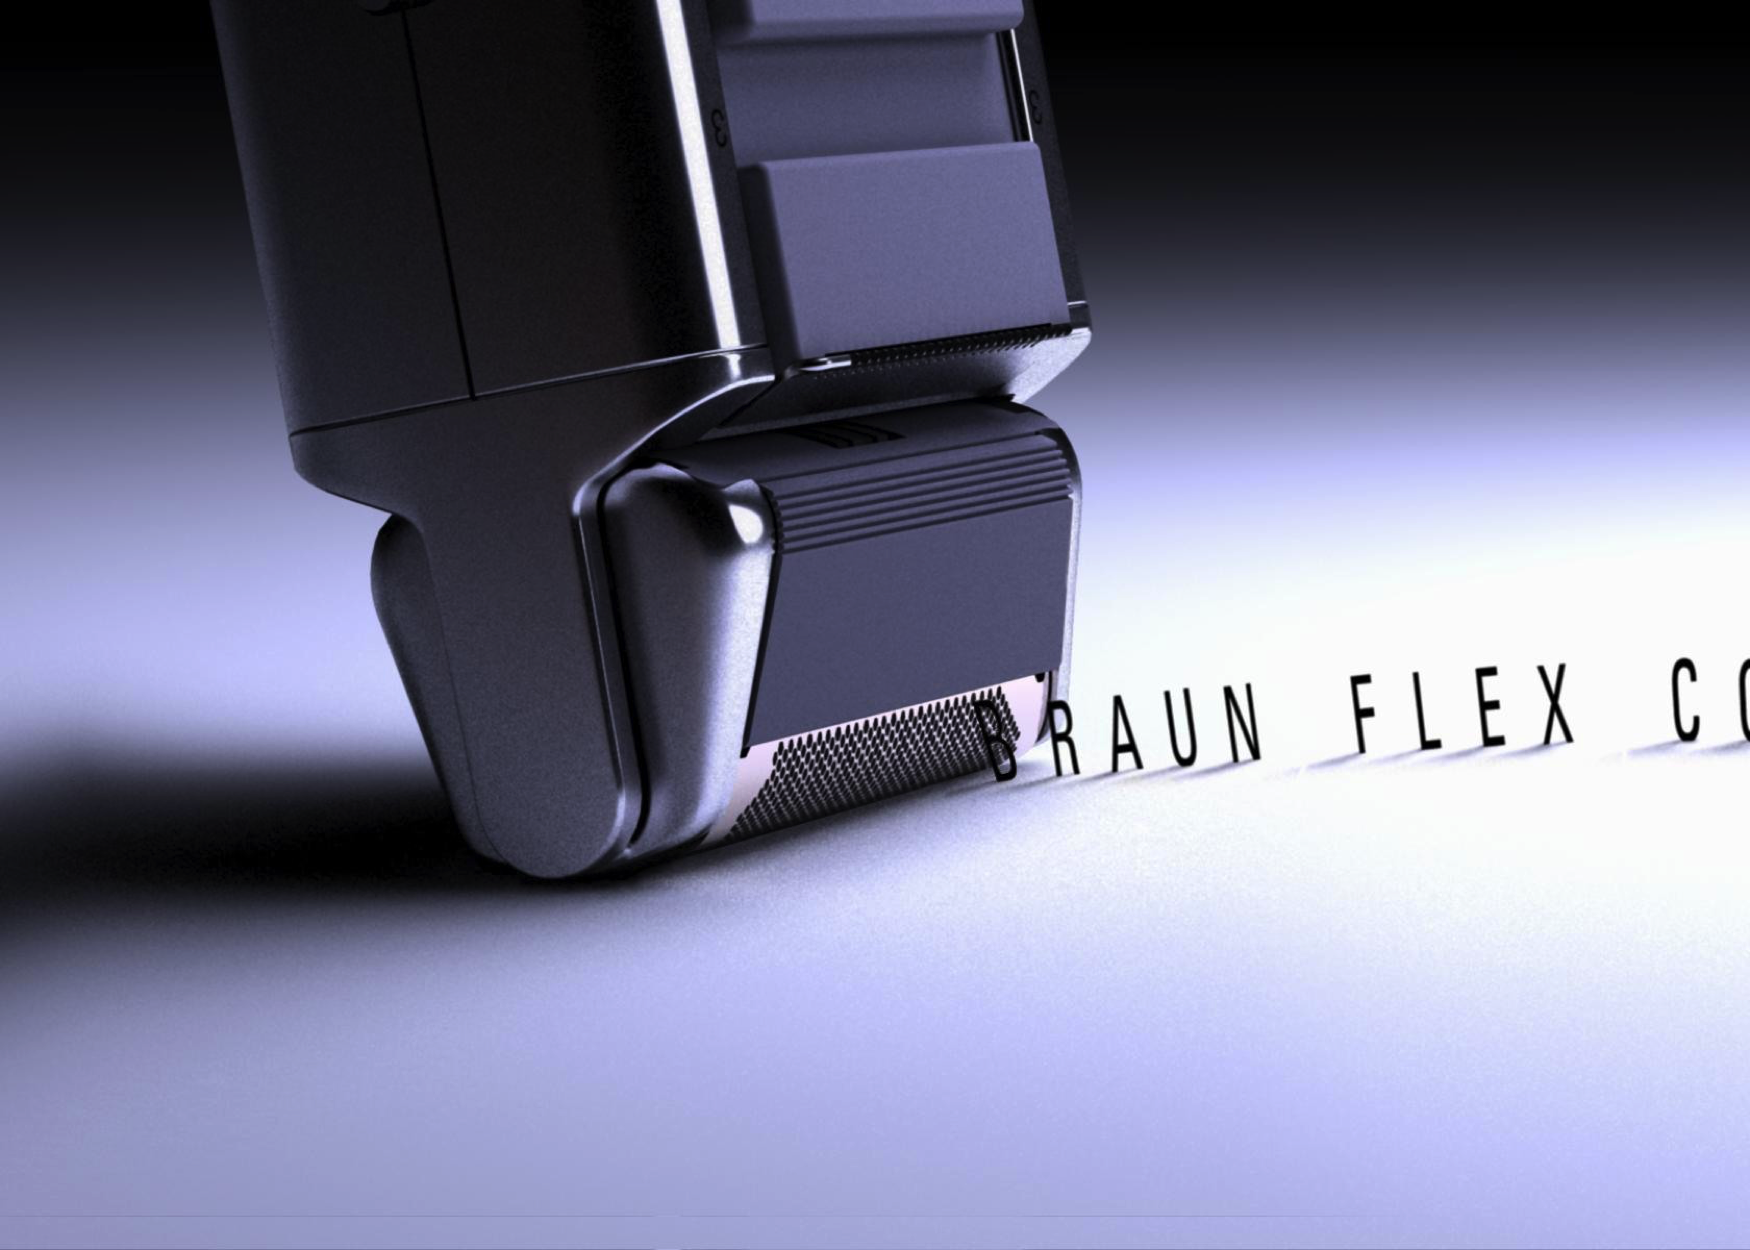
\includegraphics[width=\linewidth]{chap01/BraunRazor.png}
\end{marginfigure}
他们1998年上映的短片电影《棕兔夫人》\sidenote{译者注:Bunny。}
是在制作中使用蒙特卡洛全局照明的早期案例。
其视觉呈现与用Reyes渲染的电影和短片截然不同,获得了广泛关注。
蓝天工作室随后拍摄的故事片沿用了该方法。
不幸的是,蓝天工作室从未公开其方法的重要技术细节,限制了其扩大影响。

21世纪00年代初期,大量工作室使用主打视觉效果的\emph{mental ray}光线追踪渲染器系统。
它是实现了复杂全局光照算法的非常高效的光线追踪器。
其开发者主要关注计算机辅助设计和产品设计应用,
因此它缺乏电影制作所需的处理极其复杂场景和极多纹理贴图之类的特性。

《棕兔夫人》之后,2001年迎来了另一个分水岭,
Marcos Fajardo带着他早期版本的\emph{Arnold}渲染器来到了SIGGRAPH
\sidenote{译者注:即ACM Special Interest Group on Computer Graphics and Interactive Techniques,
    计算机图形学与交互技术特别兴趣小组,成立于1969年,其前身ACM SICGRAPH成立于1967年。}。
他展示了蒙特卡洛图像合成课程上的图片,
不仅有复杂几何体、纹理和全局光照,而且几十分钟内就能完成渲染。
尽管这些场景不如当时电影制作中用的那么复杂,
但他的结果证明了复杂场景中全局光照有许多创造性机会。

Fajardo把\emph{Arnold}带到了索尼影业图像工作室\sidenote{译者注:Sony Pictures Imageworks。},
开始将其转化为可用于制作的基于物理的渲染系统。
高效运动模糊、可编程着色、支持大量复杂场景和延迟加载场景体
以及在内存只保留一小部分场景纹理时支持纹理缓存等,这些都是需要解决的重要领域。
\emph{Arnold}在电影《怪兽屋》\sidenote{译者注:即Monster House,于2006年上映。}得到首次应用,
现在一般作为一款产品提供。

21世纪00年代中期,皮克斯\sidenote{译者注:即Pixar Animation Studios,皮克斯动画工作室,
    于1986年成立,
    % 前身为卢卡斯影业计算机部图形学小组(The Graphics Group of Lucasfilm Computer Division),
    代表作有
    《玩具总动员》(Toy Story)、
    《海底总动员》(Finding Nemo)、
    《超人总动员》(The Incredibles)、
    《赛车总动员》(Cars)、
    《机器人总动员》(WALL·E)、
    《飞屋环游记》(Up)、
    《头脑特工队》(Inside Out)、
    《心灵奇旅》(Soul)等。}的
\emph{RenderMan}渲染器开始支持混合栅格化和光线追踪算法
并包括了大量解决复杂场景下求解全局光照的创新算法。
\emph{RenderMan}最近遵循pbrt的一般系统架构\citep{10.1145/2776880.2792699}
\sidenote{译者注:此处参考文献笔者改为了同名同源发表但作者名单更全的文献。}
被重新编写为基于物理的光线追踪器。

基于物理的蒙特卡洛渲染方法成功用于制作的一大原因是
它们最终提高了艺术家们的生产力。
一些重要因素是:
\begin{itemize}
    \item 涉及的算法本质上只有一个质量旋钮:每个像素取多少次采样;
          这对艺术家们很有用。通过每个像素只采几个样本,
          光线追踪算法也适合渐进式改善和快速计算粗略预览图;
          基于栅格化的渲染器则没有等效功能。
    \item 采用基于物理的反射模型让设计表面材料变得简单。
          早前,当使用能量未必守恒的反射模型时,
          一个物体可能被放置在单光源环境下来调节其表面的反射参数。
          该物体在那个环境下可能看起来不错,
          但移到另一个光照环境时常常会显得完全不对,
          因为表面实际上反射了太少或太多的能量:
          表面属性被设为不合理的值。
    \item 光线追踪计算的阴影质量比栅格化方法好得多。
          取消微调阴影贴图分辨率、偏置以及其他参数的需求把灯光艺术家们的烦人任务消除了。
          此外,基于物理的方法本身还给他们带来了反射光和其他柔光效果,
          无需艺术手工调整过程。
\end{itemize}

在编写本书时,基于物理的渲染已广泛运用于计算机生成图像的电影制作当中;
\reffig{1.22}和\reffig{1.23}展示的图像就来自两部近年使用了基于物理方法的电影。
\begin{figure}[htbp]
    \centering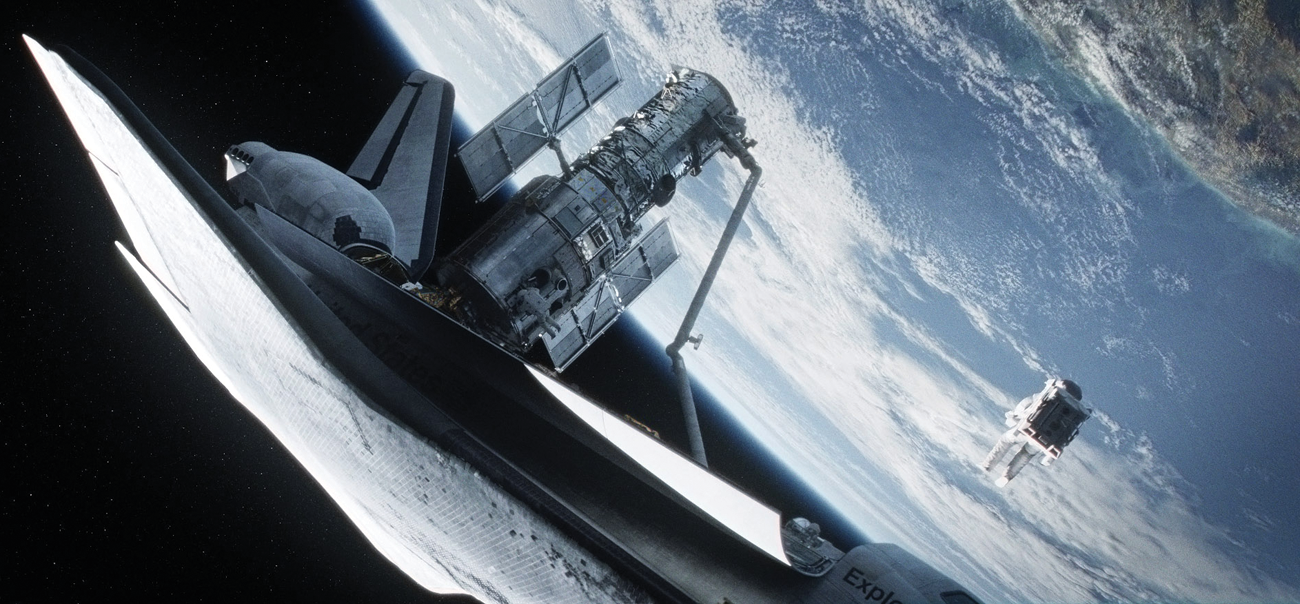
\includegraphics[width=\linewidth]{chap01/gravity.png}
    \caption{《地心引力》(Gravity, 2013)以计算机生成
        具备体积散射和大量各向异性金属表面的壮观逼真太空环境图像为特色。
        它由支持全局照明的基于物理的渲染系统\emph{Arnold}生成。
        该图由华纳兄弟(Warner Bros.)和Framestore提供。
    }
    \label{fig:1.22}
\end{figure}
\begin{figure}[htbp]
    \centering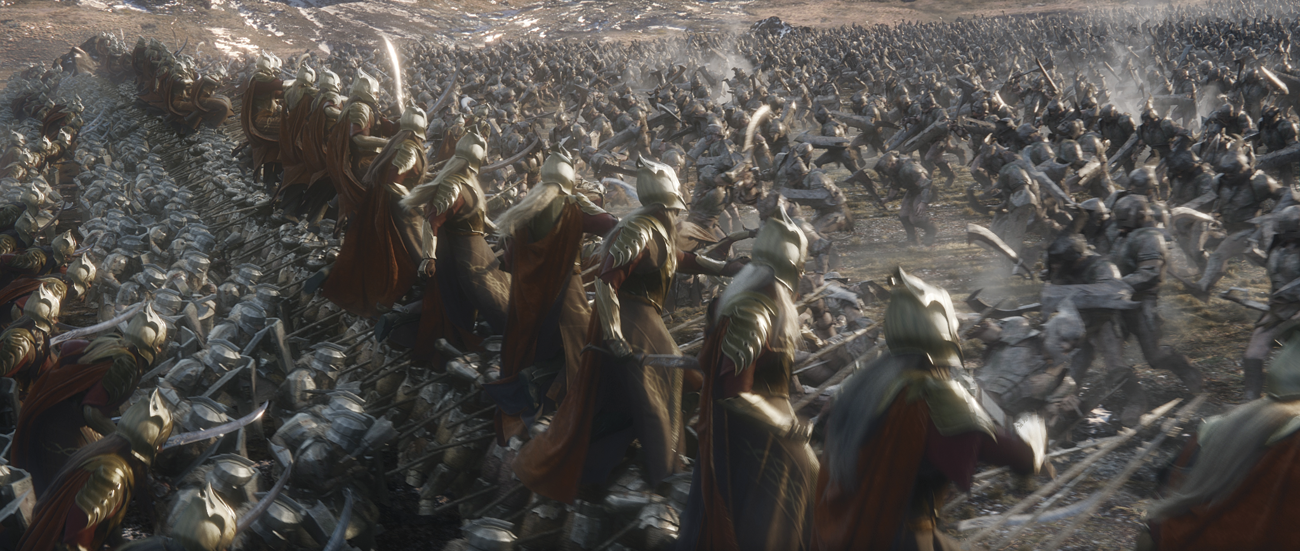
\includegraphics[width=\linewidth]{chap01/hobbit.png}
    \caption{来自《霍比特人3:五军之战》(The Hobbit: The Battle of the Five Armies, 2014)的
        该图也是用基于物理的渲染系统渲染得到的;
        这些角色以异质表面下的散射和大量几何细节为特点。
        图像由维塔数码(Weta Digital)制作,由华纳兄弟和米高梅(Metro-Goldwyn-Mayer)提供。}
    \label{fig:1.23}
\end{figure}

